% Anleitung zu den beiden TI-Nspire-Lua-Skripten
%   Tragwerksskript/Biegelinieneu.lua  und  Querschnitte/Querschnitt.lua
% Uebersetzen mit pdflatex (zweimal, wegen Inhaltsverzeichnis und Verweisen).
% Bilder: \bildplatz{dateiname}{Bildunterschrift} setzt einen Platzhalterrahmen.
%         Zum Einfuegen eines echten Bildes die Zeile durch
%         \begin{figure}[htbp]\centering\includegraphics[width=0.8\linewidth]{bilder/datei}\caption{...}\end{figure}
%         ersetzen.


%Systemansicht noch am anfang irgendwo erwähnen



\documentclass[11pt,a4paper]{article}

\usepackage[utf8]{inputenc}
\usepackage[T1]{fontenc}
\usepackage[ngerman]{babel}
\usepackage[a4paper,margin=2.4cm]{geometry}
\usepackage{amsmath}
\usepackage{amssymb}
\usepackage{array}
\usepackage{booktabs}
\usepackage{longtable}
\usepackage{graphicx}
\usepackage{subcaption}   % subfigure-Umgebung fuer mehrere Bilder in einer Abbildung
\usepackage{xcolor}
\usepackage{tikz}
\usepackage[autostyle,german=quotes]{csquotes}
\usepackage[hidelinks]{hyperref}

\setlength{\parindent}{0pt}
\setlength{\parskip}{0.6em}

\newcommand{\taste}[1]{\textsf{\textbf{#1}}}
\newcommand{\code}[1]{\texttt{#1}}
\newcommand{\bildplatz}[2]{%
  \begin{figure}[htbp]
    \centering
    \fbox{\parbox[c][3.0cm][c]{0.78\linewidth}{\centering\itshape Platz für ein Bild: \texttt{#1}}}
    \caption{#2}
  \end{figure}}

\title{Anleitung\\[0.3em]\large Tragwerksskript und Querschnittsskript für den TI-Nspire CX II CAS}
\author{}
\date{}

\begin{document}
\maketitle
\tableofcontents
\newpage

%=====================================================================
\section{Grundlegendes}

\subsection{Überblick}

Das Programm deckt große Teile der TM1- und TM2-Klausur ab, dazu Teile der Statik-Klausur. Dafür
gibt es drei Module, also drei Seiten auf dem Taschenrechner:

\begin{itemize}
  \item \textbf{Tragwerksskript}: ebene Stabtragwerke und Fachwerke, Schnittgrößen,
        Verformungen, Kraftgrößenverfahren, Prinzip der virtuellen Verschiebungen, Export der Biege- und Längslinien ins CAS. Dieses Modul ist relevant für \textbf{TM1}, \textbf{TM2} und \textbf{Statik}.

  \item \textbf{Querschnittsskript}: Querschnittswerte,
        Normalspannung, Schubspannung, Schubmittelpunkt, Torsion, Kernfläche. Vor allem relevant für \textbf{TM2}, für einfache Schwerpunktaufgaben auch für \textbf{TM1}.

  \item \textbf{Spannungskreis}: ebener Spannungszustand über Schnitte eingeben, mit Tabelle,
        Spannungsscheibe und Mohrschem Kreis, falls ihr euch auch immer in die falsche Richtung dreht. Relevant für \textbf{TM2}.
\end{itemize}

Was in welchem Modul drankommt und welcher Teil des Programms dazu passt:

\begin{longtable}{p{0.10\linewidth}p{0.44\linewidth}p{0.40\linewidth}}
  \toprule
  \textbf{Modul} & \textbf{Themen} & \textbf{Im Programm} \\
  \midrule \endhead
  \textbf{TM1} & Kräftesysteme, Schwerpunkt, Lagerreaktionen und statische Bestimmtheit,
    mehrteilige Tragwerke, Fachwerke, Schnittgrößen, Prinzip der virtuellen Verrückung (PvV),
    Reibung &
    Explosionszeichnung und LGS-Export (Abschnitt~\ref{sec:Explosionszeichnung}), Fachwerke,
    $N$-/$Q$-/$M$-Verläufe, PvV mit Polplan und Arbeitssatz; Schwerpunkt im Querschnittsskript \\
  \textbf{TM2} & Flächenträgheitsmomente, Spannung, Dehnung, Mohrscher Spannungskreis,
    Elastizitätsgesetz, Biegetheorie und DGL der Biegelinie, Normalspannung und Kernfläche,
    Schubspannung (auch dünnwandig), Torsion, Drillung und Verwölbung &
    Querschnittsskript, Spannungskreis, Biegelinie und Längslinie (Rand-LGS-Export), starre
    Stäbe, Temperatur \\
  \textbf{Statik} & fast ausschließlich statisch unbestimmte Systeme: Arbeitssatz und Prinzip der
    virtuellen Kräfte, Kraftgrößenverfahren (Reduktionssatz, Symmetrie), Weggrößenverfahren/FEM,
    Galerkin, Scheiben &
    KGV mit Einheitszuständen und $\delta$-Zahlen, Systemmatrizen des WGV, richtige Steifigkeiten
    ($EI$-Verhältnisse, dehnstarr), Temperatur \\
  \bottomrule
\end{longtable}

Nicht im Programm sind Reibung, räumliche Kräftesysteme, Galerkin und Scheiben.

Für die meisten Exporte und für symbolische Berechnungen wird meines Wissens die
\textbf{CAS}-Version des Rechners gebraucht. Da bin ich mir aber nicht ganz sicher. Der Grund:
Für exakte Brüche, Symbole und die Exporte ruft das Programm den CAS-Kern des Rechners auf.

Ganz hinten (Teil~\ref{sec:Mathe}) steht, wie die Programme intern rechnen, also nicht, wie man
einen Hebelarm ausrechnet, sondern die Stellen, an denen die Rechenmethoden des Programms von denen der Vorlesung abweichen:
starre Stäbe, das Rand-LGS, der symbolische Modus, der Polplan, $q_0$ bei geschlossenen Profilen
und so weiter.



\subsection{Grundprinzip der Bedienung}

\subsubsection{Tragwerk- und Querschnittmodul}

\begin{itemize}
  \item Gezeichnet wird mit der Maus bzw. dem Touchpad, Punkte rasten auf dem Raster ein.
  \item Ein Objekt unter dem Mauszeiger (\emph{Hover}) wird hervorgehoben. \taste{Enter} öffnet
        dessen Menü. \taste{Del} löscht im Tragwerksskript das gehoverte Element, im
        Querschnittsskript das zuletzt gezeichnete (einzelne Elemente löscht ihr dort über ihr
        Menü).
  \item Obermenü mit Taste \taste{o}. In Menüs bewegt man sich mit den Pfeiltasten \taste{$\uparrow$}/\taste{$\downarrow$};
        \taste{$\leftarrow$}/\taste{$\rightarrow$} blättert die Seiten. \taste{Enter} öffnet eine
        Eingabe oder schaltet einen Wert um, ein zweites \taste{Enter} übernimmt die Eingabe.
  \item Auf der Zeichenfläche selber wird mit \taste{$\uparrow$}/\taste{$\downarrow$} und
        \taste{$\leftarrow$}/\taste{$\rightarrow$} navigiert und mit \taste{+}/\taste{-} gezoomt.
  \item \taste{h} (Home) zoomt automatisch so, dass das ganze System bzw.\ der ganze Querschnitt
        ins Bild passt.
  \item \taste{Esc} bricht ab und schließt Boxen, \taste{ctrl}+\taste{Del} oder \taste{c} löscht alles.
  \item Alle Zahlenfelder akzeptieren Ausdrücke: \code{2/3}, \code{sqrt(2)}, \code{1e8},
        Dezimalkomma (\code{1,5}) und im Tragwerksskript auch Symbole wie \code{q} oder \code{EI}.
        Im Querschnittsskript geht \code{\^{}} nicht, dort schreibt ihr \code{1e6} statt \code{10\^{}6}.
\end{itemize}

%=====================================================================
\part{Tragwerksskript}

\section{Systemeingabe}

Die eigentliche Systemberechnung läuft über das WGV (kommt in Statik). Aus diesem Grund mag die
Art, Systeme zu zeichnen, manchmal etwas unintuitiv wirken, z.\,B.\ wird die $y$-Achse positiv
nach unten gezählt.

Die zwei grundlegenden Bausteine eines Systems sind Elemente bzw.\ Stäbe und Knoten. Knoten könnt
ihr überall platzieren (einfach mit dem Touchpad an eine Stelle klicken), Stäbe nur von einem
Knoten zu einem anderen (ersten Knoten anklicken, dann den zweiten). Alle weiteren Eigenschaften
des Systems wie Lagerung, Lasten und Gelenke gebt ihr entweder über die Knoten oder über die Stäbe
ein. (Ein Einfeldträger hat also zwei Knoten und einen Stab, ein 3-Gelenk-Tragwerk in seiner
einfachsten Form drei Knoten und zwei Stäbe.)

Für \textbf{Statik} sollte diese Eingabe Sinn machen.

Für \textbf{TM2} könnt ihr euch merken, dass ihr für jeden Bereich, für den ihr eine neue
Biegelinie ansetzen würdet, auch einen neuen Stab setzen müsst. Das liegt daran, dass das Programm
effektiv für alle Stäbe die DGL der Biegelinie löst. Die FEM bzw.\ das WGV (in diesem Fall zwei
direkt verwandte Verfahren) bieten nur einen etwas raffinierteren Lösungsweg als den, den man in
\textbf{TM2} lernt (Abschnitt~\ref{sec:mathe-wgv}).

Für \textbf{TM1} fällt mir leider kein besserer Hinweis ein, als einfach genügend Systeme
einzugeben, bis man ein Gefühl für die Eingabe bekommt.


\subsection{Knoten}\label{sec:Eingabe_Knoten}

Am Knoten hängt alles, was punktuell ist: Lager, Einzellasten, Federn und das Vollgelenk. Ihr
kommt ins Knotenmenü, indem ihr mit dem Zeiger über den Knoten geht und \taste{Enter} drückt,
anklicken müsst ihr nicht. Das Menü hat vier Seiten, zwischen denen ihr mit
\taste{$\leftarrow$}/\taste{$\rightarrow$} blättert.

\begin{longtable}{p{0.16\linewidth}p{0.36\linewidth}p{0.42\linewidth}}
  \toprule
  \textbf{Seite} & \textbf{Zeilen} & \textbf{Bedeutung} \\
  \midrule \endhead
  1 Geometrie & X-Koordinate, Y-Koordinate, Gelenkig, Lager X, Lager Y, Lager M &
    Koordinaten dürfen auch ein Ausdruck oder ein Symbol sein. \emph{Gelenkig} macht den Knoten
    zum Vollgelenk (alle Stabenden dort momentenfrei). Das geht nur, solange am Knoten kein
    Moment als Last steht, und an einem gelenkigen Knoten lässt sich umgekehrt kein Moment
    eingeben. Die drei Lager sind einzeln schaltbar:
    X und Y zusammen ergeben ein Festlager, nur eines davon ein Rollenlager, alle drei eine
    Einspannung. \\
  2 Lasten & Last $F_x$, Last $F_y$, Last $M$, Lastwinkel &
    Einzellasten am Knoten. Der Winkel dreht das Lastpaar $F_x$/$F_y$ mit. \\
  3 Federn & Feder $c_x$, $c_y$, $c_m$, Federwinkel &
    Weg- und Drehfedern; der Winkel dreht die Federachsen. Federwerte dürfen symbolisch sein,
    z.\,B.\ \code{3*EA*l}. \\
  4 Ergebnisse & Verschiebung, $R_\xi$, $R_\eta$, $R_m$, \code{ü\_x}, \code{ü\_y}, \code{ü\_ges},
    $\varphi$, In TI speichern &
    Ganz oben holt \emph{Verschiebung} die Knotenverschiebung als Formel aus dem Rand-LGS
    (Abschnitt~\ref{sec:knotenverschiebung}). Darunter stehen nach der Berechnung die
    Auflagerreaktionen in Lagerrichtung und die Knotenverschiebung als Zahl; ganz unten könnt ihr
    den Knoten einzeln ins CAS exportieren. \\
  \bottomrule
\end{longtable}

Ein \textbf{gedrehtes Lager} macht ihr über den Lagerwinkel: Die Lagerrichtungen $\xi$ (davor
$x$) und $\eta$ (davor $y$) drehen sich mit (positiv gegen den Uhrzeigersinn), und die
Auflagerkräfte werden auch in diesen Richtungen ausgegeben.

\taste{Del} auf einem Knoten löscht auch alle Stäbe, die daran hängen. Die übrigen Knoten
werden dabei neu durchnummeriert, damit verschieben sich auch die Lagerbuchstaben $A$, $B$, \dots\
der Explosionszeichnung.

Ich möchte hier einmal auf den Unterschied zwischen Voll- und Angelenk hinweisen: Vollgelenke
werden über den Knoten eingegeben, Angelenke über den Stab (siehe Abschnitt~\ref{sec:Eingabe_Stäbe}).
Der kleine schwarze Punkt des Knotens bedeutet, dass alle angreifenden Stäbe automatisch biegesteif
miteinander verbunden sind (Abb.~\ref{fig:Knotenverbindungen}).



\begin{figure}[h]
    \centering
    \begin{subfigure}[t]{0.2\textwidth}
        \centering
        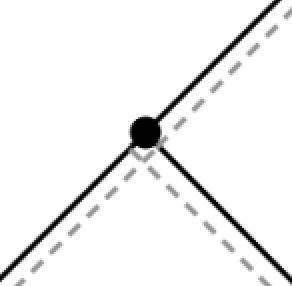
\includegraphics[height=1.2in]{./fig/Biegesteifeverbindung.png}
        \caption{Biegesteife Verbindung}
    \end{subfigure}
    \begin{subfigure}[t]{0.2\textwidth}
        \centering
        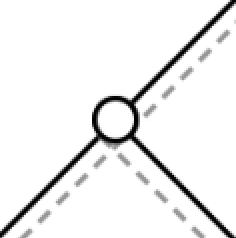
\includegraphics[height=1.2in]{./fig/Vollgelenk.png}
        \caption{Vollgelenk}
    \end{subfigure}
    \begin{subfigure}[t]{0.2\textwidth}
        \centering
        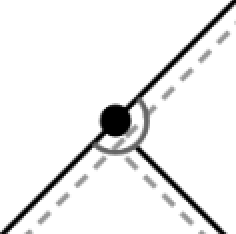
\includegraphics[height=1.2in]{./fig/Angelenk.png}
        \caption{Angelenk}
    \end{subfigure}
    \begin{subfigure}[t]{0.2\textwidth}
        \centering
        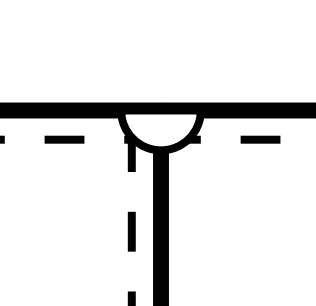
\includegraphics[height=1.2in]{./fig/Angelenk_ISD.png}
        \caption{Angelenk in ISD Klausur}
    \end{subfigure}
    \caption{Verschiedene Knotenverbindungen im Programm}
    \label{fig:Knotenverbindungen}
\end{figure}

Ich habe mein Bestes gegeben, dass die Auflager so aussehen, wie sie in den Klausuren vermutlich
auch aussehen werden. Falls das, was gezeichnet wird, gar nicht zu euren Erwartungen passt, vertraut
auf das, was ihr im Menü eingegeben habt, damit wird gerechnet.

Wenn Kräfte sowohl in $x$- als auch in $y$-Richtung eingegeben werden, zeichnet euch das Programm
den Pfeil der Resultierenden. Diesen könnt ihr (genau wie bei Auflagern positiv gegen den
Uhrzeigersinn) über den Lastwinkel drehen.

Die Auflagerkräfte $R_\xi$, $R_\eta$ und $R_m$ sollten weitestgehend selbsterklärend sein. Für
einen Lagerwinkel von $\alpha = 0^\circ$ gilt $R_\xi = R_x$ und $R_\eta = R_y$. Aufpassen:
$R_\eta$ zählt nach \emph{oben} positiv, also andersherum als die $y$-Achse des Programms, und
$R_m$ gegen den Uhrzeigersinn. Um an Auflagerkräfte dranzukommen, gibt es aber bessere Methoden
(siehe Abschnitt~\ref{sec:Explosionszeichnung}).

Die Knotenverschiebung wird in Metern angegeben, die Verdrehung in rad. Bei Stäben mit Gelenken,
gerade bei Angelenken, ist die Knotenverdrehung jedoch mit Vorsicht zu genießen
(Abschnitt~\ref{sec:mathe-gelenke}). Wollt ihr die Verschiebung als Formel, z.\,B.\
$\frac{F l^3}{3EI}$, nehmt die Zeile \emph{Verschiebung} ganz oben auf Seite~4
(Abschnitt~\ref{sec:knotenverschiebung}).




\subsection{Stäbe}
\label{sec:Eingabe_Stäbe}

Der Stab trägt alles, was über die Länge verteilt ist: Steifigkeiten, Streckenlasten, Temperatur
und die Gelenke an seinen Enden. Auch hier: Zeiger auf den Stab, \taste{Enter}, sieben Seiten.

\begin{longtable}{p{0.16\linewidth}p{0.38\linewidth}p{0.40\linewidth}}
  \toprule
  \textbf{Seite} & \textbf{Zeilen} & \textbf{Bedeutung} \\
  \midrule \endhead
  1 Steifigkeit und Lasten & $EI$, \emph{biegesteif}, $EA$, \emph{dehnsteif}, Last $q(x)$,
    Last $n(x)$, Momentenlast $m$, Bogenradius &
    $q$ wirkt quer, $n$ längs, $m$ ist ein Streckenmoment. \emph{biegesteif}/\emph{dehnsteif}
    machen den Stab starr (Abschnitt~\ref{sec:starr}); das zugehörige Feld ist dann gesperrt und
    zeigt \emph{starr}. Ein Bogenradius $\ne 0$ macht aus dem Stab einen Kreisbogen. Das geht
    nur, wenn $|R|$ mindestens die halbe Stablänge ist, sonst bleibt der Stab gerade. Das
    Vorzeichen von $R$ legt fest, zu welcher Seite der Bogen gekrümmt ist. \\
  2 Globale Linienlasten & Global $p_X$, $p_X$ projiziert, Global $p_Y$, $p_Y$ projiziert &
    Lasten in globaler Richtung, wahlweise auf die Stabachse projiziert, also genau die
    Unterscheidung \enquote{Schnee auf der Dachfläche} gegen \enquote{Schnee auf dem Grundriss}.
    Hängt die Last von $x$ ab, läuft $x$ bei projizierter Last entlang der globalen Achse ab dem
    Stabanfang ($p_Y$ waagerecht, $p_X$ senkrecht), sonst entlang des Stabes. \\
  3 Trapezlasten und Temperatur & Trapez $q$ Start/Ende, Trapez $n$ Start/Ende,
    $T_{oben}$, $T_{unten}$, $\alpha_T$, Höhe $h$ &
    Die Trapezanteile addieren sich zur konstanten Last aus Seite~1. Temperatur siehe
    Abschnitt~\ref{sec:temperatur}. \\
  4 Gelenke & M-Gelenk Start/Ende, N-Gelenk Start/Ende, Q-Gelenk Start/Ende &
    Ein M-Gelenk überträgt kein Moment, ein N-Gelenk keine Normalkraft, ein Q-Gelenk keine
    Querkraft. Das Gelenk sitzt am jeweiligen Stabende, nicht am Knoten. \\
  5 Schnittgrößen & $N_a$, $Q_a$, $M_a$, $N_b$, $Q_b$, $M_b$ & Stabendgrößen nach der Berechnung. \\
  6 Auflager-/Endkräfte & $h_a$, $v_a$, $M_a$, \dots & Dieselben Endkräfte, aber in globaler
    Richtung, praktisch fürs Freischneiden. Positiv sind am Anfang $h_a$ nach links, $v_a$ nach
    oben und $M_a$ im Uhrzeigersinn, am Ende $h_b$ nach rechts, $v_b$ nach unten und $M_b$ gegen
    den Uhrzeigersinn, also wie positive Schnittgrößen am Stab. \\
  7 Verformungen und Export & $u_a$, $v_a$, $\varphi_a$, \dots, \emph{In TI speichern} &
    Stabendverformungen; Export des einzelnen Stabes ins CAS. \\
  \bottomrule
\end{longtable}

Ein paar Dinge, die ihr zu den Seiten wissen solltet:

\begin{itemize}
  \item Die Gelenke auf Seite 4 sind die \textbf{Angelenke} aus Abb.~\ref{fig:Knotenverbindungen}:
        Sie sitzen am Stabende, der Knoten selbst bleibt biegesteif mit den anderen Stäben
        verbunden. Ein N- oder Q-Gelenk gibt es nur hier, am Knoten geht nur das Vollgelenk. Das liegt daran,
        dass sich N- und Q-Gelenke auf die Richtung des Stabes beziehen (längs bzw.\ quer zur
        Stabachse), ein Knoten hat aber keine Richtung.
  \item Für \textbf{TM1} solltet ihr nicht an den Biege- und Dehnsteifigkeiten rumspielen, weder im Stab noch im Obermenü.
        Solltet ihr dort doch einmal etwas eingegeben haben, drückt am besten im Obermenü (Seite~1) einmal auf \emph{Starr-Modus: Aktivieren}.
        An diese Zahlen ist eine Warnung gekoppelt, die kommt, wenn ihr versucht, ein statisch unbestimmtes System zu berechnen. In der \textbf{TM1} habt ihr dann etwas falsch eingegeben.
  \item Im Zahlenmodus dürfen Lasten von $x$ abhängen (z.\,B.\ \code{x\^{}2} oder \code{2*x+1}),
        $x$ läuft dabei vom Stabanfang aus. Im symbolischen Modus geht das nicht
        (Abschnitt~\ref{sec:symbolisch}).
  \item \textbf{Lasten auf Bögen} gehen in die Rechnung ein. $q$ wirkt quer zum Bogen, also
        radial, $n$ tangential. Trapezlasten laufen linear über die Bogenlänge, $p_X$ und $p_Y$
        wirken in ihrer globalen Richtung (projiziert je Grundriss- bzw.\ Höhenlänge), dazu $m$ und
        Temperatur. Eigengewicht ist $p_Y = g$ je Bogenlänge. In einer Lastfunktion ist $x$ auf dem
        Bogen der \textbf{Winkel ab Stabanfang im Winkelmodus des Rechners}, also dasselbe wie $p$
        bei \code{M\_bogen1(p)}. Eine radiale Last $2\cos\varphi$ gebt ihr als \code{2*cos(x)} ein,
        das stimmt in DEG und RAD. Ein Polynom wie \code{x/90} hängt dagegen vom Modus ab (DEG:
        $x$ von 0 bis 90). Mit Bögen nur Zahlen, ein Symbol wie \code{q} schaltet den symbolischen
        Modus ein, und der kann keine Bögen.
  \item Gerechnet wird der Bogen als Kette gerader Teilstäbe (Obermenü Seite~3, Segmente für
        Bögen, Standard 20). Konstante radiale Lasten sind damit exakt, Eigengewicht und tangentiale
        Lasten bis auf etwa 0,1\,\% (Einspannmoment eines Viertelkreises unter Eigengewicht bei 20
        Segmenten um 0,04\,\% zu groß). Braucht ihr mehr Stellen, stellt mehr Segmente ein.
\end{itemize}

\taste{f} dreht den Stab unter dem Zeiger um: Anfang und Ende tauschen, alles andere bleibt so, wie
es eingegeben ist. Die gestrichelte Faser wandert also auf die andere Seite, und Lasten, Gelenke und
Temperatur beziehen sich danach auf die neue Richtung: Eine Querlast $q$ zeigt dann zur anderen
Seite, ein Gelenk am Stabanfang sitzt jetzt am anderen Knoten. Am besten dreht ihr Stäbe deshalb,
bevor ihr Lasten und Gelenke eingebt. Danach muss neu gerechnet werden (\taste{b}).
Diese sollte immer mit der gestrichelten Faser der Aufgabe (falls gegeben) übereinstimmen
bzw. mit dem gegebenen KOS bei Biegelinienaufgaben.

Für \textbf{TM2}: Die gestrichelte Faser muss, wenn ein KOS gegeben ist, immer auf der Seite sein, in die die $z$-Achse (bzw.\ $w$) des KOS zeigt.

An dieser Stelle möchte ich darauf hinweisen, dass diese KOS manchmal etwas fragwürdig gewählt werden.
Es kann vorkommen, dass die $y$-Achse des gegebenen KOS in die Bildebene hineinzeigt (das kann man mit der Rechte-Hand-Regel prüfen).
Ist dies der Fall, müsst ihr das System spiegelverkehrt zeichnen (vgl.\ Bsp.~\ref{ex:Biegelinienaufgabe}).

Sollte in einer Aufgabe mal sowohl gestrichelte Faser als auch KOS gegeben sein und diese passen nach der oben beschriebenen Regel
nicht zusammen, will der Aufgabensteller euch entweder eine Falle stellen oder hat selber nicht richtig aufgepasst (TM2 SoSe23, Nr.~6).

\subsection{Fachwerke}\label{sec:fachwerk}

Für Fachwerke (\textbf{TM1}) gibt es im Obermenü Seite~1 den \emph{Fachwerk-Modus}. Einschalten
macht alle vorhandenen Knoten zu Vollgelenken, und jeder neue Knoten ist automatisch eins. Beim
Ausschalten bleiben die Gelenke, wie sie sind.

Nach \taste{b} steht in der Systemansicht auf jedem Stab seine Stabkraft: \textcolor{blue}{blau}
bei Zug, \textcolor{red}{rot} bei Druck und eine grüne \emph{0} bei Stäben, die sich erst nach der
Rechnung als Nullstäbe herausstellen. Nullstäbe, die man schon ohne Rechnung erkennt, streicht das
Programm mit einem grünen Kreuz durch. Dafür wendet es die bekannten Regeln an, und zwar so lange,
bis kein neuer Nullstab mehr dazukommt:

\begin{itemize}
  \item unbelasteter Knoten ohne Lager mit zwei Stäben, die nicht auf einer Geraden liegen: beide
        sind Nullstäbe,
  \item Knoten mit zwei Stäben, an dem die Last (oder die Kraft eines Rollenlagers) in Richtung
        des einen Stabes wirkt: der andere ist ein Nullstab,
  \item unbelasteter Knoten ohne Lager mit drei Stäben, von denen zwei auf einer Geraden liegen:
        der dritte ist ein Nullstab.
\end{itemize}

Knoten, an denen ein Stab mit Streckenlast oder Temperatur hängt, lässt das Programm dabei aus.
Fragt eine Klausuraufgabe nach den Nullstäben, die man ohne Rechnung erkennt, zählen also nur die
grün durchgestrichenen Stäbe. Eine grüne \emph{0} ohne Kreuz ist erst ein Ergebnis der Rechnung.

In der Explosionsansicht zeichnet das Programm die Stabkräfte als Pfeile an den Knoten, auf
Seite~1 in ihrer wirklichen Richtung, auf Seite~2 alle als Zug. Das ist genau das
Knotenschnittverfahren, und der Export \emph{LGS-Matrix} schreibt dazu die Knotengleichgewichte mit
den Stabkräften \code{S\_i} (Zug positiv) heraus (Abschnitt~\ref{sec:lgs-matrix}).

\subsection{Systeme speichern und öffnen}\label{sec:system-speichern}

Das Programm bietet die Möglichkeit, Systeme zu speichern. Im Obermenü (\taste{o})
stehen auf Seite 4 ganz unten zwei Zeilen:

\begin{itemize}
  \item \emph{System speichern als:} \taste{Enter}, eine Nummer eintippen (z.\,B.\ \code{3}),
        \taste{Enter}. Das ganze System landet als Text in der Variable \code{system3} des
        Dokuments: Knoten, Stäbe, Lager, Gelenke, Lasten, Federn, Steifigkeiten, starre Stäbe,
        Temperatur, dazu Raster, Standard-$EA$/$EI$, die Schalter \emph{Fachwerk-Modus},
        \emph{Standard-EA dehnstarr} und \emph{Starre Stäbe (Export)} und der Bildausschnitt.
  \item \emph{System öffnen:} Nummer eintippen, und das aktuelle System wird durch \code{system3}
        ersetzt. Danach wird wie nach jeder Änderung neu gerechnet.
\end{itemize}

Die Variable gehört zum Dokument: Sie bleibt erhalten, wenn ihr das Skript schließt, und wird mit
dem \code{.tns} gespeichert (das Dokument also auch wirklich speichern). Rechenergebnisse und
KGV-Zustände werden nicht mitgespeichert, sie entstehen beim Öffnen neu. In der Variable steht ein
Text wie \code{TWS1;G:rasterMass=\#1,\dots;K:x=\#2,lager\_y=T;\dots}, darin steht nur, was vom
Standard abweicht. Von Hand ändern solltet ihr ihn nicht.

Praktisch für die Klausurvorbereitung: Aufgaben einmal eingeben und unter \code{system1},
\code{system2}, \dots\ ablegen. Das ist vor allem für die klassischen \textbf{TM2}-Temperatur- und Spannungsaufgaben hilfreich (vgl.\ Bsp.~\ref{ex:Temperaturaufgabe}).
Aufpassen: \code{system1} ist eine ganz normale Variable. Speichern
unter einer schon benutzten Nummer überschreibt ohne Nachfrage, und ein \code{DelVar system1} im
Calculator löscht das System.

\section{Berechnung, Ansichten und Diagramme}

\taste{b} rechnet. Das kann gerade bei symbolischen Berechnungen schon mal ein paar Sekunden dauern.
Falls sich der Taschenrechner aufhängt, drückt den Reset-Knopf auf der Rückseite. Gespeicherte Dokumente gehen dabei nicht
verloren, ungespeicherte Änderungen am offenen Dokument können aber verloren gehen.

Oben links steht, welche Ansicht gerade aktiv ist (z.\,B.\ \emph{Modus: System} oder
\emph{Modus: M}). Ist diese Schrift \textcolor{red}{rot}, hat sich das System seit der letzten
Berechnung geändert, und die angezeigten Verläufe und Werte gehören noch zum alten Stand. Dann
einfach nochmal \taste{b} drücken.

Oben rechts steht der Grad der statischen Unbestimmtheit $n$. Das Programm zählt ihn über Stäbe und
Knoten ab:
\[
  n = r + 3s - 3k - g
\]
mit $r$ Lagerreaktionen (Federn zählen mit), $s$ Stäben, $k$ Knoten und $g$ gelösten Bindungen:
jedes Stabendgelenk (M, N oder Q) zählt eine, ein Vollgelenk mit $m$ Stäben $m-1$. Geht ihr mit dem
Zeiger darüber, zeigt das Programm nach der Berechnung dieselbe Zahl in der Form aus \textbf{TM1},
$n = r + z - 3p$ mit $p$ Scheiben (dort zählen bei $r$ nur die Lager). Im Fachwerkmodus steht dort
stattdessen die Fachwerkformel $n = s + r - 2k$.

Die Zahl in Klammern dahinter kommt vom Auto-KGV-Löser (Abschnitt~\ref{sec:kgv}): Er sucht bei
jedem \taste{b} ein statisch bestimmtes Hauptsystem und zählt, wie viele Bindungen er dafür wirklich
lösen musste. Das Abzählkriterium ist nur notwendig, nicht hinreichend. Weichen die beiden Zahlen
voneinander ab, lohnt sich also ein zweiter Blick auf das System. Die Klammer schaltet ihr im
Obermenü mit \emph{Anzeige N} ein und aus. Bei sehr großen Systemen kostet die Suche nach dem
Hauptsystem viel Zeit, weil das Programm dafür das System immer wieder neu zerlegt. Braucht ihr die
Zahl nicht, schaltet \emph{Anzeige N} dann einfach aus.

Danach stehen euch diese Ansichten zur Verfügung:

\begin{longtable}{p{0.12\linewidth}p{0.84\linewidth}}
  \toprule
  \textbf{Taste} & \textbf{Ansicht} \\
  \midrule \endhead
  \taste{s} & Systemansicht \\
  \taste{n} & Normalkraft $N$ \\
  \taste{q} & Querkraft $Q$ \\
  \taste{m} & Moment $M$ \\
  \taste{w} & Biegelinie $w$ \\
  \taste{u} & Längsverformung $u$ \\
  \taste{e} & Explosionsansicht: alle Stäbe freigeschnitten, mit \taste{e} blättert ihr die
              Seiten durch \\
  \taste{t} & Beschriftungen in der Explosionsansicht ein- und ausblenden \\
  \taste{v} & Kinematik bzw.\ Verschiebungszustand (PvV) \\
  \taste{p} & Polplan \\
  \taste{l} & Gleichgewichtsbedingungen der Teilsysteme anzeigen, dieselben wie im Export
              \emph{LGS-Matrix} (Pfeiltasten scrollen) \\
  \bottomrule
\end{longtable}

Für \textbf{TM1} sind die Verläufe $N$, $Q$ und $M$, die Explosionszeichnung
(Abschnitt~\ref{sec:Explosionszeichnung}) und für das PvV der Polplan und der Verschiebungszustand
(Abschnitt~\ref{sec:pvv})
die Hauptsache.\\
Für \textbf{TM2} kommen Biegelinie $w$ und Längsverformung $u$ dazu.

Im Obermenü (\taste{o}) stellt ihr das Programm ein. Es hat vier Seiten:

\begin{longtable}{>{\raggedright\arraybackslash}p{0.16\linewidth}>{\raggedright\arraybackslash}p{0.78\linewidth}}
  \toprule
  \textbf{Seite} & \textbf{Zeilen} \\
  \midrule \endhead
  1 Einstellungen & \emph{Raster} (Rasterabstand in m); \emph{Alle EA setzen}, \emph{Alle EI
    setzen} (gilt für alle vorhandenen und alle neuen Stäbe, auch symbolisch); \emph{Starr-Modus:
    Aktivieren} (setzt $EA$ und $EI$ aller Stäbe auf $10^8$, Abschnitt~\ref{sec:starr});
    \emph{Auto-KGV} (Abschnitt~\ref{sec:kgv}); \emph{Anzeige N} (Grad der Unbestimmtheit aus dem
    Auto-KGV-Löser in Klammern oben rechts, siehe oben; kostet bei großen Systemen Rechenzeit); \emph{Schnittgrößen-Modus} (\emph{Hover}
    zeigt den Wert unter dem Zeiger, \emph{Start\&End} die Stabendwerte);
    \emph{Fachwerk-Modus} (Abschnitt~\ref{sec:fachwerk}) \\
  2 Exporte & alle Exporte ins CAS (Abschnitt~\ref{sec:export}) \\
  3 Darstellung & Toleranz beim Erraten von Brüchen ($10^{-x}$, nur für den letzten Versuch,
    siehe unten); Punkte pro Stab für die
    Verläufe; Zoomschritt normal und in der Explosionsansicht; Bemaßung an/aus; Segmente für
    Bögen; Zahlenformat (Wurzelbrüche, nur Brüche, Dezimal); Maximalwerte an/aus; Rasterpunkte
    (keine, normal, dick: auf manchen Displays sieht man die normalen Punkte kaum) \\
  4 Weiteres & Polstrahlen zeichnen (keine, notwendige, alle); Skalierung der Verläufe;
    \emph{Standard-EA dehnstarr} und \emph{Starre Stäbe (Export)} (Abschnitt~\ref{sec:starr});
    System speichern und öffnen (Abschnitt~\ref{sec:system-speichern}); \emph{Variablen löschen}:
    löscht nach einem zweiten \taste{Enter} alle Variablen, die das Skript angelegt hat (Exporte
    wie \code{wneu1}, \code{randbed}, \code{lgs}, \code{ux\_k1}, Matrizen, Hilfsvariablen).
    Gespeicherte Systeme \code{system<Nr>} und eure eigenen Variablen bleiben \\
  \bottomrule
\end{longtable}

Zum Zahlenformat: Das Programm rechnet, wenn ihr als Lasten normale Zahlen eingebt, nicht alles in exakten Brüchen aus.
Das Programm nimmt hinterher das Ergebnis als Kommazahl und versucht, einen schönen Bruch zu \enquote{erraten}. Diesen muss es nicht immer geben.
Vielleicht findet das Programm aufgrund von numerischen Abweichungen den eigentlichen Bruch auch gar nicht.
Dabei versucht es der Reihe nach einen exakten Bruch, bei \emph{Wurzelbrüche} dann die Wurzel eines
Bruchs und erst zum Schluss einen Bruch mit kleinem Nenner (höchstens 100), der nur bis auf die
eingestellte \emph{CAS Bruch-Toleranz} $10^{-x}$ stimmen muss. Nur bei diesem letzten Versuch wirkt
die Toleranz, und trotz des Namens rechnet dabei nicht das CAS. Im Format \emph{Dezimal} spielt sie
keine Rolle.
Verwendet die Option für Wurzelbrüche und Brüche also nur, wenn ihr euch zutraut, selber zu erkennen, ob der ausgegebene Bruch stimmen könnte.
Wenn die Zahlen riesig werden, fängt es wegen dieser Funktion manchmal an, etwas zu hängen.
Dann solltet ihr ausprobieren, die Einstellung einfach auf Dezimal zu stellen. Genaueres dazu in Abschnitt~\ref{sec:mathe-symbolisch}.


\subsection{Schnittkräfte}
Schnittgrößen, also die Verläufe von $N$, $Q$ und $M$, sind für \textbf{TM1} wohl das Wichtigste.
Mit den entsprechenden Tasten zeichnet euch das Programm diese direkt. Dabei ist es wichtig, darauf zu achten,
dass die Orientierung der gestrichelten Faser zu der der Aufgabe passt, sonst macht ihr Vorzeichenfehler.
Standardmäßig ist für die Darstellung \emph{Start\&End} eingestellt. So solltet ihr das in der Klausur auch zeichnen.
Bei zwei benachbarten Stäben überlappt sich die Beschriftung der Endwerte manchmal etwas.
Wenn ihr mit der Maus über einen Stab geht, werden im \emph{Start\&End}-Modus nur der Verlauf und die Randwerte dieses Stabes angezeigt.

Im Modus \emph{Hover} könnt ihr euch Werte merken: Ein Klick auf einen Stab in der $N$-, $Q$- oder
$M$-Ansicht setzt dort eine Marke, an der der Wert stehen bleibt (beim Bogen mit der Bogenlänge
$s$). So vergleicht ihr mehrere Stellen, ohne mit der Maus hin und her zu fahren. Die Marken
verschwinden erst, wenn ihr den Stab oder alles löscht.

Die Maximalwerte der Biegelinie $w$ und der Längsverformung $u$ stehen in Millimetern.
Fast waagerechte Linien sehen auf dem Rechner etwas treppig aus: Der Bildschirm zeichnet Linien
ohne Kantenglättung, eine flache Gerade springt deshalb immer wieder um ein Pixel. Mehr Punkte
pro Stab ändern daran nichts. Eine größere \emph{Verlauf-Skalierung} (Obermenü Seite~4) macht
die Linie steiler, dann werden die Stufen kürzer und gleichmäßiger.


\subsection{Explosionszeichnung}\label{sec:Explosionszeichnung}

Die Explosionszeichnung (\taste{e}) ist vor allem für \textbf{TM1} hilfreich.
Sie ist der schnellste Weg, an Auflager- und Gelenkkräfte zu kommen.
Das Programm schneidet jeden Stab bzw.\ jedes Teilsystem frei und zeichnet alle Kräfte ein, die daran
angreifen. Also genau das Bild, das ihr sonst von Hand malt. Mit \taste{e} blättert ihr, mit
\taste{t} blendet ihr die Beschriftungen ein und aus.

\begin{itemize}
  \item \textbf{Seite~1} zeigt die Ergebnisse: Jeder Pfeil zeigt in die Richtung, in die die Kraft
        \emph{wirklich} wirkt, beschriftet mit dem Betrag (im symbolischen Modus mit dem
        symbolischen Wert).
  \item \textbf{Seite~2} zeigt denselben Freischnitt als Ansatz: Jede Kraft hat ihren Namen
        ($A_h$, $A_v$, $M_A$, $Gx_1$, $Gn_2$ \dots) und zeigt in ihre \emph{positive} Richtung.
        Also so, wie ihr die Unbekannten von Hand antragt, bevor ihr wisst, welches Vorzeichen
        herauskommt.
\end{itemize}

Für die Klausur heißt das: Falls ihr selber rechnen wollt, stellt euer Gleichgewicht auf, vergleicht eure Skizze mit Seite 2
(gleiche Namen, gleiche Richtungen) und eure Ergebnisse mit Seite 1.\\
Das Aufstellen der GGW-Bedingungen kann euch das Programm aber auch abnehmen. Der Export \emph{LGS-Matrix}
(Abschnitt~\ref{sec:lgs-matrix}) schreibt die Gleichungen mit passenden Namen ins CAS. Wie
das Programm die Teilsysteme bildet, steht in Abschnitt~\ref{sec:mathe-gleichgewicht}.

Die positiven Richtungen auf Seite 2 sind immer dieselben:

\begin{itemize}
  \item \textbf{Lager} heißen nach ihrer Reihenfolge $A$, $B$, $C$, \dots: $A_h$ in Lagerrichtung
        (ungedreht nach rechts), $A_v$ nach oben, $M_A$ gegen den Uhrzeigersinn.
  \item \textbf{Gelenkkräfte} ($Gx$, $Gy$ bzw.\ $Gn$, $Gq$, $Gm$) wirken am ersten Stab mit Gelenk
        am Knoten wie positive Schnittgrößen, am Stabanfang nach links bzw.\ oben, gegen die
        Stabachse und im Uhrzeigersinn, am Stabende umgekehrt. Und auf der anderen Seite des
        Gelenks genau entgegengesetzt (actio = reactio). Treffen mehr als zwei Teile in einem
        Gelenk zusammen, hat jeder Stab seine eigenen Gelenkkräfte (Anhang \code{s1}, \code{s2},
        \dots\ für das Teilsystem).
  \item \textbf{Lasten und Lager an einem Gelenkknoten} hängen am ersten Stab mit Gelenk dort.
\end{itemize}

Manchmal werden in Klausuraufgaben Lager und Gelenke bereits in der Aufgabenstellung benannt.
Dann ist es sinnvoll, entweder das System in der jeweiligen Reihenfolge einzugeben oder die Namen im Nachhinein anzupassen.

\textbf{Streckenlasten stehen dort als Resultierende:} Statt der Lastfläche seht ihr einen Pfeil
auf der Wirkungslinie, beschriftet mit $R = \dots$, und die Lage hängt in der Maßkette unter dem
System. Den Hebelarm könnt ihr also direkt ablesen. Das gilt für die Querlast $q$, die Längslast
$n$ und die globalen Linienlasten $p_X$, $p_Y$; ein Streckenmoment $m$ wird zu einem Moment
$M = m\,l$ in Stabmitte. Bei einer Dreieckslast sitzt der Pfeil, wo er hingehört, nämlich bei
$x_R = S/R$ vom Stabanfang aus, und bei einer Lastfunktion wie \code{x\^{}2} rechnet das
Programm $R$ und die Lage aus der Lastfunktion selbst.


Ähnlich wie bei den Diagrammen zu Schnittgrößen wird, wenn man mit der Maus über ein Teilsystem \emph{hovert},
nur dieses Teilsystem eingeblendet. Zudem wird dann auch der Punkt angezeigt, um den das Programm die Momentensumme für das jeweilige Teilsystem bildet.
Mit der Standard-Zoomeinstellung ist die Ansicht oft überfüllt. Um das Navigieren etwas zu erleichtern, ist der Zoom in dieser Ansicht aggressiver eingestellt.
Das lässt sich im Obermenü (Seite~3) aber auch manuell einstellen.

\subsection{Prinzip der virtuellen Verrückung (PvV)}\label{sec:pvv}

Das PvV kommt nur in \textbf{TM1} dran,
für \textbf{TM2} und \textbf{Statik} ist dieser Abschnitt irrelevant.

\taste{v} öffnet den Verschiebungszustand. Solange das System nicht kinematisch ist, kommt die
Meldung \emph{System ist starr! [Enter] für PvV-Modus}. Nach \taste{Enter} wählt ihr mit
einem Klick auf einem Knoten oder Stab, welche Bindung ihr lösen wollt:

\begin{itemize}
  \item am Knoten: Lager X, Lager Y, Lager M entfernen oder ein Gelenk einfügen (letzteres nur
        bei genau zwei Stäben),
  \item am Stab: M-, N- oder Q-Gelenk an Anfang oder Ende.
\end{itemize}

Danach zeigt euch das Programm die kinematische Kette und auf Wunsch den Polplan (\taste{p}).
Zeichnung, Menüs und der Export \emph{Arbeitssatz} (Obermenü Seite~2, Abschnitt~\ref{sec:arbeitssatz})
benutzen dieselben Namen und dieselben Werte:

\begin{itemize}
  \item An jedem Weg steht \emph{Name = Wert} genau wie in Spalte~3 von \code{pvv\_kin}, z.\,B.
        \code{$\delta$\_k2x = -2*l*$\varphi$\_0} an einer Knotenlast (Pfeil in Lastrichtung, bei
        gedrehtem Lastsystem mitgedreht), \code{$\delta$\_s2q} an einer Streckenlast,
        \code{$\delta$\_H}, \code{$\delta$\_V} am gelösten Lager, \code{$\delta$\_G} bzw.
        \code{$\varphi$\_G} am gelösten Gelenk.
  \item Die Drehbögen der Scheiben heißen \code{$\varphi$\_1 = -2*$\varphi$\_0} usw., die
        Bezugsscheibe \code{$\varphi$\_3 = $\varphi$\_0}; eine Scheibe, die sich nur verschiebt,
        \code{$\delta$\_2 = \dots}.
  \item Das Menü eines Knotens oder Stabes (Klick darauf) listet seine Wege, die Drehwinkel der
        beteiligten Scheiben und seine Arbeitsanteile, also die Terme, die er zu \code{w\_eq1}
        beiträgt. Das gelöste Einspannmoment heißt auch im Bild \code{M\_A}.
\end{itemize}

Alles, was ihr im Bild ablest, könnt ihr also direkt in \code{w\_eq1} einsetzen. Nicht glatte
Zahlen zeigt die Zeichnung auf vier Stellen gerundet. Das ist die schnellste Kontrolle, ob eure
Handrechnung stimmt.

Im Polplan heißen die Hauptpole \emph{HP1}, \emph{HP2}, \dots\ (Pol einer Scheibe gegenüber dem
Boden), die Nebenpole \emph{(i,j)} und die Polstrahlen \emph{g(\dots)}, beschriftet mit den Polen,
die auf ihnen liegen müssen. An den Stäben steht ihre Scheibe \emph{S1}, \emph{S2}, \dots;
\emph{S i (FEST)} heißt, die Scheibe ist unverschieblich. Welche Polstrahlen gezeichnet werden
(keine, nur die notwendigen oder alle), stellt ihr im Obermenü auf Seite~4 ein.

Wie Polplan, Verschiebungszustand und Arbeitssatz entstehen, steht in
Abschnitt~\ref{sec:mathe-polplan}.

\subsection{Kraftgrößenverfahren (KGV)}\label{sec:kgv}

Das KGV ist eines der Kernthemen von \textbf{Statik}, für \textbf{TM1} und \textbf{TM2} ist dieser
Abschnitt irrelevant. Die $\delta$-Zahlen sind genau die Arbeitsintegrale aus dem Prinzip der
virtuellen Kräfte, $\delta_{ik} = \int \frac{M_i M_k}{EI}\,dx + \int \frac{N_i N_k}{EA}\,dx +
\dots$. Das Programm bekommt sie nur auf einem anderen Weg (Abschnitt~\ref{sec:mathe-kgv}). Mit \emph{Auto-KGV} (Obermenü Seite~1) sucht sich das Programm,
nach drücken von \taste{b}, selbst ein statisch bestimmtes Hauptsystem und zeigt oben rechts den Grad der statischen Unbestimmtheit $n$. Mit den
Zifferntasten \taste{0}\,\dots\,\taste{9} (falls das System 10-fach statisch unbestimmt ist
kann man mit schnellem hintereinader drücken von z.B. \taste{1} und \taste{0} auch in diesen zustand wechseln) schaltet ihr zwischen dem Lastzustand (Zustand~0) und
den Einheitszuständen $X_i = 1$ um und könnt euch dabei jedes Mal die kompletten Schnittgrößen anzeigen lassen.

Gelöst wird in dieser Reihenfolge: Einspannmomente, Lagerkräfte, Momentengelenke und zuletzt
unbelastete Pendelstäbe. Der Export \emph{KGV-Daten} liefert $\delta_{ij}$ (\code{kgv\_delta}) und
$\delta_{i0}$ (\code{kgv\_delta0}); daraus folgt auf dem Rechner
$\underline{X} = -\delta^{-1}\,\delta_0$.

\textbf{Wichtig bei gelösten Pendelstäben:} Der Stab ist im Hauptsystem entfernt, die
Einheitskräfte greifen an seinen Knoten an. Seine eigene Längenänderung $NL/(EA)$ steckt deshalb
nicht in den Knotenverschiebungen und wird zu $\delta_{ii}$ addiert, aber nur zu diesem einen
Eintrag. Der Grund: Im Einheitszustand $i$ trägt allein der gelöste Stab~$i$ die Kraft $N = 1$,
alle anderen gelösten Stäbe sind ebenfalls aufgetrennt und damit kraftfrei. Dehnsteife Stäbe
liefern keinen Beitrag, und bei gelösten Lagern oder eingefügten Gelenken entfällt der Zusatz,
weil der Stab dort im System bleibt.

Mein Tipp für die Klausur: Das Hauptsystem, das ihr von Hand wählt, ist oft ein anderes als das
des Programms. Die Endergebnisse (Schnittgrößen, Lagerkräfte) stimmen trotzdem überein; die
einzelnen $\delta_{ij}$ könnt ihr nur vergleichen, wenn ihr dieselben Bindungen gelöst habt. Wie
das Programm das Hauptsystem wählt und die $\delta$-Zahlen berechnet, steht in
Abschnitt~\ref{sec:mathe-kgv}.

\section{Steifigkeiten, Temperatur und Symbole}

In diesem Kapitel geht es um Eingaben, die über das Zeichnen hinausgehen: wie steif die Stäbe
sind, Temperaturlasten und das Rechnen mit Symbolen.

\subsection{Steifigkeiten und starre Stäbe}\label{sec:starr}

Jeder Stab hat ein $EA$ und ein $EI$. Ab Werk sind das $EA = 10^{10}$ und $EI = 10^{8}$, das sind erst mal beliebige Werte.
Wie oben bereits erwähnt, solltet ihr in der \textbf{TM1} nicht an diesen Werten rumspielen. Für statisch bestimmte Systeme sind die Schnittgrößen
unabhängig davon, wie weich oder starr die Stäbe sind, man bekommt also, egal was eingegeben wird, die richtigen Schnittgrößen. Jedoch erscheint die Warnung \emph{Starrmodus \&
statisch unbestimmt} nur, wenn bei allen Stäben $EA$ und $EI$ mindestens $10^7$ sind (also z.\,B.\ mit den Werten ab Werk).\\
Im Obermenü Seite~1 setzt ihr beide Werte für alle Stäbe auf einmal (\emph{Alle EA setzen}, \emph{Alle EI setzen}); der Wert gilt dann auch für Stäbe, die
ihr danach noch zeichnet, und er darf symbolisch sein (\code{EA}, \code{EI}).

Der restliche Teil dieses Abschnitts ist für \textbf{TM1} irrelevant.

Für \textbf{TM2} und \textbf{Statik} wird es interessant, wenn Stäbe wirklich starr sein sollen.
Dafür gibt es im Stabmenü Seite~1 zwei Schalter:

\begin{itemize}
  \item \emph{biegesteif}: $EI \to \infty$, der Stab verbiegt sich nicht.
  \item \emph{dehnsteif}: $EA \to \infty$, der Stab ändert seine Länge nicht.
\end{itemize}

Das wirkt überall: in den Diagrammen, in den Auflagerkräften und im Export. Intern werden die
Stabenden dabei exakt gekoppelt und die Schnittgrößen aus dem Gleichgewicht bestimmt. Eine sehr
große Ersatzsteifigkeit wird bewusst \emph{nicht} verwendet, weil das neben weichen Federn zu schlecht konditionierten Matrizen
und Zahlenmüll führt. Wie genau das Programm das macht, steht in Abschnitt~\ref{sec:mathe-starr}.

Für \textbf{TM2} ist gerade bei Biegelinienaufgaben typisch, dass $EA \to \infty$ für alle Stäbe gelten soll.
Genau dafür sind die Schalter da; für alle Stäbe auf einmal gibt es \emph{Standard-EA dehnstarr} (siehe unten). In \textbf{Statik} steht beim KGV oft, dass
Normalkraftverformungen vernachlässigt werden, das ist genau \emph{Standard-EA dehnstarr}
(Obermenü Seite 4), dann stecken in den $\delta$-Zahlen nur die Biegeanteile.

Halten sich starre Stäbe \emph{gegenseitig} statisch unbestimmt (zwei dehnstarre Stäbe
hintereinander zwischen zwei Festlagern zum Beispiel), sagt das Gleichgewicht nicht, wie sie sich
die Kraft teilen. Das Programm rechnet dann so, als wären alle starren Stäbe gleich steif, genau
wie im Rand-LGS-Export, und sagt euch das in einer gelben Box.

Zusätzlich gibt es im Obermenü Seite 4 den Schalter \emph{Standard-EA dehnstarr} (ab Werk aus).
Damit gelten alle Stäbe als dehnsteif, bei denen ihr im Stabmenü kein eigenes $EA$ eingetragen
habt. Das ist praktisch, wenn in der Aufgabe steht \enquote{alle Stäbe dehnstarr, nur Stab 3 mit
$EA$}: Schalter an, und Stab 3 bekommt sein $EA$ im Stabmenü. Ein symbolisches $EA$ bleibt immer
dehnbar.

Der Schalter \emph{Starre Stäbe (Export)} (ebenfalls Seite~4) wählt das Verfahren für den
Rand-LGS-Export: \emph{direkt} (Standard, schneller) oder \emph{Grenzwert}. Beide liefern
dieselben Verschiebungen \code{wv} und \code{uv}; was bei starren Stäben in \code{wneu} und
\code{uneu} steht, unterscheidet sich aber (Abschnitt~\ref{sec:randlgs}). Halten sich starre Teile
gegenseitig statisch unbestimmt, wechselt das Programm von selbst auf den Grenzwert.

\textbf{Pendelstäbe} müsst ihr als solche kennzeichnen, nämlich mit Gelenken an beiden Enden
(M-Gelenke im Stabmenü Seite 4 oder gelenkige Knoten). Ohne Gelenke ist ein Stab immer ein
Biegestab und macht mit seinem $EI$ beim Tragverhalten mit. In \textbf{TM2} sind Klausuraufgaben manchmal so gestellt,
dass man bei einer Handrechnung ganz intuitiv so rechnet, als wäre ein Stab ein Pendelstab, selbst wenn keine Gelenke eingezeichnet sind.
Das Programm macht das natürlich nicht so. Aus diesem Grund müsst ihr überlegen, ob man an manchen Stellen ein Gelenk einfügen sollte, selbst wenn die
Aufgabenstellung das nicht direkt fordert. Für diesen Fall existieren aber auch passende Warnungen und Hinweise (siehe Bsp.~\ref{ex:Pendelstabannahme}).

\subsection{Temperatur}\label{sec:temperatur}

Im Stabmenü Seite~3 stehen $T_{oben}$, $T_{unten}$, der Ausdehnungskoeffizient $\alpha_T$ und die Querschnittshöhe $h$.
Es lassen sich also nur über den Stab konstante Temperaturen eingeben.
Es ergeben sich zwei Anteile:

\begin{align*}
  \varepsilon_T &= \alpha_T \,\frac{T_{oben} + T_{unten}}{2} && \text{(gleichmäßige Erwärmung, Längenänderung)}\\
  \kappa_T &= \alpha_T \,\frac{T_{unten} - T_{oben}}{h} && \text{(Temperaturunterschied, Krümmung)}
\end{align*}

Die Temperaturdehnung selbst erzeugt keine Kraft. Kräfte entstehen nur aus dem Teil der Verformung,
der darüber hinausgeht:
\[
  N = EA\,\bigl(u' - \varepsilon_T\bigr), \qquad M = -EI\,\bigl(w'' + \kappa_T\bigr) .
\]
Das ist wichtig, wenn ihr Schnittgrößen aus \code{uneu} bzw.\ \code{wneu} ableitet
(Abschnitt~\ref{sec:randlgs}).

\textbf{Aufpassen bei $h = 0$:} Dann gibt es keinen Gradienten, es wirkt nur die mittlere
Erwärmung. Wenn ihr einen Stab gleichmäßig um $\Delta T$ erwärmen wollt, tragt
$T_{oben} = T_{unten} = \Delta T$ ein. Schreibt ihr nur $T_{oben} = \Delta T$ und lasst $h = 0$,
wirkt nur $\Delta T/2$. Darauf weist euch eine gelbe Box hin.

Temperatur darf auch symbolisch sein (\code{dt}, \code{t1}, \code{a}). Die für die Temperatur passende Variable \code{T}
ist aber intern bereits belegt und kann aus diesem Grund nicht eingegeben werden.
Mit einem symbolischen $\Delta T$ könnt ihr genau die Klausurfrage beantworten, bei der ein $\Delta T$ gesucht ist: erst symbolisch rechnen, dann im
CAS nach \code{dt} auflösen (Abschnitt~\ref{sec:export}, Bsp.~\ref{ex:Pendelstabannahme}).

\subsection{Symbolischer Modus}\label{sec:symbolisch}

Sobald in irgendeinem Feld ein Symbol steht (\code{q}, \code{F}, \code{EI}, \code{dt} \dots),
schaltet das Programm um. Oben rechts steht dann \emph{symb.} Für den Benutzer macht das eigentlich keinen großen Unterschied.
Es gibt aber ein paar Besonderheiten um die Ausgabe hinterher richtig interpretieren zu können.

\begin{itemize}
  \item \textbf{Referenzlänge:} Steht in der Geometrie ein Symbol, ist das eure Referenzlänge.
        Steht dort keines, nimmt das Programm automatisch einen Rasterabstand als $l$ und gibt
        alle Stablängen als Vielfache davon aus (Raster 0,5~m, Stab 2~m $\rightarrow$ \code{4*l}).
        Ihr könnt ein System also ganz normal zeichnen und bekommt trotzdem eine symbolische
        Lösung.
  \item \textbf{Diagramme} werden symbolisch beschriftet. Die Zahlenfaktoren folgen dem
        Zahlenformat aus dem Obermenü (Seite~3): exakter Bruch, sonst (bei \emph{Wurzel/Bruch})
        die Wurzel eines Bruchs, sonst eine Dezimalzahl. Eine 45°-Diagonale im Fachwerk steht
        damit als \code{50*sqrt(2)} da und nicht als Zufallsbruch. Schaltet ihr das Format um,
        wird neu gerechnet.
  \item \textbf{Exporte} (Abschnitt~\ref{sec:export}) sind vollständig symbolisch.
\end{itemize}

Bei der Form der Ausgegebenen Verläufe ist Vorsicht geboten. Intern rechnet das Programm diese symbolischen Eingaben
mit einer Einheitseingabe durch. Wenn also als Kraft $F$ eingegeben wird, wird diese Für die Rechnung auf $1$ gesetzt.
Das Programm rechnet dann für jede einzelne Last das System nur mit dieser Last durch. Das schöne an der linearen Theorie ist,
dass sich die Gesamtlösung einfach aus der Summer der Teillösugnen zusammensetzt. Das Programm weis aber hinterher nicht, welche
Lasten wie gewichtet werden sollen. Aus diesem Grund werden in den Diagrammen alle Lasten gleich gewichtet.

\textbf{Was nicht geht} (rote Box, die Berechnung bricht ab):

\begin{longtable}{p{0.45\linewidth}p{0.51\linewidth}}
  \toprule
  \textbf{Meldung} & \textbf{Grund} \\
  \midrule \endhead
  Nur ein Längensymbol erlaubt & Mehrere verschiedene Symbole in den Koordinaten. \\
  Koordinate kein Vielfaches von $l$ & Koordinaten wie \code{a+2}. \\
  Symbol \code{t} ist reserviert & \code{t} ist die Integrationsvariable des Exports, und der
    Rechner unterscheidet \code{t} und \code{T} nicht. Nehmt \code{dt}, \code{t1}, \dots \\
  Temperatur als Funktion von $x$ & $x$ in $T_{oben}$, $T_{unten}$, $\alpha_T$ oder $h$. \\
  Lastfunktion $f(x)$ & $x$ in $q$, $n$, $m$, $p_X$ oder $p_Y$ (numerisch ist das erlaubt). \\
  Bögen nicht symbolisch möglich & Bogenradius $\ne 0$. \\
  \bottomrule
\end{longtable}

Eine Mischung aus Symbol und Zahl bei den Steifigkeiten (z.\,B.\ Feder \code{3*EA*l} neben Stäben
mit $EA$ als Zahl) bricht \emph{nicht} ab: es wird gerechnet und exportiert. Ein gelber Hinweis
kommt nur dann, wenn der Zahlenwert das Ergebnis wirklich beeinflusst, also wenn der Stab
tatsächlich gebogen wird bzw.\ Normalkraft trägt (Abschnitt~\ref{sec:hinweise}). Sauber ist es
trotzdem, alle Steifigkeiten symbolisch zu machen.

Griechische Buchstaben erkennt der Rechner nicht als Symbol; schreibt \code{a} statt $\alpha$.


\section{Export ins CAS}\label{sec:export}

Die Exporte legen euch die Ergebnisse als Variablen ins Dokument, mit denen ihr auf einer
Calculator-Seite weiterrechnen könnt. Sie stehen im Obermenü (\taste{o}) auf Seite~2, nach jedem
Export meldet sich eine gelbe Box mit den Namen der Variablen. Am meisten bringen sie in
\textbf{TM2} (Rand-LGS) und \textbf{Statik} (KGV-Daten, Systemmatrizen). Für \textbf{TM1} sind nur
die LGS-Matrix und der Arbeitssatz (Abschnitt~\ref{sec:arbeitssatz}) und evtl die analytischen Schnittkraftverläufe interessant.

\begin{longtable}{p{0.32\linewidth}p{0.64\linewidth}}
  \toprule
  \textbf{Menüpunkt} & \textbf{Variablen im CAS} \\
  \midrule \endhead
  Alles exportieren & Systemmatrizen \code{sys\_k}, \code{sys\_f}, \code{sys\_u} und je Stab
    \code{stab1\_k}, \code{stab1\_p}, \code{stab1\_v} (Steifigkeitsmatrix, Volleinspannkräfte,
    Verformungen), je Knoten \code{knot1\_pv} \\
  Nur Biegelinien & \code{v\_EI\_stab1(x)}, \code{v\_EI\_stab2(x)}, \dots: $EI\,w(x)$ je Stab aus
    der FEM-Lösung \\
  Nur Längslinien & \code{u\_EA\_stab1(x)}, \dots: $EA\,u(x)$ je Stab \\
  KGV-Daten & \code{kgv\_delta}, \code{kgv\_delta0} (Abschnitt~\ref{sec:kgv}) \\
  Arbeitssatz & \code{w\_eq1}, \code{pvv\_kin}, \code{pvv\_pol}, \code{w\_eq2}, \code{pvvinfo} (nur im PvV-Modus) \\
  Nur Schnittgrößen & \code{N\_stab1(x)}, \code{Q\_stab1(x)}, \code{M\_stab1(x)}, \dots; bei Bögen
    \code{N\_bogen1(p)}, \code{q\_bogen1(p)}, \code{M\_bogen1(p)} über den Winkel $p$ ab Stabanfang,
    im Winkelmodus des Rechners (DEG: Grad, RAD: Bogenmaß). Bis wohin $p$ läuft, steht in der Meldung,
    z.\,B.\ \emph{Stab 1: p von 0 bis 45 Grad}. Trägt der Bogen Lasten, steckt ihr Anteil als
    Integral über den Winkel mit drin; die Werte am Bogenanfang kommen aus der Rechnung mit
    Teilstäben \\
  LGS-Matrix & \code{ggw\_a}, \code{ggw\_b}, \code{ggw\_x}, \code{ggw\_eqs}, \code{lgs} \\
  Neue Biegelinie / Neue Längslinie & Rand-LGS, siehe unten \\
  \bottomrule
\end{longtable}

Die Nummer hängt ohne Unterstrich am Namen: Für Stab~2 heißt es \code{N\_stab2(x)}, nicht
\code{N\_stab\_2(x)}. \emph{In TI speichern} im Stab- bzw.\ Knotenmenü exportiert nur diesen einen Stab
oder Knoten. Bei jedem \taste{b} löscht das Programm die alten Schnittgrößenfunktionen, die
\code{knot}-Matrizen und die Systemmatrizen, damit nichts Veraltetes stehen bleibt;
\code{v\_EI\_stab} und \code{u\_EA\_stab} bleiben dagegen stehen, bis ihr sie neu exportiert.

Für \textbf{Statik} interessant: \emph{Alles exportieren} legt mit \code{sys\_k}, \code{sys\_f} und
\code{sys\_u} die Steifigkeitsmatrix, den Lastvektor und die Knotenverschiebungen des
Weggrößenverfahrens ab. Damit könnt ihr eure WGV/FEM-Rechnung kontrollieren. Die Reihenfolge
der Freiheitsgrade ist dabei die des Programms, nicht unbedingt eure. Wie die Vorzeichen im Vergleich
zur WGV- und zur FEM-Formelsammlung aussehen, steht in Abschnitt~\ref{sec:wgv-vorzeichen}.

\subsection{LGS-Matrix: Gleichgewichtsbedingungen TM1}\label{sec:lgs-matrix}

\emph{LGS-Matrix} schreibt genau die Handrechnung zu Seite~2 der Explosionszeichnung heraus.
Gedacht ist das für \textbf{TM1}, also für statisch bestimmte Systeme: je Teilsystem die Summe der
Kräfte nach rechts ($\rightarrow$), nach oben ($\uparrow$) und die Summe der Momente um den
Punkt~$P$ (gegen den Uhrzeigersinn positiv), durch den möglichst viele Unbekannte gehen. In
\code{lgs} stehen die Gleichungen als lesbarer Text, in \code{ggw\_a}, \code{ggw\_b} und
\code{ggw\_x} dieselben Gleichungen als Matrix, rechte Seite und Unbekanntenvektor.\\
Mit \code{simult(ggw\_a,ggw\_b)} oder mit \code{ggw\_x = ggw\_a$^{-1}$*ggw\_b} lässt sich die Lösung dieses LGS bestimmen.
Im symbolischen Modus steht das LGS symbolisch da (\code{F}, \code{q}, \code{l}).
Im Fachwerkmodus wird nicht mehr das GGW an den Teilsystemen sondern an den Knoten gebildet, also das
Knotenschnittverfahren mit den Stabkräften \code{S\_i} (Zug positiv).
K-Schnitt und Ritter Schnitt kann das Programm nicht.

Namen \emph{und} positive Richtungen sind exakt die von Seite~2 (Abschnitt~\ref{sec:Explosionszeichnung}):
Ein positives Ergebnis heißt, die Kraft wirkt so, wie ihr Pfeil auf Seite~2 zeigt.

\begin{longtable}{p{0.22\linewidth}p{0.74\linewidth}}
  \toprule
  \textbf{Name} & \textbf{Bedeutung} \\
  \midrule \endhead
  \code{A\_h}, \code{A\_v}, \code{M\_A} & Lagerkräfte und Einspannmoment (Lager werden in ihrer
    Reihenfolge mit Buchstaben durchnummeriert; Federn zählen als Lager) \\
  \code{Gx\_i}, \code{Gy\_i} & Gelenkkraft am Momentengelenk~$i$, in globalen Komponenten \\
  \code{Gn\_i}, \code{Gq\_i} & bei einem N- oder Q-Gelenk: die Stabkraft längs bzw.\ quer zum Stab \\
  \code{Gm\_i} & das Moment, das ein N- oder Q-Gelenk überträgt \\
  \code{Gx\_isj} \dots & mehr als zwei Teile am Gelenk: Kräfte des Stabes im Teilsystem~$j$;
    ohne biegesteifen Rest kommt das Gleichgewicht des Gelenkbolzens (\code{G i}) dazu \\
  \bottomrule
\end{longtable}

Der Hintergrund: Ein Momentengelenk überträgt $N$ und $Q$, aber kein Moment, deshalb gibt es
dort zwei Kraftkomponenten. Ein \emph{N-Gelenk} überträgt dagegen $Q$ \emph{und} $M$, ein \emph{Q-Gelenk}
$N$ und $M$. Das Programm stellt genau diese Größen als Unbekannte ein, und zwar in
Stabrichtung, sauber ins globale System gedreht. Wenn ihr das LGS löst, kommen damit exakt die
Zahlen heraus, die auf Seite~1 der Explosionsansicht stehen.

\subsection{\texorpdfstring{Arbeitssatz: \code{w\_eq1}, \code{pvv\_kin}, \code{pvv\_pol}, \code{w\_eq2}}{Arbeitssatz: w\_eq1, pvv\_kin, pvv\_pol, w\_eq2}}\label{sec:arbeitssatz}

Der Export \emph{Arbeitssatz} geht nur im PvV-Modus, also nachdem ihr eine Bindung gelöst habt
(Abschnitt~\ref{sec:pvv}). Er trennt die beiden Schritte, die ihr auch von Hand macht: erst die
Arbeit hinschreiben, dann die Kinematik aus dem Polplan einsetzen.

\begin{longtable}{p{0.16\linewidth}p{0.78\linewidth}}
  \toprule
  \textbf{Variable} & \textbf{Inhalt} \\
  \midrule \endhead
  \code{w\_eq1} & reines \emph{Kraft mal Weg}: jede Kraft mal ihr Weg, jedes Moment mal den
    Drehwinkel $\varphi_i$ seiner Scheibe, z.\,B.\ \code{F*$\delta$\_k3y + R*$\delta$\_s2q + M*$\varphi$\_2 + H*$\delta$\_H = 0} \\
  \code{pvv\_kin} & Tabelle: Weg $|$ durch die Bewegung der eigenen Scheibe $|$ durch $\varphi_0$,
    darunter je Scheibe $\varphi_i$ $|$ $\varphi_i$ $|$ Faktor$\cdot\varphi_0$ \\
  \code{pvv\_pol} & Tabelle der Nebenpole zweier bewegter Scheiben: Bewegung des Nebenpols $|$ über
    die erste Scheibe $|$ über die zweite. Beide Spalten sind gleich, daraus folgen die
    Verhältnisse der Drehwinkel in \code{pvv\_kin} \\
  \code{w\_eq2} & alles durch $\varphi_0$ der Bezugsscheibe ausgedrückt (verschiebt sich die nur:
    $\delta_0$); das löst ihr direkt nach der gesuchten Größe auf \\
  \code{pvvinfo} & Legende: was jeder Name bedeutet \\
  \bottomrule
\end{longtable}

Setzt ihr Spalte~3 von \code{pvv\_kin} in \code{w\_eq1} ein, kommt genau \code{w\_eq2} heraus. Ein
Element holt ihr mit \code{pvv\_kin[2,3]}, die Tabellen sind also nur drei Variablen statt einer je
Weg. Die PvV-Ansicht beschriftet jeden Weg und jede Scheibe mit genau diesem Namen und dem Wert aus
Spalte~3 (Abschnitt~\ref{sec:pvv}).

Die Namen sagen, wo die Kraft angreift. Jeder Weg ist positiv in Richtung seiner Kraft, so wie sie
eingegeben ist, die Vorzeichen stecken also alle in der Kinematik:

\begin{itemize}
  \item \code{$\delta$\_k3x}, \code{$\delta$\_k3y}: Knoten~3 in Richtung der x- bzw.\ y-Last (x nach rechts, y nach
        unten, bei gedrehtem Lastsystem mitgedreht).
  \item \code{$\delta$\_s2q}, \code{$\delta$\_s2n}: Angriffspunkt der Resultierenden der Quer- bzw.\ Längslast von
        Stab~2; \code{$\delta$\_s2x}, \code{$\delta$\_s2y}: dasselbe für die globalen Linienlasten. Dass man eine
        Streckenlast durch ihre Resultierende ersetzen darf, ist hier exakt: Eine starre Scheibe
        verschiebt sich linear.
  \item \code{$\delta$\_H}, \code{$\delta$\_V}: Lagerknoten in Richtung von $H$ bzw.\ $V$; \code{$\varphi$\_G}, \code{$\delta$\_G}:
        gegenseitige Verdrehung bzw.\ Verschiebung am gelösten Gelenk.
  \item \code{$\varphi$\_1}, \code{$\varphi$\_2}, \dots: Drehwinkel der Scheiben mit den Nummern aus dem Polplan
        (\code{$\delta$\_2} für eine Scheibe, die sich nur verschiebt).
  \item \code{$\delta$x\_P12}, \code{$\delta$y\_P12}: Verschiebung des Nebenpols (1,2) in x bzw.\ y;
        \code{$\varphi$\_P12}: Nebenpol im Unendlichen, beide Scheiben drehen gleich.
\end{itemize}

Lasten auf Scheiben, die sich nicht bewegen, leisten keine Arbeit und tauchen deshalb gar nicht
auf. Winkel und Momente zählen \emph{gegen den Uhrzeigersinn} positiv. Die
freigesetzte Größe wirkt so, wie sie im PvV-Bild gezeichnet ist: $H$ nach rechts, $V$ nach unten
(bei gedrehtem Lager in Lagerrichtung), $M_A$ gegen den Uhrzeigersinn; Gelenkgrößen $M$, $N$, $Q$
sind positive Schnittgrößen, also mit demselben Vorzeichen wie in euren Verläufen. Im symbolischen
Modus stehen eure Lastnamen ($F_1$, $F_2$, \dots) und das Längensymbol ($l$ bzw.\ euer Symbol aus
der Geometrie) in der Gleichung; schräge Lasten kommen als exakte Faktoren wie $\sqrt{2}/2$, der
Winkelmodus des Rechners spielt also keine Rolle.

\subsubsection*{Beispiel: Gelenkkette aus der Klausur}

Gesucht ist das Einspannmoment $M_A$ der Gelenkkette in Abbildung~\ref{fig:pvv-gelenkkette}
(dasselbe System rechnet auch die Testreihe nach). Die Knoten liegen bei N1~$(0|1)$,
N2~$(1|0)$, N3~$(2|1)$ und N4~$(3|0)$ in Vielfachen von $l$, mit Gelenken in N1 bis N3. N1 ist
waagerecht gehalten, N2 senkrecht (Rollenlager), N4 eingespannt. $F_1$ zieht in N1 nach rechts,
$F_2$ in N2 nach links (eingegeben als x-Last \code{-F2}), $F_3$ greift in N3 unter $45^\circ$ in
Richtung von Stab~2 an. Im PvV-Modus löst ihr in N4 das Moment, die Einspannung wird zum
Festlager mit $M_A$.

\begin{figure}[htbp]
  \centering
  \begin{tikzpicture}[scale=2.0, >=stealth,
      stab/.style={line width=1.6pt},
      gelenk/.style={circle, draw, fill=white, inner sep=1.4pt},
      pol/.style={circle, fill=red!70!black, inner sep=1.3pt},
      strahl/.style={red!70!black, dashed, thin},
      last/.style={->, thick, blue!70!black}]
    % Polstrahlen
    \draw[strahl] (-0.35,1) -- (1.35,1);
    \draw[strahl] (1,-0.35) -- (1,2.25);
    \draw[strahl] (3.25,-0.25) -- (0.8,2.2);
    \draw[strahl] (1,1) -- (3.2,-0.1);
    \draw[strahl] (0.8,-0.2) -- (2.25,1.25);
    % Staebe
    \draw[stab] (0,1) -- (1,0) -- (2,1) -- (3,0);
    % Lager N1: waagerecht gehalten
    \draw (-0.03,1) -- (-0.2,1.1) -- (-0.2,0.9) -- cycle;
    \draw (-0.25,0.85) -- (-0.25,1.15);
    \foreach \y in {0.88,0.96,1.04,1.12} \draw (-0.25,\y) -- (-0.31,\y-0.05);
    % Lager N2: senkrecht gehalten (Rolle)
    \draw (1,-0.03) -- (0.9,-0.2) -- (1.1,-0.2) -- cycle;
    \draw (0.86,-0.25) -- (1.14,-0.25);
    % Lager N4: Festlager mit geloestem Moment
    \draw (3,-0.03) -- (2.9,-0.2) -- (3.1,-0.2) -- cycle;
    \draw (2.85,-0.2) -- (3.15,-0.2);
    \foreach \x in {2.88,2.96,3.04,3.12} \draw (\x,-0.2) -- (\x-0.05,-0.26);
    \draw[->, thick, blue!70!black] (3.22,0.12) arc (20:160:0.23);
    \node[blue!70!black] at (3.38,0.32) {$M_A$};
    % Gelenke
    \foreach \p in {(0,1),(1,0),(2,1)} \node[gelenk] at \p {};
    % Lasten
    \draw[last] (-0.6,1.22) -- (-0.06,1.22) node[midway, above] {$F_1$};
    \draw[last] (1.5,0) -- (1.12,0) node[pos=0.1, below] {$F_2$};
    \draw[last] (2.05,1.05) -- (2.35,1.35) node[right] {$F_3$};
    % Knotennamen
    \node at (0.16,1.13) {N1};
    \node at (0.72,-0.1) {N2};
    \node at (2,0.78) {N3};
    \node[right] at (3.14,-0.1) {N4};
    % Pole
    \node[pol, label={[red!70!black]above left:{HP1}}] at (1,1) {};
    \node[pol, label={[red!70!black]left:{HP2}}] at (1,2) {};
    \node[pol] at (3,0) {};
    \node[red!70!black] at (2.66,-0.06) {HP3};
    \node[pol] at (5/3,2/3) {};
    \node[red!70!black] at (1.57,0.91) {(1,3)};
    \node[red!70!black] at (1.45,0.12) {(1,2)};
    \node[red!70!black, above left] at (2,1.03) {(2,3)};
  \end{tikzpicture}
  \caption{Gelenkkette im PvV-Modus mit gelöstem Einspannmoment. Rot: Hauptpole HP1, HP2, HP3
    und die Nebenpole; (1,2) liegt in N2, (2,3) in N3, (1,3) bei $(5/3|2/3)$.}
  \label{fig:pvv-gelenkkette}
\end{figure}

\textbf{Polplan.} Scheibe~1 (Stab~1) hat ihren Hauptpol auf der Waagerechten durch N1 und auf der
Senkrechten durch N2, also in $(1|1)$. Scheibe~3 dreht um N4. Für Scheibe~2 liegt der Hauptpol auf
der Senkrechten durch N2 (dort liegen HP1 und (1,2)) und auf der Geraden durch N4 und N3 (dort
liegen HP3 und (2,3)), also in $(1|2)$. Bezugsscheibe ist Scheibe~3, ihr Winkel heißt in
\code{w\_eq2} $\varphi_0$.

\textbf{\code{w\_eq1}} schreibt nur die Arbeit hin:
\[
  (-F_2)\,\delta_{k2x} + F_3\,\delta_{k3x} + M_A\,\varphi_3 = 0 .
\]
$F_1$ fehlt, weil N1 sich nur senkrecht bewegen kann. $F_2$ steht mit Minus, weil der Weg
$\delta_{k2x}$ in Richtung der x-Last zählt (nach rechts) und ihr die Last als \code{-F2}
eingegeben habt. $M_A$ arbeitet am Drehwinkel von Scheibe~3, an der es angreift.

\textbf{\code{pvv\_kin}} sagt, wie groß jeder Weg ist:

\begin{center}
  \begin{tabular}{lll}
    \toprule
    \textbf{Weg} & \textbf{über die eigene Scheibe} & \textbf{über $\varphi_0$} \\
    \midrule
    $\delta_{k2x}$ & $l\,\varphi_1$ & $-2\,l\,\varphi_0$ \\
    $\delta_{k3x}$ & $\sqrt2\,l\,\varphi_2$ & $-\sqrt2\,l\,\varphi_0$ \\
    $\varphi_1$ & $\varphi_1$ & $-2\,\varphi_0$ \\
    $\varphi_2$ & $\varphi_2$ & $-\varphi_0$ \\
    $\varphi_3$ & $\varphi_3$ & $\varphi_0$ \\
    \bottomrule
  \end{tabular}
\end{center}

Zeile~1: N2 gehört zu Scheibe~1, die um $(1|1)$ dreht. Für eine Bewegung in x zählt der senkrechte
Abstand zum Pol, hier $l$, also $\delta_{k2x} = l\,\varphi_1$ (dreht die Scheibe gegen den
Uhrzeigersinn, wandert der Punkt unter dem Pol nach rechts). Zeile~2: N3 dreht mit Scheibe~2 um
$(1|2)$. Der Fahrstrahl ist $(1,-1)\,l$, die Bewegung $\varphi_2\,(1,1)\,l$ steht senkrecht dazu,
in Richtung von $F_3$, also $(1,1)/\sqrt2$, projiziert gibt das $\sqrt2\,l\,\varphi_2$. N3 gehört
als Gelenkknoten auch zu Scheibe~3; das Programm nimmt eine der beiden, Spalte~3 ist in beiden
Fällen dieselbe. Die drei unteren Zeilen sind die Verhältnisse der Drehwinkel, und die kommen aus
\code{pvv\_pol}.

\textbf{\code{pvv\_pol}} schreibt für jeden Nebenpol zweier bewegter Scheiben seine Bewegung einmal
über jede Scheibe hin (in der Richtung, in die er sich hauptsächlich bewegt):

\begin{center}
  \begin{tabular}{lll}
    \toprule
    \textbf{Nebenpol} & \textbf{über die erste Scheibe} & \textbf{über die zweite} \\
    \midrule
    $\delta x_{P12}$ & $l\,\varphi_1$ & $2\,l\,\varphi_2$ \\
    $\delta y_{P13}$ & $-\tfrac23\,l\,\varphi_1$ & $\tfrac43\,l\,\varphi_3$ \\
    $\delta x_{P23}$ & $l\,\varphi_2$ & $-l\,\varphi_3$ \\
    \bottomrule
  \end{tabular}
\end{center}

Beide Spalten sind gleich, weil der Nebenpol auf beiden Scheiben derselbe Punkt ist. Aus (2,3)
folgt $\varphi_2 = -\varphi_3 = -\varphi_0$, aus (1,2) $\varphi_1 = 2\,\varphi_2 = -2\,\varphi_0$.
Die Zeile (1,3) ist die Probe: $-\tfrac23\varphi_1 = \tfrac43\varphi_3$ gibt ebenfalls
$\varphi_1 = -2\,\varphi_0$. Das ist genau die Rechnung, die ihr im Polplan von Hand macht.

\textbf{\code{w\_eq2}} ist \code{w\_eq1} mit Spalte~3 eingesetzt:
\[
  \varphi_0\,\bigl(2\,l\,F_2 - \sqrt2\,l\,F_3 + M_A\bigr) = 0
  \quad\Rightarrow\quad M_A = \bigl(\sqrt2\,F_3 - 2\,F_2\bigr)\,l .
\]
Weil die virtuelle Verdrehung $\varphi_0$ beliebig ist, muss die Klammer null sein.

\textbf{Auf dem Rechner} könnt ihr jeden Schritt selbst nachvollziehen:

\begin{itemize}
  \item \code{pvv\_kin} und \code{pvv\_pol} anzeigen lassen und mit eurem Polplan vergleichen;
        ein einzelnes Element holt ihr mit \code{pvv\_kin[2,3]}.
  \item Selbst einsetzen (auf dem Rechner in einer Zeile):
        \begin{center}
          \code{w\_eq1|$\delta$\_k2x=pvv\_kin[1,3] and $\delta$\_k3x=pvv\_kin[2,3]}\\
          \code{and $\varphi$\_3=pvv\_kin[5,3]}
        \end{center}
        liefert dasselbe wie \code{w\_eq2}.
  \item Auflösen: \code{solve(w\_eq2,M\_A)}. Bietet der Rechner zusätzlich $\varphi_0 = 0$ an,
        ist das die triviale Lösung ohne Bewegung; sie sagt nichts aus.
  \item \code{pvvinfo} erklärt jeden Namen, falls ihr nicht mehr wisst, welcher Weg welcher ist.
\end{itemize}

Die Herleitung der Formeln für Spalte~2 und für die Nebenpole steht in
Abschnitt~\ref{sec:mathe-arbeitssatz}.

\subsection{\texorpdfstring{Linien aus der FEM-Lösung: \code{v\_EI\_stab}, \code{u\_EA\_stab}}{Linien aus der FEM-Lösung: v\_EI\_stab, u\_EA\_stab}}\label{sec:export-fem}

\emph{Nur Biegelinien} und \emph{Nur Längslinien} sind die älteren Exporte. Sie lösen kein eigenes
Gleichungssystem, sondern nehmen die Verformungen an beiden Stabenden aus der normalen Berechnung
(dem Weggrößenverfahren) und setzen daraus zusammen mit dem Lastanteil je Stab $EI\,w(x)$
(\code{v\_EI\_stab1(x)}, \dots) bzw.\ $EA\,u(x)$ (\code{u\_EA\_stab1(x)}, \dots) zusammen. Genauso
entstehen bei \emph{Nur Schnittgrößen} die Verläufe \code{N\_stab1(x)}, \code{Q\_stab1(x)} und
\code{M\_stab1(x)} aus den Stabendkräften.

Der Unterschied zum Rand-LGS: Im Zahlenmodus kommen die Werte aus der numerischen Rechnung und
werden beim Export wieder als Bruch erraten, sie können also leicht gerundet sein. Im symbolischen
Modus stammen sie aus der Superposition (Abschnitt~\ref{sec:symbolisch}). Bei starren Stäben
rechnen diese Exporte mit einer sehr großen Ersatzsteifigkeit statt mit $EI \to \infty$ bzw.\
$EA \to \infty$, und Randbedingungen zum Nachlesen gibt es nicht. Für die Handrechnung in
\textbf{TM2} nehmt ihr deshalb besser das Rand-LGS. Die alten Exporte sind gut zum schnellen
Kontrollieren, und die Schnittgrößenverläufe gibt es nur hier.

\subsection{\texorpdfstring{Rand-LGS: \code{wneu}, \code{uneu}, \code{wv}, \code{uv}, \code{randbed}}{Rand-LGS: wneu, uneu, wv, uv, randbed}}\label{sec:randlgs}

Die Menüpunkte \emph{Neue Biegelinie} und \emph{Neue Längslinie} rufen dieselbe Rechnung auf, und
zwar die, die ihr in \textbf{TM2} von Hand macht: Für jeden Stab wird \textbf{unnabhängig davon ob das System statisch bestimmt oder unbestimmt ist}
angesetzt

\[
  EI\,w_i(x) = w_{p,i}(x) + c_1\frac{x^3}{6} + c_2\frac{x^2}{2} + c_3 x + c_4,
  \qquad
  EA\,u_i(x) = u_{p,i}(x) + C_1 x + C_2
\]

und die Konstanten werden aus \emph{allen} Rand- und Übergangsbedingungen des Systems bestimmt.
Exportiert werden:

\begin{longtable}{p{0.22\linewidth}p{0.74\linewidth}}
  \toprule
  \textbf{Variable} & \textbf{Inhalt} \\
  \midrule \endhead
  \code{wneu1(x)}, \dots & $EI\,w_i(x)$, also die Biegelinie in der Form der Handrechnung;
    $M = -\code{wneu}'' - EI\,\kappa_T$, $Q = -\code{wneu}'''$ (bei starren Stäben siehe unten) \\
  \code{uneu1(x)}, \dots & $EA\,u_i(x)$; $N = \code{uneu}' - EA\,\varepsilon_T$, ohne Temperatur
    also einfach die Ableitung (bei starren Stäben siehe unten) \\
  \code{wv1(x)}, \dots & $w_i(x)$, die Durchbiegung selbst \\
  \code{uv1(x)}, \dots & $u_i(x)$, die Längsverschiebung selbst \\
  \code{randbed} & Spaltenvektor mit allen verwendeten Bedingungen als Text \\
  \code{randinfo} & Legende: starre Stäbe, verwendete Methode, Bedeutung der Funktionen \\
  \bottomrule
\end{longtable}

\textbf{Temperatur:} Die Ableitung von \code{uneu} ist $EA$ mal die \emph{gesamte} Dehnung, also
einschließlich der Temperaturdehnung, die keine Kraft erzeugt. Ein Beispiel: Ein Stab mit
$EA = 1{,}2\cdot10^6$\,kN wird um $\Delta T = 10$\,K erwärmt ($\alpha_T = 1{,}2\cdot10^{-5}$), an einem
Ende eingespannt, am anderen an einer starren Platte, die über weitere Stäbe nur teilweise nachgibt.
Dann ist \code{d/dx(uneu1(x))} $= 432/17$, die Normalkraft aber
$N = 432/17 - EA\,\alpha_T\,\Delta T = 432/17 - 144 = -2016/17$, so wie sie auch in
\code{N\_stab1(x)} steht. Genauso gilt für die Biegung $M = -\code{wneu}'' - EI\,\kappa_T$.

\textbf{Wann \code{wneu} und \code{uneu} etwas anderes sind:} Die Tabelle gilt für dehnbare und
biegsame Stäbe. Bei starren Stäben (biegesteif, dehnsteif oder über \emph{Standard-EA dehnstarr},
Abschnitt~\ref{sec:starr}) ist $EI$ bzw.\ $EA$ unendlich, und $EI\,w$ bzw.\ $EA\,u$ lässt sich so
nicht mehr hinschreiben. Dann hängt es von der Methode \emph{Starre Stäbe (Export)} ab:

\begin{itemize}
  \item \emph{direkt} (ab Werk): \code{wneu} eines biegesteifen Stabes ist die Verschiebung
        $w_i(x)$ selbst, also dasselbe wie \code{wv}, und \code{uneu} eines dehnsteifen Stabes ist
        $u_i(x)$. Das ist eine Starrkörperbewegung, also eine Gerade; mit Temperatur kommt
        $-\kappa_T x^2/2$ bzw.\ $\varepsilon_T x$ dazu.
  \item \emph{Grenzwert}: Solange sich der starre Stab nicht als Ganzes bewegt und keine Temperatur
        hat, bleibt \code{wneu} $= EI\,w_i(x)$ als Grenzwert stehen, und \code{wv} ist $0$. Bewegt
        er sich (Riegel eines verschieblichen Rahmens, starrer Balken auf Federn) oder hat er
        Temperatur, ist \code{wneu} wieder die Verschiebung $w_i(x)$. Für \code{uneu} gilt
        dasselbe.
\end{itemize}

Ist \code{wneu} die Verschiebung, liefern seine Ableitungen keine Schnittgrößen mehr ($-EI\,w''$
ist bei $EI \to \infty$ nicht mehr $M$). Welcher Fall bei welchem Stab vorliegt, steht in
\code{randinfo}, z.\,B.\ \code{\textquotedbl{}wneu2(x)=w2(x) (starr)\textquotedbl{}}. \code{wv} und \code{uv} sind
dagegen immer die Verschiebungen. Wer auf Nummer sicher gehen will, rechnet mit denen.

In \code{randbed} stehen die Bedingungen so, wie man sie von Hand aufschreibt, mit den
Schnittgrößen als Ableitungen, also \code{-EIw'''} statt $Q$, \code{-EIw''} statt $M$ und
\code{EAu'} statt $N$:

\begin{center}
\code{[\textquotedbl{}w1(x1=0)=0\textquotedbl{};\textquotedbl{}EIw1''(x1=0)=0\textquotedbl{};\textquotedbl{}w1(x1=l)=w2(x2=0)\textquotedbl{};\dots]}
\end{center}

Was vor einer Bedingung schon feststeht, steht dort gleich als Wert, genau wie bei euch auf dem
Papier. Ist Stab~2 dehnstarr und gehalten, wird aus \code{\textquotedbl{}w1(x1=l)=u2(x2=3*l)\textquotedbl{}} also
\code{\textquotedbl{}w1(x1=l)=0\textquotedbl{}}. Lässt sich eine der beiden Linien ohne die andere bestimmen (typisch,
wenn dehnstarre oder biegesteife Stäbe die Kopplung auflösen), ist \code{randbed} mit
Überschriften in zwei Gruppen geteilt:

\begin{center}
\code{[\textquotedbl{}-{}-{}- nur Biegelinie w -{}-{}-\textquotedbl{};\dots;\textquotedbl{}-{}-{}- nur Laengslinie u -{}-{}-\textquotedbl{};\dots]}
\end{center}

Für die Biegelinie genügen dann die Bedingungen der ersten Gruppe. Das ist genau der Fall, den
Klausuraufgaben gerne bauen: Es wird nur die Biegelinie gefragt, und die Längslinie braucht man
gar nicht erst.

Bei Rahmen mit dehnsteifen Stäben rechnet das Programm so, wie ihr es von Hand machen würdet:
Längsverschiebung und Normalkraft eines dehnsteifen Stabes sind an beiden Enden gleich, also setzt
es sie in die Bedingungen der Nachbarstäbe ein. Aus \code{\textquotedbl{}u2(x2=0)=w1(x1=l)\textquotedbl{}},
\code{\textquotedbl{}u3(x3=0)=u2(x2=l)\textquotedbl{}} und \code{\textquotedbl{}w4(x4=0)=-u3(x3=l)\textquotedbl{}} wird so
\code{\textquotedbl{}w4(x4=0)=-w1(x1=l)\textquotedbl{}}, beide Stiele verschieben sich oben also gleich weit.
Genauso verbindet das Programm über die Normalkraft des Riegels die Querkräfte der Stiele. In der
ersten Gruppe stehen dann diese zusammengefassten Bedingungen, in der zweiten die, aus denen $u$
und $N$ folgen.

Ungeteilt bleibt die Liste bei Rahmen mit dehnbaren Stäben (dort steckt die Stauchung der Stiele
in der Biegelinie des Riegels) und mit der Grenzwert-Methode für starre Stäbe
(Abschnitt~\ref{sec:starr}). Es ist wichtig zu erwähnen, dass eine ungeteilte Liste nicht heißt,
dass sich die beiden Linien bei einer Handrechnung nicht separat voneinander ermitteln lassen.

\subsection{Nach einer gesuchten Größe auflösen}

Mit den exakten Biege- und Längslinien (und sommit auch Schnittgrößen) lassen sich viele
typischen \textbf{TM2}-Fragen direkt auf dem Rechner beantworten, eben weil \code{wv} und \code{uv} die Verschiebungen selbst sind
(aus diesem Grund existiert auch die vielleicht etwas verwirrende Aufteilung in \code{wneu} und \code{wv}):


\begin{itemize}
  \item \enquote{Bestimmen Sie $\Delta T$, sodass sich Punkt A nicht verschiebt:}\\
        \code{solve(uv1(l)=0,dt)}
  \item \enquote{Welche Kraft $F$ verschiebt den Punkt um 0,5?}\\
        \code{solve(wv2(2*l)=0.5,f)}
\end{itemize}

Voraussetzung ist nur, dass die gesuchte Größe vorher als Symbol eingegeben wurde. Die Funktionen
sind exakt; wenn ihr Dezimalzahlen wollt, nehmt \code{approx(wneu1(x))}.

Ein typischer Ablauf in der Klausur: System zeichnen, alles Unbekannte als Symbol eingeben
(\code{F}, \code{q}, \code{EI}, \code{dt}), \taste{b}, dann \emph{Neue Biegelinie}. Auf einer
Calculator-Seite habt ihr jetzt \code{wv1(x)}, \code{wv2(x)}, \dots\ und könnt auswerten, ableiten
(\code{d(wv1(x),x)} ist die Neigung) oder auflösen. Wie das Rand-LGS intern gelöst wird, steht in
Abschnitt~\ref{sec:mathe-randlgs}.

\textbf{Grenzen des Rand-LGS:} keine Bögen, kein KGV-Einheitszustand (Zustand~0 wählen), keine
Lasten in frei beweglichen Richtungen. Wenn etwas schiefgeht, steht der Grund in einer roten Box
und zusätzlich in \code{randbed} als \code{[\textquotedbl{}Fehler: \dots\textquotedbl{}]}; die alten Funktionen werden vorher
gelöscht, es bleibt also nichts Veraltetes stehen, mit dem ihr aus Versehen weiterrechnet.

\subsection{\texorpdfstring{Knotenverschiebungen: \code{ux\_k}, \code{uy\_k}, \code{phi\_k}}{Knotenverschiebungen: ux\_k, uy\_k, phi\_k}}\label{sec:knotenverschiebung}

Im Knotenmenü steht auf Seite~4 ganz oben \emph{Verschiebung}. \taste{Enter} baut das Rand-LGS
auf (falls nötig, siehe unten) und liest aus den Randwerten der Biege- und Längslinien die
Verschiebung des Knotens ab. Habt ihr symbolisch eingegeben, ist auch das Ergebnis symbolisch.
Für Knoten~$k$ landen im CAS:

\begin{longtable}{p{0.22\linewidth}p{0.74\linewidth}}
  \toprule
  \textbf{Variable} & \textbf{Inhalt} \\
  \midrule \endhead
  \code{ux\_k}$k$ & Verschiebung in globaler $x$-Richtung, positiv nach rechts \\
  \code{uy\_k}$k$ & Verschiebung in globaler $y$-Richtung, positiv nach \emph{unten} (wie die
    $y$-Achse des Programms) \\
  \code{phi\_k}$k$ & Verdrehung, positiv gegen den Uhrzeigersinn \\
  \bottomrule
\end{longtable}

Für Knoten~2 also \code{ux\_k2}, \code{uy\_k2} und \code{phi\_k2}; die gelbe Box zeigt die drei
Werte gleich mit an. Beim Kragarm mit Einzellast $F$ an der Spitze kommt
\code{uy\_k2} $= \frac{F l^3}{3EI}$ und \code{phi\_k2} $= -\frac{F l^2}{2EI}$ heraus: Die Spitze
geht nach unten und dreht sich im Uhrzeigersinn.

Gerechnet wird aus einem Stabende am Knoten ohne N- und Q-Gelenk: Dessen $u$ und $w$ sind die
Knotenverschiebung im lokalen System des Stabes, das Programm dreht sie ins globale System zurück
(Abschnitt~\ref{sec:mathe-knotenverschiebung}). Ist der Knoten ein Vollgelenk (oder haben alle
Stabenden dort ein M-Gelenk), gibt es keine gemeinsame Knotenverdrehung, und \code{phi\_k}$k$
bleibt leer. Die Verdrehung eines einzelnen Stabendes bekommt ihr dann über
\code{-d(wv1(x),x)}.

\textbf{Beim zweiten Knoten geht es schneller.} Das Rand-LGS ist der teure Teil. Das Programm merkt
sich deshalb die Biege- und Längslinien und löst das LGS nur neu, wenn sich am System etwas
geändert hat. Geprüft wird dasselbe wie bei der Hinweisbox, also alle Eingaben an Knoten und
Stäben, die Schalter und der symbolische Modus. Fragt ihr nacheinander Knoten~2, 3 und~4 ab, wird
das Rand-LGS nur einmal gelöst, auch wenn ihr zwischendurch mit \taste{b} neu rechnet. Das Programm
erkennt das System an einem Fingerabdruck aus allen Eingaben, einschließlich der Knoten- und
Stabnummern. Löscht ihr etwas und baut es genau so wieder ein (mit denselben Nummern), ist es
dasselbe System, und das Rand-LGS wird nicht neu gelöst.
Hat sich das System geändert, löscht das nächste Rand-LGS auch die alten \code{ux\_k},
\code{uy\_k} und \code{phi\_k}, damit keine Werte eines anderen Systems stehen bleiben.

Für \textbf{TM2} ist das die Antwort auf \enquote{Wie groß ist die Verschiebung von Punkt C?},
ohne dass ihr erst Stab und Stelle in \code{wv}/\code{uv} einsetzen und ins globale System drehen
müsst, dieser Export liefert also eine allternative und manchmal schnellere Methode wie die oben angesprochene.
In \textbf{Statik} kontrolliert ihr damit die Verschiebungen aus dem Reduktionssatz oder dem
WGV. Vorsicht nur mit der Richtung: Die FEM-Formelsammlung zählt $y$ nach oben
(Abschnitt~\ref{sec:wgv-vorzeichen}), dort ist also $-$\code{uy\_k} gefragt.

\section{Meldungen im Tragwerksskript}

Alle Meldungen erscheinen als Box in der Bildmitte. \taste{Esc} schließt immer die oberste Box:
zuerst Eingabe oder Menü, dann die Box, dann Sondermodi und die Auswahl. Ist eine gelbe Box länger
als der Bildschirm (etwa bei mehreren Hinweisen auf einmal), blättert ihr mit den Pfeiltasten
\taste{$\uparrow$} und \taste{$\downarrow$} zeilenweise durch den Text. Oben rechts neben \taste{Esc} steht
dann, welche Zeilen gerade zu sehen sind (z.\,B.\ \code{1-12/20}), und kleine Pfeile am rechten Rand
zeigen, dass oben bzw.\ unten noch etwas steht. Ein neuer Text beginnt wieder oben.

\subsection{Warnungen (rot bzw.\ orange)}

\begin{longtable}{p{0.34\linewidth}p{0.29\linewidth}p{0.31\linewidth}}
  \toprule
  \textbf{Meldung} & \textbf{Wann} & \textbf{Warum} \\
  \midrule \endhead
  Symbolischer Modus nicht möglich & Symbolische Eingabe, die das Verfahren nicht abbilden kann
    (Liste in Abschnitt~\ref{sec:symbolisch}) & Verhindert falsche Ergebnisse; Berechnung und
    Rand-LGS bleiben gesperrt, auch nachdem ihr die Box geschlossen habt \\
  System ist kinematisch! & Das Gleichungssystem ist singulär & Das System ist ein Mechanismus,
    es gibt keine eindeutige Lösung \\
  Starrmodus \& statisch unbestimmt! & Statisch unbestimmtes System mit sehr steifen Stäben
    ($EA$, $EI \ge 10^7$, also auch mit den Standardwerten) & In unbestimmten Systemen hängt die
    Kraftverteilung von den Steifigkeitsverhältnissen ab. Mit den Standardwerten rechnet ihr dann
    etwas aus, das mit der Aufgabe nichts zu tun hat. In \textbf{TM1} ist dann meist die Eingabe
    falsch \\
  System ist starr! [Enter] für PvV-Modus & PvV-Ansicht bei nicht kinematischem System &
    Für PvV muss erst eine Bindung gelöst werden \\
  Wirklich alles loeschen? & \taste{c} bzw.\ \taste{ctrl}+\taste{Del} & Sicherheitsfrage: \taste{Enter}
    löscht, \taste{Esc} bricht ab \\
  \bottomrule
\end{longtable}

\subsection{Hinweise (gelb)}\label{sec:hinweise}

Diese Box kommt nach der Berechnung; das Ergebnis ist trotzdem gültig. Nach \taste{Esc} kommt sie
erst wieder, wenn sich am System etwas geändert hat. Sie nervt euch also nicht bei jedem
Rechnen erneut.

\begin{longtable}{p{0.34\linewidth}p{0.29\linewidth}p{0.31\linewidth}}
  \toprule
  \textbf{Hinweis} & \textbf{Wann} & \textbf{Warum} \\
  \midrule \endhead
  $T_{oben} \ne T_{unten}$, aber $h = 0$ & Temperaturunterschied ohne Höhe &
    Es wirkt nur die mittlere Erwärmung, keine Krümmung \\
  Temperatur symbolisch: Diagrammwerte ohne Temperaturanteil & Symbolischer Modus mit Temperatur &
    Die Diagrammbeschriftung entsteht durch Superposition und enthält die Temperatur nicht; der
    Export schon \\
  Stab~$i$ wird auf Biegung belastet, $EI$ ist dort eine Zahl & Symbolischer Modus, der Stab wird
    wirklich gebogen (kein Pendelstab) und hat ein Zahlen-$EI$, während eine symbolische Steifigkeit
    ebenfalls mitwirkt: ein gebogener Stab mit symbolischem $EI$, ein Stab mit Normalkraft und
    symbolischem $EA$, eine symbolische Feder an einem Knoten, der sich bewegt, oder $EI$/$EA$ in
    einem Lasttext & Nur dann beeinflusst der Zahlenwert das Ergebnis. Ein symbolisches $EI$ an
    einem Stab, der gar nicht gebogen wird, zählt nicht: Das Ergebnis hängt dann nicht davon ab. Statisch bestimmt: die
    Schnittgrößen bleiben richtig, Biegelinie und Export mischen Zahl und Symbol. Statisch
    unbestimmt: auch die Schnittgrößen können falsch werden (Symbole rechnen intern mit 1).
    Abhilfe: $EI$ symbolisch, biegesteif oder Gelenke an beiden Enden \\
  Stab~$i$ trägt Normalkraft, $EA$ ist dort eine Zahl & wie oben mit $N \ne 0$ & Abhilfe:
    dehnsteif, Standard-EA dehnstarr oder $EA$ symbolisch \\
  Starre Stäbe halten sich gegenseitig statisch unbestimmt & Das Gleichgewicht legt die
    Kraftaufteilung zwischen starren Stäben nicht fest, und die angenommene Aufteilung ändert das
    Ergebnis & Gerechnet wird wie mit gleich steifen starren Stäben (wie im Rand-LGS). Kein Hinweis,
    wenn die unbestimmte Kraft für jede Annahme null ist, z.\,B.\ die Längskraft in einer starren
    Platte zwischen zwei Loslagern ohne Last in Plattenrichtung \\
  Temperatur in starren Stäben, die sich gegenseitig halten & Behinderte Wärmedehnung starrer
    Teile & Die Zwangskraft wäre unendlich; die Verformungen gelten, die Kräfte in den starren
    Stäben nicht \\
  \bottomrule
\end{longtable}

\subsection{Export- und Rand-LGS-Meldungen}

Erfolgreiche Exporte melden sich mit dem Titel \emph{Export}, Fehlschläge mit \emph{Export
fehlgeschlagen}. Typische Fehlermeldungen: \emph{Bitte zuerst das System berechnen}, \emph{KGV
nicht aktiv oder System statisch bestimmt}, \emph{bitte zuerst in den PvV-Modus wechseln},
\emph{Dieser Export erfordert das CAS}. Die Meldung des Rand-LGS nennt am Ende die starren Stäbe,
bei denen \code{wneu} bzw.\ \code{uneu} die Verschiebung selbst ist, z.\,B.\ \emph{Starr: wneu=w bei
Stab 1,2,3,4} (Abschnitt~\ref{sec:randlgs}). Fehlschläge beim Rand-LGS zusätzlich: nicht quadratisch, singulär,
Bögen nicht unterstützt, Last in frei beweglicher Richtung, unendliche Zwangskraft bei
behinderter Temperaturverformung eines starren Stabes.

Die Knotenverschiebung meldet sich mit \emph{Knoten $k$: Verschiebung} und den drei Werten; ein
Knoten ohne Stab gibt \emph{hängt an keinem Stab}. Beim Speichern und Öffnen von Systemen:
\emph{System als system3 gespeichert}, \emph{system3 geöffnet}, \emph{system3 ist nicht
vorhanden}, \emph{keine gespeicherte Tragwerksdatei} (die Variable enthält etwas anderes),
\emph{Kein System vorhanden} (leeres System speichern) und \emph{Bitte eine ganze Zahl eingeben}.

\section{Was das Tragwerksskript nicht kann}

\begin{itemize}
  \item Nur ebene Stabtragwerke, keine räumlichen Systeme und keine Flächentragwerke.
  \item Lineare Theorie I.~Ordnung: keine Stabilität (Knicken), keine großen Verformungen, keine
        Plastizität, kein Schubverformungsanteil.
  \item Keine Einflusslinien.
  \item Der symbolische Modus deckt nur die in Abschnitt~\ref{sec:symbolisch} genannten Fälle ab.
  \item Bögen werden für die Rechnung in gerade Teilstäbe zerlegt, Ergebnisse mit Last auf dem
        Bogen hängen deshalb etwas von der Segmentzahl ab. Im Rand-LGS-Export und im symbolischen
        Modus gehen Bögen nicht.
  \item Das automatisch gewählte KGV-Hauptsystem muss nicht das sein, das ihr von Hand wählen
        würdet. Die Ergebnisse stimmen trotzdem, die Zwischenwerte $\delta_{ij}$ aber natürlich
        nur zu \emph{diesem} Hauptsystem.
\end{itemize}

\section{Wie gerechnet wird}

Das braucht ihr nicht zu wissen, um das Programm zu benutzen. Es erklärt aber, warum manche
Eingabe so ist, wie sie ist. Die Kurzfassung: Diagramme und Auflagerkräfte kommen aus dem
Weggrößenverfahren, die exportierten Linien aus einem eigenen Rand-LGS (die oberen Exportfunktionen zur Biege- und Längslinie
kommen direkt aus der Lösung des WGV, die Brüche werden wie oben beschrieben erraten, aus diesem Grund kann es zu kleinen Abweichungen
zwischen diesem Export und dem über das Rand-LGS kommen), die symbolischen
Beschriftungen aus einer Superposition mit Platzhalterwerten. Ausführlich steht das alles im
letzten Teil der Anleitung (Teil~\ref{sec:Mathe}).

\section{Vorzeichen im Vergleich zu den Formelsammlungen (WGV und FEM)}\label{sec:wgv-vorzeichen}

Dieser Abschnitt ist nur für \textbf{Statik} relevant. Dort habt ihr zwei Formelsammlungen:
\emph{Weggrößenverfahren} und \emph{Finite Elemente Methode}. Für Stabtragwerke rechnen beide
dasselbe, das volle WGV ist nichts anderes als die FEM mit Stab- und Balkenelementen (linearer Ansatz längs, Hermite-Funktionen
$N_1 \dots N_4$ quer, Lastvektoren aus $\int N\,q\,dx$). Sie unterscheiden sich nur in den
Vorzeichen, und das Programm rechnet wie die WGV-Formelsammlung.

\textbf{Die Kurzfassung:} Mit der WGV-Formelsammlung stimmt fast alles überein. Für die
FEM-Formelsammlung dreht ihr alles um, was \emph{quer} zeigt (Querverschiebung, Querkraft,
Knotenlast $F_y$ und Querlast $q$), weil dort $y$ bzw.\ $\bar y$ nach oben zeigt.
Längsverschiebungen, Normalkräfte, Drehwinkel und Momente bleiben gleich.

\begin{longtable}{>{\raggedright\arraybackslash}p{0.15\linewidth}>{\raggedright\arraybackslash}p{0.24\linewidth}>{\raggedright\arraybackslash}p{0.24\linewidth}>{\raggedright\arraybackslash}p{0.28\linewidth}}
  \toprule
  \textbf{Größe} & \textbf{WGV} & \textbf{FEM} & \textbf{Programm} \\
  \midrule \endhead
  Globales KOS & $x^g$ rechts, $z^g$ unten & $x$ rechts, $y$ oben, $z$ aus der Ebene &
    $x$ rechts, $y$ unten (= $z^g$ der WGV, $= -y$ der FEM) \\
  Lokales KOS & $x^l$ längs, $z^l$ quer & $\bar x$ längs, $\bar y$ quer ($\bar y = -z^l$) &
    wie WGV \\
  Stabwinkel $\alpha$ & von $x^g$ nach $x^l$, gegen den Uhrzeigersinn & gleich & gleich \\
  Drehwinkel $\varphi$, Momente & gegen den Uhrzeigersinn & gleich & gleich \\
  Quer\-verschie\-bung & $w$ in $z^l$ (bei einem Stab nach rechts: unten) & $\hat u_{\bar y} = -w$ &
    $w$ wie WGV (Stabmenü Seite~7) \\
  Balken\-steifig\-keit & Kopplung $w$--$\varphi$: $-6EI/l^2$ & $+6EI/\ell^2$ (weil $\bar y = -z$) &
    wie WGV. Zeilen und Spalten von $w$ mal $-1$ ergeben die FEM-Matrix \\
  Knotenlast, Querlast & $F$, $p_z$ nach unten positiv & $F_y$, $q_{\bar y}$ nach oben positiv &
    Eingabe $F_y$, $q$, $p_Y$ nach unten positiv (wie WGV) \\
  Strecken\-moment & $m_y\,l/2$ als Moment an beiden Enden & -- (würde über $\int m\,N'\,dx$ gehen) &
    arbeitsäquivalent: Kräftepaar $\mp m$, keine Endmomente \\
  Lastvektor & Knotenersatzlasten $\mathbf p^l$, $\mathbf s^l = \mathbf k^l \mathbf v^l - \mathbf p^l$ &
    $\mathbf K\,\hat{\mathbf u} = \mathbf f$ mit $\mathbf f = \int \mathbf N\,q\,dx$ &
    Volleinspannkräfte (Tafel~A9, $= -\mathbf p^l$), $\mathbf s = \mathbf k\,\mathbf v + \mathbf p$ \\
  Temperatur & $\Delta T = T_u - T_o$, $T_S = \frac{T_o + T_u}2$ &
    $\Theta_{St} = \frac{T_o + T_u}2$, $\Theta_B = \frac{T_o - T_u}2$ &
    $T_{oben}$ auf der Seite gegen $z^l$ (= $+\bar y$), sonst wie WGV \\
  Endkräfte $\to$ Schnittgrößen & am Stabanfang Vorzeichen umdrehen &
    \enquote{Vorzeichen am ersten Knoten umdrehen} & Stabmenü Seite~5 zeigt schon die
    Schnittgrößen \\
  $N$, $M$ & $M$ positiv mit Zug auf der $z^l$-Seite & gleich (Zug auf der $-\bar y$-Seite) &
    gleich \\
  $Q$ & positiv in $z^l$-Richtung am positiven Schnittufer, $M' = Q$ &
    positiv in $\bar y$-Richtung, $M' = -Q$ & wie WGV, also $Q_{FEM} = -Q$ \\
  Auflagerkräfte & -- & $\mathbf f_r$ in $x$ und $y$ (oben) & $R_\xi$, $R_\eta$ nach oben, $R_m$
    gegen den Uhrzeigersinn, also wie FEM \\
  $\mathbf K_{red}$, $\mathbf V_{red}$ & gehaltene Freiheitsgrade gestrichen & gleich &
    \code{sys\_k}, \code{sys\_f}, \code{sys\_u}: je Knoten $u$, $w$ (nach unten, bzw.\ in
    Lagerrichtung), $\varphi$; Stabenden mit Momentengelenk als eigene Drehfreiheitsgrade ganz
    hinten. Für die FEM die $y$-Zeilen und -Spalten mit $-1$ multiplizieren \\
  \bottomrule
\end{longtable}

\textbf{Wo eure Zahlen wirklich abweichen können:} nur beim Streckenmoment. Die WGV-Tafel setzt
$m_y\,l/2$ als Moment an beide Enden, das Programm verteilt es arbeitsäquivalent, so wie es die
FEM mit $\int m\,N'\,dx$ tun würde. Bei statisch bestimmten Systemen ist das egal, bei statisch
unbestimmten liefert das Programm die exakte Lösung, und eure WGV-Rechnung kann leicht davon
abweichen. Alles andere sind reine Vorzeichenfragen.

Die Polplan-Sätze der WGV und TM1 Formelsammlung sind in leicht abgewandelter Form die, mit denen das Programm den Polplan baut
(Abschnitt~\ref{sec:mathe-polplan}).

%=====================================================================
\part{Querschnittsskript}

\section{Querschnittseingabe}

Das Querschnittsmodul ist vor allem für \textbf{TM2} gedacht: Querschnittswerte, Spannungen,
Schub, Torsion, Kernfläche. Für \textbf{TM1} könnt ihr es für einfache Flächenschwerpunktaufgaben benutzen
(Flächenträgheitsmomente kommen erst in \textbf{TM2}). Das KOS könnt ihr so drehen, wie es in der Aufgabe definiert
ist (Abschnitt~\ref{sec:qs-kos}).

\begin{enumerate}
  \item \taste{m} öffnet das Menü für massive Formen, \taste{d} das für dünnwandige Profile.
  \item Form auswählen (Ziffer) und die nötigen Punkte klicken.
  \item Mit dem Zeiger auf einem Element und \taste{Enter} öffnet sich dessen Bearbeitungsmenü
        (Koordinaten, Dicke, Loch/Positiv, bei Kreisausschnitt, Kreisabschnitt und Kreisbogen
        \emph{P2 und P3 tauschen}, Löschen); ein Klick vorher ist nicht nötig.
  \item \taste{e} (=Ergebnisse) zeigt die Querschnittswerte, \taste{t} (=Tabelle) die Einzelwerte je Element.
  \item \taste{b} (=berechnen) öffnet das Berechnungsmenü für Spannungen, Schub, Kernfläche und Verwölbung.
\end{enumerate}

Zeichnen könnt ihr grob, die Koordinaten korrigiert ihr danach im Elementmenü exakt. Das ist
meist schneller, als von Anfang an genau zu klicken. Es empfielt sich jedoch von Beginn an einen der Aufgabe angepassten
Rasterabstand im Obermenue zu wählen.

Für \textbf{TM2} gilt eine Faustregel: Dünnwandige Profile (I, C, Z, Kastenträger) zeichnet ihr
mit \taste{d} als Mittellinie, alles andere mit \taste{m}. Nur dünnwandige Profile bekommen Schub
über den Schubfluss, Torsion und Verwölbung; massive Querschnitte bekommen Schub nur über
$\tau = QS/(Ib)$. Schub für massive Querschnitte kahm meines Wissens aber noch in keiner Klausur drann,
die Formel dient eher der Herleitung für Schub dünnwandiger Profiele.


\section{Elemente zeichnen}

\begin{longtable}{p{0.30\linewidth}p{0.66\linewidth}}
  \toprule
  \textbf{Massiv (\taste{m})} & \textbf{Klicks} \\
  \midrule \endhead
  Rechteck & 2 (gegenüberliegende Ecken) \\
  Kreis & 2 (Mittelpunkt, Randpunkt) \\
  Dreieck & 3 \\
  Viereck (Trapez) & 4 \\
  Kreisausschnitt & 3 (Mittelpunkt, Start, Ende) \\
  Kreisabschnitt & 3 \\
  Dicke Linie & 2 (Rechteck um die Verbindungslinie, Dicke $t$) \\
  Kraft platzieren & 1 \\
  \bottomrule
\end{longtable}

\begin{longtable}{p{0.30\linewidth}p{0.66\linewidth}}
  \toprule
  \textbf{Dünnwandig (\taste{d})} & \textbf{Klicks} \\
  \midrule \endhead
  Linienzug & beliebig viele, \taste{Enter} schließt ab \\
  Kreis & 2 \\
  Kreisbogen & 3 \\
  Kraft platzieren & 1 \\
  \bottomrule
\end{longtable}

Geklickte Punkte rasten auf dem Raster ein und zusätzlich auf den \textbf{Punkten der vorhandenen
Elemente}: Ecken von Rechtecken (auch die beiden, die ihr nicht geklickt habt), Dreiecken und
Polygonen, Mittel- und Randpunkte von Kreisen und Bögen, Endpunkte der Linien, dazu die schon
geklickten Punkte des Elements, das gerade entsteht. Genommen wird immer der nächste Punkt. Damit
trefft ihr auch Punkte, die nach einer exakten Koordinateneingabe oder einer KOS-Verschiebung
nicht mehr auf dem Raster liegen.

Die Wanddicke kommt aus der Standarddicke $t$ (Optionsmenü \taste{o}); einzelne Elemente ändert
ihr nachträglich über Hover~+~\taste{Enter}. \taste{Del} löscht das letzte Element bzw den Letzten gesetzten Punkt bei einem Linienzug,
\taste{ctrl}+\taste{Del} oder \taste{c} löscht alles, nach einer Rückfrage, die ihr mit \taste{Enter}
bestätigt oder mit \taste{Esc} abbrecht.

\textbf{Kräfte:} Eine neu platzierte Kraft hat zunächst alle Komponenten null. Ihre Werte gebt
ihr wie bei den Elementen über Hover und \taste{Enter} ein: Lage, die beiden Komponenten in der
Querschnittsebene und die Komponente senkrecht dazu (die Normalkraft). Im selben Menü löscht ihr
die Kraft auch wieder, \taste{Del} erreicht Kräfte nicht.

\textbf{Überlappung:} Liegt ein neues Massivelement komplett in einem vorhandenen, wird es
automatisch und exakt als Loch abgezogen. Überdeckt es ein vorhandenes nur teilweise (gemeinsame
Kanten zählen nicht), fragt das Programm nach: \taste{1} zieht nur den Teil ab, der wirklich im
vorhandenen Element liegt, \taste{2} addiert nur den Teil, der noch frei ist, \taste{3} verwirft
die Eingabe. \taste{1} und \taste{2} rechnen numerisch mit einem Raster über das neue Element
(In der Tabelle wird der entsprechende Eintrag rot gezeichnet, im Ergebnisfeld steht \emph{Warnung: Numerisch berechnet!}).
Bei runden oder schrägen Rändern liegt der Fehler etwa bei 1\,\%. Wollt ihr exakte Werte,
zeichnet das Loch nur so groß, dass es ganz im vorhandenen Element liegt.

\section{Koordinatensystem, Einheiten, Optionen}\label{sec:qs-kos}

Im Optionsmenü (\taste{o}):

\begin{itemize}
  \item Raster und Standarddicke $t$,
  \item KOS-Ebene und KOS drehen (in Schritten von 90°), KOS-Größe,
  \item Zahlenformat (Wurzel/Bruch, Bruch, Dezimal),
  \item Einheiten für Kraft, Länge und Moment (ab Werk N, mm und Nm, das Moment also nicht in
        Nmm),
  \item Profilbeiwert $\xi$ für die Torsion offener Profile,
  \item auf Seite~2 (\emph{Weitere Optionen}, Pfeil links/rechts): KOS in den Schwerpunkt
        verschieben, KOS entlang $y$ bzw.\ $z$ um einen Betrag verschieben, \emph{Rasterpunkte}
        (keine, normal, dick, wie im Tragwerksskript) und \emph{FTM-Bezug},
  \item auf Seite~3 (\emph{Querschnittswerte}): $A$, $I_y$, $I_z$, $I_{yz}$ und den Schwerpunkt
  $y_S$, $z_S$ von Hand setzen, falls die Aufgabe Werte vorgibt, die eigentlich nicht zum
  Querschnitt passen.
  \item in den Menüs, Tabellen und Ergebnisfeldern wird auch hier mit den Pfeiltasten navigiert.
\end{itemize}

\textbf{Querschnittswerte überschreiben (Seite 3):} In der Klausur stehen für $A$, $I_y$, $I_z$
und $I_{yz}$ manchmal Werte, die nicht zur Skizze passen. Ob das absichtlich ist, weiß ich nicht.
Auf Seite~3 des Optionsmenüs setzt ihr jeden der vier Werte einzeln (bezogen auf den
Schwerpunkt, im angezeigten KOS). Ab dann rechnet \emph{alles} damit: $\sigma_x$ samt Gleichungen,
Schub, Schubmittelpunkt, Kernfläche, Hauptachsen. Im Ergebnisfeld steht hinter den Werten
\emph{(manuell)}. Die Werte bleiben, bis ihr \emph{am Querschnitt} etwas ändert (KOS verschieben
oder drehen oder Kräfte setzen zählt nicht). Danach rechnet das Programm wieder mit den berechneten
Werten und sagt euch das einmal. Punkt~7 stellt die berechneten Werte auch ohne Änderung wieder her.

\textbf{Schwerpunkt überschreiben (Punkte 5 und 6):} Manchmal gibt die Aufgabe auch den
Schwerpunkt anders vor, als er aus der Skizze folgt, etwa einen Abstand von 2\,cm, wo die Geometrie
$5/3$\,cm liefert. Gebt dann $y_S$ und $z_S$ im angezeigten KOS und in der eingestellten
Längeneinheit ein; die jeweils andere Koordinate bleibt stehen. Der gesetzte Schwerpunkt gilt für
\begin{itemize}
  \item die Hebel der Normalkräfte (\emph{$M_y$ aus Normalkräften} usw.), also genau das Moment
        einer außermittig angreifenden Längskraft,
  \item $\sigma_x$ samt Gleichungen und neutraler Faser, Kernfläche, Hauptachsen,
  \item die Widerstandsmomente (der größte Randabstand wird vom neuen Schwerpunkt aus gemessen).
\end{itemize}
Schub, Schubmittelpunkt, Verwölbung und die Einzelwerte-Tabelle rechnen weiter mit dem
Schwerpunkt der gezeichneten Geometrie. Sie integrieren über die gezeichneten Wände, und nur um
deren eigenen Schwerpunkt ist das statische Moment der ganzen Fläche null. Wichtig: Den
Schwerpunkt zu verschieben ändert die Trägheitsmomente \emph{nicht}, es gibt keinen automatischen
Steiner-Anteil. Gibt die Aufgabe einen anderen Schwerpunkt vor, gibt sie meistens auch $I_y$, $I_z$
mit; setzt die dann ebenfalls von Hand. Der Schwerpunkt wird relativ zum Querschnitt gespeichert:
Verschiebt ihr danach das KOS, bleibt er an derselben Stelle der Zeichnung.

\textbf{KOS entlang einer Achse verschieben:} Ihr gebt den Betrag in der aktuellen Längeneinheit
ein, positiv heißt in positive Achsrichtung. Der Querschnitt bleibt auf dem Bildschirm stehen,
das KOS (und mit ihm das Raster) wandert. Zusammen mit dem FTM-Bezug \emph{KOS} bekommt ihr so
die Trägheitsmomente um jede beliebige parallele Achse.

\textbf{FTM-Bezug} legt fest, worauf sich die angezeigten Flächenträgheitsmomente beziehen: auf
den \emph{Schwerpunkt} (Standard, Anzeige $I_{y,S}$) oder auf den \emph{Ursprung des gezeichneten
KOS} (Anzeige $I_y$~(KOS)). Beides braucht man: Mit dem Bezug \emph{KOS} seht ihr in der
Einzelwerte-Tabelle die Steiner-Anteile zum Ursprung, so wie man eine Handrechnung aufbaut; mit
dem Bezug \emph{Schwerpunkt} bekommt ihr direkt die Werte, mit denen ihr Spannungen rechnet.

Alle Ein- und Ausgaben beziehen sich auf das \emph{angezeigte} Koordinatensystem: Dreht ihr das
KOS, drehen sich Koordinaten, Trägheitsmomente, eingegebene Schnittgrößen und Ergebnisse mit.
Das ist praktisch, wenn die Aufgabe das KOS anders herum definiert als ihr gezeichnet habt.

\section{Querschnittswerte}\label{sec:qs-werte}

\taste{e} zeigt das Ergebnisfeld: Fläche, Schwerpunkt, Flächenmomente, Hauptträgheitsmomente mit
Hauptachsenwinkel, Widerstandsmomente und nach einer Schubrechnung auch die Schubwerte.
\taste{t} zeigt dieselben Werte je Element, inklusive der Steiner-Anteile; das ist die Tabelle,
die ihr in der Klausur sowieso aufschreibt. Für \textbf{TM1} (Schwerpunkt) und \textbf{TM2}
(Flächenträgheitsmomente) ist das also die schnellste Kontrolle eurer Rechnung. Was jede Zeile
bedeutet, steht in Abschnitt~\ref{sec:qs-tabellen}.

Zwei Zeilen im Ergebnisfeld ganz unten solltet ihr immer anschauen:

\begin{itemize}
  \item \textcolor{green!50!black}{\textbf{Hauptachsen parallel zu den Achsen ($I_{yz} = 0$)}}:
        Die einfachen Formeln gelten.
  \item \textcolor{orange!80!black}{\textbf{Hauptachsen nicht parallel zu den Achsen}}:
        schiefe Biegung; $\sigma_x$ und der Schubfluss brauchen die gekoppelten Formeln. Das
        Programm rechnet damit, ihr müsst es aber wissen, wenn ihr die Rechnung von Hand
        nachvollziehen wollt.
\end{itemize}


\section{\texorpdfstring{Normalspannung $\sigma_x$}{Normalspannung sigma-x}}

Im Berechnungsmenü (\taste{b}) öffnet \emph{$\sigma_x$-Berechnung} direkt die Eingabemaske. Ihr
gebt nacheinander $N$, $M_y$ und $M_z$ ein und bestätigt jeweils mit \taste{Enter}. Für gerade
Biegung setzt ihr $M_z = 0$.

Habt ihr Kräfte in den Querschnitt gezeichnet, addiert das Programm deren Normalkräfte und
Momente automatisch zu euren Eingaben. Wollt ihr $\sigma_x$ nur aus den Kräften, bestätigt ihr
$N$, $M_y$ und $M_z$ einfach mit 0. Sind Kräfte in der Querschnittsebene dabei, fragt die Maske
zum Schluss noch den Abstand $\Delta x$ ab (siehe unten).

Ihr bekommt Minimum und Maximum mit ihren Orten, die Nulllinie und die Spannungsverteilung über
den Querschnitt. Gerechnet wird immer mit der allgemeinen Biegeformel inklusive
$I_{yz}$-Kopplung, also auch für unsymmetrische Querschnitte richtig (die Formel steht in
Abschnitt~\ref{sec:mathe-sigma}). In \textbf{TM2} ist das die typische Aufgabe \enquote{Wo ist die
größte Spannung, und wie liegt die Nulllinie?}.

\textbf{Ergebnistabelle:} Mit \taste{t} kommt ihr zur Tabelle, die Pfeiltasten hoch/runter
scrollen durch sie (alle Zeilen erklärt in Abschnitt~\ref{sec:qs-tabellen}). Außer den
Schnittgrößen und Extremwerten steht dort:

\begin{itemize}
  \item das \textbf{Hauptachsensystem}: Winkel $\varphi^*$ von $y$ nach $\eta$, $I_\eta = I_1$,
        $I_\zeta = I_2$ und die \textbf{Momente um die Hauptachsen}
        $M_\eta = M_y\cos\varphi + M_z\sin\varphi$, $M_\zeta = -M_y\sin\varphi + M_z\cos\varphi$,
  \item die \textbf{Biegenormalspannung} in MPa als Gleichung, einmal im gezeigten KOS
        ($\sigma_x = c_0 + c_y\,y + c_z\,z$, $y$ und $z$ vom KOS-Ursprung aus) und einmal im HAS
        ($\sigma_x = N/A + (M_\eta/I_\eta)\,\zeta - (M_\zeta/I_\zeta)\,\eta$, als Zahlen),
  \item die \textbf{neutrale Faser} $\sigma_x = 0$ in beiden Systemen, z.\,B.\ $z = m\,y + n$.
\end{itemize}

Liegt euer KOS nicht im Schwerpunkt, steckt das in der Konstanten $c_0$ der KOS-Gleichung; die
Lage des Schwerpunkts steht darunter. Die HAS-Gleichung ist immer auf den Schwerpunkt bezogen.

\textbf{Querkräfte mit Hebelarm:} Habt ihr Kräfte eingezeichnet, die in der Querschnittsebene
wirken, fragt die Maske zusätzlich $\Delta x$ ab, also den Abstand zwischen dem Schnitt, den ihr
anschaut, und der Ebene, in der die Kräfte angreifen (im $yz$-KOS also entlang $x$). Die
Querkräfte liefern dann

\[
  M_y = -\Delta x\,F_z, \qquad M_z = \Delta x\,F_y ,
\]

und das wird mit euren eingegebenen Momenten überlagert. Wichtig für die Vorzeichen: Es zählt
nur der \emph{Abstand}. Ob die Kräfte vor oder hinter dem Schnitt sitzen, ist für diesen Anteil
egal. Rechnet man es für beide Seiten mit $\vec M = \pm\,\vec r \times \vec F$ nach, kommt
jedes Mal $M_y = -a F_z$ heraus. Denkt an einen Kragarm: Eine Last nach unten macht immer Zug
oben, egal ob der Kragarm nach links oder nach rechts auskragt. Ein negatives $\Delta x$ nimmt
das Programm deshalb als Betrag. Ohne Kräfte in der Querschnittsebene gibt es das Feld nicht.

\section{Schubspannung und Schubmittelpunkt}

Die \emph{Schubspannung} wird aus den platzierten Kräften ermittelt. Durch erneutes drücken von \taste{b}
lassen sich zusätzliche äußere Lasten $Q_y$ und $Q_z$ eintragen (im angezeigten KOS), platzierte
Kräfte werden dazugezählt. Danach wählt ihr mit \taste{v} den Verlauf, die Ziffern schalten um:

\begin{longtable}{p{0.10\linewidth}p{0.86\linewidth}}
  \toprule
  \textbf{Taste} & \textbf{Anzeige} \\
  \midrule \endhead
  1, 2 & $y\,h(y)$- bzw.\ $z\,h(z)$-Linien\\
  3, 4 & statische Momente $S_y$, $S_z$ \\
  5, 6 & Schubspannungsanteile $\tau_y$, $\tau_z$ \\
  7 & Resultierende aus Querkraft \\
  8 & Torsionsanteil \\
  9 & Gesamtschubspannung \\
  0 & Laufvariable $s$ \\
  \bottomrule
\end{longtable}

Der \emph{Schubmittelpunkt} wird aus den Momenten der Schubflüsse für Einheitsquerkräfte
bestimmt; mit der Momententabelle (\taste{t}, wenn der Schubmittelpunkt über \taste{b},
Punkt~6 eingeblendet ist) könnt ihr die Rechnung Segment für
Segment nachvollziehen. Für \textbf{TM2} lohnt sich das: Die Tabelle ist genau die Rechnung, die
ihr beim C- oder Z-Profil von Hand macht, und ihr seht, welches Segment welchen Anteil liefert.\\
\textbf{Wichtig} zu erwähnen ist, dass ihr die Teilschubkräfte und das aus ihnen entstehende Moment
mit der Querkraft aus der Aufgabe skalieren müsst. \\
Der Hebelarm der der Kräfte wird nicht direkt ermittelt,
stattdessen wird das erzeugte Moment nummerisch berechnet und dann durch die Resultierende geteilt. Dadurch kann
der so ermittelte Hebelarm auch negative Vorzeichen bekommen das müsst ihr für die Handrechnung entsprechend anpassen.
Dieser Ansatzt erlaub auch die Bestimmtung des Schubmittelpunkts für Bögen, deswegen der etwas
umstädlich wirkende Rechenweg.

\textbf{Berechnet wird:}

\begin{itemize}
  \item offene dünnwandige Profile, auch unsymmetrische (mit $I_{yz}$-Kopplung),
  \item Profile mit genau einer geschlossenen Zelle, auch mit offenen Ästen (mit Symmetrieachse
        parallel zur Querkraft über die Symmetrie, sonst über die Verträglichkeit, siehe unten),
  \item massive Querschnitte mit $\tau = QS/(Ib)$, aber nur bei $I_{yz} = 0$.
\end{itemize}

Nicht berechnet werden: mehrzellige Profile, gemischt massiv-dünnwandige Querschnitte und massive
Querschnitte mit gedrehten Hauptachsen. Dann kommt eine rote Box mit dem Grund.

\subsection{Geschlossene Zellen: warum die Symmetrie so wichtig ist}

Bei einer geschlossenen Zelle bekommt ihr den Schubfluss nicht allein aus dem Gleichgewicht, das Problem ist \emph{statisch unbestimmt}:
Schneidet man die Zelle auf, fehlt ein konstanter Umlaufanteil $q_0$. In \textbf{TM2} bestimmt
man den aus der Symmetrie: Bei einer Querkraft parallel zur Symmetrieachse ist der Schubfluss
antisymmetrisch und damit genau \emph{auf} der Symmetrieachse null.

Genau das macht das Programm:

\begin{itemize}
  \item Es prüft die Spiegelsymmetrie, indem es die Mittellinien abtastet. Die Symmetrie wird
        also auch erkannt, wenn ihr die beiden Hälften unterschiedlich in Segmente geteilt habt.
  \item Das Ergebnisfeld zeigt bei geschlossenen Profilen \code{Zellsymmetrie: <Achse>} bzw.\
        \code{keine erkannt (q0 offen)}, und zwar schon vor der Schubrechnung.
  \item Die Zelle wird \emph{auf der Symmetrieachse} aufgeschnitten. Die Laufvariable beginnt
        damit dort, wo $S = 0$ ist; die Marke im Verlauf heißt \emph{Start (Symmetrieachse)}.
  \item Auch die angezeigten $S$-Verläufe sind auf diesen Schnitt bezogen, nicht nur $\tau$.
\end{itemize}

\subsection{Ohne Symmetrieachse: die Verträglichkeit}

Fehlt die Symmetrieachse parallel zur Querkraft (unsymmetrische Zelle, Querkraft quer zur
einzigen Achse, oder das Programm erkennt die Symmetrie aus irgendeinem Grund nicht), hilft
die Symmetrie nicht weiter. Das Programm schneidet die Zelle trotzdem auf, rechnet den offenen
Verlauf und holt sich $q_0$ aus der \textbf{Verträglichkeit}: Unter einer Querkraft im
Schubmittelpunkt verdrillt sich die Zelle nicht, also

\[
  \oint \frac{q}{G\,t}\,ds = 0 .
\]

Das ist genau die Handrechnung, die man für die statisch unbestimmte Zelle machen würde. Das wird aber in der Vorlesung nicht direkt behandelt.
Falls das Programm diese Warnung ausgibt nochmal gründlich prüfen ob ihr richtig eingegeben habt.\\
Praktisch daran: Die Bedingung zerfällt in $\oint S_z/t\,ds = 0$ und $\oint S_y/t\,ds = 0$, das
Programm verschiebt also jedes statische Moment um seine eigene Konstante. Damit stimmen nicht nur
$\tau$, sondern auch die angezeigten $S$-Verläufe, und der Schubmittelpunkt ist für jede einzellige
Zelle bestimmt, also geht auch \emph{Torsion aus Kräften}. Beim symmetrischen Profil kommt exakt die
antisymmetrische Lösung heraus; die Marke im Verlauf heißt dann \emph{Schnitt (q0 aus
Verträglichkeit)}.

\textbf{Die Warnung bleibt trotzdem}, und zwar an zwei Stellen: bei der Schubrechnung selbst
(die Symmetrie fehlt, $q_0$ kam aus der Verträglichkeit) und wenn ihr einen Verlauf anschaut,
dessen Richtung keine Symmetrieachse hat. Habt ihr z.\,B.\ nur die $z$-Achse als Symmetrieachse,
dann kommen $S_y$ und $\tau_z$ aus der Symmetrie, $S_z$ und $\tau_y$ aus der Verträglichkeit.
Genau dann kommt die Warnung, und sie sagt dazu, dass $S$ und $\tau$ trotzdem richtig sind. Ihr
sollt wissen, dass falls das Profiel wirklich nicht symmetrisch ist, ihr in der Klausur an dieser Stelle die Verträglichkeitsbedingung brauchen würdet.

Bei $I_{yz} \ne 0$ und dünnwandigem Profil erscheint zusätzlich ein gelber Hinweis mit dem
Hauptachsenwinkel: Der Schubfluss wurde mit der Kopplung

\[
  \tau\,t = -\frac{Q_z\,(I_z S_y + I_{yz} S_z) + Q_y\,(I_y S_z + I_{yz} S_y)}{I_y I_z - I_{yz}^2}
\]

berechnet und nicht mit $\tau = QS/(It)$.

Wie der Schubfluss, $q_0$ und der Schubmittelpunkt im Programm genau entstehen, steht in
Abschnitt~\ref{sec:mathe-schub}.

\section{Torsion}

Torsion rechnet das Programm nur für rein dünnwandige Profile:

\begin{itemize}
  \item offen: $I_T = \sum \frac{\xi}{3} h t^3$, \quad $\tau_{max} = \dfrac{M_T\,t_{max}}{I_T}$,
  \item eine geschlossene Zelle (Bredt): $I_T = \dfrac{4A_m^2}{\oint \frac{ds}{t}}$,
        \quad $\tau_{max} = \dfrac{M_T}{2 A_m t_{min}}$,
  \item ein dünnwandiges Kreisrohr (Kreis im Dünnwandmenü, sonst nichts dünnwandiges):
        $I_T = 2\pi R^3 t$, \quad $\tau = \dfrac{M_T}{2\pi R^2 t}$, Schubmittelpunkt im
        Mittelpunkt.
\end{itemize}

Dünnwandige Bögen gehen in die offene Formel ein, solange sie frei stehen. Schließen sie an andere
Elemente an, könnte eine Zelle entstehen, die der Schubgraph nicht sieht. Dann lehnt das
Programm die Torsion ab.

Das Torsionsmoment könnt ihr eingeben oder aus platzierten Kräften bestimmen lassen, Bezugspunkt
ist dann der \emph{Schubmittelpunkt}. Zum Eingeben rechnet ihr erst die Schubspannung; danach
öffnet \taste{b} das Zusatzmenü \emph{Äußere Belastungen hinzufügen}, und die Maske fragt
nacheinander die beiden Querkräfte und $M_T$ ab. Eine Normalkraft gibt es dort nicht, weil sie auf
den Schub keinen Einfluss hat; ihre Spannung $\sigma_x = N/A$ rechnet ihr über die
$\sigma_x$-Berechnung. Für massive und gemischte Querschnitte gibt es keine
TM2-Formel, für mehrzellige Profile ebenfalls nicht: Das Programm lehnt mit Begründung ab und
rechnet bewusst keine Prandtl-Lösung, die ihr in der Klausur ohnehin nicht verwenden dürftet.

\section{Verwölbung}

Im Berechnungsmenü unter \emph{7. Verwölbung} bekommt ihr die Verwölbung dünnwandiger Profile
nach Kapitel~6 der Formelsammlung:

\[
  u_x(s) = \int_s \left[ \frac{M_T}{2\,G\,A_m\,h(s)} - r_\perp\,\vartheta \right] ds + c,
  \qquad \vartheta = \frac{M_T}{G\,I_T}, \qquad I_T = \frac{4A_m^2}{\oint ds/h}.
\]

Ein Dialog fragt $M_T$ (vorbelegt mit dem Moment eurer platzierten Kräfte um den
Schubmittelpunkt, sonst leer) und den Schubmodul $G$ in N/mm$^2$ (vorbelegt 81\,000). Das
$M_T$ gilt \textbf{nur in dieser Ansicht}: \taste{Esc} schließt sie und verwirft es, an die
Torsion der Schubspannungsrechnung wird es nicht übergeben. Der Verlauf wird wie die
Schubverläufe normal zur Wand gezeichnet, $M_T$ als Drehpfeil um den Pol; \taste{e} zeigt
$\vartheta$, $I_T$, $A_m$ und $u_{x,max}$.

Drei Dinge, die ihr aus der Handrechnung kennt und die das Programm genauso macht:

\begin{itemize}
  \item \textbf{Pol ist der Schubmittelpunkt}, denn um den dreht sich der Querschnitt bei
        Torsion. Bei doppelt symmetrischen Profilen ist das der Schwerpunkt.
  \item $r_\perp$ \textbf{hat ein Vorzeichen}: positiv, wenn der Fahrstrahl vom Pol zum
        Laufpunkt beim Fortschreiten im Drehsinn des positiven Torsionsmoments dreht. Bei einer
        Zelle mit dem Pol innen ist das überall der positive Abstand, deshalb funktioniert die
        Handrechnung mit \enquote{Abstand} so gut. Beim C-Profil liegt der Pol außerhalb, und der
        Stegbeitrag geht mit anderem Vorzeichen ein als die Flanschbeiträge.
  \item \textbf{Die Konstante $c$} legt das Nullniveau fest: $\int u_x\,h\,ds = 0$, also keine
        mittlere Längsverschiebung. Bei symmetrischen Profilen ist $u_x$ damit auf der Achse null.
        Genau das bekommt ihr, wenn ihr dort mit $c = 0$ startet.
\end{itemize}

\textbf{Offene Profile} rechnet das Programm auch: Der Bredt-Term entfällt, es bleibt
$u_x = -\vartheta \int r_\perp\,ds + c$. Das ist Standardtheorie, steht aber nicht in der
Formelsammlung, deshalb kommt eine Warnung.
Mehrzellige, massive und gemischte Querschnitte: Fehler mit Begründung.

\section{Kernfläche}

\taste{k} schaltet den Kernflächenmodus weiter: umhüllende Geraden, Kernfläche, aus. Die
Kernfläche ist der Bereich, in dem eine Normalkraft angreifen darf, ohne dass im Querschnitt ein
Vorzeichenwechsel der Spannung auftritt. Das ist die klassische \textbf{TM2}-Frage \enquote{wo darf
die Last stehen, damit nichts auf Zug kommt}. Wie das Programm die Eckpunkte bestimmt, steht in
Abschnitt~\ref{sec:mathe-kern}.

\textbf{Umhüllende Geraden:} Geht ihr mit dem Zeiger auf eine Gerade, zeigt das Programm ihre
Schnittpunkte mit den Hauptachsen~1 und~2 (gestrichelt). Beschriftet sind sie mit dem Abschnitt
vom Schwerpunkt aus, $\eta$ auf Achse~1 und $\zeta$ auf Achse~2, positiv in Richtung der
gezeichneten Achsen. Das sind genau die Werte für die Handrechnung:
\[
  \eta_K = -\frac{i_\zeta^2}{a_\eta}, \qquad \zeta_K = -\frac{i_\eta^2}{a_\zeta}, \qquad
  i_\eta^2 = \frac{I_\eta}{A}, \quad i_\zeta^2 = \frac{I_\zeta}{A}.
\]
Läuft eine Gerade parallel zu einer Hauptachse, ist der Abschnitt unendlich. Das zeigt ein Pfeil
\emph{inf}, der zugehörige Kernpunkt liegt dann auf der anderen Hauptachse.

\textbf{Kernfläche:} Geht ihr mit dem Zeiger auf einen Eckpunkt, stehen dort seine Koordinaten
zweimal: im gezeichneten KOS und im Hauptachsensystem ($\eta$, $\zeta$ vom Schwerpunkt aus).
$\eta$ und $\zeta$ sind dieselben Achsen wie in der Ergebnistabelle der Normalspannung, $\eta$ ist
die Achse mit $I_\eta = I_1$.

\section{Ergebnisfeld und Tabellen im Überblick}\label{sec:qs-tabellen}

Alle Werte stehen im angezeigten KOS und in den eingestellten Einheiten (Optionen, \taste{o}).
Welche Ansicht kommt, hängt davon ab, was gerade gerechnet ist:

\begin{itemize}
  \item \taste{e} öffnet das \textbf{Ergebnisfeld} rechts neben der Zeichnung (nicht, solange ein
        $\sigma_x$-Ergebnis angezeigt wird).
  \item \taste{t} öffnet nach einer $\sigma_x$-Berechnung die \textbf{$\sigma_x$-Tabelle}, bei
        eingeblendetem Schubmittelpunkt die \textbf{Momententabelle}, sonst die
        \textbf{Einzelwerte-Tabelle}. Die Pfeiltasten scrollen.
\end{itemize}

\subsection{Ergebnisfeld (\texorpdfstring{\taste{e}}{e})}

\begin{longtable}{p{0.30\linewidth}p{0.64\linewidth}}
  \toprule
  \textbf{Zeile} & \textbf{Bedeutung} \\
  \midrule \endhead
  \code{A} & Fläche; \emph{(manuell)}, wenn ihr sie überschrieben habt \\
  \code{y\_s}, \code{z\_s} & Lage des Schwerpunkts im KOS; \emph{(manuell)}, wenn ihr ihn gesetzt habt \\
  \code{I\_y,S}, \code{I\_z,S}, \code{I\_yz,S} & Flächenmomente um den Schwerpunkt; mit
    \emph{FTM-Bezug KOS} stattdessen \code{I\_y (KOS)} usw.\ um den KOS-Ursprung. Das
    Deviationsmoment hat das Vorzeichen aus dem Gross, $I_{yz} = -\int y\,z\,dA$ \\
  \code{i\_y}, \code{i\_z} & Trägheitsradien $i = \sqrt{I/A}$ \\
  \code{W\_y}, \code{W\_z} & Widerstandsmomente $W = I/e$ mit dem größten Randabstand $e$ \\
  \code{I\_1,S}, \code{I\_2,S}, \code{alpha} & Hauptträgheitsmomente und Winkel von der $y$-Achse
    zur Hauptachse~1 in Grad \\
  \code{I\_T(offen)}, \code{I\_T(geschlossen)}, \code{A\_m}, \code{Zellsymmetrie} & nur dünnwandig:
    Torsionsträgheitsmoment offen ($\sum \frac{\xi}{3} L\,t^3$) und der Zelle (Bredt),
    eingeschlossene Fläche und die erkannte Symmetrieachse der Zelle \\
  \midrule
  \multicolumn{2}{l}{\emph{nach einer Schubrechnung, Block \enquote{Schubspannung}}} \\
  \code{Q\_y}, \code{Q\_z} & Querkräfte, mit denen gerechnet wird (Eingabe plus Kräfte) \\
  \code{Q\_y aus Kraeften} usw. & Anteil der gezeichneten Kräfte \\
  \code{tau\_max}, \code{bei (y,z)} & größte Schubspannung aus Querkraft und ihr Ort \\
  \code{tau\_gesamt,max} & mit Torsion, falls eine gerechnet ist \\
  \code{Schubmittelpunkt} & Lage im KOS; bei einer Zelle ohne passende Symmetrie nur eine
    Koordinate bzw.\ \emph{statisch unbestimmt} \\
  \code{Probe-Ma}, \code{Probe-Mb} & Moment der Schubflüsse um den Schwerpunkt für die
    Einheitslasten; daraus folgt die Lage des Schubmittelpunkts (Abschnitt~\ref{sec:mathe-schub}) \\
  \midrule
  \multicolumn{2}{l}{\emph{nach Verwölbung bzw.\ Torsion}} \\
  \code{MT}, \code{G}, \code{I\_T} & Torsionsmoment, Schubmodul, Torsionsträgheitsmoment \\
  \code{theta} & Verdrillung $\vartheta = M_T/(G\,I_T)$ \\
  \code{u\_x,max}, \code{bei (y,z)}, \code{Pol M} & größte Verwölbung, ihr Ort und der Pol
    (Schubmittelpunkt) \\
  \code{tau\_T,max} & größte Torsionsschubspannung \\
  \bottomrule
\end{longtable}

Ganz unten stehen der Hinweis zu den Hauptachsen (Abschnitt~\ref{sec:qs-werte}) und gegebenenfalls
\emph{Warnung: Numerisch berechnet!}

\subsection{Einzelwerte-Tabelle (\texorpdfstring{\taste{t}}{t})}

Eine Spalte je Element: \code{M1}, \code{M2}, \dots\ für massive, \code{D1}, \dots\ für
dünnwandige. Rot mit \emph{numerisch} heißt Rasternäherung. Die Überschrift nennt den Bezug
(Schwerpunkt oder KOS-Ursprung, je nach FTM-Bezug). Die Zeilen sind genau die Spalten einer
Handrechnung:

\begin{longtable}{p{0.34\linewidth}p{0.60\linewidth}}
  \toprule
  \textbf{Zeile} & \textbf{Bedeutung} \\
  \midrule \endhead
  \code{Flaecheninhalt A} & Fläche des Elements (Löcher negativ) \\
  \code{y}, \code{z} & Schwerpunkt des Elements im KOS \\
  \code{I\_eta}, \code{I\_zeta} (Lokal) & Hauptträgheitsmomente des Elements um seine eigenen
    Hauptachsen; \code{I\_etazeta (Lokal)} ist deshalb immer 0 \\
  \code{I\_y}, \code{I\_z}, \code{I\_yz} (Gedreht) & Eigenanteil: um Achsen parallel zum KOS durch
    den Schwerpunkt des Elements \\
  \code{z\^{}2*A}, \code{y\^{}2*A}, \code{y*z*A} (Steiner) & Steiner-Anteile mit den Abständen des
    Elementschwerpunkts vom Gesamtschwerpunkt (bzw.\ KOS-Ursprung). Die dritte Zeile steht mit dem
    Vorzeichen, mit dem sie ins Deviationsmoment eingeht, also als $-y\,z\,A$ \\
  \code{I\_y}, \code{I\_z}, \code{I\_yz} (S bzw.\ KOS) & Eigenanteil plus Steiner-Anteil. Die
    Summe über alle Spalten ist der Wert im Ergebnisfeld \\
  \bottomrule
\end{longtable}

Habt ihr Querschnittswerte überschrieben, zeigt die Tabelle trotzdem die Werte aus der Geometrie
(auch die Steiner-Anteile zum gezeichneten Schwerpunkt) und sagt das in der zweiten Zeile.

\subsection{\texorpdfstring{$\sigma_x$-Tabelle (\taste{t} nach der $\sigma_x$-Berechnung)}{sigma-x-Tabelle}}

\begin{longtable}{p{0.34\linewidth}p{0.60\linewidth}}
  \toprule
  \textbf{Zeile} & \textbf{Bedeutung} \\
  \midrule \endhead
  \code{N} & Normalkraft, mit der gerechnet wird: eure Eingabe plus die gezeichneten Kräfte \\
  \code{N aus Kraeften} & Anteil der gezeichneten Kräfte \\
  \code{My} & Moment um $y$, mit dem gerechnet wird: Eingabe plus \code{My aus Normalkraeften}
    plus \code{My aus Querkraeften} \\
  \code{My aus Normalkraeften} & Kräfte in Stabrichtung mal ihr Abstand vom Schwerpunkt (vom gesetzten, falls ihr ihn überschrieben habt) \\
  \code{Mz}, \code{Mz aus Normalkraeften} & dasselbe um $z$ \\
  \code{$\Delta$x Kraftebene}, \code{My/Mz aus Querkraeften} & nur mit Kräften in der Querschnittsebene:
    der abgefragte Abstand und die Momente daraus, $M_y = -\Delta x\,F_z$, $M_z = \Delta x\,F_y$ \\
  \code{A}, \code{Iy}, \code{Iz}, \code{Iyz} & Querschnittswerte der Rechnung (überschriebene,
    falls gesetzt; dann steht oben \emph{Manuelle Werte} mit ihren Namen, beim Schwerpunkt
    \code{y\_S, z\_S}) \\
  \code{N/A} & Anteil der Normalkraft \\
  \code{$\sigma$x,max}, \code{$\sigma$x,min}, \code{bei (y,z)} & Extremwerte und ihre Orte (Eckpunkte) \\
  \midrule
  \multicolumn{2}{l}{\emph{Block Hauptachsensystem}} \\
  \code{$\varphi$*}, \code{I\_$\eta$}, \code{I\_$\zeta$} & Winkel von $y$ nach $\eta$, Hauptträgheitsmomente \\
  \code{M\_$\eta$}, \code{M\_$\zeta$} & Momente um die Hauptachsen \\
  \midrule
  \multicolumn{2}{l}{\emph{Blöcke Biegenormalspannung und neutrale Faser}} \\
  \code{KOS: $\sigma$x = …} & Spannung als Gleichung in $y$ und $z$ vom KOS-Ursprung aus \\
  \code{HAS: $\sigma$x = …} & dieselbe Gleichung in $\eta$, $\zeta$ vom Schwerpunkt aus \\
  \code{KOS:} / \code{HAS:} (neutrale Faser) & die Gerade $\sigma_x = 0$ in beiden Systemen \\
  \bottomrule
\end{longtable}

Ein Beispiel: Steht dort $M_y = -358{,}9$\,Nm, $M_y$ aus Normalkräften $= -58{,}9$\,Nm und $M_y$ aus
Querkräften $= -300$\,Nm, dann ist die Eingabe null und das Programm rechnet mit der Summe.

\subsection{Momententabelle des Schubmittelpunkts}

Sie kommt mit \taste{t}, wenn der Schubmittelpunkt eingeblendet ist (dünnwandige Profile). Für
jede dünnwandige Linie \code{D1}, \code{D2}, \dots\ stehen die resultierende Schubkraft der Linie
bei der Einheitslast $Q_y = 1$ (\code{y-Last}) und $Q_z = 1$ (\code{z-Last}), jeweils mit ihrem
Hebel um den Schwerpunkt. \code{M\_ges} ist die Summe der Momente. Daraus folgt die Lage des
Schubmittelpunkts, $y_M = y_S + M_{ges}(Q_z = 1)$ und $z_M = z_S - M_{ges}(Q_y = 1)$
(Abschnitt~\ref{sec:mathe-schub}). So könnt ihr die Momentensumme eurer Handrechnung Linie für
Linie vergleichen.

\section{Meldungen im Querschnittsskript}

Meldungen erscheinen als Box in der Bildmitte: rot, wenn etwas nicht berechnet wurde oder eine
Eingabe ungültig war, gelb bei Hinweisen. \taste{Esc} schließt zuerst die Box; sie verschwindet
auch, wenn ihr neu rechnet oder den Querschnitt ändert. Passt der Text nicht auf den Bildschirm,
blättert ihr wie im Tragwerksskript mit \taste{$\uparrow$} und \taste{$\downarrow$} durch ihn.

\begin{longtable}{p{0.40\linewidth}p{0.55\linewidth}}
  \toprule
  \textbf{Meldung} & \textbf{Bedeutung} \\
  \midrule \endhead
  Schub: Kombination massiv und dünnwandig & Für gemischte Querschnitte gibt es keine TM2-Formel \\
  Schub: Hauptachsen nicht parallel (massiv) & $\tau = QS/(Ib)$ gilt nur bei $I_{yz} = 0$ \\
  Schub: nur für gerade dünnwandige Elemente & Dünnwandige Kreise und Bögen sind nicht im
    Profilgraph \\
  Schub: mehrzelliges Profil & Statisch unbestimmt \\
  Warnung: Querkraft quer zur Symmetrieachse & $q_0$ kommt aus der Verträglichkeit, $S$ und
    $\tau$ sind trotzdem richtig; die Meldung nennt die erkannten Achsen \\
  Warnung: Geschlossene Zelle ohne erkannte Symmetrie & $q_0$ aus der Verträglichkeit, $S$ und
    $\tau$ trotzdem richtig \\
  Warnung: $S$ bzw.\ $\tau$ in der Richtung ohne Symmetrieachse & Dort kam $q_0$ aus der
    Verträglichkeit; der Verlauf ist trotzdem richtig \\
  Verwölbung nicht berechnet & Massiv, gemischt, mehrzellig, $I_T = 0$ oder Schubmittelpunkt
    unbestimmt \\
  Warnung: Offenes Profil, nicht in der Formelsammlung & $u_x = -\vartheta\int r\,ds + c$ ist
    Standardtheorie, aber nicht Teil der Formelsammlung \\
  Schub: Trägheitsmomente singulär & $I_yI_z - I_{yz}^2 \approx 0$ \\
  Hinweis: Hauptachsen nicht parallel, $I_{yz}$-Kopplung & Schiefe Biegung, siehe oben \\
  Torsion: nur rein dünnwandige Profile & Keine Prandtl-Lösung \\
  Torsion: mehrzelliges Profil & Statisch unbestimmt \\
  Torsion: $I_T = 0$ & Kein Torsionswiderstand \\
  Torsion mit Kreisen/Bögen & Nur ein einzelnes Kreisrohr oder freie Bögen; angeschlossene Bögen
    können eine Zelle schließen \\
  Torsion aus Kräften: Schubmittelpunkt statisch unbestimmt & Das Moment ist nicht bestimmbar \\
  $\sigma_x$ nicht berechenbar (Nenner 0) & Fläche oder $I_yI_z - I_{yz}^2$ ist null \\
  Ungültige Eingabe & Der Ausdruck ließ sich nicht auswerten \\
  Hinweis: Profilbeiwert $\xi = 1$, so gewollt? & Torsion eines offenen Profils mit $\xi = 1$,
    wenn Torsion offener Profiele gefragt ist steht in der Aufgabe fast immer der Beiwert sonst FOS \\
  Hinweis: alle Elemente in der Standarddicke & Kommt einmal bei \taste{e}, wenn alle dünnwandigen
    Elemente die Standarddicke haben; erst wieder, wenn das Profil ganz gelöscht wurde \\
  Kein Querschnitt vorhanden & Es wurde noch nichts gezeichnet \\
  A, I\_y und I\_z müssen positiv sein; $I_y I_z - I_{yz}^2$ muss positiv sein & Beim
    Überschreiben der Querschnittswerte (Optionen Seite~3) \\
  Geschlossene Zelle: die Laufvariable konnte nicht auf der Symmetrieachse beginnen & Die
    Symmetrieachse schneidet die Zelle an keiner passenden Stelle, gerechnet wird trotzdem \\
  V gehört zur Schubspannungsansicht & \taste{v} in der Verwölbungsansicht; \taste{Esc} schließt
    die Verwölbung \\
  \taste{v} nur im Schubspannungsmodus & Erst Schub rechnen, dann Verlauf wählen \\
  Wirklich alles loeschen? & Rückfrage bei \taste{c} bzw.\ \taste{ctrl}+\taste{Del}: \taste{Enter} löscht, \taste{Esc} bricht ab \\
  \bottomrule
\end{longtable}

\section{Was das Querschnittsskript nicht kann}

\begin{itemize}
  \item Kein Schub, keine Torsion und keine Verwölbung für mehrzellige Profile.
  \item Keine Prandtlsche Torsionsrechnung für massive Querschnitte.
  \item Keine Wölbkrafttorsion (die Verwölbung selbst schon, siehe oben), keine
        Querschnittsverformung, keine lokalen Spannungsspitzen, keine Kerbwirkung.
  \item Dünnwandige Kreise und Bögen gehen als Mittellinie mal Dicke in die Querschnittswerte ein
        ($A = 2\pi R t$ beim Kreis), nicht aber in die Schubrechnung; Torsion nur als Kreisrohr
        oder freier Bogen.
  \item Numerisch addierte Elemente sind eine Rasternäherung (Warnung im Ergebnisfeld).
\end{itemize}

\section{Wie gerechnet wird}

Flächen, Schwerpunkte und Flächenmomente kommen aus geschlossenen Formeln je Grundform,
zusammengesetzt mit dem Satz von Steiner; der Schub dünnwandiger Profile aus einem Profilgraph,
auf dem der Schubfluss aufsummiert wird. Die Details (Gaußsche Trapezformel, $q_0$ aus Symmetrie
oder Verträglichkeit, Schubmittelpunkt, Verwölbung, Kernfläche) stehen im letzten Teil der
Anleitung (Teil~\ref{sec:Mathe}).

%=====================================================================
\part{Spannungskreis}

\section{Die Idee: Eingabe über Schnitte}

In \textbf{TM2} ist die Aufgabe fast nie \enquote{gegeben sind $\sigma_x$, $\sigma_y$,
$\tau_{xy}$}, sondern \enquote{in diesem Schnitt ist $\sigma$ bekannt, in jenem $\tau$, und der
eine Winkel ist gesucht}. Genau so gebt ihr hier ein: in einer Tabelle, deren \textbf{Spalten die
Schnitte} sind und deren Zeilen

\begin{enumerate}
  \item der Winkel $\alpha$ der Schnittnormalen gegen die $x$-Achse, \textbf{mathematisch
        positiv} gezählt (gegen den Uhrzeigersinn), das steht auch über der Tabelle,
  \item die Normalspannung $\sigma$ in diesem Schnitt,
  \item die Schubspannung $\tau$ in diesem Schnitt
\end{enumerate}

sind. Falls der Spannungszustand direkt oder über den Spannungstensor gegeben ist, lässt sich
dieser über zwei senkrechte Schnitte, also mit $\alpha = 0°$ und $\alpha = 90°$, eingeben.\\
\textbf{Wichtig} ist hierbei, dass das Programm das Vorzeichen der Schubspannung über den Drehsinn
bestimmt: $\tau$ ist in jedem Schnitt positiv, wenn sie die Scheibe (so wie sie gezeichnet ist)
gegen den Uhrzeigersinn dreht. Im Schnitt $\alpha = 0°$ steht deshalb $\tau_{xy}$, im Schnitt
$\alpha = 90°$ aber $-\tau_{xy}$, die Schubspannung des zweiten Schnitts wird also negativ. Das
bestimmt das Programm aber auch automatisch.

\textbf{Was ihr nicht wisst, lasst ihr leer}, das Programm rechnet es aus, sobald genug
Angaben da sind. Ihr könnt also genauso gut einen Schnitt eingeben, von dem ihr nur $\sigma$
kennt, oder einen, von dem ihr $\sigma$ und $\tau$ kennt, aber nicht den Winkel.

Eingabe und Ergebnis sind dieselbe Tabelle: \textbf{schwarz} steht, was ihr eingegeben habt,
\textcolor{green!50!black}{\textbf{grün}}, was daraus folgt. Ihr könnt jederzeit in jede Zelle
zurück und den Wert ändern, es wird sofort neu gerechnet. Rechts neben dem letzten Schnitt
steht eine Spalte \emph{neu}: schreibt ihr dort etwas hinein, entsteht ein weiterer Schnitt.

Unter der Tabelle sagt eine Zeile, woran ihr seid: \emph{eindeutig bestimmt},
\emph{noch $n$ unabhängige Angabe(n) nötig} oder \emph{Eingaben widersprechen sich}. Solange der
Zustand nicht eindeutig ist, sind \taste{s} und \taste{k} gesperrt. Ihr bekommt also kein Bild,
das gar nicht bestimmt ist.

Ist der Zustand bestimmt, steht darunter der \emph{Spannungszustand}: die Hauptspannungen
$\sigma_1$ und $\sigma_2$, der Mittelpunkt $\sigma_m$, der Radius $R = \tau_{max}$, die
Hauptrichtung $\alpha_1$ und der Schnitt mit $\tau_{max}$ bei $\alpha_1 + 45^\circ$, dazu
$\sigma_x$, $\sigma_y$ und $\tau_{xy}$. Gibt es zwei mögliche Zustände, stehen beide da.

\section{Bedienung}

\begin{longtable}{p{0.22\linewidth}p{0.74\linewidth}}
  \toprule
  \textbf{Taste} & \textbf{Wirkung} \\
  \midrule \endhead
  Pfeiltasten & Tabelle: Zelle wählen (links/rechts der Schnitt, oben/unten $\alpha$, $\sigma$,
    $\tau$); Kreis: Marke bewegen (links/rechts der Schnitt, oben/unten $5^\circ$) \\
  Ziffer, \code{.}, \code{-} & fängt sofort eine neue Eingabe in der Zelle an \\
  \taste{Enter} & in Scheibe und Kreis: zurück zur Tabelle; sonst Zelle zum Ändern öffnen bzw.\
    übernehmen; danach geht es
    $\alpha \rightarrow \sigma \rightarrow \tau \rightarrow$ nächster Schnitt \\
  \taste{Del} & beim Ändern ein Zeichen löschen, sonst die Zelle leeren (der Wert wird dann
    wieder berechnet) \\
  \taste{Tab} & auf einem berechneten Winkel mit zwei Lösungen: zur anderen Lösung wechseln \\
  \taste{b} & rechnen \\
  \taste{s} & Spannungsscheibe \\
  \taste{k} & Mohrscher Spannungskreis \\
  \taste{t} & zurück zur Tabelle \\
  \taste{ctrl}+\taste{Del} & alles löschen, mit Rückfrage (\taste{Enter} löscht, \taste{Esc} bricht ab) \\
  \bottomrule
\end{longtable}

In die Zellen dürft ihr auch rechnen: \code{10*2}, \code{sqrt(2)} und \code{1.5} gehen alle.

\section{Die beiden Bilder}

\subsection{Spannungsscheibe}

Diese Ansicht wird mit \taste{s} (=Scheibe) geöffnet. Gezeichnet wird im populärsten Koordinatensystem:
\textbf{$x$ zeigt nach unten, $y$ nach rechts}. Ein Schnitt mit
$\alpha = 0$ liegt damit unten. Die Scheibe ist ein \textbf{Vieleck mit einer Kante je
Schnitt}, also genau die Figur, die ihr in der Aufgabe seht. An jeder Kante hängt ein roter
Pfeil für die Normalspannung (nach außen bei Zug, auf die Kante zu bei Druck) und ein blauer für
die Schubspannung längs der Kante, dazu die Beschriftung mit $\alpha$, $\sigma$ und $\tau$
außerhalb der Kante. Die Scheibe hat \textbf{genau so viele Kanten, wie ihr Schnitte eingegeben
habt}: Ein Trapez aus vier Schnitten bleibt ein Trapez. Nur wenn eure Schnitte die Scheibe nicht
schließen (bei zwei Schnitten zum Beispiel), ergänzt das Programm den $x$- oder $y$-Schnitt, und
zwar nur die Seite, die zum Schließen gebraucht wird: Aus 0° und 90° wird so das übliche Rechteck,
aus 30° und 120° ein Dreieck mit dem $y$-Schnitt. Diese Kanten heißen \code{x-Schnitt} bzw.\
\code{y-Schnitt}, ihre Spannungen kommen aus dem Zustand. Längliche Scheiben werden verkleinert,
bis sie ins Bild passen. Gezeichnet wird so, wie ihr es von Hand macht: Zug zeigt immer von der Scheibe weg, auf beiden
gegenüberliegenden Seiten, und die Schubpfeile gegenüberliegender Kanten zeigen in
entgegengesetzte Richtungen. Ist $\tau$ im Schnitt $\alpha = 0^\circ$ positiv (im Schnitt
$\alpha = 90^\circ$ steht dann derselbe Betrag mit Minus), laufen die Schubpfeile paarweise auf die
Ecken unten rechts und oben links zu.

\subsection{Mohrscher Spannungskreis}

Diese Ansicht wird mit \taste{k} (=Kreis) geöffnet. $\sigma$ nach rechts, $\tau$ nach oben, der Kreis um
$(\sigma_m, 0)$ mit Radius $R$. Die $\tau$-Achse steht dort, wo sie hingehört, nämlich bei
$\sigma = 0$. Ihr seht also ein richtiges Koordinatensystem und könnt direkt sehen, ob der
Zustand ganz im Zug- oder Druckbereich liegt. Hauptspannungen, Mittelpunkt und Nullpunkt sind
markiert, jeder Schnitt ist als Punkt mit Radiusstrahl eingezeichnet. Liegt der Kreis sehr weit
vom Ursprung weg, hat der Kreis Vorrang; der Nullpunkt steht dann als gepunktete Linie am
Bildrand. Mit den \textbf{Pfeiltasten} wandert ihr über den Kreis: links und rechts springen von
Schnitt zu Schnitt, hoch und runter drehen in $5^\circ$-Schritten weiter. Unten stehen dabei
immer $\alpha$, $\sigma$ und $\tau$ der Marke. So bekommt ihr auch den Zustand in einem Schnitt,
den ihr gar nicht eingegeben habt. Denkt an den Faktor~2 und an den Drehsinn: Eine Drehung des Schnitts um $\alpha$ entspricht im Kreis
$2\alpha$ in die andere Richtung, und bei wachsendem $\alpha$ wandern die Punkte im Uhrzeigersinn.


\section{Wann ist der Zustand bestimmt?}

Mit $\sigma_m = \frac{\sigma_x+\sigma_y}{2}$, $R_c = \frac{\sigma_x-\sigma_y}{2}$ und
$R_s = \tau_{xy}$ ist

\[
  \sigma(\alpha) = \sigma_m + R_c\cos 2\alpha + R_s\sin 2\alpha, \qquad
  \tau(\alpha) = -R_c\sin 2\alpha + R_s\cos 2\alpha .
\]

Beides ist in $(\sigma_m, R_c, R_s)$ \emph{linear}, solange der Winkel bekannt ist. Jede Angabe
ist also eine lineare Gleichung, und \textbf{drei unabhängige Angaben} bestimmen den Zustand.
Das Programm löst dieses System und zählt dabei den Rang: \enquote{bestimmt} meldet es erst,
wenn der Rang wirklich~3 ist (wie genau, steht in Abschnitt~\ref{sec:mathe-kreis}). Zwei parallele Schnitte oder dieselbe Angabe zweimal bringen
nichts Neues, und das merkt es auch. Habt ihr mehr eingegeben als nötig, prüft es die Angaben
gegeneinander.

\textbf{Schnitte ohne Winkel} zählen auch mit, wenn ihr $\sigma$ \emph{und} $\tau$ kennt: Dann
liegt der Punkt $(\sigma, \tau)$ auf dem Kreis,

\[
  (\sigma - \sigma_m)^2 + \tau^2 = R_c^2 + R_s^2 ,
\]

und das ist genau eine Angabe (der Winkel ist ja die zweite Unbekannte). Typischer Fall ist
\emph{Klausur Aufgabe 5}: Hauptrichtung $x$ (eingeben als $\alpha = 0$, $\tau = 0$), dazu
$\sigma_y = 10$ ($\alpha = 90^\circ$) und der Schnitt $\sigma_\xi = 35$, $\tau_{\xi\eta} = 20$ ohne
Winkel. Das Programm liefert $\sigma_I = 51$, $\sigma_{II} = 10$ und den Winkel des Schnitts,
$-38{,}7^\circ$ (in der Tabelle als $141{,}3^\circ$, das ist dasselbe).

Weil die Gleichung quadratisch ist, kann es \textbf{zwei} passende Zustände geben, etwa wenn ihr
$\sigma_x$, $\sigma_y$ und einen Punkt ohne Winkel kennt. Dann ist das Vorzeichen von $\tau_{xy}$
offen. Das Programm sagt dann \emph{zwei Zustände möglich}, zeigt beide an und lässt
\taste{s} und \taste{k} gesperrt, bis eine weitere Angabe entscheidet. Ein Schnitt ohne Winkel mit
nur $\sigma$ (oder nur $\tau$) ist zwar keine Gleichung, schließt aber einen Zustand aus, auf dessen
Kreis der Wert nicht passt.

\textbf{Gesuchte Winkel} folgen danach in geschlossener Form, dafür braucht es kein CAS:

\begin{longtable}{p{0.24\linewidth}p{0.50\linewidth}p{0.18\linewidth}}
  \toprule
  \textbf{gegeben} & \textbf{Lösung} & \textbf{Anzahl} \\
  \midrule \endhead
  $\sigma$ und $\tau$ & $2\alpha = \varphi + \operatorname{atan2}(-\tau,\ \sigma-\sigma_m)$ &
    eindeutig \\
  nur $\sigma$ & $2\alpha = \varphi \pm \arccos\frac{\sigma-\sigma_m}{R}$ & zwei \\
  nur $\tau$ & $2\alpha = \varphi + \arcsin\frac{-\tau}{R}$ bzw.\ $\varphi + \pi - \arcsin\frac{-\tau}{R}$ & zwei \\
  \bottomrule
\end{longtable}

mit $\varphi = \operatorname{atan2}(R_s, R_c)$. Bei zwei Lösungen steht die zweite klein hinter
dem Winkel in der Tabelle. Mit \taste{Tab} auf diesem Feld wechselt ihr zur anderen Lösung; die
berechnete Spannung des Schnitts, die Scheibe und der Kreis ziehen mit. Das braucht ihr, wenn die
Aufgabe über eine Zusatzangabe (z.\,B.\ die Richtung der Schubspannung) festlegt, welche der beiden
Lösungen gemeint ist. Liegt euer Wert gar nicht auf dem Kreis (also
$|\sigma - \sigma_m| > R$), sagt euch das Programm das für diesen Schnitt.

\section{Grenzen und Tricks}

\begin{itemize}
  \item Schnitte ohne Winkel legen nie die \emph{Richtung} fest, nur Mittelpunkt und Radius.
        Mindestens eine Angabe mit Winkel braucht ihr immer.
  \item Eine Hauptrichtung gebt ihr als Schnitt mit diesem Winkel und $\tau = 0$ ein. Ob dort
        $\sigma_I$ oder $\sigma_{II}$ wirkt, rechnet das Programm aus; eintragen lässt sich das nicht.
  \item Wenn ihr nur die Winkel \emph{zwischen} den Schnitten kennt: Setzt den ersten Schnitt auf
        $0^\circ$ und die anderen relativ dazu. Alle Ergebnisse sind dann auf diesen Schnitt
        bezogen, und die Hauptspannungen stimmen sowieso.
  \item Einen Schnitt werdet ihr los, indem ihr seine drei Zellen leert; \taste{ctrl}+\taste{Del} fängt
        komplett neu an.
  \item Nur ebener Spannungszustand, kein räumlicher.
\end{itemize}

Es ist jedoch hilfreich zu wissen, dass dieser Kreis die generellen Transformationsbeziehungen
für zweidimensionale symmetrische Tensoren zweiter Stufe abbildet. Man kann also hiermit
auch den Dehnungs- und den Trägheitstensor transformieren. Beim Dehnungstensor gebt ihr statt
$\sigma$ die Dehnungen $\varepsilon_x$, $\varepsilon_y$ ein und statt $\tau$ die halbe Gleitung
$\gamma_{xy}/2$ (nicht $\gamma_{xy}$), in der $\tau$-Zeile stehen dann auch die Ergebnisse als
$\gamma/2$. Beim Trägheitstensor gehören $I_y$ und $I_z$ in die $\sigma$-Zeile und $I_{yz}$ in die
$\tau$-Zeile, und zwar mit $I_{yz} = -\int yz\,dA$ wie im Querschnittsskript. Die Hauptspannungen
sind dann $I_1$ und $I_2$. Die Spannungsscheibe hat in beiden Fällen keine Bedeutung, Tabelle
und Kreis schon.
%=====================================================================
% !TEX root = Anleitung.tex
% Teil "Die Mathematik hinter den Features" -- wird von Anleitung.tex mit % !TEX root = Anleitung.tex
% Teil "Die Mathematik hinter den Features" -- wird von Anleitung.tex mit % !TEX root = Anleitung.tex
% Teil "Die Mathematik hinter den Features" -- wird von Anleitung.tex mit \input{Mathe} eingebunden.

\part{Die Mathematik hinter den Features}\label{sec:Mathe}

Vorab will ich erwähnen, dass Teile dieses Abschnitts nicht meine eigene Arbeit sind. Gerade wenn
es darum geht, das Programm effizient und robust zu schreiben, oder wenn sich das Skript Methoden der
weiterführenden Mathematik bzw.\ Numerik bedient, stammen Ideen von KI, z.\,B.\ die
$LDL^T$-Zerlegung (ich bin selbst erst im 2.~Semester, deswegen halten sich meine mathematischen
Kenntnisse noch in Grenzen). Das gilt übrigens auch für große Teile der Umsetzung. Aus diesem Grund
halte ich die Erklärungen zu diesen Aspekten hier etwas kürzer.

Nichtsdestotrotz ist dieser Teil für alle, die wissen wollen, \emph{warum} das Programm so rechnet, wie es rechnet.
Zum Benutzen braucht ihr ihn nicht. Grundlegende Sachen wie Hebelarme, Steiner und Gleichgewicht seien hier nicht weiter erläutert. Hier
werden die Stellen behandelt, an denen das Programm mehr macht als die Vorlesung oder es anders macht,
weil ein Rechner eben nicht wie ein Mensch rechnet. Ich habe versucht, zu jedem Punkt dazuzuschreiben,
was er für euch in der Klausur bedeutet.

Ein paar Konventionen, die überall gelten:

\begin{itemize}
  \item Im \textbf{Tragwerksskript} zeigt $x$ nach \emph{rechts} und $y$ nach \emph{unten}. Drehwinkel,
        Momente und Lastwinkel zählen trotzdem so, wie ihr sie seht: gegen den Uhrzeigersinn
        positiv.
  \item Jeder Stab hat seine eigene Koordinate $x \in [0, L]$ vom Anfangs- zum Endknoten, die
        Tangente $\vec t = (\Delta x, \Delta y)/L$ und die Normale $\vec n = (-\Delta y, \Delta x)/L$.
        Die Schnittgrößen folgen der TM1-Konvention mit gestrichelter Faser auf der Seite von
        $\vec n$.
  \item Im \textbf{Querschnittsskript} gilt die Konvention aus dem Gross (TM2):
        $I_y = \int z^2\,dA$, $I_z = \int y^2\,dA$ und $I_{yz} = -\int yz\,dA$, also mit Minus.
\end{itemize}

%---------------------------------------------------------------------
\section{Das Weggrößenverfahren im Programm}\label{sec:mathe-wgv}

Alles, was ihr im Tragwerksskript seht (Verläufe, Auflagerkräfte, Verformungen,
Explosionszeichnung), kommt aus einer einzigen Rechnung: dem Weggrößenverfahren, also genau dem
allgemeinen WGV aus \textbf{Statik}. Unbekannt sind die Verschiebungen der Knoten, nicht die
Kräfte.

\textbf{Unbekannte:} Jeder Knoten hat drei Freiheitsgrade, $u_\xi$, $u_\eta$ und $\varphi$. Bei
einem ungedrehten Lager ist $\xi = x$ und $\eta = y$, bei einem gedrehten Lager zeigen sie in die
Lagerrichtungen. Ein Lager \emph{streicht} einfach den gehaltenen Freiheitsgrad.

\textbf{Stabsteifigkeit:} Für jeden Stab steht die bekannte $6 \times 6$-Matrix aus $EA/L$,
$12EI/L^3$, $6EI/L^2$, $4EI/L$ und $2EI/L$. Sie verknüpft die sechs Endverschiebungen
$(u_a, w_a, \varphi_a, u_b, w_b, \varphi_b)$ im lokalen System des Stabes mit den sechs
Endkräften. Zwei Drehungen bringen sie ins globale System: die Stabrichtung und (bei einem
gedrehten Lager) die Lagerrichtung,
\[
  K_e = T_K\,T^T\,k\,T\,T_K^T .
\]
So ist ein gedrehtes Lager kein Sonderfall, sondern nur eine andere Basis am Knoten. Matrix,
Transformation und Drehrichtungen sind dieselben wie in der WGV-Formelsammlung aus Statik, die
FEM-Formelsammlung hat dieselben Elemente, zählt die Querrichtung aber nach oben. Die
Unterschiede stehen in Abschnitt~\ref{sec:wgv-vorzeichen}.

\textbf{Lasten:} Knotenlasten gehen direkt in den Lastvektor (vorher um den Lastwinkel gedreht).
Streckenlasten gehen als Festeinspannkräfte ein. Das sind die Endkräfte, die ein
beidseitig eingespannter Stab unter der Last hätte, z.\,B.\ $\mp qL/2$ und $\pm qL^2/12$ bei
Gleichlast (die Volleinspannmomente aus Tafel~A9 der Formelsammlung, mit denselben Vorzeichen).
Im Gesamtsystem stehen sie mit umgekehrtem Vorzeichen, also als Knotenersatzlasten. Für Trapezlasten stehen die entsprechenden Formeln im Code, Lastfunktionen wie
\code{x\^{}2} integriert das Programm mit den Hermite-Formfunktionen
$N_1 = 1 - 3\xi^2 + 2\xi^3$, $N_2 = L(\xi - 2\xi^2 + \xi^3)$ usw.\ (arbeitsäquivalente
Knotenlasten, Abschnitt~\ref{sec:mathe-festeinspann}). Temperatur wirkt wie eine Last $EA\,\varepsilon_T$ bzw.\ $EI\,\kappa_T$ an den
Stabenden. Globale Linienlasten $p_X(x)$, $p_Y(x)$ werden vorher in Quer- und Längsanteil zerlegt,
bei einer projizierten Last ist $x$ die globale Koordinate ab dem Stabanfang, $x_{global} = f\,x$
mit dem Projektionsfaktor $f = |\Delta y|/L$ bzw.\ $|\Delta x|/L$, und je Stablänge wirkt
$f\,p(f\,x)$.

\textbf{Lösen:} Das Gesamtsystem $K\,u = F$ wird mit einer $LDL^T$-Zerlegung gelöst. Wird dabei
ein Diagonalelement $D_j$ (fast) null, fehlt dem System in dieser Richtung jede Steifigkeit. Es
ist ein Mechanismus, und ihr bekommt \emph{System ist kinematisch!}.

\textbf{Zurückrechnen:} Aus den Knotenverschiebungen folgen die Endkräfte jedes Stabes,
$s = k\,v + p$ (Steifigkeit mal Endverschiebung plus Festeinspannkraft), und aus dem Anfangswert
durch Integrieren der Lasten die Verläufe, z.\,B.\
$M(x) = M_a + Q_a x - m\,x - \int_0^x q(t)\,(x-t)\,dt$. Das ist exakt, nicht genähert. Deshalb
braucht jeder Bereich zwischen Lasten, Lagern und Gelenken nur einen einzigen Stab.

\textbf{Auflagerkräfte:} Die Summe der Stabendkräfte an einem Knoten minus der Knotenlast ist die
Kraft, die Lager und Federn auf den Knoten ausüben. Davon zeigt das Programm
$R_\xi = \vec R\cdot\vec\xi$ und $R_\eta = -\vec R\cdot\vec\eta$, deshalb zeigt $R_\eta$ nach oben,
während die Knotenverschiebung \code{ü\_y} auf derselben Menüseite nach unten positiv ist.

\subsection{Festeinspannkräfte beliebiger Lasten}\label{sec:mathe-festeinspann}

Für das Gesamtsystem braucht das Programm bzw. das WGV von einer Streckenlast nur, was sie an den Stabenden
bewirkt, die Festeinspannkräfte. Für Gleich- und Trapezlasten stehen diese In Tafeln oder in der FOS, für eine
Lastfunktion wie $q(x) = x^2$ oder $q_0 \sin(\pi x/L)$ nicht. Das Programm rechnet sie deshalb für
jede Lastfunktion mit den Hermite-Funktionen aus, und zwar exakt, nicht genähert.

\textbf{Die Hermite-Funktionen.} Im lokalen System läuft $x$ von $0$ bis $L$, $\xi = x/L$, $w$ zeigt
zur gestrichelten Faser und $\varphi = -w'$ gegen den Uhrzeigersinn. Die vier Funktionen sind
\begin{align*}
  N_1 &= 1 - 3\xi^2 + 2\xi^3       && w(0) = 1, \\
  N_2 &= L\,(\xi - 2\xi^2 + \xi^3) && w'(0) = 1, \text{ also } \varphi_a = -1, \\
  N_3 &= 3\xi^2 - 2\xi^3           && w(L) = 1, \\
  N_4 &= L\,(-\xi^2 + \xi^3)       && w'(L) = 1, \text{ also } \varphi_b = -1,
\end{align*}
und die jeweils drei anderen Endwerte sind null. Jede ist eine kubische Parabel, löst also
$EI\,w'''' = 0$ exakt und stellt somit eine homogene Lösung der DGL dar.
Gleichzeitig erfüllt sie die vier von ihr geforderten Randbedingungen. Damit ist sie genau die Biegelinie des
beidseitig eingespannten Stabes, dem man diese eine Einheitsverformung aufzwingt.

Das WGV zählt die vier Endverschiebungen eines Stabes aber als $v = (w_a, \varphi_a, w_b, \varphi_b)$,
mit $\varphi$ gegen den Uhrzeigersinn positiv. Die Einheitsverformung zum Freiheitsgrad $j$ in
dieser Zählung heißt im Folgenden $S_j$ (S für Formfunktion, engl.\ \emph{shape}):
\[
  S_1 = N_1, \qquad S_2 = -N_2, \qquad S_3 = N_3, \qquad S_4 = -N_4 .
\]
Bei den Drehungen kehrt sich das Vorzeichen um, weil $N_2$ und $N_4$ zu $\varphi = -1$ gehören.

\textbf{Beweisidee mit dem Satz von Betti.} Die folgende Herleitung soll die Idee zeigen und
ist kein formal vollständiger Beweis. So nennen wir alle $F_i$ Kräfte und alle Verschiebungen Wege,
obwohl bei den Drehungen Momente und Winkel gemeint sind, und die Einheitsverschiebung \enquote{$1$}
hat eigentlich eine Einheit (m bzw.\ rad). Das formal sauber mitzuschleppen ändert am Ergebnis
nichts, macht die Rechnung aber deutlich schwerer zu lesen.

Die Festeinspannkräfte $F_i$ sind die Kräfte und
Momente, die die Einspannungen auf den belasteten Stab ausüben, jeweils in positiver Richtung des
Freiheitsgrades (das $p$ in $s = k\,v + p$). Man schneidet den Stab frei. Die Einspannungen sind
dann nur noch Kräfte an den Stabenden, und man hat \emph{ein} System mit zwei Lastgruppen:

\begin{itemize}
  \item Lastgruppe~1: die Last $q(x)$ und die Endkräfte $F_j$, die die Enden festhalten (gesucht).
        Die Biegelinie ist $w_1$ mit $w_1 = w_1' = 0$ an beiden Enden, alle Endverschiebungen sind
        also $v_j^{(1)} = 0$.
  \item Lastgruppe~2: nur die Endkräfte $k_{ji}$, die den Freiheitsgrad $i$ um $1$ verschieben und
        alle anderen festhalten. Die Biegelinie ist $S_i(x)$, die Endverschiebungen sind
        $v_j^{(2)} = \delta_{ij}$ (Kronecker-Delta: $1$ für $j = i$, sonst $0$).
\end{itemize}

Beide Gruppen sind für sich im Gleichgewicht, deshalb stört es nicht, dass der freigeschnittene
Stab nicht gelagert ist. Nach Betti leistet Lastgruppe~1 auf den Wegen von Lastgruppe~2 dieselbe
Arbeit wie Lastgruppe~2 auf den Wegen von Lastgruppe~1:
\[
  \int_0^L q(x)\,S_i(x)\,dx + F_j\,v_j^{(2)} = k_{ji}\,v_j^{(1)} .
\]
Über das doppelte $j$ wird auf beiden Seiten summiert (Einsteinsche Summenkonvention). Setzt man
die Verschiebungen ein, bleibt links $F_j\,\delta_{ij} = F_i$ und rechts null. Die innere Arbeit
fehlt dabei nicht, sie ist der Grund für die Gleichheit:
\[
  W_a^{1 \to 2} = \int_0^L M_1\,\kappa_2\,dx = \int_0^L \frac{M_1 M_2}{EI}\,dx
  = \int_0^L M_2\,\kappa_1\,dx = W_a^{2 \to 1} .
\]
Das erste Gleichheitszeichen ist der Arbeitssatz (äußere gleich innere Arbeit) mit zwei
verschiedenen Zuständen: die Kräfte und Momente $M_1$ aus Lastgruppe~1, die im Gleichgewicht sind,
und die Verformung $\kappa_2$ aus Lastgruppe~2, die verträglich ist. Einer der beiden Zustände
spielt dabei die Rolle des virtuellen. Im PvV aus \textbf{TM1} ist es die Verschiebung (hier die
von Lastgruppe~2), beim Prinzip der virtuellen Kräfte aus \textbf{Statik} wäre es die Kraftgruppe.
Der Satz selbst gilt in beiden Lesarten, solange der eine Zustand im Gleichgewicht und der andere
verträglich ist. Das letzte Gleichheitszeichen ist derselbe Satz mit vertauschten Rollen: Kräfte
aus Lastgruppe~2, Verformung aus Lastgruppe~1. In der Mitte steht nur $\kappa = M/EI$. Betti
schreibt die beiden Enden dieser Kette hin. Die Kette enthält nur die Biegearbeit. Das Programm rechnet nach Euler-Bernoulli, der Stab ist
also schubstarr ($\gamma = 0$), und die Querkraft leistet keine innere Arbeit. Nach Timoschenko käme
in der Mitte noch $\int_0^L Q_1 Q_2/(GA_s)\,dx$ dazu. Betti gilt dann weiterhin, nur wären die $S_i$
andere Kurven, die auch von $GA_s$ abhängen.

Dass die gemischte innere Arbeit hier null ist, obwohl die Schnittgrößen aus Lastgruppe~2 auf
der Biegung aus Lastgruppe~1 lokal sehr wohl Arbeit leisten, sieht man auch direkt: $M_2$ ist ohne
Streckenlast linear, also $M_2'' = 0$, und zweimal partiell integriert bleibt
\[
  \int_0^L M_2\,\kappa_1\,dx = -\int_0^L M_2\,w_1''\,dx
  = \Bigl[-M_2\,w_1' + M_2'\,w_1\Bigr]_0^L - \int_0^L M_2''\,w_1\,dx = 0 ,
\]
weil $w_1$ und $w_1'$ an beiden Enden verschwinden. Also gilt für jede Lastfunktion
\[
  F_i = -\int_0^L q(x)\,S_i(x)\,dx .
\]
Mit $S_1 = N_1$, $S_2 = -N_2$, $S_3 = N_3$ und $S_4 = -N_4$ ergibt das genau die Formeln im
Programm:
\begin{align*}
  Q_a &= -\int_0^L q\,N_1\,dx, & M_a &= \int_0^L q\,N_2\,dx, \\
  Q_b &= -\int_0^L q\,N_3\,dx, & M_b &= \int_0^L q\,N_4\,dx.
\end{align*}

\textbf{Anschaulich} ist $S_i(x)$ die Einflusslinie der Festeinspannkraft $i$ (Satz von
Müller-Breslau): Eine Einzelkraft $P$ an der Stelle $a$ erzeugt $F_i = -P\,S_i(a)$, und das Integral
summiert nur die vielen kleinen Einzellasten $q\,dx$ auf.

\textbf{Kontrolle mit Gleichlast:} $\int_0^L N_1\,dx = L/2$, $\int_0^L N_2\,dx = L^2/12$ und
$\int_0^L N_4\,dx = -L^2/12$. Damit ist $Q_a = Q_b = -qL/2$ (die Last zeigt nach unten, die
Einspannung drückt dagegen) und $M_a = qL^2/12$, $M_b = -qL^2/12$, genau die Tafelwerte. Auch das
Vorzeichen von $M_a$ passt: Ohne Einspannung würde sich das linke Ende im Uhrzeigersinn drehen, die
Einspannung hält gegen den Uhrzeigersinn dagegen.

\textbf{Die anderen Lastarten.}
\begin{itemize}
  \item Ein \textbf{Streckenmoment} $m(x)$ (gegen den Uhrzeigersinn positiv) leistet Arbeit auf der
        Verdrehung, $\int m\,\varphi\,dx = -\int m\,w'\,dx$. Mit Betti wird daraus
        $F_i = \int_0^L m\,S_i'\,dx$, also $Q_a = \int m\,N_1'\,dx$, $M_a = -\int m\,N_2'\,dx$ und
        entsprechend am Ende $b$. Bei konstantem $m$ ist $\int N_1'\,dx = N_1(L) - N_1(0) = -1$ und
        $\int N_2'\,dx = 0$: $Q_a = -m$, $Q_b = +m$ und keine Endmomente. Das ist das Kräftepaar aus
        Abschnitt~\ref{sec:wgv-vorzeichen} und der Grund, warum das Programm vom $m\,l/2$ der
        WGV-Tafel abweicht.
  \item Für eine \textbf{Längslast} $n(x)$ sind die Formfunktionen linear, $1 - \xi$ und $\xi$ (sie
        lösen $EA\,u'' = 0$ exakt), und es gilt $N_a = -\int n\,(1-\xi)\,dx$, $N_b = -\int n\,\xi\,dx$.
  \item \textbf{Temperatur} ist keine Last, sondern eine eingeprägte Verzerrung. Die
        Festeinspannkräfte stehen direkt da: $N_a = EA\,\varepsilon_T$, $N_b = -EA\,\varepsilon_T$,
        $M_a = EI\,\kappa_T$, $M_b = -EI\,\kappa_T$.
\end{itemize}

\textbf{Zwei Wege im Code.} Für konstante Lasten und Trapezlasten
$q = p_a(1-\xi) + p_b\,\xi$ sind die Integrale schon ausgerechnet:
\begin{align*}
  Q_a &= -\tfrac{L}{60}\,(21p_a + 9p_b),   & M_a &= \tfrac{L^2}{60}\,(3p_a + 2p_b), \\
  Q_b &= -\tfrac{L}{60}\,(9p_a + 21p_b),   & M_b &= -\tfrac{L^2}{60}\,(2p_a + 3p_b).
\end{align*}
Hängt die Last von $x$ ab (auch bei $m(x)$, $n(x)$ und den globalen Linienlasten), rechnet das CAS
genau die Integrale oben aus. Ein Beispiel ist $q(x) = q_0 \sin(\pi x/L)$. Für die Querkraft
braucht man $\int_0^L q\,N_1\,dx$, und das geht ohne Rechnung in drei Schritten:
\begin{enumerate}
  \item $N_1 + N_3 = 1$: Schiebt man beide Stabenden um $1$ nach unten, verschiebt sich der ganze
        Stab um $1$. Also ist $\int_0^L q\,N_1\,dx + \int_0^L q\,N_3\,dx = \int_0^L q\,dx$.
  \item $N_3$ ist $N_1$ gespiegelt, $N_3(\xi) = N_1(1-\xi)$. Ist die Last symmetrisch zur
        Stabmitte, so wie der Sinus, sind beide Integrale deshalb gleich groß.
  \item Also ist jedes die Hälfte: $\int_0^L q\,N_1\,dx = \frac12 \int_0^L q\,dx
        = \frac12 \cdot \frac{2q_0L}{\pi} = \frac{q_0L}{\pi}$, und $Q_a = -q_0L/\pi$.
\end{enumerate}
Anschaulich: Bei symmetrischer Last trägt jede Einspannung die halbe Last. Für das Moment
braucht man $\int_0^1 \sin(\pi\xi)\,(\xi - 2\xi^2 + \xi^3)\,d\xi = 2/\pi^3$, also
$M_a = 2q_0L^2/\pi^3 \approx 0{,}0645\,q_0L^2$.

\textbf{Warum das exakt ist.} Betti gilt für jede Last, und die $S_i$ sind exakte Lösungen der
homogenen Gleichung. Also sind die Festeinspannkräfte exakt, damit auch die Knotenverschiebungen aus
$K\,u = F$ und die Stabendkräfte $s = k\,v + p$. Nicht exakt wäre nur die Hermite-Interpolation
$\sum_j v_j S_j(x)$ im Feld, denn die kennt die Last nicht. Die benutzt das Programm aber nie als
Ergebnis (siehe unten).

\textbf{Zwei Zerlegungen derselben Biegelinie.} Die Biegelinie eines Stabes ist immer
Partikulärlösung plus homogene Lösung. Welche Partikulärlösung man nimmt, ist aber nicht
festgelegt: Zwei Partikulärlösungen unterscheiden sich immer um eine kubische Parabel, also um eine
homogene Lösung. Das Programm benutzt zwei davon, und beide beschreiben dieselbe Linie.

\begin{itemize}
  \item \emph{Die Anfangswert-Lösung} ist das Vierfachintegral der Querlast,
        \[
          EI\,w_p(x) = \int_0^x q(t)\,\frac{(x-t)^3}{6}\,dt ,
        \]
        mit $w_p = w_p' = w_p'' = w_p''' = 0$ bei $x = 0$, so wie ihr sie in \textbf{TM2} aufstellt.
        Dazu kommt die homogene Lösung, deren vier Konstanten die Randbedingungen erfüllen. Das
        Rand-LGS schreibt sie als $c_1 x^3/6 + c_2 x^2/2 + c_3 x + c_4$ und holt die Konstanten aus
        allen Rand- und Übergangsbedingungen (Abschnitt~\ref{sec:mathe-randlgs}). Der alte Export
        \code{v\_EI\_stab} schreibt sie mit den Hermite-Funktionen, und die Koeffizienten sind die
        Endverschiebungen aus dem WGV:
        \[
          EI\,w = EI\,w_p + EI w_a\,N_1 + EI w_a'\,N_2 + \bigl(EI w_b - EI w_p(L)\bigr)\,N_3
                  + \bigl(EI w_b' - EI w_p'(L)\bigr)\,N_4 .
        \]
        $w_p$ bringt am Ende $b$ schon eigene Werte mit, die ziehen die letzten beiden Koeffizienten
        wieder ab, damit die Summe dort genau die Endverschiebung hat. Die Koeffizienten sind
        Durchbiegung und Neigung, so wie ihr die Randbedingungen in \textbf{TM2} aufstellt. In der
        Zählung des WGV ist $w_a = v_1$, $w_a' = -\varphi_a = -v_2$, $w_b = v_3$ und $w_b' = -v_4$.
  \item \emph{Die Lösung des eingespannten Stabes} ist
        \[
          w_0(x) = w_p(x) - w_p(L)\,N_3(x) - w_p'(L)\,N_4(x) .
        \]
        Auch sie löst $EI\,w'''' = q$, hat aber an \emph{beiden} Enden $w_0 = w_0' = 0$: Das ist die
        Biegelinie des beidseitig eingespannten Stabes unter der Last. Mit ihr zerfällt die Linie in
        \[
          w(x) = w_0(x) + \sum_j v_j\,S_j(x) ,
        \]
        und die Koeffizienten des homogenen Teils sind genau die Endverschiebungen $v_j$, also die
        Unbekannten des WGV. Diese Zerlegung ist die Idee hinter $s = k\,v + p$: Der homogene Teil
        $\sum_j v_j S_j$ liefert die Endkräfte $k\,v$. $w_0$ verschiebt die Stabenden nicht
        ($w_0 = w_0' = 0$ an beiden Enden), stört also die Verträglichkeit an den Knoten nicht und
        liefert nur Endkräfte, und das sind genau die Festeinspannkräfte $p$. Mehr braucht das WGV
        von der Last nicht.
\end{itemize}

Bei Gleichlast ist $EI\,w_p = qx^4/24$ mit $EI\,w_p(L) = qL^4/24$ und $EI\,w_p'(L) = qL^3/6$, und
daraus wird
\[
  EI\,w_0 = \frac{qL^4}{24}\bigl(\xi^4 - (3\xi^2 - 2\xi^3) - 4(\xi^3 - \xi^2)\bigr)
          = \frac{q\,x^2 (L-x)^2}{24},
\]
die bekannte Biegelinie des eingespannten Balkens. Ihr Moment am linken Ende ist
$-EI\,w_0''(0) = -qL^2/12$ (Zug oben), und die Einspannung hält mit $M_a = +qL^2/12$ gegen den
Uhrzeigersinn dagegen. Der Satz von Betti erspart es, $w_0$ überhaupt auszurechnen: Die
Festeinspannkräfte kommen direkt aus den Integralen über $q\,S_i$.

Die fertige Biegelinie ist in beiden Zerlegungen dieselbe. Das sieht man, wenn man die Formel des
alten Exports umsortiert. Mit $w_a'\,N_2 = -v_2\,N_2 = v_2\,S_2$ und genauso am Ende $b$ wird aus ihr
\[
  EI\,w = \underbrace{EI\,\bigl(w_p - w_p(L)\,N_3 - w_p'(L)\,N_4\bigr)}_{EI\,w_0}
          + EI \sum_j v_j\,S_j ,
\]
also Buchstabe für Buchstabe die zweite Zerlegung, nur anders gruppiert. Ausgerechnet wird $w_0$
dabei nie. Für die Knotengleichungen braucht das WGV nur seine Endkräfte $p$, und die kommen nach
Betti direkt aus den Integralen über $q\,S_i$. Die Verläufe rechnet das Programm danach aus den
exakten Endkräften (Gleichgewicht) bzw.\ mit der Anfangswert-Lösung plus Hermite-Anteil, wie im
ersten Punkt. Die zweite Zerlegung dient hier also nur der Erklärung, warum $s = k\,v + p$ exakt ist.

\subsection{Gelenke und die Knotenverdrehung}\label{sec:mathe-gelenke}

Hier kommt die Warnung aus Abschnitt~\ref{sec:Eingabe_Knoten} her. Ein \textbf{M-Gelenk} wird nicht
herauskondensiert, sondern bekommt einen eigenen Freiheitsgrad: Das Stabende am Gelenk hat seine
eigene Verdrehung. Zu diesem Freiheitsgrad gehört eine eigene Gleichgewichtsgleichung, und an ihm
greift kein äußeres Moment an. Somit ist das Gelenkmoment null. Für die angezeigte Knotenverdrehung
heißt das:

\begin{itemize}
  \item \textbf{Angelenk} (Gelenk am Stabende, andere Stäbe biegesteif am Knoten): Die
        Knotenverdrehung ist die Verdrehung der \emph{biegesteif} angeschlossenen Stäbe. Der Stab
        mit dem Gelenk dreht sich anders, seine Endverdrehung steht im Stabmenü auf Seite~7
        ($\varphi_a$, $\varphi_b$), der Knick im Gelenk ist die Differenz.
  \item \textbf{Vollgelenk} (Knoten gelenkig): Der Knoten hat \emph{gar keine} eigene Verdrehung,
        jedes Stabende dreht sich für sich. Die $0$ im Knotenmenü ist nur ein Platzhalter, die
        echten Verdrehungen stehen wieder auf Seite~7 der Stäbe.
  \item \textbf{Nur Angelenke an einem Knoten}, aber kein Vollgelenk und kein Lager, das die
        Drehung hält: Dann hat der Knoten eine Verdrehung, an der nichts hängt. Das Programm
        meldet \emph{kinematisch}. Deshalb der Stolperstein im Anhang: In diesem Fall braucht ihr
        das Vollgelenk.
\end{itemize}

\textbf{N- und Q-Gelenke} werden dagegen herauskondensiert (siehe Dallmann Baustatik 3): Im Stab wird der entsprechende Anteil
der Steifigkeit gestrichen, die Festeinspannkräfte werden statisch gleichwertig
umverteilt, und nach der Rechnung wird die Klaffung im Gelenk wieder ausgerechnet. Die
Endverschiebungen auf Seite~7 enthalten sie. Was dabei gestrichen wird, betrifft immer nur die
freigegebene Richtung:

\begin{itemize}
  \item \textbf{N-Gelenk:} Die Dehnsteifigkeit fällt weg. Am Gelenk ist $N = 0$, im Stab bleibt
        nur der Anteil aus Längslasten. Die Biegung ist davon nicht betroffen.
  \item \textbf{Q-Gelenk:} Am Gelenk ist $Q = 0$, ohne Querlast also im ganzen Stab, und wegen
        $M' = Q$ bleibt von der Biegesteifigkeit nur ein konstantes Moment übrig. Die Normalkraft
        trägt der Stab ganz normal weiter.
\end{itemize}

%---------------------------------------------------------------------
\section{Bögen: Teilstäbe und Schnittgrößen über den Winkel}\label{sec:mathe-bogen}

\subsection{Geometrie und Teilstäbe}

Ein Bogen ist ein Kreisstück mit Radius $R$ über der Sehne $L$ vom Stabanfang zum Stabende. Sein
Öffnungswinkel ist $\alpha = 2\arcsin\frac{L}{2R}$, und jeder Punkt auf ihm hat einen Winkel
$\varphi \in [0, \alpha]$ ab dem Stabanfang. Für die Rechnung ersetzt das Programm den Bogen durch
$n$ gerade Teilstäbe (Obermenü Seite~3, Standard 20). Das erste und das letzte Teilstück liegen
\emph{tangential} am Bogen und sind so lang wie $R\alpha/n$, die übrigen Teilungspunkte liegen auf
dem Bogen. Die tangentialen Endstücke haben einen Zweck: Die Stabendkräfte des ersten Teilstücks
sind dann direkt Normal- und Querkraft \emph{am Bogen}, und von dort startet der Export.

Die Teilstäbe erben Steifigkeiten, Gelenke an den Bogenenden, Temperatur und die Lasten:

\begin{itemize}
  \item $q$ (radial) und $n$ (tangential) bekommt jeder Teilstab mit den Werten an seinen beiden
        Endpunkten, dazwischen linear. Eine Lastfunktion wertet das Programm an den
        Teilungspunkten aus, mit $x = \varphi$ im Winkelmodus des Rechners.
  \item Lasten je Bogenlänge ($p_X$, $p_Y$ ohne Projektion, $m$) werden je Teilstab mit
        $R\,\Delta\varphi / l$ skaliert ($l$ = Länge des Teilstabs). Damit trägt jeder Teilstab genau
        die Last seines Bogenstücks, und die Summe ist exakt, z.\,B.\ das Eigengewicht $gR\alpha$.
  \item Projizierte Lasten gehen je Grundriss- bzw.\ Höhenlänge des Teilstabs ein.
\end{itemize}

\textbf{Warum konstante radiale Lasten exakt sind.} Ein konstanter Druck $q$ senkrecht auf einen
beliebigen Weg von $A$ nach $B$ hat die Resultierende $q$ mal den um $90^\circ$ gedrehten Vektor
$B - A$. Sein Moment um einen Punkt $P$ ist $\frac q2\left(|B-P|^2 - |A-P|^2\right)$. Beides hängt nur
von den Endpunkten ab, nicht vom Weg dazwischen. Der Linienzug der Teilstäbe hat dieselben Endpunkte
wie der Bogen, also stimmen bei einem statisch bestimmten System die Lagerkräfte und die
Schnittgrößen an den Teilungspunkten auf dem Bogen exakt: Sie folgen dort allein aus dem
Gleichgewicht, und das sieht nur die Resultierenden. Wie biegsam die Stäbe sind, spielt dabei keine
Rolle. Bei einem statisch unbestimmten System hängt die Kraftverteilung dagegen auch von der
Steifigkeit ab, und der Linienzug ist etwas anders steif als der Bogen, dann gilt das nur bis auf
den Teilungsfehler (siehe \emph{Genauigkeit} unten).
Beim Eigengewicht stimmt dagegen nur die Summe exakt. Die Hebel weichen um Größenordnung
$(\alpha/n)^2$ ab, mit 20 Teilstäben bei einem Viertelkreis um etwa 0,04\,\%.

\subsection{Schnittgrößen über den Winkel}

Der Export schreibt die Schnittgrößen als Funktionen des Winkels $p$ ab Stabanfang. Dafür schneidet
er den Bogen bei $p$ und schreibt das Gleichgewicht des Stücks von $0$ bis $p$ auf. Am Anfang wirken
$N_A$, $Q_A$, $M_A$ aus der Rechnung (erstes, tangentiales Teilstück). Mit $\varepsilon = +1$, wenn
die gestrichelte Faser innen liegt ($R > 0$), und $\varepsilon = -1$, wenn sie außen liegt, gilt
ohne Last auf dem Bogen
\begin{align*}
  N(p) &= N_A\cos p + \varepsilon\,Q_A\sin p , \\
  Q(p) &= Q_A\cos p - \varepsilon\,N_A\sin p , \\
  M(p) &= M_A + Q_A\,R\sin p - \varepsilon\,N_A\,R\,(1-\cos p) .
\end{align*}
Die ersten beiden Zeilen drehen nur die Kraft vom Anfang in die Tangente bei $p$. In der dritten
stehen die Hebel: Der Schnittpunkt liegt um $R\sin p$ entlang der Anfangstangente und um
$R(1-\cos p)$ zum Mittelpunkt hin versetzt.
Hier sieht man auch, warum im Bogen Normalkraft und Biegung gekoppelt sind: $N_A$ hat am
gekrümmten Stab den Hebel $R(1-\cos p)$ und erzeugt ein Moment. Beim geraden Stab ($R \to \infty$
mit $R\,p = x$) geht dieser Hebel gegen $x^2/(2R) \to 0$, und $Q_A R\sin p$ wird zu $Q_A\,x$. Das
ist reines Gleichgewicht am unverformten Stab, also Theorie I.~Ordnung. Theorie II.~Ordnung hieße,
das Gleichgewicht am \emph{verformten} System aufzustellen (Knicken, Durchschlagen flacher Bögen),
das rechnet das Programm weder bei Bögen noch bei geraden Stäben.

Last auf dem Bogenstück kommt als Integral über den Lastwinkel $t$ von $0$ bis $p$ dazu (im Bogenmaß,
$ds = R\,dt$):
\begin{align*}
  \Delta N(p) &= -R\int_0^p \Bigl(\varepsilon\,q(t)\sin(p-t) + n(t)\cos(p-t)\Bigr)\,dt , \\
  \Delta Q(p) &= -R\int_0^p \Bigl(q(t)\cos(p-t) - \varepsilon\,n(t)\sin(p-t)\Bigr)\,dt , \\
  \Delta M(p) &= -R\int_0^p \Bigl(R\,q(t)\sin(p-t) - \varepsilon\,R\,n(t)\bigl(1-\cos(p-t)\bigr)
                + m(t)\Bigr)\,dt .
\end{align*}
Auch hier stehen die Hebel direkt da. Eine radiale Kraft beim Winkel $t$ geht durch den
Mittelpunkt, ihr Abstand zum Schnittpunkt bei $p$ ist $R\sin(p-t)$. Eine tangentiale Kraft liegt
auf der Tangente bei $t$, und der Schnittpunkt hat von dieser Tangente den Abstand $R(1-\cos(p-t))$.
Globale Linienlasten $p_X$, $p_Y$ gehen genauso ein, nur mit Hebeln aus den Koordinaten. Ihre
Richtung relativ zur Tangente ändert sich mit $p$.

\textbf{Winkelmodus.} Steht der Rechner auf DEG, laufen $p$ und $t$ in Grad. Dann ist
$ds = R\,\frac{\pi}{180}\,dt$, und genau diesen Faktor setzt das Programm vor die Integrale. Den
Modus erkennt es daran, ob $\cos(180) = -1$ ist. $\sin p$ und $\cos p$ rechnet der Rechner
ohnehin im eingestellten Modus, deshalb stimmen die Funktionen in jedem Modus.

\textbf{Genauigkeit.} Die Formeln sind das exakte Gleichgewicht am Kreisbogen. Ungenau sein können
nur die Startwerte $N_A$, $Q_A$, $M_A$, denn sie stammen aus der Rechnung mit Teilstäben. Bei einem
statisch bestimmten System mit Lasten, die die Teilstäbe exakt abbilden (Knotenlasten, konstante
radiale Last, projizierte Lasten), sind auch sie exakt. Sonst gehen die Abweichungen mit mehr
Teilstäben zurück: bei Eigengewicht, tangentialen Lasten und Lastfunktionen, und bei statisch
unbestimmten Systemen, in denen die Steifigkeit des Linienzugs etwas von der des Bogens abweicht.

%---------------------------------------------------------------------
\section{Starre Stäbe: Zwangsbedingungen und Nullraum}\label{sec:mathe-starr}

Warum nicht einfach $EA = 10^{15}$? Weil der Rechner mit etwa 16 gültigen Stellen rechnet. Steht
in derselben Matrix eine Feder mit $c = 1$ neben $10^{15}$, bleibt von der Feder nach der
Zerlegung praktisch nichts übrig. Das ist der Zahlenmüll aus Abschnitt~\ref{sec:starr}. Das
Programm macht es deshalb exakt.

\textbf{1. Zwangsbedingungen.} Ein starrer Anteil bekommt in der Steifigkeitsmatrix die Steifigkeit
\emph{null}. Stattdessen schreibt das Programm für jeden starren Stab auf, was \enquote{starr}
bedeutet, und zwar in den lokalen Endverschiebungen:
\begin{align*}
  \text{dehnsteif:}\quad & u_b - u_a = \varepsilon_T L, \\
  \text{biegesteif:}\quad & \varphi_a - \varphi_b = -\kappa_T L, \qquad
                            w_b - w_a + L\,\varphi_a = -\kappa_T \frac{L^2}{2} .
\end{align*}
Ohne Temperatur steht rechts null: gleiche Länge, gleiche Endverdrehung, Enden auf einer Geraden.
Alle Bedingungen zusammen, ins globale System gedreht, ergeben $C\,u = g$.

\textbf{2. Kern der Matrix (=Nullraum).} $C$ wird mit Gauß-Jordan auf reduzierte Stufenform gebracht. Jede Zeile hat
dann einen \emph{abhängigen} Freiheitsgrad (die Pivotspalte), der durch die übrigen, \emph{freien}
Freiheitsgrade ausgedrückt wird. Damit lässt sich jede erlaubte Verschiebung schreiben als
\[
  u = T\,u_r + u_0 , \qquad C\,T = 0 .
\]
Die Spalten von $T$ spannen den Nullraum bzw. den Kern von $C$ auf, also genau die Bewegungen, die die starren
Stäbe mitmachen. $u_r$ sind nur noch die freien Freiheitsgrade, $u_0$ ist der Temperaturanteil.

\textbf{3. Projizieren.} Eingesetzt in $K\,u = F$ und von links mit $T^T$ multipliziert:
\begin{equation} \label{eq:LGSred}
  \left(T^T K\,T\right) u_r = T^T\left(F - K\,u_0\right).
\end{equation}
Das ist nichts anderes als das Prinzip der virtuellen Verschiebungen: Als virtuelle
Verschiebungen sind nur noch solche zugelassen, die die Zwangsbedingungen erfüllen, also Spalten
von $T$. Das neue System ist kleiner als das alte und genauso gut konditioniert wie ein System
ohne starre Stäbe, weil nirgends eine riesige Zahl steht.

\textbf{4. Kräfte in den starren Stäben.} Nach Schritt~3 kennt man die Verschiebungen $u$, aber
noch keine Kraft in einem starren Stab, denn ihr Anteil in $K$ ist null. Setzt man $u$ in das
Gleichgewicht der Knoten ein, bleibt ein Rest
\[
  r = F - K\,u .
\]
Das sind die Knotenkräfte, die weder die elastischen Stäbe noch die Federn aufnehmen. Diesen Rest
müssen die starren Stäbe tragen.

Das widerspricht nicht $K\,u = F$. In $K$ fehlen die starren Stäbe, denn ihre Kraft lässt sich
nicht aus $u$ ausrechnen: Ein starrer Stab verformt sich bei jeder Kraft um null. Das vollständige
Gleichgewicht der Knoten lautet
\[
  K\,u + (\text{Kräfte der starren Stäbe}) = F ,
\]
und $r$ ist genau der fehlende Anteil. Das kennt man von den Lagern: Auch an einem gehaltenen
Freiheitsgrad bleibt ein Rest, und der ist die Auflagerkraft. Ein starrer Stab ist so etwas wie ein
inneres Lager, das statt einer absoluten eine relative Verschiebung festhält.

\textbf{Woher die $\lambda$ kommen.} Schritt~3 hat nicht $K\,u = F$ gelöst, sondern nur
\eqref{eq:LGSred}. Alles auf eine Seite gebracht und $u = u_0 + T\,u_r$ eingesetzt:
\begin{align*}
  0 &= T^T F - T^T K\,u_0 - T^T K\,T\,u_r \\
    &= T^T\bigl(F - K\,(u_0 + T\,u_r)\bigr) = T^T\,(F - K\,u) = T^T r .
\end{align*}
Die Zeilen von $T^T$ sind die Spalten von $T$, also eine Basis des Kerns von $C$. $T^T r = 0$ sagt
deshalb: $r$ steht auf jedem dieser Basisvektoren und damit auf dem ganzen Kern von $C$ senkrecht.

Daraus folgt, dass sich $r$ aus den Zeilen von $C$ zusammensetzen lässt. Das ist reine lineare
Algebra aus \textbf{HM1}. $C$ hat $m$ Zeilen (eine je Zwangsbedingung) und $n$ Spalten (eine je
Freiheitsgrad). Im $\mathbb R^n$ liegen damit zwei Unterräume:
\begin{itemize}
  \item $\operatorname{Kern} C$: alle $x$ mit $C\,x = 0$,
  \item $\operatorname{Bild} C^T$: alle Vektoren $C^T\lambda$, also alle Kombinationen der Zeilen
        von $C$.
\end{itemize}
Gezeigt wird $r \in \operatorname{Bild} C^T$, und zwar in vier Schritten.

\emph{(a) $r$ steht senkrecht auf $\operatorname{Kern} C$.} Das haben wir gerade gesehen.

\emph{(b) $\operatorname{Bild} C^T$ steht senkrecht auf $\operatorname{Kern} C$.} Für ein $x$ aus
$\operatorname{Kern} C$ und einen beliebigen Vektor $C^T\lambda$ gilt
\[
  (C^T\lambda)^T x = \lambda^T C\,x = \lambda^T 0 = 0 .
\]
Das erste Gleichheitszeichen ist nur die Rechenregel $(AB)^T = B^T A^T$. Insbesondere liegt außer
der Null kein Vektor in beiden Räumen, denn er müsste auf sich selbst senkrecht stehen.

\emph{(c) Zusammen füllen beide Räume den ganzen $\mathbb R^n$.} Nach der Dimensionsformel ist
$\dim\operatorname{Kern} C + \dim\operatorname{Bild} C = n$, und weil Zeilenrang gleich Spaltenrang
ist, gilt $\dim\operatorname{Bild} C^T = \dim\operatorname{Bild} C$. Also ist
$\dim\operatorname{Kern} C + \dim\operatorname{Bild} C^T = n$. Weil sich die beiden Räume nur in der
Null treffen, lässt sich jeder Vektor des $\mathbb R^n$ eindeutig als Summe aus einem Teil in
$\operatorname{Kern} C$ und einem Teil in $\operatorname{Bild} C^T$ schreiben.

\emph{(d) $r$ liegt in $\operatorname{Bild} C^T$.} Man zerlegt $r = r_K + r_B$ mit $r_K$ in
$\operatorname{Kern} C$ und $r_B$ in $\operatorname{Bild} C^T$. Nach (a) und (b) stehen $r$ und
$r_B$ senkrecht auf $\operatorname{Kern} C$, also auch $r_K = r - r_B$. $r_K$ liegt aber selbst in
$\operatorname{Kern} C$, steht also senkrecht auf sich selbst, und das kann nur der Nullvektor.
Damit ist $r = r_B$.

Ein Beispiel mit Zahlen: $30$ Freiheitsgrade und ein starrer Stab, der dehn- und biegesteif ist
($3$ unabhängige Zeilen). $\operatorname{Kern} C$ ist $27$-dimensional, das sind die $27$
Unbekannten $u_r$ in Schritt~3. $\operatorname{Bild} C^T$ ist $3$-dimensional, das sind die drei
$\lambda$.

Es gibt also Zahlen $\lambda_k$, eine je Zwangsbedingung, mit
\[
  r = C^T \lambda = \sum_k \lambda_k\,C_k^T ,
\]
wobei $C_k$ die $k$-te Zeile von $C$ ist. Weil $r$ nach dem vollständigen Gleichgewicht genau die
Kräfte der starren Stäbe sind, heißt das: Die starren Stäbe wirken mit $C^T\lambda$ auf die Knoten,
und jede Zwangsbedingung~$k$ trägt $\lambda_k\,C_k^T$ dazu bei. Das vollständige Gleichgewicht
lautet damit
\[
  K\,u + C^T\lambda = F .
\]
Mit $T^T$ multipliziert fällt $\lambda$ wegen $T^T C^T = (C\,T)^T = 0$ heraus, das ist Schritt~3.
Die übrigen Gleichungen erfüllt Schritt~4 mit der passenden Wahl von $\lambda$. Die $\lambda$ sind
übrigens die Lagrange-Multiplikatoren, die man bekommt, wenn man das Minimum der potentiellen
Energie $\frac12\,u^T K\,u - F^T u$ unter der Nebenbedingung $C\,u = g$ sucht.

\textbf{Mechanisch gelesen.} Das Skalarprodukt aus Kraft und Verschiebung ist die Arbeit,
\enquote{senkrecht} heißt also \enquote{keine Arbeit}. (a) sagt dann: Die Kräfte der starren Stäbe
leisten auf keiner Bewegung Arbeit, die die starren Stäbe erlauben. Genau das zeichnet eine
Zwangskraft aus. Eine reibungsfreie Führung leistet auf der Bewegung, die sie zulässt, auch keine
Arbeit, sie verhindert nur alle anderen. Physikalisch steckt diese Annahme schon in Schritt~3: Dort
sind als virtuelle Verschiebungen nur solche zugelassen, die die Zwangsbedingungen erfüllen. Alles
danach ist reine Mathematik.

Eindeutig sind die $\lambda$ nur, wenn die Zeilen von $C$ linear unabhängig sind, also
$\operatorname{Kern} C^T = \{0\}$ gilt. Dann gehört zu jeder Kraft aus $\operatorname{Bild} C^T$
genau ein $\lambda$. Ist $\operatorname{Kern} C^T$ größer, gibt es Kräfte in den starren Stäben,
die auf keinen Knoten wirken. Das sind die Eigenspannungszustände weiter unten.

\textbf{Warum die $\lambda$ Schnittgrößen sind.} Das folgt aus dem Gleichgewicht des einzelnen
starren Stabes, und zwar mit demselben Werkzeug wie eben: Kern, Bild und Dimensionsformel, diesmal
für einen Stab allein. Im lokalen System hat ein Stab die sechs Endverschiebungen
$v = (u_a, w_a, \varphi_a, u_b, w_b, \varphi_b)$ und sechs Endkräfte $s$ in denselben Richtungen.
Die drei Zeilen eines biege- und dehnsteifen Stabes bilden die $3 \times 6$-Matrix
\[
  C_\ell = \begin{pmatrix} -1 & 0 & 0 & 1 & 0 & 0 \\ 0 & 0 & 1 & 0 & 0 & -1 \\ 0 & -1 & L & 0 & 1 & 0 \end{pmatrix}
  \qquad
  \begin{matrix} \text{Längszeile: } u_b - u_a \\ \text{Drehzeile: } \varphi_a - \varphi_b \\
                 \text{Querzeile: } w_b - w_a + L\,\varphi_a \end{matrix}
\]

\emph{(a) Starr heißt: nur Starrkörperbewegungen.} Ein Stab kann sich auf drei Arten bewegen, ohne
sich zu verformen: längs verschieben, quer verschieben und um das Ende $a$ drehen. In
Endverschiebungen sind das die Spalten von
\[
  R = \begin{pmatrix} 1 & 0 & 0 & 1 & 0 & 0 \\ 0 & 1 & 0 & 0 & 1 & 0 \\ 0 & 0 & 1 & 0 & -L & 1 \end{pmatrix}^T
\]
(bei der Drehung um $\varphi = 1$ wandert das Ende $b$ wegen $\varphi = -w'$ um $w_b = -L$).
Einsetzen zeigt $C_\ell R = 0$: Starrkörperbewegungen verformen nichts, $\operatorname{Bild} R
\subseteq \operatorname{Kern} C_\ell$. Beide Matrizen haben Rang~$3$, nach der Dimensionsformel ist
also $\dim \operatorname{Kern} C_\ell = 6 - 3 = 3 = \dim \operatorname{Bild} R$, und damit
$\operatorname{Kern} C_\ell = \operatorname{Bild} R$. Die Zwangsbedingungen lassen genau die
Starrkörperbewegungen zu, nicht mehr und nicht weniger.

\emph{(b) Gleichgewicht heißt: keine Arbeit auf Starrkörperbewegungen.} Zuerst ein Stab ohne
Stablasten, die kommen in (d) dazu. Endkräfte $s$ sind genau dann im Gleichgewicht, wenn
\[
  R^T s = \begin{pmatrix} s_1 + s_4 \\ s_2 + s_5 \\ s_3 - L\,s_5 + s_6 \end{pmatrix} = 0 ,
\]
das sind Summe der Kräfte längs, Summe der Kräfte quer und Summe der Momente um $a$. Anders gelesen
ist das das PvV für einen starren Körper aus \textbf{TM1}: Auf jeder Starrkörperbewegung leisten die
Kräfte keine Arbeit. Die Endkräfte, die für sich im Gleichgewicht sind, bilden also den Raum
$\operatorname{Kern} R^T$.

\emph{(c) Dieser Raum wird genau von den Zeilen aufgespannt.} Wie beim Nullraum oben in zwei
Schritten: $R^T C_\ell^T = (C_\ell R)^T = 0$, also $\operatorname{Bild} C_\ell^T
\subseteq \operatorname{Kern} R^T$. Dimension: $\dim \operatorname{Bild} C_\ell^T = \operatorname{Rang}
C_\ell = 3$ und $\dim \operatorname{Kern} R^T = 6 - \operatorname{Rang} R = 3$. Also
\[
  \operatorname{Kern} R^T = \operatorname{Bild} C_\ell^T .
\]
Jede Gruppe von Endkräften im Gleichgewicht ist eine Kombination der drei Zeilen, und weil die
Zeilen linear unabhängig sind, auf genau eine Weise.

\emph{(d) Anwendung auf den starren Stab.} Auf den starren Stab wirken zwei Dinge: die Lasten auf
dem Stab ($q$, $n$, $m$) und die Endkräfte $s$, mit denen die Knoten auf seine Enden wirken. $s$
sind also nur die Endkräfte, die Lasten stehen getrennt. Zusammen sind beide im Gleichgewicht.
Die Festeinspannkräfte $p$ sind ebenfalls Endkräfte, die dieselben Lasten im Gleichgewicht
halten. Dass sie zu einem beidseitig eingespannten Stab gehören, spielt hier keine Rolle. Man
braucht nur \emph{irgendeinen} Satz Endkräfte, der die Lasten allein ausgleicht, und $p$ hat das
Programm aus dem WGV ohnehin. Zieht man die beiden Gleichgewichtsgruppen
\enquote{Lasten $+ s$} und \enquote{Lasten $+ p$} voneinander ab, fallen die Lasten heraus: $s - p$
ist eine Gruppe reiner Endkräfte im Gleichgewicht, also genau der Fall aus (b) ohne Stablasten.
Ausgeschrieben: Nach (b) gilt $R^T (s - p) = 0$, also liegt
$s - p$ in $\operatorname{Kern} R^T$, und das ist nach (c) $\operatorname{Bild} C_\ell^T$. Es gibt
also genau ein $\lambda_\ell \in \mathbb R^3$ mit $s - p = C_\ell^T \lambda_\ell$, umgestellt
\[
  s = p + C_\ell^T \lambda_\ell .
\]
Ins globale System gedreht und über alle starren Stäbe summiert sind das genau die Knotenkräfte
$C^T\lambda$ von oben, die $\lambda_\ell$ eines Stabes sind seine Einträge in $\lambda$. Ist ein Stab
nur dehnsteif, fehlen Dreh- und Querzeile, die Biegung liefert dann wie bei jedem Stab $k\,v$.
Ein N-Gelenk streicht die Längszeile, ein Q-Gelenk die Querzeile. Das hat zwei Gründe, die
zusammenpassen. Kinematisch kann sich das Stabende in der freigegebenen Richtung gegenüber dem
Knoten verschieben. Die Zeile würde aber den Knoten selbst festhalten, also mehr verlangen, als der
Stab tut. Und weil N- und Q-Gelenke herauskondensiert werden, hat das Stabende in dieser Richtung
keinen eigenen Freiheitsgrad, mit dem man die Zeile richtig schreiben könnte. Statisch ist die
zugehörige Schnittgröße am Gelenk null. Die Lasten trägt schon $p$, das für Stäbe mit N- oder
Q-Gelenk passend umverteilt ist, ein $\lambda$ für diese Zeile wäre also ohnehin null. Ein
M-Gelenk streicht dagegen nichts: Das Stabende hat dort einen eigenen Drehfreiheitsgrad
(Abschnitt~\ref{sec:mathe-gelenke}). Die Drehzeile verbindet die Verdrehung des Stabes mit diesem
Freiheitsgrad statt mit dem Knoten, und $M = 0$ am Gelenk folgt aus dessen Gleichung. $p$ darf man dabei unverändert nehmen, weil die
Festeinspannkräfte nach Abschnitt~\ref{sec:mathe-festeinspann} gar nicht von $EI$ abhängen.

\emph{(e) Was die drei Zahlen bedeuten.} Für jede Zeile liest man den Schnittgrößenverlauf des
unbelasteten Stabes direkt ab, mit $N(0) = -s_1$, $Q(0) = -s_2$, $M(0) = -s_3$ wie bei jedem Stab:
\begin{align*}
  \text{Längszeile:}\quad & s = \lambda_N\,(-1, 0, 0, 1, 0, 0)^T: && N(x) = \lambda_N, \\
  \text{Drehzeile:}\quad  & s = \lambda_M\,(0, 0, 1, 0, 0, -1)^T: && M(x) = -\lambda_M, \\
  \text{Querzeile:}\quad  & s = \lambda_Q\,(0, -1, L, 0, 1, 0)^T: && Q(x) = \lambda_Q, \quad
                                                                     M(x) = -\lambda_Q\,(L - x) .
\end{align*}
$\lambda_N$ ist also die Normalkraft, $\lambda_Q$ die Querkraft und $-\lambda_M$ das Moment am Ende
$b$. Zusammen $M(x) = -\lambda_M - \lambda_Q\,(L - x)$, dazu kommt der Anteil aus $p$. Mechanisch
passt das: Die Arbeit von $\lambda_k\,C_k^T$ auf den Endverschiebungen ist $\lambda_k\,(C_k\,v)$,
die Normalkraft arbeitet also auf der Längenänderung, das Moment auf der gegenseitigen Verdrehung
und die Querkraft darauf, wie weit das Ende $b$ von der Tangente am Ende $a$ abweicht. Das ist mit
dem Satz in Abschnitt~\ref{sec:starr} gemeint, die Schnittgrößen starrer Stäbe würden \enquote{aus
dem Gleichgewicht bestimmt}: Sie sind die $\lambda$, und die kommen allein aus dem Rest $r$, also aus
dem Gleichgewicht der Knoten, nicht aus einer Steifigkeit.

\textbf{Wie das Programm sie ausrechnet.} $r = C^T\lambda$ hat eine Gleichung je Freiheitsgrad, aber
nur eine Unbekannte je Zwangsbedingung, also meist mehr Gleichungen als Unbekannte. Weil $r$ nach
Schritt~3 eine Kombination der Zeilen von $C$ ist, geht es trotzdem exakt auf. Von links mit $C$
multipliziert wird daraus ein kleines quadratisches System
\[
  (C\,C^T)\,\lambda = C\,r ,
\]
das eindeutig lösbar ist, solange die Zeilen von $C$ linear unabhängig sind.

\textbf{Starre Teile, die sich gegenseitig halten.} Beispiele sind zwei dehnstarre Stäbe
nebeneinander zwischen denselben zwei Knoten oder ein biegestarrer Zweifeldträger (zwei starre
Stäbe über drei Lager). Dann sind einige Zeilen von $C$ linear abhängig. Das merkt schon die
Elimination in Schritt~2: Eine solche Zeile wird null, nachdem die früheren Pivotspalten abgezogen
sind. Das Programm protokolliert dabei, welche Kombination der ursprünglichen Zeilen null ergeben
hat:
\[
  \sum_k \mu_k\,C_k = 0 \qquad\Longleftrightarrow\qquad C^T\mu = 0 .
\]
Physikalisch ist $\mu$ ein Satz von Kräften in den starren Stäben, der auf keinen Knoten eine Kraft
ausübt, ein \emph{Eigenspannungszustand}. Bei den zwei Stäben nebeneinander ist das Zug~$1$ im
einen und Druck~$1$ im anderen.

Für die Kinematik ist eine abhängige Zeile harmlos, ohne Temperatur ist sie automatisch erfüllt. Für
das Gleichgewicht heißt sie: $r = C^T\lambda$ hat unendlich viele Lösungen
\[
  \lambda = \lambda_p + \sum_i t_i\,\mu_i .
\]
Das ist die Aufteilung, die man von jedem LGS kennt: eine partikuläre Lösung plus beliebige
Lösungen der homogenen Gleichung $C^T\mu = 0$. Und es ist genau die Aufteilung aus dem KGV in
\textbf{Statik}:
\begin{itemize}
  \item $\lambda_p$ rechnet das Programm mit $(C\,C^T)\,\lambda = C\,r$ nur über die unabhängigen
        Zeilen, die abhängigen bekommen $\lambda = 0$. Das ist, als würde man die überzähligen
        Zwangsbedingungen aufschneiden: ein statisch bestimmtes Hauptsystem mit seinem
        $0$-Zustand.
  \item Die $\mu_i$ sind die $1$-Zustände. Jedes $\mu_i$ hat an seiner abhängigen Zeile eine $1$,
        dazu kommen die Kräfte in den übrigen starren Stäben, die diese $1$ im Gleichgewicht halten.
  \item Die $t_i$ sind die statisch Überzähligen $X_i$.
\end{itemize}
Wie im KGV legt das Gleichgewicht die $X_i$ nicht fest. Dort kommen sie aus der Verträglichkeit,
und die braucht Nachgiebigkeiten. Genau die haben starre Stäbe nicht: Jede Wahl der $t_i$ ergibt
dieselben Verschiebungen, und die Starrkörpermechanik kann nicht sagen, welche stimmt. Das hängt
davon ab, wie starr die Stäbe \emph{im Verhältnis zueinander} wirklich sind.

\textbf{Der Grenzwert und die Ergänzungsenergie.} Das Programm trifft dieselbe Annahme wie der
Grenzwert im Rand-LGS: Alle starren Stäbe bekommen $EA = EI = 1/\varepsilon$ mit
$\varepsilon \to 0$. Dann verformen sie sich ein kleines bisschen. In den Größen, die die Zeilen
von $C$ messen, ist ihre elastische Verformung
\[
  C\,u - g = \varepsilon\,W\,\lambda ,
\]
wobei $W$ die Nachgiebigkeit der starren Stäbe mit $EA = EI = 1$ ist (blockweise je Stab, siehe
unten). Das ist das Elastizitätsgesetz der fast starren Stäbe.

Für das Folgende muss man zwei Dinge auseinanderhalten: $u$ sind die Knotenverschiebungen, $C\,u$
sind die Verformungen der starren Stäbe, gemessen in den Größen der Zwangsbedingungen
(Längenänderung, gegenseitige Verdrehung, Abweichung von der Tangente, siehe (e)). Die Stabkräfte
$\lambda$ arbeiten auf $C\,u$, ihre Knotenkräfte $C^T\lambda$ auf $u$, und beides ist dieselbe
Arbeit: $\lambda^T (C\,u) = (C^T\lambda)^T u$, das ist wieder nur $(AB)^T = B^T A^T$.

Jetzt kommt die Verträglichkeit, mit dem Arbeitssatz wie im KGV. Ein Eigenspannungszustand $\mu_i$
übt auf keinen Knoten eine Kraft aus, $C^T\mu_i = 0$. Seine Arbeit auf den wirklichen Verformungen
der starren Stäbe ist deshalb null:
\[
  \mu_i^T (C\,u) = (C^T\mu_i)^T u = 0^T u = 0 .
\]
Multipliziert man das Elastizitätsgesetz $C\,u - g = \varepsilon\,W\,\lambda$ von links mit
$\mu_i^T$, steht links genau diese Arbeit, und es bleibt
\[
  \underbrace{\mu_i^T C\,u}_{=\,0} - \mu_i^T g = \varepsilon\,\mu_i^T W\,\lambda
  \qquad\Longrightarrow\qquad
  \varepsilon\,\mu_i^T W\,\lambda + \mu_i^T g = 0 .
\]
Die Temperatur $g$ bleibt dabei stehen. Ohne Temperatur fällt der zweite Term weg, das $\varepsilon$ kürzt sich heraus, und mit
$\lambda = \lambda_p + \sum_j t_j\,\mu_j$ bleibt
\[
  \sum_j \underbrace{\mu_i^T W\,\mu_j}_{\delta_{ij}}\;t_j
  = -\underbrace{\mu_i^T W\,\lambda_p}_{\delta_{i0}} .
\]
Das sind die Elastizitätsgleichungen des KGV (hier ist $\delta_{ij}$ wieder eine $\delta$-Zahl und
kein Kronecker-Delta). Weil $\varepsilon$ herausfällt, hängt das Ergebnis nicht davon ab,
\emph{wie} starr die Stäbe sind, nur davon, dass sie alle gleich starr sind. Deshalb existiert der
Grenzwert. Passt die Temperatur dagegen nicht zu den abhängigen Zeilen ($\mu_i^T g \ne 0$), muss
$\varepsilon\,\mu_i^T W \lambda$ einen festen Wert annehmen, und für $\varepsilon \to 0$ wird
$\lambda$ unendlich groß. Das ist die unendliche Zwangskraft, zu der das Programm einen Hinweis
zeigt.

\textbf{Wo die Ergänzungsenergie hineinspielt.} Die Gleichungen oben sind genau die Bedingung dafür,
dass
\[
  \Pi^*(t) = \tfrac12\,\lambda^T W \lambda , \qquad \lambda = \lambda_p + \sum_i t_i\,\mu_i ,
\]
minimal wird, denn $\partial\Pi^*/\partial t_i = \mu_i^T W \lambda$. Das ist der Satz von Menabrea:
Unter allen Kraftzuständen im Gleichgewicht stellt sich der mit der kleinsten Ergänzungsenergie
ein. \enquote{Kleinste Ergänzungsenergie} ist dabei nur eine andere Schreibweise für
\enquote{verträglich}, das KGV in \textbf{Statik} rechnet mit dem Prinzip der virtuellen Kräfte
genau dasselbe. Die Ergänzungsenergie ist also kein zusätzliches Prinzip, sondern die
Verträglichkeit in Energieform. Genau genommen ist die Ergänzungsenergie der fast starren Stäbe
$\varepsilon\,\Pi^*$, denn ihre Nachgiebigkeit ist $\varepsilon\,W$ und nicht $W$. Ein fester
Faktor ändert aber nichts daran, wo das Minimum liegt, deshalb steht $\varepsilon$ oben gar nicht
erst in $\Pi^*$.

\textbf{$W$ ausrechnen} geht wie eine $\delta$-Zahl mit der Koppeltafel, mit $EA = EI = 1$ und für
jeden Stab für sich (verschiedene Stäbe koppeln nicht):
\begin{itemize}
  \item Längszeile: $N = 1$ konstant, $\int N^2\,dx = L$.
  \item Drehzeile: $M = 1$ konstant, $\int M^2\,dx = L$.
  \item Querzeile: $M$ linear von $L$ auf $0$, $\int M^2\,dx = L^3/3$.
  \item Dreh- mal Querzeile: $\int 1 \cdot (L - x)\,dx = L^2/2$. Längs- mal Biegezeile: $0$.
\end{itemize}
Die Querkraftverformung fehlt, wie überall im Programm (Euler-Bernoulli). Dass $EA$ und $EI$ beide
$1$ sind, ist eine Annahme und keine Physik. Sie spielt keine Rolle, solange in einem
Eigenspannungszustand nur dehnstarre oder nur biegestarre Zeilen vorkommen, denn dann kürzt sich der
gemeinsame Faktor. Mischen sich beide, hängt die Aufteilung vom angenommenen Verhältnis $EA : EI$
ab.

So teilen sich zwei dehnstarre Stäbe nebeneinander eine Last je zur Hälfte, und ein starrer
Zweifeldträger unter Gleichlast hat die bekannten Lagerkräfte $\frac38\,ql$, $\frac{10}8\,ql$,
$\frac38\,ql$, genau wie mit dem KGV und dem Stützmoment als $X_1$. Eine gelbe Box weist darauf
hin, dass diese Aufteilung angenommen ist, aber nur, wenn sie das Ergebnis auch ändert. Ist
$\lambda_p$ auf allen Zeilen null, die über $W$ mit einem $\mu_i$ gekoppelt sind, dann ist
$\delta_{i0} = \mu_i^T W \lambda_p = 0$ für \emph{jede} Wahl der Nachgiebigkeiten, also $t_i = 0$, egal wie
starr die Stäbe im Verhältnis zueinander sind. Ein Beispiel ist eine starre Platte, die oben und
unten auf Loslagern steht: Die Längskraft zwischen den beiden Lagern ist unbestimmt, aber ohne Last
in Plattenrichtung immer null.

\textbf{Das Gesamtbild.} Beide Aufteilungen in partikulär und homogen gehören zusammen. Die
Kinematik $C\,u = g$ und das Gleichgewicht $C^T\lambda = r$ benutzen dieselbe Matrix, einmal so und
einmal transponiert:

\begin{center}
\begin{tabular}{@{}p{2.9cm}p{5.9cm}p{5.9cm}@{}}
  \toprule
   & \textbf{Kinematik} $C\,u = g$ & \textbf{Gleichgewicht} $C^T\lambda = r$ \\
  \midrule
  partikulär       & $u_0$ (Temperatur) & $\lambda_p$ (Hauptsystem) \\
  homogen          & $T\,u_r$: Bewegungen, die die starren Stäbe erlauben
                   & $\sum_i t_i\,\mu_i$: Eigenspannungszustände \\
  festgelegt durch & Gleichgewicht (Schritt~3) & Verträglichkeit \\
  als Energie      & kleinste potentielle Energie & kleinste Ergänzungsenergie \\
  wie im           & WGV & KGV \\
  \bottomrule
\end{tabular}
\end{center}

Der Kern von $C$ sind die Bewegungen, die die starren Teile frei lassen. Der Kern von $C^T$ besteht
aus den Eigenspannungszuständen $\mu_i$, seine Dimension ist der Grad der statischen
Unbestimmtheit der starren Teile untereinander, also die Anzahl der $t_i$ (im KGV der $X_i$).

Die rote Box \emph{Starrmodus \& statisch unbestimmt} kommt übrigens schon dann, wenn das System
statisch unbestimmt ist und alle Stäbe $EA, EI \ge 10^7$ haben, also auch mit den
Standardwerten.

%---------------------------------------------------------------------
\section{Das Rand-LGS: die Biegelinie wie von Hand}\label{sec:mathe-randlgs}

Der Export \emph{Neue Biegelinie} rechnet unabhängig vom Weggrößenverfahren genau das, was ihr in
\textbf{TM2} von Hand macht, nur für jedes System und mit allen Bedingungen auf einmal.

\subsection{Ansatz je Stab}

Mit $\varphi = -w'$, $Q' = -q$, $M' = Q - m$ und $N' = -n$ setzt das Programm für jeden Stab an

\[
  EI\,w(x) = w_p(x) + c_1\frac{x^3}{6} + c_2\frac{x^2}{2} + c_3 x + c_4, \qquad
  EA\,u(x) = u_p(x) + C_1 x + C_2 .
\]

Das sind sechs Unbekannte je Stab. Die Partikulärlösungen baut es nicht aus einer Tabelle,
sondern als Integral, das der CAS-Kern exakt auswertet:

\begin{align*}
  w_p(x) &= \int_0^x q(t)\,\frac{(x-t)^3}{6}\,dt + \int_0^x m(t)\,\frac{(x-t)^2}{2}\,dt
            - EI\,\kappa_T\,\frac{x^2}{2}, \\
  u_p(x) &= -\int_0^x n(t)\,(x-t)\,dt + EA\,\varepsilon_T\,x .
\end{align*}

Die Idee dahinter: Man denkt sich die Streckenlast in viele kleine Einzellasten $q(t)\,dt$ an den
Stellen $t$ zerlegt. Bei einer Einzellast $1$ an der Stelle $t$ springt die Querkraft dort um $-1$
(wegen $Q' = -q$), und ab $t$ kommt der Anteil $EI\,w = (x-t)^3/6$ dazu. Das ist $c_1 x^3/6$ mit
$c_1 = 1$, nur um $t$ verschoben, davor ist der Anteil null. Weil alles linear ist, addieren sich
die Beiträge aller kleinen Einzellasten, und aus der Summe wird das Integral. Genauso gibt ein
Einzelmoment $1$ bei $t$ den Anteil $(x-t)^2/2$ in $EI\,w$ und eine Längskraft $1$ den Anteil
$-(x-t)$ in $EA\,u$. In der Mathematik heißt so ein
Integral \emph{Faltung}. Deshalb funktioniert es für jede Lastfunktion, für Trapezlasten und für
die globalen Linienlasten (die vorher auf Quer- und Längsrichtung des Stabes zerlegt werden). Und deshalb heißt die Integrationsvariable \code{t}, und
ihr könnt \code{t} nicht als Symbol verwenden.

Aus dem Ansatz folgen die Größen an beiden Stabenden als \emph{lineare} Ausdrücke in den
Konstanten, am Anfang z.\,B.\ $w = c_4/EI$, $\varphi = -c_3/EI$, $M = -c_2$, $Q = -c_1$,
$u = C_2/EA$, $N = C_1$.

\subsection{Bedingungen an den Knoten}

An jedem Knoten schreibt das Programm die Bedingungen, die ihr auch aufschreiben würdet, nur
systematisch:

\begin{itemize}
  \item \textbf{Kinematik:} Alle Stabenden ohne N- bzw.\ Q-Gelenk haben dieselbe
        Knotenverschiebung $\vec U$, also $u_e = \vec U\cdot\vec t_e$ und
        $w_e = \vec U\cdot\vec n_e$, alle Enden ohne M-Gelenk dieselbe Verdrehung. $\vec U$ selbst
        wird durch das erste passende Stabende ausgedrückt, damit keine zusätzlichen Unbekannten
        entstehen.
  \item \textbf{Gelenke:} Ein M-Gelenk gibt $M_e = 0$, ein N-Gelenk $N_e = 0$, ein Q-Gelenk
        $Q_e = 0$.
  \item \textbf{Lager:} In einer gehaltenen Richtung $\vec U\cdot\vec e = 0$, in einer freien
        Richtung das Gleichgewicht der Stabendkräfte, Federn und Lasten in dieser Richtung. Die
        Richtungen sind $\vec\xi = (\cos\alpha, -\sin\alpha)$ und $\vec\eta = (\sin\alpha, \cos\alpha)$,
        so gehen gedrehte Lager ohne Sonderfall.
  \item \textbf{Drehung:} Einspannung $\varphi = 0$, sonst $\sum M_e - c_m\,\varphi + M = 0$.
\end{itemize}

Am Ende muss die Anzahl der Gleichungen genau $6 \cdot (\text{Stäbe})$ sein (plus zwei je Knoten,
an dem alle Stäbe über N- oder Q-Gelenke hängen, siehe unten). Sonst kommt \emph{nicht quadratisch}.

\textbf{Warum solche Knoten eigene Verschiebungen brauchen.} Normalerweise wird $\vec U$ durch ein
Stabende ohne N- und Q-Gelenk ausgedrückt: Dessen $u_e$ und $w_e$ sind die beiden Komponenten von
$\vec U$ in Stab- und Querrichtung, damit ist $\vec U$ ganz bekannt. Ein Stabende mit N-Gelenk darf
sich aber längs gegen den Knoten verschieben, es liefert nur noch $w_e = \vec U\cdot\vec n_e$. Eines
mit Q-Gelenk liefert nur $u_e = \vec U\cdot\vec t_e$. Hat jedes Stabende am Knoten so ein Gelenk,
gibt es kein Ende, das beide Komponenten festlegt. Dann bekommt $\vec U$ die eigenen Unbekannten
$u_x(K)$, $u_y(K)$, und jedes Ende schreibt seine Bedingung gegen $\vec U$. Normalerweise
\enquote{verbraucht} das Bezugsende seine zwei Komponenten, um $\vec U$ festzulegen, und liefert
selbst keine Gleichung. Hier verbraucht keines etwas, daher die zwei Gleichungen mehr. Beispiel:
zwei Stäbe, die sich an einem Knoten mit je einem Q-Gelenk treffen. Jeder sagt nur, wie weit sich
der Knoten in seiner Längsrichtung bewegt, erst beide zusammen bestimmen $\vec U$.

\subsection{Lösen: erst wie von Hand, dann das CAS}

Ein LGS mit 30 symbolischen Unbekannten direkt in \code{simult} zu stecken, ist auf dem Rechner
langsam und liefert unübersichtliche Ausdrücke. Das Programm macht deshalb vorher, was ihr auch
machen würdet:

\begin{enumerate}
  \item Jede Gleichung mit nur \emph{einer} Unbekannten wird sofort aufgelöst und der Wert überall
        eingesetzt (z.\,B.\ $M = 0$ am Gelenk liefert direkt $c_2$). Das wiederholt sich, solange
        etwas passiert.
  \item Eine Unbekannte, die nur noch in einer einzigen Gleichung vorkommt, wird mit dieser
        Gleichung beiseitegelegt und am Schluss aus ihr berechnet.
  \item Gleichungen der Form $a\,x_j + b\,x_m = 0$ mit Zahlen $a$, $b$ werden zu $x_j = f\,x_m$
        und eingesetzt.
\end{enumerate}

Was übrig bleibt, zerfällt oft in unabhängige Blöcke (Unbekannte, die nie zusammen in einer
Gleichung stehen). Jeder Block wird einzeln mit \code{exact(simult(\dots))} gelöst, danach wird
rückwärts eingesetzt. Aus demselben Protokoll entsteht auch \code{randbed}: Eine Größe steht dort
nur dann als Wert, wenn ihre Konstanten in einem \emph{früheren} Schritt schon bekannt waren,
also genau in der Reihenfolge, in der ihr es auf dem Papier bekommen würdet.

\textbf{Die Aufteilung in \enquote{nur Biegelinie} und \enquote{nur Längslinie}} kommt aus
demselben Protokoll: Das Programm verfolgt für jede Konstante der Biegelinie zurück, aus welchen
Gleichungen sie bestimmt wurde. Tauchen darin keine Längslinien-Konstanten auf, die nicht schon
vorher feststanden, reichen die Bedingungen der Biegelinie allein.

Bei Rahmen mit dehnsteifen Stäben reicht das nicht. Dort bestimmt das LGS die Biegelinie zusammen
mit $C_1$ und $C_2$ der dehnsteifen Stäbe, weil z.\,B.\ die Seitenverschiebung $u$ des Riegels in
die Biegelinie der Stiele eingeht. Bei der direkten Methode ist $u = C_2$ und $N = C_1$ aber an
beiden Stabenden dieselbe Unbekannte (ohne Längslast und Temperatur). Das Programm nimmt deshalb
eine Bedingung, in der nur eine dieser Unbekannten steht, löst sie danach auf und setzt sie in die
anderen Bedingungen ein, genau wie von Hand. Mathematisch ist das ein Gauß-Schritt mit dieser
Unbekannten als Pivot, das LGS bleibt dabei regulär. Bleiben danach genau $4\cdot(\text{Stäbe})$
Bedingungen übrig, in denen nur noch Konstanten der Biegelinie stehen, genügen sie für $w$. Bei
dehnbaren Stäben ist $u(L) = (C_1 L + C_2)/EA$, dort hängt die Längsverschiebung am Stabende von
beiden Konstanten ab, und das Durchreichen geht nicht.

\subsection{Starre Stäbe im Rand-LGS: direkt oder Grenzwert}

Für einen starren Stab gibt es kein $EI\,w'' = -M$ mehr, trotzdem braucht das Programm sechs
Gleichungen. Zwei Wege:

\begin{itemize}
  \item \textbf{direkt} (Standard): Der biegesteife Stab bewegt sich als Starrkörper,
        $w(x) = c_4 + c_3 x - \kappa_T x^2/2$ und beim dehnsteifen $u(x) = C_2 + \varepsilon_T x$.
        $c_1$, $c_2$ und $C_1$ bleiben als reine Kraftgrößen stehen und werden aus dem
        Gleichgewicht bestimmt.

        Warum das geht: Auch beim elastischen Stab sind $c_1$, $c_2$ und $C_1$ eigentlich
        Kraftgrößen, nämlich die Schnittgrößen am Stabanfang, $Q(0) = -c_1$, $M(0) = -c_2$,
        $N = C_1$. In der Biegelinie stehen sie nur deshalb, weil die Krümmung aus dem Moment kommt:
        Sie gehen als $c_1 x^3/(6EI)$ und $c_2 x^2/(2EI)$ in $w$ ein, also immer geteilt durch
        $EI$. $c_3$ und $c_4$ dagegen sind echte Weggrößen ($c_3/EI = w'(0)$, $c_4/EI = w(0)$).
        Wird der Stab starr, $EI \to \infty$, verschwindet bei endlichen Kräften der Beitrag von
        $c_1$ und $c_2$ aus der Biegelinie, und $c_3$, $c_4$ schreibt man gleich ohne $EI$
        ($c_4 = w(0)$, $c_3 = w'(0)$). Die Schnittgrößen bleiben aber da: $Q(x)$, $M(x)$ und $N(x)$
        folgen aus $c_1$, $c_2$, $C_1$ und den Lasten allein über das Gleichgewicht am Stabstück
        ($Q' = -q$, $M' = Q$, $N' = -n$), ganz ohne Steifigkeit.

        Die Bedingungen an den Knoten sind dieselben wie beim elastischen Stab. Jede enthält aber
        entweder nur Kraftgrößen ($c_1$, $c_2$, $C_1$) oder nur Weggrößen ($c_3$, $c_4$, $C_2$) des
        starren Stabes: Kinematik und Lager mit gehaltener Richtung enthalten Wege, Gelenk-,
        Gleichgewichts- und Drehbedingungen Kräfte. Beispiel: starrer Kragarm, eingespannt am
        Anfang, Kraft $F$ (in $+w$) am freien Ende. Die Einspannung gibt $w(0) = c_4 = 0$ und
        $w'(0) = c_3 = 0$, also bewegt sich nichts. Das freie Ende gibt $Q(L) = -c_1 = F$ und
        $M(L) = -c_2 - c_1 L = 0$, also $c_1 = -F$, $c_2 = F L$ und $M(0) = -F L$. Das ist genau die
        Rechnung des statisch bestimmten Kragarms von Hand. In \code{randbed} heißen die
        Kraftgrößen eines starren Stabes deshalb $Q_i$, $M_i$, $N_i$ statt $-EI\,w_i'''$ usw.
  \item \textbf{Grenzwert}: Jeder starre Stab bekommt $EI = 1/\varepsilon$ bzw.\
        $EA = 1/\varepsilon$ (im CAS heißt $\varepsilon$ \code{rleps}), das System wird symbolisch in
        $\varepsilon$ gelöst und danach \code{limit(\dots, rleps, 0)} gebildet.
\end{itemize}

Warum überhaupt der Grenzwert? Das direkte Verfahren wird singulär, wenn sich starre Teile
\emph{gegenseitig} statisch unbestimmt halten. Beispiel: zwei dehnstarre Stäbe hintereinander
zwischen zwei Festlagern, Horizontallast in der Mitte. Beide Stäbe ändern ihre Länge nicht, also
ist $u = 0$ überall. Aber wie sich die Last auf die beiden Stäbe verteilt, sagt euch das
Gleichgewicht nicht, nur $N_1 - N_2 = F$. Mit $EA = 1/\varepsilon$ ist das System regulär, und
der Grenzwert $\varepsilon \to 0$ liefert die Aufteilung, die zwei \enquote{gleich starren} Stäben
entspricht. Genau in diesem Fall wechselt das Programm von selbst auf den Grenzwert. In
\code{randinfo} steht dann \emph{direkt singulär, starre Teile gegenseitig statisch unbestimmt}.

\subsection{Knotenverschiebungen aus den Randwerten}\label{sec:mathe-knotenverschiebung}

Für die Knotenverschiebung (Knotenmenü Seite~4) muss nichts Neues gelöst werden. Die
Kinematik-Bedingungen drücken $\vec U$ ja schon durch ein Referenz-Stabende aus, und zwar durch das erste
Stabende am Knoten ohne N- und Q-Gelenk. Dessen Längs- und Querverschiebung stehen nach dem Lösen
fest, $u(0)$ und $w(0)$ am Stabanfang bzw.\ $u(L)$ und $w(L)$ am Stabende. Zurück ins globale
System:
\[
  U_x = u\,t_x + w\,n_x, \qquad U_y = u\,t_y + w\,n_y, \qquad
  \vec t = \frac{(\Delta x, \Delta y)}{L}, \quad \vec n = \frac{(-\Delta y, \Delta x)}{L} .
\]
Das sind dieselben $\vec t$ und $\vec n$ wie in den Bedingungen, deshalb zählt $U_y$ wie die
$y$-Achse des Programms nach unten. Die Verdrehung kommt vom ersten Stabende ohne M-Gelenk,
\[
  \varphi = -w' = -\frac{w_p'(x) + c_1 x^2/2 + c_2 x + c_3}{EI},
\]
beim biegesteifen Stab $\varphi = \kappa_T x - c_3$. Hängen alle Stäbe über N- oder Q-Gelenke am
Knoten, hat das LGS für ihn ohnehin die eigenen Unbekannten $u_x(K)$, $u_y(K)$, die werden direkt
genommen.

Damit das beim zweiten Knoten nicht wieder ein ganzes LGS kostet, hebt das Programm die Linien des
letzten Rand-LGS mit einem Schlüssel auf: dem Fingerabdruck aller Eingaben (derselbe, an dem die
Hinweisbox erkennt, ob sich etwas geändert hat. Er enthält auch die Knoten- und Stabnummern) und
den Schaltern, die das Rand-LGS sonst beeinflussen (Methode für starre Stäbe, symbolischer Modus,
Zahlenformat). Passt der Schlüssel, werden nur die Randwerte eingesetzt, das sind drei kurze
CAS-Aufrufe statt eines LGS. Gleicher Fingerabdruck heißt wirklich gleiches System, auch wenn ein
Knoten zwischendurch gelöscht und genau so wieder eingebaut wurde. Werden dabei Nummern
vertauscht, ändert sich der Fingerabdruck, und das ist auch richtig so: Dann gehören die Namen
\code{wv1}, \code{wv2}, \dots\ zu anderen Stäben.

%---------------------------------------------------------------------
\section{Symbolischer Modus: rechnen mit Platzhaltern}\label{sec:mathe-symbolisch}

Die Finite-Elemente-Rechnung für die Diagramme ist eine reine Zahlenrechnung. Symbolisch
invertiert der Rechner keine Steifigkeitsmatrix in vernünftiger Zeit. Der Trick:

\begin{enumerate}
  \item Jedes Symbol bekommt einen \textbf{Platzhalterwert}, standardmäßig~1. Die Länge $l$
        bekommt, wenn die Geometrie kein eigenes Symbol hat, den Rasterabstand.
  \item \textbf{Superposition:} Alle Lasten werden auf null gesetzt und dann \emph{einzeln} wieder
        eingeschaltet. Für jede Last rechnet das Programm die Stabendkräfte und teilt sie durch den
        Platzhalter der Last und die passende Potenz von $l$. Übrig bleibt ein reiner
        Zahlenfaktor~$c$:
        \[
          N = c\,F, \quad M = c\,F\,l \quad\text{(Einzellast)}, \qquad
          N = c\,q\,l, \quad M = c\,q\,l^2 \quad\text{(Streckenlast)} .
        \]
        Die Steifigkeitsmatrix wird dafür nur einmal zerlegt, jede Last kostet dann nur noch ein
        Vorwärts- und Rückwärtseinsetzen.
  \item Der Zahlenfaktor wird \textbf{zurück in einen exakten Ausdruck} verwandelt (siehe unten)
        und alle Anteile werden addiert.
\end{enumerate}

Das funktioniert, weil die Rechnung linear ist und alle Längen Vielfache von $l$ sind. Genau hier
kommen die Einschränkungen her: Eine Temperatur passt nicht in das Schema \enquote{Last mal
Länge hoch $k$} (deshalb fehlt sie in den Diagrammwerten; die Exporte \emph{Neue Biegelinie} und
\emph{Neue Längslinie}, also \code{wneu}, \code{uneu}, \code{wv}, \code{uv}, haben sie, weil das
Rand-LGS gar nicht mit Superposition rechnet), und ein Zahlen-$EI$
neben einem symbolischen $EI$ macht die Steifigkeitsverhältnisse vom Platzhalterwert abhängig
(deshalb der gelbe Hinweis). Die Stelle des Maximums in einem Feld sucht das Programm numerisch
und rastet sie auf typische Werte wie $1/\sqrt 3$ oder einfache Brüche ein.

\textbf{Aus einer Zahl wird wieder ein Bruch.} Aus $0{,}708333\ldots$ soll wieder
$\frac{17}{24}$ werden. Dafür entwickelt das Programm die Zahl in einen \emph{Kettenbruch}
$a_0 + \cfrac{1}{a_1 + \cfrac{1}{a_2 + \dots}}$ und nimmt den ersten Näherungsbruch, der bis
auf $10^{-12}$ stimmt (Nenner höchstens 10\,000). Klappt das nicht und steht das Zahlenformat auf
\emph{Wurzel/Bruch}, versucht es dasselbe mit dem \emph{Quadrat} der Zahl und zieht aus Zähler und
Nenner die Quadratfaktoren heraus. So wird aus $0{,}7071\ldots$ wieder $\frac{\sqrt 2}{2}$ und
aus $86{,}60\ldots$ ein $50\sqrt 3$. Scheitert beides, sucht es zuletzt noch einen Bruch mit
kleinem Nenner (höchstens 100), der nur bis auf die eingestellte Toleranz $10^{-x}$ stimmen muss
(Obermenü Seite~3, \emph{CAS Bruch-Tol.}). Das ist die einzige Stelle, an der diese Einstellung
wirkt, und gerechnet wird dabei in Lua, nicht im CAS. Erst wenn auch das nicht klappt, bleibt eine
Dezimalzahl stehen. Im Format \emph{Dezimal} fallen alle drei Versuche weg.

%---------------------------------------------------------------------
\section{Kraftgrößenverfahren: Hauptsystem und \texorpdfstring{$\delta$}{delta}-Zahlen}\label{sec:mathe-kgv}

\textbf{Das Hauptsystem} sucht das Programm \enquote{gierig}: Es löst der Reihe nach
Einspannmomente, Lagerkräfte, Momente an biegesteifen Stabanschlüssen und zuletzt unbelastete
Pendelstäbe. Es behält jede Lösung nur, wenn das System danach noch tragfähig ist (die
Steifigkeitsmatrix lässt sich noch zerlegen). Sobald nichts mehr geht, ist das System statisch
bestimmt, und die Anzahl der gelösten Bindungen ist der Grad $n$.

\textbf{Die $\delta$-Zahlen} integriert das Programm nicht über $\int M_i M_j/(EI)\,dx$ (so rechnet
ihr sie in \textbf{Statik} mit dem Prinzip der virtuellen Kräfte), sondern es
rechnet für jeden Zustand ($X_j = 1$ bzw.\ Lastzustand) die Verformung des Hauptsystems mit dem
Weggrößenverfahren und liest die zu $X_i$ gehörende Klaffung ab: Verschiebung am gelösten Lager,
gegenseitige Verdrehung am eingefügten Gelenk, Längenänderung am gelösten Pendelstab. Nach
Maxwell--Betti ist das dasselbe wie das Arbeitsintegral, inklusive der Anteile aus Normalkraft,
Federn und endlichem $EA$, die man von Hand gern vergisst. Ein gelöster Pendelstab ist im
Hauptsystem ganz entfernt. Seine eigene Längenänderung $L/(EA)$ fehlt deshalb in den
Knotenverschiebungen und wird zu $\delta_{jj}$ addiert. Bei gedrehten Lagern liegen die
Knotenfreiheitsgrade schon in Lagerrichtung ($u_\xi$, $u_\eta$), die Klaffung eines gelösten Lagers
ist genau dieser Freiheitsgrad, und die Einheitskräfte eines gelösten Pendelstabes werden in
diese Richtungen zerlegt.

%---------------------------------------------------------------------
\section{Polplan, Verschiebungszustand und Arbeitssatz}\label{sec:mathe-polplan}

\subsection{Scheiben finden}

Zuerst muss das Programm wissen, welche Stäbe zusammen eine starre Scheibe bilden. Das passiert
in zwei Durchgängen:

\begin{enumerate}
  \item \textbf{Ohne Lager:} An jedem Knoten ohne Vollgelenk fasst das Programm alle Stäbe
        zusammen, deren Enden dort kein Gelenk haben (\emph{Union-Find}: jede Gruppe hat einen
        Vertreter, zwei Gruppen werden vereinigt, indem man einen Vertreter unter den anderen
        hängt). Mit diesen Scheiben und nur den inneren Gelenken läuft der Polplan einmal durch.
        Findet er zwei Scheiben, die gegeneinander unverschieblich sind, z.\,B.\ die drei Stäbe
        eines Dreigelenk-Dreiecks, werden sie zu einer Scheibe zusammengefasst.
  \item \textbf{Mit Lagern:} Stäbe, die biegesteif an einer Einspannung hängen (oder an einem
        Festlager mit Drehfeder), gehören zur Scheibe~0, dem Boden. Mit diesen zusammengefassten
        Scheiben und den Lagern entsteht der Polplan, den ihr seht.
\end{enumerate}

\subsection{Pole und Polstrahlen}

An jedem Knoten schaut das Programm, welche Scheiben sich dort treffen und welche Relativbewegung
zwischen ihnen möglich ist:

\begin{longtable}{p{0.34\linewidth}p{0.60\linewidth}}
  \toprule
  \textbf{Verbindung} & \textbf{Folge im Polplan} \\
  \midrule \endhead
  M-Gelenk, Festlager & Pol im Knoten (Drehung möglich, keine Verschiebung) \\
  Rollenlager & Polstrahl durch den Knoten senkrecht zur Rollrichtung, also entlang der
    Lagerkraft \\
  N- oder Q-Gelenk & Pol im Unendlichen (reine Verschiebung längs bzw.\ quer zum Stab) \\
  Einspannung, biegesteifer Anschluss & kein Pol: die Scheiben sind starr verbunden \\
  \bottomrule
\end{longtable}

Danach wiederholt das Programm (höchstens zehnmal) zwei Schritte, bis nichts Neues mehr dazukommt:

\begin{enumerate}
  \item \textbf{Satz von den drei Polen:} Für je drei Scheiben $i$, $j$, $k$ liegen die Pole
        $(i,j)$, $(j,k)$ und $(i,k)$ auf einer Geraden. Sind zwei davon bekannt, entsteht ein
        Polstrahl für den dritten. Liegt einer der beiden im Unendlichen, geht der Strahl durch
        den anderen in dessen Richtung.
  \item \textbf{Strahlen schneiden:} Zwei Polstrahlen derselben Scheibenpaarung schneiden sich im
        Pol. Sind sie parallel, liegt der Pol im Unendlichen in dieser Richtung.
\end{enumerate}

Findet es für eine Paarung zwei verschiedene Pole, oder liegt ein Pol nicht auf einem Strahl, auf
dem er liegen müsste, sind die beiden Scheiben gegeneinander unverschieblich (im Polplan rot). Im
Durchgang ohne Lager werden solche Paare zu einer Scheibe zusammengefasst (siehe oben).

\subsection{Der Verschiebungszustand}

Eine Scheibe, die sich um ihren Hauptpol $(c_x, c_y)$ um den kleinen Winkel $\varphi$ dreht,
verschiebt jeden Punkt um $\vec r_\perp \varphi$, also senkrecht zum Polstrahl vom Pol zu diesem
Punkt. Das Programm gibt einer Startscheibe $\varphi = 1$ (bevorzugt eine, deren Hauptpol auf einem
Knoten liegt) und reicht die Bewegung über die Nebenpole weiter: Der Nebenpol $(A,B)$ ist der Punkt,
der auf beiden Scheiben dieselbe Verschiebung hat. Kennt man die Verschiebung dieses Punktes aus
Scheibe~$A$ und den Hauptpol von Scheibe~$B$, folgt $\varphi_B$. Hat eine Scheibe ihren Hauptpol im
Unendlichen, verschiebt sie sich nur.

\textbf{Verschobene Scheiben unterwegs.} Die Kette reißt an einer Scheibe, die sich nur verschiebt,
nicht ab. Bei ihr bewegt sich jeder Punkt um denselben Vektor $\vec v$, also auch der Nebenpol zur
nächsten Scheibe~$B$. Damit ist die Verschiebung des Nebenpols bekannt, und es geht weiter wie bei
einer drehenden Scheibe: Liegt der Hauptpol von $B$ im Endlichen, folgt $\varphi_B$ aus $\vec v$,
liegt er im Unendlichen, verschiebt sich auch $B$ nur. Liegt der Nebenpol $(A,B)$ selbst im
Unendlichen, drehen beide Scheiben gleich, $\varphi_B = \varphi_A = 0$: $B$ verschiebt sich dann auch
nur, oder sie steht still, wenn ihr Hauptpol im Endlichen liegt. Eine reine Verschiebung ist nur der
Grenzfall einer Drehung mit dem Pol im Unendlichen.

\textbf{Nebenpol gleich Hauptpol.} Der Hauptpol einer Scheibe ist der Punkt, der sich auf ihr nicht
bewegt. Fällt der Nebenpol $(A,B)$ mit dem Hauptpol von $B$ zusammen, bewegt sich dieser Punkt also
auf $B$ nicht, und weil er auf $A$ dieselbe Verschiebung haben muss, auch auf $A$ nicht. Kommt aus
der Startscheibe $A$ trotzdem eine Verschiebung ungleich null an, passt das nicht zusammen: Der Punkt
kann nicht zugleich stehen und sich bewegen. Dann kann sich $A$ gar nicht bewegen, die Startscheibe
war falsch gewählt, und das Programm nimmt die nächste.

Ein Beispiel ist euer Dreigelenktragwerk mit dem Gelenk $G$ senkrecht über dem linken Lager $A$,
bei dem ihr das linke Festlager zum Loslager macht (verschieblich in $x$). Das rechte Festlager $B$
ist der Hauptpol $(\mathrm{II})$ der rechten Scheibe, das Gelenk der Nebenpol $(\mathrm{I,II})$. Der
Hauptpol $(\mathrm{I})$ der linken Scheibe liegt auf der Senkrechten durch $A$ (Loslager) und nach
dem Satz von den drei Polen auf der Geraden durch $(\mathrm{II})$ und $(\mathrm{I,II})$, also auf
$BG$. Beide Geraden schneiden sich in $G$, damit ist $G$ zugleich $(\mathrm{I})$ und
$(\mathrm{I,II})$. Startet das Programm mit der rechten Scheibe, dreht sie um $B$ und schiebt $G$
seitlich weg, aber auf der linken Scheibe steht $G$ als Hauptpol still: Widerspruch, die rechte
Scheibe kann sich nicht bewegen. Mit der linken Scheibe als Start geht es: Sie dreht um $G$, ihr
Lager $A$ wandert waagerecht (senkrecht zum Polstrahl $GA$, und das lässt das Loslager zu). $G$
selbst bewegt sich dabei nicht. Die rechte Scheibe hat damit zwei Punkte, die stehen bleiben ($B$
und $G$), und bewegt sich deshalb gar nicht, $\varphi_\mathrm{II} = 0$. Das ist kein Fehler,
sondern die Kinematik dieses Systems: Nur die linke Scheibe kippt um das Gelenk.

\subsection{Der Arbeitssatz}\label{sec:mathe-arbeitssatz}

Nach dem Lösen einer Bindung ist das System eine kinematische Kette mit genau einem Freiheitsgrad.
Für jede virtuelle Bewegung, die die übrigen Bindungen zulassen, gilt
\[
  \delta W = \sum_k \vec F_k \cdot \delta\vec u_k + \sum_m M_m\,\delta\varphi_m = 0 ,
\]
und weil es nur einen Freiheitsgrad gibt, sind alle Wege Vielfache eines einzigen Parameters. Der
Export (Abschnitt~\ref{sec:arbeitssatz}) macht daraus drei Schritte.

\textbf{Weg einer Kraft (\code{pvv\_kin}, Spalte~2).} Eine Kraft mit Richtung
$\vec e = (e_x, e_y)$ ($y$ nach unten) greift im Punkt $P$ auf Scheibe~$i$ an. Ihr Weg ist die
Verschiebung von $P$ in Richtung $\vec e$:
\begin{itemize}
  \item Scheibe~$i$ dreht um ihren Hauptpol $(c_x, c_y)$ um $\varphi_i$ (gegen den Uhrzeigersinn).
        Jeder Punkt bewegt sich senkrecht zum Polstrahl vom Pol zu ihm, projiziert auf $\vec e$ ist das
        \[
          \delta_e = \varphi_i\,\bigl[e_x\,(P_y - c_y) - e_y\,(P_x - c_x)\bigr] .
        \]
        Die eckige Klammer ist der Hebel der Kraft um den Pol.
  \item Scheibe~$i$ verschiebt sich nur (Hauptpol im Unendlichen) um $\delta_i$ in Richtung
        $\vec t_i$: $\delta_e = \delta_i\,(\vec e\cdot\vec t_i)$.
  \item Ein Moment auf Scheibe~$i$ arbeitet am Drehwinkel: $\delta\varphi = \varphi_i$.
\end{itemize}
Verschieben \emph{und} drehen zugleich gibt es nicht als eigenen Fall: Eine kleine ebene
Starrkörperbewegung ist immer eine Drehung um einen Punkt, eben den Pol. Eine Verschiebung plus
Drehung ist nur eine Drehung um einen anderen Pol, die reine Verschiebung der Grenzfall mit dem Pol
im Unendlichen.
Streckenlasten dürfen exakt durch ihre Resultierende $R$ ersetzt werden. Auf einem geraden Stab
der Länge $L$, der zu einer starren Scheibe gehört, ändert sich die virtuelle Verschiebung linear
mit der Stabkoordinate $x$, denn ein Starrkörper verschiebt jeden Punkt linear mit seinem Ort:
$\delta\vec u(x) = \delta\vec u_A + \frac{x}{L}\,(\delta\vec u_B - \delta\vec u_A)$. Damit ist die
Arbeit der Streckenlast
\[
  \int_0^L q(x)\,\vec e\cdot\delta\vec u(x)\,dx
  = \vec e\cdot\delta\vec u_A \underbrace{\int_0^L q\,dx}_{R}
    + \vec e\cdot\frac{\delta\vec u_B - \delta\vec u_A}{L} \underbrace{\int_0^L q\,x\,dx}_{S = R\,x_R}
  = R\;\vec e\cdot\delta\vec u(x_R) ,
\]
also die Arbeit der Resultierenden $R$ an ihrem Angriffspunkt $x_R = S/R$. Auf einem Bogen ist die
Verschiebung nicht linear in der Bogenlänge, das Ergebnis gilt aber genauso: Dort wird die Last
durch ihre Resultierende (Kraft und Richtung) auf ihrer Wirkungslinie ersetzt. Die freigesetzte
Größe ist eine äußere Last in der gezeichneten Richtung, bei einem gelösten Gelenk arbeitet sie an
der gegenseitigen Verdrehung bzw.\ Verschiebung der beiden Seiten.

\textbf{Verhältnis der Scheiben (\code{pvv\_pol}).} Der Nebenpol $P_{AB}$ ist der Punkt, der auf
Scheibe~$A$ und Scheibe~$B$ dieselbe Verschiebung hat. Schreibt man diese Verschiebung mit der
Formel oben einmal über $A$ und einmal über $B$ hin, entsteht eine lineare Beziehung
$\varphi_B = \kappa_{AB}\,\varphi_A$. Die Verschiebung ist ein Vektor mit $x$- und $y$-Komponente,
das sind eigentlich zwei Gleichungen. Beide liefern aber dasselbe $\kappa_{AB}$: Über $A$ steht die
Verschiebung senkrecht auf dem Polstrahl von $(A)$ zum Nebenpol, über $B$ senkrecht auf dem von
$(B)$, und weil $(A)$, $(A,B)$ und $(B)$ auf einer Geraden liegen, sind beide Richtungen gleich.
Deshalb reicht eine Komponente. Das Programm nimmt die betragsmäßig größere, damit es nicht durch
eine Zahl nahe null teilt. Liegt der Nebenpol zweier drehender Scheiben im Unendlichen, drehen beide
gleich, $\varphi_A = \varphi_B$.

Von der Bezugsscheibe aus (der Startscheibe des Verschiebungszustands, ihr Winkel heißt
$\varphi_0$) laufen diese Beziehungen über die Nebenpole durch alle Scheiben und liefern
$\varphi_i = \kappa_i\,\varphi_0$. Das sind die unteren Zeilen von \code{pvv\_kin}. Gibt es mehr
Nebenpole als nötig, sind die übrigen Proben. Als Bezug nimmt das Programm eine Scheibe, die sich
dreht, wenn es eine gibt. Eine Scheibe, die stehen bleibt, bekommt einfach $\kappa_i = 0$, ihre
Lasten leisten keine Arbeit. Verschieben sich alle bewegten Scheiben nur (alle ihre Hauptpole im
Unendlichen), gibt es keinen Drehwinkel als Bezug. Dann ist die Bezugsgröße die Verschiebung $\delta_0$ der Startscheibe, und
alle anderen Bewegungen werden als Vielfache von $\delta_0$ geschrieben (siehe unten).

\textbf{Einsetzen (\code{w\_eq2}).} Mit $\varphi_i = \kappa_i\,\varphi_0$ wird jeder Weg zu
$h_k\,\kappa_{i(k)}\,\varphi_0$ (Spalte~3 von \code{pvv\_kin}). Dabei ist $i(k)$ die Scheibe, an der
die Kraft $F_k$ angreift, und $h_k$ ihr Hebel um den Pol dieser Scheibe, also die eckige Klammer
von oben, $h_k = e_x\,(P_y - c_y) - e_y\,(P_x - c_x)$. Das ist der senkrechte Abstand der
Wirkungslinie vom Pol mit Vorzeichen, nicht der Abstand des Angriffspunktes. Verschiebt sich die
Scheibe nur, tritt an die Stelle von $h_k\,\varphi_i$ der Weg $\delta_i\,(\vec e\cdot\vec t_i)$ aus
der Liste oben, $h_k$ ist dann der Richtungskosinus $\vec e\cdot\vec t_i$. Der Arbeitssatz zerfällt in
\[
  \delta W = \varphi_0 \Bigl(\sum_k F_k\,h_k\,\kappa_{i(k)} + \sum_m M_m\,\kappa_{i(m)}\Bigr) = 0 .
\]
Da $\varphi_0$ beliebig ist, muss die Klammer verschwinden. Sie ist linear in der freigesetzten
Größe, also eine Gleichung mit einer Unbekannten. Verschiebt sich die Bezugsscheibe nur, steht
$\delta_0$ statt $\varphi_0$ da, und die Faktoren der Drehwinkel haben die Einheit $1/$Länge.
Intern zählt das Programm Drehwinkel im Uhrzeigersinn. Im Export ist das Vorzeichen umgedreht,
damit alles zur Konvention der Vorlesung (gegen den Uhrzeigersinn positiv) passt.

%---------------------------------------------------------------------
\section{Gleichgewicht der Teilsysteme (LGS-Matrix)}\label{sec:mathe-gleichgewicht}

Für den Export \emph{LGS-Matrix} schneidet das Programm das System an allen Gelenken auf, genau
so, wie Seite~2 der Explosionszeichnung es zeigt. Beide benutzen dieselben drei Regeln im Code:
\code{gelenkKnoten} (welche Stäbe hängen mit Gelenk, welche biegesteif am Knoten, wie viele
Teilsysteme treffen sich), \code{gelenkRichtung} (positive Richtung der Gelenkgrößen) und
\code{lastStabKnoten} (an welchem Teilsystem Lasten und Lager eines Gelenkknotens hängen). Jedes
Teilsystem liefert drei Gleichungen: Kräfte nach rechts, nach oben und Momente gegen den
Uhrzeigersinn. Unbekannt sind die Lagerreaktionen und die Größen, die ein Gelenk überträgt: beim
M-Gelenk die beiden Kraftkomponenten $Gx$, $Gy$, beim N-Gelenk $Gq$ und $Gm$, beim Q-Gelenk $Gn$
und $Gm$. Treffen sich mehr als zwei Teilsysteme in einem Gelenk, bekommt jeder Gelenkstab eigene
Gelenkkräfte, gibt es dort keinen biegesteifen Rest, sagen zwei zusätzliche Gleichungen, dass der
Gelenkbolzen selbst im Gleichgewicht ist. Bei nur zwei Teilsystemen braucht der Bolzen keine
eigenen Gleichungen: Die Gelenkkraft steht in beiden mit entgegengesetztem Vorzeichen (actio =
reactio), damit ist sein Gleichgewicht schon erfüllt. Hängt am Gelenk ein biegesteifer Rest, gehört
der Bolzen zu ihm. Ein Beispiel ist eine Stütze, die durch den Knoten durchläuft, und zwei Riegel,
die gelenkig an ihr hängen. Die Gelenkkräfte der Riegel greifen dann direkt an der Stütze an und
stehen in deren drei Gleichungen. Der Bolzen ist kein eigener Körper, also gibt es für ihn keine
eigenen Gleichungen, sein Gleichgewicht steckt im Gleichgewicht der Stütze. Erst wenn alle Stäbe
gelenkig am Knoten hängen, gehört der Bolzen zu keinem Teilsystem und braucht seine zwei
Gleichungen selbst. Im symbolischen Modus stehen Lasten mit ihren Namen und
Hebelarme als Vielfache von $l$ in der Matrix.

Den \textbf{Momentenbezugspunkt} wählt das Programm so, wie ihr es in \textbf{TM1} lernt: Es
sucht den Punkt, durch den möglichst viele unbekannte Kräfte gehen, also die senkrechte Linie mit den
meisten unbekannten Vertikalkräften und die waagerechte mit den meisten unbekannten
Horizontalkräften, am liebsten ein Knoten, der auf beiden liegt. Die Momentengleichung wird dadurch
so kurz wie möglich.

Die Werte auf Seite~1 der Explosionszeichnung kommen aus dem Weggrößenverfahren. Löst ihr das LGS
(mit den oben beschriebenen Befehlen oder von Hand), müssen dieselben Zahlen herauskommen. Das ist
eure Kontrolle.

\textbf{Lösungsweg (\code{lgs\_weg}):} Gesucht ist eine Reihenfolge, in der jede Gleichung möglichst
nur eine neue Unbekannte enthält. Dafür braucht das Programm mehr Gleichungen als die in \code{lgs}.
Alle sind Linearkombinationen der Zeilen aus \code{lgs}, also nichts Neues, nur anders
zusammengefasst.

\textbf{Anderer Momentenpunkt.} Eine Kraft mit den Komponenten $F_\rightarrow$ (nach rechts) und
$F_\uparrow$ (nach oben) im Punkt $(x, y)$ hat um $P$ das Moment
$M_P = (x - x_P)\,F_\uparrow - (y - y_P)\,F_\rightarrow$ (gegen den Uhrzeigersinn positiv, hier $y$
nach oben). Die Pfeile sind dieselben wie in den Namen der Kraftzeilen von \code{lgs}. Um einen
anderen Punkt $Q$ ist es
\[
  M_Q = (x - x_Q)\,F_\uparrow - (y - y_Q)\,F_\rightarrow
      = M_P + (x_P - x_Q)\,F_\uparrow - (y_P - y_Q)\,F_\rightarrow .
\]
Über alle Kräfte eines Teilsystems summiert (reine Momente hängen nicht vom Punkt ab) heißt das
\[
  \textstyle\sum M_Q = \sum M_P + (x_P - x_Q) \sum F_\uparrow - (y_P - y_Q) \sum F_\rightarrow .
\]
Die Momentengleichung um $Q$ ist also die Momentenzeile plus Vielfache der beiden Kraftzeilen
desselben Teilsystems, die Faktoren sind Hebelarme. Im Programm zeigt $y$ nach unten, dort steht
deshalb $+(y_P - y_Q)$.

\textbf{Teilsysteme zusammenfassen.} Für eine Gruppe werden die Kraftzeilen addiert und die
Momentenzeilen, jede vorher auf denselben Punkt $Q$ umgerechnet. Eine Gelenkkraft zwischen zwei
Teilsystemen der Gruppe steht in beiden mit entgegengesetztem Vorzeichen und greift am selben Punkt
an. Sie fällt deshalb aus den Kräften \emph{und} aus den Momenten heraus. Alle Teilsysteme zusammen
sind das Gesamtsystem.

\textbf{Kräfte quer zu einer Richtung.} Zeigt eine Unbekannte in Richtung $(d_x, d_y)$ (wieder mit $y$
nach unten), dann enthält $d_y \sum F_\rightarrow + d_x \sum F_\uparrow$ (normiert) diese Unbekannte
nicht mehr.

\textbf{Warum höchstens drei Gleichungen je Scheibe?} Jede Gleichgewichtsbedingung einer Scheibe ist
entweder eine Kraftsumme in eine Richtung $\vec e$, also $e_x \sum F_\rightarrow + e_y \sum
F_\uparrow$, oder eine Momentensumme um einen Punkt, nach der Formel oben $\sum M_P$ plus Vielfache
der beiden Kraftsummen. Alle liegen also in dem Raum, den $\sum F_\rightarrow$, $\sum F_\uparrow$ und
$\sum M_P$ aufspannen, und der hat höchstens die Dimension~3. Mehr als drei linear unabhängige
Gleichungen bekommt ihr deshalb nie, egal um wie viele Punkte ihr die Momente bildet. Drei
Momentengleichungen um $A$, $B$ und $C$ sind genau dann unabhängig, wenn die drei Punkte nicht auf
einer Geraden liegen. Liegen sie auf einer Geraden, ist die dritte eine Kombination der beiden
anderen. Ein Durchlaufträger auf drei Lagern bleibt deshalb einfach statisch unbestimmt, auch wenn
man um jedes Lager die Momente bildet. Anschaulich (PvV): Jede Gleichung gehört zu einer virtuellen
Starrkörperbewegung, einer Verschiebung in Richtung $\vec e$ bzw.\ einer Drehung um $P$, und eine
Scheibe hat in der Ebene nur drei Freiheitsgrade.

\textbf{Welche Gruppen und Punkte?} Das Programm sucht die Gleichungen nicht gezielt, sondern stellt
alle aus einem festen Vorrat auf und wählt danach aus:

\begin{itemize}
  \item \textbf{Gruppen:} jedes Teilsystem einzeln, das Gesamtsystem und bei Rahmen alle
        zusammenhängenden Gruppen. Zwei Teilsysteme hängen zusammen, wenn sie eine
        Gelenkunbekannte teilen. Ohne gemeinsame Gelenkkraft hebt sich beim Zusammenfassen nichts
        auf. Die Gruppen entstehen, indem an jede Gruppe ein Nachbar angehängt wird, bis die
        Zahl unter \emph{Max. Teilgruppen} erreicht ist (ab Werk 30). Im Fachwerk gibt es nur die Knoten und das
        Gesamtsystem, denn eine Gruppe von Knoten wäre ein Ritterschnitt.
  \item \textbf{Momentenpunkte $Q$:} Knoten und Schnittpunkte zweier Wirkungslinien von
        Unbekannten bzw.\ Pendelachsen (innerhalb der doppelten Systemgröße), aber je Gruppe nur
        die, an denen eine \emph{äußere} Kraft der Gruppe herausfällt. Äußere Kräfte sind die, die
        nach dem Zusammenfassen noch in der Kraftsumme stehen. Gelenkkräfte zwischen zwei
        Teilsystemen der Gruppe heben sich auf und zählen nicht. Ein Knoten zählt, wenn die
        Wirkungslinie einer äußeren Kraft durch ihn geht, ein Schnittpunkt, wenn beide Linien zu
        äußeren Kräften gehören, und er wird nach diesem Paar benannt. Für \code{TS 1+2} ist das
        Gelenk zwischen TS~1 und TS~2 deshalb nur dann ein Kandidat, wenn noch eine andere äußere
        Kraft durch es hindurchgeht. $Q$ wird also nicht vorher ausgesucht: Jeder dieser Punkte
        liefert eine Gleichung, und die Auswahl unten nimmt die, in der nur noch eine Unbekannte
        übrig ist.
  \item \textbf{Kräfte quer} zu jeder schrägen äußeren Unbekannten und jeder schrägen Pendelachse.
\end{itemize}

Gleichungen, die sich nur um einen Faktor unterscheiden, bleiben einmal übrig, und zwar in der
einfachsten Form. Weil dabei nur mit Zahlen gerechnet wird, dauert das auch bei einigen hundert
Kandidaten kaum Zeit.

\textbf{Benennung.} Der Name nennt die Art, den Punkt und die Gruppe: \code{$\Sigma$M P5 TS 1+2}
sind die Momente um Knoten~5 an den Teilsystemen 1 und 2 zusammen, \code{$\Sigma$M S(A\_h,B\_v)
Ges} die Momente des Gesamtsystems (\code{Ges}) um den Schnittpunkt der Wirkungslinien von $A_h$ und
$B_v$, \code{$\Sigma$F quer zu B\_h TS 2} die Kräfte an Teilsystem~2 quer zu $B_h$. Neue Gleichungen
bekommen die nächste freie Nummer nach denen aus \code{lgs}.

\textbf{Pendelstäbe.} Ein Teilsystem eines Rahmens ohne Lasten, an dem nur an zwei Punkten $U$ und
$V$ Anschlusskräfte angreifen (Lager- bzw.\ Gelenkkräfte, keine Momente), nennen wir hier
Pendelstab. Ist es ein gerader Stab, ist das der Pendelstab aus \textbf{TM1} mit reiner
Normalkraft. Ist es geknickt (z.\,B.\ ein unbelasteter Winkel zwischen zwei Gelenken), hat es zwar
Momente und Querkräfte, für das Gleichgewicht verhält es sich aber genauso: Die Anschlusskraft liegt
auf der Verbindungslinie $UV$. Nur darum geht es hier. Sein
Momentengleichgewicht um $U$ enthält nur die beiden Kraftkomponenten bei $V$ und sagt: Die Kraft bei
$V$ liegt auf der Achse $UV$. Liegt der Punkt $Q$ einer anderen Momentengleichung auf dieser Achse,
stehen die beiden Komponenten bei $V$ dort im selben Verhältnis wie im Pendelgleichgewicht, nur mit
einem Faktor $\lambda$. Zieht man $\lambda$-mal das Pendelgleichgewicht ab, fallen beide heraus. Das
Programm prüft das für jede Gleichung und jeden Pendelstab mit den Zahlen und nimmt die Achse als
weitere Wirkungslinie für die Schnittpunkte dazu. So findet sich auch beim Dreigelenkrahmen mit
verschieden hohen Lagern und einer unbelasteten Hälfte ein Punkt, der direkt eine Lagerkraft
liefert. Ist die Achse waagerecht oder senkrecht, braucht es den Umweg nicht, dann hat das
Pendelgleichgewicht selbst schon nur eine Unbekannte. Dieselbe Gleichung entsteht oft auf zwei
Wegen, etwa am Gesamtsystem (Lagerkräfte über das Pendelgleichgewicht um das Gelenkende
herausgerechnet) und an der anderen Scheibe allein (Gelenkkräfte über das Pendelgleichgewicht um
das Lager herausgerechnet). Das Programm behält dann den Namen mit dem Gesamtsystem, weil das der
Vorstellung entspricht, dass die Lagerkraft auf der Pendelachse wirkt.

\textbf{Auswahl.} Dann geht es schrittweise: Gibt es eine Gleichung mit genau einer noch unbekannten
Größe, ist das der nächste Schritt. Unter mehreren gewinnt die einfachste: erst die aus \code{lgs},
dann andere Momentenpunkte am selben Teilsystem, dann das Gesamtsystem, dann Zusammenfassungen und
Schnittpunkte, zuletzt Gleichungen, in denen ein Pendelgleichgewicht steckt. Bei Gleichstand gewinnt
die mit weniger Unbekannten, danach die, die zuerst aufgestellt wurde (Knoten vor Schnittpunkten,
nach Nummern). Lagergrößen (Lager und Federn) haben dabei Vorrang, aber nur innerhalb derselben
Stufe: Ein Einzelschritt für eine Lagergröße geht vor jedem anderen Einzelschritt. Gibt es keinen,
nimmt das Programm einen Einzelschritt, nach dem eine Lagergröße als Einzelschritt folgt (einen
Schritt vorausgeschaut), sonst den einfachsten. Ein Block kommt erst, wenn es gar keinen
Einzelschritt mehr gibt. Gibt es keinen, sucht das Programm zwei Gleichungen mit denselben zwei neuen
Unbekannten, die voneinander unabhängig sind (Rang~2), danach drei mit drei. Unter gleich großen
Blöcken gewinnt der mit mehr Lagergrößen, dann der aus den einfacheren Gleichungen. Dafür hat jede
Gleichung eine Stufe (\emph{Klasse}) nach der Reihenfolge oben: $0$ für eine Zeile aus \code{lgs},
höher für andere Momentenpunkte, das Gesamtsystem, Zusammenfassungen, Schnittpunkte und zuletzt
Gleichungen mit Pendelgleichgewicht. Verglichen wird die Summe der Stufen der Gleichungen im Block,
die kleinere gewinnt. Erst wenn auch das nicht geht, löst es alle übrigen Unbekannten als einen
Block aus Gleichungen von \code{lgs}. Ein solcher Block wird durch Einsetzen gelöst: Die Gleichung
mit den wenigsten Unbekannten wird nach einer davon aufgelöst und in die übrigen eingesetzt, das
wiederholt sich, bis die letzte Gleichung nur noch eine Unbekannte hat. Dann wird von hinten
zurückeingesetzt. Bei gleich vielen Unbekannten nimmt das Programm am liebsten eine Unbekannte, die
in ihrer Gleichung den Faktor $+1$ oder $-1$ hat, denn dann entsteht beim Auflösen kein Bruch.

Die Auswahl läuft mit Zahlen, denn die Faktoren vor den Unbekannten hängen nur von der Geometrie ab,
auch im symbolischen Modus. Die Texte und Ergebnisse in \code{lgs\_weg} rechnet danach das CAS
exakt aus, sie sind also dieselben wie die Lösung des ganzen LGS.

\textbf{Option LGS wie Lösungsweg.} Der Lösungsweg benutzt genau $n$ Gleichungen für $n$
Unbekannte. Ordnet man sie nach den Schritten, hat ihre Matrix Blockdreiecksform: Jeder Schritt
enthält außer schon bekannten Größen nur seine neuen Unbekannten, und deren Block ist regulär
(Einzelschritt: Faktor ungleich null, Block: voller Rang). Damit ist die ganze Matrix regulär. Das
Programm lässt die Gleichungen aus \code{lgs} stehen, die der Weg benutzt, und setzt jede
abgeleitete Gleichung auf den Platz einer Gleichung, die er nicht benutzt, am liebsten auf eine,
aus der sie mit entsteht. Danach prüft es den Rang des neuen Systems noch einmal mit Zahlen. Allgemein
gilt: Ersetzt man Zeile $r$ durch $\sum_i f_i\, r_i$, bleibt die Lösung eindeutig genau dann, wenn
$f_r \neq 0$ ist (die Determinante ändert sich um den Faktor $f_r$).

\textbf{Gegenprüfung mit der FEM.} Für jede Unbekannte bestimmt das Programm aus den FEM-Ergebnissen
den Wert mit demselben Namen und derselben Richtung wie auf Seite~2: Lagerreaktionen direkt,
Gelenkgrößen aus den Stabendkräften des angeschlossenen Stabes (ohne Knotenlast und Lagerkraft, wenn
die zu diesem Stab gehören), Stabkräfte im Fachwerk aus der Normalkraft. Das vergleicht es mit dem
Wert aus \code{lgs\_weg}, im symbolischen Modus mit denselben Ersatzwerten für die Symbole, mit denen
die FEM gerechnet hat. Weicht etwas um mehr als $10^{-4}$ des größten Wertes ab, kommt die Warnung.

\textbf{Resultierende von Streckenlasten:} $R = \int_0^L q\,dx$ und das statische Moment
$S = \int_0^L q\,x\,dx$ um den Stabanfang, die Wirkungslinie liegt bei $x_R = S/R$. Für Trapezlasten
sind das die bekannten Formeln, für Lastfunktionen integriert das Programm mit der Simpsonregel
über elf Stützstellen. Die ist für $q\,x$ bis zu einem quadratischen $q$ exakt.

%---------------------------------------------------------------------
\section{Querschnittswerte}\label{sec:mathe-qswerte}

\textbf{Vielecke} (Rechteck, Dreieck, Trapez, Polygon, dicke Linie) rechnet das Programm alle mit
derselben Formel, der Gaußschen Trapezformel. Mit den Eckpunkten $(y_i, z_i)$ gegen den
Uhrzeigersinn und $c_i = y_i z_{i+1} - y_{i+1} z_i$ ist
\[
  A = \tfrac12 \sum c_i, \qquad
  y_S = \frac{\sum (y_i + y_{i+1})\,c_i}{6A}, \qquad
  \int z^2\,dA = \tfrac1{12} \sum \left(z_i^2 + z_i z_{i+1} + z_{i+1}^2\right) c_i ,
\]
entsprechend für $z_S$, $\int y^2\,dA$ und $\int yz\,dA$. Das ist exakt, es ist der Gaußsche
Integralsatz, angewandt auf die Randkanten. Deshalb ist es auch egal, wie kompliziert das Vieleck
ist, solange es sich nicht selbst schneidet.

\textbf{Kreisausschnitt und -abschnitt} mit halbem Öffnungswinkel $\alpha$: Der Schwerpunkt liegt
auf der Winkelhalbierenden im Abstand $\frac{2R\sin\alpha}{3\alpha}$ (Ausschnitt) bzw.\
$\frac{4R\sin^3\alpha}{3(2\alpha - \sin 2\alpha)}$ (Abschnitt). Die Trägheitsmomente werden erst um
die Winkelhalbierende bestimmt (beim Abschnitt wird das Dreieck zum Mittelpunkt abgezogen) und dann
ins KOS gedreht.

\textbf{Dünnwandige Linien} sind Mittellinie mal Dicke: $A = L\,t$,
$I_y = t L^3 \sin^2\beta/12$ usw. Den Eigenanteil $L t^3/12$ lässt das Programm weg, genau wie
die Vorlesung, weil er von höherer Ordnung in $t$ ist. \textbf{Dünnwandige Kreise und Bögen}
ebenso: $A = R\,\Delta\varphi\,t$, $I_y = R^3 t \int \sin^2\varphi\,d\varphi$ um den Mittelpunkt
(Vollkreis $\pi R^3 t$), Schwerpunkt des Bogens im Abstand $R\,\frac{\sin(\Delta\varphi/2)}{\Delta\varphi/2}$
auf der Winkelhalbierenden.

\textbf{Löcher} gehen mit negativer Fläche in die Summen ein, danach setzt der Satz von Steiner alles
zusammen. \textbf{Numerisch addierte} Elemente legt das Programm auf ein Raster von $40 \times 40$
Zellen über ihr umschreibendes Rechteck und zählt nur die Zellen, die nicht schon in einem anderen
Element liegen. Deshalb die Warnung, das ist eine Näherung.

\textbf{Hauptachsen:} Mit $m = \frac{I_y + I_z}2$ und
$d = \sqrt{\left(\frac{I_y - I_z}2\right)^2 + I_{yz}^2}$ ist $I_{1,2} = m \pm d$ und
\[
  \alpha = \tfrac12 \operatorname{atan2}(2 I_{yz},\ I_y - I_z) .
\]
Das \code{atan2} (der Arkustangens, der das Vorzeichen von Zähler und Nenner kennt) sorgt dafür,
dass $\alpha$ immer zur Achse~1 mit $I_1$ gehört. Mit dem einfachen $\tan 2\alpha$ aus der
Formelsammlung müsstet ihr das von Hand prüfen, dort kann auch die Achse mit $I_2$ herauskommen.

\textbf{Widerstandsmomente} $W = I/e$ nehmen als Randabstand $e$ den größten Abstand der Elemente
vom Schwerpunkt. Bei dünnwandigen Elementen ist das die Mittellinie, $t/2$ kommt nicht dazu.

%---------------------------------------------------------------------
\section{Normalspannung und neutrale Faser}\label{sec:mathe-sigma}

Mit $\Delta = I_y I_z - I_{yz}^2$ und $y$, $z$ vom Schwerpunkt aus rechnet das Programm immer mit
\[
  \sigma_x = \frac NA + \frac{M_y I_z - M_z I_{yz}}{\Delta}\,z
                      - \frac{M_z I_y - M_y I_{yz}}{\Delta}\,y .
\]
Für $I_{yz} = 0$ bleibt das bekannte $\frac NA + \frac{M_y}{I_y} z - \frac{M_z}{I_z} y$ übrig. Die
Formel kommt direkt aus $M_y = \int \sigma z\,dA$ und $M_z = -\int \sigma y\,dA$ mit dem
linearen Ansatz $\sigma = a + b\,y + c\,z$, also zwei Gleichungen für $b$ und $c$.

Weil $\sigma_x$ linear in $y$ und $z$ ist, speichert das Programm nur den Gradienten $(c_y, c_z)$ und
den Wert $c_0$ im Ursprung des gezeigten KOS. Daraus entstehen beide Gleichungen in der Tabelle: die
KOS-Form direkt, die HAS-Form, indem der Gradient um den Hauptachsenwinkel gedreht wird. Die
neutrale Faser ist die Gerade $c_0 + c_y y + c_z z = 0$.

Die \textbf{Extremwerte} sucht das Programm nur an den Eckpunkten des Querschnitts (Bögen alle
$10^\circ$ abgetastet). Eine lineare Funktion hat ihr Maximum immer in einer Ecke der konvexen
Hülle. Bei dünnwandigen Profilen sind das die Endpunkte der Mittellinien, also wieder die
Näherung aus der Vorlesung.

%---------------------------------------------------------------------
\section{Schubfluss in dünnwandigen Profilen}\label{sec:mathe-schub}

\subsection{Offene Profile}

Aus den dünnwandigen Linien baut das Programm einen \emph{Profilgraph}: Die Linien werden an
Kreuzungen, Berührpunkten und an den Schwerachsen geteilt, Punkte, die zusammenfallen, werden ein
Knoten. \textbf{Kreise und Bögen} kommen als Kette kurzer Sehnen dazu, geteilt an ihren Enden, an
Endpunkten anderer Elemente auf dem Bogen, an Kreuzungen mit geraden Linien und an den Schwerachsen,
dazwischen gleichmäßig mit höchstens $15^\circ$ je Sehne. Die Sehnen bestimmen nur die Knoten und
den Zusammenhang (Zellen, Symmetrie). Jede Sehne kennt ihren Bogen (Mittelpunkt, Radius, Winkel
$\varphi_1$ bis $\varphi_2$), und gerechnet wird auf dem Bogen: Länge $R\,|\varphi_2 - \varphi_1|$
statt der Sehne, Stützstellen auf dem Bogen. Dann läuft es los:

\begin{itemize}
  \item An jedem \textbf{freien Ende} ist der Schubfluss null, dort beginnt ein Pfad mit
        $S_y = S_z = 0$.
  \item Entlang eines Segments werden die statischen Momente aufintegriert,
        $S_z \mathrel{+}= (y - y_S)\,t\,\Delta s$ und $S_y \mathrel{+}= (z - z_S)\,t\,\Delta s$. Weil
        der Integrand auf einer geraden Linie linear ist, ist das mit der Mittelpunktsregel exakt.
        $S$ selbst ist quadratisch in $s$. Auf einem Bogen mit Mittelpunkt $(y_C, z_C)$ ist
        $ds = R\,d\varphi$, und das Integral ist geschlossen lösbar:
        \[
          \Delta S_z = t R \left[(y_C - y_S)\,\Delta\varphi + R\,(\sin\varphi_b - \sin\varphi_a)\right],
          \quad
          \Delta S_y = t R \left[(z_C - z_S)\,\Delta\varphi - R\,(\cos\varphi_b - \cos\varphi_a)\right]
        \]
        (für den Lauf gegen den Uhrzeigersinn, sonst mit umgekehrtem Vorzeichen).
  \item An einer \textbf{Verzweigung} gilt das Knotengleichgewicht: Kommen alle Äste bis auf einen an,
        startet der letzte mit der Summe der ankommenden statischen Momente.
\end{itemize}

Aus den statischen Momenten folgt der Schubfluss mit der gekoppelten Formel
\[
  \tau\,t = -\frac{Q_y\,(I_y S_z + I_{yz} S_y) + Q_z\,(I_z S_y + I_{yz} S_z)}{I_y I_z - I_{yz}^2} ,
\]
die für $I_{yz} = 0$ in das bekannte $\tau = -\frac{Q_z S_y}{I_y t}$ bzw.\ $-\frac{Q_y S_z}{I_z t}$
zerfällt. $\tau$ ist positiv in Laufrichtung $s$.

\subsection{Eine geschlossene Zelle: woher kommt \texorpdfstring{$q_0$}{q0}?}\label{sec:mathe-zelle}

Eine Zelle hat kein freies Ende, an dem der Schubfluss null sein müsste. Das Programm schneidet sie
deshalb an einer Stelle auf, rechnet wie beim offenen Profil und bekommt einen Verlauf, der sich
vom richtigen nur um einen \textbf{konstanten Umlaufanteil} $q_0$ unterscheidet. Diesen bestimmt
es auf zwei Wegen:

\textbf{(a) Symmetrie.} Liegt eine Symmetrieachse parallel zur Querkraft, ist der richtige Verlauf
antisymmetrisch und auf der Achse null. Das Programm schneidet die Zelle deshalb möglichst auf der
Achse auf. Klappt das nicht genau, verschiebt es den Umlaufanteil so, dass ein Punkt und sein
Spiegelpunkt entgegengesetzt gleiche Werte haben. Die Symmetrie selbst prüft es, indem es jede
Linie an 13 Stellen abtastet (jede Bogensehne an 3) und schaut, ob der gespiegelte Punkt wieder auf
einer Linie gleicher Dicke liegt. Weil Bögen auch an den Schwerachsen geteilt und die Stücke
gleichmäßig in Sehnen zerlegt werden, sind die Sehnen spiegelbildlicher Bögen selbst
spiegelbildlich.

\textbf{(b) Verträglichkeit.} Ohne passende Symmetrieachse kommt die Bedingung, dass sich die Zelle
unter einer Querkraft im Schubmittelpunkt nicht verdrillt:
\[
  \oint \frac{q}{G\,t}\,ds = 0 .
\]
Der Kniff ist, diese Bedingung nicht für die gerade eingegebene Querkraft zu lösen, sondern für
die statischen Momente selbst. Dazu sortiert man die Formel für den Schubfluss nach $S_z$ und $S_y$:
\[
  q = -\frac{a\,S_z + b\,S_y}{\Delta} , \qquad
  \begin{pmatrix} a \\ b \end{pmatrix}
  = \underbrace{\begin{pmatrix} I_y & I_{yz} \\ I_{yz} & I_z \end{pmatrix}}_{J}
    \begin{pmatrix} Q_y \\ Q_z \end{pmatrix} ,
\]
mit $\Delta = I_y I_z - I_{yz}^2 = \det J$. $a$, $b$, $G$ und $\Delta$ sind entlang der Zelle
konstant, also wird die Verträglichkeit zu
\[
  a \oint \frac{S_z}{t}\,ds + b \oint \frac{S_y}{t}\,ds = 0 .
\]
\emph{Warum $J$ regulär sein muss.} Die statischen Momente hängen nur vom Querschnitt ab, nicht von
der Last. Sollen sie für \emph{jede} Querkraft den richtigen Schubfluss liefern, muss die Gleichung
oben für jedes $(Q_y, Q_z)$ gelten. Weil $J$ regulär ist, gibt es zu jedem gewünschten Paar
$(a, b)$ eine Querkraft, die es erzeugt, nämlich $(Q_y, Q_z)^T = J^{-1}(a, b)^T$. Man darf also
$(a, b) = (1, 0)$ und $(a, b) = (0, 1)$ einsetzen und bekommt die beiden Bedingungen einzeln:
\[
  \oint \frac{S_z}{t}\,ds = 0 \quad\text{und}\quad \oint \frac{S_y}{t}\,ds = 0 .
\]
Wäre $J$ singulär, lägen alle Paare $(a, b)$, die überhaupt vorkommen können, auf einer Geraden durch
den Ursprung. Dann wüsste man nur, dass eine bestimmte Kombination der beiden Umlaufintegrale
verschwindet, und könnte die beiden statischen Momente nicht einzeln festlegen.

Regulär ist $J$ bei jedem echten Querschnitt: Nach der Cauchy-Schwarz-Ungleichung aus \textbf{HM1}
ist $I_{yz}^2 = \bigl(\int y z\,dA\bigr)^2 \le \int y^2\,dA \int z^2\,dA = I_z I_y$, also
$\Delta \ge 0$. Gleichheit gibt es nur, wenn die ganze Fläche auf einer Geraden durch den Schwerpunkt
liegt, und dann versagt schon die Biegeformel, in der $\Delta$ im Nenner steht.

Streng genommen braucht man die Regularität nur für diese Richtung des Schlusses. Dass zwei
einzeln verschobene statische Momente für jede Querkraft den richtigen Schubfluss liefern, folgt
schon daraus, dass $q_0 = -\oint (q_{\text{offen}}/t)\,ds \big/ \oint ds/t$ linear in $a$ und $b$
ist, also in einen Teil zu $S_z$ und einen zu $S_y$ zerfällt. Die Regularität sagt zusätzlich, dass
es keine andere Wahl der beiden Konstanten gibt. Deshalb sind auch die angezeigten $S$-Verläufe
eindeutig.

Das Programm verschiebt also jedes statische Moment in der Zelle um seine eigene Konstante $s_0$.
Aus $\oint (S + s_0)/t\,ds = 0$ folgt
\[
  s_0 = -\,\frac{\oint S/t\;ds}{\oint ds/t}
\]
(beide Integrale im Umlaufsinn gegen den Uhrzeigersinn). Damit stimmen nicht nur $\tau$, sondern
auch die angezeigten $S$-Verläufe. Integriert wird mit der Simpsonregel, die für das quadratische
$S/t$ exakt ist. Auf einem Bogen ist $S$ eine glatte Winkelfunktion, mit 16 Teilen je Sehne
von höchstens $15^\circ$ ist Simpson dort auf etwa $10^{-10}$ genau. Beim symmetrischen Profil kommt
so übrigens genau die antisymmetrische Lösung aus (a) heraus.

\subsection{Schubmittelpunkt}

Der Schubmittelpunkt ist der Punkt, durch den die Resultierende des Schubflusses geht. Das
Programm rechnet den Schubfluss für die Einheitslasten $Q_y = 1$ und $Q_z = 1$ (bei einer Zelle
inklusive $q_0$) und dessen Moment um den Schwerpunkt,
\[
  M_q = \int \left[(y - y_S)\,t_z - (z - z_S)\,t_y\right] q\,ds ,
\]
mit der Tangentenrichtung $(t_y, t_z)$ der Linie. Weil dasselbe Moment aus der Querkraft im
Schubmittelpunkt kommen muss, $M_q = (y_M - y_S)\,Q_z - (z_M - z_S)\,Q_y$, ist
\[
  y_M = y_S + M_q(Q_z = 1), \qquad z_M = z_S - M_q(Q_y = 1) .
\]
Der Integrand ist kubisch in $s$, die Simpsonregel also wieder exakt (auf Bögen, mit der
Bogentangente, wieder auf etwa $10^{-10}$). Die Momententabelle zeigt genau diese Summe, aufgeteilt
nach Elementen. Gegen die Handrechnung: offener Halbkreis $e = 4R/\pi$, D-Profil aus Halbkreis und
Platte und Kreisrohr stimmen auf etwa $10^{-9}$.

\subsection{Massive Querschnitte}

Für $\tau = \frac{Q\,S}{I\,b}$ teilt das Programm den Querschnitt in etwa 160 waagerechte (bzw.\
senkrechte) Streifen. Die Breite $b(z)$ kommt exakt aus allen Elementen: Löcher abgezogen, Polygone
über die Schnittpunkte der Kanten, Kreise über $2\sqrt{R^2 - \Delta^2}$, Kreisausschnitt und
-abschnitt als Kreis geschnitten mit den Halbebenen der Randstrahlen bzw.\ der Sehne. Die
Streifengrenzen liegen auf allen Knickstellen von $b$ (Ecken, Rechteckkanten, Kreisscheitel,
Lochränder) und auf der Schwerachse, dazwischen gleich weit. In jedem Streifen ist $b$ damit glatt,
und $S(z)$ wird mit drei Gauß-Punkten je Streifen von oben aufsummiert (an Knickstellen fein
unterteilt, wegen der Wurzel am Kreisscheitel).

$\tau$ wertet das Programm auf den Streifengrenzen aus, also auch genau am oberen und unteren Rand.
Dort ist $S = 0$, damit $\tau = 0$. Der kleine Rest, den die Quadratur am zweiten Rand übrig lässt,
wird anteilig nach der Fläche abgezogen. An Spitzen und am Kreisscheitel geht $b \to 0$, aber $S$
schneller, der Grenzwert $\tau \to 0$ wird direkt eingesetzt. An einem Breitensprung (Flansch und
Steg, Lochrand) gibt es zwei Stützstellen, eine mit der Breite darunter und eine mit der darüber,
der Verlauf zeigt also den Sprung. Früher wurde $\tau$ in der Streifenmitte ausgewertet, aber mit
$S$ bis zur Streifenunterkante: Der oberste Wert war deshalb nie null (beim Rechteck etwa
$2{,}5\,\%$ von $\tau_{max}$), und der Rand selbst kam gar nicht vor.

Wirken $Q_y$ und $Q_z$ gleichzeitig, ist das angezeigte $\tau_{max}$
$\sqrt{\tau_{y,max}^2 + \tau_{z,max}^2}$, also eine Abschätzung nach oben, denn die beiden Maxima
liegen meist nicht an derselben Stelle.

%---------------------------------------------------------------------
\section{Torsion und Verwölbung}\label{sec:mathe-torsion}

\textbf{Torsion:} Beim offenen Profil ist $I_T = \sum \frac{\xi}{3} L\,t^3$ und
$\tau = M_T\,t/I_T$. Bei einer Zelle kommt die Fläche $A_m$ der Mittellinie aus der Gaußschen
Trapezformel und $\oint ds/t = \sum L_i/t_i$, damit $I_T = 4A_m^2/\oint ds/t$ und
$\tau = M_T/(2A_m t)$. Läuft die Zelle über einen Bogen, nimmt die Trapezformel die Sehnen, und je
Sehne mit dem Winkel $\Delta\varphi$ kommt das Kreissegment
\[
  \Delta A = \frac{R^2}{2}\left(\Delta\varphi - \sin\Delta\varphi\right)
\]
zwischen Sehne und Bogen dazu (mit dem Vorzeichen des Umlaufs). $L_i$ ist dort die Bogenlänge
$R\,\Delta\varphi$. Beides ist exakt, die Sehnen sind also nur eine Hilfe für die Topologie.

\textbf{Zelle mit offenen Ästen} (z.\,B.\ ein Kasten mit überstehenden Gurten): Die Zelle trägt
nach Bredt das ganze $M_T$, und $I_T$ ist ihr Bredt-Wert. Daraus folgt die Verdrillung
$\vartheta = M_T/(G\,I_T)$, und die offenen Äste müssen sich genauso verdrillen wie die Zelle. Ein
Ast der Dicke $t$ hat dann am Rand $\tau = G\,\vartheta\,t = M_T\,t/I_T$. Streng genommen nehmen die
Äste damit zusätzlich das Moment $G\,\vartheta\,I_{T,\text{offen}}$ auf, und alle Schubspannungen
zusammen ergeben $M_T\,(1 + I_{T,\text{offen}}/I_{T,\text{Zelle}})$ statt $M_T$. Das ist eine
Näherung: $I_{T,\text{offen}}$ wächst mit $t^3$, $I_{T,\text{Zelle}}$ mit $A_m^2$, und der
Unterschied liegt bei üblichen Profilen im Promillebereich. Bei einem Kasten $200 \times 100$ mit
$t = 10$ und zwei $50$ langen Gurten derselben Dicke sind es etwa $0{,}1\,\%$. Genauso lässt Bredt
den kleinen offenen Anteil $\frac13 L\,t^3$ der Zellwände selbst weg. Exakt im Gleichgewicht wäre
$I_T = I_{T,\text{Zelle}} + I_{T,\text{offen}}$ mit einer Aufteilung von $M_T$ im Verhältnis der
beiden Steifigkeiten.

Ein
dünnwandiges Kreisrohr ist die Zelle mit $A_m = \pi R^2$ und $\oint ds/t = 2\pi R/t$, also
$I_T = 2\pi R^3 t$. Das Programm erkennt das Rohr aus einem einzelnen Kreis gesondert. Über die
Sehnenkette käme dasselbe heraus, ein Rohr aus zwei Halbkreisen rechnet so. Das Torsionsmoment
aus platzierten Kräften ist das Moment um den \emph{Schubmittelpunkt}, denn um den dreht sich der
Querschnitt.

\textbf{Verwölbung:} Auf einem geraden Segment ist der Fahrstrahlabstand $r_\perp$ linear, damit
ist die Verwölbung nach Formelsammlung geschlossen integrierbar:
\[
  u_x(s) = u_{x,0} + \frac{q_T}{G\,t}\,s - \vartheta\left[r_1 s + (r_2 - r_1)\frac{s^2}{2L}\right],
  \qquad q_T = \frac{M_T}{2A_m}, \quad \vartheta = \frac{M_T}{G\,I_T} ,
\]
wobei der Bredt-Anteil $q_T/(Gt)$ nur in der Zelle auftritt (mit Vorzeichen je nach Umlaufsinn).
Auf einem Bogen ist $r_\perp$ nicht linear, das Integral aber ebenfalls geschlossen lösbar. Mit
dem Pol $(y_M, z_M)$ und dem Winkel $\varphi$ ab dem Sehnenanfang $\varphi_1$ ist
\[
  \int r_\perp\,ds = R\left[(y_C - y_M)(\sin\varphi - \sin\varphi_1)
    - (z_C - z_M)(\cos\varphi - \cos\varphi_1) + R\,(\varphi - \varphi_1)\right] .
\]
Ein Kreisrohr verwölbt sich damit nicht: Mit dem Pol im Mittelpunkt ist $r_\perp = R$, und der
Bredt-Anteil hebt $R\,\vartheta$ genau auf.
Das Programm läuft von einem Knoten auf einer Symmetrieachse aus (dort ist $u_x$ bei symmetrischen
Profilen null) über den Profilgraph und setzt die Werte Segment für Segment fort. Beim Schließen der
Zelle muss es wieder beim Startwert ankommen, weil $\oint r_\perp\,ds = 2A_m$ ist. Das ist die
eingebaute Probe. Zum Schluss wird die Konstante so gewählt, dass $\int u_x\,t\,ds = 0$ ist, also
keine mittlere Längsverschiebung übrig bleibt.

%---------------------------------------------------------------------
\section{Kernfläche}\label{sec:mathe-kern}

Die Kernfläche ist die Menge aller Lastpunkte, deren neutrale Faser den Querschnitt nicht
schneidet. Gerechnet wird rückwärts:

\begin{enumerate}
  \item Das Programm sammelt die Eckpunkte des Querschnitts (Bögen abgetastet) und bildet ihre
        \textbf{konvexe Hülle}. Einbuchtungen spielen keine Rolle, denn eine Gerade, die die Hülle
        berührt, berührt auch den Querschnitt nicht innen.
  \item Jede Kante der Hülle ist eine mögliche \textbf{neutrale Faser}. Mit dem nach außen
        zeigenden Einheitsvektor $\vec n$ der Kante und ihrem Abstand $d$ vom Schwerpunkt gehört
        dazu der Lastpunkt
        \[
          \vec e = -\frac{1}{A\,d}
          \begin{pmatrix} I_z & -I_{yz} \\ -I_{yz} & I_y \end{pmatrix} \vec n .
        \]
        Für ein Rechteck und die obere Kante ist $\vec n = (0,1)$, $d = h/2$, und es kommt
        $e_z = -h/6$ heraus, das bekannte Kerndrittel.
  \item Die Kernpunkte aller Kanten, der Reihe nach verbunden, sind die Kernfläche. An Bögen legt
        das Programm alle $5^\circ$ eine Tangente an, beim Vollkreis 36 Stück.
\end{enumerate}

\textbf{Woher die Matrix kommt.} Die Formel für $\vec e$ ist die Formel für $\sigma_x$ aus
Abschnitt~\ref{sec:mathe-sigma}, rückwärts gelesen. Eine Normalkraft $N$ im Punkt
$\vec e = (e_y, e_z)$, gemessen vom Schwerpunkt, erzeugt $M_y = N e_z$ und $M_z = -N e_y$. In
$\sigma_x$ eingesetzt und nach $y$ und $z$ sortiert:
\[
  \sigma_x = \frac NA + \frac N\Delta\Bigl[\bigl(I_y e_y + I_{yz} e_z\bigr)\,y
                                       + \bigl(I_{yz} e_y + I_z e_z\bigr)\,z\Bigr]
           = \frac NA\Bigl(1 + \frac A\Delta\,\vec x^T J\,\vec e\Bigr) ,
\]
mit $\vec x = (y, z)$ und der Trägheitsmatrix $J = \begin{pmatrix} I_y & I_{yz} \\ I_{yz} & I_z
\end{pmatrix}$, $\Delta = \det J$. Die neutrale Faser ist $\sigma_x = 0$, also die Gerade
\[
  \vec x^T \Bigl(\frac A\Delta\,J\,\vec e\Bigr) = -1 .
\]
Die Kante mit dem nach außen zeigenden Einheitsvektor $\vec n$ und dem Abstand $d$ vom Schwerpunkt
ist die Gerade $\vec x^T \vec n = d$, oder genauso $\vec x^T(-\vec n/d) = -1$. Eine Gerade, die
nicht durch den Schwerpunkt geht, lässt sich nur auf eine Weise in der Form $\vec x^T \vec g = -1$
schreiben. Die neutrale Faser ist also genau dann die Kante, wenn die beiden Vektoren gleich sind:
\[
  \frac A\Delta\,J\,\vec e = -\frac{\vec n}{d}
  \qquad\Longrightarrow\qquad
  \vec e = -\frac{1}{A\,d}\,\bigl(\Delta\,J^{-1}\bigr)\,\vec n ,
  \qquad
  \Delta\,J^{-1} = \begin{pmatrix} I_z & -I_{yz} \\ -I_{yz} & I_y \end{pmatrix} .
\]
Die Matrix in der Formel ist also die Inverse der Trägheitsmatrix ohne den Vorfaktor $1/\det J$
(Diagonale vertauscht, Nebendiagonale mit anderem Vorzeichen). Auch hier braucht man, dass $J$
regulär ist, siehe Abschnitt~\ref{sec:mathe-zelle}.

\textbf{Warum man die Kernpunkte geradlinig verbinden darf.} Dreht man die neutrale Faser um eine
Ecke $\vec P$ der Hülle von einer Kante zur nächsten, gehen alle diese Geraden durch $\vec P$, also
gilt $\vec P^T(\vec n/d) = 1$. Der Vektor $\vec n/d$ wandert damit auf einer Geraden, und weil
$\vec e$ linear von $\vec n/d$ abhängt, wandert auch der Lastpunkt auf einer Geraden. Jeder Ecke der
Hülle entspricht so eine gerade Kante der Kernfläche, jeder Kante der Hülle eine Ecke.

Im Hauptachsensystem fällt die Kopplung weg ($I_{\eta\zeta} = 0$). Schreibt man die Kante mit
ihren Achsenabschnitten als $\eta/a_\eta + \zeta/a_\zeta = 1$, ist $\vec n/d = (1/a_\eta,
1/a_\zeta)$, und aus der Formel wird die bekannte Form $\eta_K = -i_\zeta^2/a_\eta$,
$\zeta_K = -i_\eta^2/a_\zeta$ mit $i^2 = I/A$. Deshalb beschriftet das
Programm die umhüllenden Geraden mit ihren Abschnitten auf den Hauptachsen, gemessen vom
Schwerpunkt, und nicht mit Koordinaten im gezeichneten KOS.

%---------------------------------------------------------------------
\section{Spannungskreis: vom Schnitt zum Zustand}\label{sec:mathe-kreis}

\textbf{Lineare Gleichungen.} Mit $\sigma_m$, $R_c$ und $R_s$ als Unbekannten ist jede Angabe mit
bekanntem Winkel eine Zeile
\[
  \sigma = \sigma_m + R_c\cos 2\alpha + R_s\sin 2\alpha, \qquad
  \tau = -R_c\sin 2\alpha + R_s\cos 2\alpha .
\]
\textbf{Punkte ohne Winkel} erfüllen $(\sigma - \sigma_m)^2 + \tau^2 = R_c^2 + R_s^2$. Zieht man
diese Gleichung für zwei solche Punkte voneinander ab, fallen alle quadratischen Terme weg und es
bleibt eine lineare Gleichung für $\sigma_m$ allein:
$2(\sigma_2 - \sigma_1)\,\sigma_m = \sigma_2^2 + \tau_2^2 - \sigma_1^2 - \tau_1^2$. Bei mehreren
Punkten ohne Winkel zieht das Programm die Gleichung des ersten Punktes von jeder anderen ab. Jede
Differenz ist linear und kommt zu den linearen Zeilen. Quadratisch bleibt damit nur noch eine
Gleichung, die des ersten Punktes selbst: Die Information der anderen Punkte steckt vollständig in
den Differenzen.

\textbf{Rang.} Die linearen Zeilen löst das Programm mit Gauß-Jordan und Spaltenpivotsuche und
zählt dabei, wie viele Pivotelemente es findet (Toleranz relativ zum größten Eintrag). Bleibt in
einer Zeile ohne Pivot rechts etwas übrig, widersprechen sich die Angaben.

\begin{itemize}
  \item \textbf{Rang 3:} Der Zustand ist eindeutig. Ein Punkt ohne Winkel muss dann nur noch auf
        dem Kreis liegen (Probe).
  \item \textbf{Rang 2 und ein Punkt ohne Winkel:} Die Lösungen der linearen Zeilen bilden eine
        Gerade $\vec x = \vec x_0 + t\,\vec d$ im $(\sigma_m, R_c, R_s)$-Raum. In die quadratische
        Gleichung eingesetzt, wird daraus $a t^2 + b t + c = 0$ mit keiner, einer oder zwei Lösungen.
        Genau daher kommt \emph{zwei Zustände möglich}.
  \item \textbf{Weniger:} Es fehlen Angaben.
\end{itemize}

Schnitte ohne Winkel mit nur $\sigma$ oder nur $\tau$ geben keine Gleichung, aber eine
Ungleichung: $|\sigma - \sigma_m| \le R$ bzw.\ $|\tau| \le R$. Damit sortiert das Programm von zwei
möglichen Zuständen den aus, auf dessen Kreis der Wert nicht passt.

\textbf{Die Spannungsscheibe} ist das Vieleck, dessen Kanten alle einen Kreis mit Radius $r$
berühren. Jeder Schnitt $i$ mit dem Normaleneinheitsvektor $\vec n_i$ gibt eine Kante: die Gerade
$\vec n_i \cdot \vec x = r$, senkrecht zu $\vec n_i$ im Abstand $r$ vom Mittelpunkt. Zur Scheibe
gehört alles auf der Seite des Mittelpunktes, also die Halbebene $\vec n_i \cdot \vec x \le r$. Die
Scheibe ist die Menge der Punkte, die in allen diesen Halbebenen zugleich liegen. Liegen zwei
benachbarte Normalen $160^\circ$ oder mehr auseinander, wäre die Scheibe
offen (oder eine sehr spitze Nadel). Dann ergänzt das Programm den $x$- oder $y$-Schnitt, dessen
Normale am nächsten an der Mitte der größten Lücke liegt, und das so oft, bis die Lücke kleiner ist.
 eingebunden.

\part{Die Mathematik hinter den Features}\label{sec:Mathe}

Vorab will ich erwähnen, dass Teile dieses Abschnitts nicht meine eigene Arbeit sind. Gerade wenn
es darum geht, das Programm effizient und robust zu schreiben, oder wenn sich das Skript Methoden der
weiterführenden Mathematik bzw.\ Numerik bedient, stammen Ideen von KI, z.\,B.\ die
$LDL^T$-Zerlegung (ich bin selbst erst im 2.~Semester, deswegen halten sich meine mathematischen
Kenntnisse noch in Grenzen). Das gilt übrigens auch für große Teile der Umsetzung. Aus diesem Grund
halte ich die Erklärungen zu diesen Aspekten hier etwas kürzer.

Nichtsdestotrotz ist dieser Teil für alle, die wissen wollen, \emph{warum} das Programm so rechnet, wie es rechnet.
Zum Benutzen braucht ihr ihn nicht. Grundlegende Sachen wie Hebelarme, Steiner und Gleichgewicht seien hier nicht weiter erläutert. Hier
werden die Stellen behandelt, an denen das Programm mehr macht als die Vorlesung oder es anders macht,
weil ein Rechner eben nicht wie ein Mensch rechnet. Ich habe versucht, zu jedem Punkt dazuzuschreiben,
was er für euch in der Klausur bedeutet.

Ein paar Konventionen, die überall gelten:

\begin{itemize}
  \item Im \textbf{Tragwerksskript} zeigt $x$ nach \emph{rechts} und $y$ nach \emph{unten}. Drehwinkel,
        Momente und Lastwinkel zählen trotzdem so, wie ihr sie seht: gegen den Uhrzeigersinn
        positiv.
  \item Jeder Stab hat seine eigene Koordinate $x \in [0, L]$ vom Anfangs- zum Endknoten, die
        Tangente $\vec t = (\Delta x, \Delta y)/L$ und die Normale $\vec n = (-\Delta y, \Delta x)/L$.
        Die Schnittgrößen folgen der TM1-Konvention mit gestrichelter Faser auf der Seite von
        $\vec n$.
  \item Im \textbf{Querschnittsskript} gilt die Konvention aus dem Gross (TM2):
        $I_y = \int z^2\,dA$, $I_z = \int y^2\,dA$ und $I_{yz} = -\int yz\,dA$, also mit Minus.
\end{itemize}

%---------------------------------------------------------------------
\section{Das Weggrößenverfahren im Programm}\label{sec:mathe-wgv}

Alles, was ihr im Tragwerksskript seht (Verläufe, Auflagerkräfte, Verformungen,
Explosionszeichnung), kommt aus einer einzigen Rechnung: dem Weggrößenverfahren, also genau dem
allgemeinen WGV aus \textbf{Statik}. Unbekannt sind die Verschiebungen der Knoten, nicht die
Kräfte.

\textbf{Unbekannte:} Jeder Knoten hat drei Freiheitsgrade, $u_\xi$, $u_\eta$ und $\varphi$. Bei
einem ungedrehten Lager ist $\xi = x$ und $\eta = y$, bei einem gedrehten Lager zeigen sie in die
Lagerrichtungen. Ein Lager \emph{streicht} einfach den gehaltenen Freiheitsgrad.

\textbf{Stabsteifigkeit:} Für jeden Stab steht die bekannte $6 \times 6$-Matrix aus $EA/L$,
$12EI/L^3$, $6EI/L^2$, $4EI/L$ und $2EI/L$. Sie verknüpft die sechs Endverschiebungen
$(u_a, w_a, \varphi_a, u_b, w_b, \varphi_b)$ im lokalen System des Stabes mit den sechs
Endkräften. Zwei Drehungen bringen sie ins globale System: die Stabrichtung und (bei einem
gedrehten Lager) die Lagerrichtung,
\[
  K_e = T_K\,T^T\,k\,T\,T_K^T .
\]
So ist ein gedrehtes Lager kein Sonderfall, sondern nur eine andere Basis am Knoten. Matrix,
Transformation und Drehrichtungen sind dieselben wie in der WGV-Formelsammlung aus Statik, die
FEM-Formelsammlung hat dieselben Elemente, zählt die Querrichtung aber nach oben. Die
Unterschiede stehen in Abschnitt~\ref{sec:wgv-vorzeichen}.

\textbf{Lasten:} Knotenlasten gehen direkt in den Lastvektor (vorher um den Lastwinkel gedreht).
Streckenlasten gehen als Festeinspannkräfte ein. Das sind die Endkräfte, die ein
beidseitig eingespannter Stab unter der Last hätte, z.\,B.\ $\mp qL/2$ und $\pm qL^2/12$ bei
Gleichlast (die Volleinspannmomente aus Tafel~A9 der Formelsammlung, mit denselben Vorzeichen).
Im Gesamtsystem stehen sie mit umgekehrtem Vorzeichen, also als Knotenersatzlasten. Für Trapezlasten stehen die entsprechenden Formeln im Code, Lastfunktionen wie
\code{x\^{}2} integriert das Programm mit den Hermite-Formfunktionen
$N_1 = 1 - 3\xi^2 + 2\xi^3$, $N_2 = L(\xi - 2\xi^2 + \xi^3)$ usw.\ (arbeitsäquivalente
Knotenlasten, Abschnitt~\ref{sec:mathe-festeinspann}). Temperatur wirkt wie eine Last $EA\,\varepsilon_T$ bzw.\ $EI\,\kappa_T$ an den
Stabenden. Globale Linienlasten $p_X(x)$, $p_Y(x)$ werden vorher in Quer- und Längsanteil zerlegt,
bei einer projizierten Last ist $x$ die globale Koordinate ab dem Stabanfang, $x_{global} = f\,x$
mit dem Projektionsfaktor $f = |\Delta y|/L$ bzw.\ $|\Delta x|/L$, und je Stablänge wirkt
$f\,p(f\,x)$.

\textbf{Lösen:} Das Gesamtsystem $K\,u = F$ wird mit einer $LDL^T$-Zerlegung gelöst. Wird dabei
ein Diagonalelement $D_j$ (fast) null, fehlt dem System in dieser Richtung jede Steifigkeit. Es
ist ein Mechanismus, und ihr bekommt \emph{System ist kinematisch!}.

\textbf{Zurückrechnen:} Aus den Knotenverschiebungen folgen die Endkräfte jedes Stabes,
$s = k\,v + p$ (Steifigkeit mal Endverschiebung plus Festeinspannkraft), und aus dem Anfangswert
durch Integrieren der Lasten die Verläufe, z.\,B.\
$M(x) = M_a + Q_a x - m\,x - \int_0^x q(t)\,(x-t)\,dt$. Das ist exakt, nicht genähert. Deshalb
braucht jeder Bereich zwischen Lasten, Lagern und Gelenken nur einen einzigen Stab.

\textbf{Auflagerkräfte:} Die Summe der Stabendkräfte an einem Knoten minus der Knotenlast ist die
Kraft, die Lager und Federn auf den Knoten ausüben. Davon zeigt das Programm
$R_\xi = \vec R\cdot\vec\xi$ und $R_\eta = -\vec R\cdot\vec\eta$, deshalb zeigt $R_\eta$ nach oben,
während die Knotenverschiebung \code{ü\_y} auf derselben Menüseite nach unten positiv ist.

\subsection{Festeinspannkräfte beliebiger Lasten}\label{sec:mathe-festeinspann}

Für das Gesamtsystem braucht das Programm bzw. das WGV von einer Streckenlast nur, was sie an den Stabenden
bewirkt, die Festeinspannkräfte. Für Gleich- und Trapezlasten stehen diese In Tafeln oder in der FOS, für eine
Lastfunktion wie $q(x) = x^2$ oder $q_0 \sin(\pi x/L)$ nicht. Das Programm rechnet sie deshalb für
jede Lastfunktion mit den Hermite-Funktionen aus, und zwar exakt, nicht genähert.

\textbf{Die Hermite-Funktionen.} Im lokalen System läuft $x$ von $0$ bis $L$, $\xi = x/L$, $w$ zeigt
zur gestrichelten Faser und $\varphi = -w'$ gegen den Uhrzeigersinn. Die vier Funktionen sind
\begin{align*}
  N_1 &= 1 - 3\xi^2 + 2\xi^3       && w(0) = 1, \\
  N_2 &= L\,(\xi - 2\xi^2 + \xi^3) && w'(0) = 1, \text{ also } \varphi_a = -1, \\
  N_3 &= 3\xi^2 - 2\xi^3           && w(L) = 1, \\
  N_4 &= L\,(-\xi^2 + \xi^3)       && w'(L) = 1, \text{ also } \varphi_b = -1,
\end{align*}
und die jeweils drei anderen Endwerte sind null. Jede ist eine kubische Parabel, löst also
$EI\,w'''' = 0$ exakt und stellt somit eine homogene Lösung der DGL dar.
Gleichzeitig erfüllt sie die vier von ihr geforderten Randbedingungen. Damit ist sie genau die Biegelinie des
beidseitig eingespannten Stabes, dem man diese eine Einheitsverformung aufzwingt.

Das WGV zählt die vier Endverschiebungen eines Stabes aber als $v = (w_a, \varphi_a, w_b, \varphi_b)$,
mit $\varphi$ gegen den Uhrzeigersinn positiv. Die Einheitsverformung zum Freiheitsgrad $j$ in
dieser Zählung heißt im Folgenden $S_j$ (S für Formfunktion, engl.\ \emph{shape}):
\[
  S_1 = N_1, \qquad S_2 = -N_2, \qquad S_3 = N_3, \qquad S_4 = -N_4 .
\]
Bei den Drehungen kehrt sich das Vorzeichen um, weil $N_2$ und $N_4$ zu $\varphi = -1$ gehören.

\textbf{Beweisidee mit dem Satz von Betti.} Die folgende Herleitung soll die Idee zeigen und
ist kein formal vollständiger Beweis. So nennen wir alle $F_i$ Kräfte und alle Verschiebungen Wege,
obwohl bei den Drehungen Momente und Winkel gemeint sind, und die Einheitsverschiebung \enquote{$1$}
hat eigentlich eine Einheit (m bzw.\ rad). Das formal sauber mitzuschleppen ändert am Ergebnis
nichts, macht die Rechnung aber deutlich schwerer zu lesen.

Die Festeinspannkräfte $F_i$ sind die Kräfte und
Momente, die die Einspannungen auf den belasteten Stab ausüben, jeweils in positiver Richtung des
Freiheitsgrades (das $p$ in $s = k\,v + p$). Man schneidet den Stab frei. Die Einspannungen sind
dann nur noch Kräfte an den Stabenden, und man hat \emph{ein} System mit zwei Lastgruppen:

\begin{itemize}
  \item Lastgruppe~1: die Last $q(x)$ und die Endkräfte $F_j$, die die Enden festhalten (gesucht).
        Die Biegelinie ist $w_1$ mit $w_1 = w_1' = 0$ an beiden Enden, alle Endverschiebungen sind
        also $v_j^{(1)} = 0$.
  \item Lastgruppe~2: nur die Endkräfte $k_{ji}$, die den Freiheitsgrad $i$ um $1$ verschieben und
        alle anderen festhalten. Die Biegelinie ist $S_i(x)$, die Endverschiebungen sind
        $v_j^{(2)} = \delta_{ij}$ (Kronecker-Delta: $1$ für $j = i$, sonst $0$).
\end{itemize}

Beide Gruppen sind für sich im Gleichgewicht, deshalb stört es nicht, dass der freigeschnittene
Stab nicht gelagert ist. Nach Betti leistet Lastgruppe~1 auf den Wegen von Lastgruppe~2 dieselbe
Arbeit wie Lastgruppe~2 auf den Wegen von Lastgruppe~1:
\[
  \int_0^L q(x)\,S_i(x)\,dx + F_j\,v_j^{(2)} = k_{ji}\,v_j^{(1)} .
\]
Über das doppelte $j$ wird auf beiden Seiten summiert (Einsteinsche Summenkonvention). Setzt man
die Verschiebungen ein, bleibt links $F_j\,\delta_{ij} = F_i$ und rechts null. Die innere Arbeit
fehlt dabei nicht, sie ist der Grund für die Gleichheit:
\[
  W_a^{1 \to 2} = \int_0^L M_1\,\kappa_2\,dx = \int_0^L \frac{M_1 M_2}{EI}\,dx
  = \int_0^L M_2\,\kappa_1\,dx = W_a^{2 \to 1} .
\]
Das erste Gleichheitszeichen ist der Arbeitssatz (äußere gleich innere Arbeit) mit zwei
verschiedenen Zuständen: die Kräfte und Momente $M_1$ aus Lastgruppe~1, die im Gleichgewicht sind,
und die Verformung $\kappa_2$ aus Lastgruppe~2, die verträglich ist. Einer der beiden Zustände
spielt dabei die Rolle des virtuellen. Im PvV aus \textbf{TM1} ist es die Verschiebung (hier die
von Lastgruppe~2), beim Prinzip der virtuellen Kräfte aus \textbf{Statik} wäre es die Kraftgruppe.
Der Satz selbst gilt in beiden Lesarten, solange der eine Zustand im Gleichgewicht und der andere
verträglich ist. Das letzte Gleichheitszeichen ist derselbe Satz mit vertauschten Rollen: Kräfte
aus Lastgruppe~2, Verformung aus Lastgruppe~1. In der Mitte steht nur $\kappa = M/EI$. Betti
schreibt die beiden Enden dieser Kette hin. Die Kette enthält nur die Biegearbeit. Das Programm rechnet nach Euler-Bernoulli, der Stab ist
also schubstarr ($\gamma = 0$), und die Querkraft leistet keine innere Arbeit. Nach Timoschenko käme
in der Mitte noch $\int_0^L Q_1 Q_2/(GA_s)\,dx$ dazu. Betti gilt dann weiterhin, nur wären die $S_i$
andere Kurven, die auch von $GA_s$ abhängen.

Dass die gemischte innere Arbeit hier null ist, obwohl die Schnittgrößen aus Lastgruppe~2 auf
der Biegung aus Lastgruppe~1 lokal sehr wohl Arbeit leisten, sieht man auch direkt: $M_2$ ist ohne
Streckenlast linear, also $M_2'' = 0$, und zweimal partiell integriert bleibt
\[
  \int_0^L M_2\,\kappa_1\,dx = -\int_0^L M_2\,w_1''\,dx
  = \Bigl[-M_2\,w_1' + M_2'\,w_1\Bigr]_0^L - \int_0^L M_2''\,w_1\,dx = 0 ,
\]
weil $w_1$ und $w_1'$ an beiden Enden verschwinden. Also gilt für jede Lastfunktion
\[
  F_i = -\int_0^L q(x)\,S_i(x)\,dx .
\]
Mit $S_1 = N_1$, $S_2 = -N_2$, $S_3 = N_3$ und $S_4 = -N_4$ ergibt das genau die Formeln im
Programm:
\begin{align*}
  Q_a &= -\int_0^L q\,N_1\,dx, & M_a &= \int_0^L q\,N_2\,dx, \\
  Q_b &= -\int_0^L q\,N_3\,dx, & M_b &= \int_0^L q\,N_4\,dx.
\end{align*}

\textbf{Anschaulich} ist $S_i(x)$ die Einflusslinie der Festeinspannkraft $i$ (Satz von
Müller-Breslau): Eine Einzelkraft $P$ an der Stelle $a$ erzeugt $F_i = -P\,S_i(a)$, und das Integral
summiert nur die vielen kleinen Einzellasten $q\,dx$ auf.

\textbf{Kontrolle mit Gleichlast:} $\int_0^L N_1\,dx = L/2$, $\int_0^L N_2\,dx = L^2/12$ und
$\int_0^L N_4\,dx = -L^2/12$. Damit ist $Q_a = Q_b = -qL/2$ (die Last zeigt nach unten, die
Einspannung drückt dagegen) und $M_a = qL^2/12$, $M_b = -qL^2/12$, genau die Tafelwerte. Auch das
Vorzeichen von $M_a$ passt: Ohne Einspannung würde sich das linke Ende im Uhrzeigersinn drehen, die
Einspannung hält gegen den Uhrzeigersinn dagegen.

\textbf{Die anderen Lastarten.}
\begin{itemize}
  \item Ein \textbf{Streckenmoment} $m(x)$ (gegen den Uhrzeigersinn positiv) leistet Arbeit auf der
        Verdrehung, $\int m\,\varphi\,dx = -\int m\,w'\,dx$. Mit Betti wird daraus
        $F_i = \int_0^L m\,S_i'\,dx$, also $Q_a = \int m\,N_1'\,dx$, $M_a = -\int m\,N_2'\,dx$ und
        entsprechend am Ende $b$. Bei konstantem $m$ ist $\int N_1'\,dx = N_1(L) - N_1(0) = -1$ und
        $\int N_2'\,dx = 0$: $Q_a = -m$, $Q_b = +m$ und keine Endmomente. Das ist das Kräftepaar aus
        Abschnitt~\ref{sec:wgv-vorzeichen} und der Grund, warum das Programm vom $m\,l/2$ der
        WGV-Tafel abweicht.
  \item Für eine \textbf{Längslast} $n(x)$ sind die Formfunktionen linear, $1 - \xi$ und $\xi$ (sie
        lösen $EA\,u'' = 0$ exakt), und es gilt $N_a = -\int n\,(1-\xi)\,dx$, $N_b = -\int n\,\xi\,dx$.
  \item \textbf{Temperatur} ist keine Last, sondern eine eingeprägte Verzerrung. Die
        Festeinspannkräfte stehen direkt da: $N_a = EA\,\varepsilon_T$, $N_b = -EA\,\varepsilon_T$,
        $M_a = EI\,\kappa_T$, $M_b = -EI\,\kappa_T$.
\end{itemize}

\textbf{Zwei Wege im Code.} Für konstante Lasten und Trapezlasten
$q = p_a(1-\xi) + p_b\,\xi$ sind die Integrale schon ausgerechnet:
\begin{align*}
  Q_a &= -\tfrac{L}{60}\,(21p_a + 9p_b),   & M_a &= \tfrac{L^2}{60}\,(3p_a + 2p_b), \\
  Q_b &= -\tfrac{L}{60}\,(9p_a + 21p_b),   & M_b &= -\tfrac{L^2}{60}\,(2p_a + 3p_b).
\end{align*}
Hängt die Last von $x$ ab (auch bei $m(x)$, $n(x)$ und den globalen Linienlasten), rechnet das CAS
genau die Integrale oben aus. Ein Beispiel ist $q(x) = q_0 \sin(\pi x/L)$. Für die Querkraft
braucht man $\int_0^L q\,N_1\,dx$, und das geht ohne Rechnung in drei Schritten:
\begin{enumerate}
  \item $N_1 + N_3 = 1$: Schiebt man beide Stabenden um $1$ nach unten, verschiebt sich der ganze
        Stab um $1$. Also ist $\int_0^L q\,N_1\,dx + \int_0^L q\,N_3\,dx = \int_0^L q\,dx$.
  \item $N_3$ ist $N_1$ gespiegelt, $N_3(\xi) = N_1(1-\xi)$. Ist die Last symmetrisch zur
        Stabmitte, so wie der Sinus, sind beide Integrale deshalb gleich groß.
  \item Also ist jedes die Hälfte: $\int_0^L q\,N_1\,dx = \frac12 \int_0^L q\,dx
        = \frac12 \cdot \frac{2q_0L}{\pi} = \frac{q_0L}{\pi}$, und $Q_a = -q_0L/\pi$.
\end{enumerate}
Anschaulich: Bei symmetrischer Last trägt jede Einspannung die halbe Last. Für das Moment
braucht man $\int_0^1 \sin(\pi\xi)\,(\xi - 2\xi^2 + \xi^3)\,d\xi = 2/\pi^3$, also
$M_a = 2q_0L^2/\pi^3 \approx 0{,}0645\,q_0L^2$.

\textbf{Warum das exakt ist.} Betti gilt für jede Last, und die $S_i$ sind exakte Lösungen der
homogenen Gleichung. Also sind die Festeinspannkräfte exakt, damit auch die Knotenverschiebungen aus
$K\,u = F$ und die Stabendkräfte $s = k\,v + p$. Nicht exakt wäre nur die Hermite-Interpolation
$\sum_j v_j S_j(x)$ im Feld, denn die kennt die Last nicht. Die benutzt das Programm aber nie als
Ergebnis (siehe unten).

\textbf{Zwei Zerlegungen derselben Biegelinie.} Die Biegelinie eines Stabes ist immer
Partikulärlösung plus homogene Lösung. Welche Partikulärlösung man nimmt, ist aber nicht
festgelegt: Zwei Partikulärlösungen unterscheiden sich immer um eine kubische Parabel, also um eine
homogene Lösung. Das Programm benutzt zwei davon, und beide beschreiben dieselbe Linie.

\begin{itemize}
  \item \emph{Die Anfangswert-Lösung} ist das Vierfachintegral der Querlast,
        \[
          EI\,w_p(x) = \int_0^x q(t)\,\frac{(x-t)^3}{6}\,dt ,
        \]
        mit $w_p = w_p' = w_p'' = w_p''' = 0$ bei $x = 0$, so wie ihr sie in \textbf{TM2} aufstellt.
        Dazu kommt die homogene Lösung, deren vier Konstanten die Randbedingungen erfüllen. Das
        Rand-LGS schreibt sie als $c_1 x^3/6 + c_2 x^2/2 + c_3 x + c_4$ und holt die Konstanten aus
        allen Rand- und Übergangsbedingungen (Abschnitt~\ref{sec:mathe-randlgs}). Der alte Export
        \code{v\_EI\_stab} schreibt sie mit den Hermite-Funktionen, und die Koeffizienten sind die
        Endverschiebungen aus dem WGV:
        \[
          EI\,w = EI\,w_p + EI w_a\,N_1 + EI w_a'\,N_2 + \bigl(EI w_b - EI w_p(L)\bigr)\,N_3
                  + \bigl(EI w_b' - EI w_p'(L)\bigr)\,N_4 .
        \]
        $w_p$ bringt am Ende $b$ schon eigene Werte mit, die ziehen die letzten beiden Koeffizienten
        wieder ab, damit die Summe dort genau die Endverschiebung hat. Die Koeffizienten sind
        Durchbiegung und Neigung, so wie ihr die Randbedingungen in \textbf{TM2} aufstellt. In der
        Zählung des WGV ist $w_a = v_1$, $w_a' = -\varphi_a = -v_2$, $w_b = v_3$ und $w_b' = -v_4$.
  \item \emph{Die Lösung des eingespannten Stabes} ist
        \[
          w_0(x) = w_p(x) - w_p(L)\,N_3(x) - w_p'(L)\,N_4(x) .
        \]
        Auch sie löst $EI\,w'''' = q$, hat aber an \emph{beiden} Enden $w_0 = w_0' = 0$: Das ist die
        Biegelinie des beidseitig eingespannten Stabes unter der Last. Mit ihr zerfällt die Linie in
        \[
          w(x) = w_0(x) + \sum_j v_j\,S_j(x) ,
        \]
        und die Koeffizienten des homogenen Teils sind genau die Endverschiebungen $v_j$, also die
        Unbekannten des WGV. Diese Zerlegung ist die Idee hinter $s = k\,v + p$: Der homogene Teil
        $\sum_j v_j S_j$ liefert die Endkräfte $k\,v$. $w_0$ verschiebt die Stabenden nicht
        ($w_0 = w_0' = 0$ an beiden Enden), stört also die Verträglichkeit an den Knoten nicht und
        liefert nur Endkräfte, und das sind genau die Festeinspannkräfte $p$. Mehr braucht das WGV
        von der Last nicht.
\end{itemize}

Bei Gleichlast ist $EI\,w_p = qx^4/24$ mit $EI\,w_p(L) = qL^4/24$ und $EI\,w_p'(L) = qL^3/6$, und
daraus wird
\[
  EI\,w_0 = \frac{qL^4}{24}\bigl(\xi^4 - (3\xi^2 - 2\xi^3) - 4(\xi^3 - \xi^2)\bigr)
          = \frac{q\,x^2 (L-x)^2}{24},
\]
die bekannte Biegelinie des eingespannten Balkens. Ihr Moment am linken Ende ist
$-EI\,w_0''(0) = -qL^2/12$ (Zug oben), und die Einspannung hält mit $M_a = +qL^2/12$ gegen den
Uhrzeigersinn dagegen. Der Satz von Betti erspart es, $w_0$ überhaupt auszurechnen: Die
Festeinspannkräfte kommen direkt aus den Integralen über $q\,S_i$.

Die fertige Biegelinie ist in beiden Zerlegungen dieselbe. Das sieht man, wenn man die Formel des
alten Exports umsortiert. Mit $w_a'\,N_2 = -v_2\,N_2 = v_2\,S_2$ und genauso am Ende $b$ wird aus ihr
\[
  EI\,w = \underbrace{EI\,\bigl(w_p - w_p(L)\,N_3 - w_p'(L)\,N_4\bigr)}_{EI\,w_0}
          + EI \sum_j v_j\,S_j ,
\]
also Buchstabe für Buchstabe die zweite Zerlegung, nur anders gruppiert. Ausgerechnet wird $w_0$
dabei nie. Für die Knotengleichungen braucht das WGV nur seine Endkräfte $p$, und die kommen nach
Betti direkt aus den Integralen über $q\,S_i$. Die Verläufe rechnet das Programm danach aus den
exakten Endkräften (Gleichgewicht) bzw.\ mit der Anfangswert-Lösung plus Hermite-Anteil, wie im
ersten Punkt. Die zweite Zerlegung dient hier also nur der Erklärung, warum $s = k\,v + p$ exakt ist.

\subsection{Gelenke und die Knotenverdrehung}\label{sec:mathe-gelenke}

Hier kommt die Warnung aus Abschnitt~\ref{sec:Eingabe_Knoten} her. Ein \textbf{M-Gelenk} wird nicht
herauskondensiert, sondern bekommt einen eigenen Freiheitsgrad: Das Stabende am Gelenk hat seine
eigene Verdrehung. Zu diesem Freiheitsgrad gehört eine eigene Gleichgewichtsgleichung, und an ihm
greift kein äußeres Moment an. Somit ist das Gelenkmoment null. Für die angezeigte Knotenverdrehung
heißt das:

\begin{itemize}
  \item \textbf{Angelenk} (Gelenk am Stabende, andere Stäbe biegesteif am Knoten): Die
        Knotenverdrehung ist die Verdrehung der \emph{biegesteif} angeschlossenen Stäbe. Der Stab
        mit dem Gelenk dreht sich anders, seine Endverdrehung steht im Stabmenü auf Seite~7
        ($\varphi_a$, $\varphi_b$), der Knick im Gelenk ist die Differenz.
  \item \textbf{Vollgelenk} (Knoten gelenkig): Der Knoten hat \emph{gar keine} eigene Verdrehung,
        jedes Stabende dreht sich für sich. Die $0$ im Knotenmenü ist nur ein Platzhalter, die
        echten Verdrehungen stehen wieder auf Seite~7 der Stäbe.
  \item \textbf{Nur Angelenke an einem Knoten}, aber kein Vollgelenk und kein Lager, das die
        Drehung hält: Dann hat der Knoten eine Verdrehung, an der nichts hängt. Das Programm
        meldet \emph{kinematisch}. Deshalb der Stolperstein im Anhang: In diesem Fall braucht ihr
        das Vollgelenk.
\end{itemize}

\textbf{N- und Q-Gelenke} werden dagegen herauskondensiert (siehe Dallmann Baustatik 3): Im Stab wird der entsprechende Anteil
der Steifigkeit gestrichen, die Festeinspannkräfte werden statisch gleichwertig
umverteilt, und nach der Rechnung wird die Klaffung im Gelenk wieder ausgerechnet. Die
Endverschiebungen auf Seite~7 enthalten sie. Was dabei gestrichen wird, betrifft immer nur die
freigegebene Richtung:

\begin{itemize}
  \item \textbf{N-Gelenk:} Die Dehnsteifigkeit fällt weg. Am Gelenk ist $N = 0$, im Stab bleibt
        nur der Anteil aus Längslasten. Die Biegung ist davon nicht betroffen.
  \item \textbf{Q-Gelenk:} Am Gelenk ist $Q = 0$, ohne Querlast also im ganzen Stab, und wegen
        $M' = Q$ bleibt von der Biegesteifigkeit nur ein konstantes Moment übrig. Die Normalkraft
        trägt der Stab ganz normal weiter.
\end{itemize}

%---------------------------------------------------------------------
\section{Bögen: Teilstäbe und Schnittgrößen über den Winkel}\label{sec:mathe-bogen}

\subsection{Geometrie und Teilstäbe}

Ein Bogen ist ein Kreisstück mit Radius $R$ über der Sehne $L$ vom Stabanfang zum Stabende. Sein
Öffnungswinkel ist $\alpha = 2\arcsin\frac{L}{2R}$, und jeder Punkt auf ihm hat einen Winkel
$\varphi \in [0, \alpha]$ ab dem Stabanfang. Für die Rechnung ersetzt das Programm den Bogen durch
$n$ gerade Teilstäbe (Obermenü Seite~3, Standard 20). Das erste und das letzte Teilstück liegen
\emph{tangential} am Bogen und sind so lang wie $R\alpha/n$, die übrigen Teilungspunkte liegen auf
dem Bogen. Die tangentialen Endstücke haben einen Zweck: Die Stabendkräfte des ersten Teilstücks
sind dann direkt Normal- und Querkraft \emph{am Bogen}, und von dort startet der Export.

Die Teilstäbe erben Steifigkeiten, Gelenke an den Bogenenden, Temperatur und die Lasten:

\begin{itemize}
  \item $q$ (radial) und $n$ (tangential) bekommt jeder Teilstab mit den Werten an seinen beiden
        Endpunkten, dazwischen linear. Eine Lastfunktion wertet das Programm an den
        Teilungspunkten aus, mit $x = \varphi$ im Winkelmodus des Rechners.
  \item Lasten je Bogenlänge ($p_X$, $p_Y$ ohne Projektion, $m$) werden je Teilstab mit
        $R\,\Delta\varphi / l$ skaliert ($l$ = Länge des Teilstabs). Damit trägt jeder Teilstab genau
        die Last seines Bogenstücks, und die Summe ist exakt, z.\,B.\ das Eigengewicht $gR\alpha$.
  \item Projizierte Lasten gehen je Grundriss- bzw.\ Höhenlänge des Teilstabs ein.
\end{itemize}

\textbf{Warum konstante radiale Lasten exakt sind.} Ein konstanter Druck $q$ senkrecht auf einen
beliebigen Weg von $A$ nach $B$ hat die Resultierende $q$ mal den um $90^\circ$ gedrehten Vektor
$B - A$. Sein Moment um einen Punkt $P$ ist $\frac q2\left(|B-P|^2 - |A-P|^2\right)$. Beides hängt nur
von den Endpunkten ab, nicht vom Weg dazwischen. Der Linienzug der Teilstäbe hat dieselben Endpunkte
wie der Bogen, also stimmen bei einem statisch bestimmten System die Lagerkräfte und die
Schnittgrößen an den Teilungspunkten auf dem Bogen exakt: Sie folgen dort allein aus dem
Gleichgewicht, und das sieht nur die Resultierenden. Wie biegsam die Stäbe sind, spielt dabei keine
Rolle. Bei einem statisch unbestimmten System hängt die Kraftverteilung dagegen auch von der
Steifigkeit ab, und der Linienzug ist etwas anders steif als der Bogen, dann gilt das nur bis auf
den Teilungsfehler (siehe \emph{Genauigkeit} unten).
Beim Eigengewicht stimmt dagegen nur die Summe exakt. Die Hebel weichen um Größenordnung
$(\alpha/n)^2$ ab, mit 20 Teilstäben bei einem Viertelkreis um etwa 0,04\,\%.

\subsection{Schnittgrößen über den Winkel}

Der Export schreibt die Schnittgrößen als Funktionen des Winkels $p$ ab Stabanfang. Dafür schneidet
er den Bogen bei $p$ und schreibt das Gleichgewicht des Stücks von $0$ bis $p$ auf. Am Anfang wirken
$N_A$, $Q_A$, $M_A$ aus der Rechnung (erstes, tangentiales Teilstück). Mit $\varepsilon = +1$, wenn
die gestrichelte Faser innen liegt ($R > 0$), und $\varepsilon = -1$, wenn sie außen liegt, gilt
ohne Last auf dem Bogen
\begin{align*}
  N(p) &= N_A\cos p + \varepsilon\,Q_A\sin p , \\
  Q(p) &= Q_A\cos p - \varepsilon\,N_A\sin p , \\
  M(p) &= M_A + Q_A\,R\sin p - \varepsilon\,N_A\,R\,(1-\cos p) .
\end{align*}
Die ersten beiden Zeilen drehen nur die Kraft vom Anfang in die Tangente bei $p$. In der dritten
stehen die Hebel: Der Schnittpunkt liegt um $R\sin p$ entlang der Anfangstangente und um
$R(1-\cos p)$ zum Mittelpunkt hin versetzt.
Hier sieht man auch, warum im Bogen Normalkraft und Biegung gekoppelt sind: $N_A$ hat am
gekrümmten Stab den Hebel $R(1-\cos p)$ und erzeugt ein Moment. Beim geraden Stab ($R \to \infty$
mit $R\,p = x$) geht dieser Hebel gegen $x^2/(2R) \to 0$, und $Q_A R\sin p$ wird zu $Q_A\,x$. Das
ist reines Gleichgewicht am unverformten Stab, also Theorie I.~Ordnung. Theorie II.~Ordnung hieße,
das Gleichgewicht am \emph{verformten} System aufzustellen (Knicken, Durchschlagen flacher Bögen),
das rechnet das Programm weder bei Bögen noch bei geraden Stäben.

Last auf dem Bogenstück kommt als Integral über den Lastwinkel $t$ von $0$ bis $p$ dazu (im Bogenmaß,
$ds = R\,dt$):
\begin{align*}
  \Delta N(p) &= -R\int_0^p \Bigl(\varepsilon\,q(t)\sin(p-t) + n(t)\cos(p-t)\Bigr)\,dt , \\
  \Delta Q(p) &= -R\int_0^p \Bigl(q(t)\cos(p-t) - \varepsilon\,n(t)\sin(p-t)\Bigr)\,dt , \\
  \Delta M(p) &= -R\int_0^p \Bigl(R\,q(t)\sin(p-t) - \varepsilon\,R\,n(t)\bigl(1-\cos(p-t)\bigr)
                + m(t)\Bigr)\,dt .
\end{align*}
Auch hier stehen die Hebel direkt da. Eine radiale Kraft beim Winkel $t$ geht durch den
Mittelpunkt, ihr Abstand zum Schnittpunkt bei $p$ ist $R\sin(p-t)$. Eine tangentiale Kraft liegt
auf der Tangente bei $t$, und der Schnittpunkt hat von dieser Tangente den Abstand $R(1-\cos(p-t))$.
Globale Linienlasten $p_X$, $p_Y$ gehen genauso ein, nur mit Hebeln aus den Koordinaten. Ihre
Richtung relativ zur Tangente ändert sich mit $p$.

\textbf{Winkelmodus.} Steht der Rechner auf DEG, laufen $p$ und $t$ in Grad. Dann ist
$ds = R\,\frac{\pi}{180}\,dt$, und genau diesen Faktor setzt das Programm vor die Integrale. Den
Modus erkennt es daran, ob $\cos(180) = -1$ ist. $\sin p$ und $\cos p$ rechnet der Rechner
ohnehin im eingestellten Modus, deshalb stimmen die Funktionen in jedem Modus.

\textbf{Genauigkeit.} Die Formeln sind das exakte Gleichgewicht am Kreisbogen. Ungenau sein können
nur die Startwerte $N_A$, $Q_A$, $M_A$, denn sie stammen aus der Rechnung mit Teilstäben. Bei einem
statisch bestimmten System mit Lasten, die die Teilstäbe exakt abbilden (Knotenlasten, konstante
radiale Last, projizierte Lasten), sind auch sie exakt. Sonst gehen die Abweichungen mit mehr
Teilstäben zurück: bei Eigengewicht, tangentialen Lasten und Lastfunktionen, und bei statisch
unbestimmten Systemen, in denen die Steifigkeit des Linienzugs etwas von der des Bogens abweicht.

%---------------------------------------------------------------------
\section{Starre Stäbe: Zwangsbedingungen und Nullraum}\label{sec:mathe-starr}

Warum nicht einfach $EA = 10^{15}$? Weil der Rechner mit etwa 16 gültigen Stellen rechnet. Steht
in derselben Matrix eine Feder mit $c = 1$ neben $10^{15}$, bleibt von der Feder nach der
Zerlegung praktisch nichts übrig. Das ist der Zahlenmüll aus Abschnitt~\ref{sec:starr}. Das
Programm macht es deshalb exakt.

\textbf{1. Zwangsbedingungen.} Ein starrer Anteil bekommt in der Steifigkeitsmatrix die Steifigkeit
\emph{null}. Stattdessen schreibt das Programm für jeden starren Stab auf, was \enquote{starr}
bedeutet, und zwar in den lokalen Endverschiebungen:
\begin{align*}
  \text{dehnsteif:}\quad & u_b - u_a = \varepsilon_T L, \\
  \text{biegesteif:}\quad & \varphi_a - \varphi_b = -\kappa_T L, \qquad
                            w_b - w_a + L\,\varphi_a = -\kappa_T \frac{L^2}{2} .
\end{align*}
Ohne Temperatur steht rechts null: gleiche Länge, gleiche Endverdrehung, Enden auf einer Geraden.
Alle Bedingungen zusammen, ins globale System gedreht, ergeben $C\,u = g$.

\textbf{2. Kern der Matrix (=Nullraum).} $C$ wird mit Gauß-Jordan auf reduzierte Stufenform gebracht. Jede Zeile hat
dann einen \emph{abhängigen} Freiheitsgrad (die Pivotspalte), der durch die übrigen, \emph{freien}
Freiheitsgrade ausgedrückt wird. Damit lässt sich jede erlaubte Verschiebung schreiben als
\[
  u = T\,u_r + u_0 , \qquad C\,T = 0 .
\]
Die Spalten von $T$ spannen den Nullraum bzw. den Kern von $C$ auf, also genau die Bewegungen, die die starren
Stäbe mitmachen. $u_r$ sind nur noch die freien Freiheitsgrade, $u_0$ ist der Temperaturanteil.

\textbf{3. Projizieren.} Eingesetzt in $K\,u = F$ und von links mit $T^T$ multipliziert:
\begin{equation} \label{eq:LGSred}
  \left(T^T K\,T\right) u_r = T^T\left(F - K\,u_0\right).
\end{equation}
Das ist nichts anderes als das Prinzip der virtuellen Verschiebungen: Als virtuelle
Verschiebungen sind nur noch solche zugelassen, die die Zwangsbedingungen erfüllen, also Spalten
von $T$. Das neue System ist kleiner als das alte und genauso gut konditioniert wie ein System
ohne starre Stäbe, weil nirgends eine riesige Zahl steht.

\textbf{4. Kräfte in den starren Stäben.} Nach Schritt~3 kennt man die Verschiebungen $u$, aber
noch keine Kraft in einem starren Stab, denn ihr Anteil in $K$ ist null. Setzt man $u$ in das
Gleichgewicht der Knoten ein, bleibt ein Rest
\[
  r = F - K\,u .
\]
Das sind die Knotenkräfte, die weder die elastischen Stäbe noch die Federn aufnehmen. Diesen Rest
müssen die starren Stäbe tragen.

Das widerspricht nicht $K\,u = F$. In $K$ fehlen die starren Stäbe, denn ihre Kraft lässt sich
nicht aus $u$ ausrechnen: Ein starrer Stab verformt sich bei jeder Kraft um null. Das vollständige
Gleichgewicht der Knoten lautet
\[
  K\,u + (\text{Kräfte der starren Stäbe}) = F ,
\]
und $r$ ist genau der fehlende Anteil. Das kennt man von den Lagern: Auch an einem gehaltenen
Freiheitsgrad bleibt ein Rest, und der ist die Auflagerkraft. Ein starrer Stab ist so etwas wie ein
inneres Lager, das statt einer absoluten eine relative Verschiebung festhält.

\textbf{Woher die $\lambda$ kommen.} Schritt~3 hat nicht $K\,u = F$ gelöst, sondern nur
\eqref{eq:LGSred}. Alles auf eine Seite gebracht und $u = u_0 + T\,u_r$ eingesetzt:
\begin{align*}
  0 &= T^T F - T^T K\,u_0 - T^T K\,T\,u_r \\
    &= T^T\bigl(F - K\,(u_0 + T\,u_r)\bigr) = T^T\,(F - K\,u) = T^T r .
\end{align*}
Die Zeilen von $T^T$ sind die Spalten von $T$, also eine Basis des Kerns von $C$. $T^T r = 0$ sagt
deshalb: $r$ steht auf jedem dieser Basisvektoren und damit auf dem ganzen Kern von $C$ senkrecht.

Daraus folgt, dass sich $r$ aus den Zeilen von $C$ zusammensetzen lässt. Das ist reine lineare
Algebra aus \textbf{HM1}. $C$ hat $m$ Zeilen (eine je Zwangsbedingung) und $n$ Spalten (eine je
Freiheitsgrad). Im $\mathbb R^n$ liegen damit zwei Unterräume:
\begin{itemize}
  \item $\operatorname{Kern} C$: alle $x$ mit $C\,x = 0$,
  \item $\operatorname{Bild} C^T$: alle Vektoren $C^T\lambda$, also alle Kombinationen der Zeilen
        von $C$.
\end{itemize}
Gezeigt wird $r \in \operatorname{Bild} C^T$, und zwar in vier Schritten.

\emph{(a) $r$ steht senkrecht auf $\operatorname{Kern} C$.} Das haben wir gerade gesehen.

\emph{(b) $\operatorname{Bild} C^T$ steht senkrecht auf $\operatorname{Kern} C$.} Für ein $x$ aus
$\operatorname{Kern} C$ und einen beliebigen Vektor $C^T\lambda$ gilt
\[
  (C^T\lambda)^T x = \lambda^T C\,x = \lambda^T 0 = 0 .
\]
Das erste Gleichheitszeichen ist nur die Rechenregel $(AB)^T = B^T A^T$. Insbesondere liegt außer
der Null kein Vektor in beiden Räumen, denn er müsste auf sich selbst senkrecht stehen.

\emph{(c) Zusammen füllen beide Räume den ganzen $\mathbb R^n$.} Nach der Dimensionsformel ist
$\dim\operatorname{Kern} C + \dim\operatorname{Bild} C = n$, und weil Zeilenrang gleich Spaltenrang
ist, gilt $\dim\operatorname{Bild} C^T = \dim\operatorname{Bild} C$. Also ist
$\dim\operatorname{Kern} C + \dim\operatorname{Bild} C^T = n$. Weil sich die beiden Räume nur in der
Null treffen, lässt sich jeder Vektor des $\mathbb R^n$ eindeutig als Summe aus einem Teil in
$\operatorname{Kern} C$ und einem Teil in $\operatorname{Bild} C^T$ schreiben.

\emph{(d) $r$ liegt in $\operatorname{Bild} C^T$.} Man zerlegt $r = r_K + r_B$ mit $r_K$ in
$\operatorname{Kern} C$ und $r_B$ in $\operatorname{Bild} C^T$. Nach (a) und (b) stehen $r$ und
$r_B$ senkrecht auf $\operatorname{Kern} C$, also auch $r_K = r - r_B$. $r_K$ liegt aber selbst in
$\operatorname{Kern} C$, steht also senkrecht auf sich selbst, und das kann nur der Nullvektor.
Damit ist $r = r_B$.

Ein Beispiel mit Zahlen: $30$ Freiheitsgrade und ein starrer Stab, der dehn- und biegesteif ist
($3$ unabhängige Zeilen). $\operatorname{Kern} C$ ist $27$-dimensional, das sind die $27$
Unbekannten $u_r$ in Schritt~3. $\operatorname{Bild} C^T$ ist $3$-dimensional, das sind die drei
$\lambda$.

Es gibt also Zahlen $\lambda_k$, eine je Zwangsbedingung, mit
\[
  r = C^T \lambda = \sum_k \lambda_k\,C_k^T ,
\]
wobei $C_k$ die $k$-te Zeile von $C$ ist. Weil $r$ nach dem vollständigen Gleichgewicht genau die
Kräfte der starren Stäbe sind, heißt das: Die starren Stäbe wirken mit $C^T\lambda$ auf die Knoten,
und jede Zwangsbedingung~$k$ trägt $\lambda_k\,C_k^T$ dazu bei. Das vollständige Gleichgewicht
lautet damit
\[
  K\,u + C^T\lambda = F .
\]
Mit $T^T$ multipliziert fällt $\lambda$ wegen $T^T C^T = (C\,T)^T = 0$ heraus, das ist Schritt~3.
Die übrigen Gleichungen erfüllt Schritt~4 mit der passenden Wahl von $\lambda$. Die $\lambda$ sind
übrigens die Lagrange-Multiplikatoren, die man bekommt, wenn man das Minimum der potentiellen
Energie $\frac12\,u^T K\,u - F^T u$ unter der Nebenbedingung $C\,u = g$ sucht.

\textbf{Mechanisch gelesen.} Das Skalarprodukt aus Kraft und Verschiebung ist die Arbeit,
\enquote{senkrecht} heißt also \enquote{keine Arbeit}. (a) sagt dann: Die Kräfte der starren Stäbe
leisten auf keiner Bewegung Arbeit, die die starren Stäbe erlauben. Genau das zeichnet eine
Zwangskraft aus. Eine reibungsfreie Führung leistet auf der Bewegung, die sie zulässt, auch keine
Arbeit, sie verhindert nur alle anderen. Physikalisch steckt diese Annahme schon in Schritt~3: Dort
sind als virtuelle Verschiebungen nur solche zugelassen, die die Zwangsbedingungen erfüllen. Alles
danach ist reine Mathematik.

Eindeutig sind die $\lambda$ nur, wenn die Zeilen von $C$ linear unabhängig sind, also
$\operatorname{Kern} C^T = \{0\}$ gilt. Dann gehört zu jeder Kraft aus $\operatorname{Bild} C^T$
genau ein $\lambda$. Ist $\operatorname{Kern} C^T$ größer, gibt es Kräfte in den starren Stäben,
die auf keinen Knoten wirken. Das sind die Eigenspannungszustände weiter unten.

\textbf{Warum die $\lambda$ Schnittgrößen sind.} Das folgt aus dem Gleichgewicht des einzelnen
starren Stabes, und zwar mit demselben Werkzeug wie eben: Kern, Bild und Dimensionsformel, diesmal
für einen Stab allein. Im lokalen System hat ein Stab die sechs Endverschiebungen
$v = (u_a, w_a, \varphi_a, u_b, w_b, \varphi_b)$ und sechs Endkräfte $s$ in denselben Richtungen.
Die drei Zeilen eines biege- und dehnsteifen Stabes bilden die $3 \times 6$-Matrix
\[
  C_\ell = \begin{pmatrix} -1 & 0 & 0 & 1 & 0 & 0 \\ 0 & 0 & 1 & 0 & 0 & -1 \\ 0 & -1 & L & 0 & 1 & 0 \end{pmatrix}
  \qquad
  \begin{matrix} \text{Längszeile: } u_b - u_a \\ \text{Drehzeile: } \varphi_a - \varphi_b \\
                 \text{Querzeile: } w_b - w_a + L\,\varphi_a \end{matrix}
\]

\emph{(a) Starr heißt: nur Starrkörperbewegungen.} Ein Stab kann sich auf drei Arten bewegen, ohne
sich zu verformen: längs verschieben, quer verschieben und um das Ende $a$ drehen. In
Endverschiebungen sind das die Spalten von
\[
  R = \begin{pmatrix} 1 & 0 & 0 & 1 & 0 & 0 \\ 0 & 1 & 0 & 0 & 1 & 0 \\ 0 & 0 & 1 & 0 & -L & 1 \end{pmatrix}^T
\]
(bei der Drehung um $\varphi = 1$ wandert das Ende $b$ wegen $\varphi = -w'$ um $w_b = -L$).
Einsetzen zeigt $C_\ell R = 0$: Starrkörperbewegungen verformen nichts, $\operatorname{Bild} R
\subseteq \operatorname{Kern} C_\ell$. Beide Matrizen haben Rang~$3$, nach der Dimensionsformel ist
also $\dim \operatorname{Kern} C_\ell = 6 - 3 = 3 = \dim \operatorname{Bild} R$, und damit
$\operatorname{Kern} C_\ell = \operatorname{Bild} R$. Die Zwangsbedingungen lassen genau die
Starrkörperbewegungen zu, nicht mehr und nicht weniger.

\emph{(b) Gleichgewicht heißt: keine Arbeit auf Starrkörperbewegungen.} Zuerst ein Stab ohne
Stablasten, die kommen in (d) dazu. Endkräfte $s$ sind genau dann im Gleichgewicht, wenn
\[
  R^T s = \begin{pmatrix} s_1 + s_4 \\ s_2 + s_5 \\ s_3 - L\,s_5 + s_6 \end{pmatrix} = 0 ,
\]
das sind Summe der Kräfte längs, Summe der Kräfte quer und Summe der Momente um $a$. Anders gelesen
ist das das PvV für einen starren Körper aus \textbf{TM1}: Auf jeder Starrkörperbewegung leisten die
Kräfte keine Arbeit. Die Endkräfte, die für sich im Gleichgewicht sind, bilden also den Raum
$\operatorname{Kern} R^T$.

\emph{(c) Dieser Raum wird genau von den Zeilen aufgespannt.} Wie beim Nullraum oben in zwei
Schritten: $R^T C_\ell^T = (C_\ell R)^T = 0$, also $\operatorname{Bild} C_\ell^T
\subseteq \operatorname{Kern} R^T$. Dimension: $\dim \operatorname{Bild} C_\ell^T = \operatorname{Rang}
C_\ell = 3$ und $\dim \operatorname{Kern} R^T = 6 - \operatorname{Rang} R = 3$. Also
\[
  \operatorname{Kern} R^T = \operatorname{Bild} C_\ell^T .
\]
Jede Gruppe von Endkräften im Gleichgewicht ist eine Kombination der drei Zeilen, und weil die
Zeilen linear unabhängig sind, auf genau eine Weise.

\emph{(d) Anwendung auf den starren Stab.} Auf den starren Stab wirken zwei Dinge: die Lasten auf
dem Stab ($q$, $n$, $m$) und die Endkräfte $s$, mit denen die Knoten auf seine Enden wirken. $s$
sind also nur die Endkräfte, die Lasten stehen getrennt. Zusammen sind beide im Gleichgewicht.
Die Festeinspannkräfte $p$ sind ebenfalls Endkräfte, die dieselben Lasten im Gleichgewicht
halten. Dass sie zu einem beidseitig eingespannten Stab gehören, spielt hier keine Rolle. Man
braucht nur \emph{irgendeinen} Satz Endkräfte, der die Lasten allein ausgleicht, und $p$ hat das
Programm aus dem WGV ohnehin. Zieht man die beiden Gleichgewichtsgruppen
\enquote{Lasten $+ s$} und \enquote{Lasten $+ p$} voneinander ab, fallen die Lasten heraus: $s - p$
ist eine Gruppe reiner Endkräfte im Gleichgewicht, also genau der Fall aus (b) ohne Stablasten.
Ausgeschrieben: Nach (b) gilt $R^T (s - p) = 0$, also liegt
$s - p$ in $\operatorname{Kern} R^T$, und das ist nach (c) $\operatorname{Bild} C_\ell^T$. Es gibt
also genau ein $\lambda_\ell \in \mathbb R^3$ mit $s - p = C_\ell^T \lambda_\ell$, umgestellt
\[
  s = p + C_\ell^T \lambda_\ell .
\]
Ins globale System gedreht und über alle starren Stäbe summiert sind das genau die Knotenkräfte
$C^T\lambda$ von oben, die $\lambda_\ell$ eines Stabes sind seine Einträge in $\lambda$. Ist ein Stab
nur dehnsteif, fehlen Dreh- und Querzeile, die Biegung liefert dann wie bei jedem Stab $k\,v$.
Ein N-Gelenk streicht die Längszeile, ein Q-Gelenk die Querzeile. Das hat zwei Gründe, die
zusammenpassen. Kinematisch kann sich das Stabende in der freigegebenen Richtung gegenüber dem
Knoten verschieben. Die Zeile würde aber den Knoten selbst festhalten, also mehr verlangen, als der
Stab tut. Und weil N- und Q-Gelenke herauskondensiert werden, hat das Stabende in dieser Richtung
keinen eigenen Freiheitsgrad, mit dem man die Zeile richtig schreiben könnte. Statisch ist die
zugehörige Schnittgröße am Gelenk null. Die Lasten trägt schon $p$, das für Stäbe mit N- oder
Q-Gelenk passend umverteilt ist, ein $\lambda$ für diese Zeile wäre also ohnehin null. Ein
M-Gelenk streicht dagegen nichts: Das Stabende hat dort einen eigenen Drehfreiheitsgrad
(Abschnitt~\ref{sec:mathe-gelenke}). Die Drehzeile verbindet die Verdrehung des Stabes mit diesem
Freiheitsgrad statt mit dem Knoten, und $M = 0$ am Gelenk folgt aus dessen Gleichung. $p$ darf man dabei unverändert nehmen, weil die
Festeinspannkräfte nach Abschnitt~\ref{sec:mathe-festeinspann} gar nicht von $EI$ abhängen.

\emph{(e) Was die drei Zahlen bedeuten.} Für jede Zeile liest man den Schnittgrößenverlauf des
unbelasteten Stabes direkt ab, mit $N(0) = -s_1$, $Q(0) = -s_2$, $M(0) = -s_3$ wie bei jedem Stab:
\begin{align*}
  \text{Längszeile:}\quad & s = \lambda_N\,(-1, 0, 0, 1, 0, 0)^T: && N(x) = \lambda_N, \\
  \text{Drehzeile:}\quad  & s = \lambda_M\,(0, 0, 1, 0, 0, -1)^T: && M(x) = -\lambda_M, \\
  \text{Querzeile:}\quad  & s = \lambda_Q\,(0, -1, L, 0, 1, 0)^T: && Q(x) = \lambda_Q, \quad
                                                                     M(x) = -\lambda_Q\,(L - x) .
\end{align*}
$\lambda_N$ ist also die Normalkraft, $\lambda_Q$ die Querkraft und $-\lambda_M$ das Moment am Ende
$b$. Zusammen $M(x) = -\lambda_M - \lambda_Q\,(L - x)$, dazu kommt der Anteil aus $p$. Mechanisch
passt das: Die Arbeit von $\lambda_k\,C_k^T$ auf den Endverschiebungen ist $\lambda_k\,(C_k\,v)$,
die Normalkraft arbeitet also auf der Längenänderung, das Moment auf der gegenseitigen Verdrehung
und die Querkraft darauf, wie weit das Ende $b$ von der Tangente am Ende $a$ abweicht. Das ist mit
dem Satz in Abschnitt~\ref{sec:starr} gemeint, die Schnittgrößen starrer Stäbe würden \enquote{aus
dem Gleichgewicht bestimmt}: Sie sind die $\lambda$, und die kommen allein aus dem Rest $r$, also aus
dem Gleichgewicht der Knoten, nicht aus einer Steifigkeit.

\textbf{Wie das Programm sie ausrechnet.} $r = C^T\lambda$ hat eine Gleichung je Freiheitsgrad, aber
nur eine Unbekannte je Zwangsbedingung, also meist mehr Gleichungen als Unbekannte. Weil $r$ nach
Schritt~3 eine Kombination der Zeilen von $C$ ist, geht es trotzdem exakt auf. Von links mit $C$
multipliziert wird daraus ein kleines quadratisches System
\[
  (C\,C^T)\,\lambda = C\,r ,
\]
das eindeutig lösbar ist, solange die Zeilen von $C$ linear unabhängig sind.

\textbf{Starre Teile, die sich gegenseitig halten.} Beispiele sind zwei dehnstarre Stäbe
nebeneinander zwischen denselben zwei Knoten oder ein biegestarrer Zweifeldträger (zwei starre
Stäbe über drei Lager). Dann sind einige Zeilen von $C$ linear abhängig. Das merkt schon die
Elimination in Schritt~2: Eine solche Zeile wird null, nachdem die früheren Pivotspalten abgezogen
sind. Das Programm protokolliert dabei, welche Kombination der ursprünglichen Zeilen null ergeben
hat:
\[
  \sum_k \mu_k\,C_k = 0 \qquad\Longleftrightarrow\qquad C^T\mu = 0 .
\]
Physikalisch ist $\mu$ ein Satz von Kräften in den starren Stäben, der auf keinen Knoten eine Kraft
ausübt, ein \emph{Eigenspannungszustand}. Bei den zwei Stäben nebeneinander ist das Zug~$1$ im
einen und Druck~$1$ im anderen.

Für die Kinematik ist eine abhängige Zeile harmlos, ohne Temperatur ist sie automatisch erfüllt. Für
das Gleichgewicht heißt sie: $r = C^T\lambda$ hat unendlich viele Lösungen
\[
  \lambda = \lambda_p + \sum_i t_i\,\mu_i .
\]
Das ist die Aufteilung, die man von jedem LGS kennt: eine partikuläre Lösung plus beliebige
Lösungen der homogenen Gleichung $C^T\mu = 0$. Und es ist genau die Aufteilung aus dem KGV in
\textbf{Statik}:
\begin{itemize}
  \item $\lambda_p$ rechnet das Programm mit $(C\,C^T)\,\lambda = C\,r$ nur über die unabhängigen
        Zeilen, die abhängigen bekommen $\lambda = 0$. Das ist, als würde man die überzähligen
        Zwangsbedingungen aufschneiden: ein statisch bestimmtes Hauptsystem mit seinem
        $0$-Zustand.
  \item Die $\mu_i$ sind die $1$-Zustände. Jedes $\mu_i$ hat an seiner abhängigen Zeile eine $1$,
        dazu kommen die Kräfte in den übrigen starren Stäben, die diese $1$ im Gleichgewicht halten.
  \item Die $t_i$ sind die statisch Überzähligen $X_i$.
\end{itemize}
Wie im KGV legt das Gleichgewicht die $X_i$ nicht fest. Dort kommen sie aus der Verträglichkeit,
und die braucht Nachgiebigkeiten. Genau die haben starre Stäbe nicht: Jede Wahl der $t_i$ ergibt
dieselben Verschiebungen, und die Starrkörpermechanik kann nicht sagen, welche stimmt. Das hängt
davon ab, wie starr die Stäbe \emph{im Verhältnis zueinander} wirklich sind.

\textbf{Der Grenzwert und die Ergänzungsenergie.} Das Programm trifft dieselbe Annahme wie der
Grenzwert im Rand-LGS: Alle starren Stäbe bekommen $EA = EI = 1/\varepsilon$ mit
$\varepsilon \to 0$. Dann verformen sie sich ein kleines bisschen. In den Größen, die die Zeilen
von $C$ messen, ist ihre elastische Verformung
\[
  C\,u - g = \varepsilon\,W\,\lambda ,
\]
wobei $W$ die Nachgiebigkeit der starren Stäbe mit $EA = EI = 1$ ist (blockweise je Stab, siehe
unten). Das ist das Elastizitätsgesetz der fast starren Stäbe.

Für das Folgende muss man zwei Dinge auseinanderhalten: $u$ sind die Knotenverschiebungen, $C\,u$
sind die Verformungen der starren Stäbe, gemessen in den Größen der Zwangsbedingungen
(Längenänderung, gegenseitige Verdrehung, Abweichung von der Tangente, siehe (e)). Die Stabkräfte
$\lambda$ arbeiten auf $C\,u$, ihre Knotenkräfte $C^T\lambda$ auf $u$, und beides ist dieselbe
Arbeit: $\lambda^T (C\,u) = (C^T\lambda)^T u$, das ist wieder nur $(AB)^T = B^T A^T$.

Jetzt kommt die Verträglichkeit, mit dem Arbeitssatz wie im KGV. Ein Eigenspannungszustand $\mu_i$
übt auf keinen Knoten eine Kraft aus, $C^T\mu_i = 0$. Seine Arbeit auf den wirklichen Verformungen
der starren Stäbe ist deshalb null:
\[
  \mu_i^T (C\,u) = (C^T\mu_i)^T u = 0^T u = 0 .
\]
Multipliziert man das Elastizitätsgesetz $C\,u - g = \varepsilon\,W\,\lambda$ von links mit
$\mu_i^T$, steht links genau diese Arbeit, und es bleibt
\[
  \underbrace{\mu_i^T C\,u}_{=\,0} - \mu_i^T g = \varepsilon\,\mu_i^T W\,\lambda
  \qquad\Longrightarrow\qquad
  \varepsilon\,\mu_i^T W\,\lambda + \mu_i^T g = 0 .
\]
Die Temperatur $g$ bleibt dabei stehen. Ohne Temperatur fällt der zweite Term weg, das $\varepsilon$ kürzt sich heraus, und mit
$\lambda = \lambda_p + \sum_j t_j\,\mu_j$ bleibt
\[
  \sum_j \underbrace{\mu_i^T W\,\mu_j}_{\delta_{ij}}\;t_j
  = -\underbrace{\mu_i^T W\,\lambda_p}_{\delta_{i0}} .
\]
Das sind die Elastizitätsgleichungen des KGV (hier ist $\delta_{ij}$ wieder eine $\delta$-Zahl und
kein Kronecker-Delta). Weil $\varepsilon$ herausfällt, hängt das Ergebnis nicht davon ab,
\emph{wie} starr die Stäbe sind, nur davon, dass sie alle gleich starr sind. Deshalb existiert der
Grenzwert. Passt die Temperatur dagegen nicht zu den abhängigen Zeilen ($\mu_i^T g \ne 0$), muss
$\varepsilon\,\mu_i^T W \lambda$ einen festen Wert annehmen, und für $\varepsilon \to 0$ wird
$\lambda$ unendlich groß. Das ist die unendliche Zwangskraft, zu der das Programm einen Hinweis
zeigt.

\textbf{Wo die Ergänzungsenergie hineinspielt.} Die Gleichungen oben sind genau die Bedingung dafür,
dass
\[
  \Pi^*(t) = \tfrac12\,\lambda^T W \lambda , \qquad \lambda = \lambda_p + \sum_i t_i\,\mu_i ,
\]
minimal wird, denn $\partial\Pi^*/\partial t_i = \mu_i^T W \lambda$. Das ist der Satz von Menabrea:
Unter allen Kraftzuständen im Gleichgewicht stellt sich der mit der kleinsten Ergänzungsenergie
ein. \enquote{Kleinste Ergänzungsenergie} ist dabei nur eine andere Schreibweise für
\enquote{verträglich}, das KGV in \textbf{Statik} rechnet mit dem Prinzip der virtuellen Kräfte
genau dasselbe. Die Ergänzungsenergie ist also kein zusätzliches Prinzip, sondern die
Verträglichkeit in Energieform. Genau genommen ist die Ergänzungsenergie der fast starren Stäbe
$\varepsilon\,\Pi^*$, denn ihre Nachgiebigkeit ist $\varepsilon\,W$ und nicht $W$. Ein fester
Faktor ändert aber nichts daran, wo das Minimum liegt, deshalb steht $\varepsilon$ oben gar nicht
erst in $\Pi^*$.

\textbf{$W$ ausrechnen} geht wie eine $\delta$-Zahl mit der Koppeltafel, mit $EA = EI = 1$ und für
jeden Stab für sich (verschiedene Stäbe koppeln nicht):
\begin{itemize}
  \item Längszeile: $N = 1$ konstant, $\int N^2\,dx = L$.
  \item Drehzeile: $M = 1$ konstant, $\int M^2\,dx = L$.
  \item Querzeile: $M$ linear von $L$ auf $0$, $\int M^2\,dx = L^3/3$.
  \item Dreh- mal Querzeile: $\int 1 \cdot (L - x)\,dx = L^2/2$. Längs- mal Biegezeile: $0$.
\end{itemize}
Die Querkraftverformung fehlt, wie überall im Programm (Euler-Bernoulli). Dass $EA$ und $EI$ beide
$1$ sind, ist eine Annahme und keine Physik. Sie spielt keine Rolle, solange in einem
Eigenspannungszustand nur dehnstarre oder nur biegestarre Zeilen vorkommen, denn dann kürzt sich der
gemeinsame Faktor. Mischen sich beide, hängt die Aufteilung vom angenommenen Verhältnis $EA : EI$
ab.

So teilen sich zwei dehnstarre Stäbe nebeneinander eine Last je zur Hälfte, und ein starrer
Zweifeldträger unter Gleichlast hat die bekannten Lagerkräfte $\frac38\,ql$, $\frac{10}8\,ql$,
$\frac38\,ql$, genau wie mit dem KGV und dem Stützmoment als $X_1$. Eine gelbe Box weist darauf
hin, dass diese Aufteilung angenommen ist, aber nur, wenn sie das Ergebnis auch ändert. Ist
$\lambda_p$ auf allen Zeilen null, die über $W$ mit einem $\mu_i$ gekoppelt sind, dann ist
$\delta_{i0} = \mu_i^T W \lambda_p = 0$ für \emph{jede} Wahl der Nachgiebigkeiten, also $t_i = 0$, egal wie
starr die Stäbe im Verhältnis zueinander sind. Ein Beispiel ist eine starre Platte, die oben und
unten auf Loslagern steht: Die Längskraft zwischen den beiden Lagern ist unbestimmt, aber ohne Last
in Plattenrichtung immer null.

\textbf{Das Gesamtbild.} Beide Aufteilungen in partikulär und homogen gehören zusammen. Die
Kinematik $C\,u = g$ und das Gleichgewicht $C^T\lambda = r$ benutzen dieselbe Matrix, einmal so und
einmal transponiert:

\begin{center}
\begin{tabular}{@{}p{2.9cm}p{5.9cm}p{5.9cm}@{}}
  \toprule
   & \textbf{Kinematik} $C\,u = g$ & \textbf{Gleichgewicht} $C^T\lambda = r$ \\
  \midrule
  partikulär       & $u_0$ (Temperatur) & $\lambda_p$ (Hauptsystem) \\
  homogen          & $T\,u_r$: Bewegungen, die die starren Stäbe erlauben
                   & $\sum_i t_i\,\mu_i$: Eigenspannungszustände \\
  festgelegt durch & Gleichgewicht (Schritt~3) & Verträglichkeit \\
  als Energie      & kleinste potentielle Energie & kleinste Ergänzungsenergie \\
  wie im           & WGV & KGV \\
  \bottomrule
\end{tabular}
\end{center}

Der Kern von $C$ sind die Bewegungen, die die starren Teile frei lassen. Der Kern von $C^T$ besteht
aus den Eigenspannungszuständen $\mu_i$, seine Dimension ist der Grad der statischen
Unbestimmtheit der starren Teile untereinander, also die Anzahl der $t_i$ (im KGV der $X_i$).

Die rote Box \emph{Starrmodus \& statisch unbestimmt} kommt übrigens schon dann, wenn das System
statisch unbestimmt ist und alle Stäbe $EA, EI \ge 10^7$ haben, also auch mit den
Standardwerten.

%---------------------------------------------------------------------
\section{Das Rand-LGS: die Biegelinie wie von Hand}\label{sec:mathe-randlgs}

Der Export \emph{Neue Biegelinie} rechnet unabhängig vom Weggrößenverfahren genau das, was ihr in
\textbf{TM2} von Hand macht, nur für jedes System und mit allen Bedingungen auf einmal.

\subsection{Ansatz je Stab}

Mit $\varphi = -w'$, $Q' = -q$, $M' = Q - m$ und $N' = -n$ setzt das Programm für jeden Stab an

\[
  EI\,w(x) = w_p(x) + c_1\frac{x^3}{6} + c_2\frac{x^2}{2} + c_3 x + c_4, \qquad
  EA\,u(x) = u_p(x) + C_1 x + C_2 .
\]

Das sind sechs Unbekannte je Stab. Die Partikulärlösungen baut es nicht aus einer Tabelle,
sondern als Integral, das der CAS-Kern exakt auswertet:

\begin{align*}
  w_p(x) &= \int_0^x q(t)\,\frac{(x-t)^3}{6}\,dt + \int_0^x m(t)\,\frac{(x-t)^2}{2}\,dt
            - EI\,\kappa_T\,\frac{x^2}{2}, \\
  u_p(x) &= -\int_0^x n(t)\,(x-t)\,dt + EA\,\varepsilon_T\,x .
\end{align*}

Die Idee dahinter: Man denkt sich die Streckenlast in viele kleine Einzellasten $q(t)\,dt$ an den
Stellen $t$ zerlegt. Bei einer Einzellast $1$ an der Stelle $t$ springt die Querkraft dort um $-1$
(wegen $Q' = -q$), und ab $t$ kommt der Anteil $EI\,w = (x-t)^3/6$ dazu. Das ist $c_1 x^3/6$ mit
$c_1 = 1$, nur um $t$ verschoben, davor ist der Anteil null. Weil alles linear ist, addieren sich
die Beiträge aller kleinen Einzellasten, und aus der Summe wird das Integral. Genauso gibt ein
Einzelmoment $1$ bei $t$ den Anteil $(x-t)^2/2$ in $EI\,w$ und eine Längskraft $1$ den Anteil
$-(x-t)$ in $EA\,u$. In der Mathematik heißt so ein
Integral \emph{Faltung}. Deshalb funktioniert es für jede Lastfunktion, für Trapezlasten und für
die globalen Linienlasten (die vorher auf Quer- und Längsrichtung des Stabes zerlegt werden). Und deshalb heißt die Integrationsvariable \code{t}, und
ihr könnt \code{t} nicht als Symbol verwenden.

Aus dem Ansatz folgen die Größen an beiden Stabenden als \emph{lineare} Ausdrücke in den
Konstanten, am Anfang z.\,B.\ $w = c_4/EI$, $\varphi = -c_3/EI$, $M = -c_2$, $Q = -c_1$,
$u = C_2/EA$, $N = C_1$.

\subsection{Bedingungen an den Knoten}

An jedem Knoten schreibt das Programm die Bedingungen, die ihr auch aufschreiben würdet, nur
systematisch:

\begin{itemize}
  \item \textbf{Kinematik:} Alle Stabenden ohne N- bzw.\ Q-Gelenk haben dieselbe
        Knotenverschiebung $\vec U$, also $u_e = \vec U\cdot\vec t_e$ und
        $w_e = \vec U\cdot\vec n_e$, alle Enden ohne M-Gelenk dieselbe Verdrehung. $\vec U$ selbst
        wird durch das erste passende Stabende ausgedrückt, damit keine zusätzlichen Unbekannten
        entstehen.
  \item \textbf{Gelenke:} Ein M-Gelenk gibt $M_e = 0$, ein N-Gelenk $N_e = 0$, ein Q-Gelenk
        $Q_e = 0$.
  \item \textbf{Lager:} In einer gehaltenen Richtung $\vec U\cdot\vec e = 0$, in einer freien
        Richtung das Gleichgewicht der Stabendkräfte, Federn und Lasten in dieser Richtung. Die
        Richtungen sind $\vec\xi = (\cos\alpha, -\sin\alpha)$ und $\vec\eta = (\sin\alpha, \cos\alpha)$,
        so gehen gedrehte Lager ohne Sonderfall.
  \item \textbf{Drehung:} Einspannung $\varphi = 0$, sonst $\sum M_e - c_m\,\varphi + M = 0$.
\end{itemize}

Am Ende muss die Anzahl der Gleichungen genau $6 \cdot (\text{Stäbe})$ sein (plus zwei je Knoten,
an dem alle Stäbe über N- oder Q-Gelenke hängen, siehe unten). Sonst kommt \emph{nicht quadratisch}.

\textbf{Warum solche Knoten eigene Verschiebungen brauchen.} Normalerweise wird $\vec U$ durch ein
Stabende ohne N- und Q-Gelenk ausgedrückt: Dessen $u_e$ und $w_e$ sind die beiden Komponenten von
$\vec U$ in Stab- und Querrichtung, damit ist $\vec U$ ganz bekannt. Ein Stabende mit N-Gelenk darf
sich aber längs gegen den Knoten verschieben, es liefert nur noch $w_e = \vec U\cdot\vec n_e$. Eines
mit Q-Gelenk liefert nur $u_e = \vec U\cdot\vec t_e$. Hat jedes Stabende am Knoten so ein Gelenk,
gibt es kein Ende, das beide Komponenten festlegt. Dann bekommt $\vec U$ die eigenen Unbekannten
$u_x(K)$, $u_y(K)$, und jedes Ende schreibt seine Bedingung gegen $\vec U$. Normalerweise
\enquote{verbraucht} das Bezugsende seine zwei Komponenten, um $\vec U$ festzulegen, und liefert
selbst keine Gleichung. Hier verbraucht keines etwas, daher die zwei Gleichungen mehr. Beispiel:
zwei Stäbe, die sich an einem Knoten mit je einem Q-Gelenk treffen. Jeder sagt nur, wie weit sich
der Knoten in seiner Längsrichtung bewegt, erst beide zusammen bestimmen $\vec U$.

\subsection{Lösen: erst wie von Hand, dann das CAS}

Ein LGS mit 30 symbolischen Unbekannten direkt in \code{simult} zu stecken, ist auf dem Rechner
langsam und liefert unübersichtliche Ausdrücke. Das Programm macht deshalb vorher, was ihr auch
machen würdet:

\begin{enumerate}
  \item Jede Gleichung mit nur \emph{einer} Unbekannten wird sofort aufgelöst und der Wert überall
        eingesetzt (z.\,B.\ $M = 0$ am Gelenk liefert direkt $c_2$). Das wiederholt sich, solange
        etwas passiert.
  \item Eine Unbekannte, die nur noch in einer einzigen Gleichung vorkommt, wird mit dieser
        Gleichung beiseitegelegt und am Schluss aus ihr berechnet.
  \item Gleichungen der Form $a\,x_j + b\,x_m = 0$ mit Zahlen $a$, $b$ werden zu $x_j = f\,x_m$
        und eingesetzt.
\end{enumerate}

Was übrig bleibt, zerfällt oft in unabhängige Blöcke (Unbekannte, die nie zusammen in einer
Gleichung stehen). Jeder Block wird einzeln mit \code{exact(simult(\dots))} gelöst, danach wird
rückwärts eingesetzt. Aus demselben Protokoll entsteht auch \code{randbed}: Eine Größe steht dort
nur dann als Wert, wenn ihre Konstanten in einem \emph{früheren} Schritt schon bekannt waren,
also genau in der Reihenfolge, in der ihr es auf dem Papier bekommen würdet.

\textbf{Die Aufteilung in \enquote{nur Biegelinie} und \enquote{nur Längslinie}} kommt aus
demselben Protokoll: Das Programm verfolgt für jede Konstante der Biegelinie zurück, aus welchen
Gleichungen sie bestimmt wurde. Tauchen darin keine Längslinien-Konstanten auf, die nicht schon
vorher feststanden, reichen die Bedingungen der Biegelinie allein.

Bei Rahmen mit dehnsteifen Stäben reicht das nicht. Dort bestimmt das LGS die Biegelinie zusammen
mit $C_1$ und $C_2$ der dehnsteifen Stäbe, weil z.\,B.\ die Seitenverschiebung $u$ des Riegels in
die Biegelinie der Stiele eingeht. Bei der direkten Methode ist $u = C_2$ und $N = C_1$ aber an
beiden Stabenden dieselbe Unbekannte (ohne Längslast und Temperatur). Das Programm nimmt deshalb
eine Bedingung, in der nur eine dieser Unbekannten steht, löst sie danach auf und setzt sie in die
anderen Bedingungen ein, genau wie von Hand. Mathematisch ist das ein Gauß-Schritt mit dieser
Unbekannten als Pivot, das LGS bleibt dabei regulär. Bleiben danach genau $4\cdot(\text{Stäbe})$
Bedingungen übrig, in denen nur noch Konstanten der Biegelinie stehen, genügen sie für $w$. Bei
dehnbaren Stäben ist $u(L) = (C_1 L + C_2)/EA$, dort hängt die Längsverschiebung am Stabende von
beiden Konstanten ab, und das Durchreichen geht nicht.

\subsection{Starre Stäbe im Rand-LGS: direkt oder Grenzwert}

Für einen starren Stab gibt es kein $EI\,w'' = -M$ mehr, trotzdem braucht das Programm sechs
Gleichungen. Zwei Wege:

\begin{itemize}
  \item \textbf{direkt} (Standard): Der biegesteife Stab bewegt sich als Starrkörper,
        $w(x) = c_4 + c_3 x - \kappa_T x^2/2$ und beim dehnsteifen $u(x) = C_2 + \varepsilon_T x$.
        $c_1$, $c_2$ und $C_1$ bleiben als reine Kraftgrößen stehen und werden aus dem
        Gleichgewicht bestimmt.

        Warum das geht: Auch beim elastischen Stab sind $c_1$, $c_2$ und $C_1$ eigentlich
        Kraftgrößen, nämlich die Schnittgrößen am Stabanfang, $Q(0) = -c_1$, $M(0) = -c_2$,
        $N = C_1$. In der Biegelinie stehen sie nur deshalb, weil die Krümmung aus dem Moment kommt:
        Sie gehen als $c_1 x^3/(6EI)$ und $c_2 x^2/(2EI)$ in $w$ ein, also immer geteilt durch
        $EI$. $c_3$ und $c_4$ dagegen sind echte Weggrößen ($c_3/EI = w'(0)$, $c_4/EI = w(0)$).
        Wird der Stab starr, $EI \to \infty$, verschwindet bei endlichen Kräften der Beitrag von
        $c_1$ und $c_2$ aus der Biegelinie, und $c_3$, $c_4$ schreibt man gleich ohne $EI$
        ($c_4 = w(0)$, $c_3 = w'(0)$). Die Schnittgrößen bleiben aber da: $Q(x)$, $M(x)$ und $N(x)$
        folgen aus $c_1$, $c_2$, $C_1$ und den Lasten allein über das Gleichgewicht am Stabstück
        ($Q' = -q$, $M' = Q$, $N' = -n$), ganz ohne Steifigkeit.

        Die Bedingungen an den Knoten sind dieselben wie beim elastischen Stab. Jede enthält aber
        entweder nur Kraftgrößen ($c_1$, $c_2$, $C_1$) oder nur Weggrößen ($c_3$, $c_4$, $C_2$) des
        starren Stabes: Kinematik und Lager mit gehaltener Richtung enthalten Wege, Gelenk-,
        Gleichgewichts- und Drehbedingungen Kräfte. Beispiel: starrer Kragarm, eingespannt am
        Anfang, Kraft $F$ (in $+w$) am freien Ende. Die Einspannung gibt $w(0) = c_4 = 0$ und
        $w'(0) = c_3 = 0$, also bewegt sich nichts. Das freie Ende gibt $Q(L) = -c_1 = F$ und
        $M(L) = -c_2 - c_1 L = 0$, also $c_1 = -F$, $c_2 = F L$ und $M(0) = -F L$. Das ist genau die
        Rechnung des statisch bestimmten Kragarms von Hand. In \code{randbed} heißen die
        Kraftgrößen eines starren Stabes deshalb $Q_i$, $M_i$, $N_i$ statt $-EI\,w_i'''$ usw.
  \item \textbf{Grenzwert}: Jeder starre Stab bekommt $EI = 1/\varepsilon$ bzw.\
        $EA = 1/\varepsilon$ (im CAS heißt $\varepsilon$ \code{rleps}), das System wird symbolisch in
        $\varepsilon$ gelöst und danach \code{limit(\dots, rleps, 0)} gebildet.
\end{itemize}

Warum überhaupt der Grenzwert? Das direkte Verfahren wird singulär, wenn sich starre Teile
\emph{gegenseitig} statisch unbestimmt halten. Beispiel: zwei dehnstarre Stäbe hintereinander
zwischen zwei Festlagern, Horizontallast in der Mitte. Beide Stäbe ändern ihre Länge nicht, also
ist $u = 0$ überall. Aber wie sich die Last auf die beiden Stäbe verteilt, sagt euch das
Gleichgewicht nicht, nur $N_1 - N_2 = F$. Mit $EA = 1/\varepsilon$ ist das System regulär, und
der Grenzwert $\varepsilon \to 0$ liefert die Aufteilung, die zwei \enquote{gleich starren} Stäben
entspricht. Genau in diesem Fall wechselt das Programm von selbst auf den Grenzwert. In
\code{randinfo} steht dann \emph{direkt singulär, starre Teile gegenseitig statisch unbestimmt}.

\subsection{Knotenverschiebungen aus den Randwerten}\label{sec:mathe-knotenverschiebung}

Für die Knotenverschiebung (Knotenmenü Seite~4) muss nichts Neues gelöst werden. Die
Kinematik-Bedingungen drücken $\vec U$ ja schon durch ein Referenz-Stabende aus, und zwar durch das erste
Stabende am Knoten ohne N- und Q-Gelenk. Dessen Längs- und Querverschiebung stehen nach dem Lösen
fest, $u(0)$ und $w(0)$ am Stabanfang bzw.\ $u(L)$ und $w(L)$ am Stabende. Zurück ins globale
System:
\[
  U_x = u\,t_x + w\,n_x, \qquad U_y = u\,t_y + w\,n_y, \qquad
  \vec t = \frac{(\Delta x, \Delta y)}{L}, \quad \vec n = \frac{(-\Delta y, \Delta x)}{L} .
\]
Das sind dieselben $\vec t$ und $\vec n$ wie in den Bedingungen, deshalb zählt $U_y$ wie die
$y$-Achse des Programms nach unten. Die Verdrehung kommt vom ersten Stabende ohne M-Gelenk,
\[
  \varphi = -w' = -\frac{w_p'(x) + c_1 x^2/2 + c_2 x + c_3}{EI},
\]
beim biegesteifen Stab $\varphi = \kappa_T x - c_3$. Hängen alle Stäbe über N- oder Q-Gelenke am
Knoten, hat das LGS für ihn ohnehin die eigenen Unbekannten $u_x(K)$, $u_y(K)$, die werden direkt
genommen.

Damit das beim zweiten Knoten nicht wieder ein ganzes LGS kostet, hebt das Programm die Linien des
letzten Rand-LGS mit einem Schlüssel auf: dem Fingerabdruck aller Eingaben (derselbe, an dem die
Hinweisbox erkennt, ob sich etwas geändert hat. Er enthält auch die Knoten- und Stabnummern) und
den Schaltern, die das Rand-LGS sonst beeinflussen (Methode für starre Stäbe, symbolischer Modus,
Zahlenformat). Passt der Schlüssel, werden nur die Randwerte eingesetzt, das sind drei kurze
CAS-Aufrufe statt eines LGS. Gleicher Fingerabdruck heißt wirklich gleiches System, auch wenn ein
Knoten zwischendurch gelöscht und genau so wieder eingebaut wurde. Werden dabei Nummern
vertauscht, ändert sich der Fingerabdruck, und das ist auch richtig so: Dann gehören die Namen
\code{wv1}, \code{wv2}, \dots\ zu anderen Stäben.

%---------------------------------------------------------------------
\section{Symbolischer Modus: rechnen mit Platzhaltern}\label{sec:mathe-symbolisch}

Die Finite-Elemente-Rechnung für die Diagramme ist eine reine Zahlenrechnung. Symbolisch
invertiert der Rechner keine Steifigkeitsmatrix in vernünftiger Zeit. Der Trick:

\begin{enumerate}
  \item Jedes Symbol bekommt einen \textbf{Platzhalterwert}, standardmäßig~1. Die Länge $l$
        bekommt, wenn die Geometrie kein eigenes Symbol hat, den Rasterabstand.
  \item \textbf{Superposition:} Alle Lasten werden auf null gesetzt und dann \emph{einzeln} wieder
        eingeschaltet. Für jede Last rechnet das Programm die Stabendkräfte und teilt sie durch den
        Platzhalter der Last und die passende Potenz von $l$. Übrig bleibt ein reiner
        Zahlenfaktor~$c$:
        \[
          N = c\,F, \quad M = c\,F\,l \quad\text{(Einzellast)}, \qquad
          N = c\,q\,l, \quad M = c\,q\,l^2 \quad\text{(Streckenlast)} .
        \]
        Die Steifigkeitsmatrix wird dafür nur einmal zerlegt, jede Last kostet dann nur noch ein
        Vorwärts- und Rückwärtseinsetzen.
  \item Der Zahlenfaktor wird \textbf{zurück in einen exakten Ausdruck} verwandelt (siehe unten)
        und alle Anteile werden addiert.
\end{enumerate}

Das funktioniert, weil die Rechnung linear ist und alle Längen Vielfache von $l$ sind. Genau hier
kommen die Einschränkungen her: Eine Temperatur passt nicht in das Schema \enquote{Last mal
Länge hoch $k$} (deshalb fehlt sie in den Diagrammwerten; die Exporte \emph{Neue Biegelinie} und
\emph{Neue Längslinie}, also \code{wneu}, \code{uneu}, \code{wv}, \code{uv}, haben sie, weil das
Rand-LGS gar nicht mit Superposition rechnet), und ein Zahlen-$EI$
neben einem symbolischen $EI$ macht die Steifigkeitsverhältnisse vom Platzhalterwert abhängig
(deshalb der gelbe Hinweis). Die Stelle des Maximums in einem Feld sucht das Programm numerisch
und rastet sie auf typische Werte wie $1/\sqrt 3$ oder einfache Brüche ein.

\textbf{Aus einer Zahl wird wieder ein Bruch.} Aus $0{,}708333\ldots$ soll wieder
$\frac{17}{24}$ werden. Dafür entwickelt das Programm die Zahl in einen \emph{Kettenbruch}
$a_0 + \cfrac{1}{a_1 + \cfrac{1}{a_2 + \dots}}$ und nimmt den ersten Näherungsbruch, der bis
auf $10^{-12}$ stimmt (Nenner höchstens 10\,000). Klappt das nicht und steht das Zahlenformat auf
\emph{Wurzel/Bruch}, versucht es dasselbe mit dem \emph{Quadrat} der Zahl und zieht aus Zähler und
Nenner die Quadratfaktoren heraus. So wird aus $0{,}7071\ldots$ wieder $\frac{\sqrt 2}{2}$ und
aus $86{,}60\ldots$ ein $50\sqrt 3$. Scheitert beides, sucht es zuletzt noch einen Bruch mit
kleinem Nenner (höchstens 100), der nur bis auf die eingestellte Toleranz $10^{-x}$ stimmen muss
(Obermenü Seite~3, \emph{CAS Bruch-Tol.}). Das ist die einzige Stelle, an der diese Einstellung
wirkt, und gerechnet wird dabei in Lua, nicht im CAS. Erst wenn auch das nicht klappt, bleibt eine
Dezimalzahl stehen. Im Format \emph{Dezimal} fallen alle drei Versuche weg.

%---------------------------------------------------------------------
\section{Kraftgrößenverfahren: Hauptsystem und \texorpdfstring{$\delta$}{delta}-Zahlen}\label{sec:mathe-kgv}

\textbf{Das Hauptsystem} sucht das Programm \enquote{gierig}: Es löst der Reihe nach
Einspannmomente, Lagerkräfte, Momente an biegesteifen Stabanschlüssen und zuletzt unbelastete
Pendelstäbe. Es behält jede Lösung nur, wenn das System danach noch tragfähig ist (die
Steifigkeitsmatrix lässt sich noch zerlegen). Sobald nichts mehr geht, ist das System statisch
bestimmt, und die Anzahl der gelösten Bindungen ist der Grad $n$.

\textbf{Die $\delta$-Zahlen} integriert das Programm nicht über $\int M_i M_j/(EI)\,dx$ (so rechnet
ihr sie in \textbf{Statik} mit dem Prinzip der virtuellen Kräfte), sondern es
rechnet für jeden Zustand ($X_j = 1$ bzw.\ Lastzustand) die Verformung des Hauptsystems mit dem
Weggrößenverfahren und liest die zu $X_i$ gehörende Klaffung ab: Verschiebung am gelösten Lager,
gegenseitige Verdrehung am eingefügten Gelenk, Längenänderung am gelösten Pendelstab. Nach
Maxwell--Betti ist das dasselbe wie das Arbeitsintegral, inklusive der Anteile aus Normalkraft,
Federn und endlichem $EA$, die man von Hand gern vergisst. Ein gelöster Pendelstab ist im
Hauptsystem ganz entfernt. Seine eigene Längenänderung $L/(EA)$ fehlt deshalb in den
Knotenverschiebungen und wird zu $\delta_{jj}$ addiert. Bei gedrehten Lagern liegen die
Knotenfreiheitsgrade schon in Lagerrichtung ($u_\xi$, $u_\eta$), die Klaffung eines gelösten Lagers
ist genau dieser Freiheitsgrad, und die Einheitskräfte eines gelösten Pendelstabes werden in
diese Richtungen zerlegt.

%---------------------------------------------------------------------
\section{Polplan, Verschiebungszustand und Arbeitssatz}\label{sec:mathe-polplan}

\subsection{Scheiben finden}

Zuerst muss das Programm wissen, welche Stäbe zusammen eine starre Scheibe bilden. Das passiert
in zwei Durchgängen:

\begin{enumerate}
  \item \textbf{Ohne Lager:} An jedem Knoten ohne Vollgelenk fasst das Programm alle Stäbe
        zusammen, deren Enden dort kein Gelenk haben (\emph{Union-Find}: jede Gruppe hat einen
        Vertreter, zwei Gruppen werden vereinigt, indem man einen Vertreter unter den anderen
        hängt). Mit diesen Scheiben und nur den inneren Gelenken läuft der Polplan einmal durch.
        Findet er zwei Scheiben, die gegeneinander unverschieblich sind, z.\,B.\ die drei Stäbe
        eines Dreigelenk-Dreiecks, werden sie zu einer Scheibe zusammengefasst.
  \item \textbf{Mit Lagern:} Stäbe, die biegesteif an einer Einspannung hängen (oder an einem
        Festlager mit Drehfeder), gehören zur Scheibe~0, dem Boden. Mit diesen zusammengefassten
        Scheiben und den Lagern entsteht der Polplan, den ihr seht.
\end{enumerate}

\subsection{Pole und Polstrahlen}

An jedem Knoten schaut das Programm, welche Scheiben sich dort treffen und welche Relativbewegung
zwischen ihnen möglich ist:

\begin{longtable}{p{0.34\linewidth}p{0.60\linewidth}}
  \toprule
  \textbf{Verbindung} & \textbf{Folge im Polplan} \\
  \midrule \endhead
  M-Gelenk, Festlager & Pol im Knoten (Drehung möglich, keine Verschiebung) \\
  Rollenlager & Polstrahl durch den Knoten senkrecht zur Rollrichtung, also entlang der
    Lagerkraft \\
  N- oder Q-Gelenk & Pol im Unendlichen (reine Verschiebung längs bzw.\ quer zum Stab) \\
  Einspannung, biegesteifer Anschluss & kein Pol: die Scheiben sind starr verbunden \\
  \bottomrule
\end{longtable}

Danach wiederholt das Programm (höchstens zehnmal) zwei Schritte, bis nichts Neues mehr dazukommt:

\begin{enumerate}
  \item \textbf{Satz von den drei Polen:} Für je drei Scheiben $i$, $j$, $k$ liegen die Pole
        $(i,j)$, $(j,k)$ und $(i,k)$ auf einer Geraden. Sind zwei davon bekannt, entsteht ein
        Polstrahl für den dritten. Liegt einer der beiden im Unendlichen, geht der Strahl durch
        den anderen in dessen Richtung.
  \item \textbf{Strahlen schneiden:} Zwei Polstrahlen derselben Scheibenpaarung schneiden sich im
        Pol. Sind sie parallel, liegt der Pol im Unendlichen in dieser Richtung.
\end{enumerate}

Findet es für eine Paarung zwei verschiedene Pole, oder liegt ein Pol nicht auf einem Strahl, auf
dem er liegen müsste, sind die beiden Scheiben gegeneinander unverschieblich (im Polplan rot). Im
Durchgang ohne Lager werden solche Paare zu einer Scheibe zusammengefasst (siehe oben).

\subsection{Der Verschiebungszustand}

Eine Scheibe, die sich um ihren Hauptpol $(c_x, c_y)$ um den kleinen Winkel $\varphi$ dreht,
verschiebt jeden Punkt um $\vec r_\perp \varphi$, also senkrecht zum Polstrahl vom Pol zu diesem
Punkt. Das Programm gibt einer Startscheibe $\varphi = 1$ (bevorzugt eine, deren Hauptpol auf einem
Knoten liegt) und reicht die Bewegung über die Nebenpole weiter: Der Nebenpol $(A,B)$ ist der Punkt,
der auf beiden Scheiben dieselbe Verschiebung hat. Kennt man die Verschiebung dieses Punktes aus
Scheibe~$A$ und den Hauptpol von Scheibe~$B$, folgt $\varphi_B$. Hat eine Scheibe ihren Hauptpol im
Unendlichen, verschiebt sie sich nur.

\textbf{Verschobene Scheiben unterwegs.} Die Kette reißt an einer Scheibe, die sich nur verschiebt,
nicht ab. Bei ihr bewegt sich jeder Punkt um denselben Vektor $\vec v$, also auch der Nebenpol zur
nächsten Scheibe~$B$. Damit ist die Verschiebung des Nebenpols bekannt, und es geht weiter wie bei
einer drehenden Scheibe: Liegt der Hauptpol von $B$ im Endlichen, folgt $\varphi_B$ aus $\vec v$,
liegt er im Unendlichen, verschiebt sich auch $B$ nur. Liegt der Nebenpol $(A,B)$ selbst im
Unendlichen, drehen beide Scheiben gleich, $\varphi_B = \varphi_A = 0$: $B$ verschiebt sich dann auch
nur, oder sie steht still, wenn ihr Hauptpol im Endlichen liegt. Eine reine Verschiebung ist nur der
Grenzfall einer Drehung mit dem Pol im Unendlichen.

\textbf{Nebenpol gleich Hauptpol.} Der Hauptpol einer Scheibe ist der Punkt, der sich auf ihr nicht
bewegt. Fällt der Nebenpol $(A,B)$ mit dem Hauptpol von $B$ zusammen, bewegt sich dieser Punkt also
auf $B$ nicht, und weil er auf $A$ dieselbe Verschiebung haben muss, auch auf $A$ nicht. Kommt aus
der Startscheibe $A$ trotzdem eine Verschiebung ungleich null an, passt das nicht zusammen: Der Punkt
kann nicht zugleich stehen und sich bewegen. Dann kann sich $A$ gar nicht bewegen, die Startscheibe
war falsch gewählt, und das Programm nimmt die nächste.

Ein Beispiel ist euer Dreigelenktragwerk mit dem Gelenk $G$ senkrecht über dem linken Lager $A$,
bei dem ihr das linke Festlager zum Loslager macht (verschieblich in $x$). Das rechte Festlager $B$
ist der Hauptpol $(\mathrm{II})$ der rechten Scheibe, das Gelenk der Nebenpol $(\mathrm{I,II})$. Der
Hauptpol $(\mathrm{I})$ der linken Scheibe liegt auf der Senkrechten durch $A$ (Loslager) und nach
dem Satz von den drei Polen auf der Geraden durch $(\mathrm{II})$ und $(\mathrm{I,II})$, also auf
$BG$. Beide Geraden schneiden sich in $G$, damit ist $G$ zugleich $(\mathrm{I})$ und
$(\mathrm{I,II})$. Startet das Programm mit der rechten Scheibe, dreht sie um $B$ und schiebt $G$
seitlich weg, aber auf der linken Scheibe steht $G$ als Hauptpol still: Widerspruch, die rechte
Scheibe kann sich nicht bewegen. Mit der linken Scheibe als Start geht es: Sie dreht um $G$, ihr
Lager $A$ wandert waagerecht (senkrecht zum Polstrahl $GA$, und das lässt das Loslager zu). $G$
selbst bewegt sich dabei nicht. Die rechte Scheibe hat damit zwei Punkte, die stehen bleiben ($B$
und $G$), und bewegt sich deshalb gar nicht, $\varphi_\mathrm{II} = 0$. Das ist kein Fehler,
sondern die Kinematik dieses Systems: Nur die linke Scheibe kippt um das Gelenk.

\subsection{Der Arbeitssatz}\label{sec:mathe-arbeitssatz}

Nach dem Lösen einer Bindung ist das System eine kinematische Kette mit genau einem Freiheitsgrad.
Für jede virtuelle Bewegung, die die übrigen Bindungen zulassen, gilt
\[
  \delta W = \sum_k \vec F_k \cdot \delta\vec u_k + \sum_m M_m\,\delta\varphi_m = 0 ,
\]
und weil es nur einen Freiheitsgrad gibt, sind alle Wege Vielfache eines einzigen Parameters. Der
Export (Abschnitt~\ref{sec:arbeitssatz}) macht daraus drei Schritte.

\textbf{Weg einer Kraft (\code{pvv\_kin}, Spalte~2).} Eine Kraft mit Richtung
$\vec e = (e_x, e_y)$ ($y$ nach unten) greift im Punkt $P$ auf Scheibe~$i$ an. Ihr Weg ist die
Verschiebung von $P$ in Richtung $\vec e$:
\begin{itemize}
  \item Scheibe~$i$ dreht um ihren Hauptpol $(c_x, c_y)$ um $\varphi_i$ (gegen den Uhrzeigersinn).
        Jeder Punkt bewegt sich senkrecht zum Polstrahl vom Pol zu ihm, projiziert auf $\vec e$ ist das
        \[
          \delta_e = \varphi_i\,\bigl[e_x\,(P_y - c_y) - e_y\,(P_x - c_x)\bigr] .
        \]
        Die eckige Klammer ist der Hebel der Kraft um den Pol.
  \item Scheibe~$i$ verschiebt sich nur (Hauptpol im Unendlichen) um $\delta_i$ in Richtung
        $\vec t_i$: $\delta_e = \delta_i\,(\vec e\cdot\vec t_i)$.
  \item Ein Moment auf Scheibe~$i$ arbeitet am Drehwinkel: $\delta\varphi = \varphi_i$.
\end{itemize}
Verschieben \emph{und} drehen zugleich gibt es nicht als eigenen Fall: Eine kleine ebene
Starrkörperbewegung ist immer eine Drehung um einen Punkt, eben den Pol. Eine Verschiebung plus
Drehung ist nur eine Drehung um einen anderen Pol, die reine Verschiebung der Grenzfall mit dem Pol
im Unendlichen.
Streckenlasten dürfen exakt durch ihre Resultierende $R$ ersetzt werden. Auf einem geraden Stab
der Länge $L$, der zu einer starren Scheibe gehört, ändert sich die virtuelle Verschiebung linear
mit der Stabkoordinate $x$, denn ein Starrkörper verschiebt jeden Punkt linear mit seinem Ort:
$\delta\vec u(x) = \delta\vec u_A + \frac{x}{L}\,(\delta\vec u_B - \delta\vec u_A)$. Damit ist die
Arbeit der Streckenlast
\[
  \int_0^L q(x)\,\vec e\cdot\delta\vec u(x)\,dx
  = \vec e\cdot\delta\vec u_A \underbrace{\int_0^L q\,dx}_{R}
    + \vec e\cdot\frac{\delta\vec u_B - \delta\vec u_A}{L} \underbrace{\int_0^L q\,x\,dx}_{S = R\,x_R}
  = R\;\vec e\cdot\delta\vec u(x_R) ,
\]
also die Arbeit der Resultierenden $R$ an ihrem Angriffspunkt $x_R = S/R$. Auf einem Bogen ist die
Verschiebung nicht linear in der Bogenlänge, das Ergebnis gilt aber genauso: Dort wird die Last
durch ihre Resultierende (Kraft und Richtung) auf ihrer Wirkungslinie ersetzt. Die freigesetzte
Größe ist eine äußere Last in der gezeichneten Richtung, bei einem gelösten Gelenk arbeitet sie an
der gegenseitigen Verdrehung bzw.\ Verschiebung der beiden Seiten.

\textbf{Verhältnis der Scheiben (\code{pvv\_pol}).} Der Nebenpol $P_{AB}$ ist der Punkt, der auf
Scheibe~$A$ und Scheibe~$B$ dieselbe Verschiebung hat. Schreibt man diese Verschiebung mit der
Formel oben einmal über $A$ und einmal über $B$ hin, entsteht eine lineare Beziehung
$\varphi_B = \kappa_{AB}\,\varphi_A$. Die Verschiebung ist ein Vektor mit $x$- und $y$-Komponente,
das sind eigentlich zwei Gleichungen. Beide liefern aber dasselbe $\kappa_{AB}$: Über $A$ steht die
Verschiebung senkrecht auf dem Polstrahl von $(A)$ zum Nebenpol, über $B$ senkrecht auf dem von
$(B)$, und weil $(A)$, $(A,B)$ und $(B)$ auf einer Geraden liegen, sind beide Richtungen gleich.
Deshalb reicht eine Komponente. Das Programm nimmt die betragsmäßig größere, damit es nicht durch
eine Zahl nahe null teilt. Liegt der Nebenpol zweier drehender Scheiben im Unendlichen, drehen beide
gleich, $\varphi_A = \varphi_B$.

Von der Bezugsscheibe aus (der Startscheibe des Verschiebungszustands, ihr Winkel heißt
$\varphi_0$) laufen diese Beziehungen über die Nebenpole durch alle Scheiben und liefern
$\varphi_i = \kappa_i\,\varphi_0$. Das sind die unteren Zeilen von \code{pvv\_kin}. Gibt es mehr
Nebenpole als nötig, sind die übrigen Proben. Als Bezug nimmt das Programm eine Scheibe, die sich
dreht, wenn es eine gibt. Eine Scheibe, die stehen bleibt, bekommt einfach $\kappa_i = 0$, ihre
Lasten leisten keine Arbeit. Verschieben sich alle bewegten Scheiben nur (alle ihre Hauptpole im
Unendlichen), gibt es keinen Drehwinkel als Bezug. Dann ist die Bezugsgröße die Verschiebung $\delta_0$ der Startscheibe, und
alle anderen Bewegungen werden als Vielfache von $\delta_0$ geschrieben (siehe unten).

\textbf{Einsetzen (\code{w\_eq2}).} Mit $\varphi_i = \kappa_i\,\varphi_0$ wird jeder Weg zu
$h_k\,\kappa_{i(k)}\,\varphi_0$ (Spalte~3 von \code{pvv\_kin}). Dabei ist $i(k)$ die Scheibe, an der
die Kraft $F_k$ angreift, und $h_k$ ihr Hebel um den Pol dieser Scheibe, also die eckige Klammer
von oben, $h_k = e_x\,(P_y - c_y) - e_y\,(P_x - c_x)$. Das ist der senkrechte Abstand der
Wirkungslinie vom Pol mit Vorzeichen, nicht der Abstand des Angriffspunktes. Verschiebt sich die
Scheibe nur, tritt an die Stelle von $h_k\,\varphi_i$ der Weg $\delta_i\,(\vec e\cdot\vec t_i)$ aus
der Liste oben, $h_k$ ist dann der Richtungskosinus $\vec e\cdot\vec t_i$. Der Arbeitssatz zerfällt in
\[
  \delta W = \varphi_0 \Bigl(\sum_k F_k\,h_k\,\kappa_{i(k)} + \sum_m M_m\,\kappa_{i(m)}\Bigr) = 0 .
\]
Da $\varphi_0$ beliebig ist, muss die Klammer verschwinden. Sie ist linear in der freigesetzten
Größe, also eine Gleichung mit einer Unbekannten. Verschiebt sich die Bezugsscheibe nur, steht
$\delta_0$ statt $\varphi_0$ da, und die Faktoren der Drehwinkel haben die Einheit $1/$Länge.
Intern zählt das Programm Drehwinkel im Uhrzeigersinn. Im Export ist das Vorzeichen umgedreht,
damit alles zur Konvention der Vorlesung (gegen den Uhrzeigersinn positiv) passt.

%---------------------------------------------------------------------
\section{Gleichgewicht der Teilsysteme (LGS-Matrix)}\label{sec:mathe-gleichgewicht}

Für den Export \emph{LGS-Matrix} schneidet das Programm das System an allen Gelenken auf, genau
so, wie Seite~2 der Explosionszeichnung es zeigt. Beide benutzen dieselben drei Regeln im Code:
\code{gelenkKnoten} (welche Stäbe hängen mit Gelenk, welche biegesteif am Knoten, wie viele
Teilsysteme treffen sich), \code{gelenkRichtung} (positive Richtung der Gelenkgrößen) und
\code{lastStabKnoten} (an welchem Teilsystem Lasten und Lager eines Gelenkknotens hängen). Jedes
Teilsystem liefert drei Gleichungen: Kräfte nach rechts, nach oben und Momente gegen den
Uhrzeigersinn. Unbekannt sind die Lagerreaktionen und die Größen, die ein Gelenk überträgt: beim
M-Gelenk die beiden Kraftkomponenten $Gx$, $Gy$, beim N-Gelenk $Gq$ und $Gm$, beim Q-Gelenk $Gn$
und $Gm$. Treffen sich mehr als zwei Teilsysteme in einem Gelenk, bekommt jeder Gelenkstab eigene
Gelenkkräfte, gibt es dort keinen biegesteifen Rest, sagen zwei zusätzliche Gleichungen, dass der
Gelenkbolzen selbst im Gleichgewicht ist. Bei nur zwei Teilsystemen braucht der Bolzen keine
eigenen Gleichungen: Die Gelenkkraft steht in beiden mit entgegengesetztem Vorzeichen (actio =
reactio), damit ist sein Gleichgewicht schon erfüllt. Hängt am Gelenk ein biegesteifer Rest, gehört
der Bolzen zu ihm. Ein Beispiel ist eine Stütze, die durch den Knoten durchläuft, und zwei Riegel,
die gelenkig an ihr hängen. Die Gelenkkräfte der Riegel greifen dann direkt an der Stütze an und
stehen in deren drei Gleichungen. Der Bolzen ist kein eigener Körper, also gibt es für ihn keine
eigenen Gleichungen, sein Gleichgewicht steckt im Gleichgewicht der Stütze. Erst wenn alle Stäbe
gelenkig am Knoten hängen, gehört der Bolzen zu keinem Teilsystem und braucht seine zwei
Gleichungen selbst. Im symbolischen Modus stehen Lasten mit ihren Namen und
Hebelarme als Vielfache von $l$ in der Matrix.

Den \textbf{Momentenbezugspunkt} wählt das Programm so, wie ihr es in \textbf{TM1} lernt: Es
sucht den Punkt, durch den möglichst viele unbekannte Kräfte gehen, also die senkrechte Linie mit den
meisten unbekannten Vertikalkräften und die waagerechte mit den meisten unbekannten
Horizontalkräften, am liebsten ein Knoten, der auf beiden liegt. Die Momentengleichung wird dadurch
so kurz wie möglich.

Die Werte auf Seite~1 der Explosionszeichnung kommen aus dem Weggrößenverfahren. Löst ihr das LGS
(mit den oben beschriebenen Befehlen oder von Hand), müssen dieselben Zahlen herauskommen. Das ist
eure Kontrolle.

\textbf{Lösungsweg (\code{lgs\_weg}):} Gesucht ist eine Reihenfolge, in der jede Gleichung möglichst
nur eine neue Unbekannte enthält. Dafür braucht das Programm mehr Gleichungen als die in \code{lgs}.
Alle sind Linearkombinationen der Zeilen aus \code{lgs}, also nichts Neues, nur anders
zusammengefasst.

\textbf{Anderer Momentenpunkt.} Eine Kraft mit den Komponenten $F_\rightarrow$ (nach rechts) und
$F_\uparrow$ (nach oben) im Punkt $(x, y)$ hat um $P$ das Moment
$M_P = (x - x_P)\,F_\uparrow - (y - y_P)\,F_\rightarrow$ (gegen den Uhrzeigersinn positiv, hier $y$
nach oben). Die Pfeile sind dieselben wie in den Namen der Kraftzeilen von \code{lgs}. Um einen
anderen Punkt $Q$ ist es
\[
  M_Q = (x - x_Q)\,F_\uparrow - (y - y_Q)\,F_\rightarrow
      = M_P + (x_P - x_Q)\,F_\uparrow - (y_P - y_Q)\,F_\rightarrow .
\]
Über alle Kräfte eines Teilsystems summiert (reine Momente hängen nicht vom Punkt ab) heißt das
\[
  \textstyle\sum M_Q = \sum M_P + (x_P - x_Q) \sum F_\uparrow - (y_P - y_Q) \sum F_\rightarrow .
\]
Die Momentengleichung um $Q$ ist also die Momentenzeile plus Vielfache der beiden Kraftzeilen
desselben Teilsystems, die Faktoren sind Hebelarme. Im Programm zeigt $y$ nach unten, dort steht
deshalb $+(y_P - y_Q)$.

\textbf{Teilsysteme zusammenfassen.} Für eine Gruppe werden die Kraftzeilen addiert und die
Momentenzeilen, jede vorher auf denselben Punkt $Q$ umgerechnet. Eine Gelenkkraft zwischen zwei
Teilsystemen der Gruppe steht in beiden mit entgegengesetztem Vorzeichen und greift am selben Punkt
an. Sie fällt deshalb aus den Kräften \emph{und} aus den Momenten heraus. Alle Teilsysteme zusammen
sind das Gesamtsystem.

\textbf{Kräfte quer zu einer Richtung.} Zeigt eine Unbekannte in Richtung $(d_x, d_y)$ (wieder mit $y$
nach unten), dann enthält $d_y \sum F_\rightarrow + d_x \sum F_\uparrow$ (normiert) diese Unbekannte
nicht mehr.

\textbf{Warum höchstens drei Gleichungen je Scheibe?} Jede Gleichgewichtsbedingung einer Scheibe ist
entweder eine Kraftsumme in eine Richtung $\vec e$, also $e_x \sum F_\rightarrow + e_y \sum
F_\uparrow$, oder eine Momentensumme um einen Punkt, nach der Formel oben $\sum M_P$ plus Vielfache
der beiden Kraftsummen. Alle liegen also in dem Raum, den $\sum F_\rightarrow$, $\sum F_\uparrow$ und
$\sum M_P$ aufspannen, und der hat höchstens die Dimension~3. Mehr als drei linear unabhängige
Gleichungen bekommt ihr deshalb nie, egal um wie viele Punkte ihr die Momente bildet. Drei
Momentengleichungen um $A$, $B$ und $C$ sind genau dann unabhängig, wenn die drei Punkte nicht auf
einer Geraden liegen. Liegen sie auf einer Geraden, ist die dritte eine Kombination der beiden
anderen. Ein Durchlaufträger auf drei Lagern bleibt deshalb einfach statisch unbestimmt, auch wenn
man um jedes Lager die Momente bildet. Anschaulich (PvV): Jede Gleichung gehört zu einer virtuellen
Starrkörperbewegung, einer Verschiebung in Richtung $\vec e$ bzw.\ einer Drehung um $P$, und eine
Scheibe hat in der Ebene nur drei Freiheitsgrade.

\textbf{Welche Gruppen und Punkte?} Das Programm sucht die Gleichungen nicht gezielt, sondern stellt
alle aus einem festen Vorrat auf und wählt danach aus:

\begin{itemize}
  \item \textbf{Gruppen:} jedes Teilsystem einzeln, das Gesamtsystem und bei Rahmen alle
        zusammenhängenden Gruppen. Zwei Teilsysteme hängen zusammen, wenn sie eine
        Gelenkunbekannte teilen. Ohne gemeinsame Gelenkkraft hebt sich beim Zusammenfassen nichts
        auf. Die Gruppen entstehen, indem an jede Gruppe ein Nachbar angehängt wird, bis die
        Zahl unter \emph{Max. Teilgruppen} erreicht ist (ab Werk 30). Im Fachwerk gibt es nur die Knoten und das
        Gesamtsystem, denn eine Gruppe von Knoten wäre ein Ritterschnitt.
  \item \textbf{Momentenpunkte $Q$:} Knoten und Schnittpunkte zweier Wirkungslinien von
        Unbekannten bzw.\ Pendelachsen (innerhalb der doppelten Systemgröße), aber je Gruppe nur
        die, an denen eine \emph{äußere} Kraft der Gruppe herausfällt. Äußere Kräfte sind die, die
        nach dem Zusammenfassen noch in der Kraftsumme stehen. Gelenkkräfte zwischen zwei
        Teilsystemen der Gruppe heben sich auf und zählen nicht. Ein Knoten zählt, wenn die
        Wirkungslinie einer äußeren Kraft durch ihn geht, ein Schnittpunkt, wenn beide Linien zu
        äußeren Kräften gehören, und er wird nach diesem Paar benannt. Für \code{TS 1+2} ist das
        Gelenk zwischen TS~1 und TS~2 deshalb nur dann ein Kandidat, wenn noch eine andere äußere
        Kraft durch es hindurchgeht. $Q$ wird also nicht vorher ausgesucht: Jeder dieser Punkte
        liefert eine Gleichung, und die Auswahl unten nimmt die, in der nur noch eine Unbekannte
        übrig ist.
  \item \textbf{Kräfte quer} zu jeder schrägen äußeren Unbekannten und jeder schrägen Pendelachse.
\end{itemize}

Gleichungen, die sich nur um einen Faktor unterscheiden, bleiben einmal übrig, und zwar in der
einfachsten Form. Weil dabei nur mit Zahlen gerechnet wird, dauert das auch bei einigen hundert
Kandidaten kaum Zeit.

\textbf{Benennung.} Der Name nennt die Art, den Punkt und die Gruppe: \code{$\Sigma$M P5 TS 1+2}
sind die Momente um Knoten~5 an den Teilsystemen 1 und 2 zusammen, \code{$\Sigma$M S(A\_h,B\_v)
Ges} die Momente des Gesamtsystems (\code{Ges}) um den Schnittpunkt der Wirkungslinien von $A_h$ und
$B_v$, \code{$\Sigma$F quer zu B\_h TS 2} die Kräfte an Teilsystem~2 quer zu $B_h$. Neue Gleichungen
bekommen die nächste freie Nummer nach denen aus \code{lgs}.

\textbf{Pendelstäbe.} Ein Teilsystem eines Rahmens ohne Lasten, an dem nur an zwei Punkten $U$ und
$V$ Anschlusskräfte angreifen (Lager- bzw.\ Gelenkkräfte, keine Momente), nennen wir hier
Pendelstab. Ist es ein gerader Stab, ist das der Pendelstab aus \textbf{TM1} mit reiner
Normalkraft. Ist es geknickt (z.\,B.\ ein unbelasteter Winkel zwischen zwei Gelenken), hat es zwar
Momente und Querkräfte, für das Gleichgewicht verhält es sich aber genauso: Die Anschlusskraft liegt
auf der Verbindungslinie $UV$. Nur darum geht es hier. Sein
Momentengleichgewicht um $U$ enthält nur die beiden Kraftkomponenten bei $V$ und sagt: Die Kraft bei
$V$ liegt auf der Achse $UV$. Liegt der Punkt $Q$ einer anderen Momentengleichung auf dieser Achse,
stehen die beiden Komponenten bei $V$ dort im selben Verhältnis wie im Pendelgleichgewicht, nur mit
einem Faktor $\lambda$. Zieht man $\lambda$-mal das Pendelgleichgewicht ab, fallen beide heraus. Das
Programm prüft das für jede Gleichung und jeden Pendelstab mit den Zahlen und nimmt die Achse als
weitere Wirkungslinie für die Schnittpunkte dazu. So findet sich auch beim Dreigelenkrahmen mit
verschieden hohen Lagern und einer unbelasteten Hälfte ein Punkt, der direkt eine Lagerkraft
liefert. Ist die Achse waagerecht oder senkrecht, braucht es den Umweg nicht, dann hat das
Pendelgleichgewicht selbst schon nur eine Unbekannte. Dieselbe Gleichung entsteht oft auf zwei
Wegen, etwa am Gesamtsystem (Lagerkräfte über das Pendelgleichgewicht um das Gelenkende
herausgerechnet) und an der anderen Scheibe allein (Gelenkkräfte über das Pendelgleichgewicht um
das Lager herausgerechnet). Das Programm behält dann den Namen mit dem Gesamtsystem, weil das der
Vorstellung entspricht, dass die Lagerkraft auf der Pendelachse wirkt.

\textbf{Auswahl.} Dann geht es schrittweise: Gibt es eine Gleichung mit genau einer noch unbekannten
Größe, ist das der nächste Schritt. Unter mehreren gewinnt die einfachste: erst die aus \code{lgs},
dann andere Momentenpunkte am selben Teilsystem, dann das Gesamtsystem, dann Zusammenfassungen und
Schnittpunkte, zuletzt Gleichungen, in denen ein Pendelgleichgewicht steckt. Bei Gleichstand gewinnt
die mit weniger Unbekannten, danach die, die zuerst aufgestellt wurde (Knoten vor Schnittpunkten,
nach Nummern). Lagergrößen (Lager und Federn) haben dabei Vorrang, aber nur innerhalb derselben
Stufe: Ein Einzelschritt für eine Lagergröße geht vor jedem anderen Einzelschritt. Gibt es keinen,
nimmt das Programm einen Einzelschritt, nach dem eine Lagergröße als Einzelschritt folgt (einen
Schritt vorausgeschaut), sonst den einfachsten. Ein Block kommt erst, wenn es gar keinen
Einzelschritt mehr gibt. Gibt es keinen, sucht das Programm zwei Gleichungen mit denselben zwei neuen
Unbekannten, die voneinander unabhängig sind (Rang~2), danach drei mit drei. Unter gleich großen
Blöcken gewinnt der mit mehr Lagergrößen, dann der aus den einfacheren Gleichungen. Dafür hat jede
Gleichung eine Stufe (\emph{Klasse}) nach der Reihenfolge oben: $0$ für eine Zeile aus \code{lgs},
höher für andere Momentenpunkte, das Gesamtsystem, Zusammenfassungen, Schnittpunkte und zuletzt
Gleichungen mit Pendelgleichgewicht. Verglichen wird die Summe der Stufen der Gleichungen im Block,
die kleinere gewinnt. Erst wenn auch das nicht geht, löst es alle übrigen Unbekannten als einen
Block aus Gleichungen von \code{lgs}. Ein solcher Block wird durch Einsetzen gelöst: Die Gleichung
mit den wenigsten Unbekannten wird nach einer davon aufgelöst und in die übrigen eingesetzt, das
wiederholt sich, bis die letzte Gleichung nur noch eine Unbekannte hat. Dann wird von hinten
zurückeingesetzt. Bei gleich vielen Unbekannten nimmt das Programm am liebsten eine Unbekannte, die
in ihrer Gleichung den Faktor $+1$ oder $-1$ hat, denn dann entsteht beim Auflösen kein Bruch.

Die Auswahl läuft mit Zahlen, denn die Faktoren vor den Unbekannten hängen nur von der Geometrie ab,
auch im symbolischen Modus. Die Texte und Ergebnisse in \code{lgs\_weg} rechnet danach das CAS
exakt aus, sie sind also dieselben wie die Lösung des ganzen LGS.

\textbf{Option LGS wie Lösungsweg.} Der Lösungsweg benutzt genau $n$ Gleichungen für $n$
Unbekannte. Ordnet man sie nach den Schritten, hat ihre Matrix Blockdreiecksform: Jeder Schritt
enthält außer schon bekannten Größen nur seine neuen Unbekannten, und deren Block ist regulär
(Einzelschritt: Faktor ungleich null, Block: voller Rang). Damit ist die ganze Matrix regulär. Das
Programm lässt die Gleichungen aus \code{lgs} stehen, die der Weg benutzt, und setzt jede
abgeleitete Gleichung auf den Platz einer Gleichung, die er nicht benutzt, am liebsten auf eine,
aus der sie mit entsteht. Danach prüft es den Rang des neuen Systems noch einmal mit Zahlen. Allgemein
gilt: Ersetzt man Zeile $r$ durch $\sum_i f_i\, r_i$, bleibt die Lösung eindeutig genau dann, wenn
$f_r \neq 0$ ist (die Determinante ändert sich um den Faktor $f_r$).

\textbf{Gegenprüfung mit der FEM.} Für jede Unbekannte bestimmt das Programm aus den FEM-Ergebnissen
den Wert mit demselben Namen und derselben Richtung wie auf Seite~2: Lagerreaktionen direkt,
Gelenkgrößen aus den Stabendkräften des angeschlossenen Stabes (ohne Knotenlast und Lagerkraft, wenn
die zu diesem Stab gehören), Stabkräfte im Fachwerk aus der Normalkraft. Das vergleicht es mit dem
Wert aus \code{lgs\_weg}, im symbolischen Modus mit denselben Ersatzwerten für die Symbole, mit denen
die FEM gerechnet hat. Weicht etwas um mehr als $10^{-4}$ des größten Wertes ab, kommt die Warnung.

\textbf{Resultierende von Streckenlasten:} $R = \int_0^L q\,dx$ und das statische Moment
$S = \int_0^L q\,x\,dx$ um den Stabanfang, die Wirkungslinie liegt bei $x_R = S/R$. Für Trapezlasten
sind das die bekannten Formeln, für Lastfunktionen integriert das Programm mit der Simpsonregel
über elf Stützstellen. Die ist für $q\,x$ bis zu einem quadratischen $q$ exakt.

%---------------------------------------------------------------------
\section{Querschnittswerte}\label{sec:mathe-qswerte}

\textbf{Vielecke} (Rechteck, Dreieck, Trapez, Polygon, dicke Linie) rechnet das Programm alle mit
derselben Formel, der Gaußschen Trapezformel. Mit den Eckpunkten $(y_i, z_i)$ gegen den
Uhrzeigersinn und $c_i = y_i z_{i+1} - y_{i+1} z_i$ ist
\[
  A = \tfrac12 \sum c_i, \qquad
  y_S = \frac{\sum (y_i + y_{i+1})\,c_i}{6A}, \qquad
  \int z^2\,dA = \tfrac1{12} \sum \left(z_i^2 + z_i z_{i+1} + z_{i+1}^2\right) c_i ,
\]
entsprechend für $z_S$, $\int y^2\,dA$ und $\int yz\,dA$. Das ist exakt, es ist der Gaußsche
Integralsatz, angewandt auf die Randkanten. Deshalb ist es auch egal, wie kompliziert das Vieleck
ist, solange es sich nicht selbst schneidet.

\textbf{Kreisausschnitt und -abschnitt} mit halbem Öffnungswinkel $\alpha$: Der Schwerpunkt liegt
auf der Winkelhalbierenden im Abstand $\frac{2R\sin\alpha}{3\alpha}$ (Ausschnitt) bzw.\
$\frac{4R\sin^3\alpha}{3(2\alpha - \sin 2\alpha)}$ (Abschnitt). Die Trägheitsmomente werden erst um
die Winkelhalbierende bestimmt (beim Abschnitt wird das Dreieck zum Mittelpunkt abgezogen) und dann
ins KOS gedreht.

\textbf{Dünnwandige Linien} sind Mittellinie mal Dicke: $A = L\,t$,
$I_y = t L^3 \sin^2\beta/12$ usw. Den Eigenanteil $L t^3/12$ lässt das Programm weg, genau wie
die Vorlesung, weil er von höherer Ordnung in $t$ ist. \textbf{Dünnwandige Kreise und Bögen}
ebenso: $A = R\,\Delta\varphi\,t$, $I_y = R^3 t \int \sin^2\varphi\,d\varphi$ um den Mittelpunkt
(Vollkreis $\pi R^3 t$), Schwerpunkt des Bogens im Abstand $R\,\frac{\sin(\Delta\varphi/2)}{\Delta\varphi/2}$
auf der Winkelhalbierenden.

\textbf{Löcher} gehen mit negativer Fläche in die Summen ein, danach setzt der Satz von Steiner alles
zusammen. \textbf{Numerisch addierte} Elemente legt das Programm auf ein Raster von $40 \times 40$
Zellen über ihr umschreibendes Rechteck und zählt nur die Zellen, die nicht schon in einem anderen
Element liegen. Deshalb die Warnung, das ist eine Näherung.

\textbf{Hauptachsen:} Mit $m = \frac{I_y + I_z}2$ und
$d = \sqrt{\left(\frac{I_y - I_z}2\right)^2 + I_{yz}^2}$ ist $I_{1,2} = m \pm d$ und
\[
  \alpha = \tfrac12 \operatorname{atan2}(2 I_{yz},\ I_y - I_z) .
\]
Das \code{atan2} (der Arkustangens, der das Vorzeichen von Zähler und Nenner kennt) sorgt dafür,
dass $\alpha$ immer zur Achse~1 mit $I_1$ gehört. Mit dem einfachen $\tan 2\alpha$ aus der
Formelsammlung müsstet ihr das von Hand prüfen, dort kann auch die Achse mit $I_2$ herauskommen.

\textbf{Widerstandsmomente} $W = I/e$ nehmen als Randabstand $e$ den größten Abstand der Elemente
vom Schwerpunkt. Bei dünnwandigen Elementen ist das die Mittellinie, $t/2$ kommt nicht dazu.

%---------------------------------------------------------------------
\section{Normalspannung und neutrale Faser}\label{sec:mathe-sigma}

Mit $\Delta = I_y I_z - I_{yz}^2$ und $y$, $z$ vom Schwerpunkt aus rechnet das Programm immer mit
\[
  \sigma_x = \frac NA + \frac{M_y I_z - M_z I_{yz}}{\Delta}\,z
                      - \frac{M_z I_y - M_y I_{yz}}{\Delta}\,y .
\]
Für $I_{yz} = 0$ bleibt das bekannte $\frac NA + \frac{M_y}{I_y} z - \frac{M_z}{I_z} y$ übrig. Die
Formel kommt direkt aus $M_y = \int \sigma z\,dA$ und $M_z = -\int \sigma y\,dA$ mit dem
linearen Ansatz $\sigma = a + b\,y + c\,z$, also zwei Gleichungen für $b$ und $c$.

Weil $\sigma_x$ linear in $y$ und $z$ ist, speichert das Programm nur den Gradienten $(c_y, c_z)$ und
den Wert $c_0$ im Ursprung des gezeigten KOS. Daraus entstehen beide Gleichungen in der Tabelle: die
KOS-Form direkt, die HAS-Form, indem der Gradient um den Hauptachsenwinkel gedreht wird. Die
neutrale Faser ist die Gerade $c_0 + c_y y + c_z z = 0$.

Die \textbf{Extremwerte} sucht das Programm nur an den Eckpunkten des Querschnitts (Bögen alle
$10^\circ$ abgetastet). Eine lineare Funktion hat ihr Maximum immer in einer Ecke der konvexen
Hülle. Bei dünnwandigen Profilen sind das die Endpunkte der Mittellinien, also wieder die
Näherung aus der Vorlesung.

%---------------------------------------------------------------------
\section{Schubfluss in dünnwandigen Profilen}\label{sec:mathe-schub}

\subsection{Offene Profile}

Aus den dünnwandigen Linien baut das Programm einen \emph{Profilgraph}: Die Linien werden an
Kreuzungen, Berührpunkten und an den Schwerachsen geteilt, Punkte, die zusammenfallen, werden ein
Knoten. \textbf{Kreise und Bögen} kommen als Kette kurzer Sehnen dazu, geteilt an ihren Enden, an
Endpunkten anderer Elemente auf dem Bogen, an Kreuzungen mit geraden Linien und an den Schwerachsen,
dazwischen gleichmäßig mit höchstens $15^\circ$ je Sehne. Die Sehnen bestimmen nur die Knoten und
den Zusammenhang (Zellen, Symmetrie). Jede Sehne kennt ihren Bogen (Mittelpunkt, Radius, Winkel
$\varphi_1$ bis $\varphi_2$), und gerechnet wird auf dem Bogen: Länge $R\,|\varphi_2 - \varphi_1|$
statt der Sehne, Stützstellen auf dem Bogen. Dann läuft es los:

\begin{itemize}
  \item An jedem \textbf{freien Ende} ist der Schubfluss null, dort beginnt ein Pfad mit
        $S_y = S_z = 0$.
  \item Entlang eines Segments werden die statischen Momente aufintegriert,
        $S_z \mathrel{+}= (y - y_S)\,t\,\Delta s$ und $S_y \mathrel{+}= (z - z_S)\,t\,\Delta s$. Weil
        der Integrand auf einer geraden Linie linear ist, ist das mit der Mittelpunktsregel exakt.
        $S$ selbst ist quadratisch in $s$. Auf einem Bogen mit Mittelpunkt $(y_C, z_C)$ ist
        $ds = R\,d\varphi$, und das Integral ist geschlossen lösbar:
        \[
          \Delta S_z = t R \left[(y_C - y_S)\,\Delta\varphi + R\,(\sin\varphi_b - \sin\varphi_a)\right],
          \quad
          \Delta S_y = t R \left[(z_C - z_S)\,\Delta\varphi - R\,(\cos\varphi_b - \cos\varphi_a)\right]
        \]
        (für den Lauf gegen den Uhrzeigersinn, sonst mit umgekehrtem Vorzeichen).
  \item An einer \textbf{Verzweigung} gilt das Knotengleichgewicht: Kommen alle Äste bis auf einen an,
        startet der letzte mit der Summe der ankommenden statischen Momente.
\end{itemize}

Aus den statischen Momenten folgt der Schubfluss mit der gekoppelten Formel
\[
  \tau\,t = -\frac{Q_y\,(I_y S_z + I_{yz} S_y) + Q_z\,(I_z S_y + I_{yz} S_z)}{I_y I_z - I_{yz}^2} ,
\]
die für $I_{yz} = 0$ in das bekannte $\tau = -\frac{Q_z S_y}{I_y t}$ bzw.\ $-\frac{Q_y S_z}{I_z t}$
zerfällt. $\tau$ ist positiv in Laufrichtung $s$.

\subsection{Eine geschlossene Zelle: woher kommt \texorpdfstring{$q_0$}{q0}?}\label{sec:mathe-zelle}

Eine Zelle hat kein freies Ende, an dem der Schubfluss null sein müsste. Das Programm schneidet sie
deshalb an einer Stelle auf, rechnet wie beim offenen Profil und bekommt einen Verlauf, der sich
vom richtigen nur um einen \textbf{konstanten Umlaufanteil} $q_0$ unterscheidet. Diesen bestimmt
es auf zwei Wegen:

\textbf{(a) Symmetrie.} Liegt eine Symmetrieachse parallel zur Querkraft, ist der richtige Verlauf
antisymmetrisch und auf der Achse null. Das Programm schneidet die Zelle deshalb möglichst auf der
Achse auf. Klappt das nicht genau, verschiebt es den Umlaufanteil so, dass ein Punkt und sein
Spiegelpunkt entgegengesetzt gleiche Werte haben. Die Symmetrie selbst prüft es, indem es jede
Linie an 13 Stellen abtastet (jede Bogensehne an 3) und schaut, ob der gespiegelte Punkt wieder auf
einer Linie gleicher Dicke liegt. Weil Bögen auch an den Schwerachsen geteilt und die Stücke
gleichmäßig in Sehnen zerlegt werden, sind die Sehnen spiegelbildlicher Bögen selbst
spiegelbildlich.

\textbf{(b) Verträglichkeit.} Ohne passende Symmetrieachse kommt die Bedingung, dass sich die Zelle
unter einer Querkraft im Schubmittelpunkt nicht verdrillt:
\[
  \oint \frac{q}{G\,t}\,ds = 0 .
\]
Der Kniff ist, diese Bedingung nicht für die gerade eingegebene Querkraft zu lösen, sondern für
die statischen Momente selbst. Dazu sortiert man die Formel für den Schubfluss nach $S_z$ und $S_y$:
\[
  q = -\frac{a\,S_z + b\,S_y}{\Delta} , \qquad
  \begin{pmatrix} a \\ b \end{pmatrix}
  = \underbrace{\begin{pmatrix} I_y & I_{yz} \\ I_{yz} & I_z \end{pmatrix}}_{J}
    \begin{pmatrix} Q_y \\ Q_z \end{pmatrix} ,
\]
mit $\Delta = I_y I_z - I_{yz}^2 = \det J$. $a$, $b$, $G$ und $\Delta$ sind entlang der Zelle
konstant, also wird die Verträglichkeit zu
\[
  a \oint \frac{S_z}{t}\,ds + b \oint \frac{S_y}{t}\,ds = 0 .
\]
\emph{Warum $J$ regulär sein muss.} Die statischen Momente hängen nur vom Querschnitt ab, nicht von
der Last. Sollen sie für \emph{jede} Querkraft den richtigen Schubfluss liefern, muss die Gleichung
oben für jedes $(Q_y, Q_z)$ gelten. Weil $J$ regulär ist, gibt es zu jedem gewünschten Paar
$(a, b)$ eine Querkraft, die es erzeugt, nämlich $(Q_y, Q_z)^T = J^{-1}(a, b)^T$. Man darf also
$(a, b) = (1, 0)$ und $(a, b) = (0, 1)$ einsetzen und bekommt die beiden Bedingungen einzeln:
\[
  \oint \frac{S_z}{t}\,ds = 0 \quad\text{und}\quad \oint \frac{S_y}{t}\,ds = 0 .
\]
Wäre $J$ singulär, lägen alle Paare $(a, b)$, die überhaupt vorkommen können, auf einer Geraden durch
den Ursprung. Dann wüsste man nur, dass eine bestimmte Kombination der beiden Umlaufintegrale
verschwindet, und könnte die beiden statischen Momente nicht einzeln festlegen.

Regulär ist $J$ bei jedem echten Querschnitt: Nach der Cauchy-Schwarz-Ungleichung aus \textbf{HM1}
ist $I_{yz}^2 = \bigl(\int y z\,dA\bigr)^2 \le \int y^2\,dA \int z^2\,dA = I_z I_y$, also
$\Delta \ge 0$. Gleichheit gibt es nur, wenn die ganze Fläche auf einer Geraden durch den Schwerpunkt
liegt, und dann versagt schon die Biegeformel, in der $\Delta$ im Nenner steht.

Streng genommen braucht man die Regularität nur für diese Richtung des Schlusses. Dass zwei
einzeln verschobene statische Momente für jede Querkraft den richtigen Schubfluss liefern, folgt
schon daraus, dass $q_0 = -\oint (q_{\text{offen}}/t)\,ds \big/ \oint ds/t$ linear in $a$ und $b$
ist, also in einen Teil zu $S_z$ und einen zu $S_y$ zerfällt. Die Regularität sagt zusätzlich, dass
es keine andere Wahl der beiden Konstanten gibt. Deshalb sind auch die angezeigten $S$-Verläufe
eindeutig.

Das Programm verschiebt also jedes statische Moment in der Zelle um seine eigene Konstante $s_0$.
Aus $\oint (S + s_0)/t\,ds = 0$ folgt
\[
  s_0 = -\,\frac{\oint S/t\;ds}{\oint ds/t}
\]
(beide Integrale im Umlaufsinn gegen den Uhrzeigersinn). Damit stimmen nicht nur $\tau$, sondern
auch die angezeigten $S$-Verläufe. Integriert wird mit der Simpsonregel, die für das quadratische
$S/t$ exakt ist. Auf einem Bogen ist $S$ eine glatte Winkelfunktion, mit 16 Teilen je Sehne
von höchstens $15^\circ$ ist Simpson dort auf etwa $10^{-10}$ genau. Beim symmetrischen Profil kommt
so übrigens genau die antisymmetrische Lösung aus (a) heraus.

\subsection{Schubmittelpunkt}

Der Schubmittelpunkt ist der Punkt, durch den die Resultierende des Schubflusses geht. Das
Programm rechnet den Schubfluss für die Einheitslasten $Q_y = 1$ und $Q_z = 1$ (bei einer Zelle
inklusive $q_0$) und dessen Moment um den Schwerpunkt,
\[
  M_q = \int \left[(y - y_S)\,t_z - (z - z_S)\,t_y\right] q\,ds ,
\]
mit der Tangentenrichtung $(t_y, t_z)$ der Linie. Weil dasselbe Moment aus der Querkraft im
Schubmittelpunkt kommen muss, $M_q = (y_M - y_S)\,Q_z - (z_M - z_S)\,Q_y$, ist
\[
  y_M = y_S + M_q(Q_z = 1), \qquad z_M = z_S - M_q(Q_y = 1) .
\]
Der Integrand ist kubisch in $s$, die Simpsonregel also wieder exakt (auf Bögen, mit der
Bogentangente, wieder auf etwa $10^{-10}$). Die Momententabelle zeigt genau diese Summe, aufgeteilt
nach Elementen. Gegen die Handrechnung: offener Halbkreis $e = 4R/\pi$, D-Profil aus Halbkreis und
Platte und Kreisrohr stimmen auf etwa $10^{-9}$.

\subsection{Massive Querschnitte}

Für $\tau = \frac{Q\,S}{I\,b}$ teilt das Programm den Querschnitt in etwa 160 waagerechte (bzw.\
senkrechte) Streifen. Die Breite $b(z)$ kommt exakt aus allen Elementen: Löcher abgezogen, Polygone
über die Schnittpunkte der Kanten, Kreise über $2\sqrt{R^2 - \Delta^2}$, Kreisausschnitt und
-abschnitt als Kreis geschnitten mit den Halbebenen der Randstrahlen bzw.\ der Sehne. Die
Streifengrenzen liegen auf allen Knickstellen von $b$ (Ecken, Rechteckkanten, Kreisscheitel,
Lochränder) und auf der Schwerachse, dazwischen gleich weit. In jedem Streifen ist $b$ damit glatt,
und $S(z)$ wird mit drei Gauß-Punkten je Streifen von oben aufsummiert (an Knickstellen fein
unterteilt, wegen der Wurzel am Kreisscheitel).

$\tau$ wertet das Programm auf den Streifengrenzen aus, also auch genau am oberen und unteren Rand.
Dort ist $S = 0$, damit $\tau = 0$. Der kleine Rest, den die Quadratur am zweiten Rand übrig lässt,
wird anteilig nach der Fläche abgezogen. An Spitzen und am Kreisscheitel geht $b \to 0$, aber $S$
schneller, der Grenzwert $\tau \to 0$ wird direkt eingesetzt. An einem Breitensprung (Flansch und
Steg, Lochrand) gibt es zwei Stützstellen, eine mit der Breite darunter und eine mit der darüber,
der Verlauf zeigt also den Sprung. Früher wurde $\tau$ in der Streifenmitte ausgewertet, aber mit
$S$ bis zur Streifenunterkante: Der oberste Wert war deshalb nie null (beim Rechteck etwa
$2{,}5\,\%$ von $\tau_{max}$), und der Rand selbst kam gar nicht vor.

Wirken $Q_y$ und $Q_z$ gleichzeitig, ist das angezeigte $\tau_{max}$
$\sqrt{\tau_{y,max}^2 + \tau_{z,max}^2}$, also eine Abschätzung nach oben, denn die beiden Maxima
liegen meist nicht an derselben Stelle.

%---------------------------------------------------------------------
\section{Torsion und Verwölbung}\label{sec:mathe-torsion}

\textbf{Torsion:} Beim offenen Profil ist $I_T = \sum \frac{\xi}{3} L\,t^3$ und
$\tau = M_T\,t/I_T$. Bei einer Zelle kommt die Fläche $A_m$ der Mittellinie aus der Gaußschen
Trapezformel und $\oint ds/t = \sum L_i/t_i$, damit $I_T = 4A_m^2/\oint ds/t$ und
$\tau = M_T/(2A_m t)$. Läuft die Zelle über einen Bogen, nimmt die Trapezformel die Sehnen, und je
Sehne mit dem Winkel $\Delta\varphi$ kommt das Kreissegment
\[
  \Delta A = \frac{R^2}{2}\left(\Delta\varphi - \sin\Delta\varphi\right)
\]
zwischen Sehne und Bogen dazu (mit dem Vorzeichen des Umlaufs). $L_i$ ist dort die Bogenlänge
$R\,\Delta\varphi$. Beides ist exakt, die Sehnen sind also nur eine Hilfe für die Topologie.

\textbf{Zelle mit offenen Ästen} (z.\,B.\ ein Kasten mit überstehenden Gurten): Die Zelle trägt
nach Bredt das ganze $M_T$, und $I_T$ ist ihr Bredt-Wert. Daraus folgt die Verdrillung
$\vartheta = M_T/(G\,I_T)$, und die offenen Äste müssen sich genauso verdrillen wie die Zelle. Ein
Ast der Dicke $t$ hat dann am Rand $\tau = G\,\vartheta\,t = M_T\,t/I_T$. Streng genommen nehmen die
Äste damit zusätzlich das Moment $G\,\vartheta\,I_{T,\text{offen}}$ auf, und alle Schubspannungen
zusammen ergeben $M_T\,(1 + I_{T,\text{offen}}/I_{T,\text{Zelle}})$ statt $M_T$. Das ist eine
Näherung: $I_{T,\text{offen}}$ wächst mit $t^3$, $I_{T,\text{Zelle}}$ mit $A_m^2$, und der
Unterschied liegt bei üblichen Profilen im Promillebereich. Bei einem Kasten $200 \times 100$ mit
$t = 10$ und zwei $50$ langen Gurten derselben Dicke sind es etwa $0{,}1\,\%$. Genauso lässt Bredt
den kleinen offenen Anteil $\frac13 L\,t^3$ der Zellwände selbst weg. Exakt im Gleichgewicht wäre
$I_T = I_{T,\text{Zelle}} + I_{T,\text{offen}}$ mit einer Aufteilung von $M_T$ im Verhältnis der
beiden Steifigkeiten.

Ein
dünnwandiges Kreisrohr ist die Zelle mit $A_m = \pi R^2$ und $\oint ds/t = 2\pi R/t$, also
$I_T = 2\pi R^3 t$. Das Programm erkennt das Rohr aus einem einzelnen Kreis gesondert. Über die
Sehnenkette käme dasselbe heraus, ein Rohr aus zwei Halbkreisen rechnet so. Das Torsionsmoment
aus platzierten Kräften ist das Moment um den \emph{Schubmittelpunkt}, denn um den dreht sich der
Querschnitt.

\textbf{Verwölbung:} Auf einem geraden Segment ist der Fahrstrahlabstand $r_\perp$ linear, damit
ist die Verwölbung nach Formelsammlung geschlossen integrierbar:
\[
  u_x(s) = u_{x,0} + \frac{q_T}{G\,t}\,s - \vartheta\left[r_1 s + (r_2 - r_1)\frac{s^2}{2L}\right],
  \qquad q_T = \frac{M_T}{2A_m}, \quad \vartheta = \frac{M_T}{G\,I_T} ,
\]
wobei der Bredt-Anteil $q_T/(Gt)$ nur in der Zelle auftritt (mit Vorzeichen je nach Umlaufsinn).
Auf einem Bogen ist $r_\perp$ nicht linear, das Integral aber ebenfalls geschlossen lösbar. Mit
dem Pol $(y_M, z_M)$ und dem Winkel $\varphi$ ab dem Sehnenanfang $\varphi_1$ ist
\[
  \int r_\perp\,ds = R\left[(y_C - y_M)(\sin\varphi - \sin\varphi_1)
    - (z_C - z_M)(\cos\varphi - \cos\varphi_1) + R\,(\varphi - \varphi_1)\right] .
\]
Ein Kreisrohr verwölbt sich damit nicht: Mit dem Pol im Mittelpunkt ist $r_\perp = R$, und der
Bredt-Anteil hebt $R\,\vartheta$ genau auf.
Das Programm läuft von einem Knoten auf einer Symmetrieachse aus (dort ist $u_x$ bei symmetrischen
Profilen null) über den Profilgraph und setzt die Werte Segment für Segment fort. Beim Schließen der
Zelle muss es wieder beim Startwert ankommen, weil $\oint r_\perp\,ds = 2A_m$ ist. Das ist die
eingebaute Probe. Zum Schluss wird die Konstante so gewählt, dass $\int u_x\,t\,ds = 0$ ist, also
keine mittlere Längsverschiebung übrig bleibt.

%---------------------------------------------------------------------
\section{Kernfläche}\label{sec:mathe-kern}

Die Kernfläche ist die Menge aller Lastpunkte, deren neutrale Faser den Querschnitt nicht
schneidet. Gerechnet wird rückwärts:

\begin{enumerate}
  \item Das Programm sammelt die Eckpunkte des Querschnitts (Bögen abgetastet) und bildet ihre
        \textbf{konvexe Hülle}. Einbuchtungen spielen keine Rolle, denn eine Gerade, die die Hülle
        berührt, berührt auch den Querschnitt nicht innen.
  \item Jede Kante der Hülle ist eine mögliche \textbf{neutrale Faser}. Mit dem nach außen
        zeigenden Einheitsvektor $\vec n$ der Kante und ihrem Abstand $d$ vom Schwerpunkt gehört
        dazu der Lastpunkt
        \[
          \vec e = -\frac{1}{A\,d}
          \begin{pmatrix} I_z & -I_{yz} \\ -I_{yz} & I_y \end{pmatrix} \vec n .
        \]
        Für ein Rechteck und die obere Kante ist $\vec n = (0,1)$, $d = h/2$, und es kommt
        $e_z = -h/6$ heraus, das bekannte Kerndrittel.
  \item Die Kernpunkte aller Kanten, der Reihe nach verbunden, sind die Kernfläche. An Bögen legt
        das Programm alle $5^\circ$ eine Tangente an, beim Vollkreis 36 Stück.
\end{enumerate}

\textbf{Woher die Matrix kommt.} Die Formel für $\vec e$ ist die Formel für $\sigma_x$ aus
Abschnitt~\ref{sec:mathe-sigma}, rückwärts gelesen. Eine Normalkraft $N$ im Punkt
$\vec e = (e_y, e_z)$, gemessen vom Schwerpunkt, erzeugt $M_y = N e_z$ und $M_z = -N e_y$. In
$\sigma_x$ eingesetzt und nach $y$ und $z$ sortiert:
\[
  \sigma_x = \frac NA + \frac N\Delta\Bigl[\bigl(I_y e_y + I_{yz} e_z\bigr)\,y
                                       + \bigl(I_{yz} e_y + I_z e_z\bigr)\,z\Bigr]
           = \frac NA\Bigl(1 + \frac A\Delta\,\vec x^T J\,\vec e\Bigr) ,
\]
mit $\vec x = (y, z)$ und der Trägheitsmatrix $J = \begin{pmatrix} I_y & I_{yz} \\ I_{yz} & I_z
\end{pmatrix}$, $\Delta = \det J$. Die neutrale Faser ist $\sigma_x = 0$, also die Gerade
\[
  \vec x^T \Bigl(\frac A\Delta\,J\,\vec e\Bigr) = -1 .
\]
Die Kante mit dem nach außen zeigenden Einheitsvektor $\vec n$ und dem Abstand $d$ vom Schwerpunkt
ist die Gerade $\vec x^T \vec n = d$, oder genauso $\vec x^T(-\vec n/d) = -1$. Eine Gerade, die
nicht durch den Schwerpunkt geht, lässt sich nur auf eine Weise in der Form $\vec x^T \vec g = -1$
schreiben. Die neutrale Faser ist also genau dann die Kante, wenn die beiden Vektoren gleich sind:
\[
  \frac A\Delta\,J\,\vec e = -\frac{\vec n}{d}
  \qquad\Longrightarrow\qquad
  \vec e = -\frac{1}{A\,d}\,\bigl(\Delta\,J^{-1}\bigr)\,\vec n ,
  \qquad
  \Delta\,J^{-1} = \begin{pmatrix} I_z & -I_{yz} \\ -I_{yz} & I_y \end{pmatrix} .
\]
Die Matrix in der Formel ist also die Inverse der Trägheitsmatrix ohne den Vorfaktor $1/\det J$
(Diagonale vertauscht, Nebendiagonale mit anderem Vorzeichen). Auch hier braucht man, dass $J$
regulär ist, siehe Abschnitt~\ref{sec:mathe-zelle}.

\textbf{Warum man die Kernpunkte geradlinig verbinden darf.} Dreht man die neutrale Faser um eine
Ecke $\vec P$ der Hülle von einer Kante zur nächsten, gehen alle diese Geraden durch $\vec P$, also
gilt $\vec P^T(\vec n/d) = 1$. Der Vektor $\vec n/d$ wandert damit auf einer Geraden, und weil
$\vec e$ linear von $\vec n/d$ abhängt, wandert auch der Lastpunkt auf einer Geraden. Jeder Ecke der
Hülle entspricht so eine gerade Kante der Kernfläche, jeder Kante der Hülle eine Ecke.

Im Hauptachsensystem fällt die Kopplung weg ($I_{\eta\zeta} = 0$). Schreibt man die Kante mit
ihren Achsenabschnitten als $\eta/a_\eta + \zeta/a_\zeta = 1$, ist $\vec n/d = (1/a_\eta,
1/a_\zeta)$, und aus der Formel wird die bekannte Form $\eta_K = -i_\zeta^2/a_\eta$,
$\zeta_K = -i_\eta^2/a_\zeta$ mit $i^2 = I/A$. Deshalb beschriftet das
Programm die umhüllenden Geraden mit ihren Abschnitten auf den Hauptachsen, gemessen vom
Schwerpunkt, und nicht mit Koordinaten im gezeichneten KOS.

%---------------------------------------------------------------------
\section{Spannungskreis: vom Schnitt zum Zustand}\label{sec:mathe-kreis}

\textbf{Lineare Gleichungen.} Mit $\sigma_m$, $R_c$ und $R_s$ als Unbekannten ist jede Angabe mit
bekanntem Winkel eine Zeile
\[
  \sigma = \sigma_m + R_c\cos 2\alpha + R_s\sin 2\alpha, \qquad
  \tau = -R_c\sin 2\alpha + R_s\cos 2\alpha .
\]
\textbf{Punkte ohne Winkel} erfüllen $(\sigma - \sigma_m)^2 + \tau^2 = R_c^2 + R_s^2$. Zieht man
diese Gleichung für zwei solche Punkte voneinander ab, fallen alle quadratischen Terme weg und es
bleibt eine lineare Gleichung für $\sigma_m$ allein:
$2(\sigma_2 - \sigma_1)\,\sigma_m = \sigma_2^2 + \tau_2^2 - \sigma_1^2 - \tau_1^2$. Bei mehreren
Punkten ohne Winkel zieht das Programm die Gleichung des ersten Punktes von jeder anderen ab. Jede
Differenz ist linear und kommt zu den linearen Zeilen. Quadratisch bleibt damit nur noch eine
Gleichung, die des ersten Punktes selbst: Die Information der anderen Punkte steckt vollständig in
den Differenzen.

\textbf{Rang.} Die linearen Zeilen löst das Programm mit Gauß-Jordan und Spaltenpivotsuche und
zählt dabei, wie viele Pivotelemente es findet (Toleranz relativ zum größten Eintrag). Bleibt in
einer Zeile ohne Pivot rechts etwas übrig, widersprechen sich die Angaben.

\begin{itemize}
  \item \textbf{Rang 3:} Der Zustand ist eindeutig. Ein Punkt ohne Winkel muss dann nur noch auf
        dem Kreis liegen (Probe).
  \item \textbf{Rang 2 und ein Punkt ohne Winkel:} Die Lösungen der linearen Zeilen bilden eine
        Gerade $\vec x = \vec x_0 + t\,\vec d$ im $(\sigma_m, R_c, R_s)$-Raum. In die quadratische
        Gleichung eingesetzt, wird daraus $a t^2 + b t + c = 0$ mit keiner, einer oder zwei Lösungen.
        Genau daher kommt \emph{zwei Zustände möglich}.
  \item \textbf{Weniger:} Es fehlen Angaben.
\end{itemize}

Schnitte ohne Winkel mit nur $\sigma$ oder nur $\tau$ geben keine Gleichung, aber eine
Ungleichung: $|\sigma - \sigma_m| \le R$ bzw.\ $|\tau| \le R$. Damit sortiert das Programm von zwei
möglichen Zuständen den aus, auf dessen Kreis der Wert nicht passt.

\textbf{Die Spannungsscheibe} ist das Vieleck, dessen Kanten alle einen Kreis mit Radius $r$
berühren. Jeder Schnitt $i$ mit dem Normaleneinheitsvektor $\vec n_i$ gibt eine Kante: die Gerade
$\vec n_i \cdot \vec x = r$, senkrecht zu $\vec n_i$ im Abstand $r$ vom Mittelpunkt. Zur Scheibe
gehört alles auf der Seite des Mittelpunktes, also die Halbebene $\vec n_i \cdot \vec x \le r$. Die
Scheibe ist die Menge der Punkte, die in allen diesen Halbebenen zugleich liegen. Liegen zwei
benachbarte Normalen $160^\circ$ oder mehr auseinander, wäre die Scheibe
offen (oder eine sehr spitze Nadel). Dann ergänzt das Programm den $x$- oder $y$-Schnitt, dessen
Normale am nächsten an der Mitte der größten Lücke liegt, und das so oft, bis die Lücke kleiner ist.
 eingebunden.

\part{Die Mathematik hinter den Features}\label{sec:Mathe}

Vorab will ich erwähnen, dass Teile dieses Abschnitts nicht meine eigene Arbeit sind. Gerade wenn
es darum geht, das Programm effizient und robust zu schreiben, oder wenn sich das Skript Methoden der
weiterführenden Mathematik bzw.\ Numerik bedient, stammen Ideen von KI, z.\,B.\ die
$LDL^T$-Zerlegung (ich bin selbst erst im 2.~Semester, deswegen halten sich meine mathematischen
Kenntnisse noch in Grenzen). Das gilt übrigens auch für große Teile der Umsetzung. Aus diesem Grund
halte ich die Erklärungen zu diesen Aspekten hier etwas kürzer.

Nichtsdestotrotz ist dieser Teil für alle, die wissen wollen, \emph{warum} das Programm so rechnet, wie es rechnet.
Zum Benutzen braucht ihr ihn nicht. Grundlegende Sachen wie Hebelarme, Steiner und Gleichgewicht seien hier nicht weiter erläutert. Hier
werden die Stellen behandelt, an denen das Programm mehr macht als die Vorlesung oder es anders macht,
weil ein Rechner eben nicht wie ein Mensch rechnet. Ich habe versucht, zu jedem Punkt dazuzuschreiben,
was er für euch in der Klausur bedeutet.

Ein paar Konventionen, die überall gelten:

\begin{itemize}
  \item Im \textbf{Tragwerksskript} zeigt $x$ nach \emph{rechts} und $y$ nach \emph{unten}. Drehwinkel,
        Momente und Lastwinkel zählen trotzdem so, wie ihr sie seht: gegen den Uhrzeigersinn
        positiv.
  \item Jeder Stab hat seine eigene Koordinate $x \in [0, L]$ vom Anfangs- zum Endknoten, die
        Tangente $\vec t = (\Delta x, \Delta y)/L$ und die Normale $\vec n = (-\Delta y, \Delta x)/L$.
        Die Schnittgrößen folgen der TM1-Konvention mit gestrichelter Faser auf der Seite von
        $\vec n$.
  \item Im \textbf{Querschnittsskript} gilt die Konvention aus dem Gross (TM2):
        $I_y = \int z^2\,dA$, $I_z = \int y^2\,dA$ und $I_{yz} = -\int yz\,dA$, also mit Minus.
\end{itemize}

%---------------------------------------------------------------------
\section{Das Weggrößenverfahren im Programm}\label{sec:mathe-wgv}

Alles, was ihr im Tragwerksskript seht (Verläufe, Auflagerkräfte, Verformungen,
Explosionszeichnung), kommt aus einer einzigen Rechnung: dem Weggrößenverfahren, also genau dem
allgemeinen WGV aus \textbf{Statik}. Unbekannt sind die Verschiebungen der Knoten, nicht die
Kräfte.

\textbf{Unbekannte:} Jeder Knoten hat drei Freiheitsgrade, $u_\xi$, $u_\eta$ und $\varphi$. Bei
einem ungedrehten Lager ist $\xi = x$ und $\eta = y$, bei einem gedrehten Lager zeigen sie in die
Lagerrichtungen. Ein Lager \emph{streicht} einfach den gehaltenen Freiheitsgrad.

\textbf{Stabsteifigkeit:} Für jeden Stab steht die bekannte $6 \times 6$-Matrix aus $EA/L$,
$12EI/L^3$, $6EI/L^2$, $4EI/L$ und $2EI/L$. Sie verknüpft die sechs Endverschiebungen
$(u_a, w_a, \varphi_a, u_b, w_b, \varphi_b)$ im lokalen System des Stabes mit den sechs
Endkräften. Zwei Drehungen bringen sie ins globale System: die Stabrichtung und (bei einem
gedrehten Lager) die Lagerrichtung,
\[
  K_e = T_K\,T^T\,k\,T\,T_K^T .
\]
So ist ein gedrehtes Lager kein Sonderfall, sondern nur eine andere Basis am Knoten. Matrix,
Transformation und Drehrichtungen sind dieselben wie in der WGV-Formelsammlung aus Statik, die
FEM-Formelsammlung hat dieselben Elemente, zählt die Querrichtung aber nach oben. Die
Unterschiede stehen in Abschnitt~\ref{sec:wgv-vorzeichen}.

\textbf{Lasten:} Knotenlasten gehen direkt in den Lastvektor (vorher um den Lastwinkel gedreht).
Streckenlasten gehen als Festeinspannkräfte ein. Das sind die Endkräfte, die ein
beidseitig eingespannter Stab unter der Last hätte, z.\,B.\ $\mp qL/2$ und $\pm qL^2/12$ bei
Gleichlast (die Volleinspannmomente aus Tafel~A9 der Formelsammlung, mit denselben Vorzeichen).
Im Gesamtsystem stehen sie mit umgekehrtem Vorzeichen, also als Knotenersatzlasten. Für Trapezlasten stehen die entsprechenden Formeln im Code, Lastfunktionen wie
\code{x\^{}2} integriert das Programm mit den Hermite-Formfunktionen
$N_1 = 1 - 3\xi^2 + 2\xi^3$, $N_2 = L(\xi - 2\xi^2 + \xi^3)$ usw.\ (arbeitsäquivalente
Knotenlasten, Abschnitt~\ref{sec:mathe-festeinspann}). Temperatur wirkt wie eine Last $EA\,\varepsilon_T$ bzw.\ $EI\,\kappa_T$ an den
Stabenden. Globale Linienlasten $p_X(x)$, $p_Y(x)$ werden vorher in Quer- und Längsanteil zerlegt,
bei einer projizierten Last ist $x$ die globale Koordinate ab dem Stabanfang, $x_{global} = f\,x$
mit dem Projektionsfaktor $f = |\Delta y|/L$ bzw.\ $|\Delta x|/L$, und je Stablänge wirkt
$f\,p(f\,x)$.

\textbf{Lösen:} Das Gesamtsystem $K\,u = F$ wird mit einer $LDL^T$-Zerlegung gelöst. Wird dabei
ein Diagonalelement $D_j$ (fast) null, fehlt dem System in dieser Richtung jede Steifigkeit. Es
ist ein Mechanismus, und ihr bekommt \emph{System ist kinematisch!}.

\textbf{Zurückrechnen:} Aus den Knotenverschiebungen folgen die Endkräfte jedes Stabes,
$s = k\,v + p$ (Steifigkeit mal Endverschiebung plus Festeinspannkraft), und aus dem Anfangswert
durch Integrieren der Lasten die Verläufe, z.\,B.\
$M(x) = M_a + Q_a x - m\,x - \int_0^x q(t)\,(x-t)\,dt$. Das ist exakt, nicht genähert. Deshalb
braucht jeder Bereich zwischen Lasten, Lagern und Gelenken nur einen einzigen Stab.

\textbf{Auflagerkräfte:} Die Summe der Stabendkräfte an einem Knoten minus der Knotenlast ist die
Kraft, die Lager und Federn auf den Knoten ausüben. Davon zeigt das Programm
$R_\xi = \vec R\cdot\vec\xi$ und $R_\eta = -\vec R\cdot\vec\eta$, deshalb zeigt $R_\eta$ nach oben,
während die Knotenverschiebung \code{ü\_y} auf derselben Menüseite nach unten positiv ist.

\subsection{Festeinspannkräfte beliebiger Lasten}\label{sec:mathe-festeinspann}

Für das Gesamtsystem braucht das Programm bzw. das WGV von einer Streckenlast nur, was sie an den Stabenden
bewirkt, die Festeinspannkräfte. Für Gleich- und Trapezlasten stehen diese In Tafeln oder in der FOS, für eine
Lastfunktion wie $q(x) = x^2$ oder $q_0 \sin(\pi x/L)$ nicht. Das Programm rechnet sie deshalb für
jede Lastfunktion mit den Hermite-Funktionen aus, und zwar exakt, nicht genähert.

\textbf{Die Hermite-Funktionen.} Im lokalen System läuft $x$ von $0$ bis $L$, $\xi = x/L$, $w$ zeigt
zur gestrichelten Faser und $\varphi = -w'$ gegen den Uhrzeigersinn. Die vier Funktionen sind
\begin{align*}
  N_1 &= 1 - 3\xi^2 + 2\xi^3       && w(0) = 1, \\
  N_2 &= L\,(\xi - 2\xi^2 + \xi^3) && w'(0) = 1, \text{ also } \varphi_a = -1, \\
  N_3 &= 3\xi^2 - 2\xi^3           && w(L) = 1, \\
  N_4 &= L\,(-\xi^2 + \xi^3)       && w'(L) = 1, \text{ also } \varphi_b = -1,
\end{align*}
und die jeweils drei anderen Endwerte sind null. Jede ist eine kubische Parabel, löst also
$EI\,w'''' = 0$ exakt und stellt somit eine homogene Lösung der DGL dar.
Gleichzeitig erfüllt sie die vier von ihr geforderten Randbedingungen. Damit ist sie genau die Biegelinie des
beidseitig eingespannten Stabes, dem man diese eine Einheitsverformung aufzwingt.

Das WGV zählt die vier Endverschiebungen eines Stabes aber als $v = (w_a, \varphi_a, w_b, \varphi_b)$,
mit $\varphi$ gegen den Uhrzeigersinn positiv. Die Einheitsverformung zum Freiheitsgrad $j$ in
dieser Zählung heißt im Folgenden $S_j$ (S für Formfunktion, engl.\ \emph{shape}):
\[
  S_1 = N_1, \qquad S_2 = -N_2, \qquad S_3 = N_3, \qquad S_4 = -N_4 .
\]
Bei den Drehungen kehrt sich das Vorzeichen um, weil $N_2$ und $N_4$ zu $\varphi = -1$ gehören.

\textbf{Beweisidee mit dem Satz von Betti.} Die folgende Herleitung soll die Idee zeigen und
ist kein formal vollständiger Beweis. So nennen wir alle $F_i$ Kräfte und alle Verschiebungen Wege,
obwohl bei den Drehungen Momente und Winkel gemeint sind, und die Einheitsverschiebung \enquote{$1$}
hat eigentlich eine Einheit (m bzw.\ rad). Das formal sauber mitzuschleppen ändert am Ergebnis
nichts, macht die Rechnung aber deutlich schwerer zu lesen.

Die Festeinspannkräfte $F_i$ sind die Kräfte und
Momente, die die Einspannungen auf den belasteten Stab ausüben, jeweils in positiver Richtung des
Freiheitsgrades (das $p$ in $s = k\,v + p$). Man schneidet den Stab frei. Die Einspannungen sind
dann nur noch Kräfte an den Stabenden, und man hat \emph{ein} System mit zwei Lastgruppen:

\begin{itemize}
  \item Lastgruppe~1: die Last $q(x)$ und die Endkräfte $F_j$, die die Enden festhalten (gesucht).
        Die Biegelinie ist $w_1$ mit $w_1 = w_1' = 0$ an beiden Enden, alle Endverschiebungen sind
        also $v_j^{(1)} = 0$.
  \item Lastgruppe~2: nur die Endkräfte $k_{ji}$, die den Freiheitsgrad $i$ um $1$ verschieben und
        alle anderen festhalten. Die Biegelinie ist $S_i(x)$, die Endverschiebungen sind
        $v_j^{(2)} = \delta_{ij}$ (Kronecker-Delta: $1$ für $j = i$, sonst $0$).
\end{itemize}

Beide Gruppen sind für sich im Gleichgewicht, deshalb stört es nicht, dass der freigeschnittene
Stab nicht gelagert ist. Nach Betti leistet Lastgruppe~1 auf den Wegen von Lastgruppe~2 dieselbe
Arbeit wie Lastgruppe~2 auf den Wegen von Lastgruppe~1:
\[
  \int_0^L q(x)\,S_i(x)\,dx + F_j\,v_j^{(2)} = k_{ji}\,v_j^{(1)} .
\]
Über das doppelte $j$ wird auf beiden Seiten summiert (Einsteinsche Summenkonvention). Setzt man
die Verschiebungen ein, bleibt links $F_j\,\delta_{ij} = F_i$ und rechts null. Die innere Arbeit
fehlt dabei nicht, sie ist der Grund für die Gleichheit:
\[
  W_a^{1 \to 2} = \int_0^L M_1\,\kappa_2\,dx = \int_0^L \frac{M_1 M_2}{EI}\,dx
  = \int_0^L M_2\,\kappa_1\,dx = W_a^{2 \to 1} .
\]
Das erste Gleichheitszeichen ist der Arbeitssatz (äußere gleich innere Arbeit) mit zwei
verschiedenen Zuständen: die Kräfte und Momente $M_1$ aus Lastgruppe~1, die im Gleichgewicht sind,
und die Verformung $\kappa_2$ aus Lastgruppe~2, die verträglich ist. Einer der beiden Zustände
spielt dabei die Rolle des virtuellen. Im PvV aus \textbf{TM1} ist es die Verschiebung (hier die
von Lastgruppe~2), beim Prinzip der virtuellen Kräfte aus \textbf{Statik} wäre es die Kraftgruppe.
Der Satz selbst gilt in beiden Lesarten, solange der eine Zustand im Gleichgewicht und der andere
verträglich ist. Das letzte Gleichheitszeichen ist derselbe Satz mit vertauschten Rollen: Kräfte
aus Lastgruppe~2, Verformung aus Lastgruppe~1. In der Mitte steht nur $\kappa = M/EI$. Betti
schreibt die beiden Enden dieser Kette hin. Die Kette enthält nur die Biegearbeit. Das Programm rechnet nach Euler-Bernoulli, der Stab ist
also schubstarr ($\gamma = 0$), und die Querkraft leistet keine innere Arbeit. Nach Timoschenko käme
in der Mitte noch $\int_0^L Q_1 Q_2/(GA_s)\,dx$ dazu. Betti gilt dann weiterhin, nur wären die $S_i$
andere Kurven, die auch von $GA_s$ abhängen.

Dass die gemischte innere Arbeit hier null ist, obwohl die Schnittgrößen aus Lastgruppe~2 auf
der Biegung aus Lastgruppe~1 lokal sehr wohl Arbeit leisten, sieht man auch direkt: $M_2$ ist ohne
Streckenlast linear, also $M_2'' = 0$, und zweimal partiell integriert bleibt
\[
  \int_0^L M_2\,\kappa_1\,dx = -\int_0^L M_2\,w_1''\,dx
  = \Bigl[-M_2\,w_1' + M_2'\,w_1\Bigr]_0^L - \int_0^L M_2''\,w_1\,dx = 0 ,
\]
weil $w_1$ und $w_1'$ an beiden Enden verschwinden. Also gilt für jede Lastfunktion
\[
  F_i = -\int_0^L q(x)\,S_i(x)\,dx .
\]
Mit $S_1 = N_1$, $S_2 = -N_2$, $S_3 = N_3$ und $S_4 = -N_4$ ergibt das genau die Formeln im
Programm:
\begin{align*}
  Q_a &= -\int_0^L q\,N_1\,dx, & M_a &= \int_0^L q\,N_2\,dx, \\
  Q_b &= -\int_0^L q\,N_3\,dx, & M_b &= \int_0^L q\,N_4\,dx.
\end{align*}

\textbf{Anschaulich} ist $S_i(x)$ die Einflusslinie der Festeinspannkraft $i$ (Satz von
Müller-Breslau): Eine Einzelkraft $P$ an der Stelle $a$ erzeugt $F_i = -P\,S_i(a)$, und das Integral
summiert nur die vielen kleinen Einzellasten $q\,dx$ auf.

\textbf{Kontrolle mit Gleichlast:} $\int_0^L N_1\,dx = L/2$, $\int_0^L N_2\,dx = L^2/12$ und
$\int_0^L N_4\,dx = -L^2/12$. Damit ist $Q_a = Q_b = -qL/2$ (die Last zeigt nach unten, die
Einspannung drückt dagegen) und $M_a = qL^2/12$, $M_b = -qL^2/12$, genau die Tafelwerte. Auch das
Vorzeichen von $M_a$ passt: Ohne Einspannung würde sich das linke Ende im Uhrzeigersinn drehen, die
Einspannung hält gegen den Uhrzeigersinn dagegen.

\textbf{Die anderen Lastarten.}
\begin{itemize}
  \item Ein \textbf{Streckenmoment} $m(x)$ (gegen den Uhrzeigersinn positiv) leistet Arbeit auf der
        Verdrehung, $\int m\,\varphi\,dx = -\int m\,w'\,dx$. Mit Betti wird daraus
        $F_i = \int_0^L m\,S_i'\,dx$, also $Q_a = \int m\,N_1'\,dx$, $M_a = -\int m\,N_2'\,dx$ und
        entsprechend am Ende $b$. Bei konstantem $m$ ist $\int N_1'\,dx = N_1(L) - N_1(0) = -1$ und
        $\int N_2'\,dx = 0$: $Q_a = -m$, $Q_b = +m$ und keine Endmomente. Das ist das Kräftepaar aus
        Abschnitt~\ref{sec:wgv-vorzeichen} und der Grund, warum das Programm vom $m\,l/2$ der
        WGV-Tafel abweicht.
  \item Für eine \textbf{Längslast} $n(x)$ sind die Formfunktionen linear, $1 - \xi$ und $\xi$ (sie
        lösen $EA\,u'' = 0$ exakt), und es gilt $N_a = -\int n\,(1-\xi)\,dx$, $N_b = -\int n\,\xi\,dx$.
  \item \textbf{Temperatur} ist keine Last, sondern eine eingeprägte Verzerrung. Die
        Festeinspannkräfte stehen direkt da: $N_a = EA\,\varepsilon_T$, $N_b = -EA\,\varepsilon_T$,
        $M_a = EI\,\kappa_T$, $M_b = -EI\,\kappa_T$.
\end{itemize}

\textbf{Zwei Wege im Code.} Für konstante Lasten und Trapezlasten
$q = p_a(1-\xi) + p_b\,\xi$ sind die Integrale schon ausgerechnet:
\begin{align*}
  Q_a &= -\tfrac{L}{60}\,(21p_a + 9p_b),   & M_a &= \tfrac{L^2}{60}\,(3p_a + 2p_b), \\
  Q_b &= -\tfrac{L}{60}\,(9p_a + 21p_b),   & M_b &= -\tfrac{L^2}{60}\,(2p_a + 3p_b).
\end{align*}
Hängt die Last von $x$ ab (auch bei $m(x)$, $n(x)$ und den globalen Linienlasten), rechnet das CAS
genau die Integrale oben aus. Ein Beispiel ist $q(x) = q_0 \sin(\pi x/L)$. Für die Querkraft
braucht man $\int_0^L q\,N_1\,dx$, und das geht ohne Rechnung in drei Schritten:
\begin{enumerate}
  \item $N_1 + N_3 = 1$: Schiebt man beide Stabenden um $1$ nach unten, verschiebt sich der ganze
        Stab um $1$. Also ist $\int_0^L q\,N_1\,dx + \int_0^L q\,N_3\,dx = \int_0^L q\,dx$.
  \item $N_3$ ist $N_1$ gespiegelt, $N_3(\xi) = N_1(1-\xi)$. Ist die Last symmetrisch zur
        Stabmitte, so wie der Sinus, sind beide Integrale deshalb gleich groß.
  \item Also ist jedes die Hälfte: $\int_0^L q\,N_1\,dx = \frac12 \int_0^L q\,dx
        = \frac12 \cdot \frac{2q_0L}{\pi} = \frac{q_0L}{\pi}$, und $Q_a = -q_0L/\pi$.
\end{enumerate}
Anschaulich: Bei symmetrischer Last trägt jede Einspannung die halbe Last. Für das Moment
braucht man $\int_0^1 \sin(\pi\xi)\,(\xi - 2\xi^2 + \xi^3)\,d\xi = 2/\pi^3$, also
$M_a = 2q_0L^2/\pi^3 \approx 0{,}0645\,q_0L^2$.

\textbf{Warum das exakt ist.} Betti gilt für jede Last, und die $S_i$ sind exakte Lösungen der
homogenen Gleichung. Also sind die Festeinspannkräfte exakt, damit auch die Knotenverschiebungen aus
$K\,u = F$ und die Stabendkräfte $s = k\,v + p$. Nicht exakt wäre nur die Hermite-Interpolation
$\sum_j v_j S_j(x)$ im Feld, denn die kennt die Last nicht. Die benutzt das Programm aber nie als
Ergebnis (siehe unten).

\textbf{Zwei Zerlegungen derselben Biegelinie.} Die Biegelinie eines Stabes ist immer
Partikulärlösung plus homogene Lösung. Welche Partikulärlösung man nimmt, ist aber nicht
festgelegt: Zwei Partikulärlösungen unterscheiden sich immer um eine kubische Parabel, also um eine
homogene Lösung. Das Programm benutzt zwei davon, und beide beschreiben dieselbe Linie.

\begin{itemize}
  \item \emph{Die Anfangswert-Lösung} ist das Vierfachintegral der Querlast,
        \[
          EI\,w_p(x) = \int_0^x q(t)\,\frac{(x-t)^3}{6}\,dt ,
        \]
        mit $w_p = w_p' = w_p'' = w_p''' = 0$ bei $x = 0$, so wie ihr sie in \textbf{TM2} aufstellt.
        Dazu kommt die homogene Lösung, deren vier Konstanten die Randbedingungen erfüllen. Das
        Rand-LGS schreibt sie als $c_1 x^3/6 + c_2 x^2/2 + c_3 x + c_4$ und holt die Konstanten aus
        allen Rand- und Übergangsbedingungen (Abschnitt~\ref{sec:mathe-randlgs}). Der alte Export
        \code{v\_EI\_stab} schreibt sie mit den Hermite-Funktionen, und die Koeffizienten sind die
        Endverschiebungen aus dem WGV:
        \[
          EI\,w = EI\,w_p + EI w_a\,N_1 + EI w_a'\,N_2 + \bigl(EI w_b - EI w_p(L)\bigr)\,N_3
                  + \bigl(EI w_b' - EI w_p'(L)\bigr)\,N_4 .
        \]
        $w_p$ bringt am Ende $b$ schon eigene Werte mit, die ziehen die letzten beiden Koeffizienten
        wieder ab, damit die Summe dort genau die Endverschiebung hat. Die Koeffizienten sind
        Durchbiegung und Neigung, so wie ihr die Randbedingungen in \textbf{TM2} aufstellt. In der
        Zählung des WGV ist $w_a = v_1$, $w_a' = -\varphi_a = -v_2$, $w_b = v_3$ und $w_b' = -v_4$.
  \item \emph{Die Lösung des eingespannten Stabes} ist
        \[
          w_0(x) = w_p(x) - w_p(L)\,N_3(x) - w_p'(L)\,N_4(x) .
        \]
        Auch sie löst $EI\,w'''' = q$, hat aber an \emph{beiden} Enden $w_0 = w_0' = 0$: Das ist die
        Biegelinie des beidseitig eingespannten Stabes unter der Last. Mit ihr zerfällt die Linie in
        \[
          w(x) = w_0(x) + \sum_j v_j\,S_j(x) ,
        \]
        und die Koeffizienten des homogenen Teils sind genau die Endverschiebungen $v_j$, also die
        Unbekannten des WGV. Diese Zerlegung ist die Idee hinter $s = k\,v + p$: Der homogene Teil
        $\sum_j v_j S_j$ liefert die Endkräfte $k\,v$. $w_0$ verschiebt die Stabenden nicht
        ($w_0 = w_0' = 0$ an beiden Enden), stört also die Verträglichkeit an den Knoten nicht und
        liefert nur Endkräfte, und das sind genau die Festeinspannkräfte $p$. Mehr braucht das WGV
        von der Last nicht.
\end{itemize}

Bei Gleichlast ist $EI\,w_p = qx^4/24$ mit $EI\,w_p(L) = qL^4/24$ und $EI\,w_p'(L) = qL^3/6$, und
daraus wird
\[
  EI\,w_0 = \frac{qL^4}{24}\bigl(\xi^4 - (3\xi^2 - 2\xi^3) - 4(\xi^3 - \xi^2)\bigr)
          = \frac{q\,x^2 (L-x)^2}{24},
\]
die bekannte Biegelinie des eingespannten Balkens. Ihr Moment am linken Ende ist
$-EI\,w_0''(0) = -qL^2/12$ (Zug oben), und die Einspannung hält mit $M_a = +qL^2/12$ gegen den
Uhrzeigersinn dagegen. Der Satz von Betti erspart es, $w_0$ überhaupt auszurechnen: Die
Festeinspannkräfte kommen direkt aus den Integralen über $q\,S_i$.

Die fertige Biegelinie ist in beiden Zerlegungen dieselbe. Das sieht man, wenn man die Formel des
alten Exports umsortiert. Mit $w_a'\,N_2 = -v_2\,N_2 = v_2\,S_2$ und genauso am Ende $b$ wird aus ihr
\[
  EI\,w = \underbrace{EI\,\bigl(w_p - w_p(L)\,N_3 - w_p'(L)\,N_4\bigr)}_{EI\,w_0}
          + EI \sum_j v_j\,S_j ,
\]
also Buchstabe für Buchstabe die zweite Zerlegung, nur anders gruppiert. Ausgerechnet wird $w_0$
dabei nie. Für die Knotengleichungen braucht das WGV nur seine Endkräfte $p$, und die kommen nach
Betti direkt aus den Integralen über $q\,S_i$. Die Verläufe rechnet das Programm danach aus den
exakten Endkräften (Gleichgewicht) bzw.\ mit der Anfangswert-Lösung plus Hermite-Anteil, wie im
ersten Punkt. Die zweite Zerlegung dient hier also nur der Erklärung, warum $s = k\,v + p$ exakt ist.

\subsection{Gelenke und die Knotenverdrehung}\label{sec:mathe-gelenke}

Hier kommt die Warnung aus Abschnitt~\ref{sec:Eingabe_Knoten} her. Ein \textbf{M-Gelenk} wird nicht
herauskondensiert, sondern bekommt einen eigenen Freiheitsgrad: Das Stabende am Gelenk hat seine
eigene Verdrehung. Zu diesem Freiheitsgrad gehört eine eigene Gleichgewichtsgleichung, und an ihm
greift kein äußeres Moment an. Somit ist das Gelenkmoment null. Für die angezeigte Knotenverdrehung
heißt das:

\begin{itemize}
  \item \textbf{Angelenk} (Gelenk am Stabende, andere Stäbe biegesteif am Knoten): Die
        Knotenverdrehung ist die Verdrehung der \emph{biegesteif} angeschlossenen Stäbe. Der Stab
        mit dem Gelenk dreht sich anders, seine Endverdrehung steht im Stabmenü auf Seite~7
        ($\varphi_a$, $\varphi_b$), der Knick im Gelenk ist die Differenz.
  \item \textbf{Vollgelenk} (Knoten gelenkig): Der Knoten hat \emph{gar keine} eigene Verdrehung,
        jedes Stabende dreht sich für sich. Die $0$ im Knotenmenü ist nur ein Platzhalter, die
        echten Verdrehungen stehen wieder auf Seite~7 der Stäbe.
  \item \textbf{Nur Angelenke an einem Knoten}, aber kein Vollgelenk und kein Lager, das die
        Drehung hält: Dann hat der Knoten eine Verdrehung, an der nichts hängt. Das Programm
        meldet \emph{kinematisch}. Deshalb der Stolperstein im Anhang: In diesem Fall braucht ihr
        das Vollgelenk.
\end{itemize}

\textbf{N- und Q-Gelenke} werden dagegen herauskondensiert (siehe Dallmann Baustatik 3): Im Stab wird der entsprechende Anteil
der Steifigkeit gestrichen, die Festeinspannkräfte werden statisch gleichwertig
umverteilt, und nach der Rechnung wird die Klaffung im Gelenk wieder ausgerechnet. Die
Endverschiebungen auf Seite~7 enthalten sie. Was dabei gestrichen wird, betrifft immer nur die
freigegebene Richtung:

\begin{itemize}
  \item \textbf{N-Gelenk:} Die Dehnsteifigkeit fällt weg. Am Gelenk ist $N = 0$, im Stab bleibt
        nur der Anteil aus Längslasten. Die Biegung ist davon nicht betroffen.
  \item \textbf{Q-Gelenk:} Am Gelenk ist $Q = 0$, ohne Querlast also im ganzen Stab, und wegen
        $M' = Q$ bleibt von der Biegesteifigkeit nur ein konstantes Moment übrig. Die Normalkraft
        trägt der Stab ganz normal weiter.
\end{itemize}

%---------------------------------------------------------------------
\section{Bögen: Teilstäbe und Schnittgrößen über den Winkel}\label{sec:mathe-bogen}

\subsection{Geometrie und Teilstäbe}

Ein Bogen ist ein Kreisstück mit Radius $R$ über der Sehne $L$ vom Stabanfang zum Stabende. Sein
Öffnungswinkel ist $\alpha = 2\arcsin\frac{L}{2R}$, und jeder Punkt auf ihm hat einen Winkel
$\varphi \in [0, \alpha]$ ab dem Stabanfang. Für die Rechnung ersetzt das Programm den Bogen durch
$n$ gerade Teilstäbe (Obermenü Seite~3, Standard 20). Das erste und das letzte Teilstück liegen
\emph{tangential} am Bogen und sind so lang wie $R\alpha/n$, die übrigen Teilungspunkte liegen auf
dem Bogen. Die tangentialen Endstücke haben einen Zweck: Die Stabendkräfte des ersten Teilstücks
sind dann direkt Normal- und Querkraft \emph{am Bogen}, und von dort startet der Export.

Die Teilstäbe erben Steifigkeiten, Gelenke an den Bogenenden, Temperatur und die Lasten:

\begin{itemize}
  \item $q$ (radial) und $n$ (tangential) bekommt jeder Teilstab mit den Werten an seinen beiden
        Endpunkten, dazwischen linear. Eine Lastfunktion wertet das Programm an den
        Teilungspunkten aus, mit $x = \varphi$ im Winkelmodus des Rechners.
  \item Lasten je Bogenlänge ($p_X$, $p_Y$ ohne Projektion, $m$) werden je Teilstab mit
        $R\,\Delta\varphi / l$ skaliert ($l$ = Länge des Teilstabs). Damit trägt jeder Teilstab genau
        die Last seines Bogenstücks, und die Summe ist exakt, z.\,B.\ das Eigengewicht $gR\alpha$.
  \item Projizierte Lasten gehen je Grundriss- bzw.\ Höhenlänge des Teilstabs ein.
\end{itemize}

\textbf{Warum konstante radiale Lasten exakt sind.} Ein konstanter Druck $q$ senkrecht auf einen
beliebigen Weg von $A$ nach $B$ hat die Resultierende $q$ mal den um $90^\circ$ gedrehten Vektor
$B - A$. Sein Moment um einen Punkt $P$ ist $\frac q2\left(|B-P|^2 - |A-P|^2\right)$. Beides hängt nur
von den Endpunkten ab, nicht vom Weg dazwischen. Der Linienzug der Teilstäbe hat dieselben Endpunkte
wie der Bogen, also stimmen bei einem statisch bestimmten System die Lagerkräfte und die
Schnittgrößen an den Teilungspunkten auf dem Bogen exakt: Sie folgen dort allein aus dem
Gleichgewicht, und das sieht nur die Resultierenden. Wie biegsam die Stäbe sind, spielt dabei keine
Rolle. Bei einem statisch unbestimmten System hängt die Kraftverteilung dagegen auch von der
Steifigkeit ab, und der Linienzug ist etwas anders steif als der Bogen, dann gilt das nur bis auf
den Teilungsfehler (siehe \emph{Genauigkeit} unten).
Beim Eigengewicht stimmt dagegen nur die Summe exakt. Die Hebel weichen um Größenordnung
$(\alpha/n)^2$ ab, mit 20 Teilstäben bei einem Viertelkreis um etwa 0,04\,\%.

\subsection{Schnittgrößen über den Winkel}

Der Export schreibt die Schnittgrößen als Funktionen des Winkels $p$ ab Stabanfang. Dafür schneidet
er den Bogen bei $p$ und schreibt das Gleichgewicht des Stücks von $0$ bis $p$ auf. Am Anfang wirken
$N_A$, $Q_A$, $M_A$ aus der Rechnung (erstes, tangentiales Teilstück). Mit $\varepsilon = +1$, wenn
die gestrichelte Faser innen liegt ($R > 0$), und $\varepsilon = -1$, wenn sie außen liegt, gilt
ohne Last auf dem Bogen
\begin{align*}
  N(p) &= N_A\cos p + \varepsilon\,Q_A\sin p , \\
  Q(p) &= Q_A\cos p - \varepsilon\,N_A\sin p , \\
  M(p) &= M_A + Q_A\,R\sin p - \varepsilon\,N_A\,R\,(1-\cos p) .
\end{align*}
Die ersten beiden Zeilen drehen nur die Kraft vom Anfang in die Tangente bei $p$. In der dritten
stehen die Hebel: Der Schnittpunkt liegt um $R\sin p$ entlang der Anfangstangente und um
$R(1-\cos p)$ zum Mittelpunkt hin versetzt.
Hier sieht man auch, warum im Bogen Normalkraft und Biegung gekoppelt sind: $N_A$ hat am
gekrümmten Stab den Hebel $R(1-\cos p)$ und erzeugt ein Moment. Beim geraden Stab ($R \to \infty$
mit $R\,p = x$) geht dieser Hebel gegen $x^2/(2R) \to 0$, und $Q_A R\sin p$ wird zu $Q_A\,x$. Das
ist reines Gleichgewicht am unverformten Stab, also Theorie I.~Ordnung. Theorie II.~Ordnung hieße,
das Gleichgewicht am \emph{verformten} System aufzustellen (Knicken, Durchschlagen flacher Bögen),
das rechnet das Programm weder bei Bögen noch bei geraden Stäben.

Last auf dem Bogenstück kommt als Integral über den Lastwinkel $t$ von $0$ bis $p$ dazu (im Bogenmaß,
$ds = R\,dt$):
\begin{align*}
  \Delta N(p) &= -R\int_0^p \Bigl(\varepsilon\,q(t)\sin(p-t) + n(t)\cos(p-t)\Bigr)\,dt , \\
  \Delta Q(p) &= -R\int_0^p \Bigl(q(t)\cos(p-t) - \varepsilon\,n(t)\sin(p-t)\Bigr)\,dt , \\
  \Delta M(p) &= -R\int_0^p \Bigl(R\,q(t)\sin(p-t) - \varepsilon\,R\,n(t)\bigl(1-\cos(p-t)\bigr)
                + m(t)\Bigr)\,dt .
\end{align*}
Auch hier stehen die Hebel direkt da. Eine radiale Kraft beim Winkel $t$ geht durch den
Mittelpunkt, ihr Abstand zum Schnittpunkt bei $p$ ist $R\sin(p-t)$. Eine tangentiale Kraft liegt
auf der Tangente bei $t$, und der Schnittpunkt hat von dieser Tangente den Abstand $R(1-\cos(p-t))$.
Globale Linienlasten $p_X$, $p_Y$ gehen genauso ein, nur mit Hebeln aus den Koordinaten. Ihre
Richtung relativ zur Tangente ändert sich mit $p$.

\textbf{Winkelmodus.} Steht der Rechner auf DEG, laufen $p$ und $t$ in Grad. Dann ist
$ds = R\,\frac{\pi}{180}\,dt$, und genau diesen Faktor setzt das Programm vor die Integrale. Den
Modus erkennt es daran, ob $\cos(180) = -1$ ist. $\sin p$ und $\cos p$ rechnet der Rechner
ohnehin im eingestellten Modus, deshalb stimmen die Funktionen in jedem Modus.

\textbf{Genauigkeit.} Die Formeln sind das exakte Gleichgewicht am Kreisbogen. Ungenau sein können
nur die Startwerte $N_A$, $Q_A$, $M_A$, denn sie stammen aus der Rechnung mit Teilstäben. Bei einem
statisch bestimmten System mit Lasten, die die Teilstäbe exakt abbilden (Knotenlasten, konstante
radiale Last, projizierte Lasten), sind auch sie exakt. Sonst gehen die Abweichungen mit mehr
Teilstäben zurück: bei Eigengewicht, tangentialen Lasten und Lastfunktionen, und bei statisch
unbestimmten Systemen, in denen die Steifigkeit des Linienzugs etwas von der des Bogens abweicht.

%---------------------------------------------------------------------
\section{Starre Stäbe: Zwangsbedingungen und Nullraum}\label{sec:mathe-starr}

Warum nicht einfach $EA = 10^{15}$? Weil der Rechner mit etwa 16 gültigen Stellen rechnet. Steht
in derselben Matrix eine Feder mit $c = 1$ neben $10^{15}$, bleibt von der Feder nach der
Zerlegung praktisch nichts übrig. Das ist der Zahlenmüll aus Abschnitt~\ref{sec:starr}. Das
Programm macht es deshalb exakt.

\textbf{1. Zwangsbedingungen.} Ein starrer Anteil bekommt in der Steifigkeitsmatrix die Steifigkeit
\emph{null}. Stattdessen schreibt das Programm für jeden starren Stab auf, was \enquote{starr}
bedeutet, und zwar in den lokalen Endverschiebungen:
\begin{align*}
  \text{dehnsteif:}\quad & u_b - u_a = \varepsilon_T L, \\
  \text{biegesteif:}\quad & \varphi_a - \varphi_b = -\kappa_T L, \qquad
                            w_b - w_a + L\,\varphi_a = -\kappa_T \frac{L^2}{2} .
\end{align*}
Ohne Temperatur steht rechts null: gleiche Länge, gleiche Endverdrehung, Enden auf einer Geraden.
Alle Bedingungen zusammen, ins globale System gedreht, ergeben $C\,u = g$.

\textbf{2. Kern der Matrix (=Nullraum).} $C$ wird mit Gauß-Jordan auf reduzierte Stufenform gebracht. Jede Zeile hat
dann einen \emph{abhängigen} Freiheitsgrad (die Pivotspalte), der durch die übrigen, \emph{freien}
Freiheitsgrade ausgedrückt wird. Damit lässt sich jede erlaubte Verschiebung schreiben als
\[
  u = T\,u_r + u_0 , \qquad C\,T = 0 .
\]
Die Spalten von $T$ spannen den Nullraum bzw. den Kern von $C$ auf, also genau die Bewegungen, die die starren
Stäbe mitmachen. $u_r$ sind nur noch die freien Freiheitsgrade, $u_0$ ist der Temperaturanteil.

\textbf{3. Projizieren.} Eingesetzt in $K\,u = F$ und von links mit $T^T$ multipliziert:
\begin{equation} \label{eq:LGSred}
  \left(T^T K\,T\right) u_r = T^T\left(F - K\,u_0\right).
\end{equation}
Das ist nichts anderes als das Prinzip der virtuellen Verschiebungen: Als virtuelle
Verschiebungen sind nur noch solche zugelassen, die die Zwangsbedingungen erfüllen, also Spalten
von $T$. Das neue System ist kleiner als das alte und genauso gut konditioniert wie ein System
ohne starre Stäbe, weil nirgends eine riesige Zahl steht.

\textbf{4. Kräfte in den starren Stäben.} Nach Schritt~3 kennt man die Verschiebungen $u$, aber
noch keine Kraft in einem starren Stab, denn ihr Anteil in $K$ ist null. Setzt man $u$ in das
Gleichgewicht der Knoten ein, bleibt ein Rest
\[
  r = F - K\,u .
\]
Das sind die Knotenkräfte, die weder die elastischen Stäbe noch die Federn aufnehmen. Diesen Rest
müssen die starren Stäbe tragen.

Das widerspricht nicht $K\,u = F$. In $K$ fehlen die starren Stäbe, denn ihre Kraft lässt sich
nicht aus $u$ ausrechnen: Ein starrer Stab verformt sich bei jeder Kraft um null. Das vollständige
Gleichgewicht der Knoten lautet
\[
  K\,u + (\text{Kräfte der starren Stäbe}) = F ,
\]
und $r$ ist genau der fehlende Anteil. Das kennt man von den Lagern: Auch an einem gehaltenen
Freiheitsgrad bleibt ein Rest, und der ist die Auflagerkraft. Ein starrer Stab ist so etwas wie ein
inneres Lager, das statt einer absoluten eine relative Verschiebung festhält.

\textbf{Woher die $\lambda$ kommen.} Schritt~3 hat nicht $K\,u = F$ gelöst, sondern nur
\eqref{eq:LGSred}. Alles auf eine Seite gebracht und $u = u_0 + T\,u_r$ eingesetzt:
\begin{align*}
  0 &= T^T F - T^T K\,u_0 - T^T K\,T\,u_r \\
    &= T^T\bigl(F - K\,(u_0 + T\,u_r)\bigr) = T^T\,(F - K\,u) = T^T r .
\end{align*}
Die Zeilen von $T^T$ sind die Spalten von $T$, also eine Basis des Kerns von $C$. $T^T r = 0$ sagt
deshalb: $r$ steht auf jedem dieser Basisvektoren und damit auf dem ganzen Kern von $C$ senkrecht.

Daraus folgt, dass sich $r$ aus den Zeilen von $C$ zusammensetzen lässt. Das ist reine lineare
Algebra aus \textbf{HM1}. $C$ hat $m$ Zeilen (eine je Zwangsbedingung) und $n$ Spalten (eine je
Freiheitsgrad). Im $\mathbb R^n$ liegen damit zwei Unterräume:
\begin{itemize}
  \item $\operatorname{Kern} C$: alle $x$ mit $C\,x = 0$,
  \item $\operatorname{Bild} C^T$: alle Vektoren $C^T\lambda$, also alle Kombinationen der Zeilen
        von $C$.
\end{itemize}
Gezeigt wird $r \in \operatorname{Bild} C^T$, und zwar in vier Schritten.

\emph{(a) $r$ steht senkrecht auf $\operatorname{Kern} C$.} Das haben wir gerade gesehen.

\emph{(b) $\operatorname{Bild} C^T$ steht senkrecht auf $\operatorname{Kern} C$.} Für ein $x$ aus
$\operatorname{Kern} C$ und einen beliebigen Vektor $C^T\lambda$ gilt
\[
  (C^T\lambda)^T x = \lambda^T C\,x = \lambda^T 0 = 0 .
\]
Das erste Gleichheitszeichen ist nur die Rechenregel $(AB)^T = B^T A^T$. Insbesondere liegt außer
der Null kein Vektor in beiden Räumen, denn er müsste auf sich selbst senkrecht stehen.

\emph{(c) Zusammen füllen beide Räume den ganzen $\mathbb R^n$.} Nach der Dimensionsformel ist
$\dim\operatorname{Kern} C + \dim\operatorname{Bild} C = n$, und weil Zeilenrang gleich Spaltenrang
ist, gilt $\dim\operatorname{Bild} C^T = \dim\operatorname{Bild} C$. Also ist
$\dim\operatorname{Kern} C + \dim\operatorname{Bild} C^T = n$. Weil sich die beiden Räume nur in der
Null treffen, lässt sich jeder Vektor des $\mathbb R^n$ eindeutig als Summe aus einem Teil in
$\operatorname{Kern} C$ und einem Teil in $\operatorname{Bild} C^T$ schreiben.

\emph{(d) $r$ liegt in $\operatorname{Bild} C^T$.} Man zerlegt $r = r_K + r_B$ mit $r_K$ in
$\operatorname{Kern} C$ und $r_B$ in $\operatorname{Bild} C^T$. Nach (a) und (b) stehen $r$ und
$r_B$ senkrecht auf $\operatorname{Kern} C$, also auch $r_K = r - r_B$. $r_K$ liegt aber selbst in
$\operatorname{Kern} C$, steht also senkrecht auf sich selbst, und das kann nur der Nullvektor.
Damit ist $r = r_B$.

Ein Beispiel mit Zahlen: $30$ Freiheitsgrade und ein starrer Stab, der dehn- und biegesteif ist
($3$ unabhängige Zeilen). $\operatorname{Kern} C$ ist $27$-dimensional, das sind die $27$
Unbekannten $u_r$ in Schritt~3. $\operatorname{Bild} C^T$ ist $3$-dimensional, das sind die drei
$\lambda$.

Es gibt also Zahlen $\lambda_k$, eine je Zwangsbedingung, mit
\[
  r = C^T \lambda = \sum_k \lambda_k\,C_k^T ,
\]
wobei $C_k$ die $k$-te Zeile von $C$ ist. Weil $r$ nach dem vollständigen Gleichgewicht genau die
Kräfte der starren Stäbe sind, heißt das: Die starren Stäbe wirken mit $C^T\lambda$ auf die Knoten,
und jede Zwangsbedingung~$k$ trägt $\lambda_k\,C_k^T$ dazu bei. Das vollständige Gleichgewicht
lautet damit
\[
  K\,u + C^T\lambda = F .
\]
Mit $T^T$ multipliziert fällt $\lambda$ wegen $T^T C^T = (C\,T)^T = 0$ heraus, das ist Schritt~3.
Die übrigen Gleichungen erfüllt Schritt~4 mit der passenden Wahl von $\lambda$. Die $\lambda$ sind
übrigens die Lagrange-Multiplikatoren, die man bekommt, wenn man das Minimum der potentiellen
Energie $\frac12\,u^T K\,u - F^T u$ unter der Nebenbedingung $C\,u = g$ sucht.

\textbf{Mechanisch gelesen.} Das Skalarprodukt aus Kraft und Verschiebung ist die Arbeit,
\enquote{senkrecht} heißt also \enquote{keine Arbeit}. (a) sagt dann: Die Kräfte der starren Stäbe
leisten auf keiner Bewegung Arbeit, die die starren Stäbe erlauben. Genau das zeichnet eine
Zwangskraft aus. Eine reibungsfreie Führung leistet auf der Bewegung, die sie zulässt, auch keine
Arbeit, sie verhindert nur alle anderen. Physikalisch steckt diese Annahme schon in Schritt~3: Dort
sind als virtuelle Verschiebungen nur solche zugelassen, die die Zwangsbedingungen erfüllen. Alles
danach ist reine Mathematik.

Eindeutig sind die $\lambda$ nur, wenn die Zeilen von $C$ linear unabhängig sind, also
$\operatorname{Kern} C^T = \{0\}$ gilt. Dann gehört zu jeder Kraft aus $\operatorname{Bild} C^T$
genau ein $\lambda$. Ist $\operatorname{Kern} C^T$ größer, gibt es Kräfte in den starren Stäben,
die auf keinen Knoten wirken. Das sind die Eigenspannungszustände weiter unten.

\textbf{Warum die $\lambda$ Schnittgrößen sind.} Das folgt aus dem Gleichgewicht des einzelnen
starren Stabes, und zwar mit demselben Werkzeug wie eben: Kern, Bild und Dimensionsformel, diesmal
für einen Stab allein. Im lokalen System hat ein Stab die sechs Endverschiebungen
$v = (u_a, w_a, \varphi_a, u_b, w_b, \varphi_b)$ und sechs Endkräfte $s$ in denselben Richtungen.
Die drei Zeilen eines biege- und dehnsteifen Stabes bilden die $3 \times 6$-Matrix
\[
  C_\ell = \begin{pmatrix} -1 & 0 & 0 & 1 & 0 & 0 \\ 0 & 0 & 1 & 0 & 0 & -1 \\ 0 & -1 & L & 0 & 1 & 0 \end{pmatrix}
  \qquad
  \begin{matrix} \text{Längszeile: } u_b - u_a \\ \text{Drehzeile: } \varphi_a - \varphi_b \\
                 \text{Querzeile: } w_b - w_a + L\,\varphi_a \end{matrix}
\]

\emph{(a) Starr heißt: nur Starrkörperbewegungen.} Ein Stab kann sich auf drei Arten bewegen, ohne
sich zu verformen: längs verschieben, quer verschieben und um das Ende $a$ drehen. In
Endverschiebungen sind das die Spalten von
\[
  R = \begin{pmatrix} 1 & 0 & 0 & 1 & 0 & 0 \\ 0 & 1 & 0 & 0 & 1 & 0 \\ 0 & 0 & 1 & 0 & -L & 1 \end{pmatrix}^T
\]
(bei der Drehung um $\varphi = 1$ wandert das Ende $b$ wegen $\varphi = -w'$ um $w_b = -L$).
Einsetzen zeigt $C_\ell R = 0$: Starrkörperbewegungen verformen nichts, $\operatorname{Bild} R
\subseteq \operatorname{Kern} C_\ell$. Beide Matrizen haben Rang~$3$, nach der Dimensionsformel ist
also $\dim \operatorname{Kern} C_\ell = 6 - 3 = 3 = \dim \operatorname{Bild} R$, und damit
$\operatorname{Kern} C_\ell = \operatorname{Bild} R$. Die Zwangsbedingungen lassen genau die
Starrkörperbewegungen zu, nicht mehr und nicht weniger.

\emph{(b) Gleichgewicht heißt: keine Arbeit auf Starrkörperbewegungen.} Zuerst ein Stab ohne
Stablasten, die kommen in (d) dazu. Endkräfte $s$ sind genau dann im Gleichgewicht, wenn
\[
  R^T s = \begin{pmatrix} s_1 + s_4 \\ s_2 + s_5 \\ s_3 - L\,s_5 + s_6 \end{pmatrix} = 0 ,
\]
das sind Summe der Kräfte längs, Summe der Kräfte quer und Summe der Momente um $a$. Anders gelesen
ist das das PvV für einen starren Körper aus \textbf{TM1}: Auf jeder Starrkörperbewegung leisten die
Kräfte keine Arbeit. Die Endkräfte, die für sich im Gleichgewicht sind, bilden also den Raum
$\operatorname{Kern} R^T$.

\emph{(c) Dieser Raum wird genau von den Zeilen aufgespannt.} Wie beim Nullraum oben in zwei
Schritten: $R^T C_\ell^T = (C_\ell R)^T = 0$, also $\operatorname{Bild} C_\ell^T
\subseteq \operatorname{Kern} R^T$. Dimension: $\dim \operatorname{Bild} C_\ell^T = \operatorname{Rang}
C_\ell = 3$ und $\dim \operatorname{Kern} R^T = 6 - \operatorname{Rang} R = 3$. Also
\[
  \operatorname{Kern} R^T = \operatorname{Bild} C_\ell^T .
\]
Jede Gruppe von Endkräften im Gleichgewicht ist eine Kombination der drei Zeilen, und weil die
Zeilen linear unabhängig sind, auf genau eine Weise.

\emph{(d) Anwendung auf den starren Stab.} Auf den starren Stab wirken zwei Dinge: die Lasten auf
dem Stab ($q$, $n$, $m$) und die Endkräfte $s$, mit denen die Knoten auf seine Enden wirken. $s$
sind also nur die Endkräfte, die Lasten stehen getrennt. Zusammen sind beide im Gleichgewicht.
Die Festeinspannkräfte $p$ sind ebenfalls Endkräfte, die dieselben Lasten im Gleichgewicht
halten. Dass sie zu einem beidseitig eingespannten Stab gehören, spielt hier keine Rolle. Man
braucht nur \emph{irgendeinen} Satz Endkräfte, der die Lasten allein ausgleicht, und $p$ hat das
Programm aus dem WGV ohnehin. Zieht man die beiden Gleichgewichtsgruppen
\enquote{Lasten $+ s$} und \enquote{Lasten $+ p$} voneinander ab, fallen die Lasten heraus: $s - p$
ist eine Gruppe reiner Endkräfte im Gleichgewicht, also genau der Fall aus (b) ohne Stablasten.
Ausgeschrieben: Nach (b) gilt $R^T (s - p) = 0$, also liegt
$s - p$ in $\operatorname{Kern} R^T$, und das ist nach (c) $\operatorname{Bild} C_\ell^T$. Es gibt
also genau ein $\lambda_\ell \in \mathbb R^3$ mit $s - p = C_\ell^T \lambda_\ell$, umgestellt
\[
  s = p + C_\ell^T \lambda_\ell .
\]
Ins globale System gedreht und über alle starren Stäbe summiert sind das genau die Knotenkräfte
$C^T\lambda$ von oben, die $\lambda_\ell$ eines Stabes sind seine Einträge in $\lambda$. Ist ein Stab
nur dehnsteif, fehlen Dreh- und Querzeile, die Biegung liefert dann wie bei jedem Stab $k\,v$.
Ein N-Gelenk streicht die Längszeile, ein Q-Gelenk die Querzeile. Das hat zwei Gründe, die
zusammenpassen. Kinematisch kann sich das Stabende in der freigegebenen Richtung gegenüber dem
Knoten verschieben. Die Zeile würde aber den Knoten selbst festhalten, also mehr verlangen, als der
Stab tut. Und weil N- und Q-Gelenke herauskondensiert werden, hat das Stabende in dieser Richtung
keinen eigenen Freiheitsgrad, mit dem man die Zeile richtig schreiben könnte. Statisch ist die
zugehörige Schnittgröße am Gelenk null. Die Lasten trägt schon $p$, das für Stäbe mit N- oder
Q-Gelenk passend umverteilt ist, ein $\lambda$ für diese Zeile wäre also ohnehin null. Ein
M-Gelenk streicht dagegen nichts: Das Stabende hat dort einen eigenen Drehfreiheitsgrad
(Abschnitt~\ref{sec:mathe-gelenke}). Die Drehzeile verbindet die Verdrehung des Stabes mit diesem
Freiheitsgrad statt mit dem Knoten, und $M = 0$ am Gelenk folgt aus dessen Gleichung. $p$ darf man dabei unverändert nehmen, weil die
Festeinspannkräfte nach Abschnitt~\ref{sec:mathe-festeinspann} gar nicht von $EI$ abhängen.

\emph{(e) Was die drei Zahlen bedeuten.} Für jede Zeile liest man den Schnittgrößenverlauf des
unbelasteten Stabes direkt ab, mit $N(0) = -s_1$, $Q(0) = -s_2$, $M(0) = -s_3$ wie bei jedem Stab:
\begin{align*}
  \text{Längszeile:}\quad & s = \lambda_N\,(-1, 0, 0, 1, 0, 0)^T: && N(x) = \lambda_N, \\
  \text{Drehzeile:}\quad  & s = \lambda_M\,(0, 0, 1, 0, 0, -1)^T: && M(x) = -\lambda_M, \\
  \text{Querzeile:}\quad  & s = \lambda_Q\,(0, -1, L, 0, 1, 0)^T: && Q(x) = \lambda_Q, \quad
                                                                     M(x) = -\lambda_Q\,(L - x) .
\end{align*}
$\lambda_N$ ist also die Normalkraft, $\lambda_Q$ die Querkraft und $-\lambda_M$ das Moment am Ende
$b$. Zusammen $M(x) = -\lambda_M - \lambda_Q\,(L - x)$, dazu kommt der Anteil aus $p$. Mechanisch
passt das: Die Arbeit von $\lambda_k\,C_k^T$ auf den Endverschiebungen ist $\lambda_k\,(C_k\,v)$,
die Normalkraft arbeitet also auf der Längenänderung, das Moment auf der gegenseitigen Verdrehung
und die Querkraft darauf, wie weit das Ende $b$ von der Tangente am Ende $a$ abweicht. Das ist mit
dem Satz in Abschnitt~\ref{sec:starr} gemeint, die Schnittgrößen starrer Stäbe würden \enquote{aus
dem Gleichgewicht bestimmt}: Sie sind die $\lambda$, und die kommen allein aus dem Rest $r$, also aus
dem Gleichgewicht der Knoten, nicht aus einer Steifigkeit.

\textbf{Wie das Programm sie ausrechnet.} $r = C^T\lambda$ hat eine Gleichung je Freiheitsgrad, aber
nur eine Unbekannte je Zwangsbedingung, also meist mehr Gleichungen als Unbekannte. Weil $r$ nach
Schritt~3 eine Kombination der Zeilen von $C$ ist, geht es trotzdem exakt auf. Von links mit $C$
multipliziert wird daraus ein kleines quadratisches System
\[
  (C\,C^T)\,\lambda = C\,r ,
\]
das eindeutig lösbar ist, solange die Zeilen von $C$ linear unabhängig sind.

\textbf{Starre Teile, die sich gegenseitig halten.} Beispiele sind zwei dehnstarre Stäbe
nebeneinander zwischen denselben zwei Knoten oder ein biegestarrer Zweifeldträger (zwei starre
Stäbe über drei Lager). Dann sind einige Zeilen von $C$ linear abhängig. Das merkt schon die
Elimination in Schritt~2: Eine solche Zeile wird null, nachdem die früheren Pivotspalten abgezogen
sind. Das Programm protokolliert dabei, welche Kombination der ursprünglichen Zeilen null ergeben
hat:
\[
  \sum_k \mu_k\,C_k = 0 \qquad\Longleftrightarrow\qquad C^T\mu = 0 .
\]
Physikalisch ist $\mu$ ein Satz von Kräften in den starren Stäben, der auf keinen Knoten eine Kraft
ausübt, ein \emph{Eigenspannungszustand}. Bei den zwei Stäben nebeneinander ist das Zug~$1$ im
einen und Druck~$1$ im anderen.

Für die Kinematik ist eine abhängige Zeile harmlos, ohne Temperatur ist sie automatisch erfüllt. Für
das Gleichgewicht heißt sie: $r = C^T\lambda$ hat unendlich viele Lösungen
\[
  \lambda = \lambda_p + \sum_i t_i\,\mu_i .
\]
Das ist die Aufteilung, die man von jedem LGS kennt: eine partikuläre Lösung plus beliebige
Lösungen der homogenen Gleichung $C^T\mu = 0$. Und es ist genau die Aufteilung aus dem KGV in
\textbf{Statik}:
\begin{itemize}
  \item $\lambda_p$ rechnet das Programm mit $(C\,C^T)\,\lambda = C\,r$ nur über die unabhängigen
        Zeilen, die abhängigen bekommen $\lambda = 0$. Das ist, als würde man die überzähligen
        Zwangsbedingungen aufschneiden: ein statisch bestimmtes Hauptsystem mit seinem
        $0$-Zustand.
  \item Die $\mu_i$ sind die $1$-Zustände. Jedes $\mu_i$ hat an seiner abhängigen Zeile eine $1$,
        dazu kommen die Kräfte in den übrigen starren Stäben, die diese $1$ im Gleichgewicht halten.
  \item Die $t_i$ sind die statisch Überzähligen $X_i$.
\end{itemize}
Wie im KGV legt das Gleichgewicht die $X_i$ nicht fest. Dort kommen sie aus der Verträglichkeit,
und die braucht Nachgiebigkeiten. Genau die haben starre Stäbe nicht: Jede Wahl der $t_i$ ergibt
dieselben Verschiebungen, und die Starrkörpermechanik kann nicht sagen, welche stimmt. Das hängt
davon ab, wie starr die Stäbe \emph{im Verhältnis zueinander} wirklich sind.

\textbf{Der Grenzwert und die Ergänzungsenergie.} Das Programm trifft dieselbe Annahme wie der
Grenzwert im Rand-LGS: Alle starren Stäbe bekommen $EA = EI = 1/\varepsilon$ mit
$\varepsilon \to 0$. Dann verformen sie sich ein kleines bisschen. In den Größen, die die Zeilen
von $C$ messen, ist ihre elastische Verformung
\[
  C\,u - g = \varepsilon\,W\,\lambda ,
\]
wobei $W$ die Nachgiebigkeit der starren Stäbe mit $EA = EI = 1$ ist (blockweise je Stab, siehe
unten). Das ist das Elastizitätsgesetz der fast starren Stäbe.

Für das Folgende muss man zwei Dinge auseinanderhalten: $u$ sind die Knotenverschiebungen, $C\,u$
sind die Verformungen der starren Stäbe, gemessen in den Größen der Zwangsbedingungen
(Längenänderung, gegenseitige Verdrehung, Abweichung von der Tangente, siehe (e)). Die Stabkräfte
$\lambda$ arbeiten auf $C\,u$, ihre Knotenkräfte $C^T\lambda$ auf $u$, und beides ist dieselbe
Arbeit: $\lambda^T (C\,u) = (C^T\lambda)^T u$, das ist wieder nur $(AB)^T = B^T A^T$.

Jetzt kommt die Verträglichkeit, mit dem Arbeitssatz wie im KGV. Ein Eigenspannungszustand $\mu_i$
übt auf keinen Knoten eine Kraft aus, $C^T\mu_i = 0$. Seine Arbeit auf den wirklichen Verformungen
der starren Stäbe ist deshalb null:
\[
  \mu_i^T (C\,u) = (C^T\mu_i)^T u = 0^T u = 0 .
\]
Multipliziert man das Elastizitätsgesetz $C\,u - g = \varepsilon\,W\,\lambda$ von links mit
$\mu_i^T$, steht links genau diese Arbeit, und es bleibt
\[
  \underbrace{\mu_i^T C\,u}_{=\,0} - \mu_i^T g = \varepsilon\,\mu_i^T W\,\lambda
  \qquad\Longrightarrow\qquad
  \varepsilon\,\mu_i^T W\,\lambda + \mu_i^T g = 0 .
\]
Die Temperatur $g$ bleibt dabei stehen. Ohne Temperatur fällt der zweite Term weg, das $\varepsilon$ kürzt sich heraus, und mit
$\lambda = \lambda_p + \sum_j t_j\,\mu_j$ bleibt
\[
  \sum_j \underbrace{\mu_i^T W\,\mu_j}_{\delta_{ij}}\;t_j
  = -\underbrace{\mu_i^T W\,\lambda_p}_{\delta_{i0}} .
\]
Das sind die Elastizitätsgleichungen des KGV (hier ist $\delta_{ij}$ wieder eine $\delta$-Zahl und
kein Kronecker-Delta). Weil $\varepsilon$ herausfällt, hängt das Ergebnis nicht davon ab,
\emph{wie} starr die Stäbe sind, nur davon, dass sie alle gleich starr sind. Deshalb existiert der
Grenzwert. Passt die Temperatur dagegen nicht zu den abhängigen Zeilen ($\mu_i^T g \ne 0$), muss
$\varepsilon\,\mu_i^T W \lambda$ einen festen Wert annehmen, und für $\varepsilon \to 0$ wird
$\lambda$ unendlich groß. Das ist die unendliche Zwangskraft, zu der das Programm einen Hinweis
zeigt.

\textbf{Wo die Ergänzungsenergie hineinspielt.} Die Gleichungen oben sind genau die Bedingung dafür,
dass
\[
  \Pi^*(t) = \tfrac12\,\lambda^T W \lambda , \qquad \lambda = \lambda_p + \sum_i t_i\,\mu_i ,
\]
minimal wird, denn $\partial\Pi^*/\partial t_i = \mu_i^T W \lambda$. Das ist der Satz von Menabrea:
Unter allen Kraftzuständen im Gleichgewicht stellt sich der mit der kleinsten Ergänzungsenergie
ein. \enquote{Kleinste Ergänzungsenergie} ist dabei nur eine andere Schreibweise für
\enquote{verträglich}, das KGV in \textbf{Statik} rechnet mit dem Prinzip der virtuellen Kräfte
genau dasselbe. Die Ergänzungsenergie ist also kein zusätzliches Prinzip, sondern die
Verträglichkeit in Energieform. Genau genommen ist die Ergänzungsenergie der fast starren Stäbe
$\varepsilon\,\Pi^*$, denn ihre Nachgiebigkeit ist $\varepsilon\,W$ und nicht $W$. Ein fester
Faktor ändert aber nichts daran, wo das Minimum liegt, deshalb steht $\varepsilon$ oben gar nicht
erst in $\Pi^*$.

\textbf{$W$ ausrechnen} geht wie eine $\delta$-Zahl mit der Koppeltafel, mit $EA = EI = 1$ und für
jeden Stab für sich (verschiedene Stäbe koppeln nicht):
\begin{itemize}
  \item Längszeile: $N = 1$ konstant, $\int N^2\,dx = L$.
  \item Drehzeile: $M = 1$ konstant, $\int M^2\,dx = L$.
  \item Querzeile: $M$ linear von $L$ auf $0$, $\int M^2\,dx = L^3/3$.
  \item Dreh- mal Querzeile: $\int 1 \cdot (L - x)\,dx = L^2/2$. Längs- mal Biegezeile: $0$.
\end{itemize}
Die Querkraftverformung fehlt, wie überall im Programm (Euler-Bernoulli). Dass $EA$ und $EI$ beide
$1$ sind, ist eine Annahme und keine Physik. Sie spielt keine Rolle, solange in einem
Eigenspannungszustand nur dehnstarre oder nur biegestarre Zeilen vorkommen, denn dann kürzt sich der
gemeinsame Faktor. Mischen sich beide, hängt die Aufteilung vom angenommenen Verhältnis $EA : EI$
ab.

So teilen sich zwei dehnstarre Stäbe nebeneinander eine Last je zur Hälfte, und ein starrer
Zweifeldträger unter Gleichlast hat die bekannten Lagerkräfte $\frac38\,ql$, $\frac{10}8\,ql$,
$\frac38\,ql$, genau wie mit dem KGV und dem Stützmoment als $X_1$. Eine gelbe Box weist darauf
hin, dass diese Aufteilung angenommen ist, aber nur, wenn sie das Ergebnis auch ändert. Ist
$\lambda_p$ auf allen Zeilen null, die über $W$ mit einem $\mu_i$ gekoppelt sind, dann ist
$\delta_{i0} = \mu_i^T W \lambda_p = 0$ für \emph{jede} Wahl der Nachgiebigkeiten, also $t_i = 0$, egal wie
starr die Stäbe im Verhältnis zueinander sind. Ein Beispiel ist eine starre Platte, die oben und
unten auf Loslagern steht: Die Längskraft zwischen den beiden Lagern ist unbestimmt, aber ohne Last
in Plattenrichtung immer null.

\textbf{Das Gesamtbild.} Beide Aufteilungen in partikulär und homogen gehören zusammen. Die
Kinematik $C\,u = g$ und das Gleichgewicht $C^T\lambda = r$ benutzen dieselbe Matrix, einmal so und
einmal transponiert:

\begin{center}
\begin{tabular}{@{}p{2.9cm}p{5.9cm}p{5.9cm}@{}}
  \toprule
   & \textbf{Kinematik} $C\,u = g$ & \textbf{Gleichgewicht} $C^T\lambda = r$ \\
  \midrule
  partikulär       & $u_0$ (Temperatur) & $\lambda_p$ (Hauptsystem) \\
  homogen          & $T\,u_r$: Bewegungen, die die starren Stäbe erlauben
                   & $\sum_i t_i\,\mu_i$: Eigenspannungszustände \\
  festgelegt durch & Gleichgewicht (Schritt~3) & Verträglichkeit \\
  als Energie      & kleinste potentielle Energie & kleinste Ergänzungsenergie \\
  wie im           & WGV & KGV \\
  \bottomrule
\end{tabular}
\end{center}

Der Kern von $C$ sind die Bewegungen, die die starren Teile frei lassen. Der Kern von $C^T$ besteht
aus den Eigenspannungszuständen $\mu_i$, seine Dimension ist der Grad der statischen
Unbestimmtheit der starren Teile untereinander, also die Anzahl der $t_i$ (im KGV der $X_i$).

Die rote Box \emph{Starrmodus \& statisch unbestimmt} kommt übrigens schon dann, wenn das System
statisch unbestimmt ist und alle Stäbe $EA, EI \ge 10^7$ haben, also auch mit den
Standardwerten.

%---------------------------------------------------------------------
\section{Das Rand-LGS: die Biegelinie wie von Hand}\label{sec:mathe-randlgs}

Der Export \emph{Neue Biegelinie} rechnet unabhängig vom Weggrößenverfahren genau das, was ihr in
\textbf{TM2} von Hand macht, nur für jedes System und mit allen Bedingungen auf einmal.

\subsection{Ansatz je Stab}

Mit $\varphi = -w'$, $Q' = -q$, $M' = Q - m$ und $N' = -n$ setzt das Programm für jeden Stab an

\[
  EI\,w(x) = w_p(x) + c_1\frac{x^3}{6} + c_2\frac{x^2}{2} + c_3 x + c_4, \qquad
  EA\,u(x) = u_p(x) + C_1 x + C_2 .
\]

Das sind sechs Unbekannte je Stab. Die Partikulärlösungen baut es nicht aus einer Tabelle,
sondern als Integral, das der CAS-Kern exakt auswertet:

\begin{align*}
  w_p(x) &= \int_0^x q(t)\,\frac{(x-t)^3}{6}\,dt + \int_0^x m(t)\,\frac{(x-t)^2}{2}\,dt
            - EI\,\kappa_T\,\frac{x^2}{2}, \\
  u_p(x) &= -\int_0^x n(t)\,(x-t)\,dt + EA\,\varepsilon_T\,x .
\end{align*}

Die Idee dahinter: Man denkt sich die Streckenlast in viele kleine Einzellasten $q(t)\,dt$ an den
Stellen $t$ zerlegt. Bei einer Einzellast $1$ an der Stelle $t$ springt die Querkraft dort um $-1$
(wegen $Q' = -q$), und ab $t$ kommt der Anteil $EI\,w = (x-t)^3/6$ dazu. Das ist $c_1 x^3/6$ mit
$c_1 = 1$, nur um $t$ verschoben, davor ist der Anteil null. Weil alles linear ist, addieren sich
die Beiträge aller kleinen Einzellasten, und aus der Summe wird das Integral. Genauso gibt ein
Einzelmoment $1$ bei $t$ den Anteil $(x-t)^2/2$ in $EI\,w$ und eine Längskraft $1$ den Anteil
$-(x-t)$ in $EA\,u$. In der Mathematik heißt so ein
Integral \emph{Faltung}. Deshalb funktioniert es für jede Lastfunktion, für Trapezlasten und für
die globalen Linienlasten (die vorher auf Quer- und Längsrichtung des Stabes zerlegt werden). Und deshalb heißt die Integrationsvariable \code{t}, und
ihr könnt \code{t} nicht als Symbol verwenden.

Aus dem Ansatz folgen die Größen an beiden Stabenden als \emph{lineare} Ausdrücke in den
Konstanten, am Anfang z.\,B.\ $w = c_4/EI$, $\varphi = -c_3/EI$, $M = -c_2$, $Q = -c_1$,
$u = C_2/EA$, $N = C_1$.

\subsection{Bedingungen an den Knoten}

An jedem Knoten schreibt das Programm die Bedingungen, die ihr auch aufschreiben würdet, nur
systematisch:

\begin{itemize}
  \item \textbf{Kinematik:} Alle Stabenden ohne N- bzw.\ Q-Gelenk haben dieselbe
        Knotenverschiebung $\vec U$, also $u_e = \vec U\cdot\vec t_e$ und
        $w_e = \vec U\cdot\vec n_e$, alle Enden ohne M-Gelenk dieselbe Verdrehung. $\vec U$ selbst
        wird durch das erste passende Stabende ausgedrückt, damit keine zusätzlichen Unbekannten
        entstehen.
  \item \textbf{Gelenke:} Ein M-Gelenk gibt $M_e = 0$, ein N-Gelenk $N_e = 0$, ein Q-Gelenk
        $Q_e = 0$.
  \item \textbf{Lager:} In einer gehaltenen Richtung $\vec U\cdot\vec e = 0$, in einer freien
        Richtung das Gleichgewicht der Stabendkräfte, Federn und Lasten in dieser Richtung. Die
        Richtungen sind $\vec\xi = (\cos\alpha, -\sin\alpha)$ und $\vec\eta = (\sin\alpha, \cos\alpha)$,
        so gehen gedrehte Lager ohne Sonderfall.
  \item \textbf{Drehung:} Einspannung $\varphi = 0$, sonst $\sum M_e - c_m\,\varphi + M = 0$.
\end{itemize}

Am Ende muss die Anzahl der Gleichungen genau $6 \cdot (\text{Stäbe})$ sein (plus zwei je Knoten,
an dem alle Stäbe über N- oder Q-Gelenke hängen, siehe unten). Sonst kommt \emph{nicht quadratisch}.

\textbf{Warum solche Knoten eigene Verschiebungen brauchen.} Normalerweise wird $\vec U$ durch ein
Stabende ohne N- und Q-Gelenk ausgedrückt: Dessen $u_e$ und $w_e$ sind die beiden Komponenten von
$\vec U$ in Stab- und Querrichtung, damit ist $\vec U$ ganz bekannt. Ein Stabende mit N-Gelenk darf
sich aber längs gegen den Knoten verschieben, es liefert nur noch $w_e = \vec U\cdot\vec n_e$. Eines
mit Q-Gelenk liefert nur $u_e = \vec U\cdot\vec t_e$. Hat jedes Stabende am Knoten so ein Gelenk,
gibt es kein Ende, das beide Komponenten festlegt. Dann bekommt $\vec U$ die eigenen Unbekannten
$u_x(K)$, $u_y(K)$, und jedes Ende schreibt seine Bedingung gegen $\vec U$. Normalerweise
\enquote{verbraucht} das Bezugsende seine zwei Komponenten, um $\vec U$ festzulegen, und liefert
selbst keine Gleichung. Hier verbraucht keines etwas, daher die zwei Gleichungen mehr. Beispiel:
zwei Stäbe, die sich an einem Knoten mit je einem Q-Gelenk treffen. Jeder sagt nur, wie weit sich
der Knoten in seiner Längsrichtung bewegt, erst beide zusammen bestimmen $\vec U$.

\subsection{Lösen: erst wie von Hand, dann das CAS}

Ein LGS mit 30 symbolischen Unbekannten direkt in \code{simult} zu stecken, ist auf dem Rechner
langsam und liefert unübersichtliche Ausdrücke. Das Programm macht deshalb vorher, was ihr auch
machen würdet:

\begin{enumerate}
  \item Jede Gleichung mit nur \emph{einer} Unbekannten wird sofort aufgelöst und der Wert überall
        eingesetzt (z.\,B.\ $M = 0$ am Gelenk liefert direkt $c_2$). Das wiederholt sich, solange
        etwas passiert.
  \item Eine Unbekannte, die nur noch in einer einzigen Gleichung vorkommt, wird mit dieser
        Gleichung beiseitegelegt und am Schluss aus ihr berechnet.
  \item Gleichungen der Form $a\,x_j + b\,x_m = 0$ mit Zahlen $a$, $b$ werden zu $x_j = f\,x_m$
        und eingesetzt.
\end{enumerate}

Was übrig bleibt, zerfällt oft in unabhängige Blöcke (Unbekannte, die nie zusammen in einer
Gleichung stehen). Jeder Block wird einzeln mit \code{exact(simult(\dots))} gelöst, danach wird
rückwärts eingesetzt. Aus demselben Protokoll entsteht auch \code{randbed}: Eine Größe steht dort
nur dann als Wert, wenn ihre Konstanten in einem \emph{früheren} Schritt schon bekannt waren,
also genau in der Reihenfolge, in der ihr es auf dem Papier bekommen würdet.

\textbf{Die Aufteilung in \enquote{nur Biegelinie} und \enquote{nur Längslinie}} kommt aus
demselben Protokoll: Das Programm verfolgt für jede Konstante der Biegelinie zurück, aus welchen
Gleichungen sie bestimmt wurde. Tauchen darin keine Längslinien-Konstanten auf, die nicht schon
vorher feststanden, reichen die Bedingungen der Biegelinie allein.

Bei Rahmen mit dehnsteifen Stäben reicht das nicht. Dort bestimmt das LGS die Biegelinie zusammen
mit $C_1$ und $C_2$ der dehnsteifen Stäbe, weil z.\,B.\ die Seitenverschiebung $u$ des Riegels in
die Biegelinie der Stiele eingeht. Bei der direkten Methode ist $u = C_2$ und $N = C_1$ aber an
beiden Stabenden dieselbe Unbekannte (ohne Längslast und Temperatur). Das Programm nimmt deshalb
eine Bedingung, in der nur eine dieser Unbekannten steht, löst sie danach auf und setzt sie in die
anderen Bedingungen ein, genau wie von Hand. Mathematisch ist das ein Gauß-Schritt mit dieser
Unbekannten als Pivot, das LGS bleibt dabei regulär. Bleiben danach genau $4\cdot(\text{Stäbe})$
Bedingungen übrig, in denen nur noch Konstanten der Biegelinie stehen, genügen sie für $w$. Bei
dehnbaren Stäben ist $u(L) = (C_1 L + C_2)/EA$, dort hängt die Längsverschiebung am Stabende von
beiden Konstanten ab, und das Durchreichen geht nicht.

\subsection{Starre Stäbe im Rand-LGS: direkt oder Grenzwert}

Für einen starren Stab gibt es kein $EI\,w'' = -M$ mehr, trotzdem braucht das Programm sechs
Gleichungen. Zwei Wege:

\begin{itemize}
  \item \textbf{direkt} (Standard): Der biegesteife Stab bewegt sich als Starrkörper,
        $w(x) = c_4 + c_3 x - \kappa_T x^2/2$ und beim dehnsteifen $u(x) = C_2 + \varepsilon_T x$.
        $c_1$, $c_2$ und $C_1$ bleiben als reine Kraftgrößen stehen und werden aus dem
        Gleichgewicht bestimmt.

        Warum das geht: Auch beim elastischen Stab sind $c_1$, $c_2$ und $C_1$ eigentlich
        Kraftgrößen, nämlich die Schnittgrößen am Stabanfang, $Q(0) = -c_1$, $M(0) = -c_2$,
        $N = C_1$. In der Biegelinie stehen sie nur deshalb, weil die Krümmung aus dem Moment kommt:
        Sie gehen als $c_1 x^3/(6EI)$ und $c_2 x^2/(2EI)$ in $w$ ein, also immer geteilt durch
        $EI$. $c_3$ und $c_4$ dagegen sind echte Weggrößen ($c_3/EI = w'(0)$, $c_4/EI = w(0)$).
        Wird der Stab starr, $EI \to \infty$, verschwindet bei endlichen Kräften der Beitrag von
        $c_1$ und $c_2$ aus der Biegelinie, und $c_3$, $c_4$ schreibt man gleich ohne $EI$
        ($c_4 = w(0)$, $c_3 = w'(0)$). Die Schnittgrößen bleiben aber da: $Q(x)$, $M(x)$ und $N(x)$
        folgen aus $c_1$, $c_2$, $C_1$ und den Lasten allein über das Gleichgewicht am Stabstück
        ($Q' = -q$, $M' = Q$, $N' = -n$), ganz ohne Steifigkeit.

        Die Bedingungen an den Knoten sind dieselben wie beim elastischen Stab. Jede enthält aber
        entweder nur Kraftgrößen ($c_1$, $c_2$, $C_1$) oder nur Weggrößen ($c_3$, $c_4$, $C_2$) des
        starren Stabes: Kinematik und Lager mit gehaltener Richtung enthalten Wege, Gelenk-,
        Gleichgewichts- und Drehbedingungen Kräfte. Beispiel: starrer Kragarm, eingespannt am
        Anfang, Kraft $F$ (in $+w$) am freien Ende. Die Einspannung gibt $w(0) = c_4 = 0$ und
        $w'(0) = c_3 = 0$, also bewegt sich nichts. Das freie Ende gibt $Q(L) = -c_1 = F$ und
        $M(L) = -c_2 - c_1 L = 0$, also $c_1 = -F$, $c_2 = F L$ und $M(0) = -F L$. Das ist genau die
        Rechnung des statisch bestimmten Kragarms von Hand. In \code{randbed} heißen die
        Kraftgrößen eines starren Stabes deshalb $Q_i$, $M_i$, $N_i$ statt $-EI\,w_i'''$ usw.
  \item \textbf{Grenzwert}: Jeder starre Stab bekommt $EI = 1/\varepsilon$ bzw.\
        $EA = 1/\varepsilon$ (im CAS heißt $\varepsilon$ \code{rleps}), das System wird symbolisch in
        $\varepsilon$ gelöst und danach \code{limit(\dots, rleps, 0)} gebildet.
\end{itemize}

Warum überhaupt der Grenzwert? Das direkte Verfahren wird singulär, wenn sich starre Teile
\emph{gegenseitig} statisch unbestimmt halten. Beispiel: zwei dehnstarre Stäbe hintereinander
zwischen zwei Festlagern, Horizontallast in der Mitte. Beide Stäbe ändern ihre Länge nicht, also
ist $u = 0$ überall. Aber wie sich die Last auf die beiden Stäbe verteilt, sagt euch das
Gleichgewicht nicht, nur $N_1 - N_2 = F$. Mit $EA = 1/\varepsilon$ ist das System regulär, und
der Grenzwert $\varepsilon \to 0$ liefert die Aufteilung, die zwei \enquote{gleich starren} Stäben
entspricht. Genau in diesem Fall wechselt das Programm von selbst auf den Grenzwert. In
\code{randinfo} steht dann \emph{direkt singulär, starre Teile gegenseitig statisch unbestimmt}.

\subsection{Knotenverschiebungen aus den Randwerten}\label{sec:mathe-knotenverschiebung}

Für die Knotenverschiebung (Knotenmenü Seite~4) muss nichts Neues gelöst werden. Die
Kinematik-Bedingungen drücken $\vec U$ ja schon durch ein Referenz-Stabende aus, und zwar durch das erste
Stabende am Knoten ohne N- und Q-Gelenk. Dessen Längs- und Querverschiebung stehen nach dem Lösen
fest, $u(0)$ und $w(0)$ am Stabanfang bzw.\ $u(L)$ und $w(L)$ am Stabende. Zurück ins globale
System:
\[
  U_x = u\,t_x + w\,n_x, \qquad U_y = u\,t_y + w\,n_y, \qquad
  \vec t = \frac{(\Delta x, \Delta y)}{L}, \quad \vec n = \frac{(-\Delta y, \Delta x)}{L} .
\]
Das sind dieselben $\vec t$ und $\vec n$ wie in den Bedingungen, deshalb zählt $U_y$ wie die
$y$-Achse des Programms nach unten. Die Verdrehung kommt vom ersten Stabende ohne M-Gelenk,
\[
  \varphi = -w' = -\frac{w_p'(x) + c_1 x^2/2 + c_2 x + c_3}{EI},
\]
beim biegesteifen Stab $\varphi = \kappa_T x - c_3$. Hängen alle Stäbe über N- oder Q-Gelenke am
Knoten, hat das LGS für ihn ohnehin die eigenen Unbekannten $u_x(K)$, $u_y(K)$, die werden direkt
genommen.

Damit das beim zweiten Knoten nicht wieder ein ganzes LGS kostet, hebt das Programm die Linien des
letzten Rand-LGS mit einem Schlüssel auf: dem Fingerabdruck aller Eingaben (derselbe, an dem die
Hinweisbox erkennt, ob sich etwas geändert hat. Er enthält auch die Knoten- und Stabnummern) und
den Schaltern, die das Rand-LGS sonst beeinflussen (Methode für starre Stäbe, symbolischer Modus,
Zahlenformat). Passt der Schlüssel, werden nur die Randwerte eingesetzt, das sind drei kurze
CAS-Aufrufe statt eines LGS. Gleicher Fingerabdruck heißt wirklich gleiches System, auch wenn ein
Knoten zwischendurch gelöscht und genau so wieder eingebaut wurde. Werden dabei Nummern
vertauscht, ändert sich der Fingerabdruck, und das ist auch richtig so: Dann gehören die Namen
\code{wv1}, \code{wv2}, \dots\ zu anderen Stäben.

%---------------------------------------------------------------------
\section{Symbolischer Modus: rechnen mit Platzhaltern}\label{sec:mathe-symbolisch}

Die Finite-Elemente-Rechnung für die Diagramme ist eine reine Zahlenrechnung. Symbolisch
invertiert der Rechner keine Steifigkeitsmatrix in vernünftiger Zeit. Der Trick:

\begin{enumerate}
  \item Jedes Symbol bekommt einen \textbf{Platzhalterwert}, standardmäßig~1. Die Länge $l$
        bekommt, wenn die Geometrie kein eigenes Symbol hat, den Rasterabstand.
  \item \textbf{Superposition:} Alle Lasten werden auf null gesetzt und dann \emph{einzeln} wieder
        eingeschaltet. Für jede Last rechnet das Programm die Stabendkräfte und teilt sie durch den
        Platzhalter der Last und die passende Potenz von $l$. Übrig bleibt ein reiner
        Zahlenfaktor~$c$:
        \[
          N = c\,F, \quad M = c\,F\,l \quad\text{(Einzellast)}, \qquad
          N = c\,q\,l, \quad M = c\,q\,l^2 \quad\text{(Streckenlast)} .
        \]
        Die Steifigkeitsmatrix wird dafür nur einmal zerlegt, jede Last kostet dann nur noch ein
        Vorwärts- und Rückwärtseinsetzen.
  \item Der Zahlenfaktor wird \textbf{zurück in einen exakten Ausdruck} verwandelt (siehe unten)
        und alle Anteile werden addiert.
\end{enumerate}

Das funktioniert, weil die Rechnung linear ist und alle Längen Vielfache von $l$ sind. Genau hier
kommen die Einschränkungen her: Eine Temperatur passt nicht in das Schema \enquote{Last mal
Länge hoch $k$} (deshalb fehlt sie in den Diagrammwerten; die Exporte \emph{Neue Biegelinie} und
\emph{Neue Längslinie}, also \code{wneu}, \code{uneu}, \code{wv}, \code{uv}, haben sie, weil das
Rand-LGS gar nicht mit Superposition rechnet), und ein Zahlen-$EI$
neben einem symbolischen $EI$ macht die Steifigkeitsverhältnisse vom Platzhalterwert abhängig
(deshalb der gelbe Hinweis). Die Stelle des Maximums in einem Feld sucht das Programm numerisch
und rastet sie auf typische Werte wie $1/\sqrt 3$ oder einfache Brüche ein.

\textbf{Aus einer Zahl wird wieder ein Bruch.} Aus $0{,}708333\ldots$ soll wieder
$\frac{17}{24}$ werden. Dafür entwickelt das Programm die Zahl in einen \emph{Kettenbruch}
$a_0 + \cfrac{1}{a_1 + \cfrac{1}{a_2 + \dots}}$ und nimmt den ersten Näherungsbruch, der bis
auf $10^{-12}$ stimmt (Nenner höchstens 10\,000). Klappt das nicht und steht das Zahlenformat auf
\emph{Wurzel/Bruch}, versucht es dasselbe mit dem \emph{Quadrat} der Zahl und zieht aus Zähler und
Nenner die Quadratfaktoren heraus. So wird aus $0{,}7071\ldots$ wieder $\frac{\sqrt 2}{2}$ und
aus $86{,}60\ldots$ ein $50\sqrt 3$. Scheitert beides, sucht es zuletzt noch einen Bruch mit
kleinem Nenner (höchstens 100), der nur bis auf die eingestellte Toleranz $10^{-x}$ stimmen muss
(Obermenü Seite~3, \emph{CAS Bruch-Tol.}). Das ist die einzige Stelle, an der diese Einstellung
wirkt, und gerechnet wird dabei in Lua, nicht im CAS. Erst wenn auch das nicht klappt, bleibt eine
Dezimalzahl stehen. Im Format \emph{Dezimal} fallen alle drei Versuche weg.

%---------------------------------------------------------------------
\section{Kraftgrößenverfahren: Hauptsystem und \texorpdfstring{$\delta$}{delta}-Zahlen}\label{sec:mathe-kgv}

\textbf{Das Hauptsystem} sucht das Programm \enquote{gierig}: Es löst der Reihe nach
Einspannmomente, Lagerkräfte, Momente an biegesteifen Stabanschlüssen und zuletzt unbelastete
Pendelstäbe. Es behält jede Lösung nur, wenn das System danach noch tragfähig ist (die
Steifigkeitsmatrix lässt sich noch zerlegen). Sobald nichts mehr geht, ist das System statisch
bestimmt, und die Anzahl der gelösten Bindungen ist der Grad $n$.

\textbf{Die $\delta$-Zahlen} integriert das Programm nicht über $\int M_i M_j/(EI)\,dx$ (so rechnet
ihr sie in \textbf{Statik} mit dem Prinzip der virtuellen Kräfte), sondern es
rechnet für jeden Zustand ($X_j = 1$ bzw.\ Lastzustand) die Verformung des Hauptsystems mit dem
Weggrößenverfahren und liest die zu $X_i$ gehörende Klaffung ab: Verschiebung am gelösten Lager,
gegenseitige Verdrehung am eingefügten Gelenk, Längenänderung am gelösten Pendelstab. Nach
Maxwell--Betti ist das dasselbe wie das Arbeitsintegral, inklusive der Anteile aus Normalkraft,
Federn und endlichem $EA$, die man von Hand gern vergisst. Ein gelöster Pendelstab ist im
Hauptsystem ganz entfernt. Seine eigene Längenänderung $L/(EA)$ fehlt deshalb in den
Knotenverschiebungen und wird zu $\delta_{jj}$ addiert. Bei gedrehten Lagern liegen die
Knotenfreiheitsgrade schon in Lagerrichtung ($u_\xi$, $u_\eta$), die Klaffung eines gelösten Lagers
ist genau dieser Freiheitsgrad, und die Einheitskräfte eines gelösten Pendelstabes werden in
diese Richtungen zerlegt.

%---------------------------------------------------------------------
\section{Polplan, Verschiebungszustand und Arbeitssatz}\label{sec:mathe-polplan}

\subsection{Scheiben finden}

Zuerst muss das Programm wissen, welche Stäbe zusammen eine starre Scheibe bilden. Das passiert
in zwei Durchgängen:

\begin{enumerate}
  \item \textbf{Ohne Lager:} An jedem Knoten ohne Vollgelenk fasst das Programm alle Stäbe
        zusammen, deren Enden dort kein Gelenk haben (\emph{Union-Find}: jede Gruppe hat einen
        Vertreter, zwei Gruppen werden vereinigt, indem man einen Vertreter unter den anderen
        hängt). Mit diesen Scheiben und nur den inneren Gelenken läuft der Polplan einmal durch.
        Findet er zwei Scheiben, die gegeneinander unverschieblich sind, z.\,B.\ die drei Stäbe
        eines Dreigelenk-Dreiecks, werden sie zu einer Scheibe zusammengefasst.
  \item \textbf{Mit Lagern:} Stäbe, die biegesteif an einer Einspannung hängen (oder an einem
        Festlager mit Drehfeder), gehören zur Scheibe~0, dem Boden. Mit diesen zusammengefassten
        Scheiben und den Lagern entsteht der Polplan, den ihr seht.
\end{enumerate}

\subsection{Pole und Polstrahlen}

An jedem Knoten schaut das Programm, welche Scheiben sich dort treffen und welche Relativbewegung
zwischen ihnen möglich ist:

\begin{longtable}{p{0.34\linewidth}p{0.60\linewidth}}
  \toprule
  \textbf{Verbindung} & \textbf{Folge im Polplan} \\
  \midrule \endhead
  M-Gelenk, Festlager & Pol im Knoten (Drehung möglich, keine Verschiebung) \\
  Rollenlager & Polstrahl durch den Knoten senkrecht zur Rollrichtung, also entlang der
    Lagerkraft \\
  N- oder Q-Gelenk & Pol im Unendlichen (reine Verschiebung längs bzw.\ quer zum Stab) \\
  Einspannung, biegesteifer Anschluss & kein Pol: die Scheiben sind starr verbunden \\
  \bottomrule
\end{longtable}

Danach wiederholt das Programm (höchstens zehnmal) zwei Schritte, bis nichts Neues mehr dazukommt:

\begin{enumerate}
  \item \textbf{Satz von den drei Polen:} Für je drei Scheiben $i$, $j$, $k$ liegen die Pole
        $(i,j)$, $(j,k)$ und $(i,k)$ auf einer Geraden. Sind zwei davon bekannt, entsteht ein
        Polstrahl für den dritten. Liegt einer der beiden im Unendlichen, geht der Strahl durch
        den anderen in dessen Richtung.
  \item \textbf{Strahlen schneiden:} Zwei Polstrahlen derselben Scheibenpaarung schneiden sich im
        Pol. Sind sie parallel, liegt der Pol im Unendlichen in dieser Richtung.
\end{enumerate}

Findet es für eine Paarung zwei verschiedene Pole, oder liegt ein Pol nicht auf einem Strahl, auf
dem er liegen müsste, sind die beiden Scheiben gegeneinander unverschieblich (im Polplan rot). Im
Durchgang ohne Lager werden solche Paare zu einer Scheibe zusammengefasst (siehe oben).

\subsection{Der Verschiebungszustand}

Eine Scheibe, die sich um ihren Hauptpol $(c_x, c_y)$ um den kleinen Winkel $\varphi$ dreht,
verschiebt jeden Punkt um $\vec r_\perp \varphi$, also senkrecht zum Polstrahl vom Pol zu diesem
Punkt. Das Programm gibt einer Startscheibe $\varphi = 1$ (bevorzugt eine, deren Hauptpol auf einem
Knoten liegt) und reicht die Bewegung über die Nebenpole weiter: Der Nebenpol $(A,B)$ ist der Punkt,
der auf beiden Scheiben dieselbe Verschiebung hat. Kennt man die Verschiebung dieses Punktes aus
Scheibe~$A$ und den Hauptpol von Scheibe~$B$, folgt $\varphi_B$. Hat eine Scheibe ihren Hauptpol im
Unendlichen, verschiebt sie sich nur.

\textbf{Verschobene Scheiben unterwegs.} Die Kette reißt an einer Scheibe, die sich nur verschiebt,
nicht ab. Bei ihr bewegt sich jeder Punkt um denselben Vektor $\vec v$, also auch der Nebenpol zur
nächsten Scheibe~$B$. Damit ist die Verschiebung des Nebenpols bekannt, und es geht weiter wie bei
einer drehenden Scheibe: Liegt der Hauptpol von $B$ im Endlichen, folgt $\varphi_B$ aus $\vec v$,
liegt er im Unendlichen, verschiebt sich auch $B$ nur. Liegt der Nebenpol $(A,B)$ selbst im
Unendlichen, drehen beide Scheiben gleich, $\varphi_B = \varphi_A = 0$: $B$ verschiebt sich dann auch
nur, oder sie steht still, wenn ihr Hauptpol im Endlichen liegt. Eine reine Verschiebung ist nur der
Grenzfall einer Drehung mit dem Pol im Unendlichen.

\textbf{Nebenpol gleich Hauptpol.} Der Hauptpol einer Scheibe ist der Punkt, der sich auf ihr nicht
bewegt. Fällt der Nebenpol $(A,B)$ mit dem Hauptpol von $B$ zusammen, bewegt sich dieser Punkt also
auf $B$ nicht, und weil er auf $A$ dieselbe Verschiebung haben muss, auch auf $A$ nicht. Kommt aus
der Startscheibe $A$ trotzdem eine Verschiebung ungleich null an, passt das nicht zusammen: Der Punkt
kann nicht zugleich stehen und sich bewegen. Dann kann sich $A$ gar nicht bewegen, die Startscheibe
war falsch gewählt, und das Programm nimmt die nächste.

Ein Beispiel ist euer Dreigelenktragwerk mit dem Gelenk $G$ senkrecht über dem linken Lager $A$,
bei dem ihr das linke Festlager zum Loslager macht (verschieblich in $x$). Das rechte Festlager $B$
ist der Hauptpol $(\mathrm{II})$ der rechten Scheibe, das Gelenk der Nebenpol $(\mathrm{I,II})$. Der
Hauptpol $(\mathrm{I})$ der linken Scheibe liegt auf der Senkrechten durch $A$ (Loslager) und nach
dem Satz von den drei Polen auf der Geraden durch $(\mathrm{II})$ und $(\mathrm{I,II})$, also auf
$BG$. Beide Geraden schneiden sich in $G$, damit ist $G$ zugleich $(\mathrm{I})$ und
$(\mathrm{I,II})$. Startet das Programm mit der rechten Scheibe, dreht sie um $B$ und schiebt $G$
seitlich weg, aber auf der linken Scheibe steht $G$ als Hauptpol still: Widerspruch, die rechte
Scheibe kann sich nicht bewegen. Mit der linken Scheibe als Start geht es: Sie dreht um $G$, ihr
Lager $A$ wandert waagerecht (senkrecht zum Polstrahl $GA$, und das lässt das Loslager zu). $G$
selbst bewegt sich dabei nicht. Die rechte Scheibe hat damit zwei Punkte, die stehen bleiben ($B$
und $G$), und bewegt sich deshalb gar nicht, $\varphi_\mathrm{II} = 0$. Das ist kein Fehler,
sondern die Kinematik dieses Systems: Nur die linke Scheibe kippt um das Gelenk.

\subsection{Der Arbeitssatz}\label{sec:mathe-arbeitssatz}

Nach dem Lösen einer Bindung ist das System eine kinematische Kette mit genau einem Freiheitsgrad.
Für jede virtuelle Bewegung, die die übrigen Bindungen zulassen, gilt
\[
  \delta W = \sum_k \vec F_k \cdot \delta\vec u_k + \sum_m M_m\,\delta\varphi_m = 0 ,
\]
und weil es nur einen Freiheitsgrad gibt, sind alle Wege Vielfache eines einzigen Parameters. Der
Export (Abschnitt~\ref{sec:arbeitssatz}) macht daraus drei Schritte.

\textbf{Weg einer Kraft (\code{pvv\_kin}, Spalte~2).} Eine Kraft mit Richtung
$\vec e = (e_x, e_y)$ ($y$ nach unten) greift im Punkt $P$ auf Scheibe~$i$ an. Ihr Weg ist die
Verschiebung von $P$ in Richtung $\vec e$:
\begin{itemize}
  \item Scheibe~$i$ dreht um ihren Hauptpol $(c_x, c_y)$ um $\varphi_i$ (gegen den Uhrzeigersinn).
        Jeder Punkt bewegt sich senkrecht zum Polstrahl vom Pol zu ihm, projiziert auf $\vec e$ ist das
        \[
          \delta_e = \varphi_i\,\bigl[e_x\,(P_y - c_y) - e_y\,(P_x - c_x)\bigr] .
        \]
        Die eckige Klammer ist der Hebel der Kraft um den Pol.
  \item Scheibe~$i$ verschiebt sich nur (Hauptpol im Unendlichen) um $\delta_i$ in Richtung
        $\vec t_i$: $\delta_e = \delta_i\,(\vec e\cdot\vec t_i)$.
  \item Ein Moment auf Scheibe~$i$ arbeitet am Drehwinkel: $\delta\varphi = \varphi_i$.
\end{itemize}
Verschieben \emph{und} drehen zugleich gibt es nicht als eigenen Fall: Eine kleine ebene
Starrkörperbewegung ist immer eine Drehung um einen Punkt, eben den Pol. Eine Verschiebung plus
Drehung ist nur eine Drehung um einen anderen Pol, die reine Verschiebung der Grenzfall mit dem Pol
im Unendlichen.
Streckenlasten dürfen exakt durch ihre Resultierende $R$ ersetzt werden. Auf einem geraden Stab
der Länge $L$, der zu einer starren Scheibe gehört, ändert sich die virtuelle Verschiebung linear
mit der Stabkoordinate $x$, denn ein Starrkörper verschiebt jeden Punkt linear mit seinem Ort:
$\delta\vec u(x) = \delta\vec u_A + \frac{x}{L}\,(\delta\vec u_B - \delta\vec u_A)$. Damit ist die
Arbeit der Streckenlast
\[
  \int_0^L q(x)\,\vec e\cdot\delta\vec u(x)\,dx
  = \vec e\cdot\delta\vec u_A \underbrace{\int_0^L q\,dx}_{R}
    + \vec e\cdot\frac{\delta\vec u_B - \delta\vec u_A}{L} \underbrace{\int_0^L q\,x\,dx}_{S = R\,x_R}
  = R\;\vec e\cdot\delta\vec u(x_R) ,
\]
also die Arbeit der Resultierenden $R$ an ihrem Angriffspunkt $x_R = S/R$. Auf einem Bogen ist die
Verschiebung nicht linear in der Bogenlänge, das Ergebnis gilt aber genauso: Dort wird die Last
durch ihre Resultierende (Kraft und Richtung) auf ihrer Wirkungslinie ersetzt. Die freigesetzte
Größe ist eine äußere Last in der gezeichneten Richtung, bei einem gelösten Gelenk arbeitet sie an
der gegenseitigen Verdrehung bzw.\ Verschiebung der beiden Seiten.

\textbf{Verhältnis der Scheiben (\code{pvv\_pol}).} Der Nebenpol $P_{AB}$ ist der Punkt, der auf
Scheibe~$A$ und Scheibe~$B$ dieselbe Verschiebung hat. Schreibt man diese Verschiebung mit der
Formel oben einmal über $A$ und einmal über $B$ hin, entsteht eine lineare Beziehung
$\varphi_B = \kappa_{AB}\,\varphi_A$. Die Verschiebung ist ein Vektor mit $x$- und $y$-Komponente,
das sind eigentlich zwei Gleichungen. Beide liefern aber dasselbe $\kappa_{AB}$: Über $A$ steht die
Verschiebung senkrecht auf dem Polstrahl von $(A)$ zum Nebenpol, über $B$ senkrecht auf dem von
$(B)$, und weil $(A)$, $(A,B)$ und $(B)$ auf einer Geraden liegen, sind beide Richtungen gleich.
Deshalb reicht eine Komponente. Das Programm nimmt die betragsmäßig größere, damit es nicht durch
eine Zahl nahe null teilt. Liegt der Nebenpol zweier drehender Scheiben im Unendlichen, drehen beide
gleich, $\varphi_A = \varphi_B$.

Von der Bezugsscheibe aus (der Startscheibe des Verschiebungszustands, ihr Winkel heißt
$\varphi_0$) laufen diese Beziehungen über die Nebenpole durch alle Scheiben und liefern
$\varphi_i = \kappa_i\,\varphi_0$. Das sind die unteren Zeilen von \code{pvv\_kin}. Gibt es mehr
Nebenpole als nötig, sind die übrigen Proben. Als Bezug nimmt das Programm eine Scheibe, die sich
dreht, wenn es eine gibt. Eine Scheibe, die stehen bleibt, bekommt einfach $\kappa_i = 0$, ihre
Lasten leisten keine Arbeit. Verschieben sich alle bewegten Scheiben nur (alle ihre Hauptpole im
Unendlichen), gibt es keinen Drehwinkel als Bezug. Dann ist die Bezugsgröße die Verschiebung $\delta_0$ der Startscheibe, und
alle anderen Bewegungen werden als Vielfache von $\delta_0$ geschrieben (siehe unten).

\textbf{Einsetzen (\code{w\_eq2}).} Mit $\varphi_i = \kappa_i\,\varphi_0$ wird jeder Weg zu
$h_k\,\kappa_{i(k)}\,\varphi_0$ (Spalte~3 von \code{pvv\_kin}). Dabei ist $i(k)$ die Scheibe, an der
die Kraft $F_k$ angreift, und $h_k$ ihr Hebel um den Pol dieser Scheibe, also die eckige Klammer
von oben, $h_k = e_x\,(P_y - c_y) - e_y\,(P_x - c_x)$. Das ist der senkrechte Abstand der
Wirkungslinie vom Pol mit Vorzeichen, nicht der Abstand des Angriffspunktes. Verschiebt sich die
Scheibe nur, tritt an die Stelle von $h_k\,\varphi_i$ der Weg $\delta_i\,(\vec e\cdot\vec t_i)$ aus
der Liste oben, $h_k$ ist dann der Richtungskosinus $\vec e\cdot\vec t_i$. Der Arbeitssatz zerfällt in
\[
  \delta W = \varphi_0 \Bigl(\sum_k F_k\,h_k\,\kappa_{i(k)} + \sum_m M_m\,\kappa_{i(m)}\Bigr) = 0 .
\]
Da $\varphi_0$ beliebig ist, muss die Klammer verschwinden. Sie ist linear in der freigesetzten
Größe, also eine Gleichung mit einer Unbekannten. Verschiebt sich die Bezugsscheibe nur, steht
$\delta_0$ statt $\varphi_0$ da, und die Faktoren der Drehwinkel haben die Einheit $1/$Länge.
Intern zählt das Programm Drehwinkel im Uhrzeigersinn. Im Export ist das Vorzeichen umgedreht,
damit alles zur Konvention der Vorlesung (gegen den Uhrzeigersinn positiv) passt.

%---------------------------------------------------------------------
\section{Gleichgewicht der Teilsysteme (LGS-Matrix)}\label{sec:mathe-gleichgewicht}

Für den Export \emph{LGS-Matrix} schneidet das Programm das System an allen Gelenken auf, genau
so, wie Seite~2 der Explosionszeichnung es zeigt. Beide benutzen dieselben drei Regeln im Code:
\code{gelenkKnoten} (welche Stäbe hängen mit Gelenk, welche biegesteif am Knoten, wie viele
Teilsysteme treffen sich), \code{gelenkRichtung} (positive Richtung der Gelenkgrößen) und
\code{lastStabKnoten} (an welchem Teilsystem Lasten und Lager eines Gelenkknotens hängen). Jedes
Teilsystem liefert drei Gleichungen: Kräfte nach rechts, nach oben und Momente gegen den
Uhrzeigersinn. Unbekannt sind die Lagerreaktionen und die Größen, die ein Gelenk überträgt: beim
M-Gelenk die beiden Kraftkomponenten $Gx$, $Gy$, beim N-Gelenk $Gq$ und $Gm$, beim Q-Gelenk $Gn$
und $Gm$. Treffen sich mehr als zwei Teilsysteme in einem Gelenk, bekommt jeder Gelenkstab eigene
Gelenkkräfte, gibt es dort keinen biegesteifen Rest, sagen zwei zusätzliche Gleichungen, dass der
Gelenkbolzen selbst im Gleichgewicht ist. Bei nur zwei Teilsystemen braucht der Bolzen keine
eigenen Gleichungen: Die Gelenkkraft steht in beiden mit entgegengesetztem Vorzeichen (actio =
reactio), damit ist sein Gleichgewicht schon erfüllt. Hängt am Gelenk ein biegesteifer Rest, gehört
der Bolzen zu ihm. Ein Beispiel ist eine Stütze, die durch den Knoten durchläuft, und zwei Riegel,
die gelenkig an ihr hängen. Die Gelenkkräfte der Riegel greifen dann direkt an der Stütze an und
stehen in deren drei Gleichungen. Der Bolzen ist kein eigener Körper, also gibt es für ihn keine
eigenen Gleichungen, sein Gleichgewicht steckt im Gleichgewicht der Stütze. Erst wenn alle Stäbe
gelenkig am Knoten hängen, gehört der Bolzen zu keinem Teilsystem und braucht seine zwei
Gleichungen selbst. Im symbolischen Modus stehen Lasten mit ihren Namen und
Hebelarme als Vielfache von $l$ in der Matrix.

Den \textbf{Momentenbezugspunkt} wählt das Programm so, wie ihr es in \textbf{TM1} lernt: Es
sucht den Punkt, durch den möglichst viele unbekannte Kräfte gehen, also die senkrechte Linie mit den
meisten unbekannten Vertikalkräften und die waagerechte mit den meisten unbekannten
Horizontalkräften, am liebsten ein Knoten, der auf beiden liegt. Die Momentengleichung wird dadurch
so kurz wie möglich.

Die Werte auf Seite~1 der Explosionszeichnung kommen aus dem Weggrößenverfahren. Löst ihr das LGS
(mit den oben beschriebenen Befehlen oder von Hand), müssen dieselben Zahlen herauskommen. Das ist
eure Kontrolle.

\textbf{Lösungsweg (\code{lgs\_weg}):} Gesucht ist eine Reihenfolge, in der jede Gleichung möglichst
nur eine neue Unbekannte enthält. Dafür braucht das Programm mehr Gleichungen als die in \code{lgs}.
Alle sind Linearkombinationen der Zeilen aus \code{lgs}, also nichts Neues, nur anders
zusammengefasst.

\textbf{Anderer Momentenpunkt.} Eine Kraft mit den Komponenten $F_\rightarrow$ (nach rechts) und
$F_\uparrow$ (nach oben) im Punkt $(x, y)$ hat um $P$ das Moment
$M_P = (x - x_P)\,F_\uparrow - (y - y_P)\,F_\rightarrow$ (gegen den Uhrzeigersinn positiv, hier $y$
nach oben). Die Pfeile sind dieselben wie in den Namen der Kraftzeilen von \code{lgs}. Um einen
anderen Punkt $Q$ ist es
\[
  M_Q = (x - x_Q)\,F_\uparrow - (y - y_Q)\,F_\rightarrow
      = M_P + (x_P - x_Q)\,F_\uparrow - (y_P - y_Q)\,F_\rightarrow .
\]
Über alle Kräfte eines Teilsystems summiert (reine Momente hängen nicht vom Punkt ab) heißt das
\[
  \textstyle\sum M_Q = \sum M_P + (x_P - x_Q) \sum F_\uparrow - (y_P - y_Q) \sum F_\rightarrow .
\]
Die Momentengleichung um $Q$ ist also die Momentenzeile plus Vielfache der beiden Kraftzeilen
desselben Teilsystems, die Faktoren sind Hebelarme. Im Programm zeigt $y$ nach unten, dort steht
deshalb $+(y_P - y_Q)$.

\textbf{Teilsysteme zusammenfassen.} Für eine Gruppe werden die Kraftzeilen addiert und die
Momentenzeilen, jede vorher auf denselben Punkt $Q$ umgerechnet. Eine Gelenkkraft zwischen zwei
Teilsystemen der Gruppe steht in beiden mit entgegengesetztem Vorzeichen und greift am selben Punkt
an. Sie fällt deshalb aus den Kräften \emph{und} aus den Momenten heraus. Alle Teilsysteme zusammen
sind das Gesamtsystem.

\textbf{Kräfte quer zu einer Richtung.} Zeigt eine Unbekannte in Richtung $(d_x, d_y)$ (wieder mit $y$
nach unten), dann enthält $d_y \sum F_\rightarrow + d_x \sum F_\uparrow$ (normiert) diese Unbekannte
nicht mehr.

\textbf{Warum höchstens drei Gleichungen je Scheibe?} Jede Gleichgewichtsbedingung einer Scheibe ist
entweder eine Kraftsumme in eine Richtung $\vec e$, also $e_x \sum F_\rightarrow + e_y \sum
F_\uparrow$, oder eine Momentensumme um einen Punkt, nach der Formel oben $\sum M_P$ plus Vielfache
der beiden Kraftsummen. Alle liegen also in dem Raum, den $\sum F_\rightarrow$, $\sum F_\uparrow$ und
$\sum M_P$ aufspannen, und der hat höchstens die Dimension~3. Mehr als drei linear unabhängige
Gleichungen bekommt ihr deshalb nie, egal um wie viele Punkte ihr die Momente bildet. Drei
Momentengleichungen um $A$, $B$ und $C$ sind genau dann unabhängig, wenn die drei Punkte nicht auf
einer Geraden liegen. Liegen sie auf einer Geraden, ist die dritte eine Kombination der beiden
anderen. Ein Durchlaufträger auf drei Lagern bleibt deshalb einfach statisch unbestimmt, auch wenn
man um jedes Lager die Momente bildet. Anschaulich (PvV): Jede Gleichung gehört zu einer virtuellen
Starrkörperbewegung, einer Verschiebung in Richtung $\vec e$ bzw.\ einer Drehung um $P$, und eine
Scheibe hat in der Ebene nur drei Freiheitsgrade.

\textbf{Welche Gruppen und Punkte?} Das Programm sucht die Gleichungen nicht gezielt, sondern stellt
alle aus einem festen Vorrat auf und wählt danach aus:

\begin{itemize}
  \item \textbf{Gruppen:} jedes Teilsystem einzeln, das Gesamtsystem und bei Rahmen alle
        zusammenhängenden Gruppen. Zwei Teilsysteme hängen zusammen, wenn sie eine
        Gelenkunbekannte teilen. Ohne gemeinsame Gelenkkraft hebt sich beim Zusammenfassen nichts
        auf. Die Gruppen entstehen, indem an jede Gruppe ein Nachbar angehängt wird, bis die
        Zahl unter \emph{Max. Teilgruppen} erreicht ist (ab Werk 30). Im Fachwerk gibt es nur die Knoten und das
        Gesamtsystem, denn eine Gruppe von Knoten wäre ein Ritterschnitt.
  \item \textbf{Momentenpunkte $Q$:} Knoten und Schnittpunkte zweier Wirkungslinien von
        Unbekannten bzw.\ Pendelachsen (innerhalb der doppelten Systemgröße), aber je Gruppe nur
        die, an denen eine \emph{äußere} Kraft der Gruppe herausfällt. Äußere Kräfte sind die, die
        nach dem Zusammenfassen noch in der Kraftsumme stehen. Gelenkkräfte zwischen zwei
        Teilsystemen der Gruppe heben sich auf und zählen nicht. Ein Knoten zählt, wenn die
        Wirkungslinie einer äußeren Kraft durch ihn geht, ein Schnittpunkt, wenn beide Linien zu
        äußeren Kräften gehören, und er wird nach diesem Paar benannt. Für \code{TS 1+2} ist das
        Gelenk zwischen TS~1 und TS~2 deshalb nur dann ein Kandidat, wenn noch eine andere äußere
        Kraft durch es hindurchgeht. $Q$ wird also nicht vorher ausgesucht: Jeder dieser Punkte
        liefert eine Gleichung, und die Auswahl unten nimmt die, in der nur noch eine Unbekannte
        übrig ist.
  \item \textbf{Kräfte quer} zu jeder schrägen äußeren Unbekannten und jeder schrägen Pendelachse.
\end{itemize}

Gleichungen, die sich nur um einen Faktor unterscheiden, bleiben einmal übrig, und zwar in der
einfachsten Form. Weil dabei nur mit Zahlen gerechnet wird, dauert das auch bei einigen hundert
Kandidaten kaum Zeit.

\textbf{Benennung.} Der Name nennt die Art, den Punkt und die Gruppe: \code{$\Sigma$M P5 TS 1+2}
sind die Momente um Knoten~5 an den Teilsystemen 1 und 2 zusammen, \code{$\Sigma$M S(A\_h,B\_v)
Ges} die Momente des Gesamtsystems (\code{Ges}) um den Schnittpunkt der Wirkungslinien von $A_h$ und
$B_v$, \code{$\Sigma$F quer zu B\_h TS 2} die Kräfte an Teilsystem~2 quer zu $B_h$. Neue Gleichungen
bekommen die nächste freie Nummer nach denen aus \code{lgs}.

\textbf{Pendelstäbe.} Ein Teilsystem eines Rahmens ohne Lasten, an dem nur an zwei Punkten $U$ und
$V$ Anschlusskräfte angreifen (Lager- bzw.\ Gelenkkräfte, keine Momente), nennen wir hier
Pendelstab. Ist es ein gerader Stab, ist das der Pendelstab aus \textbf{TM1} mit reiner
Normalkraft. Ist es geknickt (z.\,B.\ ein unbelasteter Winkel zwischen zwei Gelenken), hat es zwar
Momente und Querkräfte, für das Gleichgewicht verhält es sich aber genauso: Die Anschlusskraft liegt
auf der Verbindungslinie $UV$. Nur darum geht es hier. Sein
Momentengleichgewicht um $U$ enthält nur die beiden Kraftkomponenten bei $V$ und sagt: Die Kraft bei
$V$ liegt auf der Achse $UV$. Liegt der Punkt $Q$ einer anderen Momentengleichung auf dieser Achse,
stehen die beiden Komponenten bei $V$ dort im selben Verhältnis wie im Pendelgleichgewicht, nur mit
einem Faktor $\lambda$. Zieht man $\lambda$-mal das Pendelgleichgewicht ab, fallen beide heraus. Das
Programm prüft das für jede Gleichung und jeden Pendelstab mit den Zahlen und nimmt die Achse als
weitere Wirkungslinie für die Schnittpunkte dazu. So findet sich auch beim Dreigelenkrahmen mit
verschieden hohen Lagern und einer unbelasteten Hälfte ein Punkt, der direkt eine Lagerkraft
liefert. Ist die Achse waagerecht oder senkrecht, braucht es den Umweg nicht, dann hat das
Pendelgleichgewicht selbst schon nur eine Unbekannte. Dieselbe Gleichung entsteht oft auf zwei
Wegen, etwa am Gesamtsystem (Lagerkräfte über das Pendelgleichgewicht um das Gelenkende
herausgerechnet) und an der anderen Scheibe allein (Gelenkkräfte über das Pendelgleichgewicht um
das Lager herausgerechnet). Das Programm behält dann den Namen mit dem Gesamtsystem, weil das der
Vorstellung entspricht, dass die Lagerkraft auf der Pendelachse wirkt.

\textbf{Auswahl.} Dann geht es schrittweise: Gibt es eine Gleichung mit genau einer noch unbekannten
Größe, ist das der nächste Schritt. Unter mehreren gewinnt die einfachste: erst die aus \code{lgs},
dann andere Momentenpunkte am selben Teilsystem, dann das Gesamtsystem, dann Zusammenfassungen und
Schnittpunkte, zuletzt Gleichungen, in denen ein Pendelgleichgewicht steckt. Bei Gleichstand gewinnt
die mit weniger Unbekannten, danach die, die zuerst aufgestellt wurde (Knoten vor Schnittpunkten,
nach Nummern). Lagergrößen (Lager und Federn) haben dabei Vorrang, aber nur innerhalb derselben
Stufe: Ein Einzelschritt für eine Lagergröße geht vor jedem anderen Einzelschritt. Gibt es keinen,
nimmt das Programm einen Einzelschritt, nach dem eine Lagergröße als Einzelschritt folgt (einen
Schritt vorausgeschaut), sonst den einfachsten. Ein Block kommt erst, wenn es gar keinen
Einzelschritt mehr gibt. Gibt es keinen, sucht das Programm zwei Gleichungen mit denselben zwei neuen
Unbekannten, die voneinander unabhängig sind (Rang~2), danach drei mit drei. Unter gleich großen
Blöcken gewinnt der mit mehr Lagergrößen, dann der aus den einfacheren Gleichungen. Dafür hat jede
Gleichung eine Stufe (\emph{Klasse}) nach der Reihenfolge oben: $0$ für eine Zeile aus \code{lgs},
höher für andere Momentenpunkte, das Gesamtsystem, Zusammenfassungen, Schnittpunkte und zuletzt
Gleichungen mit Pendelgleichgewicht. Verglichen wird die Summe der Stufen der Gleichungen im Block,
die kleinere gewinnt. Erst wenn auch das nicht geht, löst es alle übrigen Unbekannten als einen
Block aus Gleichungen von \code{lgs}. Ein solcher Block wird durch Einsetzen gelöst: Die Gleichung
mit den wenigsten Unbekannten wird nach einer davon aufgelöst und in die übrigen eingesetzt, das
wiederholt sich, bis die letzte Gleichung nur noch eine Unbekannte hat. Dann wird von hinten
zurückeingesetzt. Bei gleich vielen Unbekannten nimmt das Programm am liebsten eine Unbekannte, die
in ihrer Gleichung den Faktor $+1$ oder $-1$ hat, denn dann entsteht beim Auflösen kein Bruch.

Die Auswahl läuft mit Zahlen, denn die Faktoren vor den Unbekannten hängen nur von der Geometrie ab,
auch im symbolischen Modus. Die Texte und Ergebnisse in \code{lgs\_weg} rechnet danach das CAS
exakt aus, sie sind also dieselben wie die Lösung des ganzen LGS.

\textbf{Option LGS wie Lösungsweg.} Der Lösungsweg benutzt genau $n$ Gleichungen für $n$
Unbekannte. Ordnet man sie nach den Schritten, hat ihre Matrix Blockdreiecksform: Jeder Schritt
enthält außer schon bekannten Größen nur seine neuen Unbekannten, und deren Block ist regulär
(Einzelschritt: Faktor ungleich null, Block: voller Rang). Damit ist die ganze Matrix regulär. Das
Programm lässt die Gleichungen aus \code{lgs} stehen, die der Weg benutzt, und setzt jede
abgeleitete Gleichung auf den Platz einer Gleichung, die er nicht benutzt, am liebsten auf eine,
aus der sie mit entsteht. Danach prüft es den Rang des neuen Systems noch einmal mit Zahlen. Allgemein
gilt: Ersetzt man Zeile $r$ durch $\sum_i f_i\, r_i$, bleibt die Lösung eindeutig genau dann, wenn
$f_r \neq 0$ ist (die Determinante ändert sich um den Faktor $f_r$).

\textbf{Gegenprüfung mit der FEM.} Für jede Unbekannte bestimmt das Programm aus den FEM-Ergebnissen
den Wert mit demselben Namen und derselben Richtung wie auf Seite~2: Lagerreaktionen direkt,
Gelenkgrößen aus den Stabendkräften des angeschlossenen Stabes (ohne Knotenlast und Lagerkraft, wenn
die zu diesem Stab gehören), Stabkräfte im Fachwerk aus der Normalkraft. Das vergleicht es mit dem
Wert aus \code{lgs\_weg}, im symbolischen Modus mit denselben Ersatzwerten für die Symbole, mit denen
die FEM gerechnet hat. Weicht etwas um mehr als $10^{-4}$ des größten Wertes ab, kommt die Warnung.

\textbf{Resultierende von Streckenlasten:} $R = \int_0^L q\,dx$ und das statische Moment
$S = \int_0^L q\,x\,dx$ um den Stabanfang, die Wirkungslinie liegt bei $x_R = S/R$. Für Trapezlasten
sind das die bekannten Formeln, für Lastfunktionen integriert das Programm mit der Simpsonregel
über elf Stützstellen. Die ist für $q\,x$ bis zu einem quadratischen $q$ exakt.

%---------------------------------------------------------------------
\section{Querschnittswerte}\label{sec:mathe-qswerte}

\textbf{Vielecke} (Rechteck, Dreieck, Trapez, Polygon, dicke Linie) rechnet das Programm alle mit
derselben Formel, der Gaußschen Trapezformel. Mit den Eckpunkten $(y_i, z_i)$ gegen den
Uhrzeigersinn und $c_i = y_i z_{i+1} - y_{i+1} z_i$ ist
\[
  A = \tfrac12 \sum c_i, \qquad
  y_S = \frac{\sum (y_i + y_{i+1})\,c_i}{6A}, \qquad
  \int z^2\,dA = \tfrac1{12} \sum \left(z_i^2 + z_i z_{i+1} + z_{i+1}^2\right) c_i ,
\]
entsprechend für $z_S$, $\int y^2\,dA$ und $\int yz\,dA$. Das ist exakt, es ist der Gaußsche
Integralsatz, angewandt auf die Randkanten. Deshalb ist es auch egal, wie kompliziert das Vieleck
ist, solange es sich nicht selbst schneidet.

\textbf{Kreisausschnitt und -abschnitt} mit halbem Öffnungswinkel $\alpha$: Der Schwerpunkt liegt
auf der Winkelhalbierenden im Abstand $\frac{2R\sin\alpha}{3\alpha}$ (Ausschnitt) bzw.\
$\frac{4R\sin^3\alpha}{3(2\alpha - \sin 2\alpha)}$ (Abschnitt). Die Trägheitsmomente werden erst um
die Winkelhalbierende bestimmt (beim Abschnitt wird das Dreieck zum Mittelpunkt abgezogen) und dann
ins KOS gedreht.

\textbf{Dünnwandige Linien} sind Mittellinie mal Dicke: $A = L\,t$,
$I_y = t L^3 \sin^2\beta/12$ usw. Den Eigenanteil $L t^3/12$ lässt das Programm weg, genau wie
die Vorlesung, weil er von höherer Ordnung in $t$ ist. \textbf{Dünnwandige Kreise und Bögen}
ebenso: $A = R\,\Delta\varphi\,t$, $I_y = R^3 t \int \sin^2\varphi\,d\varphi$ um den Mittelpunkt
(Vollkreis $\pi R^3 t$), Schwerpunkt des Bogens im Abstand $R\,\frac{\sin(\Delta\varphi/2)}{\Delta\varphi/2}$
auf der Winkelhalbierenden.

\textbf{Löcher} gehen mit negativer Fläche in die Summen ein, danach setzt der Satz von Steiner alles
zusammen. \textbf{Numerisch addierte} Elemente legt das Programm auf ein Raster von $40 \times 40$
Zellen über ihr umschreibendes Rechteck und zählt nur die Zellen, die nicht schon in einem anderen
Element liegen. Deshalb die Warnung, das ist eine Näherung.

\textbf{Hauptachsen:} Mit $m = \frac{I_y + I_z}2$ und
$d = \sqrt{\left(\frac{I_y - I_z}2\right)^2 + I_{yz}^2}$ ist $I_{1,2} = m \pm d$ und
\[
  \alpha = \tfrac12 \operatorname{atan2}(2 I_{yz},\ I_y - I_z) .
\]
Das \code{atan2} (der Arkustangens, der das Vorzeichen von Zähler und Nenner kennt) sorgt dafür,
dass $\alpha$ immer zur Achse~1 mit $I_1$ gehört. Mit dem einfachen $\tan 2\alpha$ aus der
Formelsammlung müsstet ihr das von Hand prüfen, dort kann auch die Achse mit $I_2$ herauskommen.

\textbf{Widerstandsmomente} $W = I/e$ nehmen als Randabstand $e$ den größten Abstand der Elemente
vom Schwerpunkt. Bei dünnwandigen Elementen ist das die Mittellinie, $t/2$ kommt nicht dazu.

%---------------------------------------------------------------------
\section{Normalspannung und neutrale Faser}\label{sec:mathe-sigma}

Mit $\Delta = I_y I_z - I_{yz}^2$ und $y$, $z$ vom Schwerpunkt aus rechnet das Programm immer mit
\[
  \sigma_x = \frac NA + \frac{M_y I_z - M_z I_{yz}}{\Delta}\,z
                      - \frac{M_z I_y - M_y I_{yz}}{\Delta}\,y .
\]
Für $I_{yz} = 0$ bleibt das bekannte $\frac NA + \frac{M_y}{I_y} z - \frac{M_z}{I_z} y$ übrig. Die
Formel kommt direkt aus $M_y = \int \sigma z\,dA$ und $M_z = -\int \sigma y\,dA$ mit dem
linearen Ansatz $\sigma = a + b\,y + c\,z$, also zwei Gleichungen für $b$ und $c$.

Weil $\sigma_x$ linear in $y$ und $z$ ist, speichert das Programm nur den Gradienten $(c_y, c_z)$ und
den Wert $c_0$ im Ursprung des gezeigten KOS. Daraus entstehen beide Gleichungen in der Tabelle: die
KOS-Form direkt, die HAS-Form, indem der Gradient um den Hauptachsenwinkel gedreht wird. Die
neutrale Faser ist die Gerade $c_0 + c_y y + c_z z = 0$.

Die \textbf{Extremwerte} sucht das Programm nur an den Eckpunkten des Querschnitts (Bögen alle
$10^\circ$ abgetastet). Eine lineare Funktion hat ihr Maximum immer in einer Ecke der konvexen
Hülle. Bei dünnwandigen Profilen sind das die Endpunkte der Mittellinien, also wieder die
Näherung aus der Vorlesung.

%---------------------------------------------------------------------
\section{Schubfluss in dünnwandigen Profilen}\label{sec:mathe-schub}

\subsection{Offene Profile}

Aus den dünnwandigen Linien baut das Programm einen \emph{Profilgraph}: Die Linien werden an
Kreuzungen, Berührpunkten und an den Schwerachsen geteilt, Punkte, die zusammenfallen, werden ein
Knoten. \textbf{Kreise und Bögen} kommen als Kette kurzer Sehnen dazu, geteilt an ihren Enden, an
Endpunkten anderer Elemente auf dem Bogen, an Kreuzungen mit geraden Linien und an den Schwerachsen,
dazwischen gleichmäßig mit höchstens $15^\circ$ je Sehne. Die Sehnen bestimmen nur die Knoten und
den Zusammenhang (Zellen, Symmetrie). Jede Sehne kennt ihren Bogen (Mittelpunkt, Radius, Winkel
$\varphi_1$ bis $\varphi_2$), und gerechnet wird auf dem Bogen: Länge $R\,|\varphi_2 - \varphi_1|$
statt der Sehne, Stützstellen auf dem Bogen. Dann läuft es los:

\begin{itemize}
  \item An jedem \textbf{freien Ende} ist der Schubfluss null, dort beginnt ein Pfad mit
        $S_y = S_z = 0$.
  \item Entlang eines Segments werden die statischen Momente aufintegriert,
        $S_z \mathrel{+}= (y - y_S)\,t\,\Delta s$ und $S_y \mathrel{+}= (z - z_S)\,t\,\Delta s$. Weil
        der Integrand auf einer geraden Linie linear ist, ist das mit der Mittelpunktsregel exakt.
        $S$ selbst ist quadratisch in $s$. Auf einem Bogen mit Mittelpunkt $(y_C, z_C)$ ist
        $ds = R\,d\varphi$, und das Integral ist geschlossen lösbar:
        \[
          \Delta S_z = t R \left[(y_C - y_S)\,\Delta\varphi + R\,(\sin\varphi_b - \sin\varphi_a)\right],
          \quad
          \Delta S_y = t R \left[(z_C - z_S)\,\Delta\varphi - R\,(\cos\varphi_b - \cos\varphi_a)\right]
        \]
        (für den Lauf gegen den Uhrzeigersinn, sonst mit umgekehrtem Vorzeichen).
  \item An einer \textbf{Verzweigung} gilt das Knotengleichgewicht: Kommen alle Äste bis auf einen an,
        startet der letzte mit der Summe der ankommenden statischen Momente.
\end{itemize}

Aus den statischen Momenten folgt der Schubfluss mit der gekoppelten Formel
\[
  \tau\,t = -\frac{Q_y\,(I_y S_z + I_{yz} S_y) + Q_z\,(I_z S_y + I_{yz} S_z)}{I_y I_z - I_{yz}^2} ,
\]
die für $I_{yz} = 0$ in das bekannte $\tau = -\frac{Q_z S_y}{I_y t}$ bzw.\ $-\frac{Q_y S_z}{I_z t}$
zerfällt. $\tau$ ist positiv in Laufrichtung $s$.

\subsection{Eine geschlossene Zelle: woher kommt \texorpdfstring{$q_0$}{q0}?}\label{sec:mathe-zelle}

Eine Zelle hat kein freies Ende, an dem der Schubfluss null sein müsste. Das Programm schneidet sie
deshalb an einer Stelle auf, rechnet wie beim offenen Profil und bekommt einen Verlauf, der sich
vom richtigen nur um einen \textbf{konstanten Umlaufanteil} $q_0$ unterscheidet. Diesen bestimmt
es auf zwei Wegen:

\textbf{(a) Symmetrie.} Liegt eine Symmetrieachse parallel zur Querkraft, ist der richtige Verlauf
antisymmetrisch und auf der Achse null. Das Programm schneidet die Zelle deshalb möglichst auf der
Achse auf. Klappt das nicht genau, verschiebt es den Umlaufanteil so, dass ein Punkt und sein
Spiegelpunkt entgegengesetzt gleiche Werte haben. Die Symmetrie selbst prüft es, indem es jede
Linie an 13 Stellen abtastet (jede Bogensehne an 3) und schaut, ob der gespiegelte Punkt wieder auf
einer Linie gleicher Dicke liegt. Weil Bögen auch an den Schwerachsen geteilt und die Stücke
gleichmäßig in Sehnen zerlegt werden, sind die Sehnen spiegelbildlicher Bögen selbst
spiegelbildlich.

\textbf{(b) Verträglichkeit.} Ohne passende Symmetrieachse kommt die Bedingung, dass sich die Zelle
unter einer Querkraft im Schubmittelpunkt nicht verdrillt:
\[
  \oint \frac{q}{G\,t}\,ds = 0 .
\]
Der Kniff ist, diese Bedingung nicht für die gerade eingegebene Querkraft zu lösen, sondern für
die statischen Momente selbst. Dazu sortiert man die Formel für den Schubfluss nach $S_z$ und $S_y$:
\[
  q = -\frac{a\,S_z + b\,S_y}{\Delta} , \qquad
  \begin{pmatrix} a \\ b \end{pmatrix}
  = \underbrace{\begin{pmatrix} I_y & I_{yz} \\ I_{yz} & I_z \end{pmatrix}}_{J}
    \begin{pmatrix} Q_y \\ Q_z \end{pmatrix} ,
\]
mit $\Delta = I_y I_z - I_{yz}^2 = \det J$. $a$, $b$, $G$ und $\Delta$ sind entlang der Zelle
konstant, also wird die Verträglichkeit zu
\[
  a \oint \frac{S_z}{t}\,ds + b \oint \frac{S_y}{t}\,ds = 0 .
\]
\emph{Warum $J$ regulär sein muss.} Die statischen Momente hängen nur vom Querschnitt ab, nicht von
der Last. Sollen sie für \emph{jede} Querkraft den richtigen Schubfluss liefern, muss die Gleichung
oben für jedes $(Q_y, Q_z)$ gelten. Weil $J$ regulär ist, gibt es zu jedem gewünschten Paar
$(a, b)$ eine Querkraft, die es erzeugt, nämlich $(Q_y, Q_z)^T = J^{-1}(a, b)^T$. Man darf also
$(a, b) = (1, 0)$ und $(a, b) = (0, 1)$ einsetzen und bekommt die beiden Bedingungen einzeln:
\[
  \oint \frac{S_z}{t}\,ds = 0 \quad\text{und}\quad \oint \frac{S_y}{t}\,ds = 0 .
\]
Wäre $J$ singulär, lägen alle Paare $(a, b)$, die überhaupt vorkommen können, auf einer Geraden durch
den Ursprung. Dann wüsste man nur, dass eine bestimmte Kombination der beiden Umlaufintegrale
verschwindet, und könnte die beiden statischen Momente nicht einzeln festlegen.

Regulär ist $J$ bei jedem echten Querschnitt: Nach der Cauchy-Schwarz-Ungleichung aus \textbf{HM1}
ist $I_{yz}^2 = \bigl(\int y z\,dA\bigr)^2 \le \int y^2\,dA \int z^2\,dA = I_z I_y$, also
$\Delta \ge 0$. Gleichheit gibt es nur, wenn die ganze Fläche auf einer Geraden durch den Schwerpunkt
liegt, und dann versagt schon die Biegeformel, in der $\Delta$ im Nenner steht.

Streng genommen braucht man die Regularität nur für diese Richtung des Schlusses. Dass zwei
einzeln verschobene statische Momente für jede Querkraft den richtigen Schubfluss liefern, folgt
schon daraus, dass $q_0 = -\oint (q_{\text{offen}}/t)\,ds \big/ \oint ds/t$ linear in $a$ und $b$
ist, also in einen Teil zu $S_z$ und einen zu $S_y$ zerfällt. Die Regularität sagt zusätzlich, dass
es keine andere Wahl der beiden Konstanten gibt. Deshalb sind auch die angezeigten $S$-Verläufe
eindeutig.

Das Programm verschiebt also jedes statische Moment in der Zelle um seine eigene Konstante $s_0$.
Aus $\oint (S + s_0)/t\,ds = 0$ folgt
\[
  s_0 = -\,\frac{\oint S/t\;ds}{\oint ds/t}
\]
(beide Integrale im Umlaufsinn gegen den Uhrzeigersinn). Damit stimmen nicht nur $\tau$, sondern
auch die angezeigten $S$-Verläufe. Integriert wird mit der Simpsonregel, die für das quadratische
$S/t$ exakt ist. Auf einem Bogen ist $S$ eine glatte Winkelfunktion, mit 16 Teilen je Sehne
von höchstens $15^\circ$ ist Simpson dort auf etwa $10^{-10}$ genau. Beim symmetrischen Profil kommt
so übrigens genau die antisymmetrische Lösung aus (a) heraus.

\subsection{Schubmittelpunkt}

Der Schubmittelpunkt ist der Punkt, durch den die Resultierende des Schubflusses geht. Das
Programm rechnet den Schubfluss für die Einheitslasten $Q_y = 1$ und $Q_z = 1$ (bei einer Zelle
inklusive $q_0$) und dessen Moment um den Schwerpunkt,
\[
  M_q = \int \left[(y - y_S)\,t_z - (z - z_S)\,t_y\right] q\,ds ,
\]
mit der Tangentenrichtung $(t_y, t_z)$ der Linie. Weil dasselbe Moment aus der Querkraft im
Schubmittelpunkt kommen muss, $M_q = (y_M - y_S)\,Q_z - (z_M - z_S)\,Q_y$, ist
\[
  y_M = y_S + M_q(Q_z = 1), \qquad z_M = z_S - M_q(Q_y = 1) .
\]
Der Integrand ist kubisch in $s$, die Simpsonregel also wieder exakt (auf Bögen, mit der
Bogentangente, wieder auf etwa $10^{-10}$). Die Momententabelle zeigt genau diese Summe, aufgeteilt
nach Elementen. Gegen die Handrechnung: offener Halbkreis $e = 4R/\pi$, D-Profil aus Halbkreis und
Platte und Kreisrohr stimmen auf etwa $10^{-9}$.

\subsection{Massive Querschnitte}

Für $\tau = \frac{Q\,S}{I\,b}$ teilt das Programm den Querschnitt in etwa 160 waagerechte (bzw.\
senkrechte) Streifen. Die Breite $b(z)$ kommt exakt aus allen Elementen: Löcher abgezogen, Polygone
über die Schnittpunkte der Kanten, Kreise über $2\sqrt{R^2 - \Delta^2}$, Kreisausschnitt und
-abschnitt als Kreis geschnitten mit den Halbebenen der Randstrahlen bzw.\ der Sehne. Die
Streifengrenzen liegen auf allen Knickstellen von $b$ (Ecken, Rechteckkanten, Kreisscheitel,
Lochränder) und auf der Schwerachse, dazwischen gleich weit. In jedem Streifen ist $b$ damit glatt,
und $S(z)$ wird mit drei Gauß-Punkten je Streifen von oben aufsummiert (an Knickstellen fein
unterteilt, wegen der Wurzel am Kreisscheitel).

$\tau$ wertet das Programm auf den Streifengrenzen aus, also auch genau am oberen und unteren Rand.
Dort ist $S = 0$, damit $\tau = 0$. Der kleine Rest, den die Quadratur am zweiten Rand übrig lässt,
wird anteilig nach der Fläche abgezogen. An Spitzen und am Kreisscheitel geht $b \to 0$, aber $S$
schneller, der Grenzwert $\tau \to 0$ wird direkt eingesetzt. An einem Breitensprung (Flansch und
Steg, Lochrand) gibt es zwei Stützstellen, eine mit der Breite darunter und eine mit der darüber,
der Verlauf zeigt also den Sprung. Früher wurde $\tau$ in der Streifenmitte ausgewertet, aber mit
$S$ bis zur Streifenunterkante: Der oberste Wert war deshalb nie null (beim Rechteck etwa
$2{,}5\,\%$ von $\tau_{max}$), und der Rand selbst kam gar nicht vor.

Wirken $Q_y$ und $Q_z$ gleichzeitig, ist das angezeigte $\tau_{max}$
$\sqrt{\tau_{y,max}^2 + \tau_{z,max}^2}$, also eine Abschätzung nach oben, denn die beiden Maxima
liegen meist nicht an derselben Stelle.

%---------------------------------------------------------------------
\section{Torsion und Verwölbung}\label{sec:mathe-torsion}

\textbf{Torsion:} Beim offenen Profil ist $I_T = \sum \frac{\xi}{3} L\,t^3$ und
$\tau = M_T\,t/I_T$. Bei einer Zelle kommt die Fläche $A_m$ der Mittellinie aus der Gaußschen
Trapezformel und $\oint ds/t = \sum L_i/t_i$, damit $I_T = 4A_m^2/\oint ds/t$ und
$\tau = M_T/(2A_m t)$. Läuft die Zelle über einen Bogen, nimmt die Trapezformel die Sehnen, und je
Sehne mit dem Winkel $\Delta\varphi$ kommt das Kreissegment
\[
  \Delta A = \frac{R^2}{2}\left(\Delta\varphi - \sin\Delta\varphi\right)
\]
zwischen Sehne und Bogen dazu (mit dem Vorzeichen des Umlaufs). $L_i$ ist dort die Bogenlänge
$R\,\Delta\varphi$. Beides ist exakt, die Sehnen sind also nur eine Hilfe für die Topologie.

\textbf{Zelle mit offenen Ästen} (z.\,B.\ ein Kasten mit überstehenden Gurten): Die Zelle trägt
nach Bredt das ganze $M_T$, und $I_T$ ist ihr Bredt-Wert. Daraus folgt die Verdrillung
$\vartheta = M_T/(G\,I_T)$, und die offenen Äste müssen sich genauso verdrillen wie die Zelle. Ein
Ast der Dicke $t$ hat dann am Rand $\tau = G\,\vartheta\,t = M_T\,t/I_T$. Streng genommen nehmen die
Äste damit zusätzlich das Moment $G\,\vartheta\,I_{T,\text{offen}}$ auf, und alle Schubspannungen
zusammen ergeben $M_T\,(1 + I_{T,\text{offen}}/I_{T,\text{Zelle}})$ statt $M_T$. Das ist eine
Näherung: $I_{T,\text{offen}}$ wächst mit $t^3$, $I_{T,\text{Zelle}}$ mit $A_m^2$, und der
Unterschied liegt bei üblichen Profilen im Promillebereich. Bei einem Kasten $200 \times 100$ mit
$t = 10$ und zwei $50$ langen Gurten derselben Dicke sind es etwa $0{,}1\,\%$. Genauso lässt Bredt
den kleinen offenen Anteil $\frac13 L\,t^3$ der Zellwände selbst weg. Exakt im Gleichgewicht wäre
$I_T = I_{T,\text{Zelle}} + I_{T,\text{offen}}$ mit einer Aufteilung von $M_T$ im Verhältnis der
beiden Steifigkeiten.

Ein
dünnwandiges Kreisrohr ist die Zelle mit $A_m = \pi R^2$ und $\oint ds/t = 2\pi R/t$, also
$I_T = 2\pi R^3 t$. Das Programm erkennt das Rohr aus einem einzelnen Kreis gesondert. Über die
Sehnenkette käme dasselbe heraus, ein Rohr aus zwei Halbkreisen rechnet so. Das Torsionsmoment
aus platzierten Kräften ist das Moment um den \emph{Schubmittelpunkt}, denn um den dreht sich der
Querschnitt.

\textbf{Verwölbung:} Auf einem geraden Segment ist der Fahrstrahlabstand $r_\perp$ linear, damit
ist die Verwölbung nach Formelsammlung geschlossen integrierbar:
\[
  u_x(s) = u_{x,0} + \frac{q_T}{G\,t}\,s - \vartheta\left[r_1 s + (r_2 - r_1)\frac{s^2}{2L}\right],
  \qquad q_T = \frac{M_T}{2A_m}, \quad \vartheta = \frac{M_T}{G\,I_T} ,
\]
wobei der Bredt-Anteil $q_T/(Gt)$ nur in der Zelle auftritt (mit Vorzeichen je nach Umlaufsinn).
Auf einem Bogen ist $r_\perp$ nicht linear, das Integral aber ebenfalls geschlossen lösbar. Mit
dem Pol $(y_M, z_M)$ und dem Winkel $\varphi$ ab dem Sehnenanfang $\varphi_1$ ist
\[
  \int r_\perp\,ds = R\left[(y_C - y_M)(\sin\varphi - \sin\varphi_1)
    - (z_C - z_M)(\cos\varphi - \cos\varphi_1) + R\,(\varphi - \varphi_1)\right] .
\]
Ein Kreisrohr verwölbt sich damit nicht: Mit dem Pol im Mittelpunkt ist $r_\perp = R$, und der
Bredt-Anteil hebt $R\,\vartheta$ genau auf.
Das Programm läuft von einem Knoten auf einer Symmetrieachse aus (dort ist $u_x$ bei symmetrischen
Profilen null) über den Profilgraph und setzt die Werte Segment für Segment fort. Beim Schließen der
Zelle muss es wieder beim Startwert ankommen, weil $\oint r_\perp\,ds = 2A_m$ ist. Das ist die
eingebaute Probe. Zum Schluss wird die Konstante so gewählt, dass $\int u_x\,t\,ds = 0$ ist, also
keine mittlere Längsverschiebung übrig bleibt.

%---------------------------------------------------------------------
\section{Kernfläche}\label{sec:mathe-kern}

Die Kernfläche ist die Menge aller Lastpunkte, deren neutrale Faser den Querschnitt nicht
schneidet. Gerechnet wird rückwärts:

\begin{enumerate}
  \item Das Programm sammelt die Eckpunkte des Querschnitts (Bögen abgetastet) und bildet ihre
        \textbf{konvexe Hülle}. Einbuchtungen spielen keine Rolle, denn eine Gerade, die die Hülle
        berührt, berührt auch den Querschnitt nicht innen.
  \item Jede Kante der Hülle ist eine mögliche \textbf{neutrale Faser}. Mit dem nach außen
        zeigenden Einheitsvektor $\vec n$ der Kante und ihrem Abstand $d$ vom Schwerpunkt gehört
        dazu der Lastpunkt
        \[
          \vec e = -\frac{1}{A\,d}
          \begin{pmatrix} I_z & -I_{yz} \\ -I_{yz} & I_y \end{pmatrix} \vec n .
        \]
        Für ein Rechteck und die obere Kante ist $\vec n = (0,1)$, $d = h/2$, und es kommt
        $e_z = -h/6$ heraus, das bekannte Kerndrittel.
  \item Die Kernpunkte aller Kanten, der Reihe nach verbunden, sind die Kernfläche. An Bögen legt
        das Programm alle $5^\circ$ eine Tangente an, beim Vollkreis 36 Stück.
\end{enumerate}

\textbf{Woher die Matrix kommt.} Die Formel für $\vec e$ ist die Formel für $\sigma_x$ aus
Abschnitt~\ref{sec:mathe-sigma}, rückwärts gelesen. Eine Normalkraft $N$ im Punkt
$\vec e = (e_y, e_z)$, gemessen vom Schwerpunkt, erzeugt $M_y = N e_z$ und $M_z = -N e_y$. In
$\sigma_x$ eingesetzt und nach $y$ und $z$ sortiert:
\[
  \sigma_x = \frac NA + \frac N\Delta\Bigl[\bigl(I_y e_y + I_{yz} e_z\bigr)\,y
                                       + \bigl(I_{yz} e_y + I_z e_z\bigr)\,z\Bigr]
           = \frac NA\Bigl(1 + \frac A\Delta\,\vec x^T J\,\vec e\Bigr) ,
\]
mit $\vec x = (y, z)$ und der Trägheitsmatrix $J = \begin{pmatrix} I_y & I_{yz} \\ I_{yz} & I_z
\end{pmatrix}$, $\Delta = \det J$. Die neutrale Faser ist $\sigma_x = 0$, also die Gerade
\[
  \vec x^T \Bigl(\frac A\Delta\,J\,\vec e\Bigr) = -1 .
\]
Die Kante mit dem nach außen zeigenden Einheitsvektor $\vec n$ und dem Abstand $d$ vom Schwerpunkt
ist die Gerade $\vec x^T \vec n = d$, oder genauso $\vec x^T(-\vec n/d) = -1$. Eine Gerade, die
nicht durch den Schwerpunkt geht, lässt sich nur auf eine Weise in der Form $\vec x^T \vec g = -1$
schreiben. Die neutrale Faser ist also genau dann die Kante, wenn die beiden Vektoren gleich sind:
\[
  \frac A\Delta\,J\,\vec e = -\frac{\vec n}{d}
  \qquad\Longrightarrow\qquad
  \vec e = -\frac{1}{A\,d}\,\bigl(\Delta\,J^{-1}\bigr)\,\vec n ,
  \qquad
  \Delta\,J^{-1} = \begin{pmatrix} I_z & -I_{yz} \\ -I_{yz} & I_y \end{pmatrix} .
\]
Die Matrix in der Formel ist also die Inverse der Trägheitsmatrix ohne den Vorfaktor $1/\det J$
(Diagonale vertauscht, Nebendiagonale mit anderem Vorzeichen). Auch hier braucht man, dass $J$
regulär ist, siehe Abschnitt~\ref{sec:mathe-zelle}.

\textbf{Warum man die Kernpunkte geradlinig verbinden darf.} Dreht man die neutrale Faser um eine
Ecke $\vec P$ der Hülle von einer Kante zur nächsten, gehen alle diese Geraden durch $\vec P$, also
gilt $\vec P^T(\vec n/d) = 1$. Der Vektor $\vec n/d$ wandert damit auf einer Geraden, und weil
$\vec e$ linear von $\vec n/d$ abhängt, wandert auch der Lastpunkt auf einer Geraden. Jeder Ecke der
Hülle entspricht so eine gerade Kante der Kernfläche, jeder Kante der Hülle eine Ecke.

Im Hauptachsensystem fällt die Kopplung weg ($I_{\eta\zeta} = 0$). Schreibt man die Kante mit
ihren Achsenabschnitten als $\eta/a_\eta + \zeta/a_\zeta = 1$, ist $\vec n/d = (1/a_\eta,
1/a_\zeta)$, und aus der Formel wird die bekannte Form $\eta_K = -i_\zeta^2/a_\eta$,
$\zeta_K = -i_\eta^2/a_\zeta$ mit $i^2 = I/A$. Deshalb beschriftet das
Programm die umhüllenden Geraden mit ihren Abschnitten auf den Hauptachsen, gemessen vom
Schwerpunkt, und nicht mit Koordinaten im gezeichneten KOS.

%---------------------------------------------------------------------
\section{Spannungskreis: vom Schnitt zum Zustand}\label{sec:mathe-kreis}

\textbf{Lineare Gleichungen.} Mit $\sigma_m$, $R_c$ und $R_s$ als Unbekannten ist jede Angabe mit
bekanntem Winkel eine Zeile
\[
  \sigma = \sigma_m + R_c\cos 2\alpha + R_s\sin 2\alpha, \qquad
  \tau = -R_c\sin 2\alpha + R_s\cos 2\alpha .
\]
\textbf{Punkte ohne Winkel} erfüllen $(\sigma - \sigma_m)^2 + \tau^2 = R_c^2 + R_s^2$. Zieht man
diese Gleichung für zwei solche Punkte voneinander ab, fallen alle quadratischen Terme weg und es
bleibt eine lineare Gleichung für $\sigma_m$ allein:
$2(\sigma_2 - \sigma_1)\,\sigma_m = \sigma_2^2 + \tau_2^2 - \sigma_1^2 - \tau_1^2$. Bei mehreren
Punkten ohne Winkel zieht das Programm die Gleichung des ersten Punktes von jeder anderen ab. Jede
Differenz ist linear und kommt zu den linearen Zeilen. Quadratisch bleibt damit nur noch eine
Gleichung, die des ersten Punktes selbst: Die Information der anderen Punkte steckt vollständig in
den Differenzen.

\textbf{Rang.} Die linearen Zeilen löst das Programm mit Gauß-Jordan und Spaltenpivotsuche und
zählt dabei, wie viele Pivotelemente es findet (Toleranz relativ zum größten Eintrag). Bleibt in
einer Zeile ohne Pivot rechts etwas übrig, widersprechen sich die Angaben.

\begin{itemize}
  \item \textbf{Rang 3:} Der Zustand ist eindeutig. Ein Punkt ohne Winkel muss dann nur noch auf
        dem Kreis liegen (Probe).
  \item \textbf{Rang 2 und ein Punkt ohne Winkel:} Die Lösungen der linearen Zeilen bilden eine
        Gerade $\vec x = \vec x_0 + t\,\vec d$ im $(\sigma_m, R_c, R_s)$-Raum. In die quadratische
        Gleichung eingesetzt, wird daraus $a t^2 + b t + c = 0$ mit keiner, einer oder zwei Lösungen.
        Genau daher kommt \emph{zwei Zustände möglich}.
  \item \textbf{Weniger:} Es fehlen Angaben.
\end{itemize}

Schnitte ohne Winkel mit nur $\sigma$ oder nur $\tau$ geben keine Gleichung, aber eine
Ungleichung: $|\sigma - \sigma_m| \le R$ bzw.\ $|\tau| \le R$. Damit sortiert das Programm von zwei
möglichen Zuständen den aus, auf dessen Kreis der Wert nicht passt.

\textbf{Die Spannungsscheibe} ist das Vieleck, dessen Kanten alle einen Kreis mit Radius $r$
berühren. Jeder Schnitt $i$ mit dem Normaleneinheitsvektor $\vec n_i$ gibt eine Kante: die Gerade
$\vec n_i \cdot \vec x = r$, senkrecht zu $\vec n_i$ im Abstand $r$ vom Mittelpunkt. Zur Scheibe
gehört alles auf der Seite des Mittelpunktes, also die Halbebene $\vec n_i \cdot \vec x \le r$. Die
Scheibe ist die Menge der Punkte, die in allen diesen Halbebenen zugleich liegen. Liegen zwei
benachbarte Normalen $160^\circ$ oder mehr auseinander, wäre die Scheibe
offen (oder eine sehr spitze Nadel). Dann ergänzt das Programm den $x$- oder $y$-Schnitt, dessen
Normale am nächsten an der Mitte der größten Lücke liegt, und das so oft, bis die Lücke kleiner ist.


% !TEX root = Anleitung.tex
% Teil "Beispiele", wird von Anleitung.tex mit % !TEX root = Anleitung.tex
% Teil "Beispiele", wird von Anleitung.tex mit % !TEX root = Anleitung.tex
% Teil "Beispiele", wird von Anleitung.tex mit \input{Beispiele.tex} eingebunden.
% Hier keine \usepackage-Zeilen: Pakete stehen in der Praeambel von Anleitung.tex.
% Abbildungen mit [htbp]: LaTeX setzt sie dann dorthin, wo Platz ist. Im Text deshalb immer
% mit Abb.~\ref{...} auf sie verweisen, nicht mit "unten" oder "folgendermaßen".


\part{Beispiele}

In diesem Teil will ich anhand typischer Klausuraufgaben etwas genauer beschreiben, wie man das
Programm am besten verwendet, zumindest so, wie ich es für sinnvoll halte.

Die Screenshots habe ich in der PC-Ansicht gemacht, weil dort viele Dinge besser erkennbar sind.
Auf dem Taschenrechner selbst sollte mit Zoom aber auch alles erkennbar sein.

\section{TM1}
\subsection{WiSe~21/22}
\subsubsection{Geschlossenes System (Nr.~2)}
Bei dieser Aufgabe gibt es ein paar Besonderheiten bei der Eingabe, deshalb stelle ich sie hier vor.
Im Programm sieht das Tragwerk aus wie in Abb.~\ref{fig:WiSe2122nr2_1}.

\begin{figure}[htbp]
    \centering
    \begin{subfigure}[t]{0.48\textwidth}
        \centering
        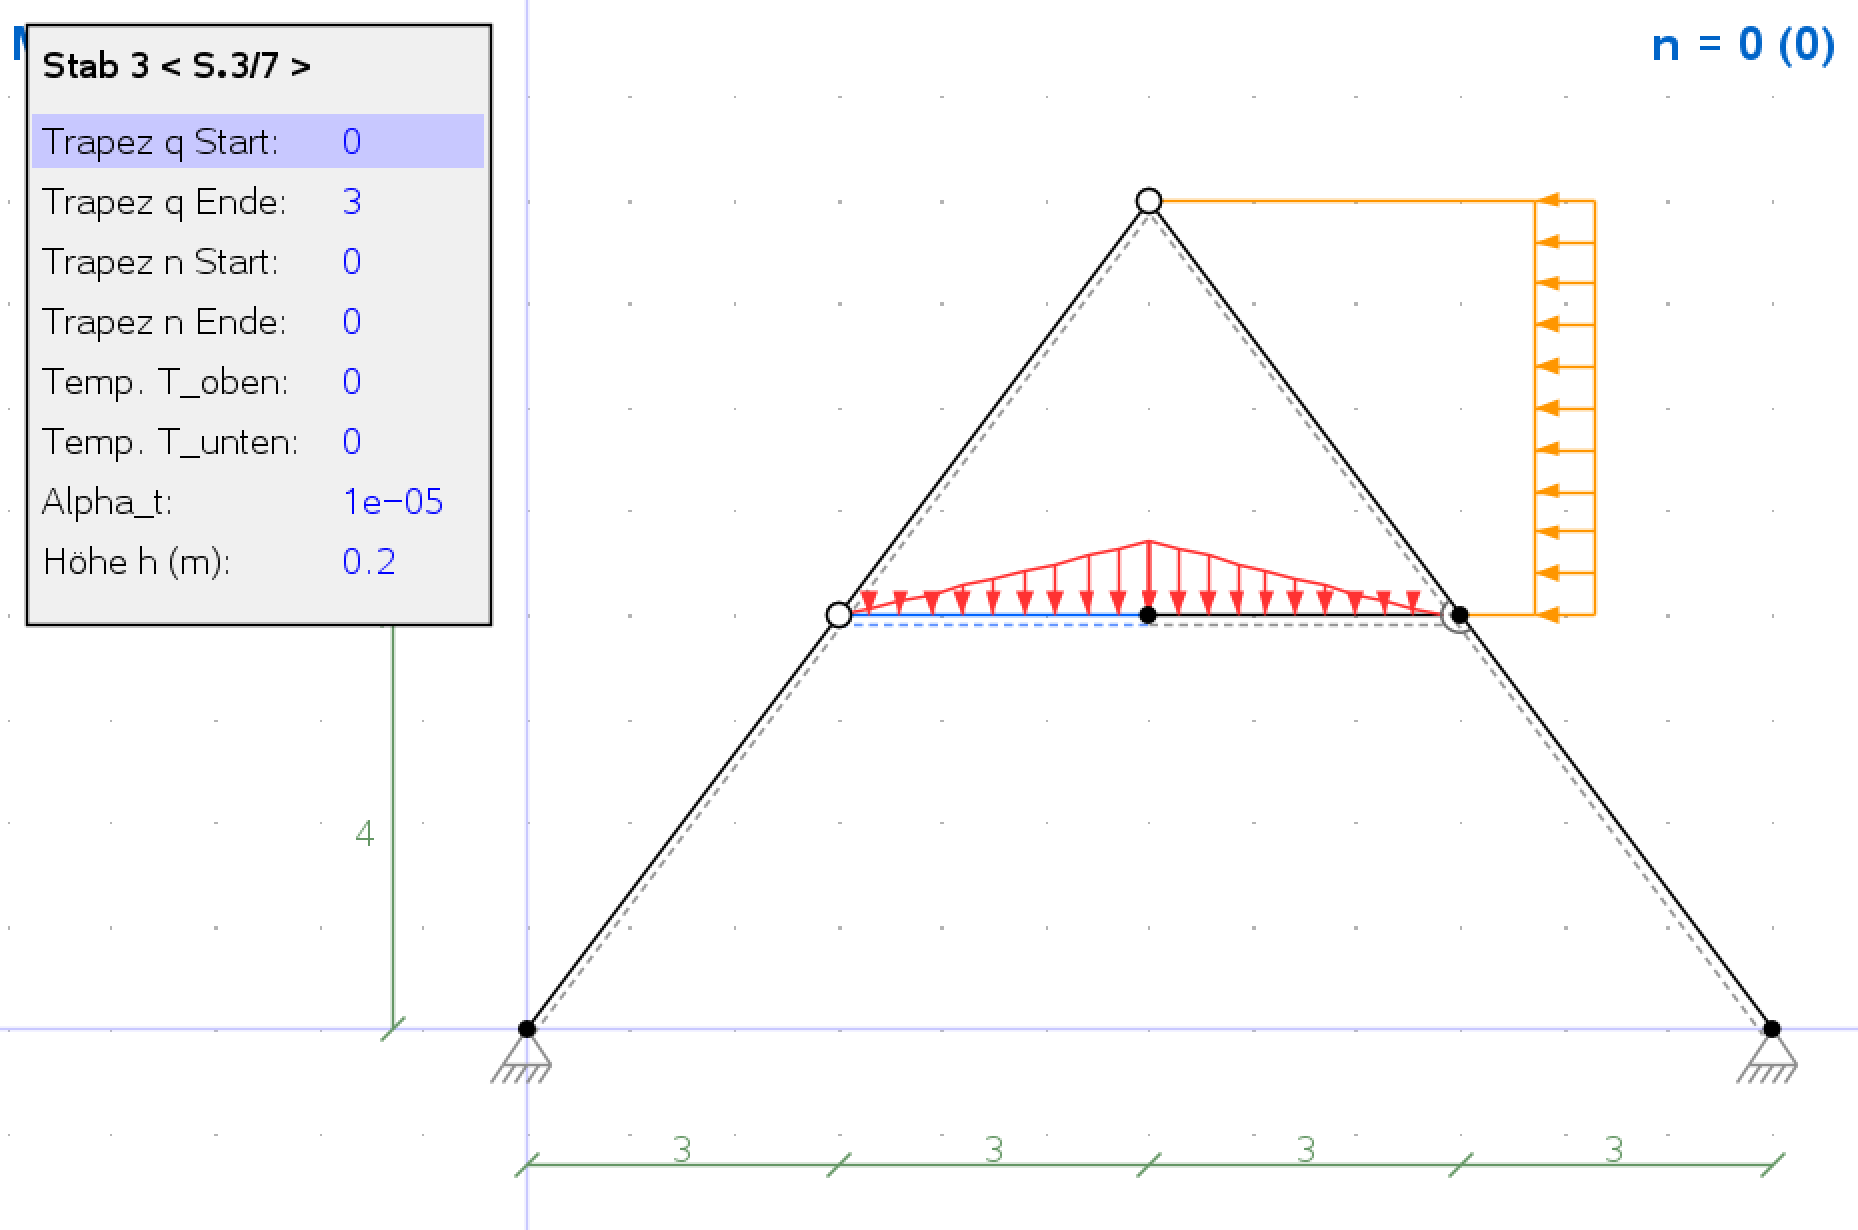
\includegraphics[width=\linewidth]{./fig/TM1/WiSe2122nr2_1.png}
        \caption{Trapezlast auf der linken Hälfte des Mittelstabs}
    \end{subfigure}
    \hfill
    \begin{subfigure}[t]{0.48\textwidth}
        \centering
        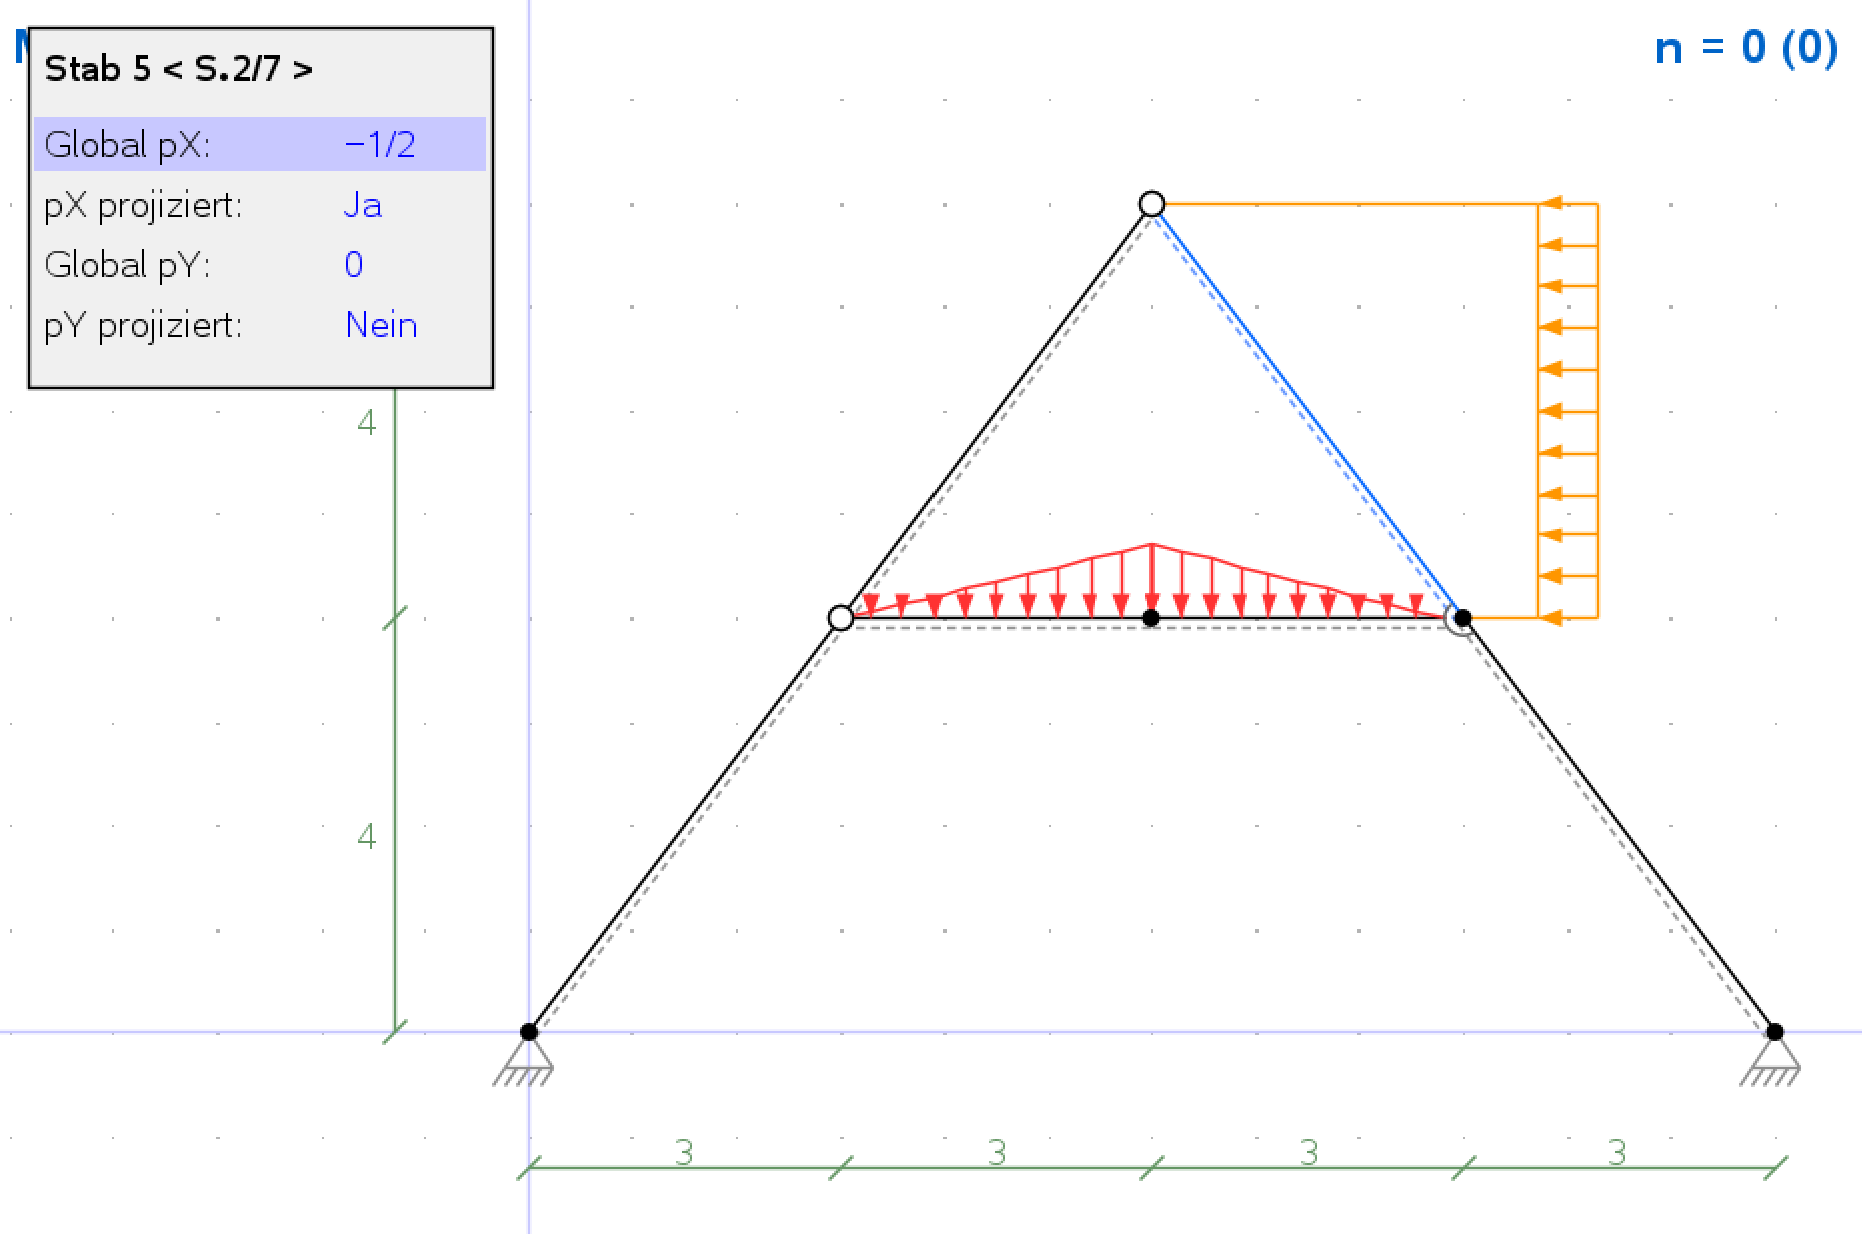
\includegraphics[width=\linewidth]{./fig/TM1/WiSe2122nr2_2.png}
        \caption{globale Streckenlast am oberen rechten Stab}
    \end{subfigure}
    \caption{WiSe~21/22, Nr.~2 im Programm}
    \label{fig:WiSe2122nr2_1}
\end{figure}

Den Stab in der Mitte müsst ihr im Programm teilen. Die Last auf ihm ist dreieckförmig mit der
Spitze in der Mitte, eine Trapezlast geht aber immer über einen ganzen Stab. Jede Hälfte bekommt
deshalb ihre eigene Trapezlast, die linke von $0$ auf $3$, die rechte von $3$ auf $0$
(Abb.~\ref{fig:WiSe2122nr2_1}a). Der neue Knoten in der Mitte bleibt biegesteif.

Die Streckenlast am schrägen Stab gebt ihr am einfachsten als globale Last ein
(Abb.~\ref{fig:WiSe2122nr2_1}b). In der Aufgabe ist sie auf die senkrechte Projektion des Stabes
bezogen, deshalb muss \emph{pX projiziert} auf \emph{Ja} stehen. Negativ ist sie, weil sie global
gesehen entgegen der $x$-Achse wirkt, also nach links.

Nach dem Berechnen könnt ihr das LGS, das zur Explosionsansicht (Abb.~\ref{fig:WiSe2122nr2_2})
gehört, über die zweite Seite des Obermenüs (\emph{LGS-Matrix}) in den Taschenrechner exportieren
(Abb.~\ref{fig:WiSe2122nr2_3}). Die Gleichungen stehen dann lesbar in \code{lgs}, die Lösung
bekommt ihr zum Beispiel mit \code{ggw\_x = ggw\_a$^{-1}$*ggw\_b}
(Abschnitt~\ref{sec:lgs-matrix}).

\begin{figure}[htbp]
    \centering
    \begin{subfigure}[t]{0.48\textwidth}
        \centering
        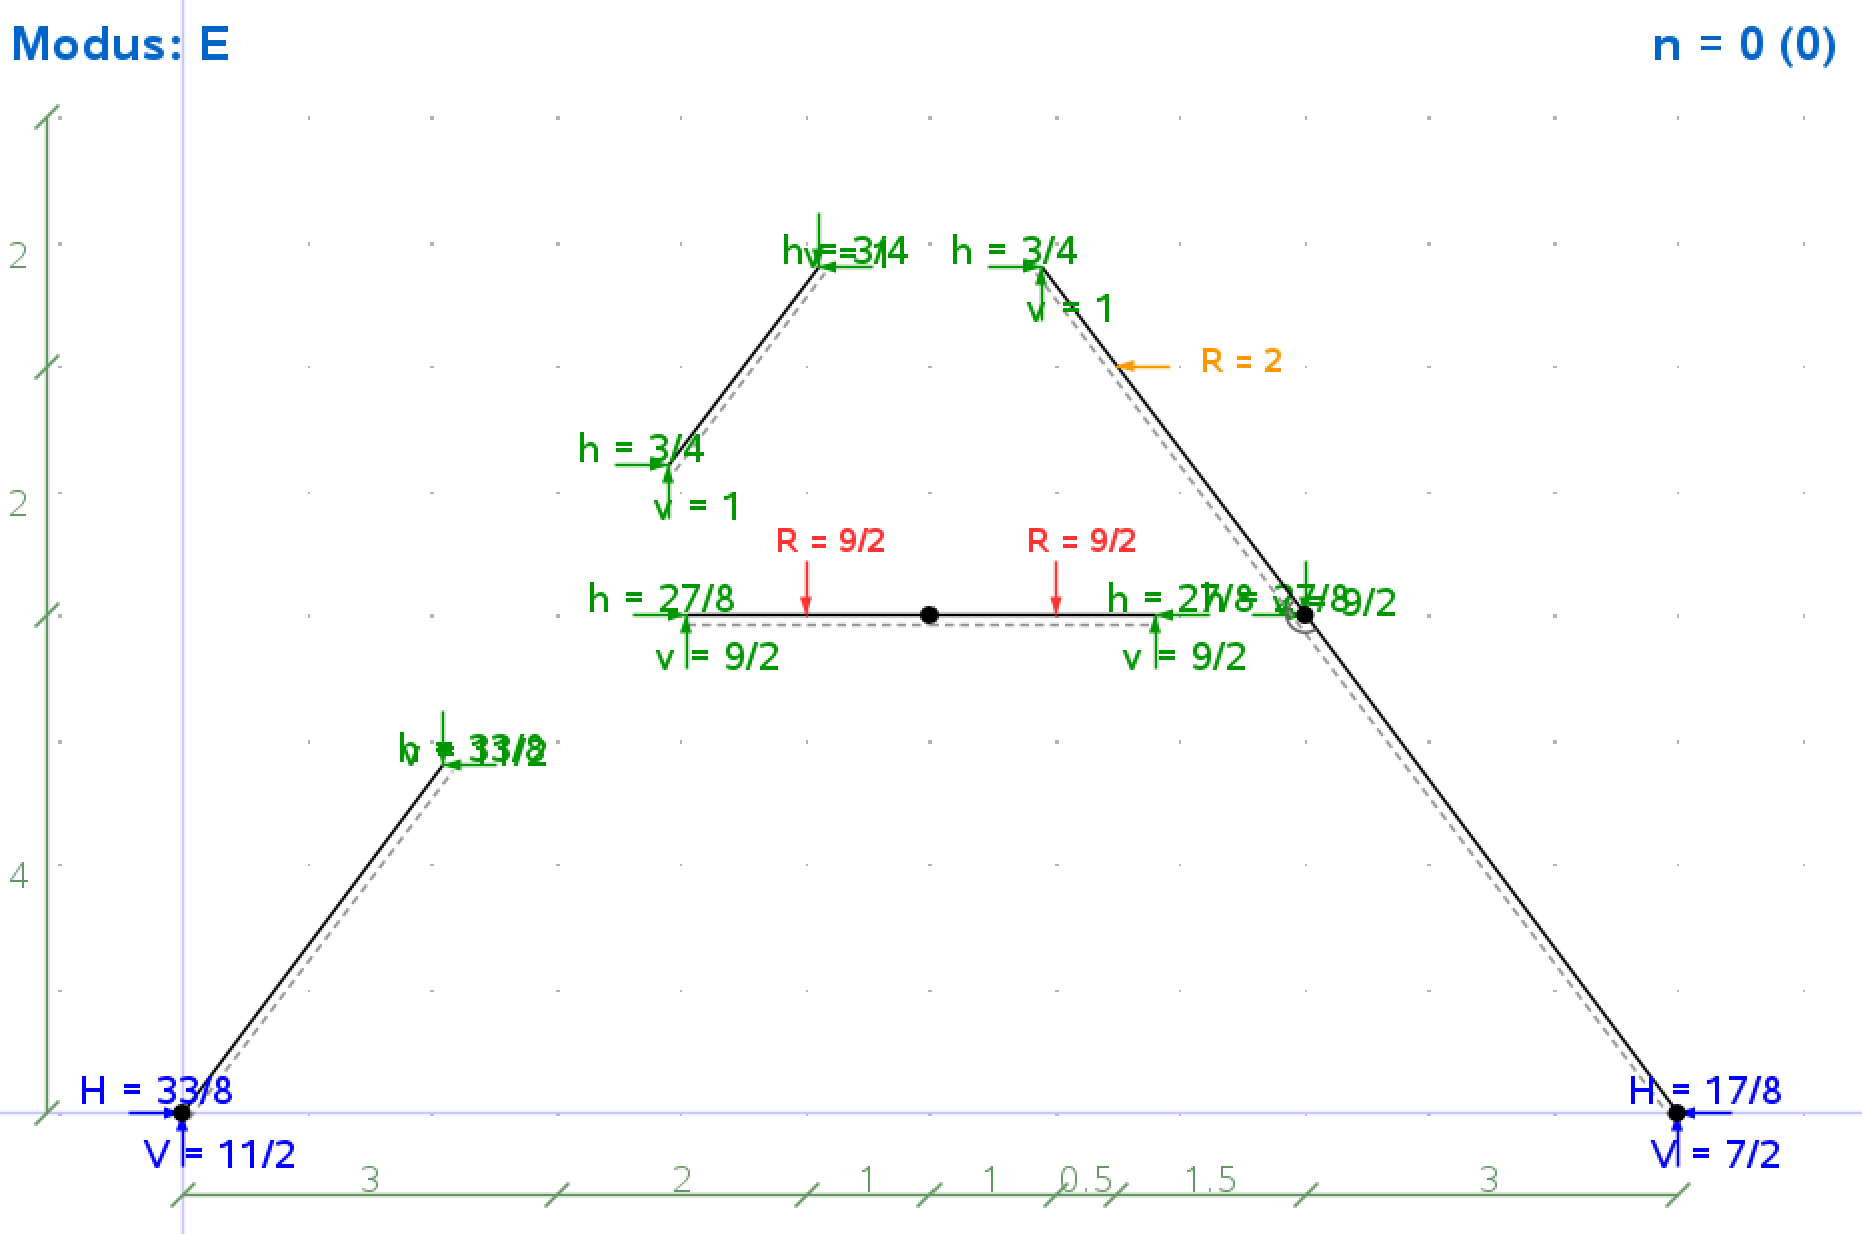
\includegraphics[width=\linewidth]{./fig/TM1/WiSe2122nr2_5.png}
        \caption{Seite~1: Ergebnisse in ihrer wirklichen Richtung}
    \end{subfigure}
    \hfill
    \begin{subfigure}[t]{0.48\textwidth}
        \centering
        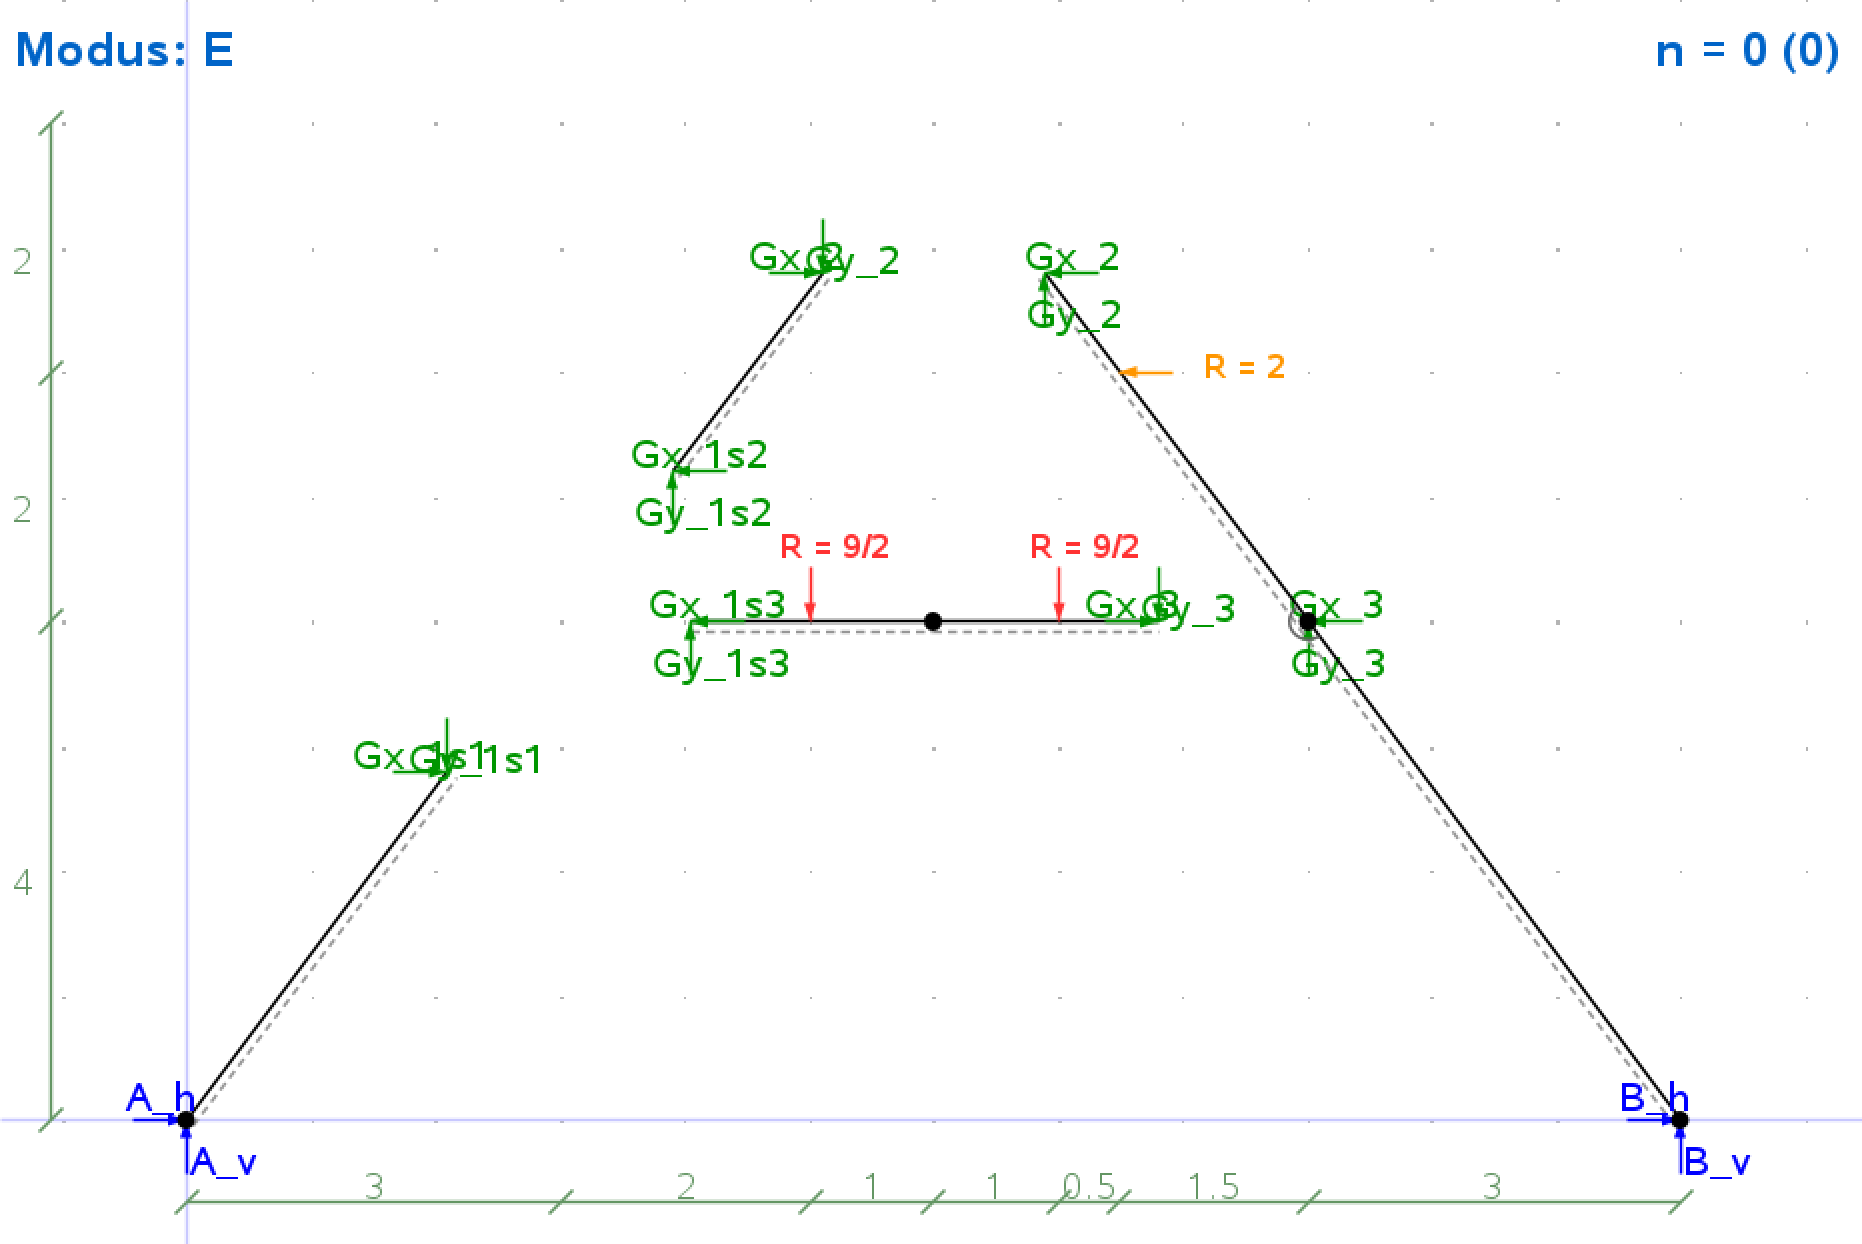
\includegraphics[width=\linewidth]{./fig/TM1/WiSe2122nr2_6.png}
        \caption{Seite~2: Unbekannte in positiver Richtung}
    \end{subfigure}
    \caption{WiSe~21/22, Nr.~2: Explosionsansicht (E-Modus)}
    \label{fig:WiSe2122nr2_2}
\end{figure}

\begin{figure}[htbp]
    \centering
    \begin{subfigure}[t]{0.48\textwidth}
        \centering
        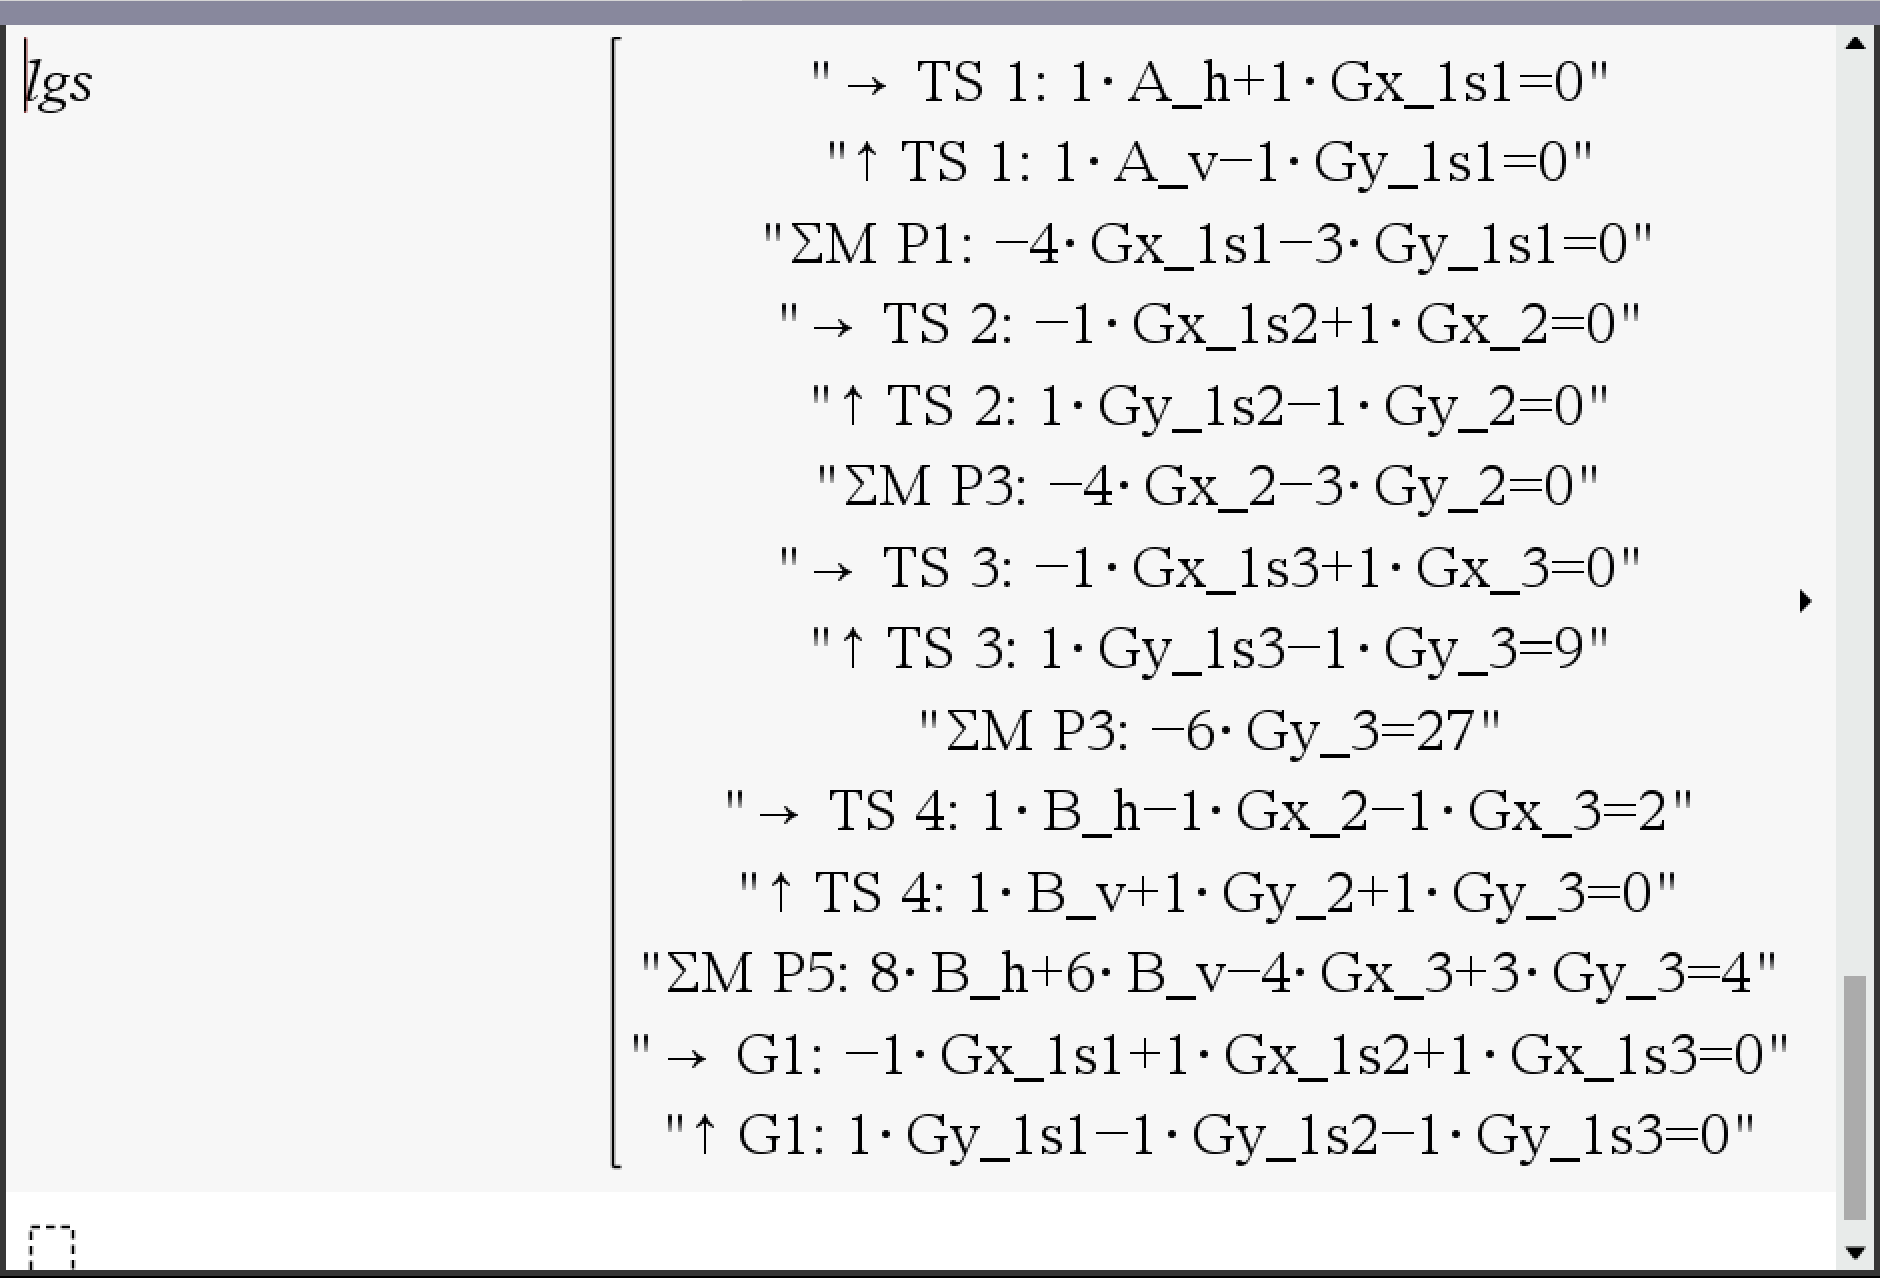
\includegraphics[width=\linewidth]{./fig/TM1/WiSe2122nr2_3.png}
        \caption{exportierte Gleichungen \code{lgs}}
    \end{subfigure}
    \hfill
    \begin{subfigure}[t]{0.48\textwidth}
        \centering
        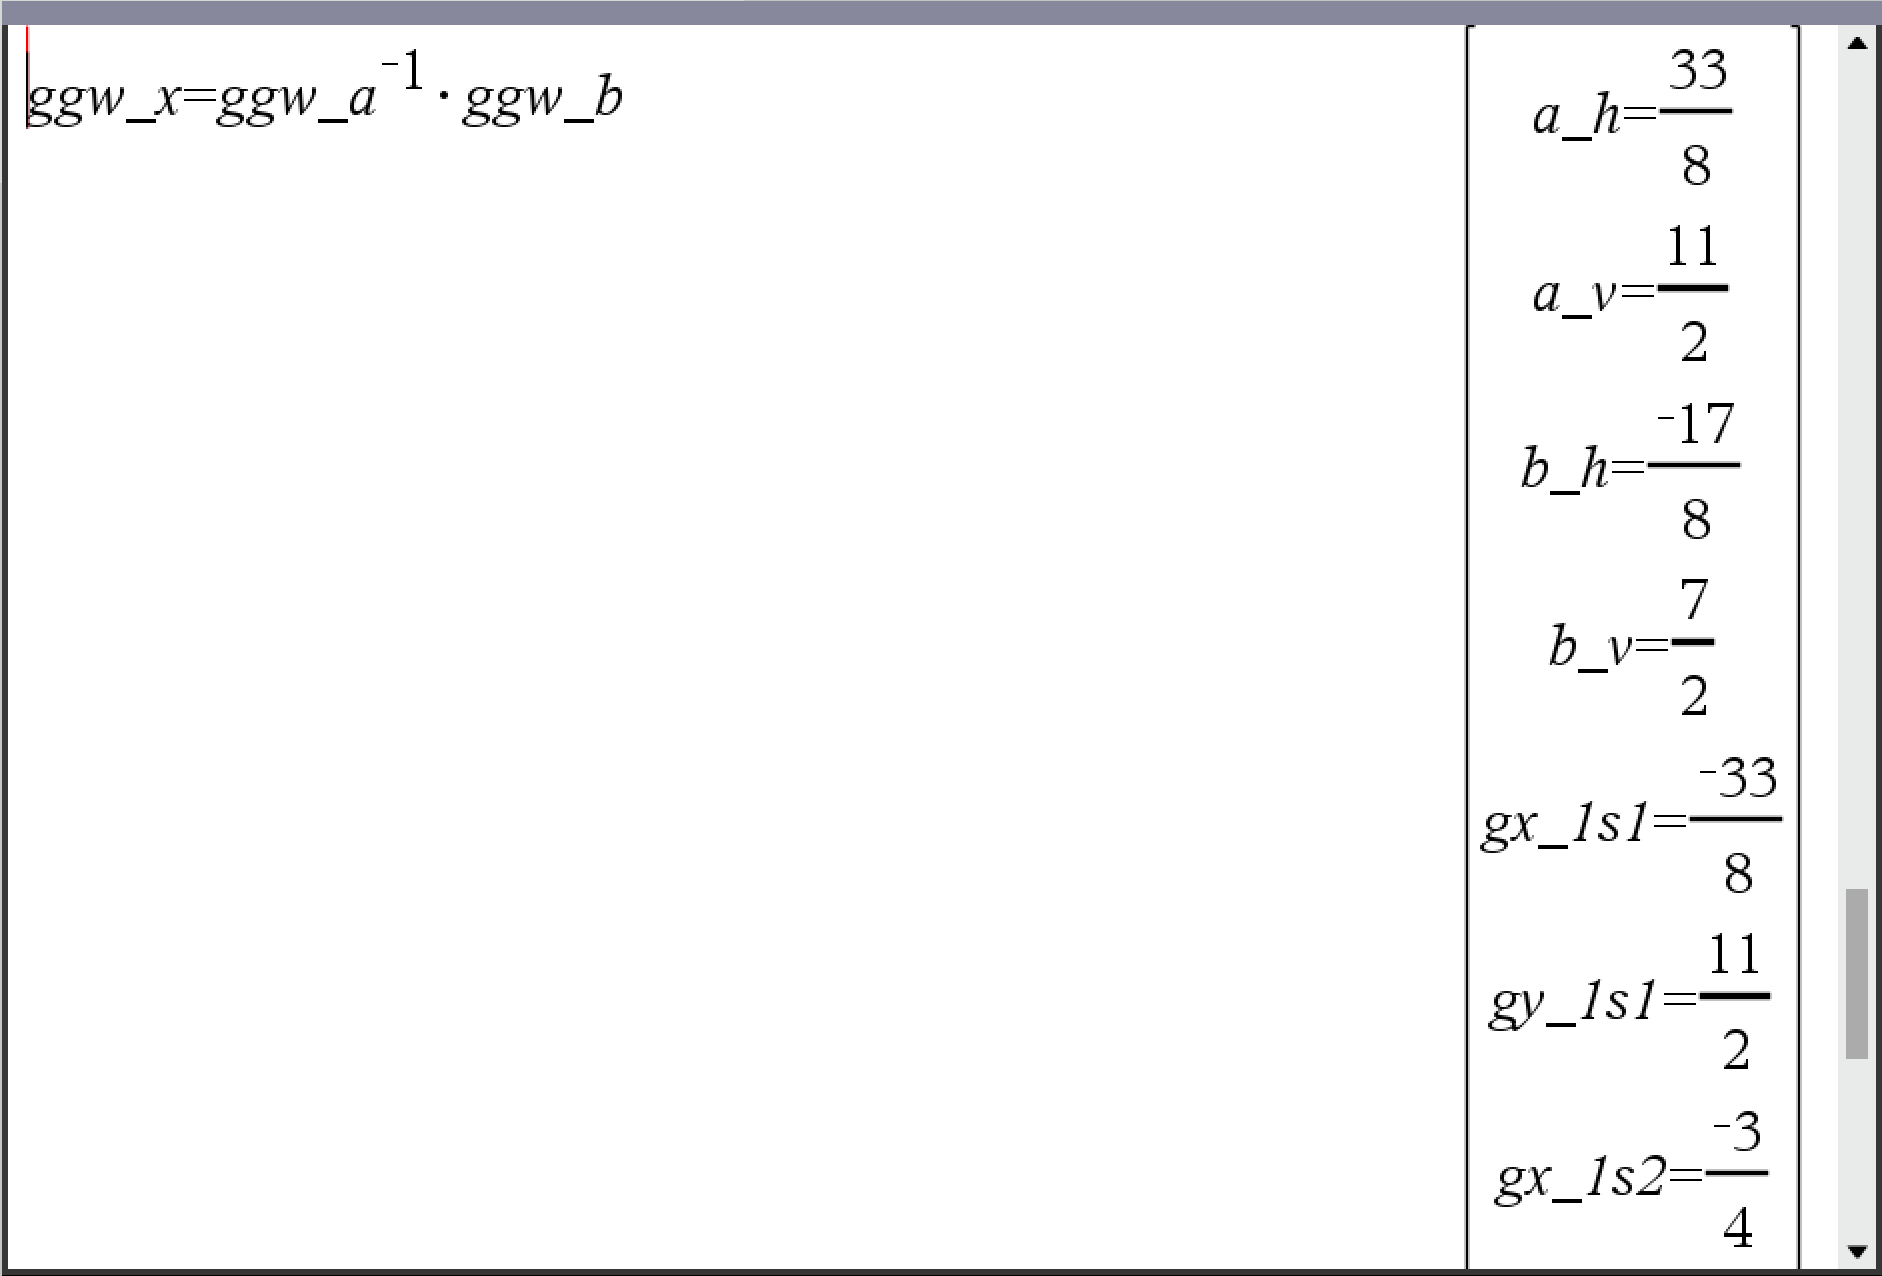
\includegraphics[width=\linewidth]{./fig/TM1/WiSe2122mr2_4.png}
        \caption{Lösung mit \code{ggw\_x}}
    \end{subfigure}
    \caption{WiSe~21/22, Nr.~2: exportiertes LGS}
    \label{fig:WiSe2122nr2_3}
\end{figure}

Die Explosionsansicht kann manchmal etwas unübersichtlich sein. Wenn ihr nah genug heranzoomt,
sollte aber trotzdem alles erkennbar sein. Die Ergebnisse müsst ihr natürlich nicht in dieser
Vektorform aufschreiben, nur ihr Inhalt zählt.

An dieser Stelle will ich anmerken, dass meist nur bei Systemen mit einem geschlossenen Ring wie
diesem nach allen Gelenk- und Auflagerkräften gefragt wird. Bei offenen Systemen ohne Ring wird oft
nur nach den Auflagerkräften gefragt. Das exportierte LGS liefert dann zwar auch die richtige Lösung, ist aber
meist mehr, als ihr braucht. Den Punkt, um den das Programm die Momentensumme eines Teilsystems
bildet, seht ihr, wenn ihr in der Explosionsansicht mit der Maus über das Teilsystem fahrt
(\emph{Hover}).

Die Zustandslinien, also die Verläufe der Schnittgrößen, zeichnet euch das Programm mit den Tasten
\taste{n}, \taste{q} und \taste{m}, die könnt ihr einfach abzeichnen. Falls ihr Randwerte schlecht
erkennt, fahrt mit der Maus über den jeweiligen Stab, dann zeigt das Programm nur noch diesen Stab
mit seinen Randwerten an.

\subsubsection{Qualitavtive Verläufe im symbolischen Modus (Nr.~4)}

Um meinen den oben genannten Punkt zum symbolischen Modus zu verdeutlichen will ich hier kurz auf Teilaufgabe b) eingehen.
Das System und der Querkraftverlauf sind in Abbildung~\ref{fig:TM1WiSe2122Nr4} dargestellt.

\begin{figure}[htbp]
    \centering
    \begin{subfigure}[t]{0.48\textwidth}
        \centering
        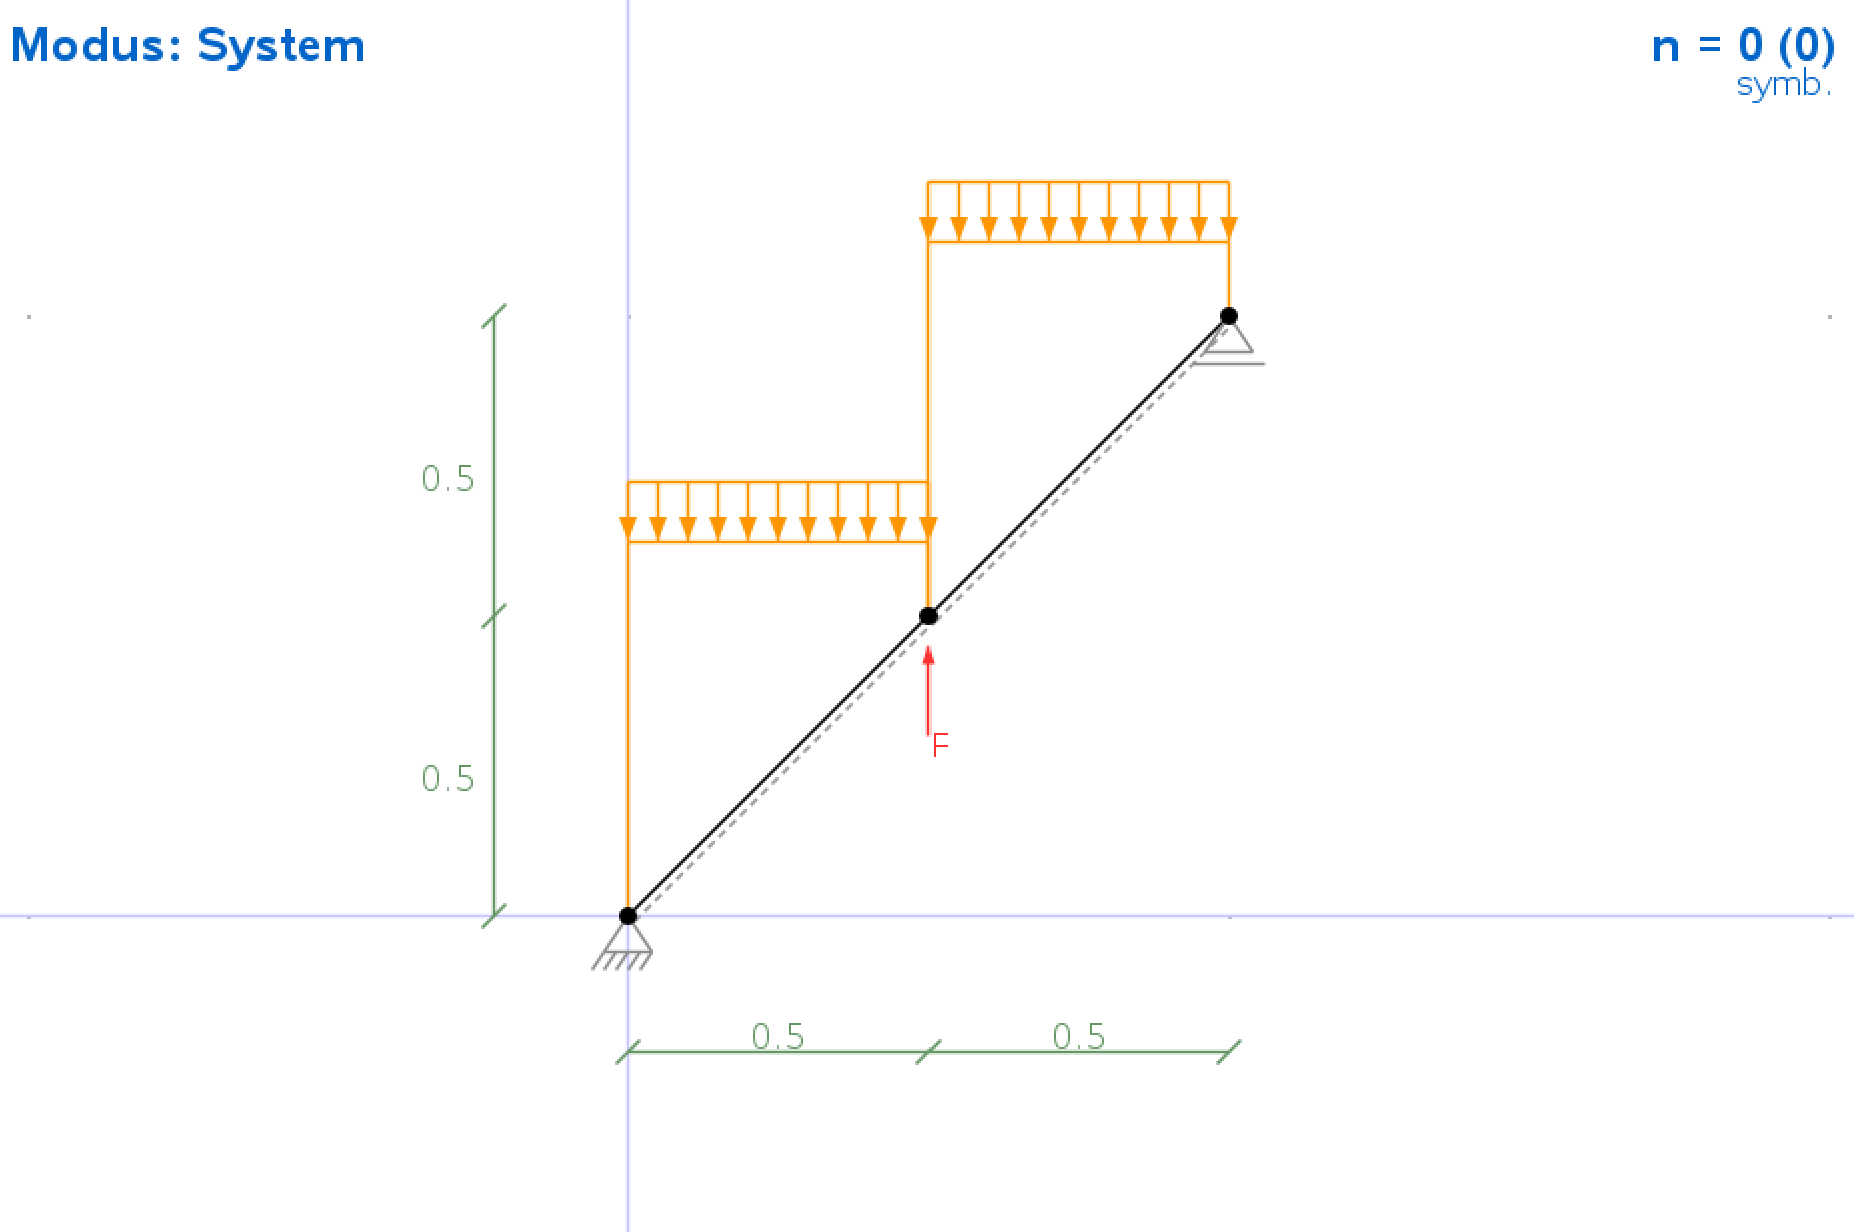
\includegraphics[width=\linewidth]{./fig/TM1/WiSe2122nr4_1.png}
        \caption{System}
    \end{subfigure}
    \hfill
    \begin{subfigure}[t]{0.48\textwidth}
        \centering
        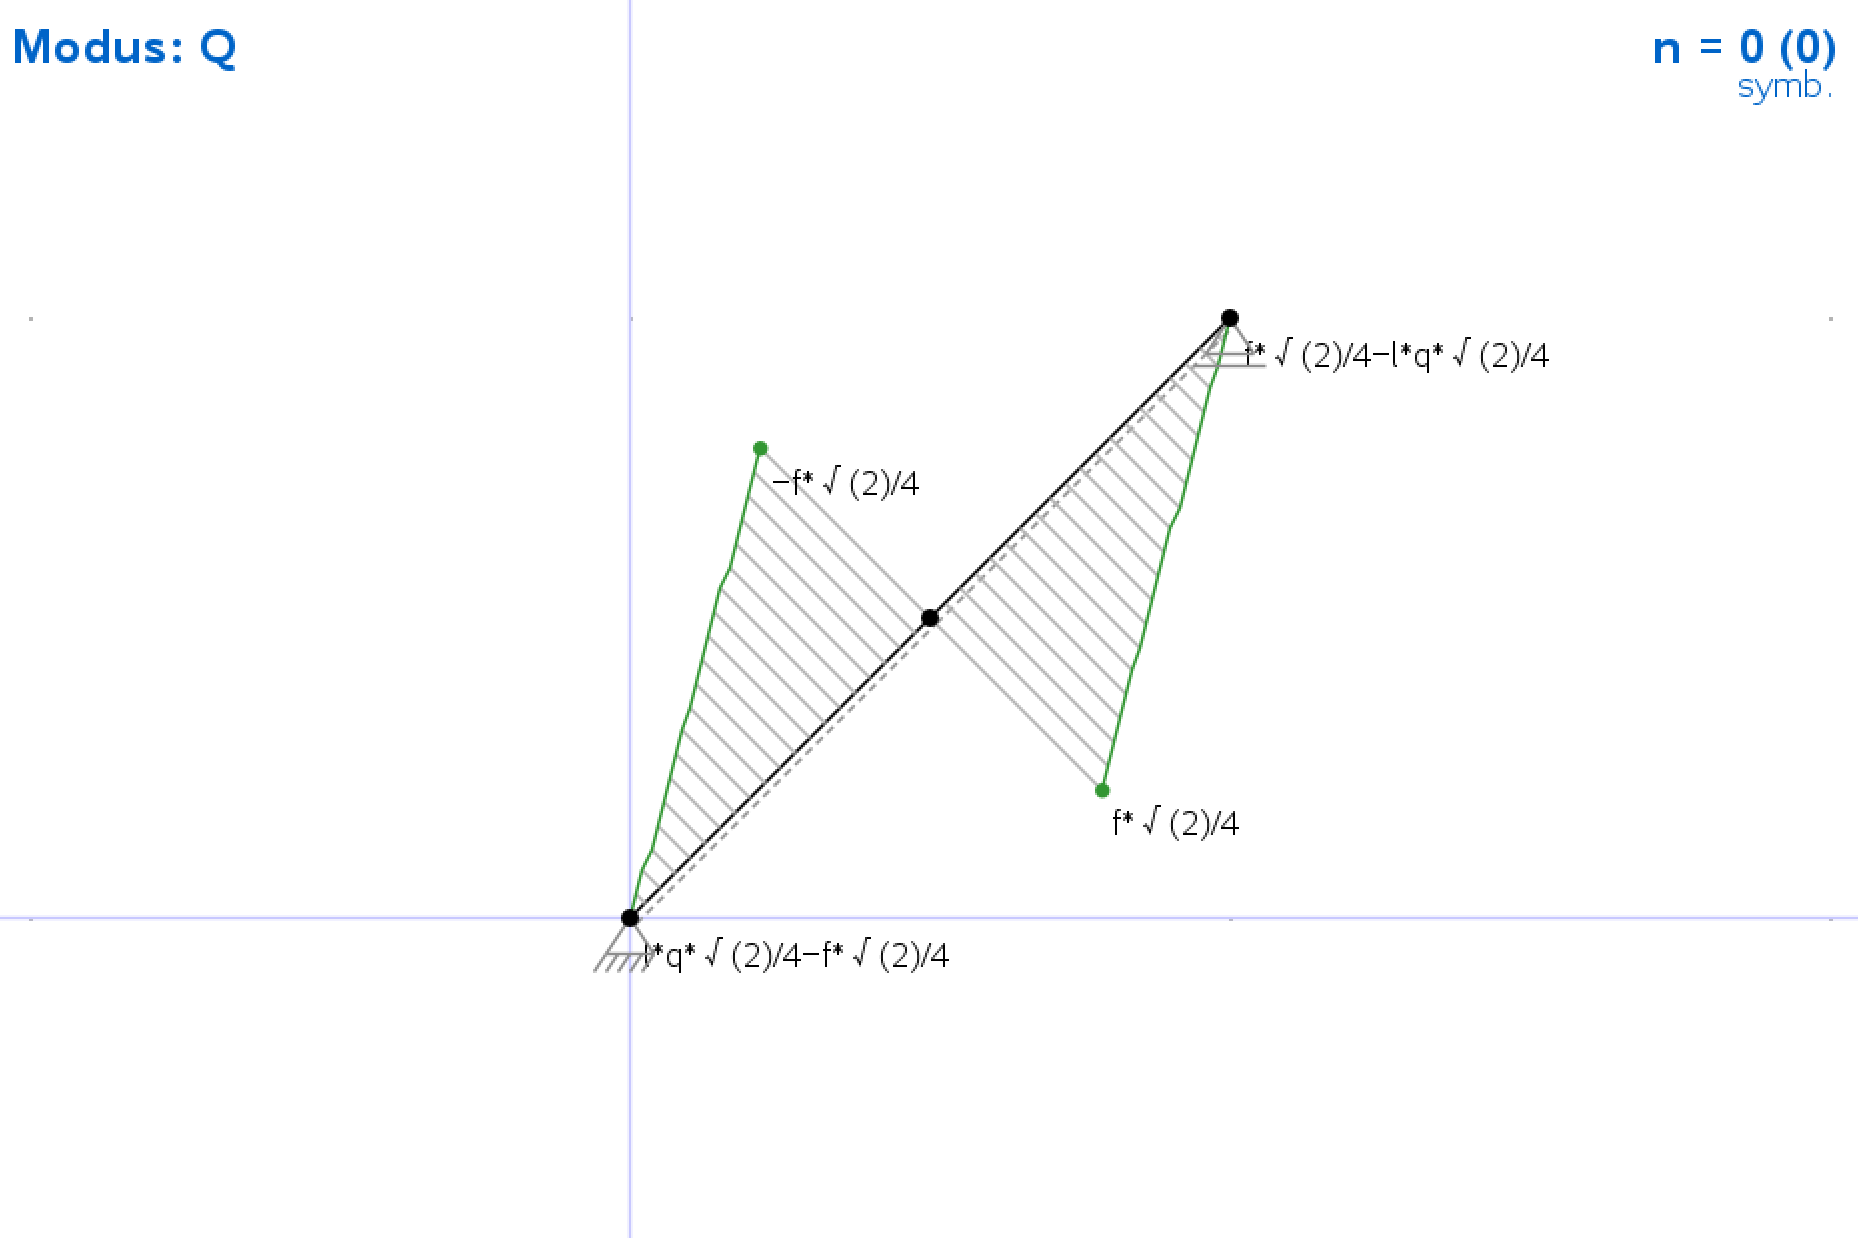
\includegraphics[width=\linewidth]{./fig/TM1/WiSe2122nr4_2.png}
        \caption{Querkraftverlauf}
    \end{subfigure}
    \caption{WiSe~21/22, Nr.~4}
    \label{fig:TM1WiSe2122Nr4}
\end{figure}

Im Querkraft verlauf sieht es so aus, als ob diese an den Auflagern null wird. Wenn man sich die Beschriftung der Randwerte 
anschaut wird jedoch klar, dass ist nur der Fall, wenn $q\cdot l=F$ bzw. $q\cdot a=F$ gilt. Das ist eben genau die Annhame des Programms,
um überhaupt irgendeinen Verlauf zeichnen zu können.
Die Aufgabe gibt aber unten vor: $F>q\cdot a$. Damit wird die Qerkraft am linekn Ende negativ und am rechten Ende positiv.
Die Verläufe von symbolische Berechnungen solltet ihr also \textbf{nie} einfach blind abzeichnen.

\subsection{PvV (Nr.~3)}

Zum PvV gibt es eigentlich nicht viel zu sagen. System zeichnen, \taste{v} drücken, Bindung wählen, abzeichnen,
dann exportieren und aufschreiben. 


\begin{figure}[htbp]
    \centering
    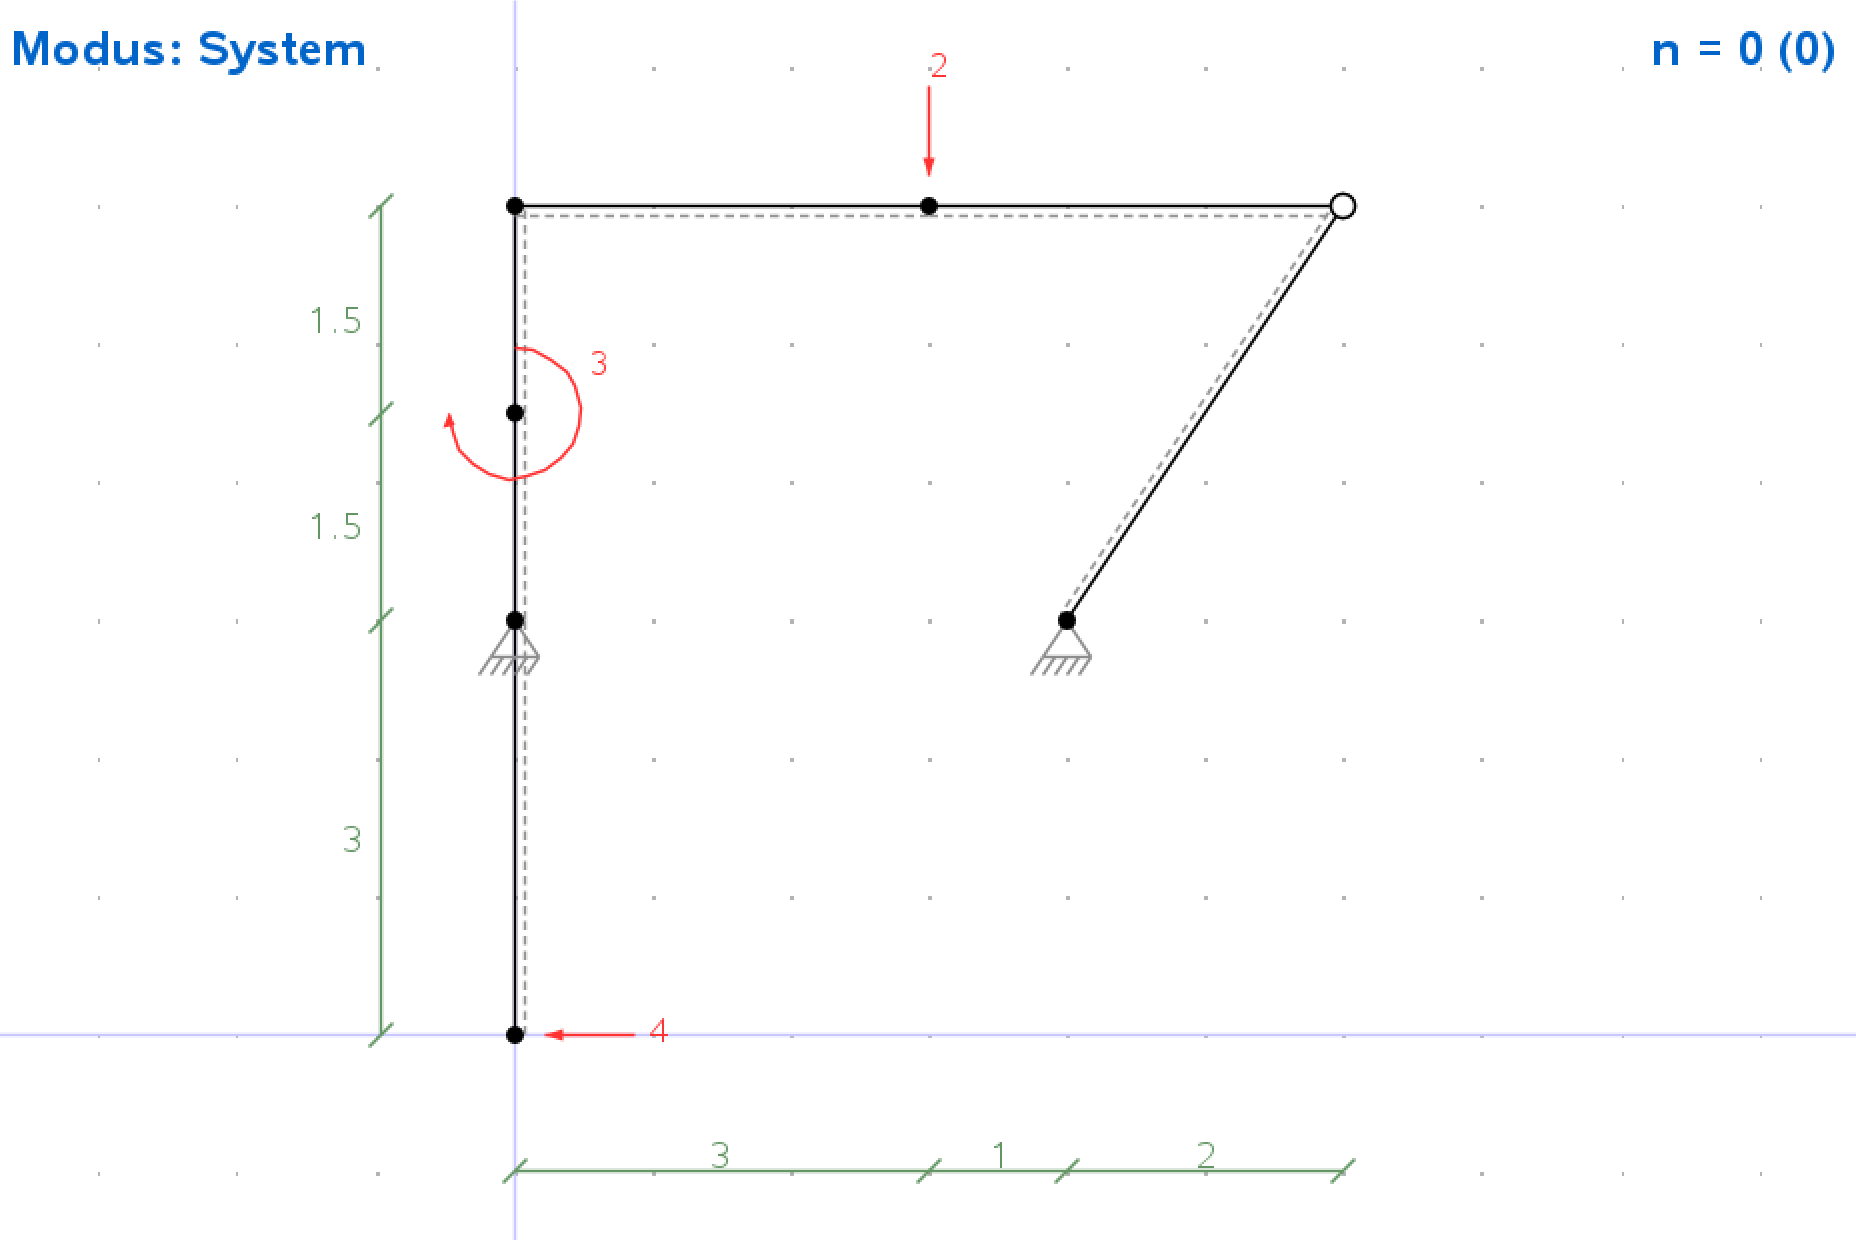
\includegraphics[width=0.5\linewidth]{./fig/TM1/WiSe2122nr3_1.png}
    \caption{TM1 WiSe~21/22, Nr.~3 im Programm}
    \label{fig:TM1WiSe2122Nr3_1}
\end{figure}

\begin{figure}[htbp]
    \centering
    \begin{subfigure}[t]{0.48\textwidth}
        \centering
        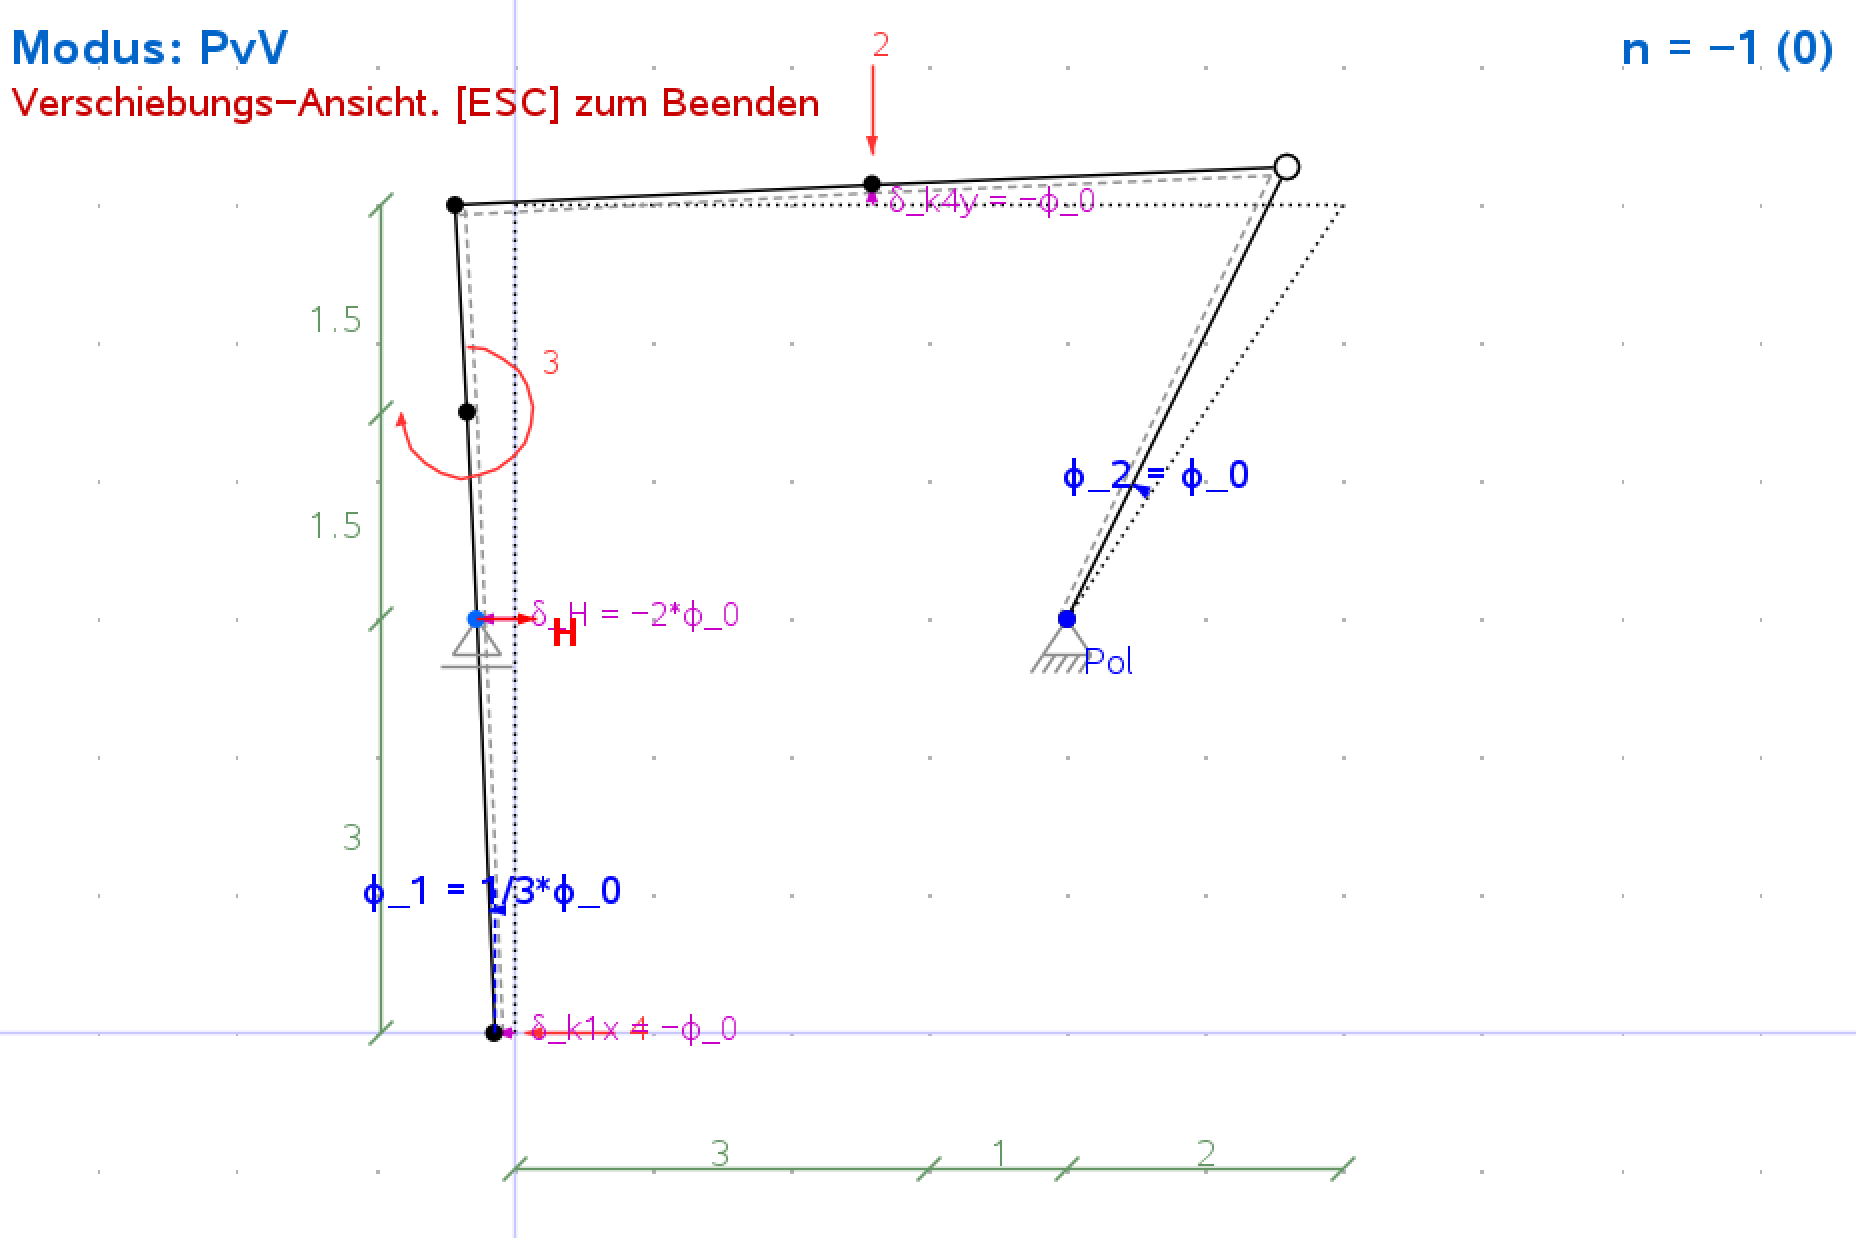
\includegraphics[width=\linewidth]{./fig/TM1/WiSe2122nr3_2.png}
        \caption{Verschiebungsfigur für $A_H$}
    \end{subfigure}
    \hfill
    \begin{subfigure}[t]{0.48\textwidth}
        \centering
        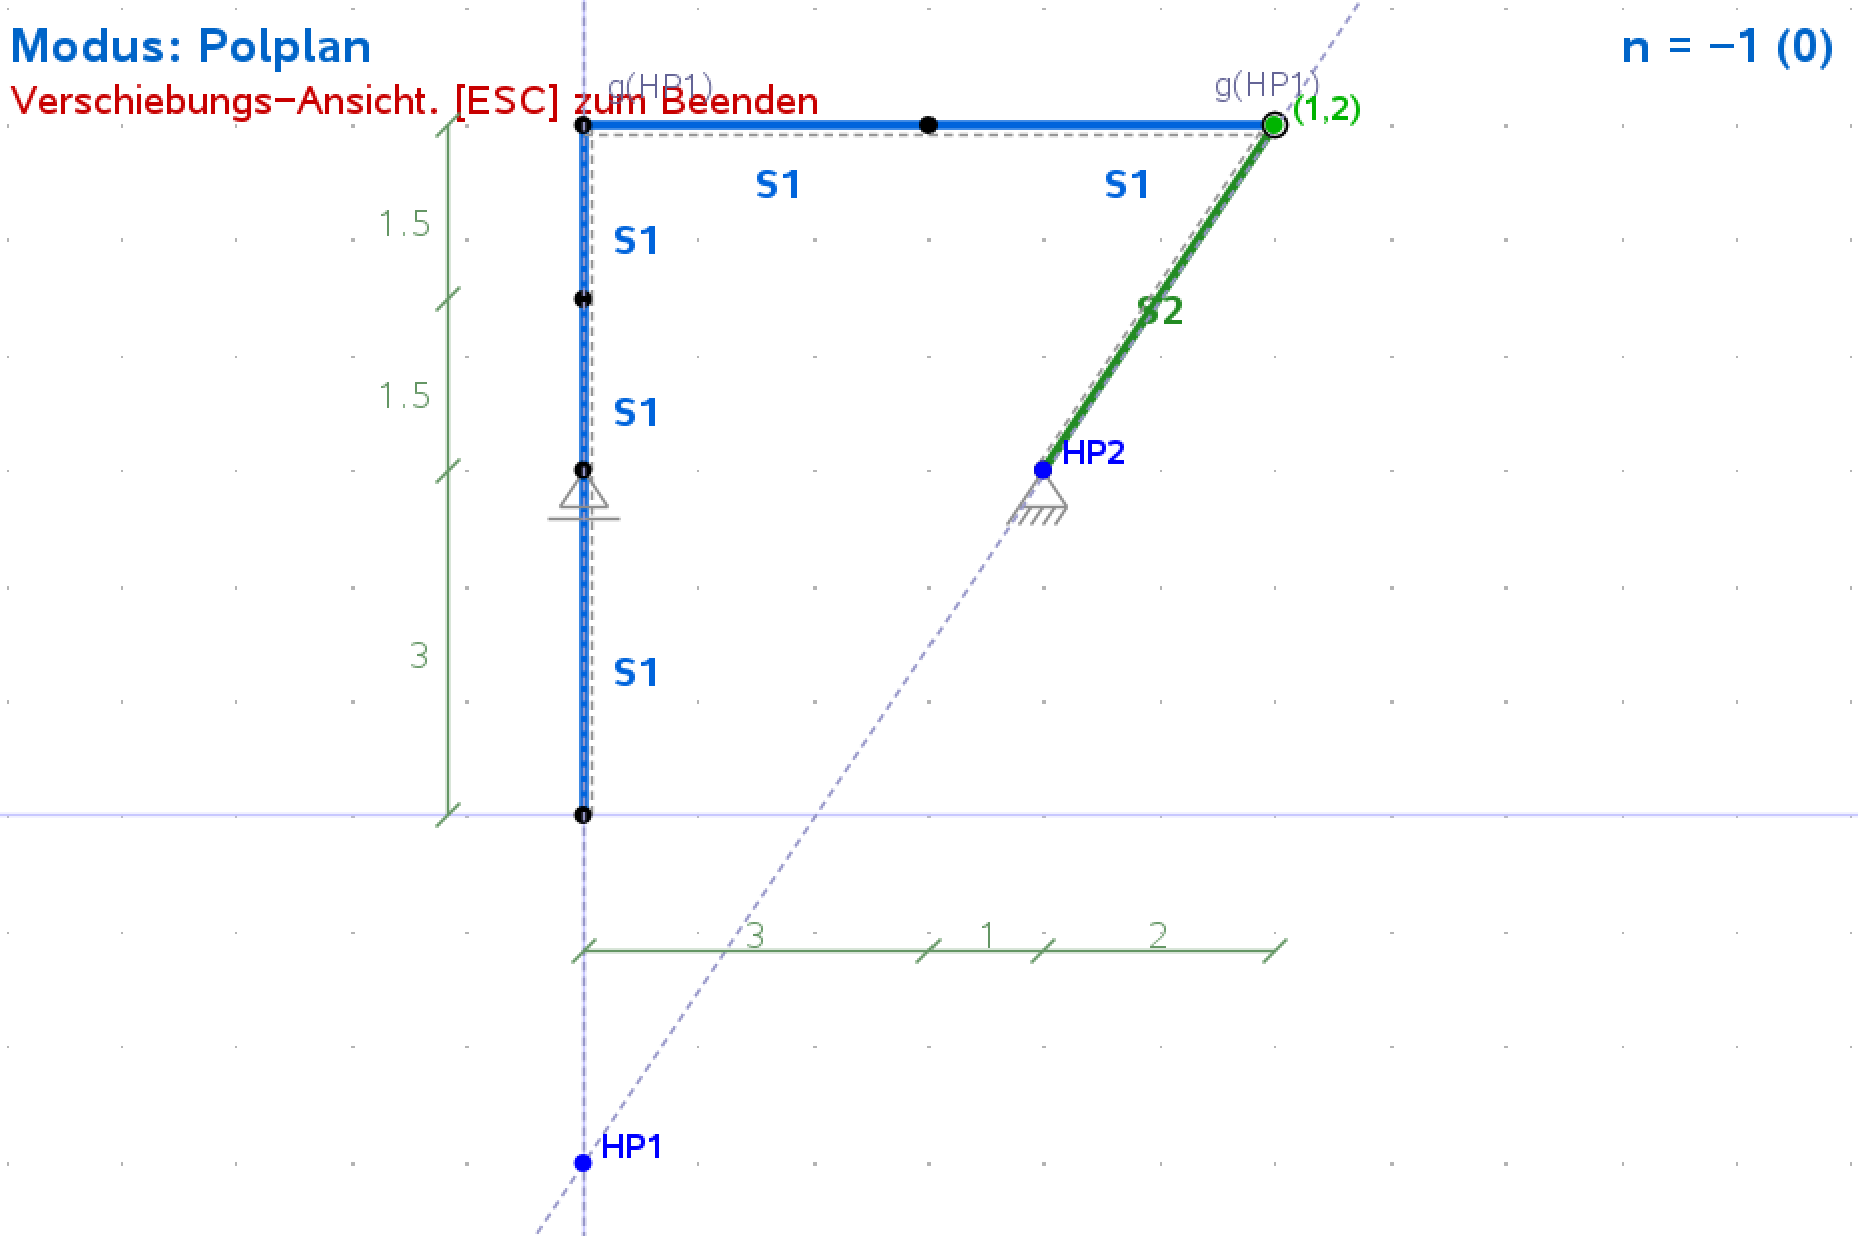
\includegraphics[width=\linewidth]{./fig/TM1/WiSe2122nr3_3.png}
        \caption{Polplan für $A_H$}
    \end{subfigure}
    \caption{WiSe~21/22, Nr.~3: $A_H$}
    \label{fig:TM1WiSe2122Nr3_2}
\end{figure}

\begin{figure}[htbp]
    \centering
    \begin{subfigure}[t]{0.48\textwidth}
        \centering
        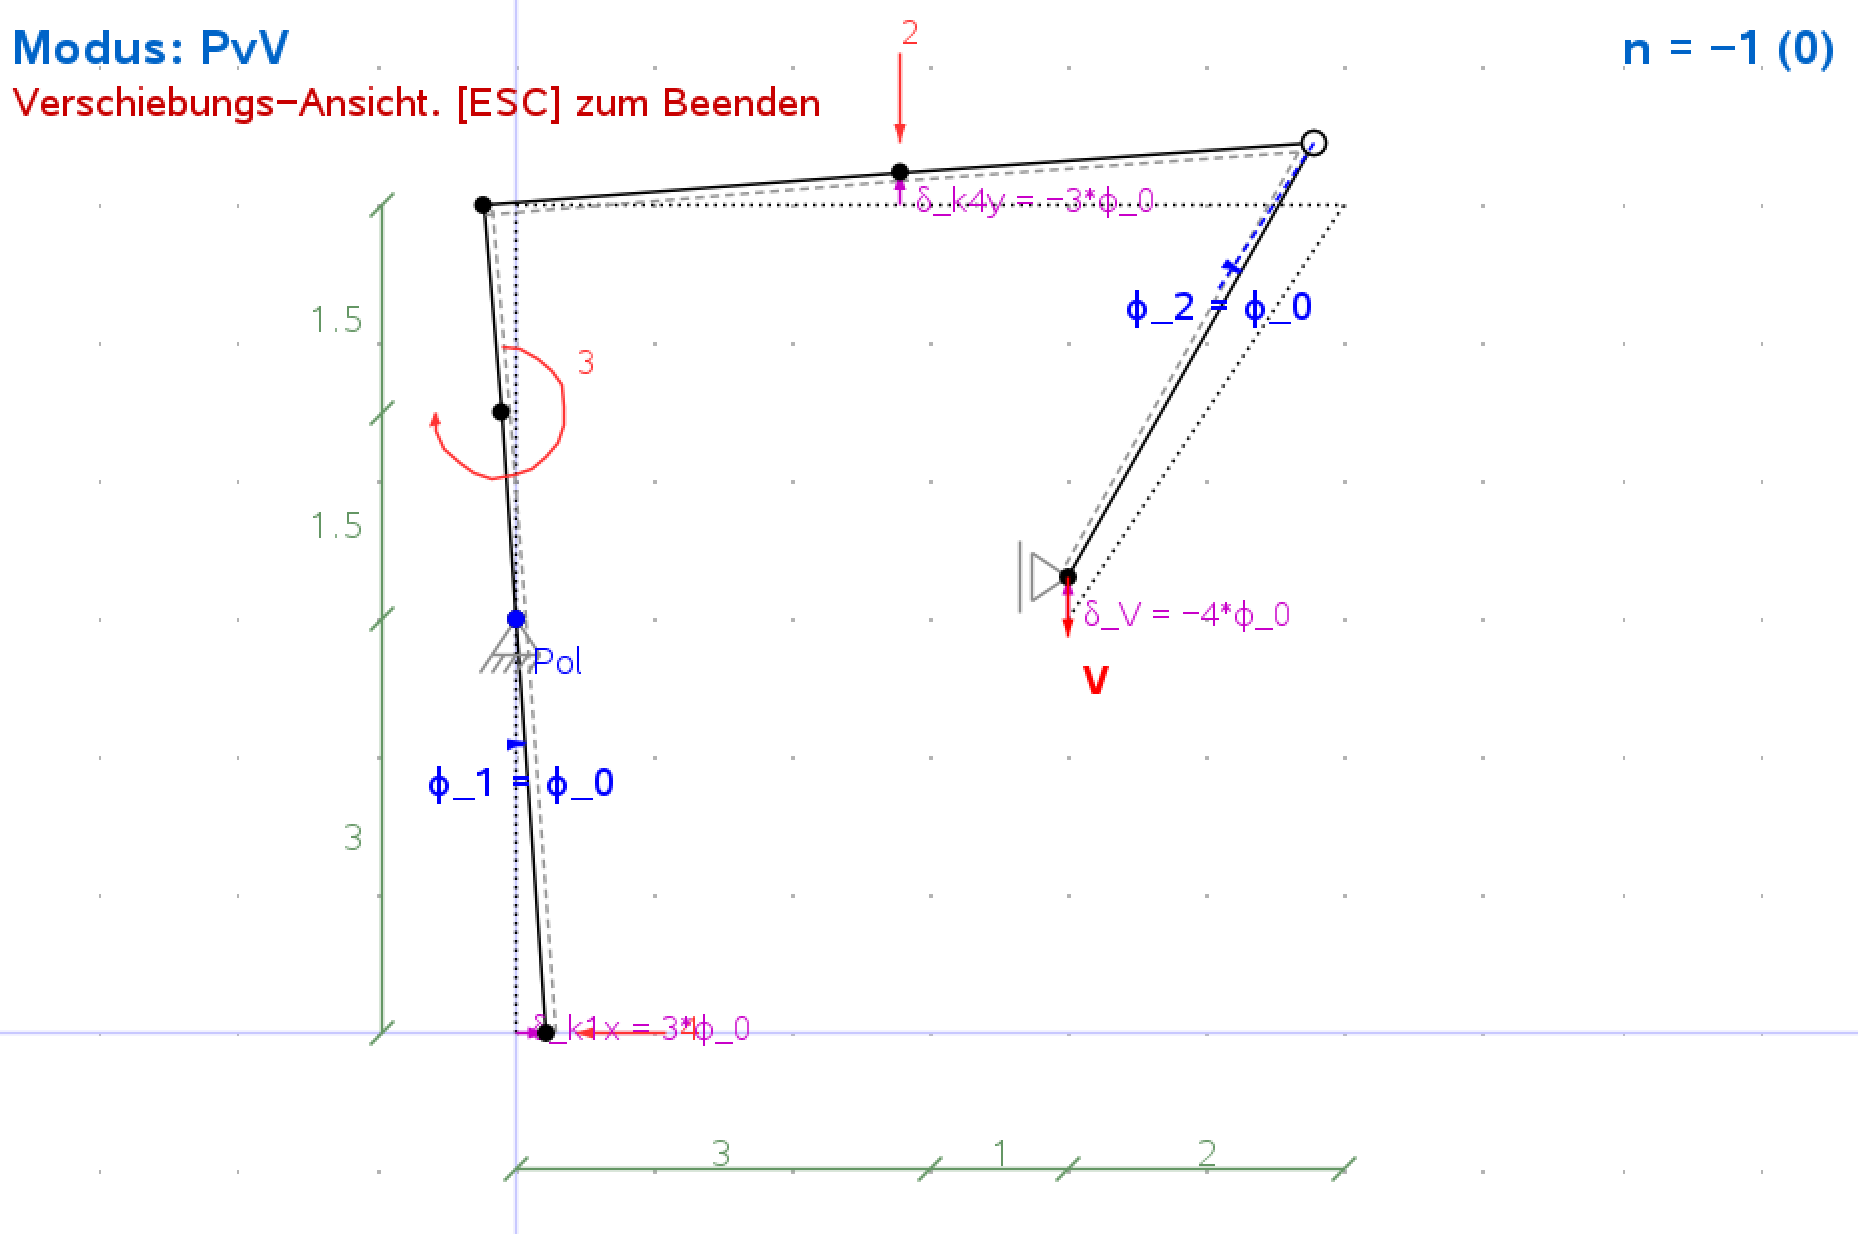
\includegraphics[width=\linewidth]{./fig/TM1/WiSe2122nr3_4.png}
        \caption{Verschiebungsfigur für $B_V$}
    \end{subfigure}
    \hfill
    \begin{subfigure}[t]{0.48\textwidth}
        \centering
        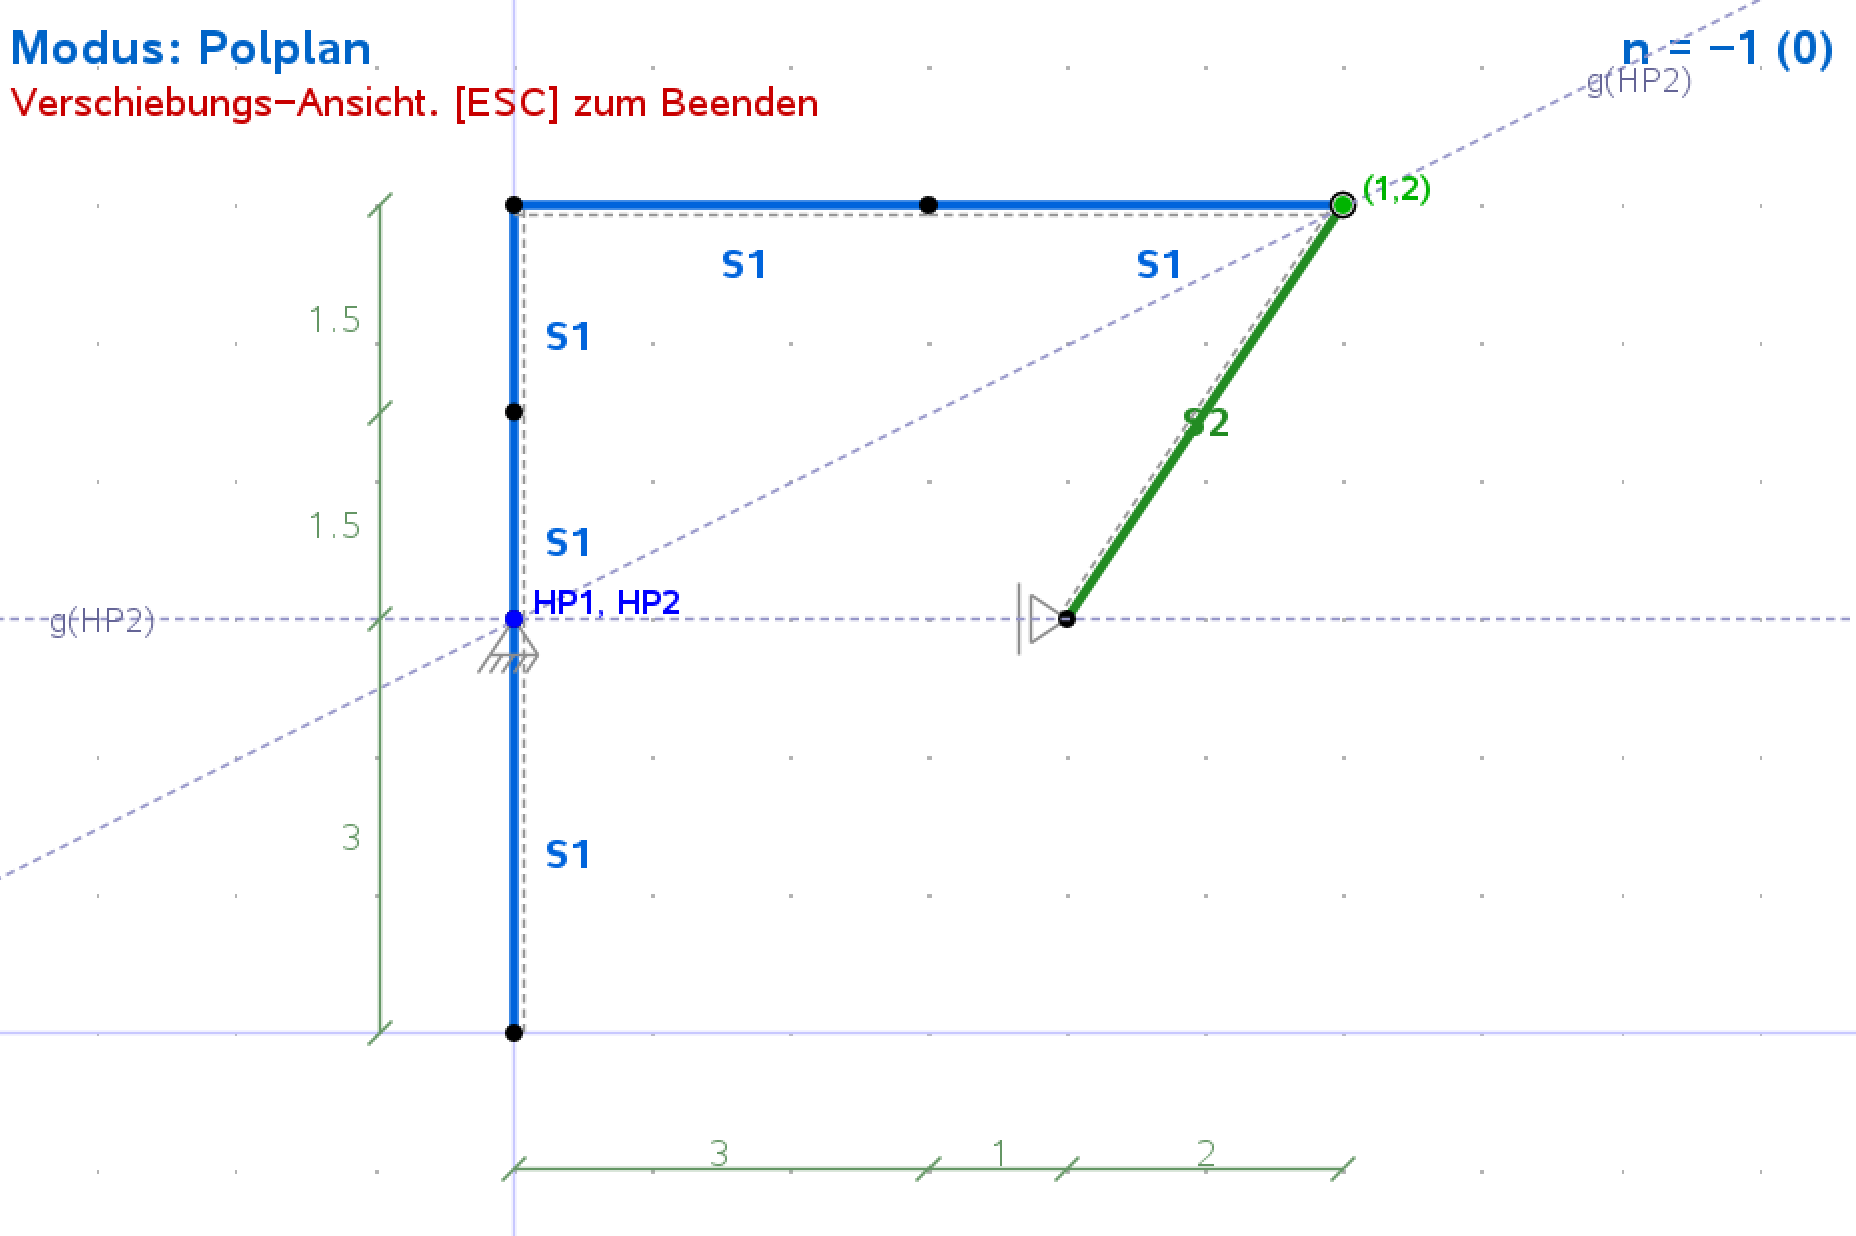
\includegraphics[width=\linewidth]{./fig/TM1/WiSe2122nr3_5.png}
        \caption{Polplan für $B_V$}
    \end{subfigure}
    \caption{WiSe~21/22, Nr.~3: $B_V$}
    \label{fig:TM1WiSe2122Nr3_3}
\end{figure}

Die Zeilen der Matrizen \code{pvv\_kin} und \code{pvv\_pol} (Abb.~\ref{fig:TM1WiSe2122Nr3_4})
sind als Gleichungskette zu lesen. Hier gilt also z.B. $\delta_{k1x}= -3\cdot\varphi_1=-\varphi_0$, oder 
$\delta x_{p12}= -9\cdot\varphi_1=-3\varphi_2$. Mit diesen Gleichungen lässt sich aus \code{w\_eq1} \code{w\_eq2} bauen.
Diese gleichung lässt sich dann entweder von hand oder mit dem Taschenrechner nach der gesuchten Größe auflösen.

\begin{figure}[htbp]
    \centering
    \begin{subfigure}[t]{0.48\textwidth}
        \centering
        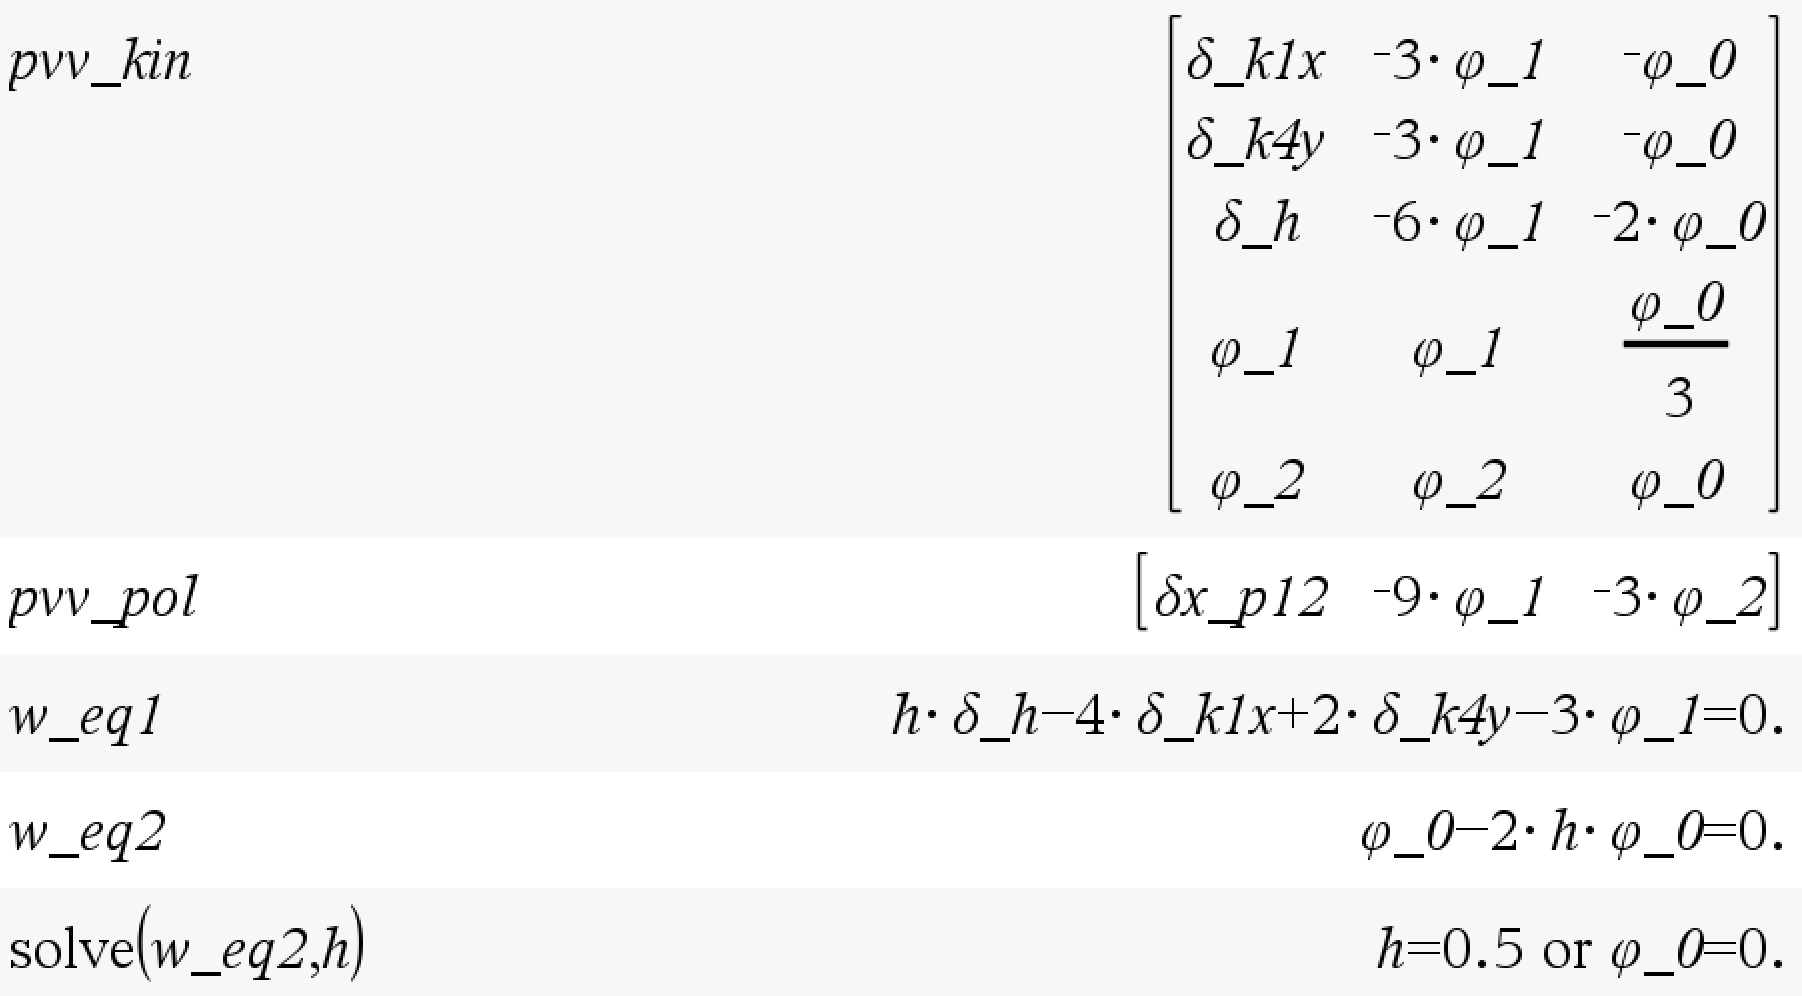
\includegraphics[width=\linewidth]{./fig/TM1/WiSe2122nr3_6.png}
        \caption{Rechnung für $A_H$}
    \end{subfigure}
    \hfill
    \begin{subfigure}[t]{0.48\textwidth}
        \centering
        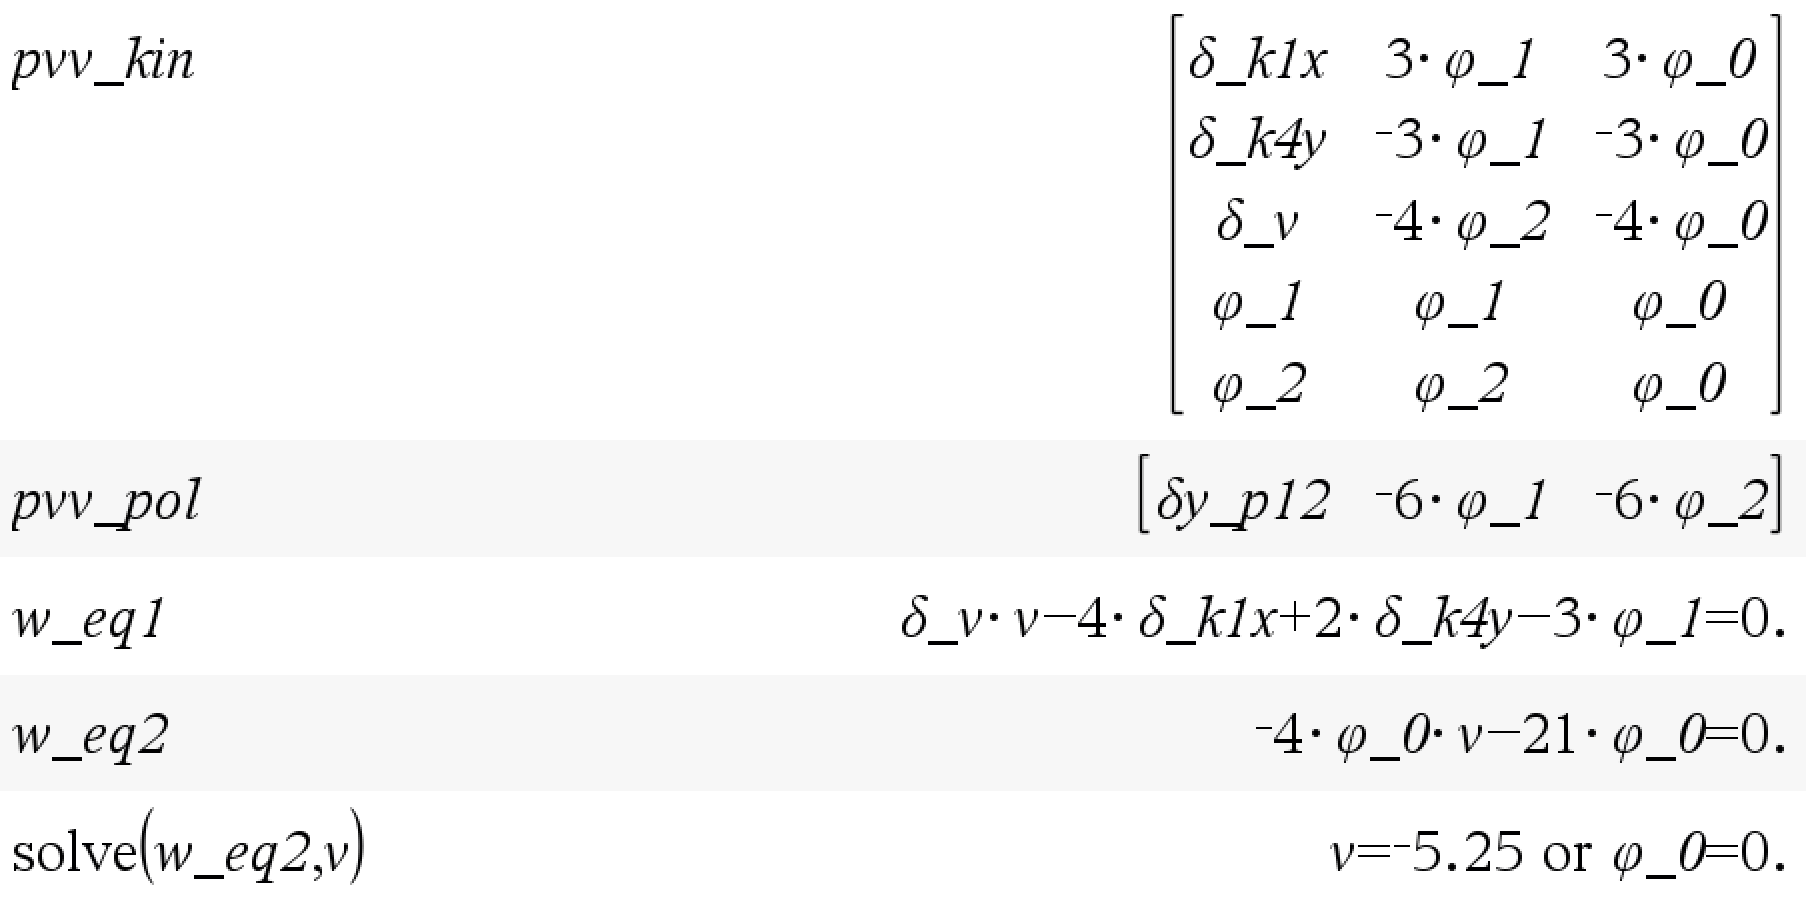
\includegraphics[width=\linewidth]{./fig/TM1/WiSe2122nr3_7.png}
        \caption{Rechnung für $B_V$}
    \end{subfigure}
    \caption{WiSe~21/22, Nr.~3: Ergebnis}
    \label{fig:TM1WiSe2122Nr3_4}
\end{figure}

\subsection{Schnittkräfte Bögen (Nr.~5)}

Mit dem Programm lassen sich die Funktionen für Schnittkraftverläufe von normalen Stäben als auch von Bögen 
ausgeben. Bei bögen ist die Laufvraibale nur nicht mehr die Länge entlang des Stabes sondern der Winkel.
also für diese Aufgabe zweilmal $\varphi \in [0,\frac{\pi}{4}]$ bzw. $\varphi \in [0,90\text{°}]$. Hier ist die Winkel-Einstellung
des Taschenrechenrs wichtig.\\
Hier gilt aber auch wieder, dass das Programm das nicht wirklich so ausrechnet wie man das von Hand machen würde, sondern
es sucht eine schöne Darstellung der Anfangswerte und kombiniert diese dann zur Funktion.

\begin{figure}[htbp]
    \centering
    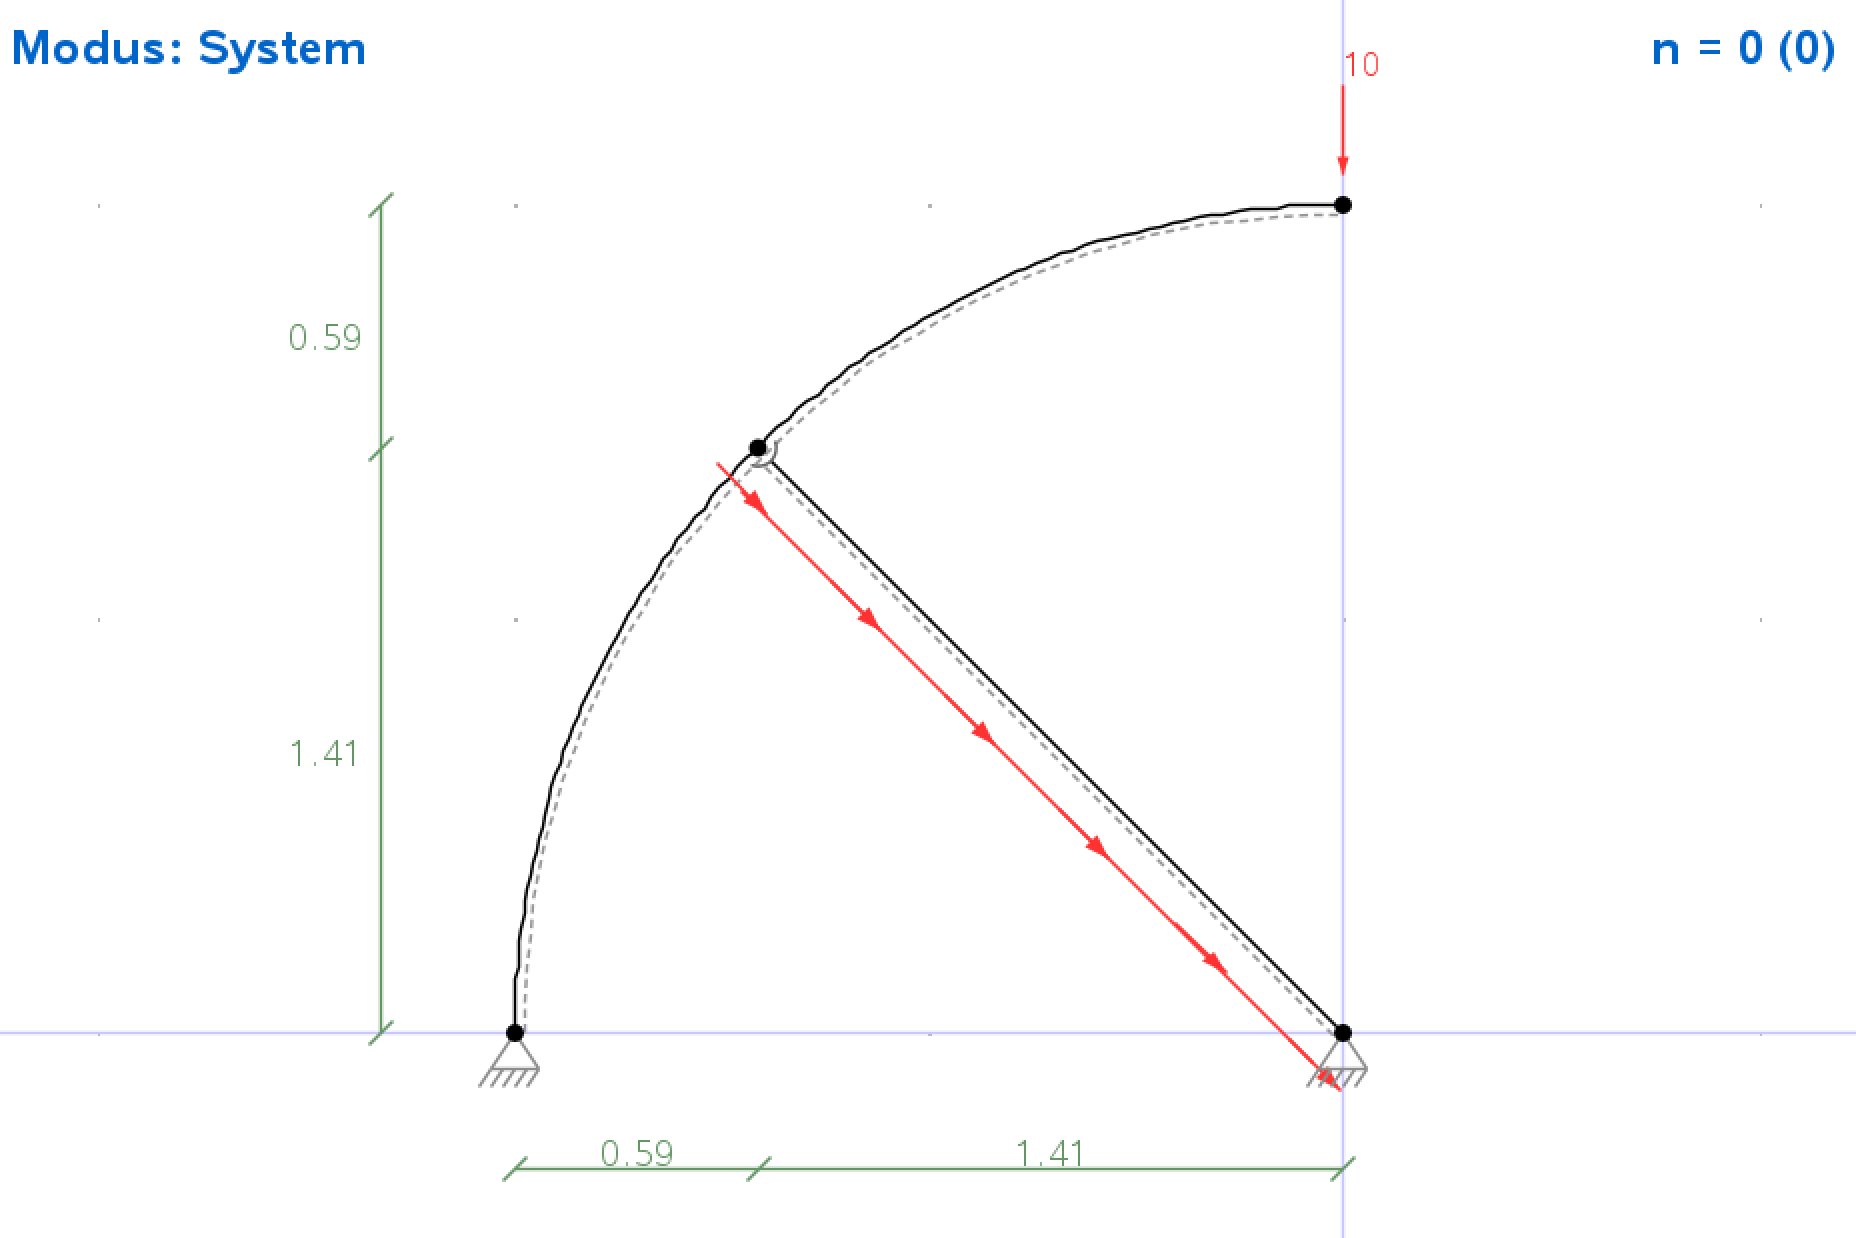
\includegraphics[width=0.5\linewidth]{./fig/TM1/WiSe2122nr5_1.png}
    \caption{TM1 WiSe~21/22, Nr.~5 im Programm}
    \label{fig:TM1WiSe2122Nr5_1}
\end{figure}


\subsection{Fachwerk (Nr.6)}

Vom Prinzip werden Fachwerke genau gleich eingegeben wie normale Systeme, nur das hier die orientierung der gestrichelten Faser
keine Rolle spielt. Es ist jedoch sinnvoll den Fachwerk Modus anzumachen, dann wird die statische Bestimmtheit beim hovern über $n=$ 
auch die Formel für Fachwerke verwendet und alle Knoten werden zu vollgelenken gemacht, auch wenn der Modus erst nach dem 
zeichnen des Systems angemacht wird.  


\begin{figure}[htbp]
    \centering
    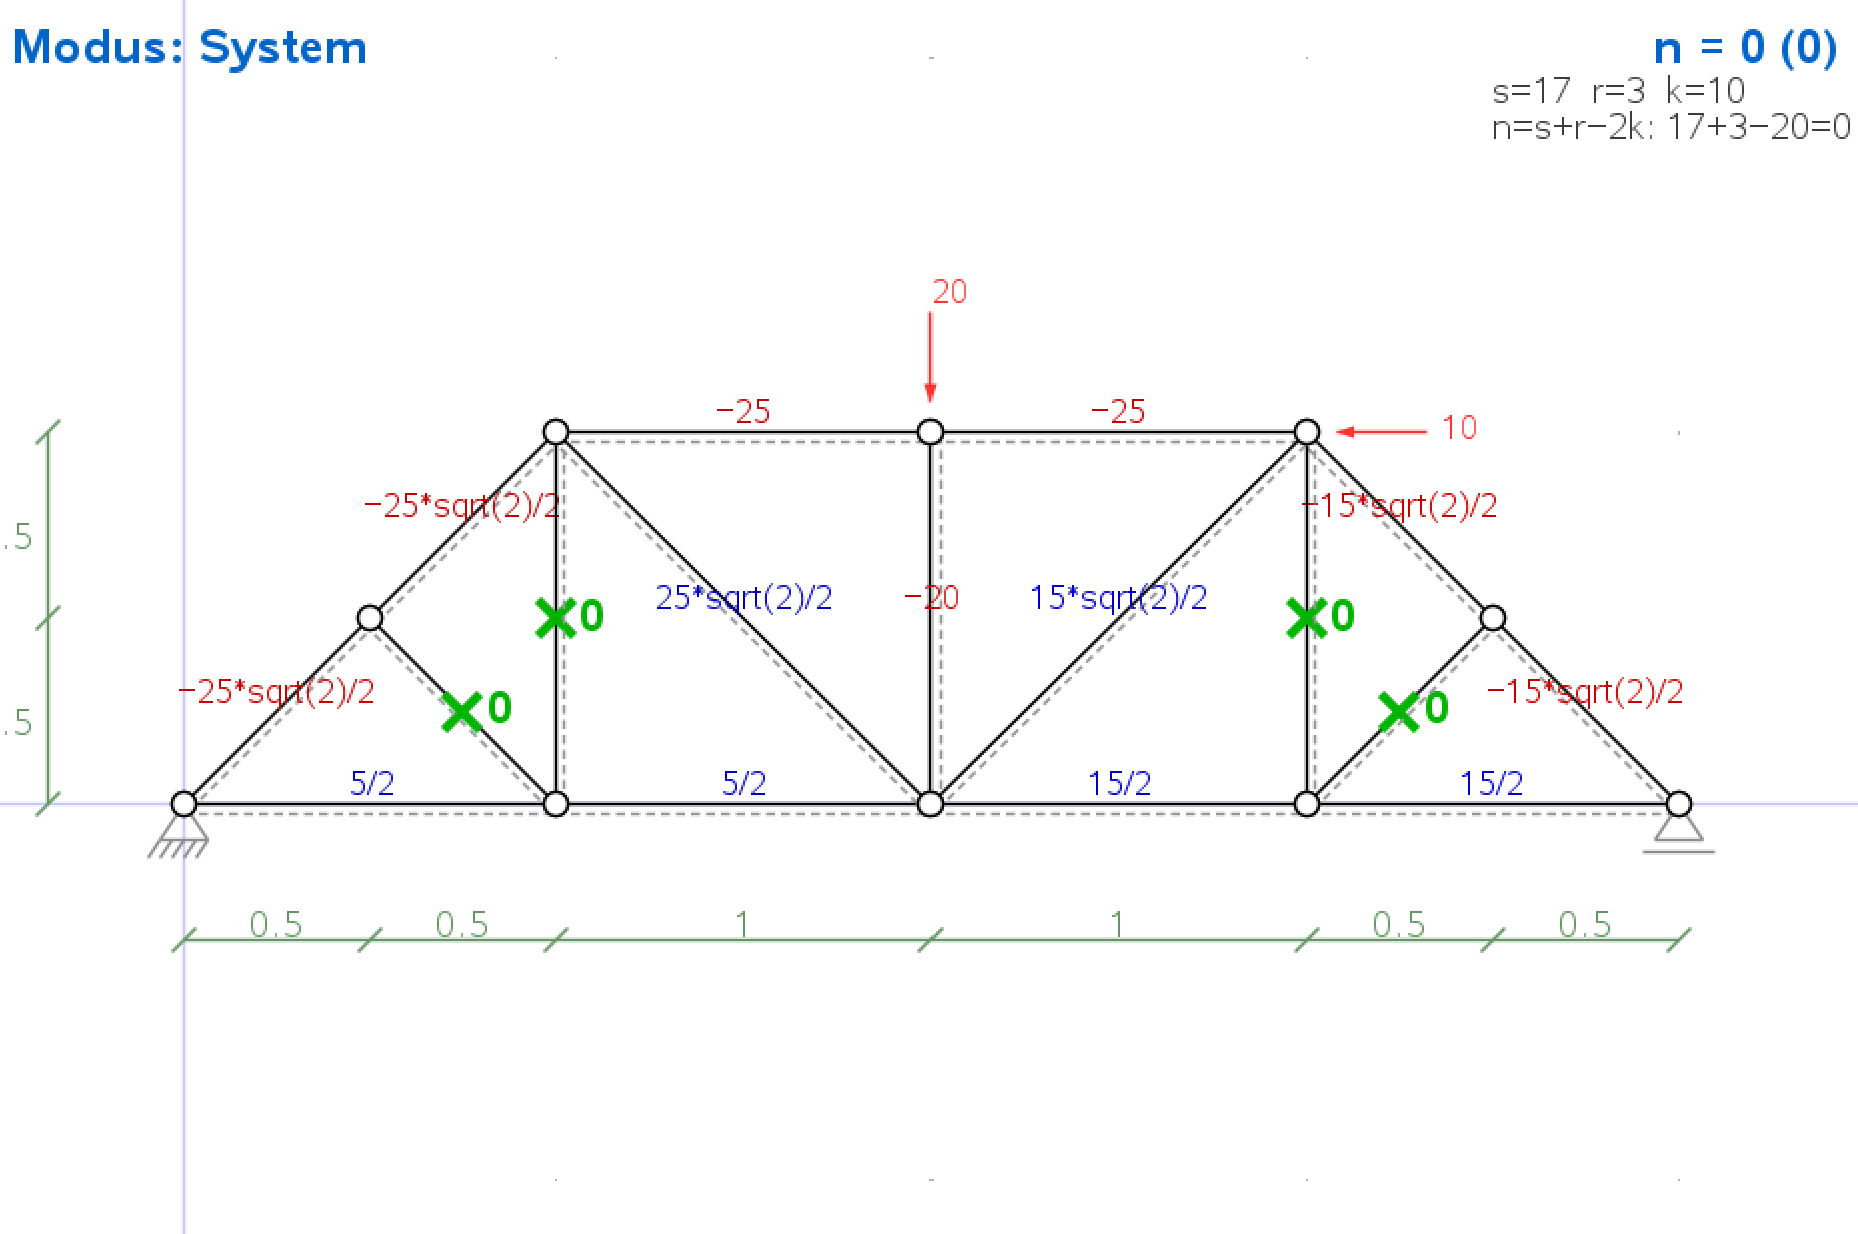
\includegraphics[width=0.5\linewidth]{./fig/TM1/WiSe2122nr6_1.png}
    \caption{TM1 WiSe~21/22, Nr.~6 im Programm}
    \label{fig:TM1WiSe2122Nr6_1}
\end{figure}

Die Stabe in Abb.~\ref{fig:TM1WiSe2122Nr6_1} die ein grünes Kreuz haben sind die ohne Rechnung erkennbaren Nullstäbe
Falls nach der Berechnung stäbkkräfte mit einer grünen Null beschriftet werdsen, aber dort kein Kreuz ist, ist das zwar ein 
Nullstab der aber nicht direkt aus den Regeln erkennbar ist. Für Afgaben bei denen nach Nullstäben gefragt wird, also nur 
die durchgekreuzten Stäbe angeben

\begin{figure}[htbp]
    \centering
    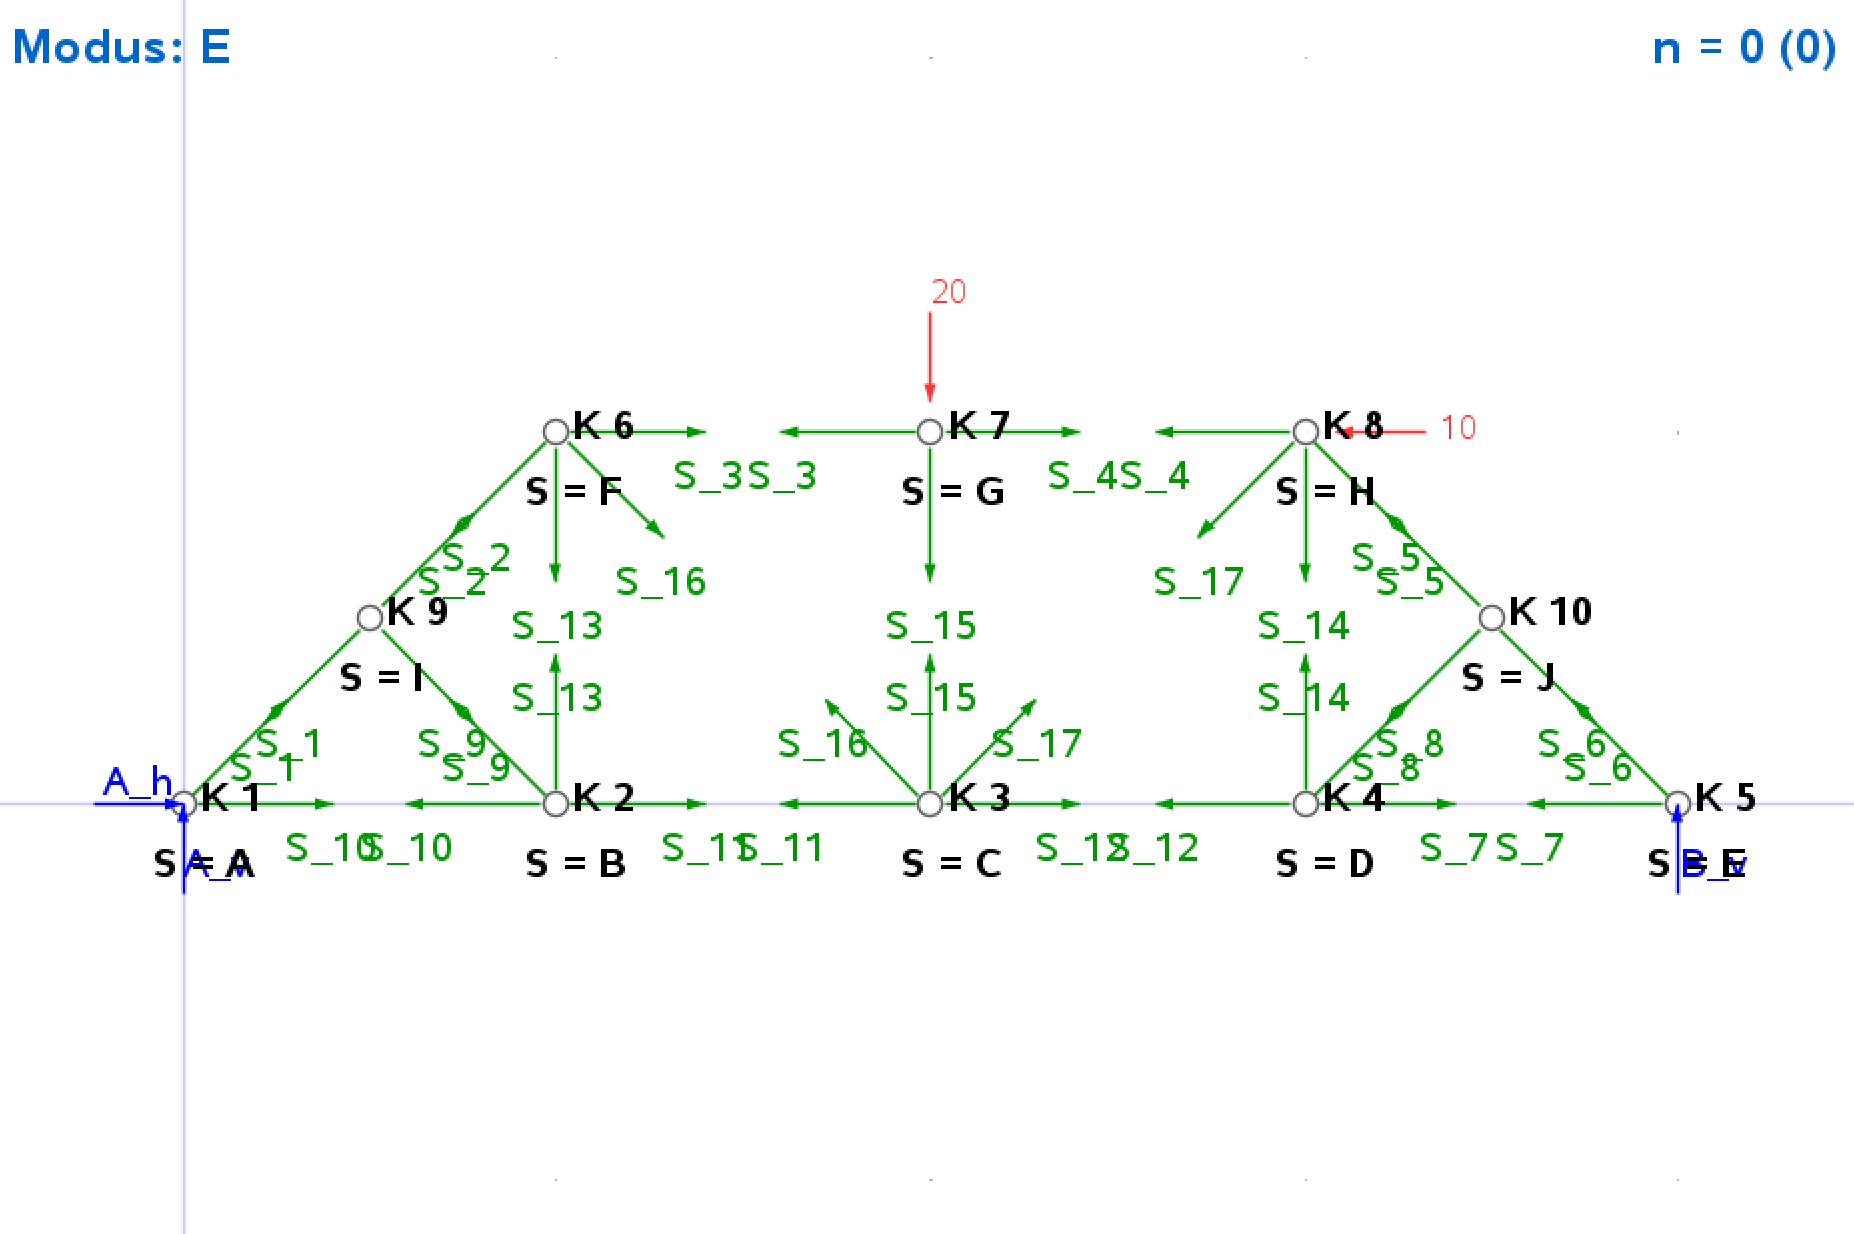
\includegraphics[width=0.5\linewidth]{./fig/TM1/WiSe2122nr6_2.png}
    \caption{TM1 WiSe~21/22 Freischnitt}
    \label{fig:TM1WiSe2122Nr6_2}
\end{figure}

Für die Verwendung der beiden Seiten des E-Modus muss darauf geachtet werden, dass entweder die Stäbe in der
gleichen Reihenfolge wie in der Aufgabe gezeichnet werden oder die Bennenung hinterher angepasst wird. Macht ihr das nicht
ist z.B. Stab 13 aus eurer Rechnung nicht Stab 13 aus der Aufgabe\\
Gleiches gilt natürlich auch für die Verwendung des LGS-Exports. Hier wird (Falls der Fachwerk Modus an ist) 
das Knotenschnittverfahren verwendet. Die Benennung im LGS ist die gleiche wie auf der zweiten Seite des E-Modus.





\section{TM2}

\subsection{Biegelinie (TM2 WiSe~21/22, Nr.~7)} \label{ex:Biegelinienaufgabe}

In dieser Aufgabe ist ein \emph{interessantes} KOS vorgegeben: Soll es ein Rechtssystem sein,
zeigt die $y$-Achse hier in die Zeichenebene hinein und nicht, wie sonst üblich, aus ihr heraus.

Rechnet ihr von Hand über die DGL $EI\,w'''' = q$ mit allen Rand- und Übergangsbedingungen (so
geht man bei statisch unbestimmten Systemen meist vor, und so rechnet auch \code{wneu}), gibt es
hier nichts weiter zu beachten. Bei einem statisch bestimmten System lohnt es sich dagegen, zuerst
die Momentenlinie zu berechnen und dann $EI\,w'' = -M$ zu integrieren. Dafür braucht ihr die
gestrichelte Faser. Die Regel aus Abschnitt~\ref{sec:Eingabe_Stäbe}, dass sie immer auf der Seite
liegt, in die die $z$- bzw.\ $w$-Achse zeigt, gilt auch hier. Alternativ könnt ihr euch überlegen,
auf welcher Seite ein positives Schnittmoment $M_y$ (Drehsinn nach der Rechte-Hand-Regel um die
$y$-Achse) Zug erzeugt, dort liegt die gestrichelte Faser. Das finde ich aber umständlicher.

Im Programm müsst ihr solche Systeme etwas anders eingeben, denn dort zeigt die $y$-Achse immer
aus der Zeichenebene heraus. Zeichnet ihr das System genau wie in der Aufgabe und setzt die
gestrichelte Faser nach der Regel oben, läuft die $x$-Koordinate im Programm in die andere Richtung
als in der Aufgabe. Um das zu umgehen, zeichnet ihr Systeme, bei denen die $y$-Achse in die
Zeichenebene hineinzeigt, spiegelverkehrt (Abb.~\ref{fig:Biegelinienaufgabe}). Ich habe die
Aufgabe im symbolischen Modus gerechnet, deshalb stehen in den Ergebnissen $q$ und $l$.

\begin{figure}[htbp]
    \centering
    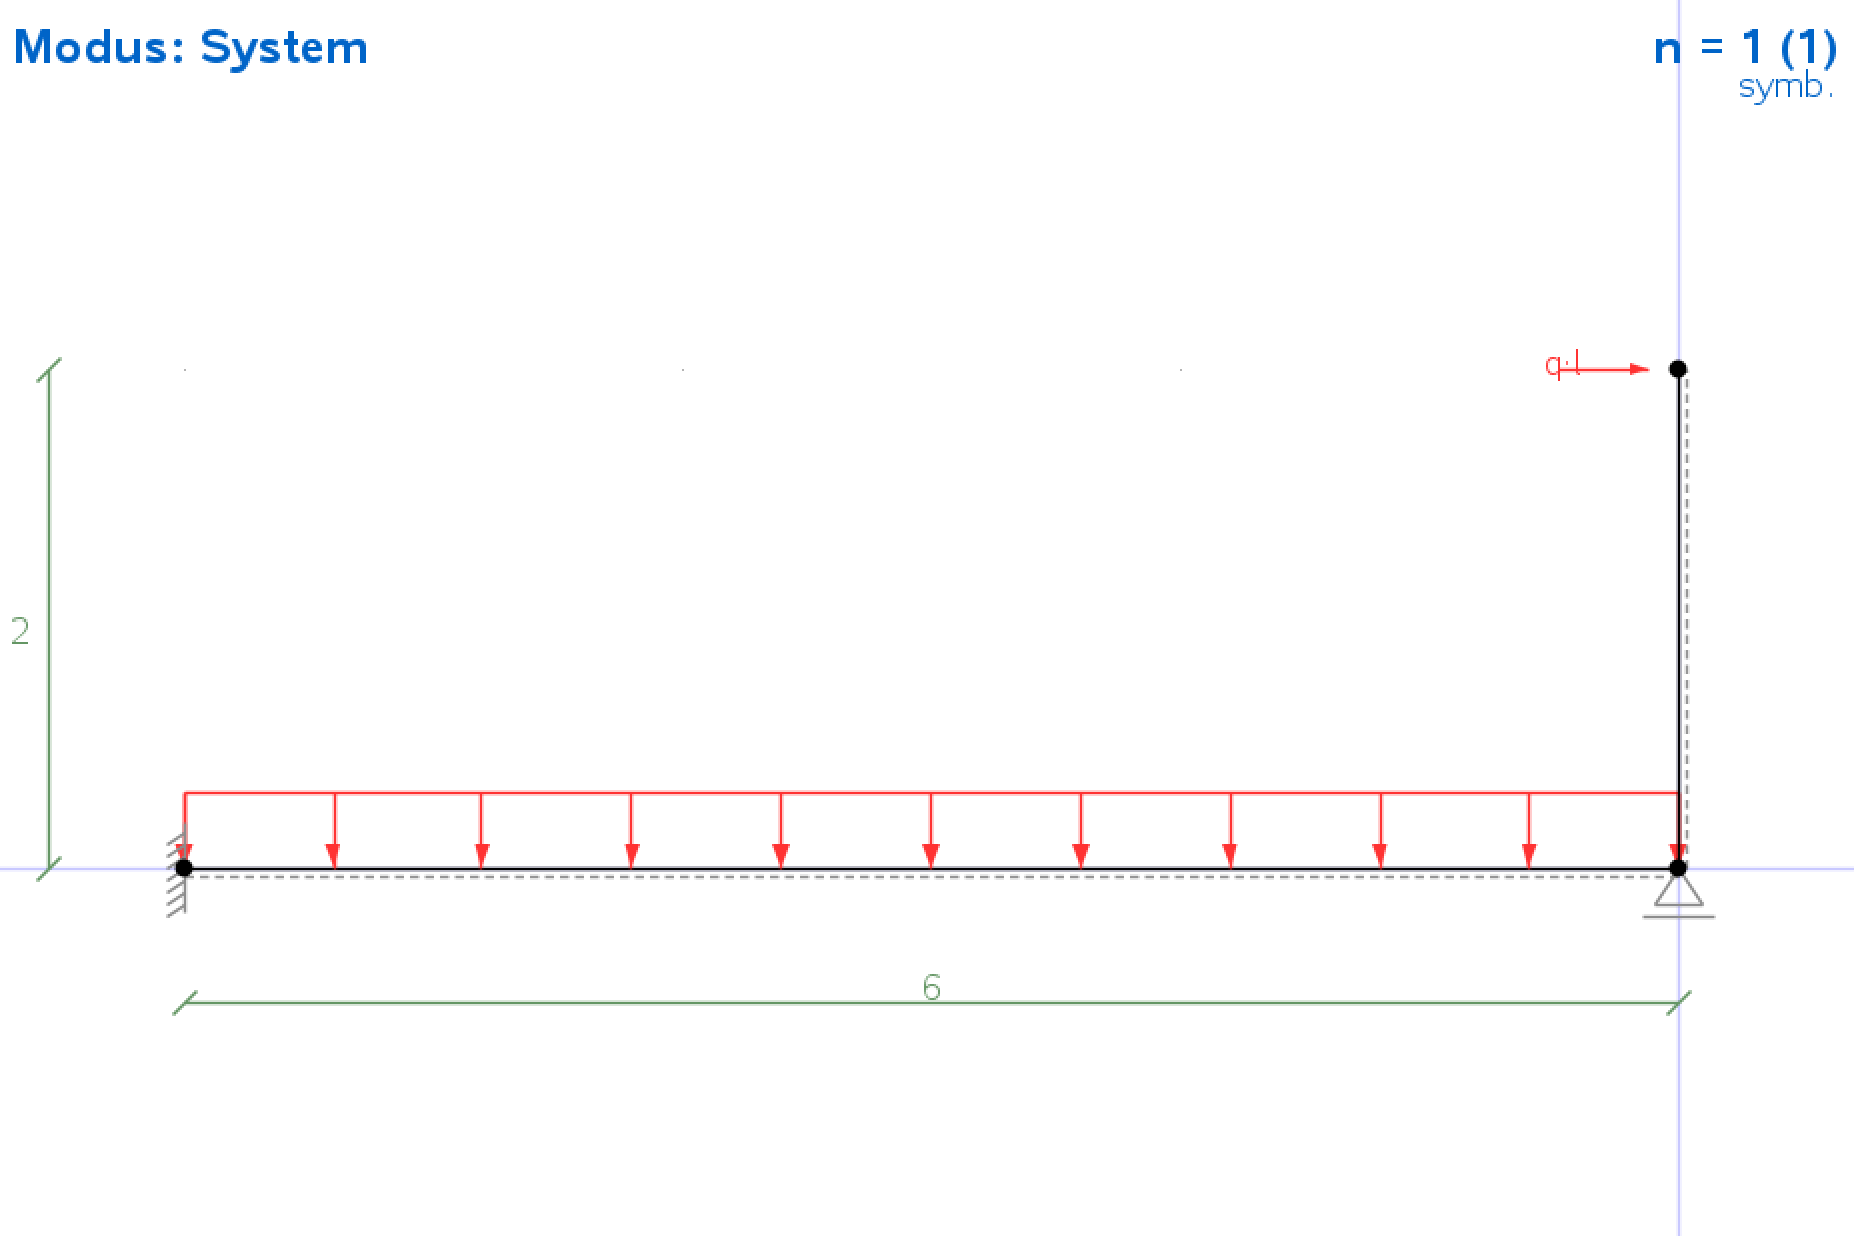
\includegraphics[width=0.5\linewidth]{./fig/TM2/WiSe2122nr7_1.png}
    \caption{TM2 WiSe~21/22, Nr.~7 im Programm, spiegelverkehrt gezeichnet}
    \label{fig:Biegelinienaufgabe}
\end{figure}

Das liefert die Ergebnisse in Abb.~\ref{fig:BiegelinienaufgabeBiegelinie}. Hier geben beide
Methoden dasselbe Ergebnis. Das sollte natürlich so sein, ist aber nicht immer so: Manchmal weicht
die WGV/FEM-Lösung \code{v\_EI\_stab1(x)} (im Rechner klein geschrieben) minimal von der exakten
Lösung \code{wneu1(x)} ab. Weil das Programm die Brüche aus den Zahlen der FEM-Lösung
\emph{errät} (Abschnitt~\ref{sec:mathe-symbolisch}), kann daraus eine ganz anders aussehende
Biegelinie werden. Die Methode über die WGV/FEM-Lösung gibt es trotzdem, vor allem weil ich sie
zuerst programmiert habe (daher wohl auch der Name \code{wneu} der anderen Funktion), und weil sie
bei sehr großen Systemen deutlich schneller sein kann.

\begin{figure}[htbp]
    \centering
    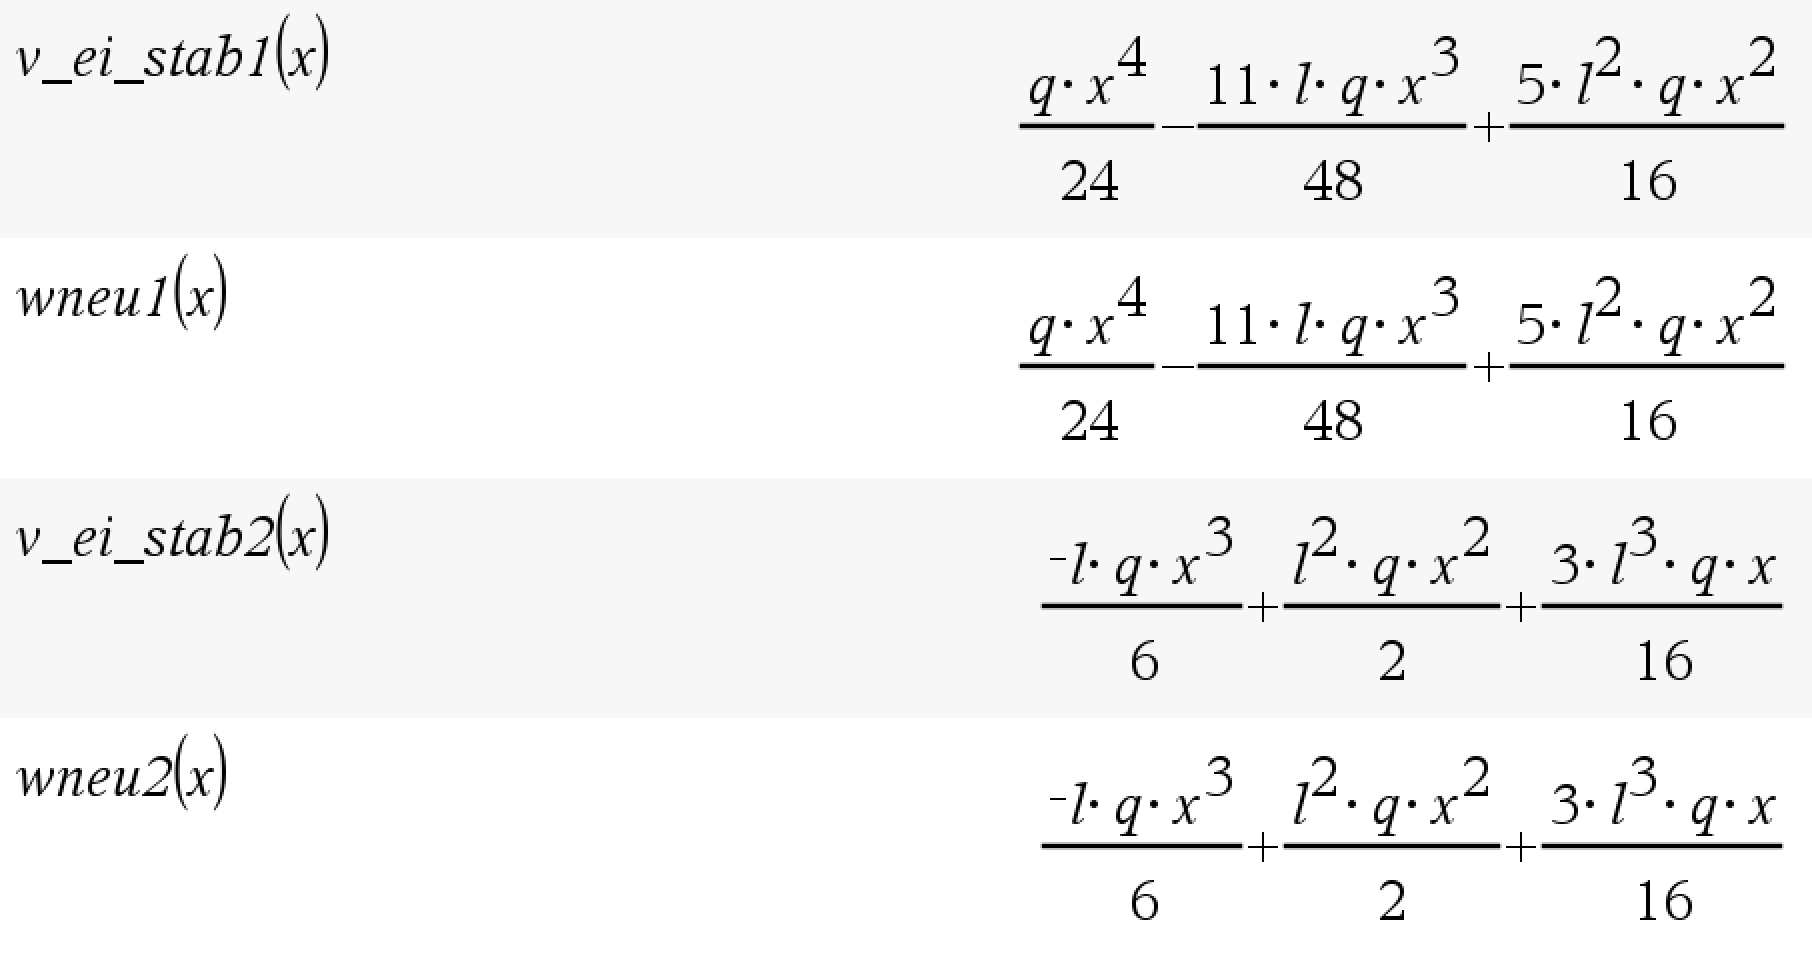
\includegraphics[width=0.5\linewidth]{./fig/TM2/WiSe2122nr7_2.png}
    \caption{TM2 WiSe~21/22, Nr.~7: \code{v\_EI\_stab} und \code{wneu} im Vergleich}
    \label{fig:BiegelinienaufgabeBiegelinie}
\end{figure}

Weil die Stäbe dehnsteif sind, kann das Programm hier sogar die Randbedingungen für Biegelinie und
Längslinie getrennt angeben (Abb.~\ref{fig:BiegelinienaufgabeRandbed}): Die Bedingungen im oberen
Block reichen für die Biegelinie allein, die im unteren kommen nur für die Längslinie dazu. Das geht
nicht immer. Sind die Stäbe dehnbar, hängt die Biegelinie über die Rahmenecken auch von den
Längsverformungen ab, und das Programm gibt alle Bedingungen zusammen aus
(Abschnitt~\ref{sec:randlgs}).

\begin{figure}[htbp]
    \centering
    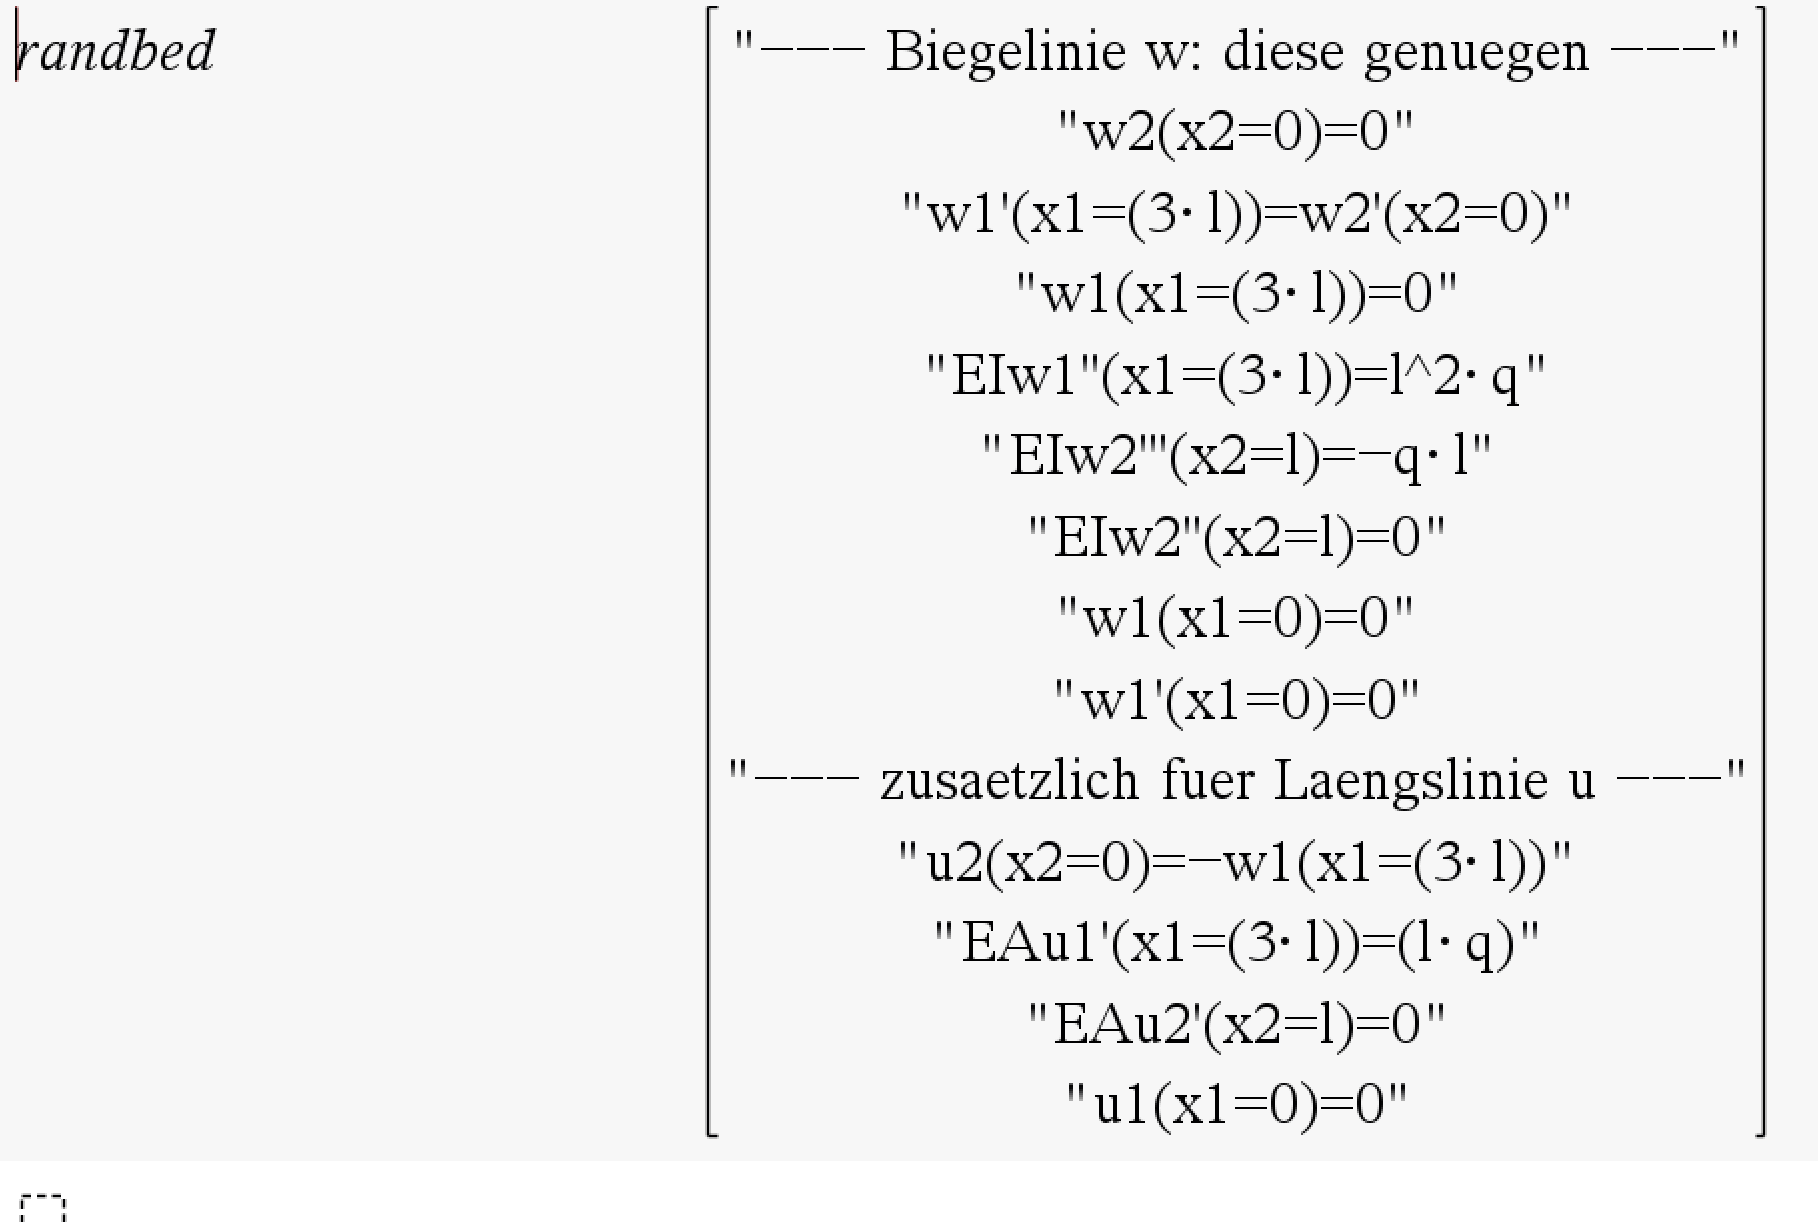
\includegraphics[width=0.5\linewidth]{./fig/TM2/WiSe2122nr7_3.png}
    \caption{Randbedingungen \code{randbed} für TM2 WiSe~21/22, Nr.~7}
    \label{fig:BiegelinienaufgabeRandbed}
\end{figure}



\subsection{Verschiebungsaufgaben (TM2 WiSe~20/21 Nr.~4)} \label{ex:Temperaturaufgabe}

Aufgaben wie diese lassen sich mit der richtigen Eingabe auch direkt im Programm lösen. Wie diese Aufagbe im
Programm aussieht ist in Abb.~\ref{fig:verschiebungSystem} dargestellt. Hierbei muss natürlich auf die Einheiten geachtet werden.
In der Aufgabe sind die relevanten Dehnsteifigkeiten nicht direkt gegeben, genauso wie manche Angaben nicht in der
für das Programm geforderten Einheit sind.\\
Für Kräfte immer kN, genauso wie für die Dehnsteifigkeit $EA$ und die Biegesteifigkeit $EI$ in kNm.  

\begin{figure}[htbp]
    \centering
    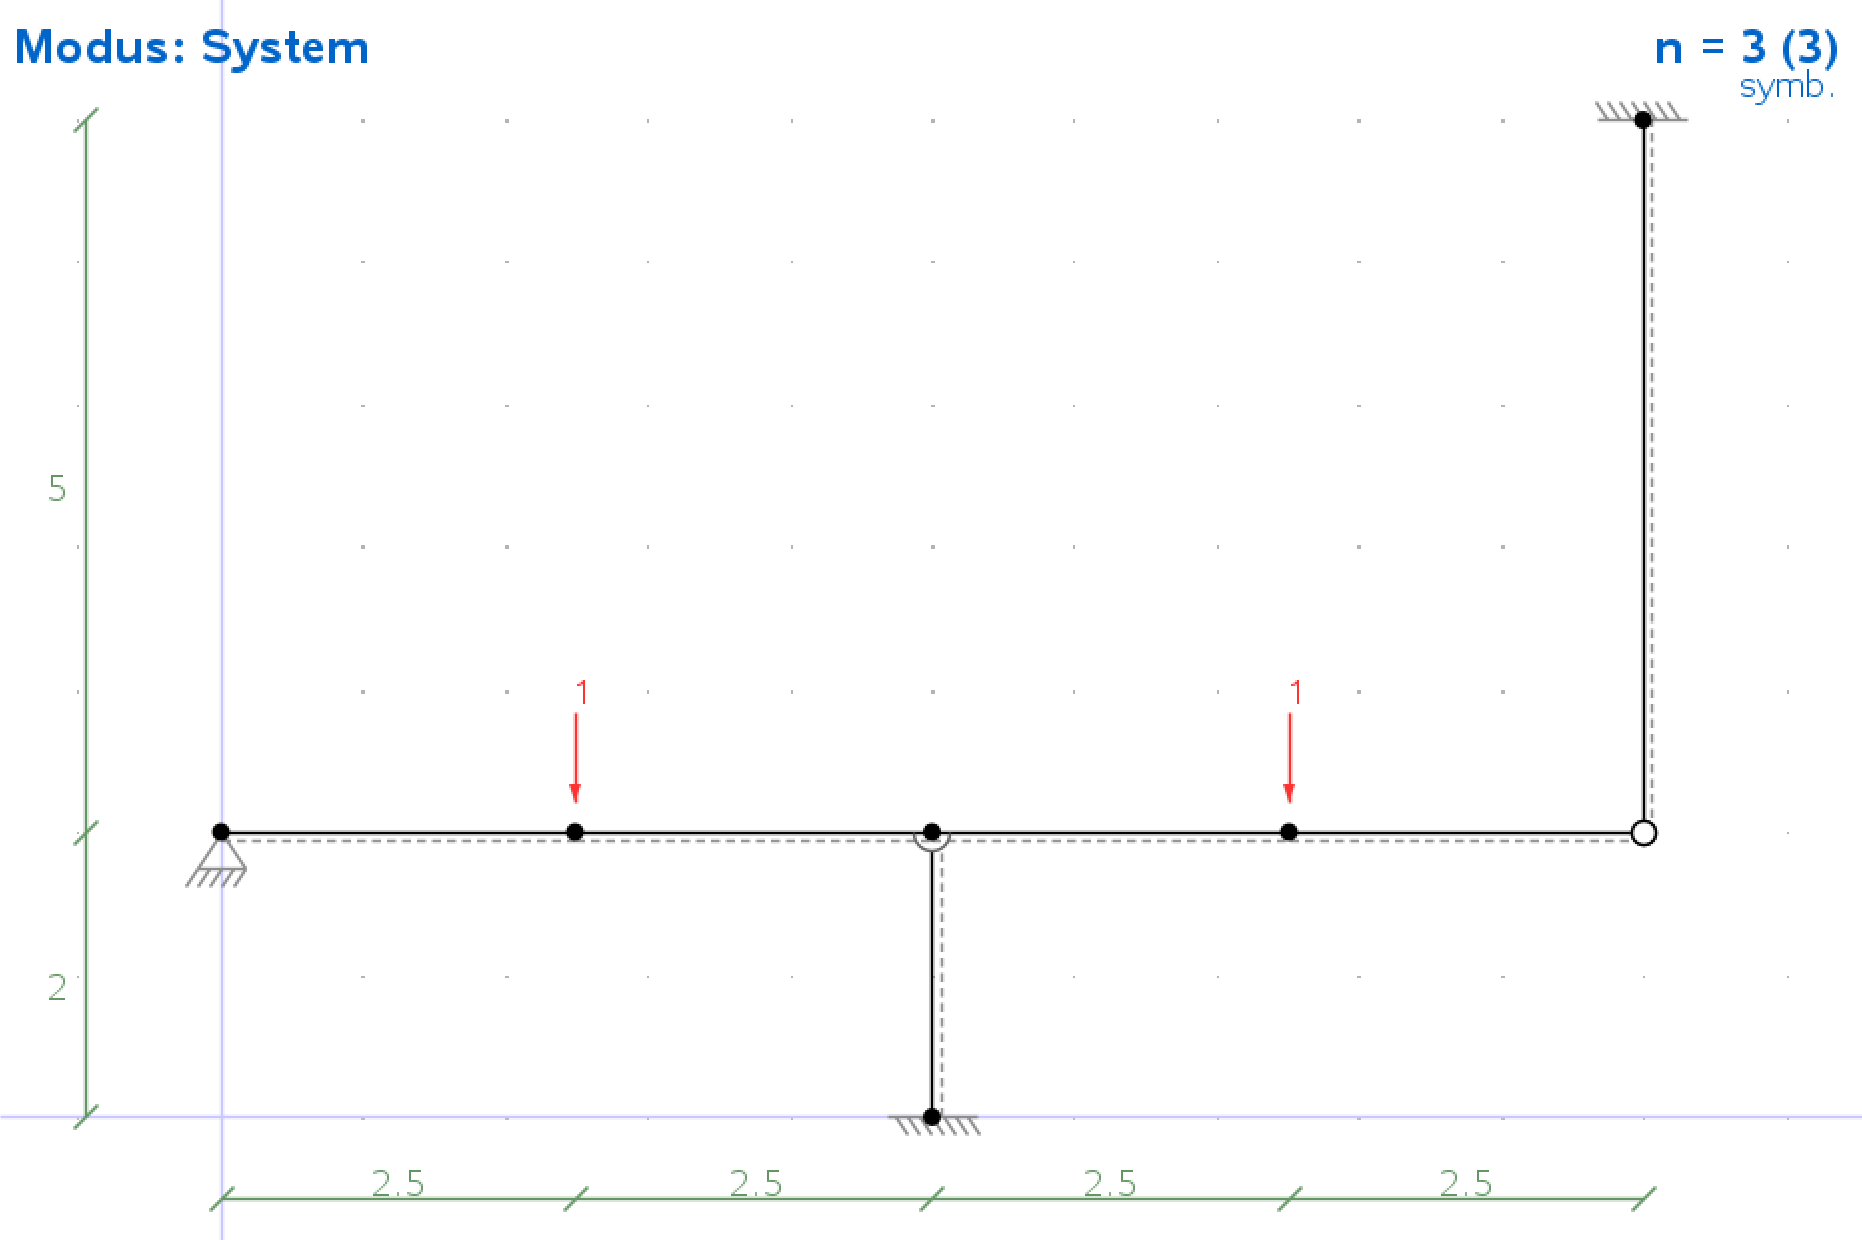
\includegraphics[width=0.5\linewidth]{./fig/TM2/WiSe2021nr4_1.png}
    \caption{TM2 WiSe~20/21, Nr.~4a im Programm}
    \label{fig:verschiebungSystem}
\end{figure}

In den \emph{neuen} Exportfunktionen wird die Temperatur auch symbolisch miteinberechnet.
Um also ann die Verschiebung des rechten unteren Knoten zu kommen lässt sich das entweder über die obere
Knotenexportfunktion machen, über die Biegelinie des rechten horizontalen Stabes oder über die Längsverschiebungsfunktion
des rechten vertikalen Stabes. Über den CAS Befehl \code{solve()} lässt sich die Temperatur direkt ausrechnen 
(vgl. Abb.~\ref{fig:verschiebungErgebniss}). Ich habe hier die Tempertur $dt$ genant (nur $T$ ist wie bereits erwähnt nicht erlaubt),
die Variable nach der aufgelöst werden soll muss der \code{solve()} Funktion als zweites Argument mit gegeben werden.

\begin{figure}[htbp]
    \centering
    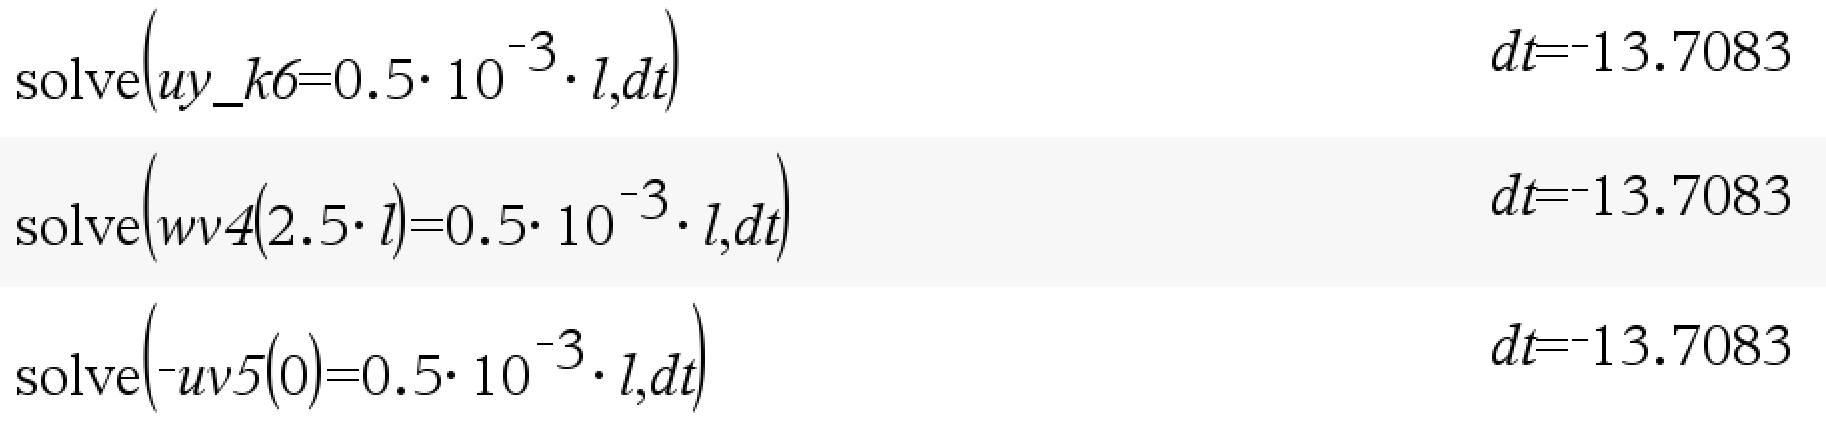
\includegraphics[width=0.5\linewidth]{./fig/TM2/WiSe2021nr4_2.png}
    \caption{Lösung von TM2 WiSe~20/21, Nr.~4a}
    \label{fig:verschiebungErgebniss}
\end{figure}

Der Zweite Teil der Aufgabe lässt sich auch im Programm lösen (Abb.~\ref{fig:VerschiebungTemp}), jedoch gibt es auch hier
ein paar Feinheiten. Ein deratiges System zu speichern kann sich lohnen. Auch hier gelten natürlich die gleichen Hinweise zu den Einheiten.

\begin{figure}[htbp]
    \centering
    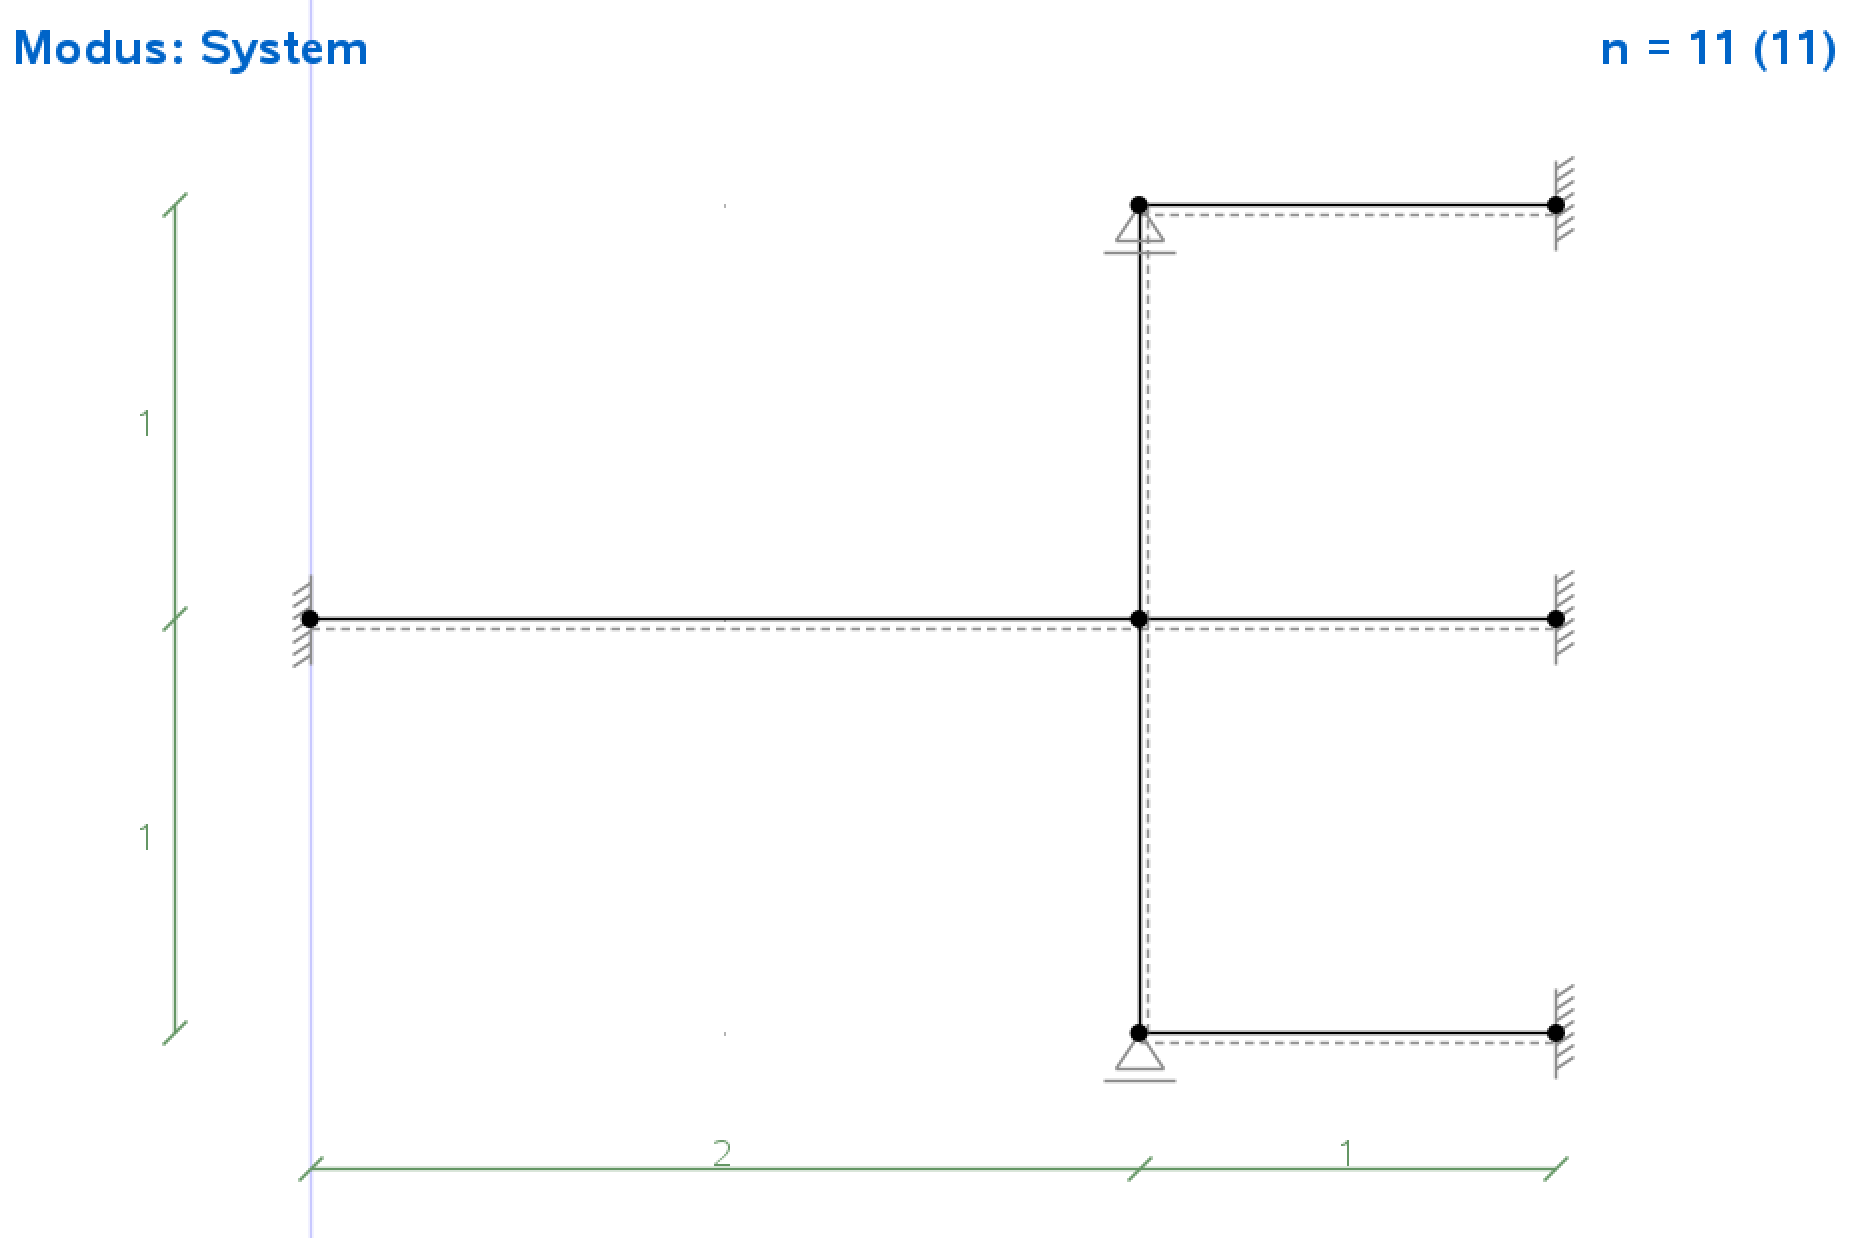
\includegraphics[width=0.5\linewidth]{./fig/TM2/WiSe2021nr4_3.png}
    \caption{TM2 WiSe~20/21, Nr.~4b im Programm}
    \label{fig:VerschiebungTemp}
\end{figure}

Da das Programm nur schnittgrößen direkt berechnet müssen diese noch in Spannungen umgerechnet werden, dafür gibt es in diesem Fall
zwei Möglichkeiten (vgl. Abb.\ref{fig:TM2WiSe2021Nr4b}). Entweder man rechnet die Spannunge direkt über die Schnittkraftverläufe aus,
oder über die Ableitung der Verschiebungsfunktion. Für die zweite Methode muss jedoch darauf geachtet werden den Temperatur Anteil
korrekt zu verrechnen.\\
Erstere Methode ist für Aufgaben mit Zahlenwerten auf jeden Fall die Einfachere, für Aufgaben mit symbolischen Temperatur Werten muss jedoch
die zweite Methode gewählt werden, da die Schnittkraftverläufe diese nicht auf die gewünschte Art berücksichtigen.

\begin{figure}[htbp]
    \centering
    \begin{subfigure}[t]{0.48\textwidth}
        \centering
        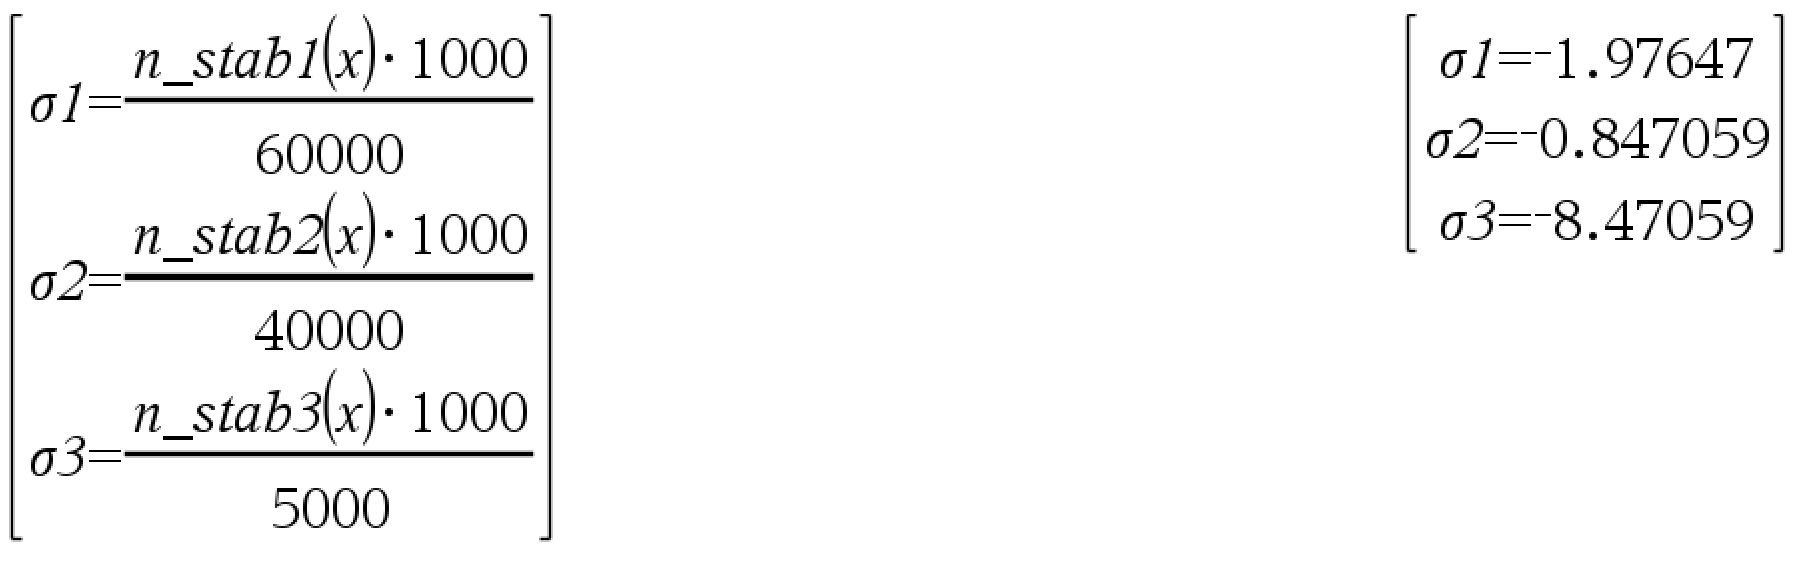
\includegraphics[width=\linewidth]{./fig/TM2/WiSe2021nr4_4.png}
        \caption{Über Schnittgrößen}
    \end{subfigure}
    \hfill
    \begin{subfigure}[t]{0.48\textwidth}
        \centering
        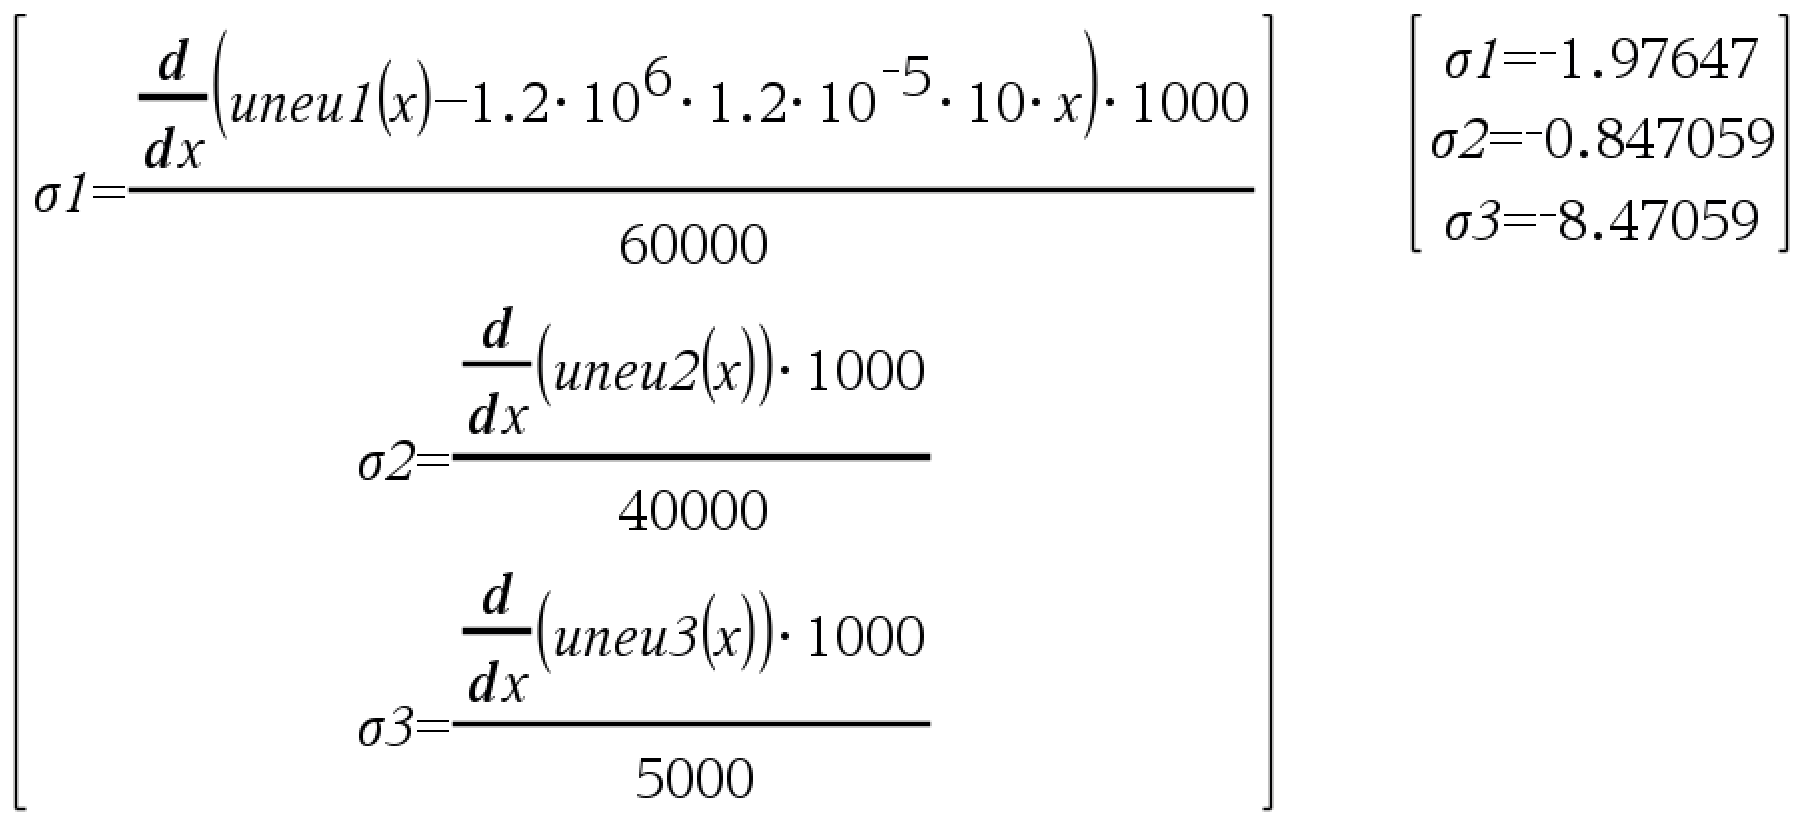
\includegraphics[width=\linewidth]{./fig/TM2/WiSe2021nr4_5.png}
        \caption{Über Verschiebungsfunktion}
    \end{subfigure}
    \caption{Lösung von TM2 WiSe~20/21, Nr.~4b}
    \label{fig:TM2WiSe2021Nr4b}
\end{figure}

Ich will hier anmerken das bei dieser Aufgabenart häufig Hinweise und Warnungen angezeigt werden. Wie z.B. hier auch bei Teilaufgabe a) eine Warnung
zur symbolischen Temperatur. Diese Warnungen sind zwar so konzipiert, dass sie nur angezeigt werden wenn das Programm bzw. ich denke
das etwas falsch eingegeben wurde, jedoch ist es schwer dabei zu vermeiden das auch bei richtiger Eingabe nie eine Warnung oder Hinweis kommt.
Aus diesem Grund empfehele ich, wenn nicht direkt ersichlich ist warum eine Warnung kommt die komplette Eingabe nochmal zu prüfen,
falls diese aber wirklicht korrekt ist sollten auch die Ergebnisse stimmen.


\subsection{Pendelstabannahme (TM2 WiSe 22/23 Nr.~4)} \label{ex:Pendelstabannahme}

\begin{figure}[htbp]
    \centering
    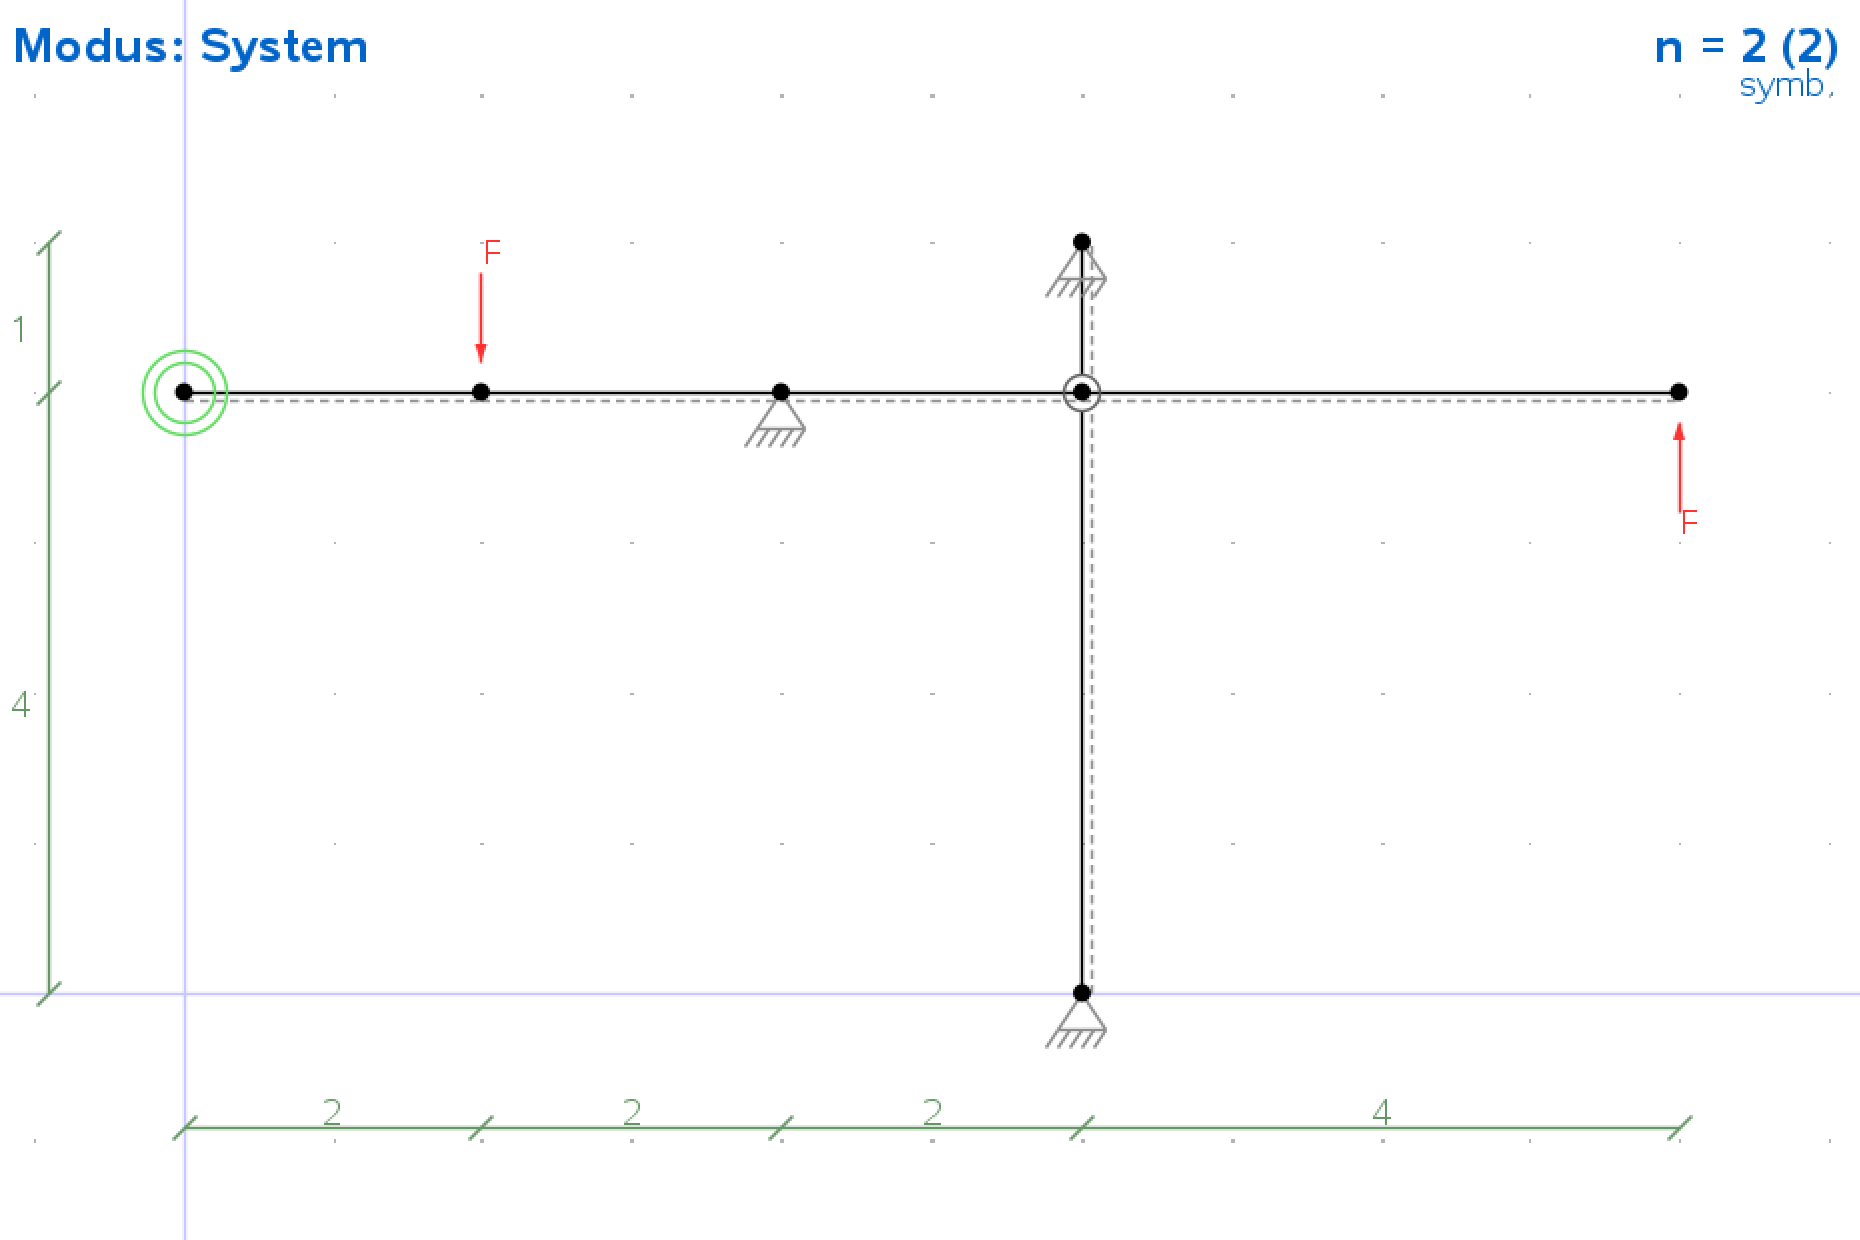
\includegraphics[width=0.7\linewidth]{./fig/TM2/WiSe2223nr4_1.png}
    \caption{TM2 WiSe~22/23, Nr.~4 im Programm}
    \label{fig:Pendelstabsnnahme}
\end{figure}

Wie die Überschrifft vielleicht bereits vermuten lässt muss bei dieser Aufgabe eine Annahme getroffen werden,
die der Zeichnung strenggenommen wiederspricht. Die beiden vertikalen stäbe sollten eigentlich mit einem Angelenk
an den starren Stab angeschlossen werden.\\
Bei einer Handrechnung wird diese Annahme quasi automatisch getroffen, das Programm macht sowas natürlich nicht automatisch.
Um diese Aufgabe mit dem Programm also korrekt zu rechnen müsseb bei den beiden vertikalen stäbe jeweils Angelenke eingebaut werden.
Falls man das nicht macht wirft das Programm eine Warnung bzw. einen Hinweis.

Bei dieser Aufgabe lassen sich die Ergebnisse entweder aus der Ansicht zur Normalkraft 
oder aus dem E-Modus holen (Abb.~\ref{fig:TM2WiSe2223Nr4}).

\begin{figure}[htbp]
    \centering
    \begin{subfigure}[t]{0.48\textwidth}
        \centering
        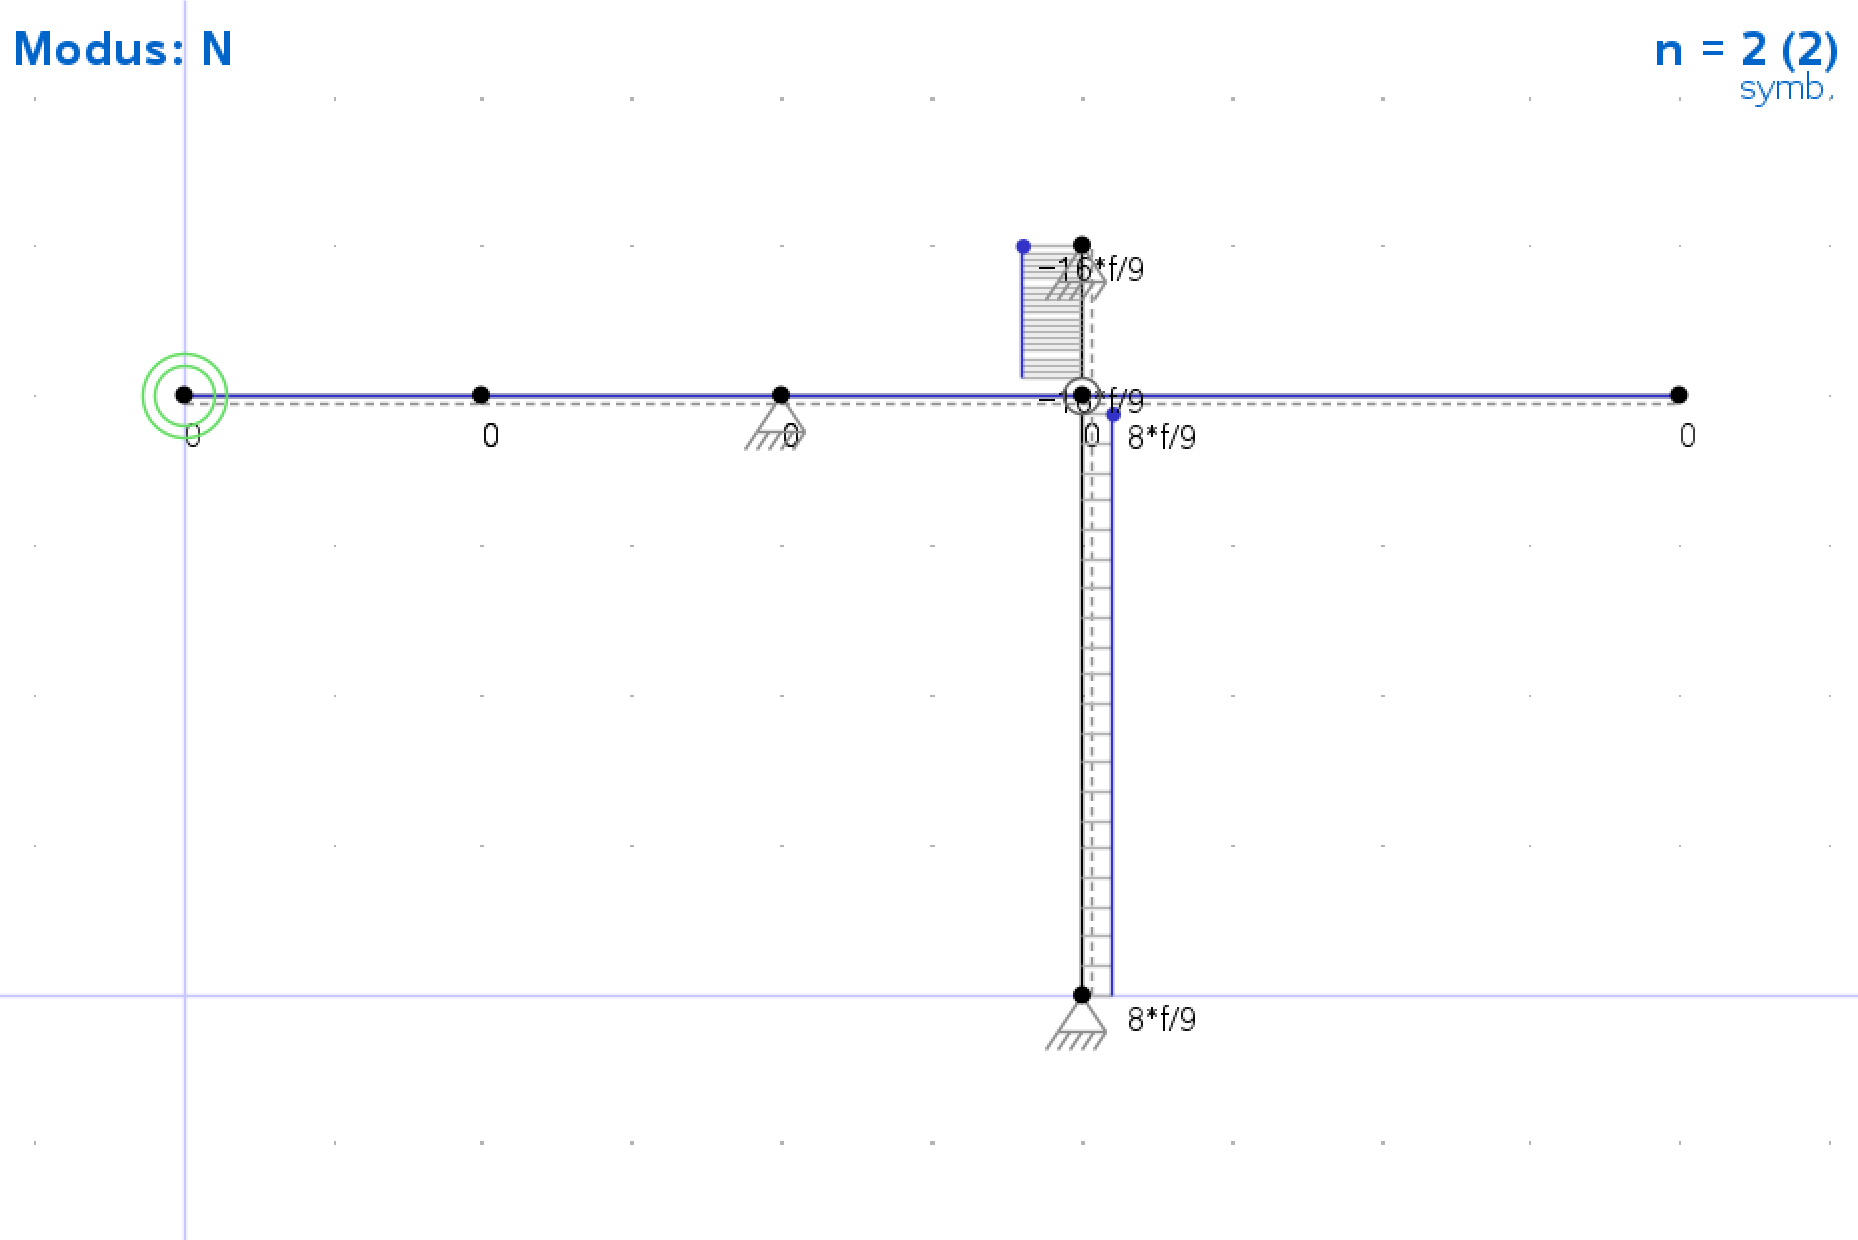
\includegraphics[width=\linewidth]{./fig/TM2/WiSe2223nr4_2.png}
        \caption{Normalkraft}
    \end{subfigure}
    \hfill
    \begin{subfigure}[t]{0.48\textwidth}
        \centering
        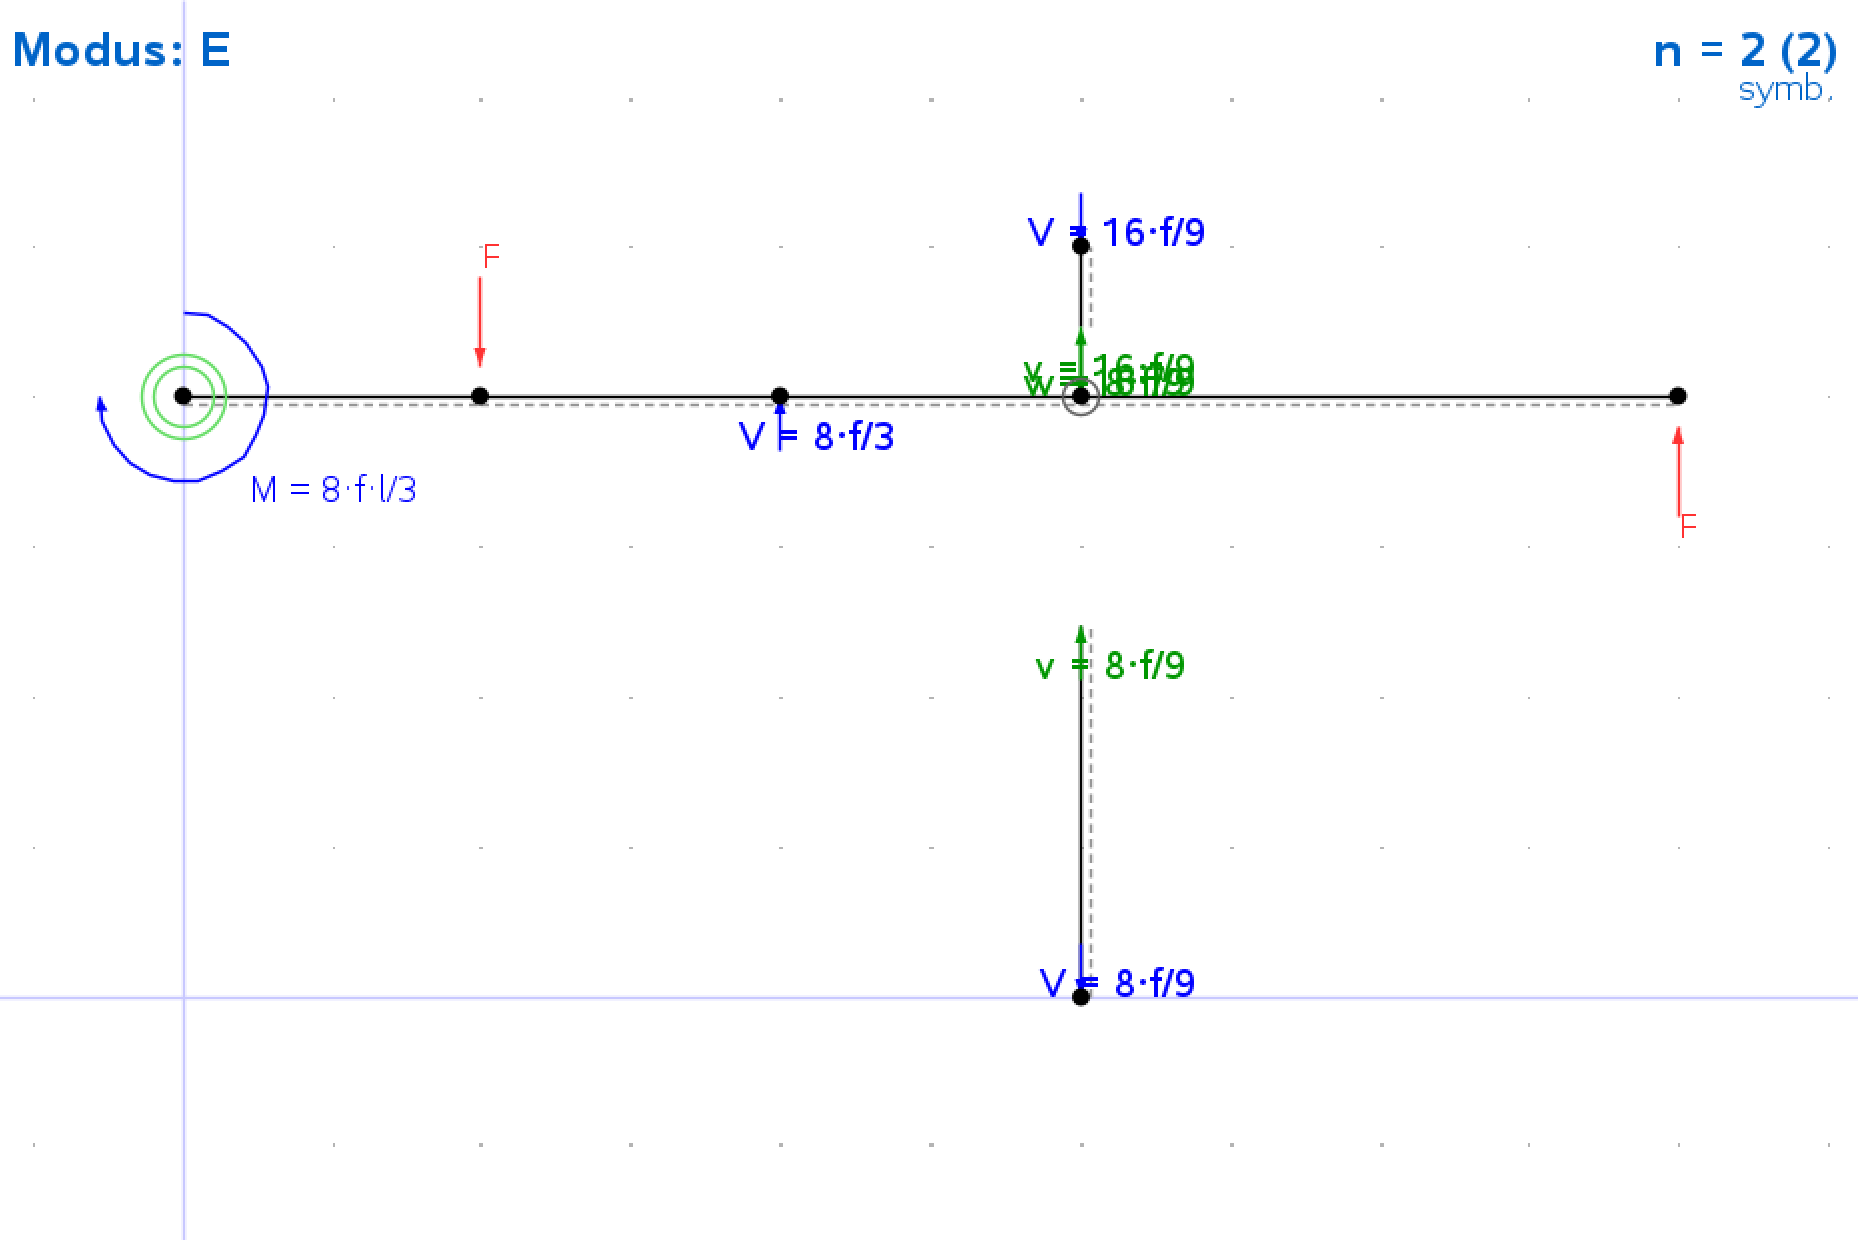
\includegraphics[width=\linewidth]{./fig/TM2/WiSe2223nr4_3.png}
        \caption{E-Modus}
    \end{subfigure}
    \caption{Lösung von TM2 WiSe~22/23, Nr.~4}
    \label{fig:TM2WiSe2223Nr4}
\end{figure}

\textbf{Wichtig} ist, dass das Programm, für symbolische Federn in den Verläufen in seltenen Fällen nicht die richtigen 
Werte ausgibt (Bei symbolischen Temperaturen sowieso nicht).
Zur Sicherheit würde ich deswegen die Schnittgrößen über die \emph{neuen} Verschiebungsfunktionen ermitteln. 
Das dauert zwar gerade für große Systeme länger, ist aber zuverlässiger weil dort wirklich alles symbolisch gerechnet wird 
und eben nicht gepfuscht wird.



\subsection{Schiefe Biegung (TM2 WiSe 25/26 Nr.~8)}

In dieser Aufgbabe sind die Dicken der dünnwandigen Elemente nicht gegeben, da diese abber sowohl für das
FTM als auch für die Lange des Schwerpunkts wichtig sind, müssen diese Werte manuell mit den Werten aus der 
Aufgabenstellung überschrieben werden. Das geht im Obermenue (Taste \taste{o}) auf Seite 3.\\
Für das Zeichnen so eines schiefen Querschnitts empfielt sich ein Rastermaß von z.B. $\frac{1}{\sqrt{2}}$.

\begin{figure}[htbp]
    \centering
    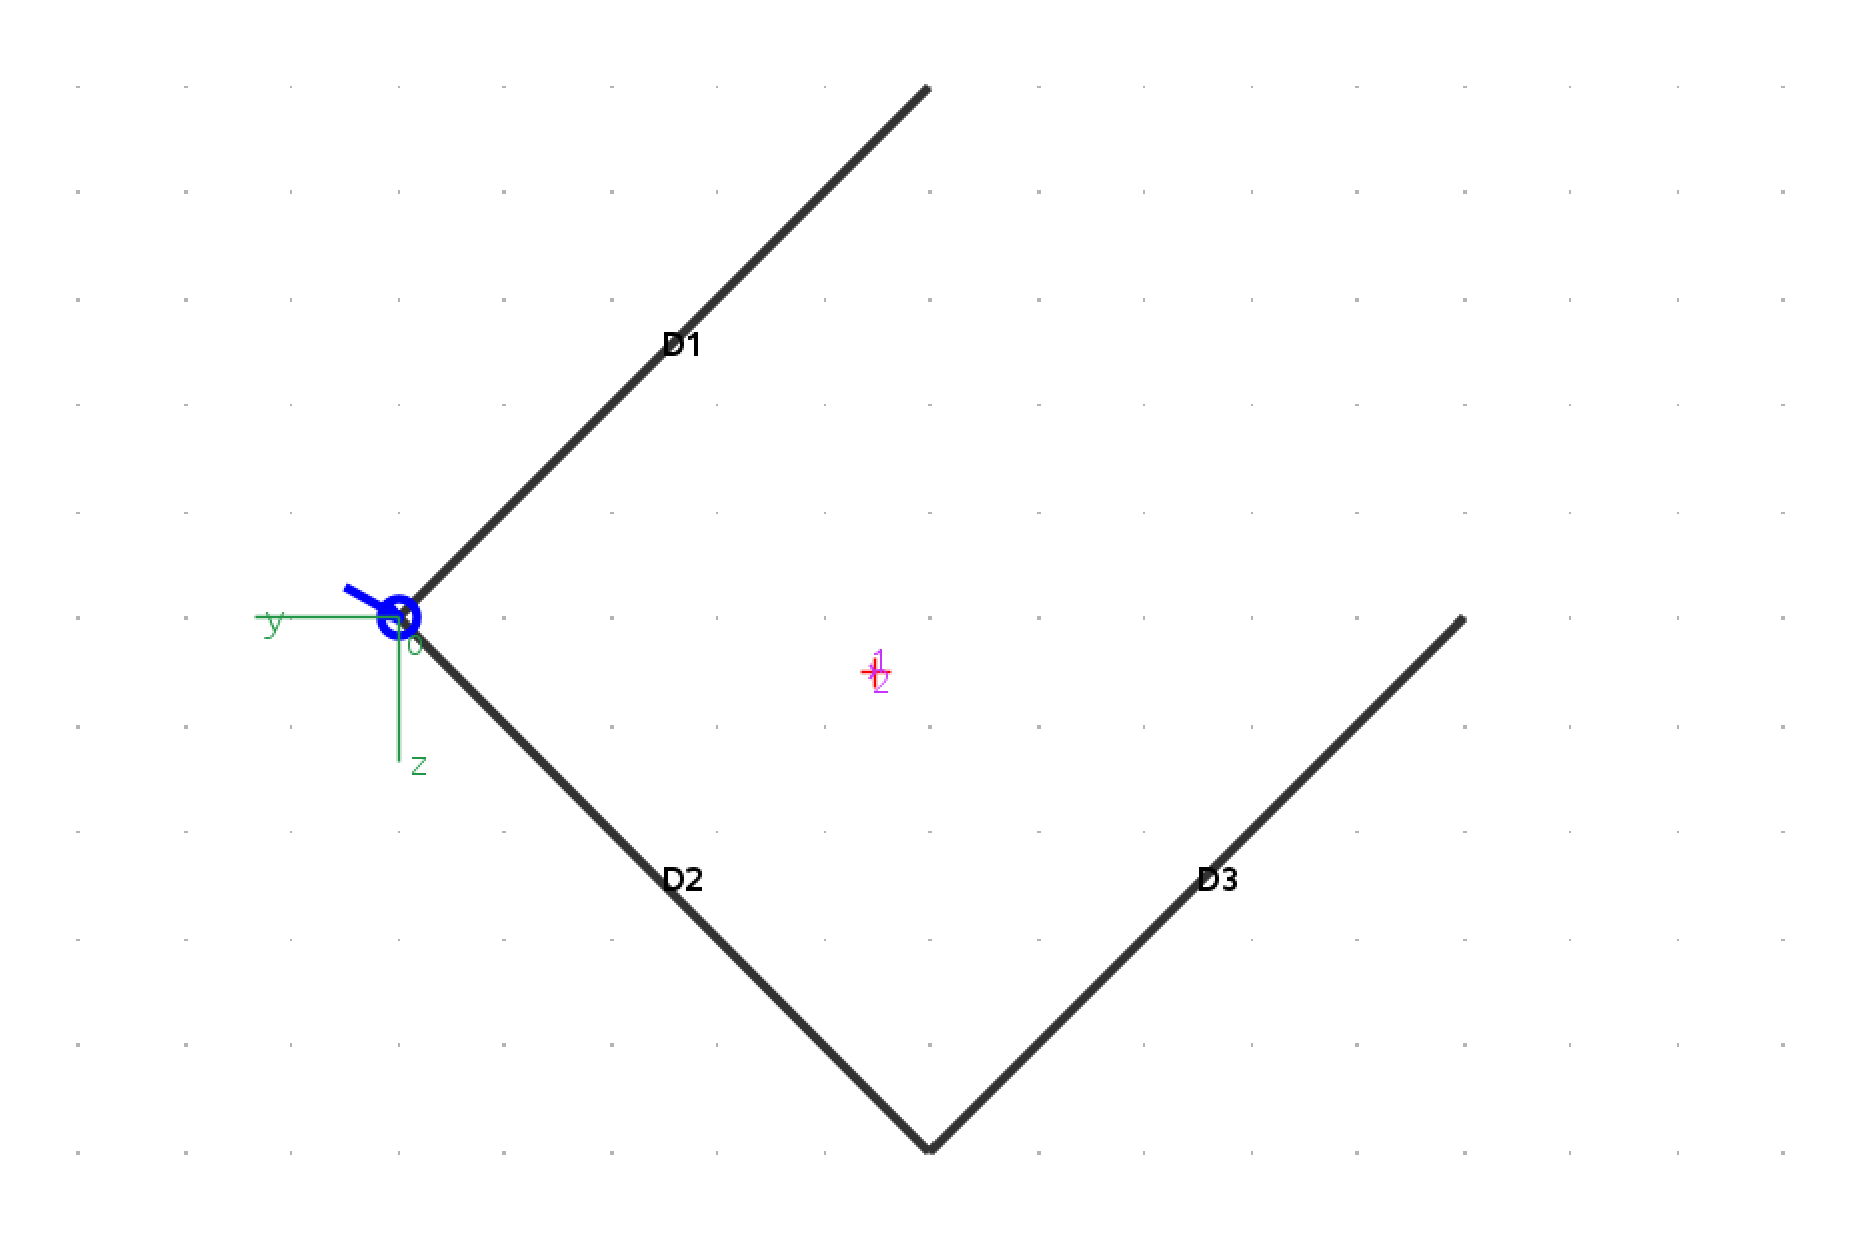
\includegraphics[width=0.7\linewidth]{./fig/TM2/WiSe2526nr8_1.png}
    \caption{TM2 WiSe~25/26, Nr.~8 im Programm}
    \label{fig:TM2WiSe2526Nr8_1}
\end{figure}

Bei dieser Aufgabe braucht man die $\sigma_x$-Berechnung. Um die Normalkraft hier richtig einzuberechnen
muss die Resultierende der Streckenlast über die halbe Länge berechnet werden, also: 
$R=0,1~\frac{\text{kN}}{cm}\cdot100~\text{cm}$.
Für die Kraft muss also $F_y=-500~\text{N}$, $F_z=300~\text{N}$ und $F_x=10000~\text{N}$ eingegeben werden.

Nach dem Aufruf der Berechnung werden noch ein paar Werte abgefragt. Für die ersten Drei muss Null eingetragen werden.
Man hätte auch keine Kraft platzieren können, die Normalkraft und Momente handisch ausrechnen können und diese dann in diese Felder eintragen können.
Das Ergebniss ist das gleiche.\\
Für $\Delta x$ muss $100~\text{cm}$ eingetragen werden, das ist der Abstand zwischen dem gezeichneten Schnitt und dem betrachteten Schnitt.
Das Programm rechnet dann also automatisch die Momente aus der Querkraft aus. Dieses Feature funktioniert natürlich nur, wenn zwischen dem gezeichneten und berechneten Schnitt
keine Weiteren Einflüsse wie Lager oder Kräfte Angreiffen, dann kommt man nicht darum herum $N$, $M_y$ und $M_z$ händisch auszurechnen und einzutragen.

Die Ergebnisse sind in Abbildung \ref{fig:TM2WiSe2526Nr8_2} dargestellt.

\begin{figure}[htbp]
    \centering
    \begin{subfigure}[t]{0.48\textwidth}
        \centering
        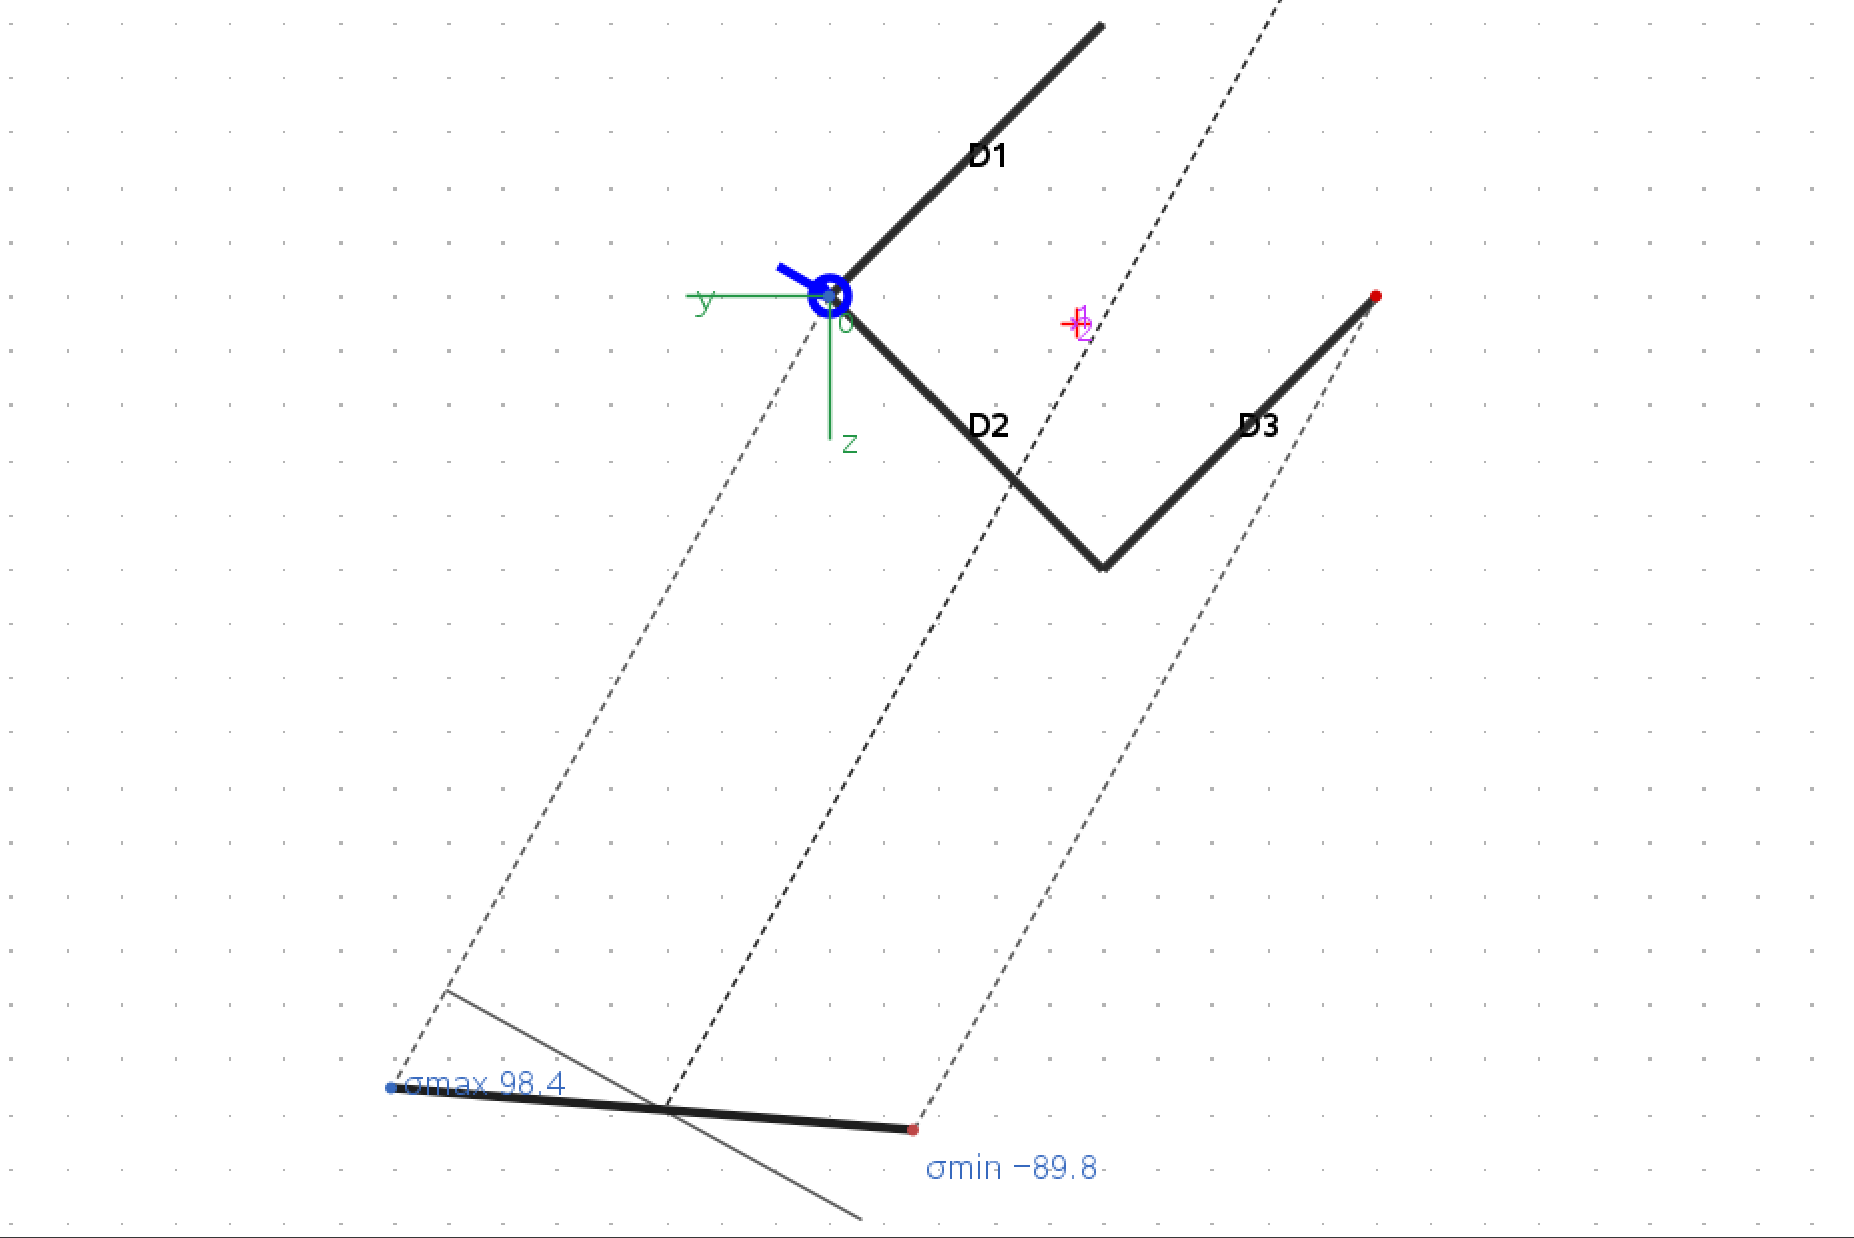
\includegraphics[width=\linewidth]{./fig/TM2/WiSe2526nr8_2.png}
        \caption{Spannungsverlauf}
    \end{subfigure}
    \hfill
    \begin{subfigure}[t]{0.48\textwidth}
        \centering
        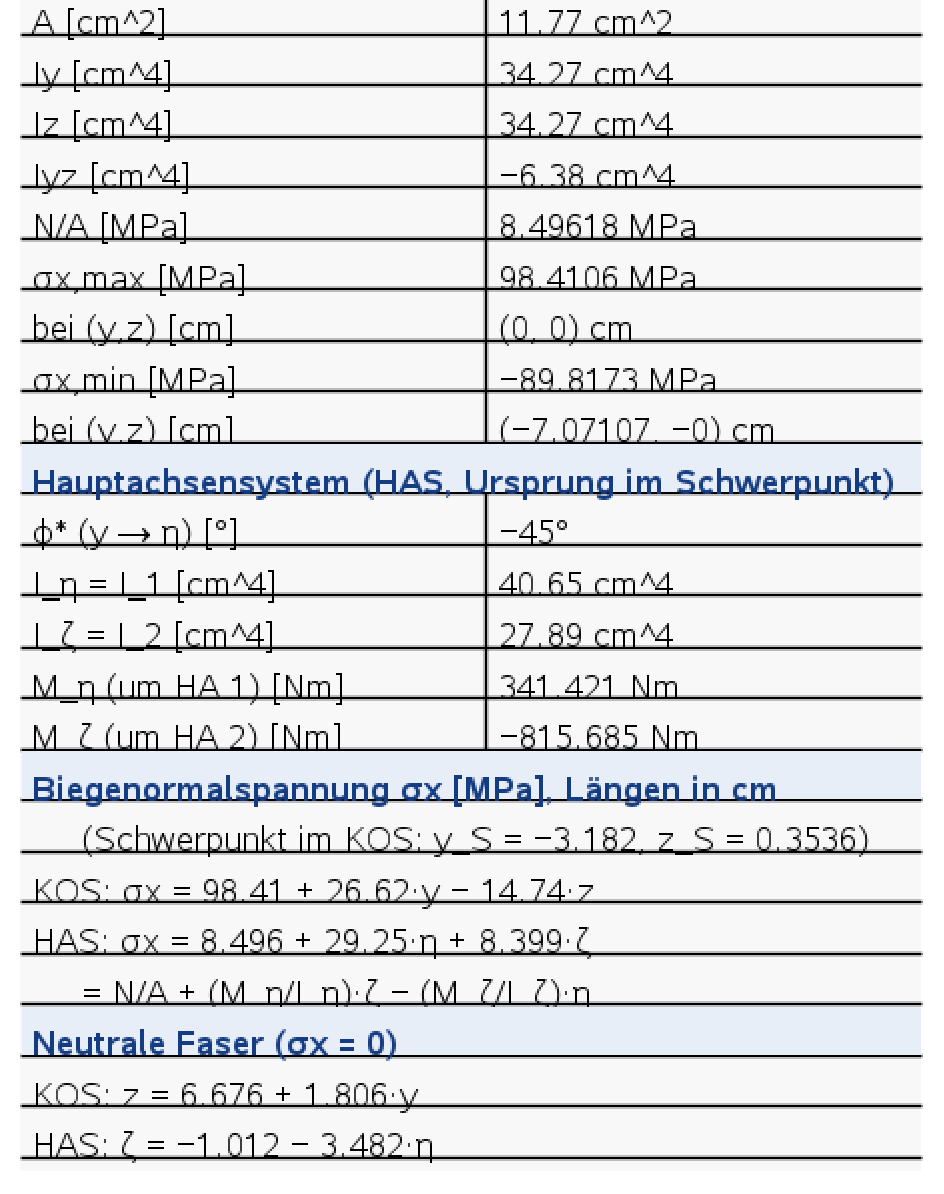
\includegraphics[width=\linewidth]{./fig/TM2/WiSe2526nr8_3.png}
        \caption{Tabellen übersicht}
    \end{subfigure}
    \caption{Lösung von TM2 WiSe~25/26, Nr.~8}
    \label{fig:TM2WiSe2526Nr8_2}
\end{figure}

Ich will anmereken, dass des öfteren bei Aufgaben Querschnittswerte gegeben sind, die nicht zur Bemaßung in der Zeichnung passen,
ob das absichtlich so ist konnte mir leider keiner sagen. Es ist also immer sinnvoll das einmal gegen zu prüfen und die Werte evtl. zu überschreiben.
Was die ISD-Musterlösung bei dieser Aufgabe gerechnet hat, ist mir nicht ganz klar. Meines Verständnisses nach wurde hier mit einem
Schwerpunkt für die Momente aus Normalkraft gerechnet, der genau in der Mitte des U profiels liegt, sodass die Normalkraft um die $y$-Achse kein Moment erzeugt.

\subsection{Schiefe Biegung/Kernfäche (TM2 WiSe21/22 Nr.~8)}



\subsection{MSK (TM2 WiSe 21/22 Nr.~3)}

Zu dieser Aufgabe gibt es eigentlich nicht besonders viel zu sagen, man gibt die gegebenen Werte ein und das Programm
füllt in grün die restlichen Werte auf (Abb.~\ref{fig:TM2WiSe2122Nr3_1}).

\begin{figure}[htbp]
    \centering
    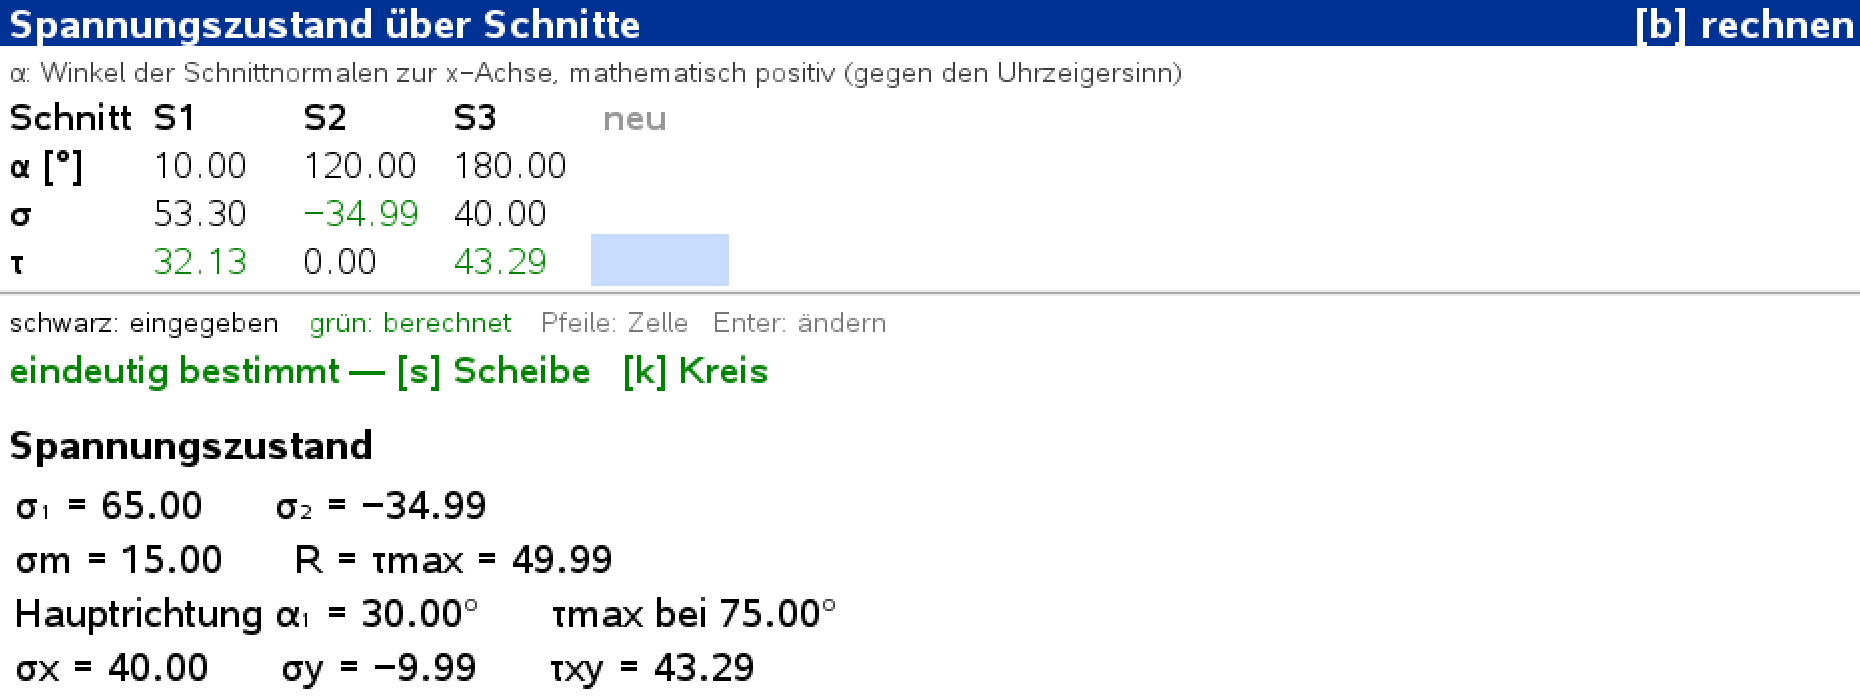
\includegraphics[width=0.7\linewidth]{./fig/TM2/WiSe2122nr3_1.png}
    \caption{TM2 WiSe~21/22, Nr.~3 im Programm}
    \label{fig:TM2WiSe2122Nr3_1}
\end{figure}

Danach bekommt man mit den Tasten \taste{s} und \taste{k} die beiden wichtigen Ansichten (Abb.~\ref{fig:TM2WiSe2122Nr3_2}).


\begin{figure}[htbp]
    \centering
    \begin{subfigure}[t]{0.48\textwidth}
        \centering
        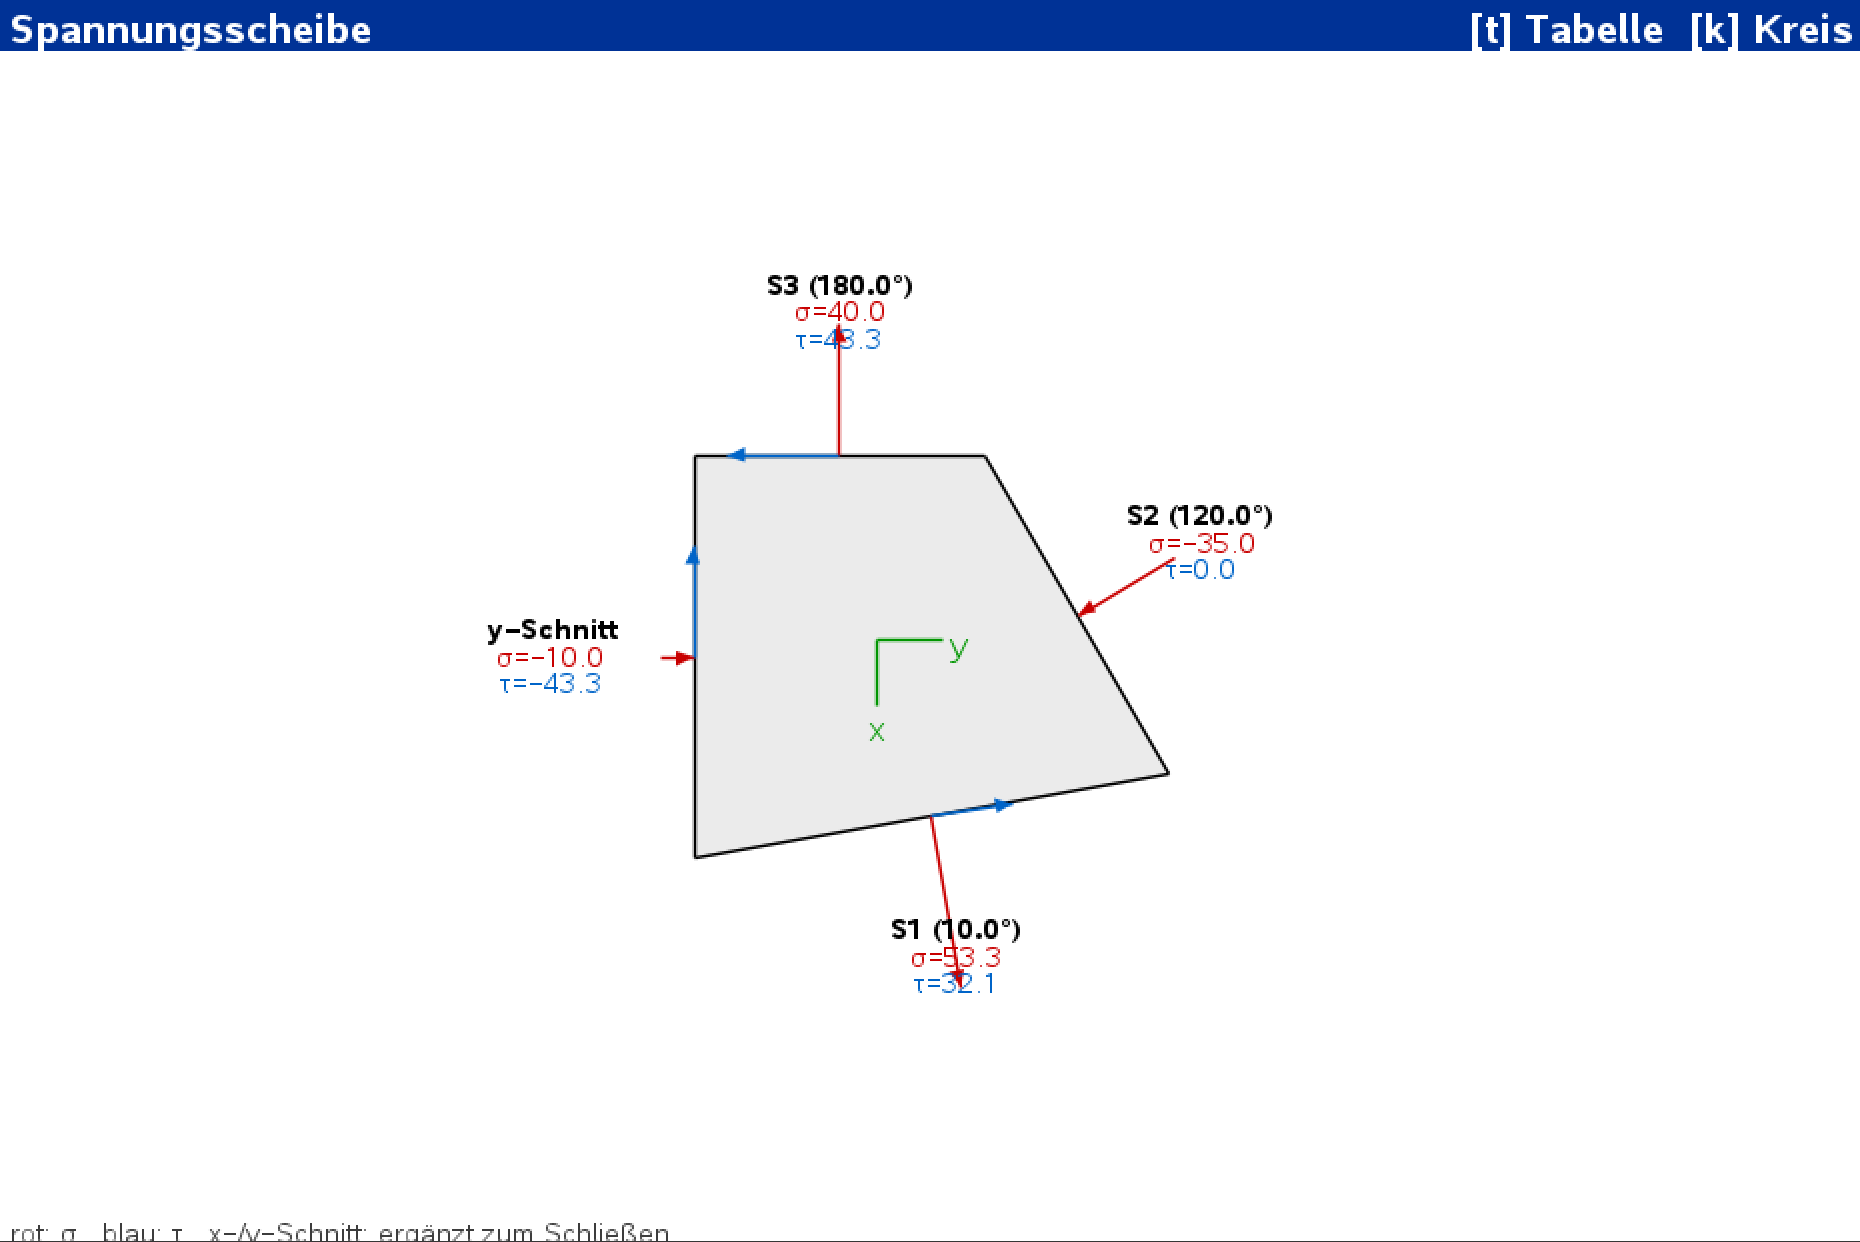
\includegraphics[width=\linewidth]{./fig/TM2/WiSe2122nr3_2.png}
        \caption{Spannungs-Scheibe}
    \end{subfigure}
    \hfill
    \begin{subfigure}[t]{0.48\textwidth}
        \centering
        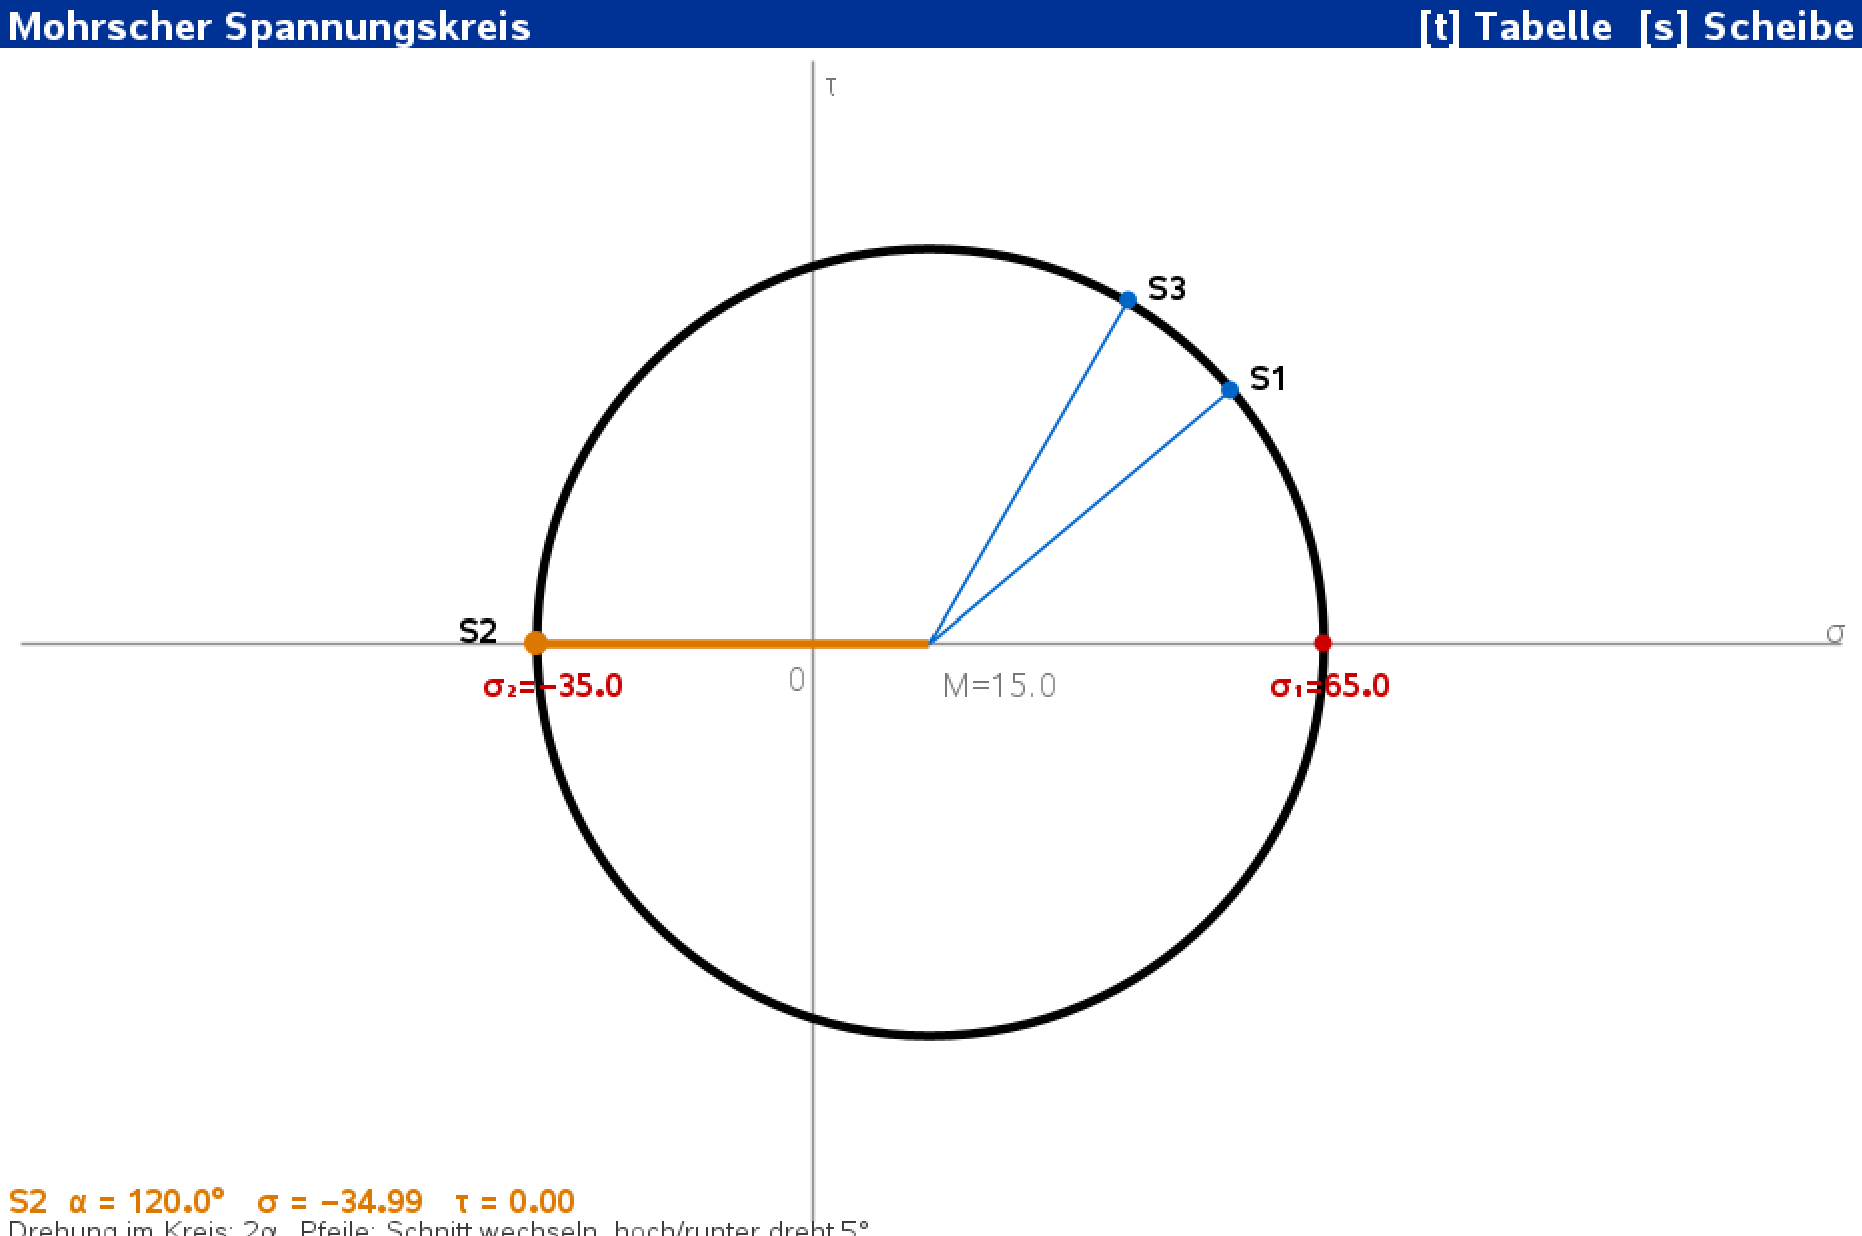
\includegraphics[width=\linewidth]{./fig/TM2/WiSe2122nr3_3.png}
        \caption{Spannungs-Kreis}
    \end{subfigure}
    \caption{Lösung von TM2 WiSe~21/22, Nr.~3}
    \label{fig:TM2WiSe2122Nr3_2}
\end{figure}

Falls bei einer Aufgabe nach dem Winkel eines Schnitts gefragt wird und das Programm zwei Winkel ausgibt, muss natürlich
geprüft werden, welcher Winkel eher zur Skizze passt.

\subsection{Schubspannung und SMP (TM2 SoSe 24 Nr.~8)}

\subsection{Verwölbung (TM2 SoSe 20 Nr.~9)} eingebunden.
% Hier keine \usepackage-Zeilen: Pakete stehen in der Praeambel von Anleitung.tex.
% Abbildungen mit [htbp]: LaTeX setzt sie dann dorthin, wo Platz ist. Im Text deshalb immer
% mit Abb.~\ref{...} auf sie verweisen, nicht mit "unten" oder "folgendermaßen".


\part{Beispiele}

In diesem Teil will ich anhand typischer Klausuraufgaben etwas genauer beschreiben, wie man das
Programm am besten verwendet, zumindest so, wie ich es für sinnvoll halte.

Die Screenshots habe ich in der PC-Ansicht gemacht, weil dort viele Dinge besser erkennbar sind.
Auf dem Taschenrechner selbst sollte mit Zoom aber auch alles erkennbar sein.

\section{TM1}
\subsection{WiSe~21/22}
\subsubsection{Geschlossenes System (Nr.~2)}
Bei dieser Aufgabe gibt es ein paar Besonderheiten bei der Eingabe, deshalb stelle ich sie hier vor.
Im Programm sieht das Tragwerk aus wie in Abb.~\ref{fig:WiSe2122nr2_1}.

\begin{figure}[htbp]
    \centering
    \begin{subfigure}[t]{0.48\textwidth}
        \centering
        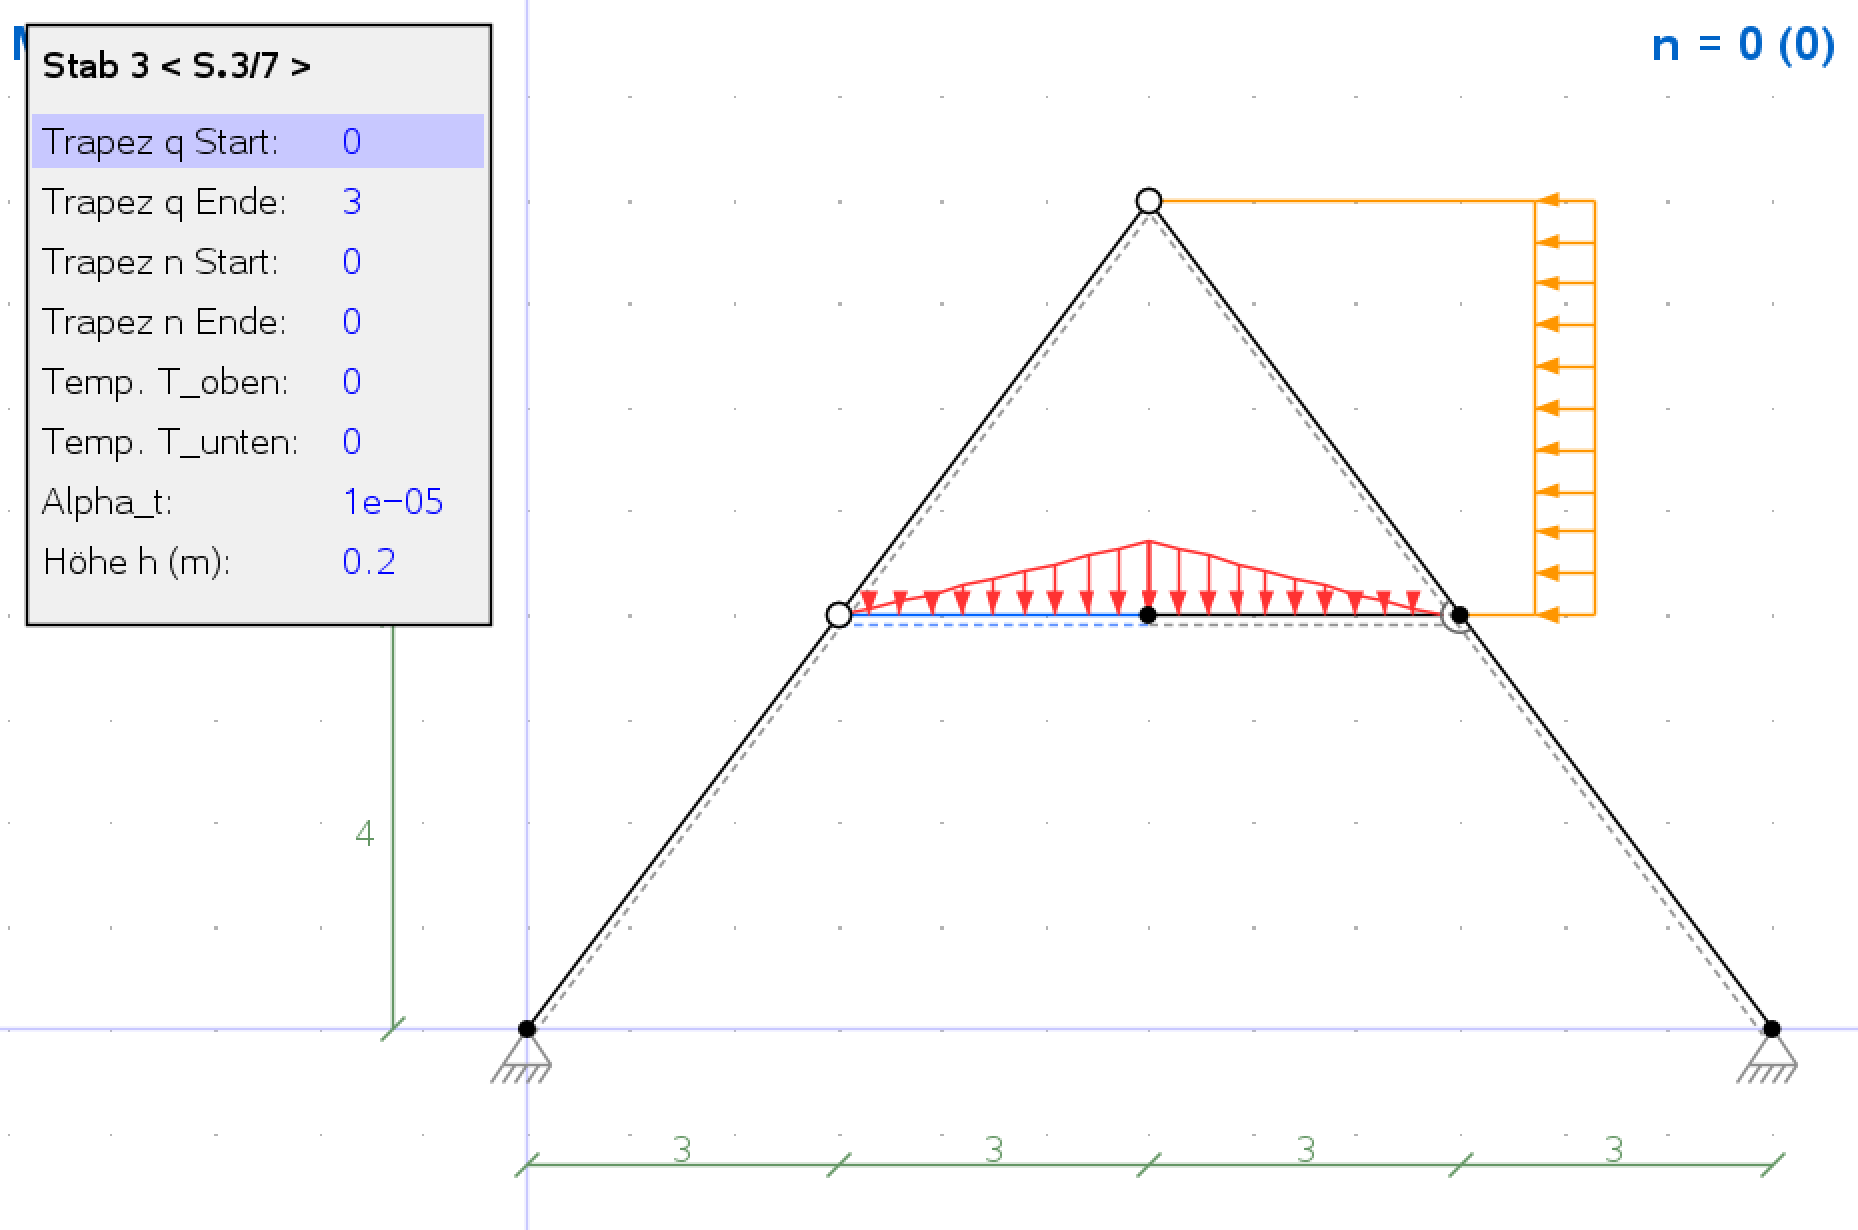
\includegraphics[width=\linewidth]{./fig/TM1/WiSe2122nr2_1.png}
        \caption{Trapezlast auf der linken Hälfte des Mittelstabs}
    \end{subfigure}
    \hfill
    \begin{subfigure}[t]{0.48\textwidth}
        \centering
        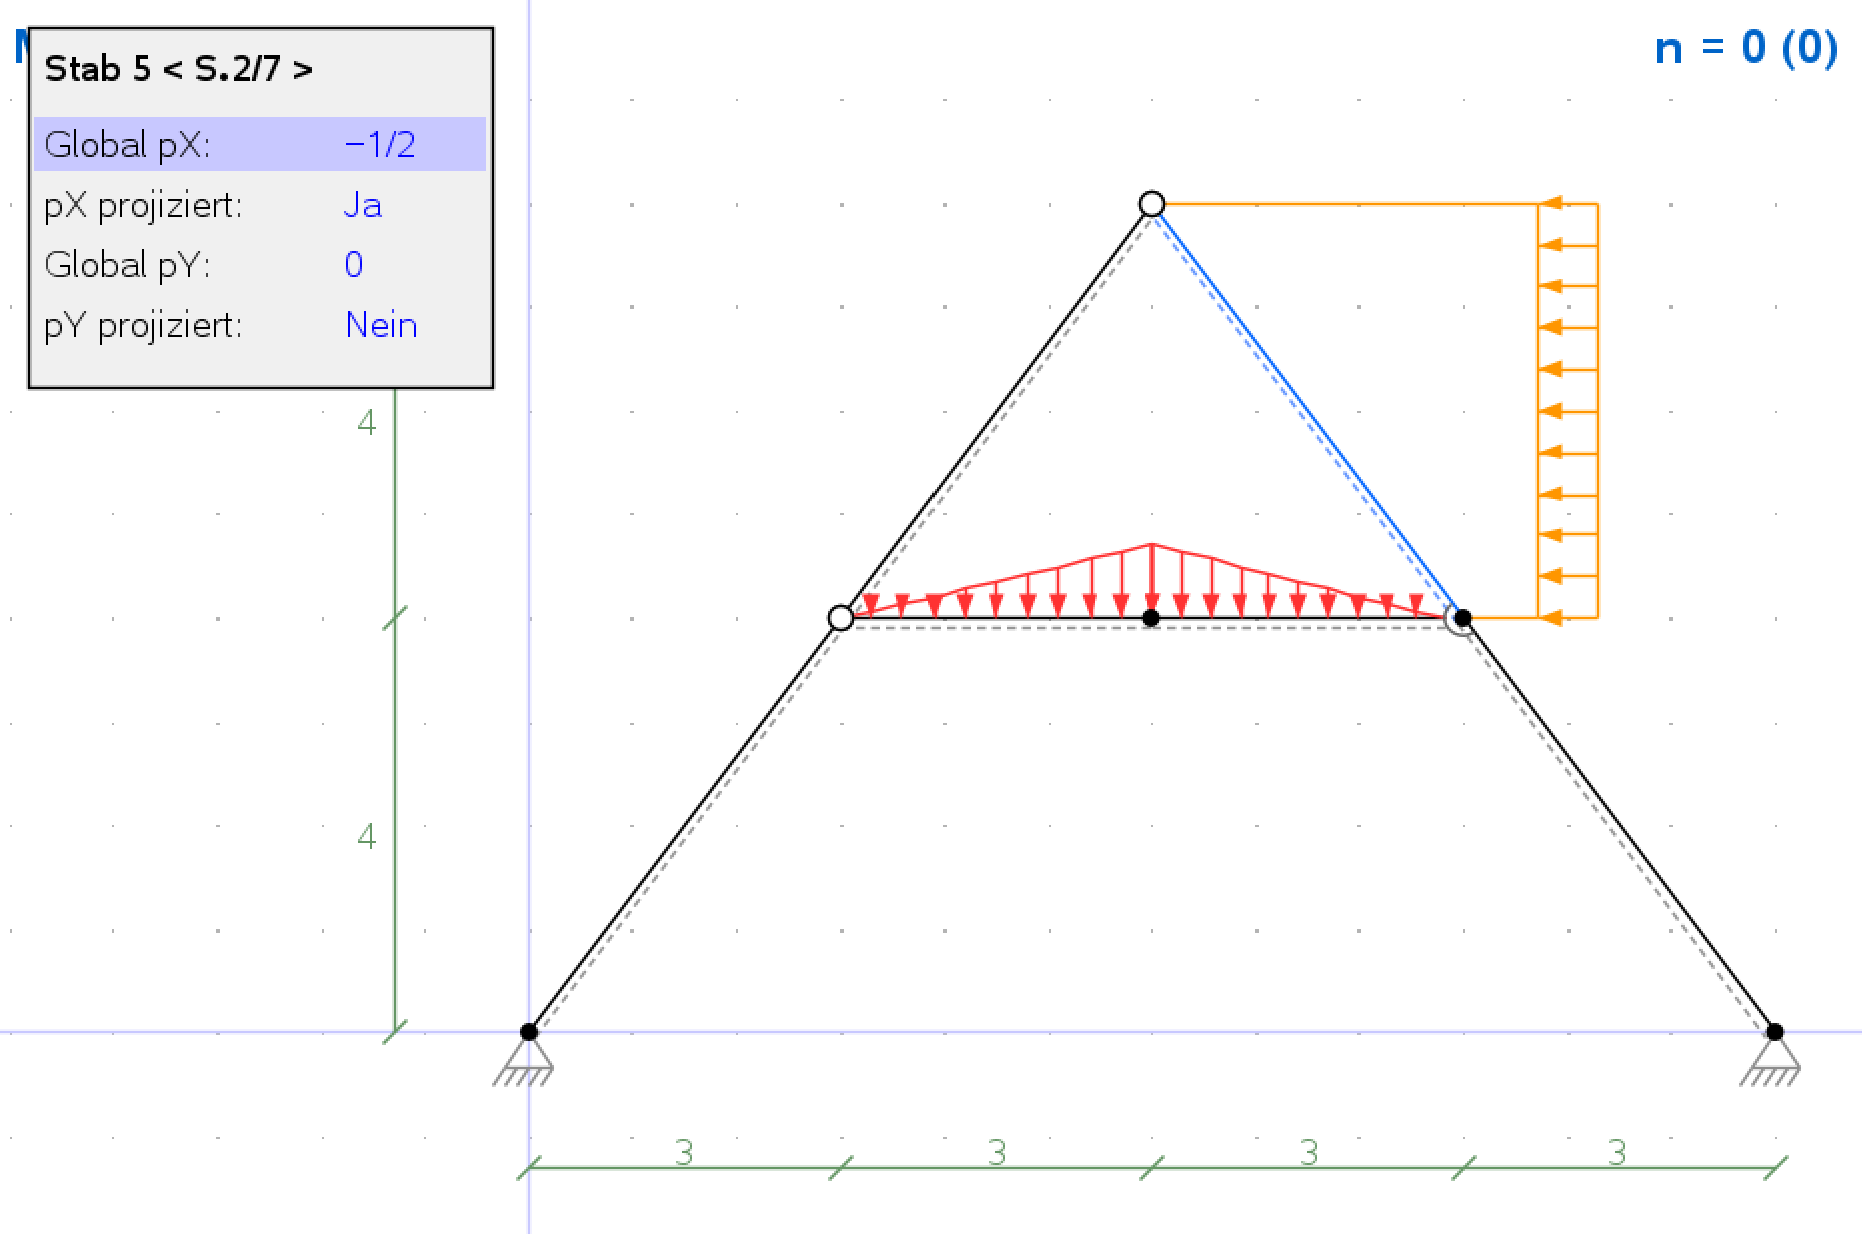
\includegraphics[width=\linewidth]{./fig/TM1/WiSe2122nr2_2.png}
        \caption{globale Streckenlast am oberen rechten Stab}
    \end{subfigure}
    \caption{WiSe~21/22, Nr.~2 im Programm}
    \label{fig:WiSe2122nr2_1}
\end{figure}

Den Stab in der Mitte müsst ihr im Programm teilen. Die Last auf ihm ist dreieckförmig mit der
Spitze in der Mitte, eine Trapezlast geht aber immer über einen ganzen Stab. Jede Hälfte bekommt
deshalb ihre eigene Trapezlast, die linke von $0$ auf $3$, die rechte von $3$ auf $0$
(Abb.~\ref{fig:WiSe2122nr2_1}a). Der neue Knoten in der Mitte bleibt biegesteif.

Die Streckenlast am schrägen Stab gebt ihr am einfachsten als globale Last ein
(Abb.~\ref{fig:WiSe2122nr2_1}b). In der Aufgabe ist sie auf die senkrechte Projektion des Stabes
bezogen, deshalb muss \emph{pX projiziert} auf \emph{Ja} stehen. Negativ ist sie, weil sie global
gesehen entgegen der $x$-Achse wirkt, also nach links.

Nach dem Berechnen könnt ihr das LGS, das zur Explosionsansicht (Abb.~\ref{fig:WiSe2122nr2_2})
gehört, über die zweite Seite des Obermenüs (\emph{LGS-Matrix}) in den Taschenrechner exportieren
(Abb.~\ref{fig:WiSe2122nr2_3}). Die Gleichungen stehen dann lesbar in \code{lgs}, die Lösung
bekommt ihr zum Beispiel mit \code{ggw\_x = ggw\_a$^{-1}$*ggw\_b}
(Abschnitt~\ref{sec:lgs-matrix}).

\begin{figure}[htbp]
    \centering
    \begin{subfigure}[t]{0.48\textwidth}
        \centering
        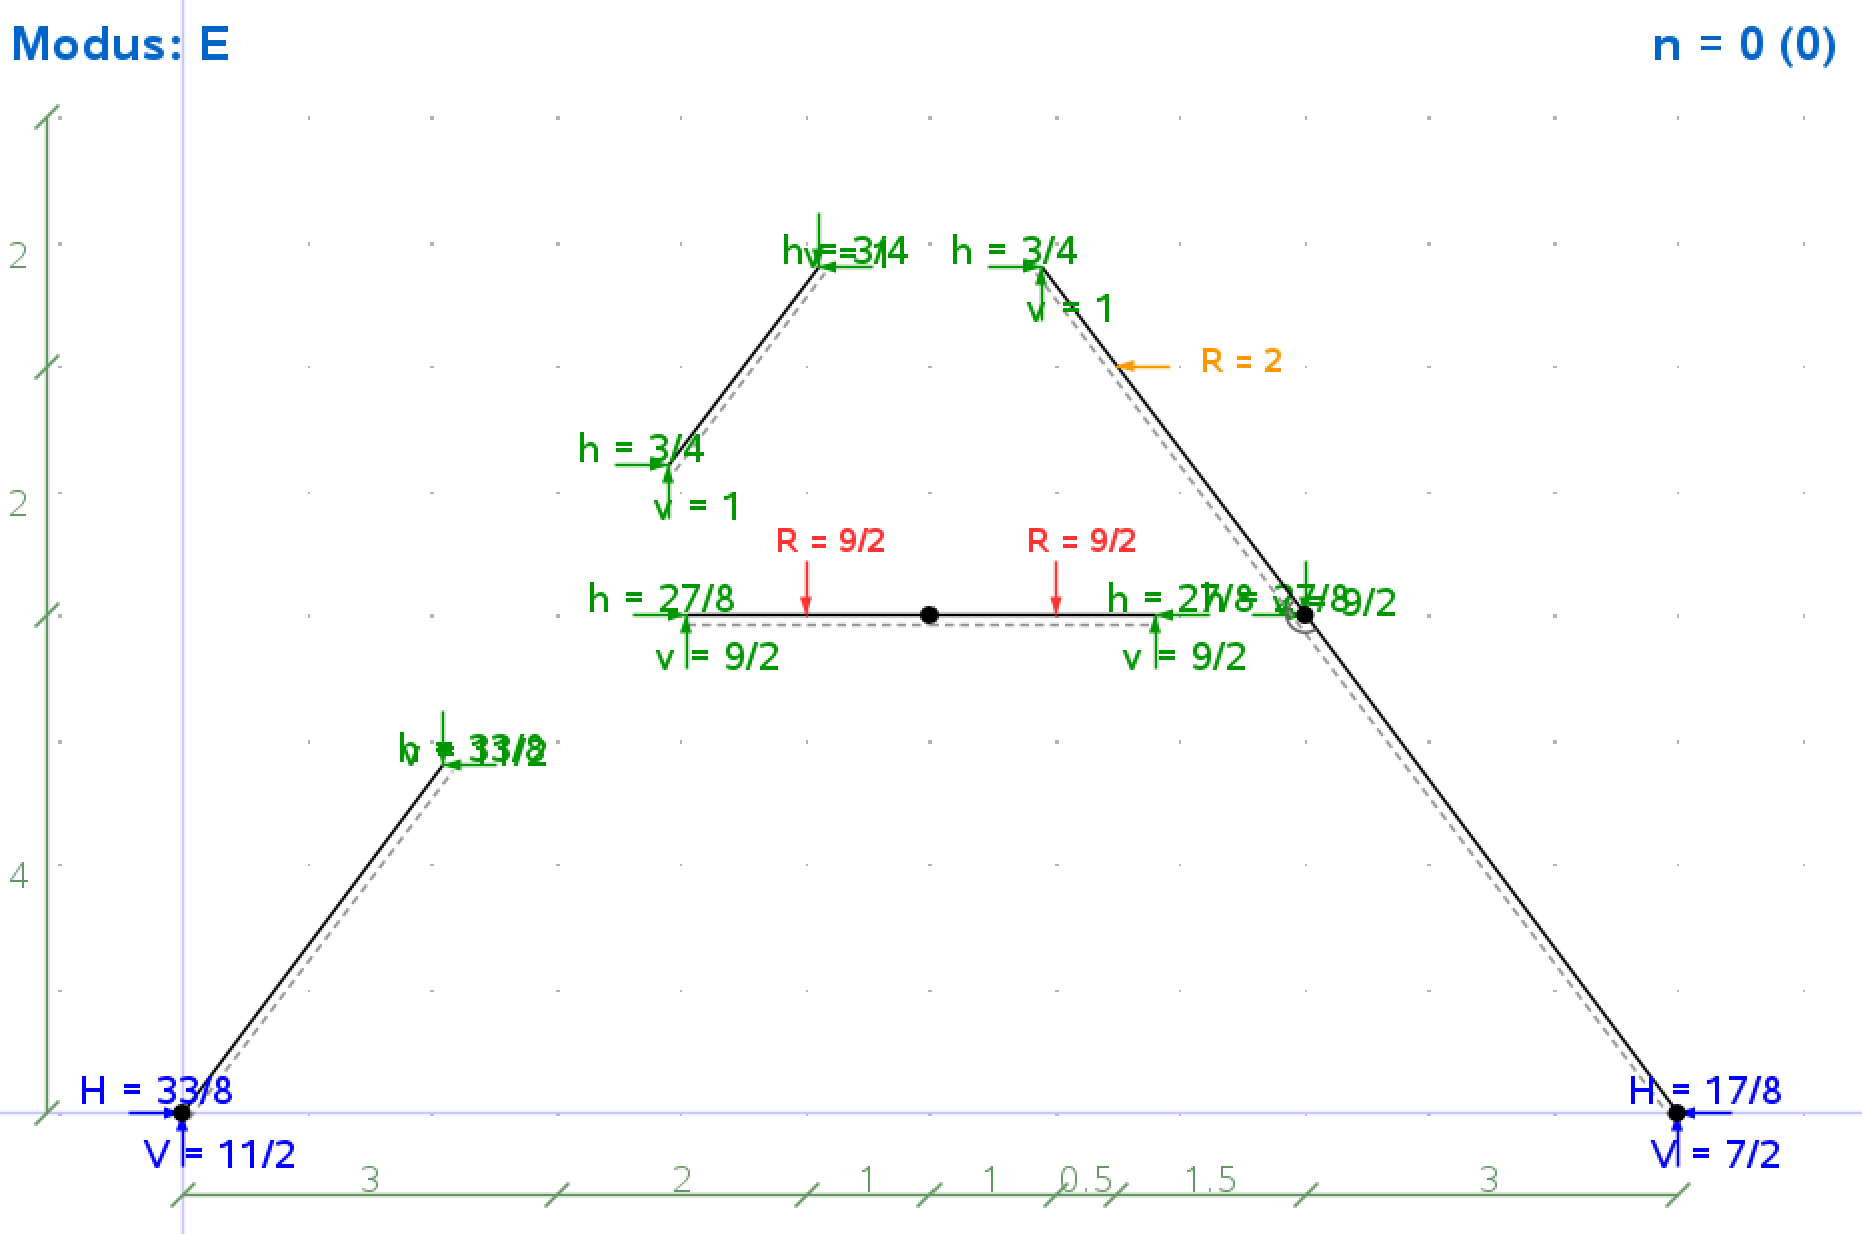
\includegraphics[width=\linewidth]{./fig/TM1/WiSe2122nr2_5.png}
        \caption{Seite~1: Ergebnisse in ihrer wirklichen Richtung}
    \end{subfigure}
    \hfill
    \begin{subfigure}[t]{0.48\textwidth}
        \centering
        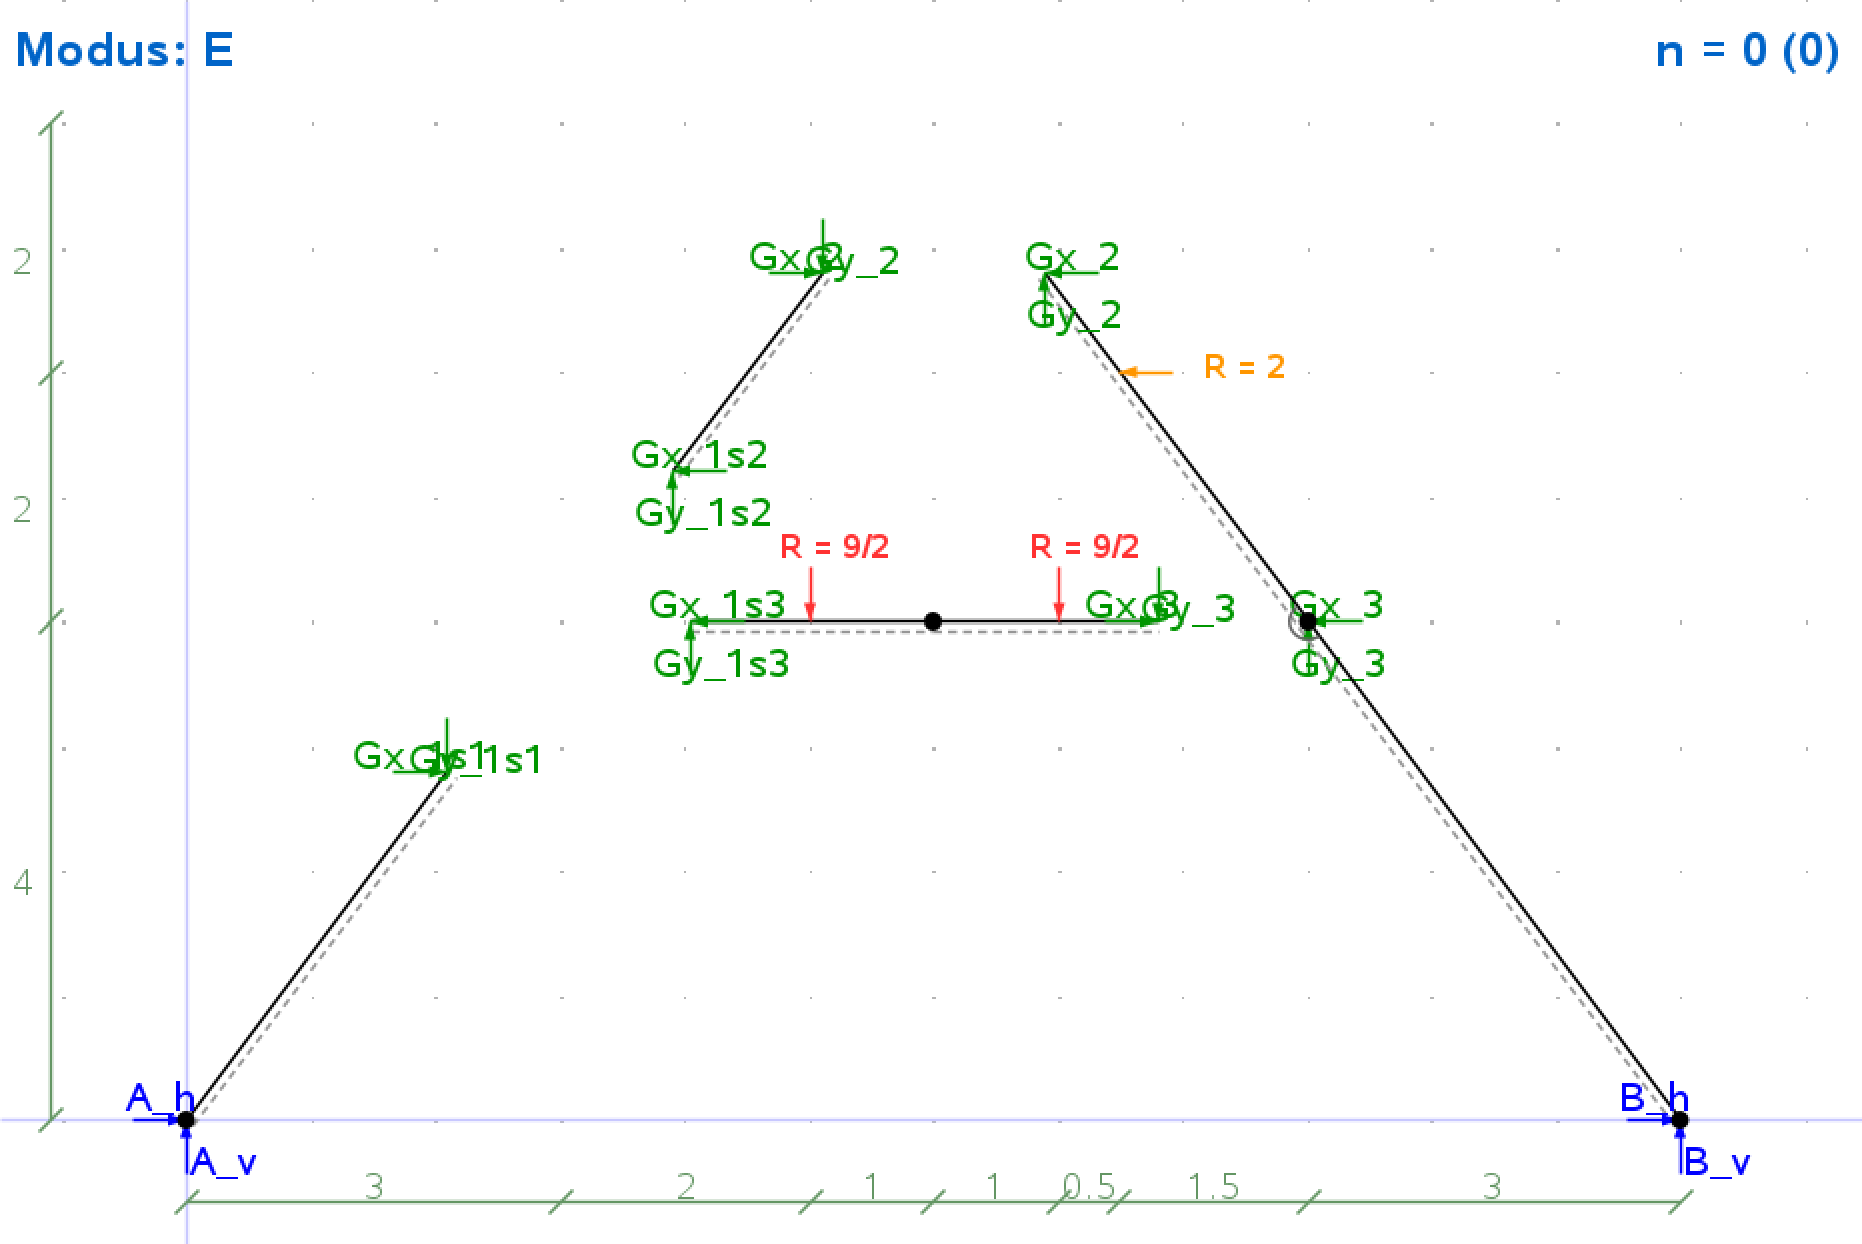
\includegraphics[width=\linewidth]{./fig/TM1/WiSe2122nr2_6.png}
        \caption{Seite~2: Unbekannte in positiver Richtung}
    \end{subfigure}
    \caption{WiSe~21/22, Nr.~2: Explosionsansicht (E-Modus)}
    \label{fig:WiSe2122nr2_2}
\end{figure}

\begin{figure}[htbp]
    \centering
    \begin{subfigure}[t]{0.48\textwidth}
        \centering
        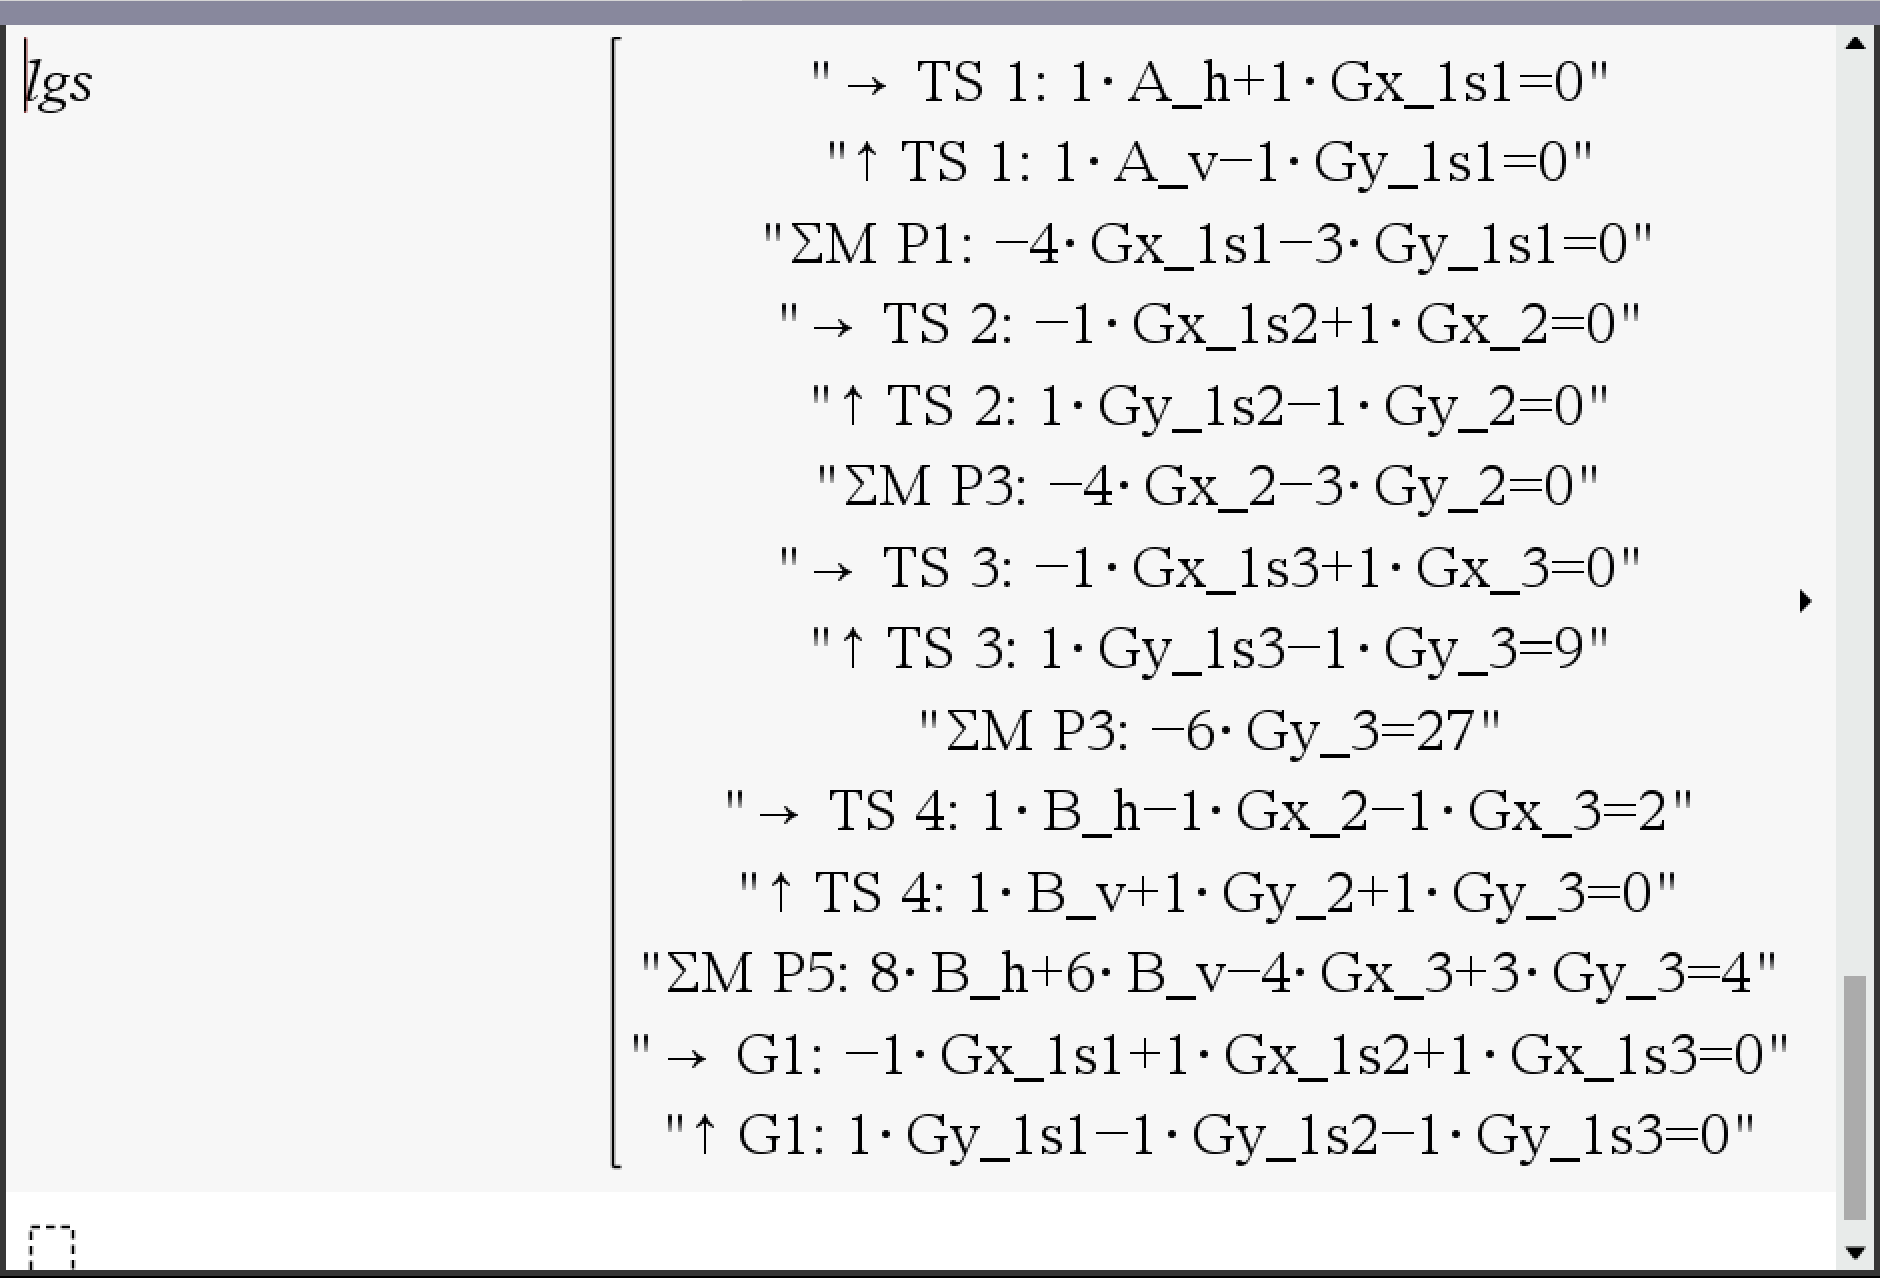
\includegraphics[width=\linewidth]{./fig/TM1/WiSe2122nr2_3.png}
        \caption{exportierte Gleichungen \code{lgs}}
    \end{subfigure}
    \hfill
    \begin{subfigure}[t]{0.48\textwidth}
        \centering
        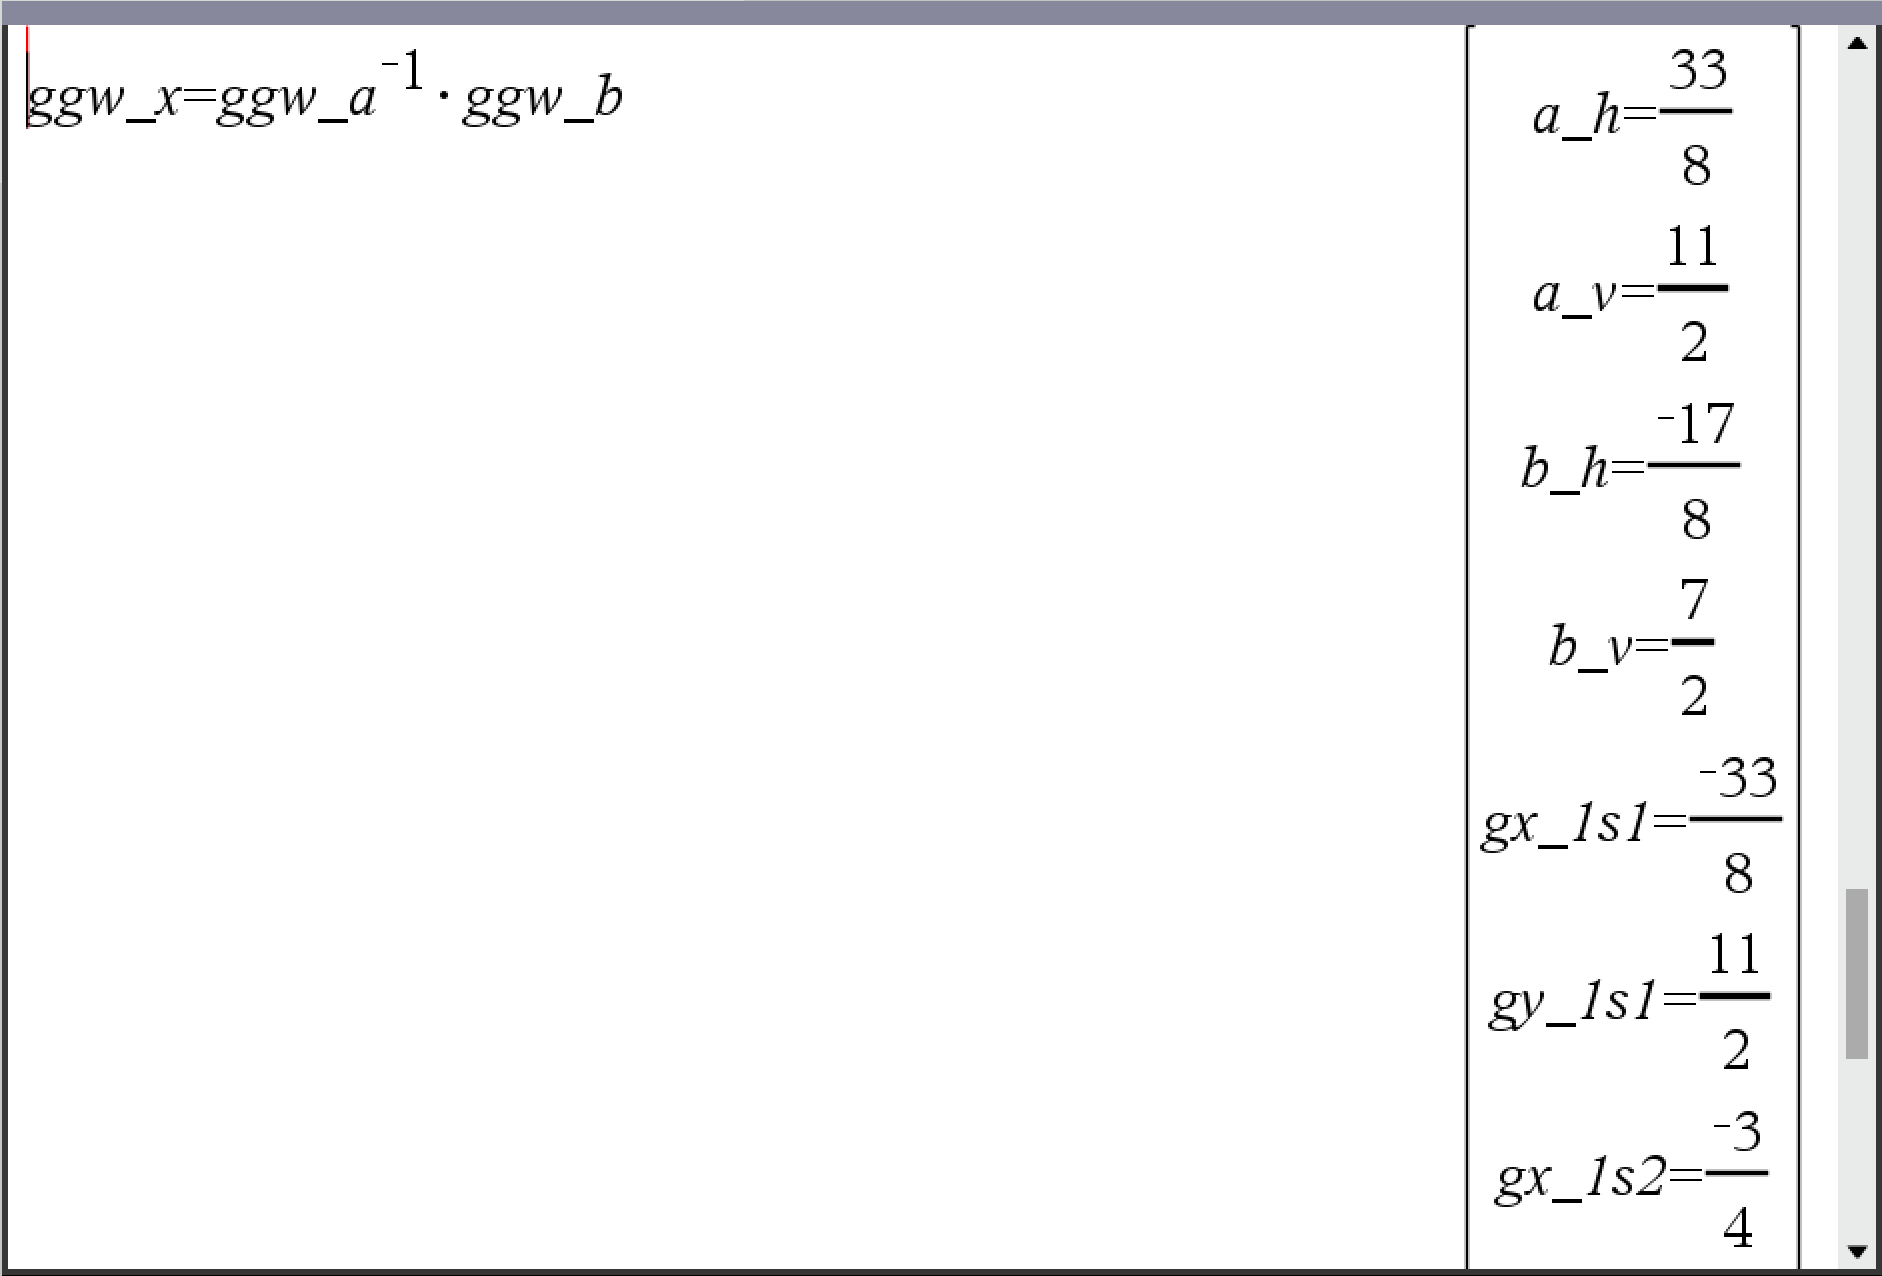
\includegraphics[width=\linewidth]{./fig/TM1/WiSe2122mr2_4.png}
        \caption{Lösung mit \code{ggw\_x}}
    \end{subfigure}
    \caption{WiSe~21/22, Nr.~2: exportiertes LGS}
    \label{fig:WiSe2122nr2_3}
\end{figure}

Die Explosionsansicht kann manchmal etwas unübersichtlich sein. Wenn ihr nah genug heranzoomt,
sollte aber trotzdem alles erkennbar sein. Die Ergebnisse müsst ihr natürlich nicht in dieser
Vektorform aufschreiben, nur ihr Inhalt zählt.

An dieser Stelle will ich anmerken, dass meist nur bei Systemen mit einem geschlossenen Ring wie
diesem nach allen Gelenk- und Auflagerkräften gefragt wird. Bei offenen Systemen ohne Ring wird oft
nur nach den Auflagerkräften gefragt. Das exportierte LGS liefert dann zwar auch die richtige Lösung, ist aber
meist mehr, als ihr braucht. Den Punkt, um den das Programm die Momentensumme eines Teilsystems
bildet, seht ihr, wenn ihr in der Explosionsansicht mit der Maus über das Teilsystem fahrt
(\emph{Hover}).

Die Zustandslinien, also die Verläufe der Schnittgrößen, zeichnet euch das Programm mit den Tasten
\taste{n}, \taste{q} und \taste{m}, die könnt ihr einfach abzeichnen. Falls ihr Randwerte schlecht
erkennt, fahrt mit der Maus über den jeweiligen Stab, dann zeigt das Programm nur noch diesen Stab
mit seinen Randwerten an.

\subsubsection{Qualitavtive Verläufe im symbolischen Modus (Nr.~4)}

Um meinen den oben genannten Punkt zum symbolischen Modus zu verdeutlichen will ich hier kurz auf Teilaufgabe b) eingehen.
Das System und der Querkraftverlauf sind in Abbildung~\ref{fig:TM1WiSe2122Nr4} dargestellt.

\begin{figure}[htbp]
    \centering
    \begin{subfigure}[t]{0.48\textwidth}
        \centering
        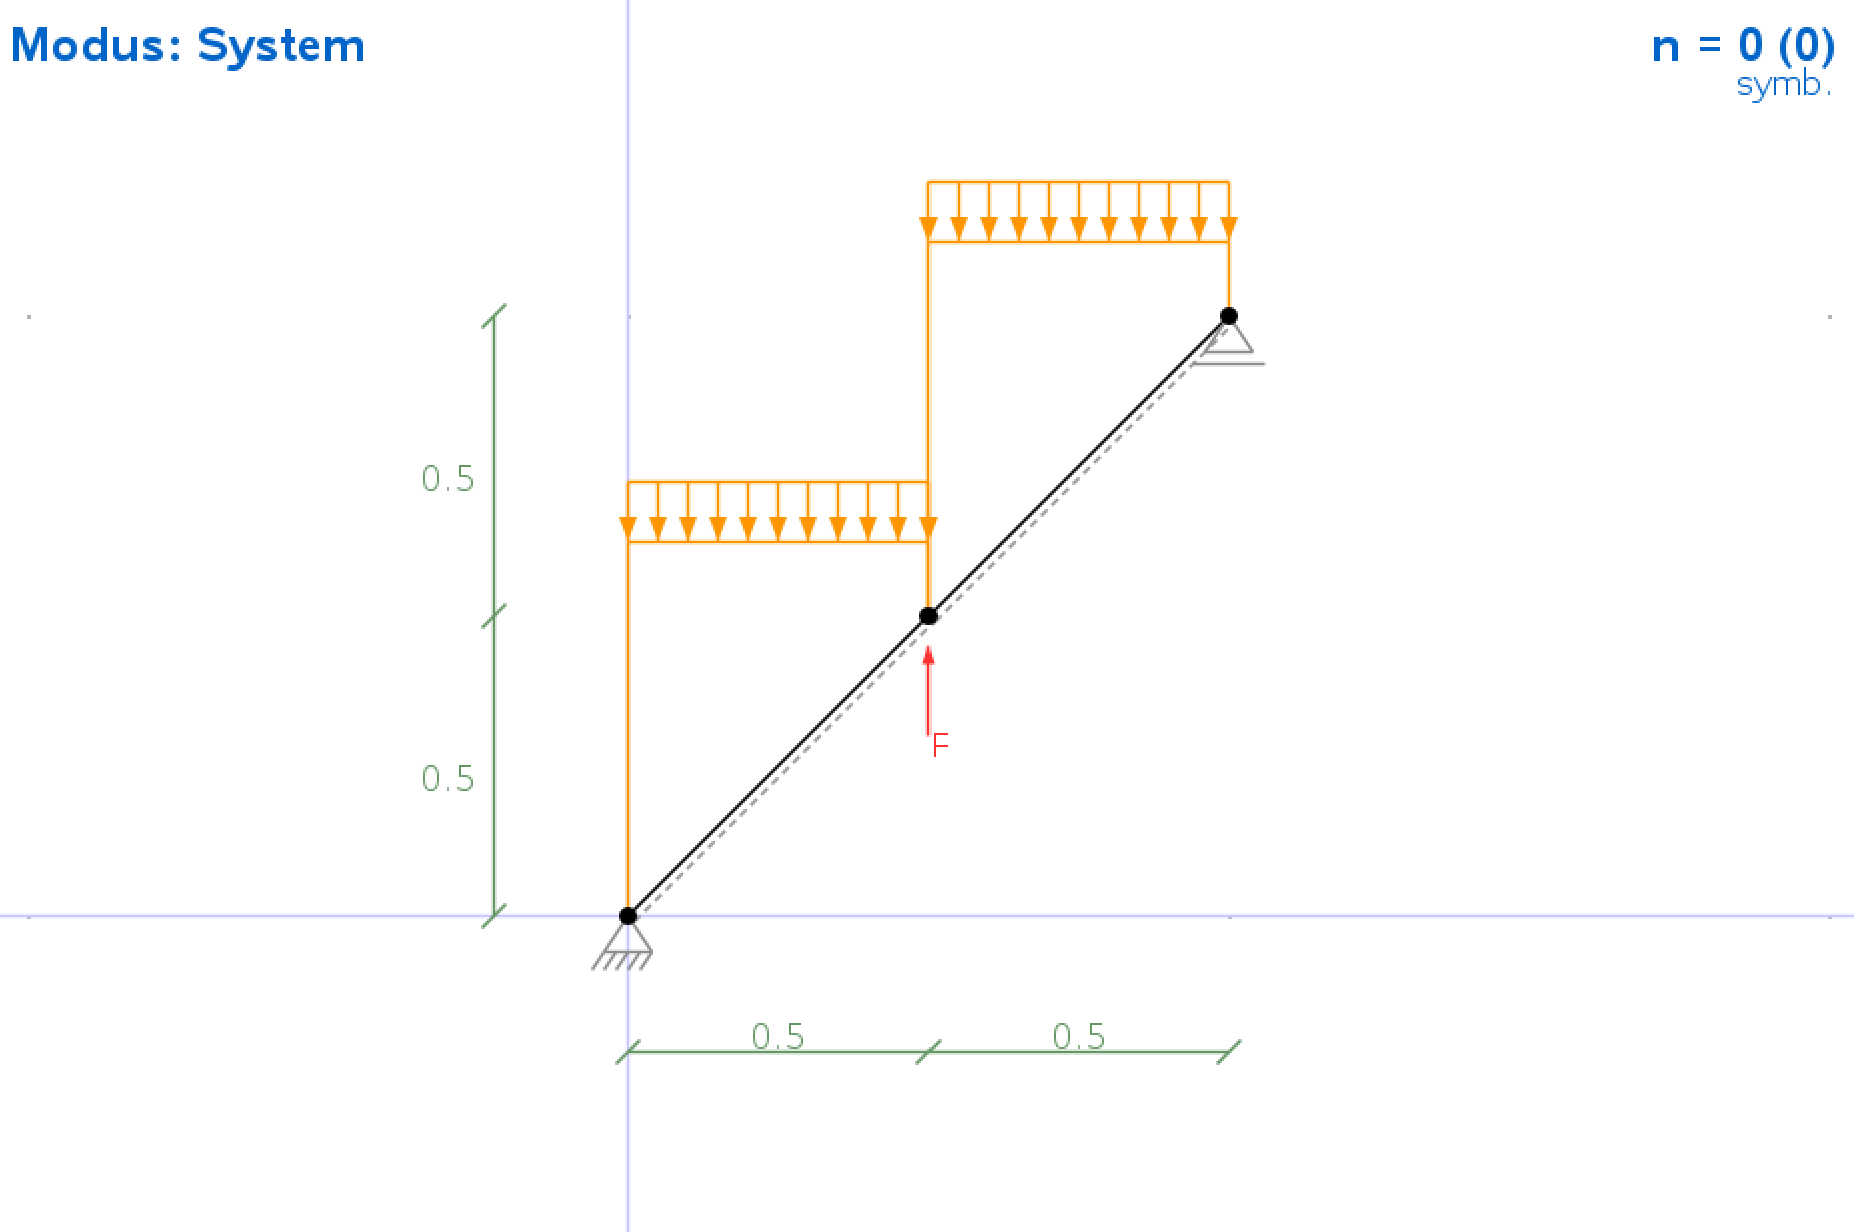
\includegraphics[width=\linewidth]{./fig/TM1/WiSe2122nr4_1.png}
        \caption{System}
    \end{subfigure}
    \hfill
    \begin{subfigure}[t]{0.48\textwidth}
        \centering
        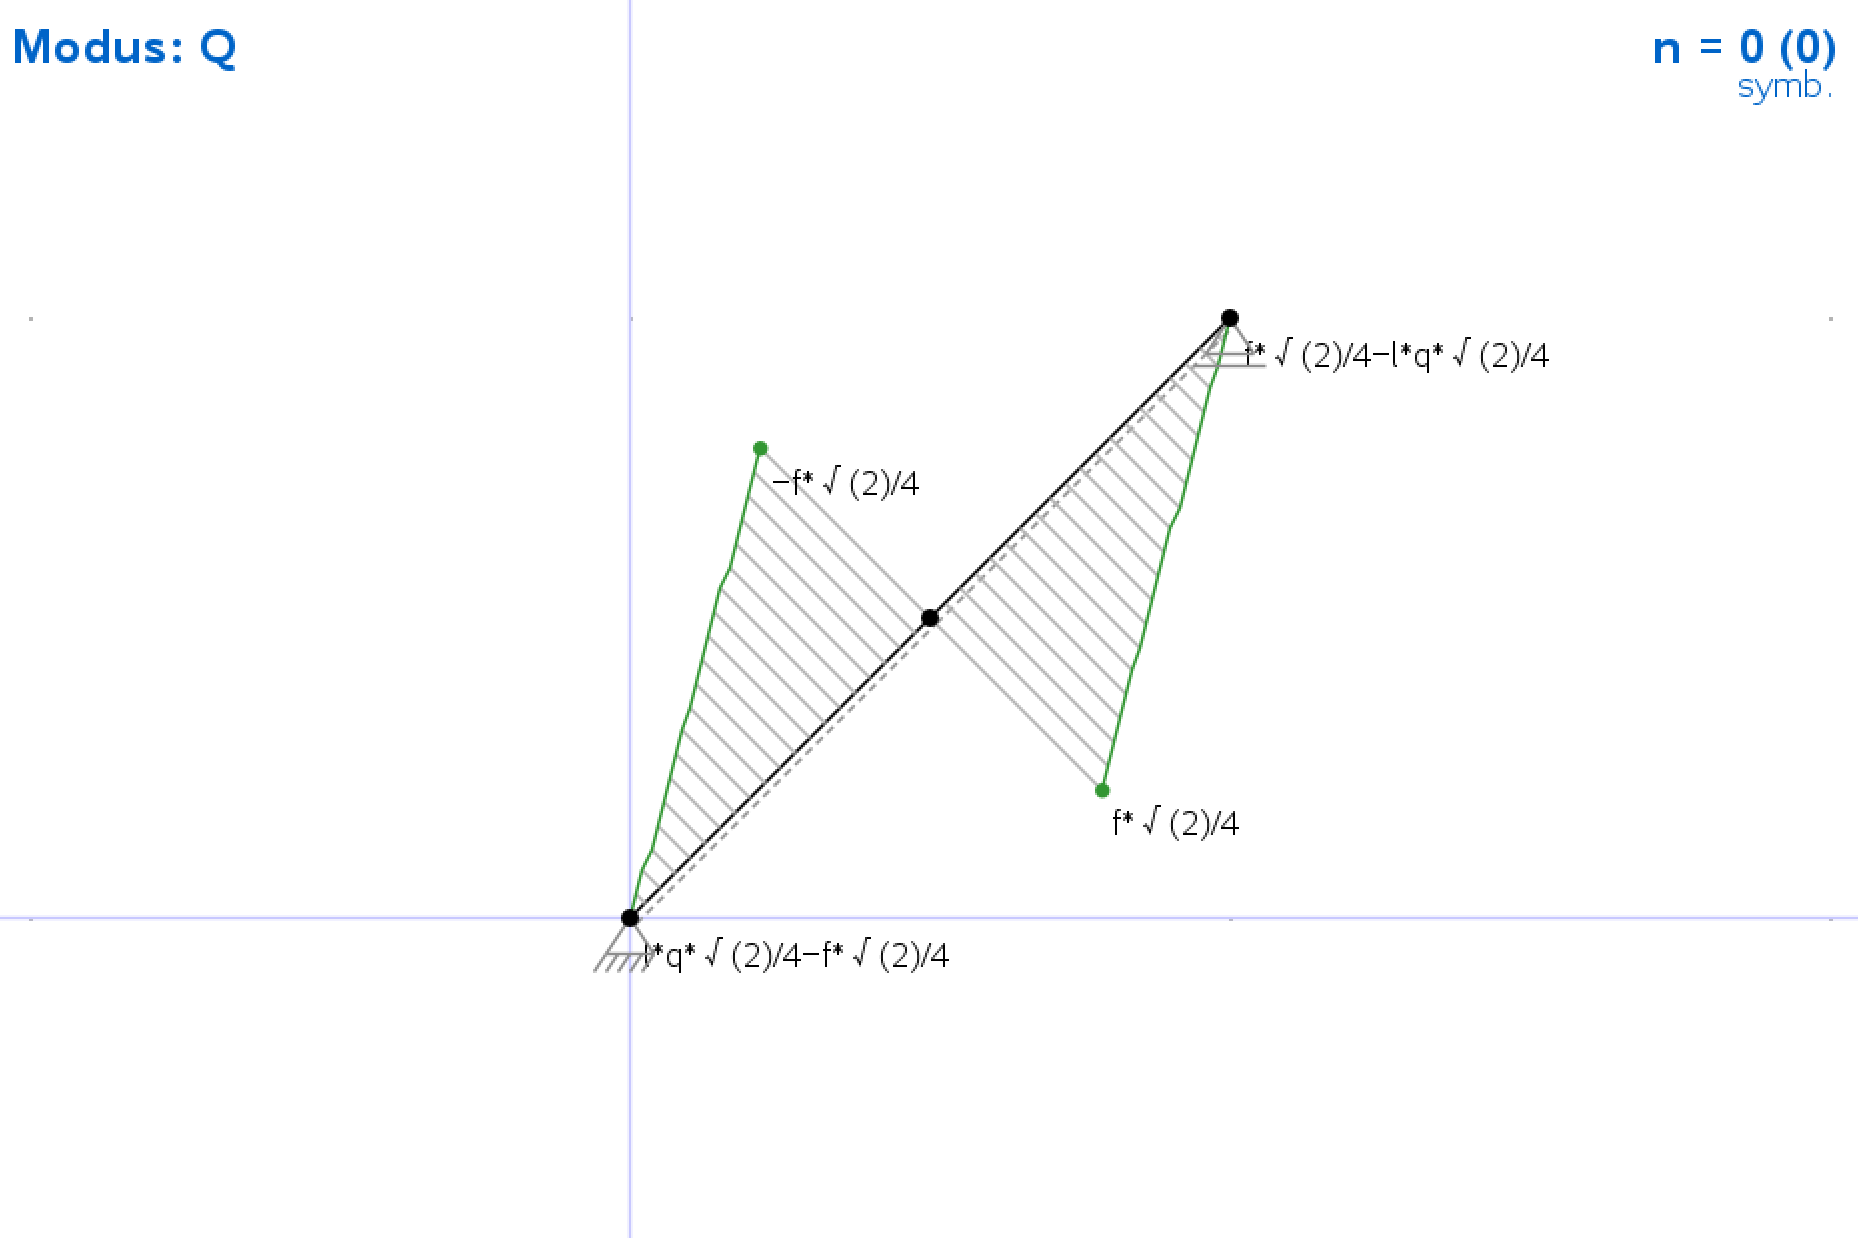
\includegraphics[width=\linewidth]{./fig/TM1/WiSe2122nr4_2.png}
        \caption{Querkraftverlauf}
    \end{subfigure}
    \caption{WiSe~21/22, Nr.~4}
    \label{fig:TM1WiSe2122Nr4}
\end{figure}

Im Querkraft verlauf sieht es so aus, als ob diese an den Auflagern null wird. Wenn man sich die Beschriftung der Randwerte 
anschaut wird jedoch klar, dass ist nur der Fall, wenn $q\cdot l=F$ bzw. $q\cdot a=F$ gilt. Das ist eben genau die Annhame des Programms,
um überhaupt irgendeinen Verlauf zeichnen zu können.
Die Aufgabe gibt aber unten vor: $F>q\cdot a$. Damit wird die Qerkraft am linekn Ende negativ und am rechten Ende positiv.
Die Verläufe von symbolische Berechnungen solltet ihr also \textbf{nie} einfach blind abzeichnen.

\subsection{PvV (Nr.~3)}

Zum PvV gibt es eigentlich nicht viel zu sagen. System zeichnen, \taste{v} drücken, Bindung wählen, abzeichnen,
dann exportieren und aufschreiben. 


\begin{figure}[htbp]
    \centering
    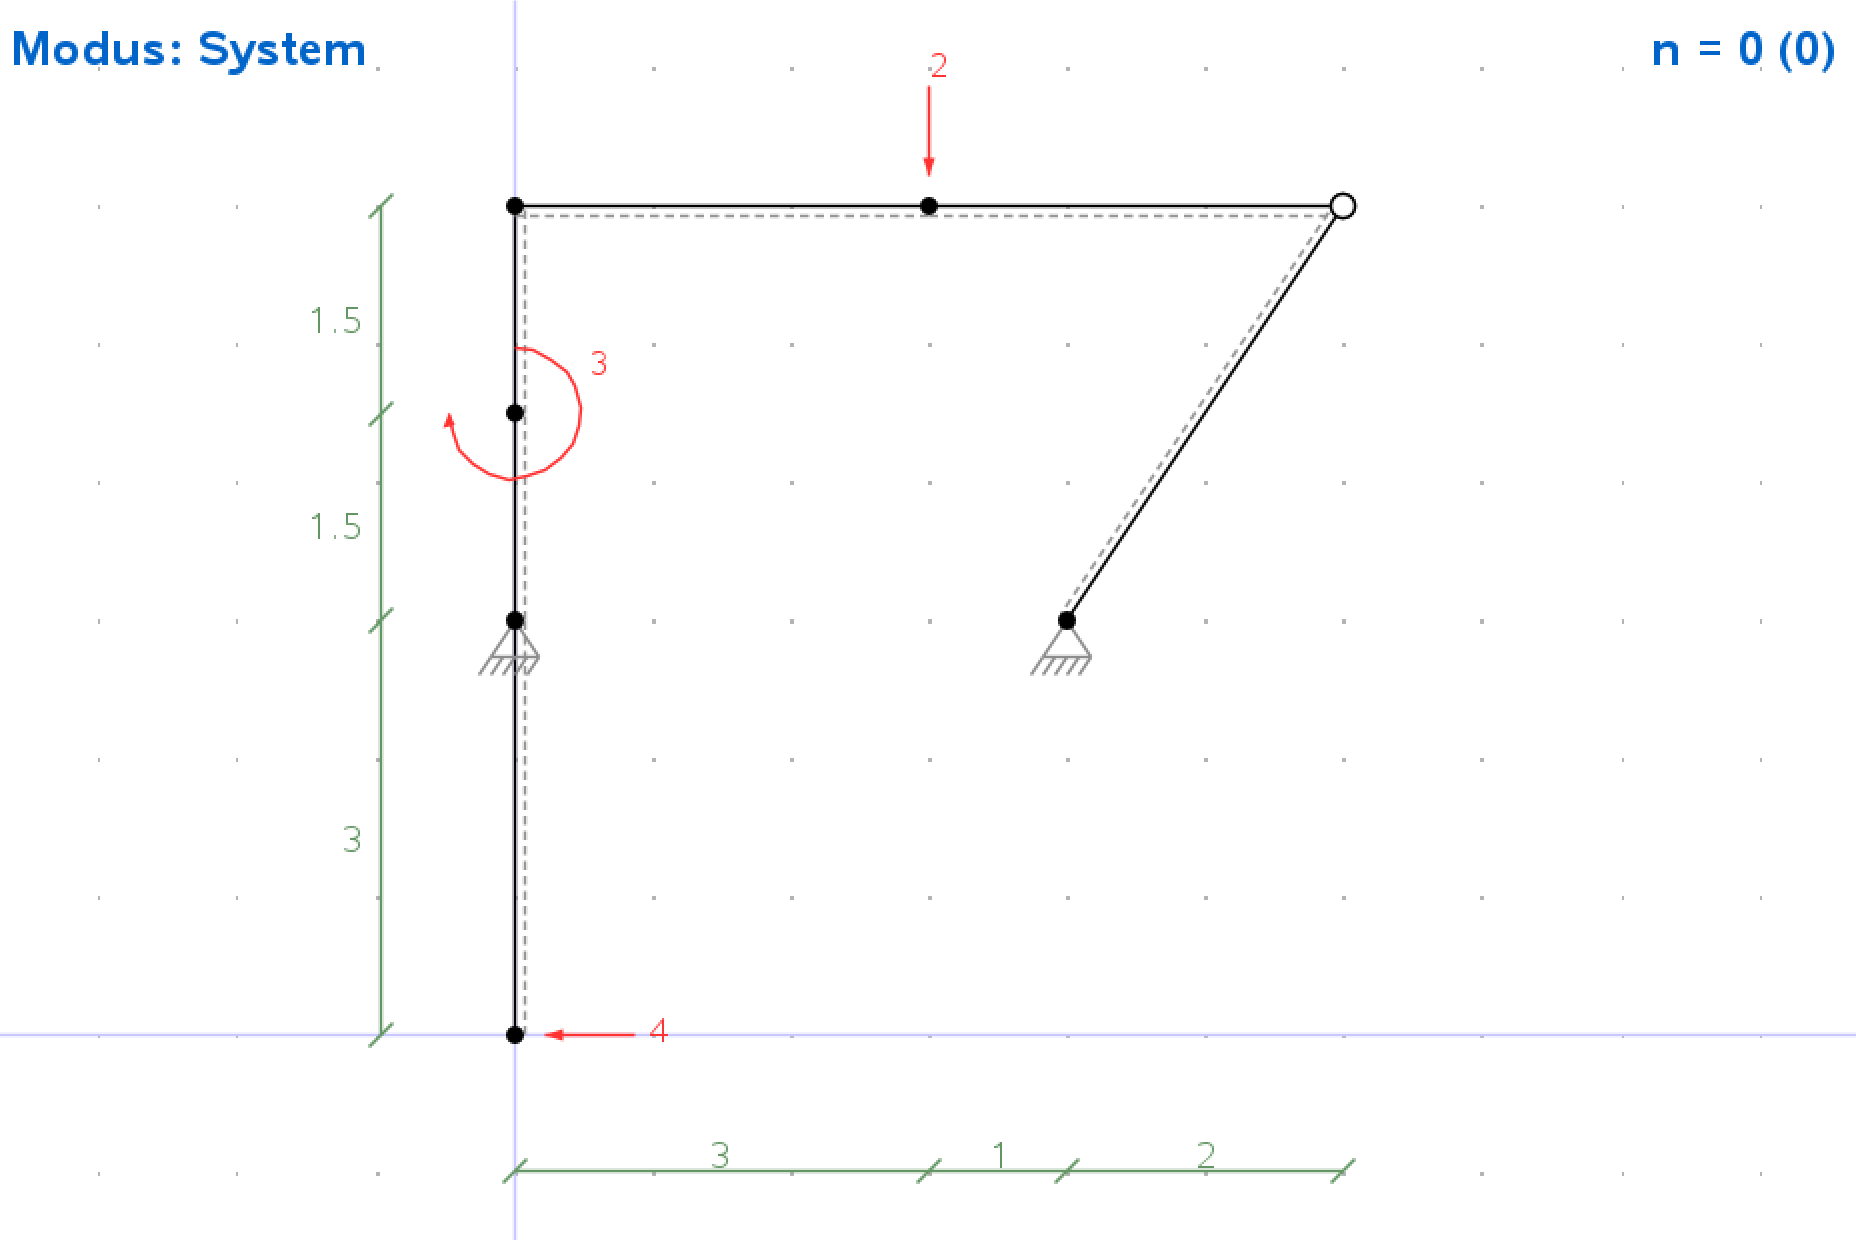
\includegraphics[width=0.5\linewidth]{./fig/TM1/WiSe2122nr3_1.png}
    \caption{TM1 WiSe~21/22, Nr.~3 im Programm}
    \label{fig:TM1WiSe2122Nr3_1}
\end{figure}

\begin{figure}[htbp]
    \centering
    \begin{subfigure}[t]{0.48\textwidth}
        \centering
        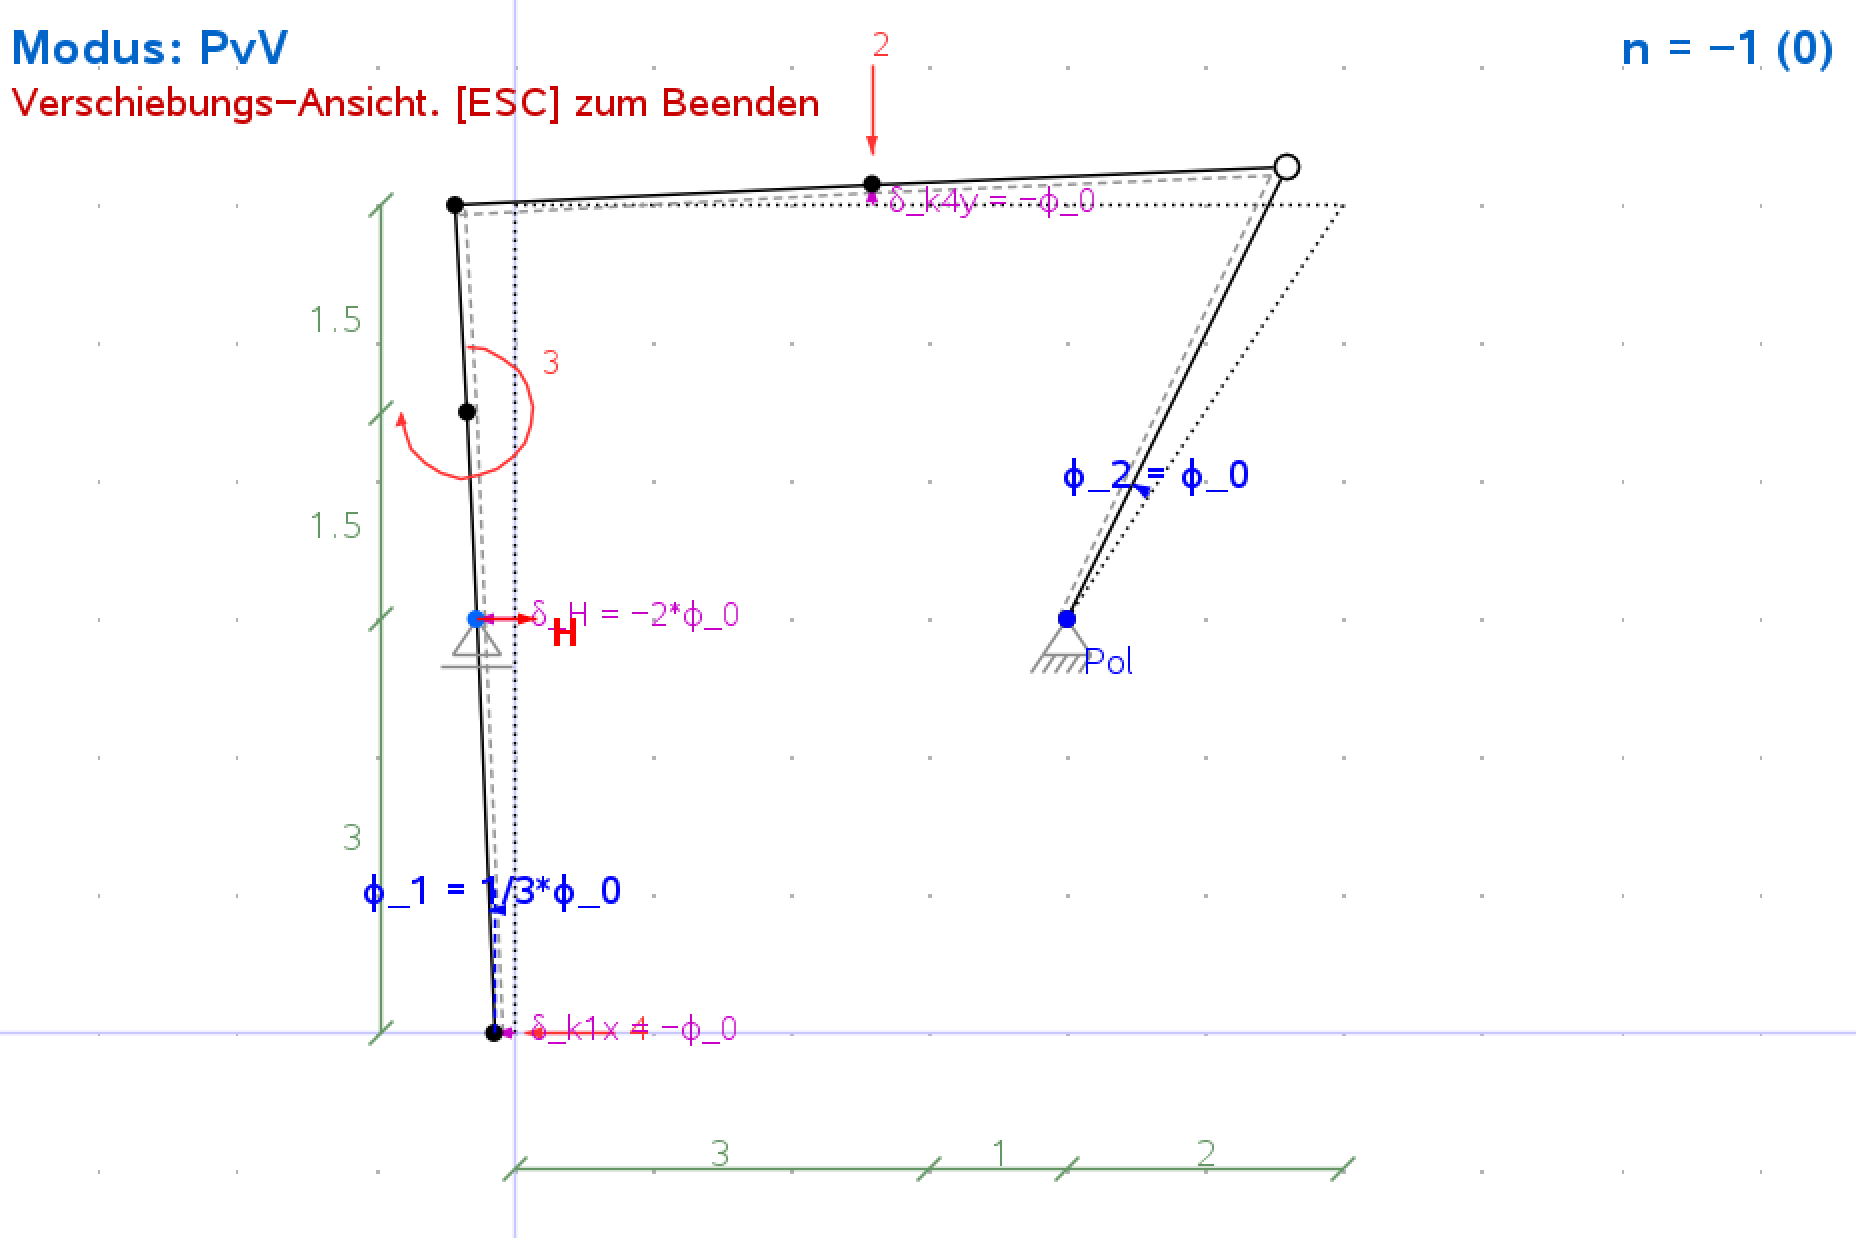
\includegraphics[width=\linewidth]{./fig/TM1/WiSe2122nr3_2.png}
        \caption{Verschiebungsfigur für $A_H$}
    \end{subfigure}
    \hfill
    \begin{subfigure}[t]{0.48\textwidth}
        \centering
        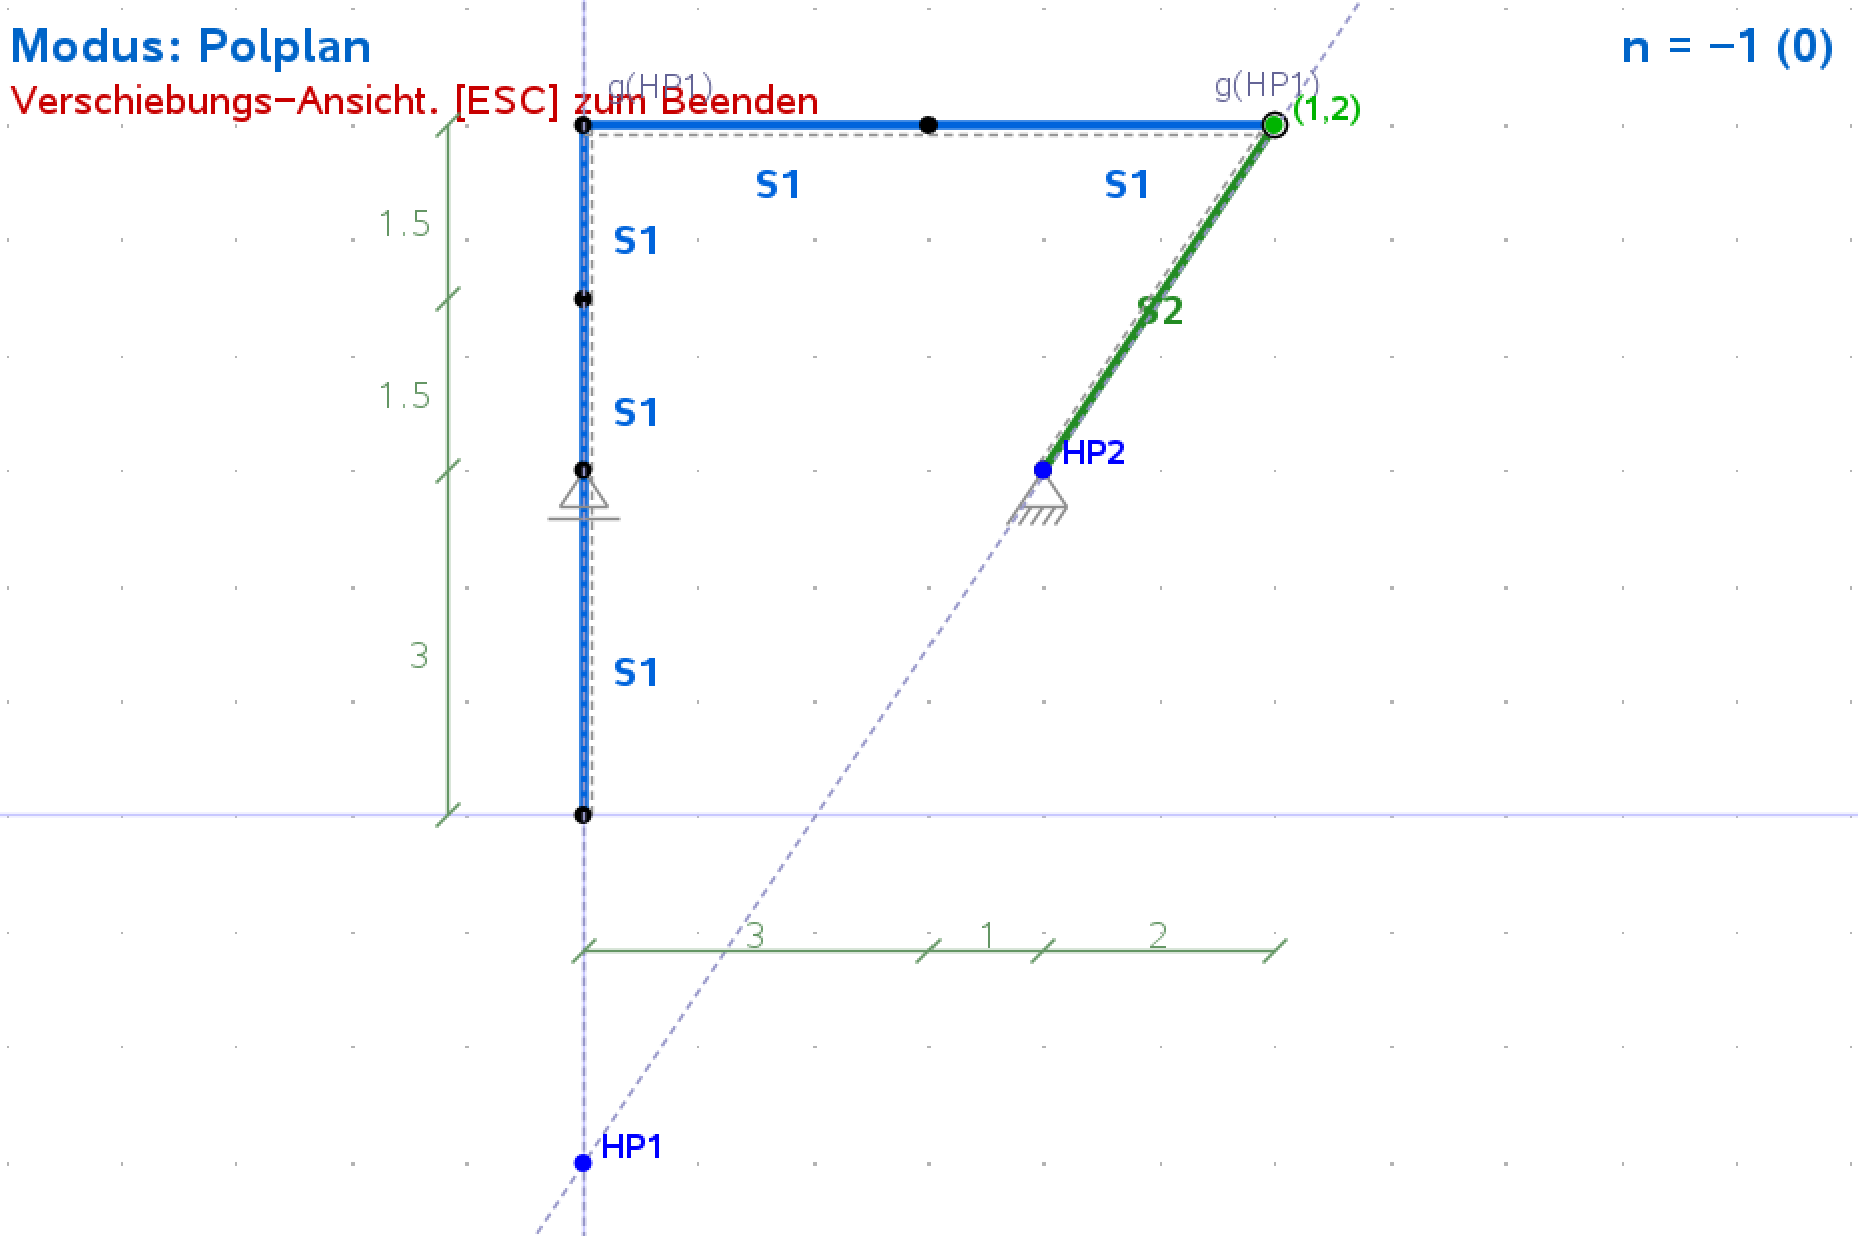
\includegraphics[width=\linewidth]{./fig/TM1/WiSe2122nr3_3.png}
        \caption{Polplan für $A_H$}
    \end{subfigure}
    \caption{WiSe~21/22, Nr.~3: $A_H$}
    \label{fig:TM1WiSe2122Nr3_2}
\end{figure}

\begin{figure}[htbp]
    \centering
    \begin{subfigure}[t]{0.48\textwidth}
        \centering
        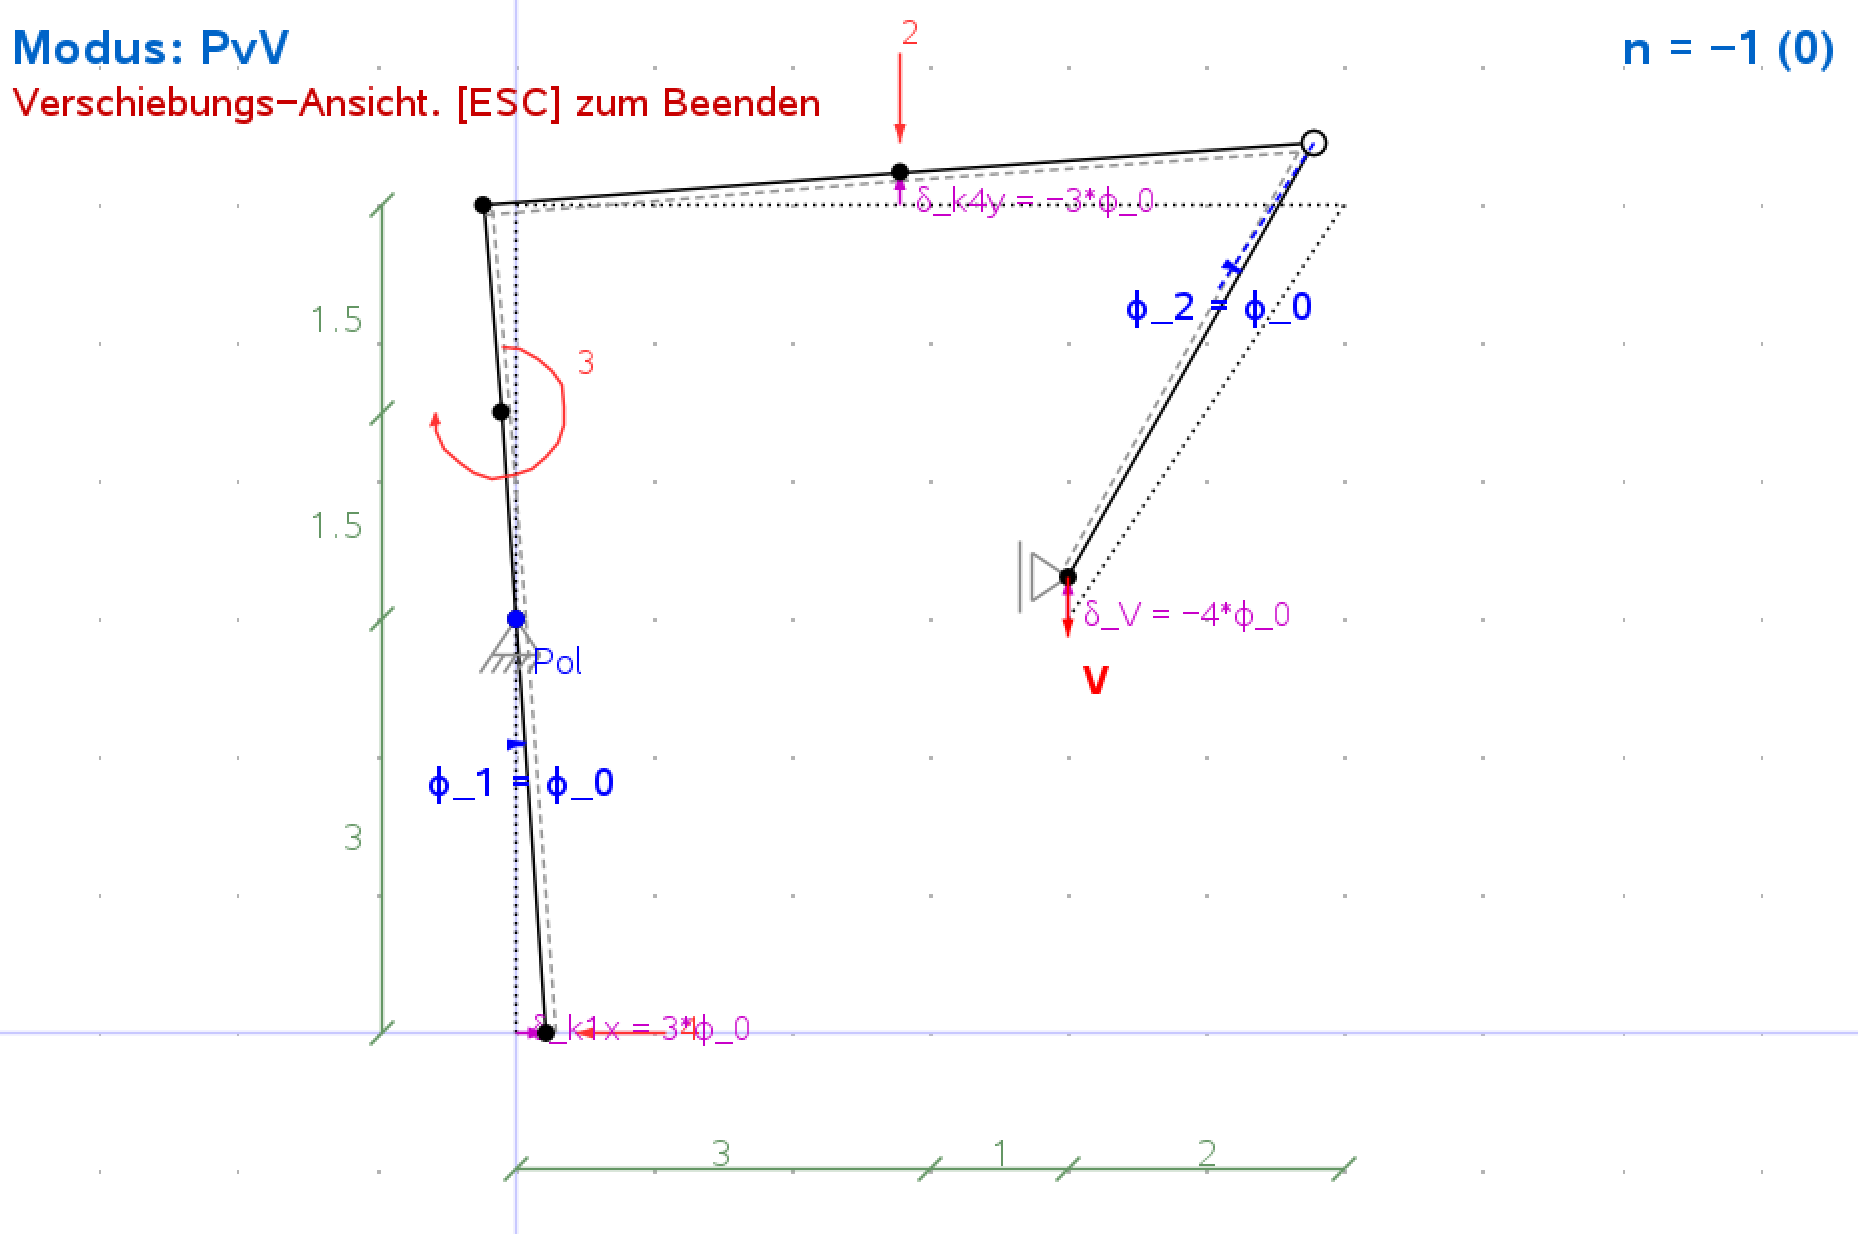
\includegraphics[width=\linewidth]{./fig/TM1/WiSe2122nr3_4.png}
        \caption{Verschiebungsfigur für $B_V$}
    \end{subfigure}
    \hfill
    \begin{subfigure}[t]{0.48\textwidth}
        \centering
        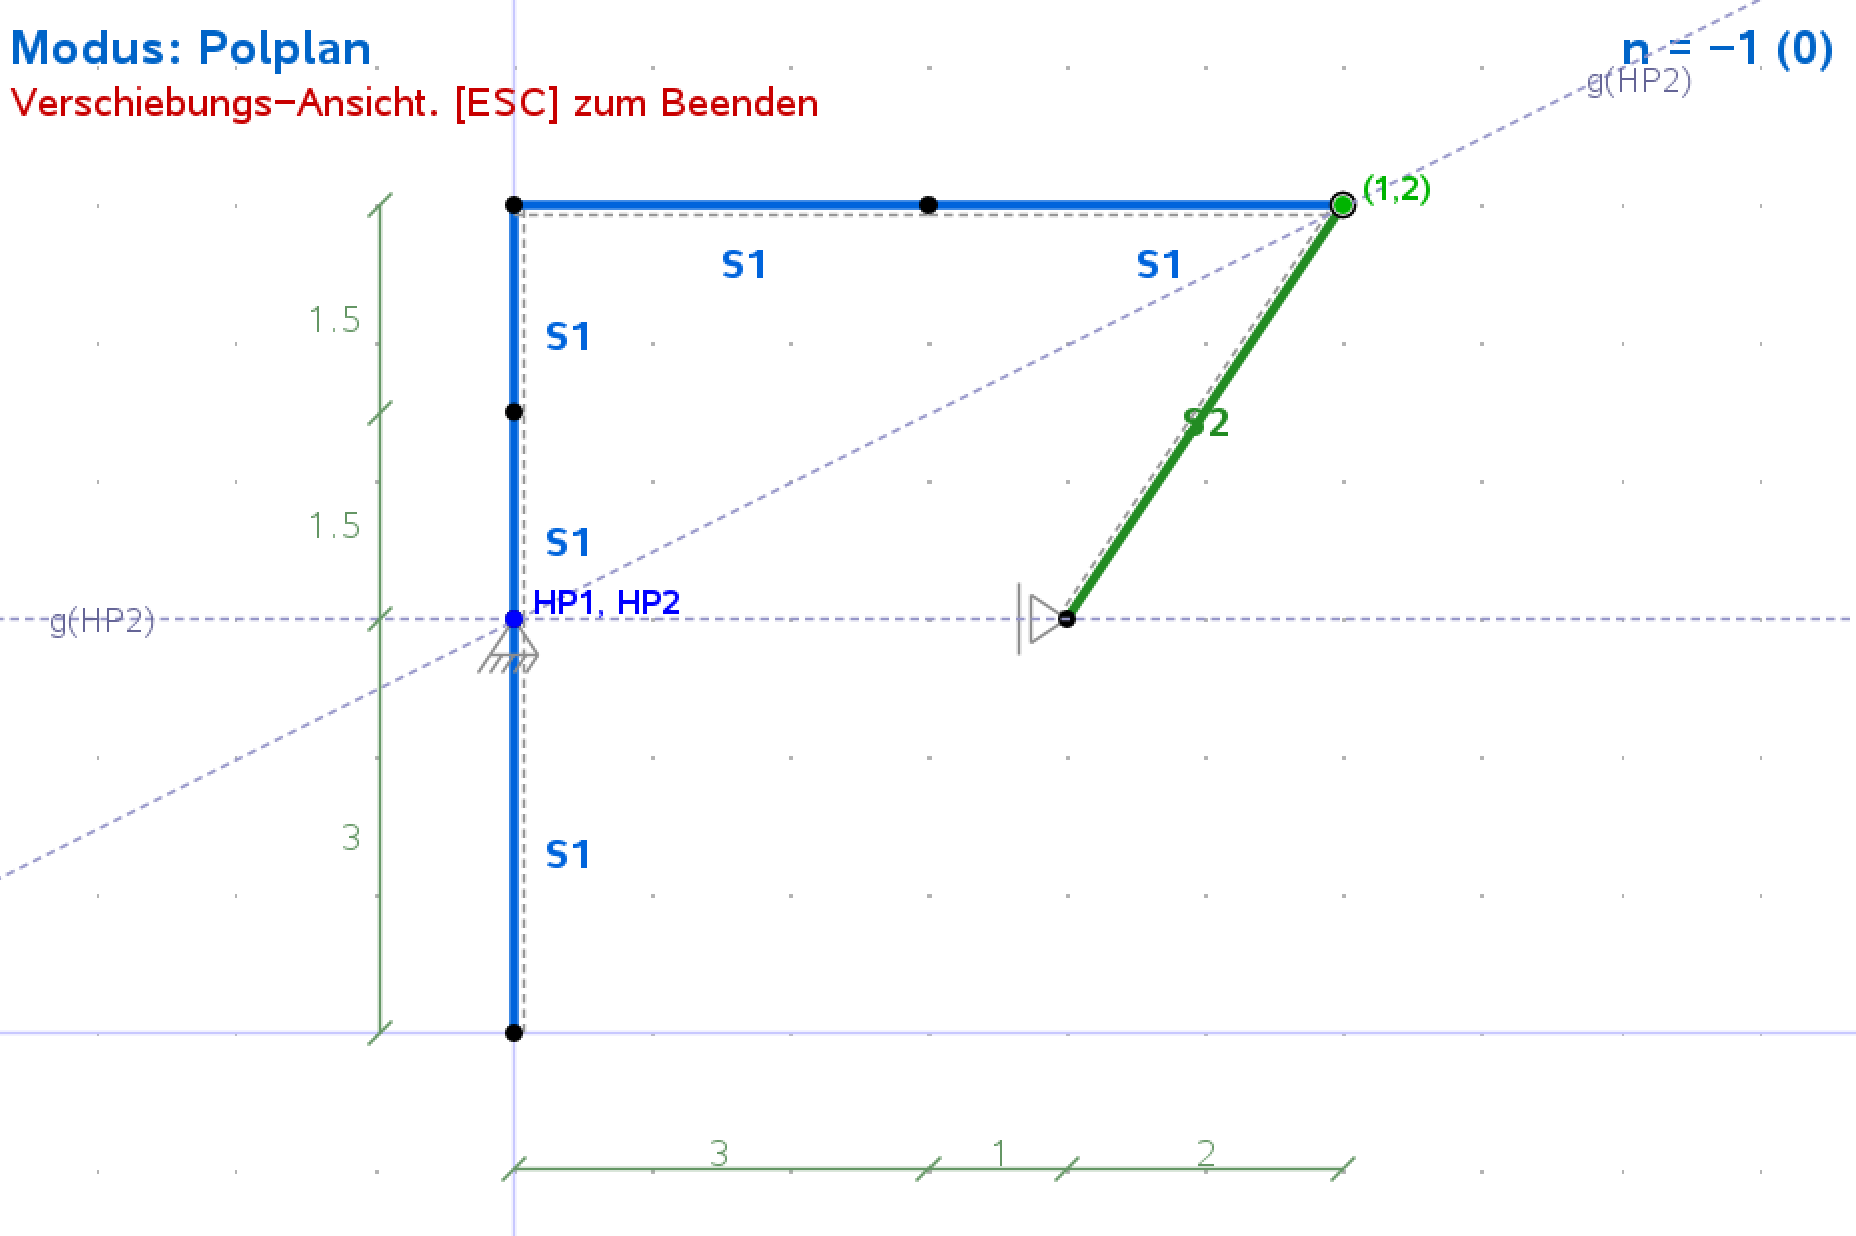
\includegraphics[width=\linewidth]{./fig/TM1/WiSe2122nr3_5.png}
        \caption{Polplan für $B_V$}
    \end{subfigure}
    \caption{WiSe~21/22, Nr.~3: $B_V$}
    \label{fig:TM1WiSe2122Nr3_3}
\end{figure}

Die Zeilen der Matrizen \code{pvv\_kin} und \code{pvv\_pol} (Abb.~\ref{fig:TM1WiSe2122Nr3_4})
sind als Gleichungskette zu lesen. Hier gilt also z.B. $\delta_{k1x}= -3\cdot\varphi_1=-\varphi_0$, oder 
$\delta x_{p12}= -9\cdot\varphi_1=-3\varphi_2$. Mit diesen Gleichungen lässt sich aus \code{w\_eq1} \code{w\_eq2} bauen.
Diese gleichung lässt sich dann entweder von hand oder mit dem Taschenrechner nach der gesuchten Größe auflösen.

\begin{figure}[htbp]
    \centering
    \begin{subfigure}[t]{0.48\textwidth}
        \centering
        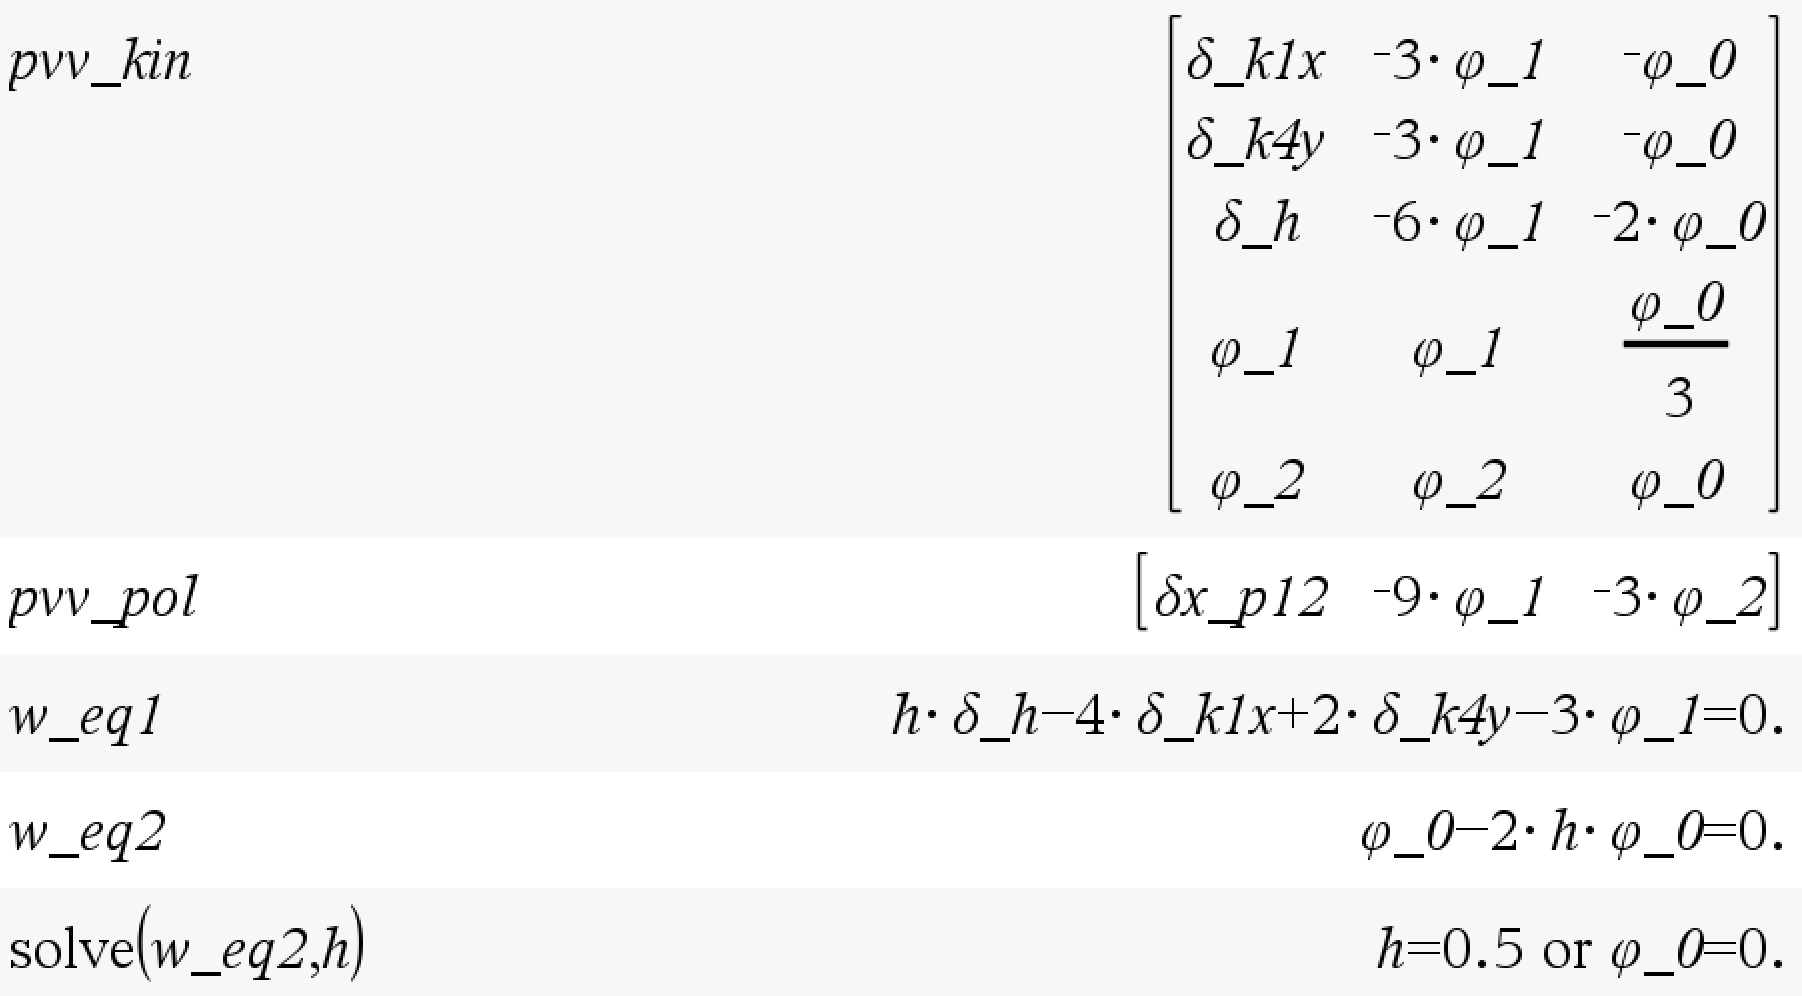
\includegraphics[width=\linewidth]{./fig/TM1/WiSe2122nr3_6.png}
        \caption{Rechnung für $A_H$}
    \end{subfigure}
    \hfill
    \begin{subfigure}[t]{0.48\textwidth}
        \centering
        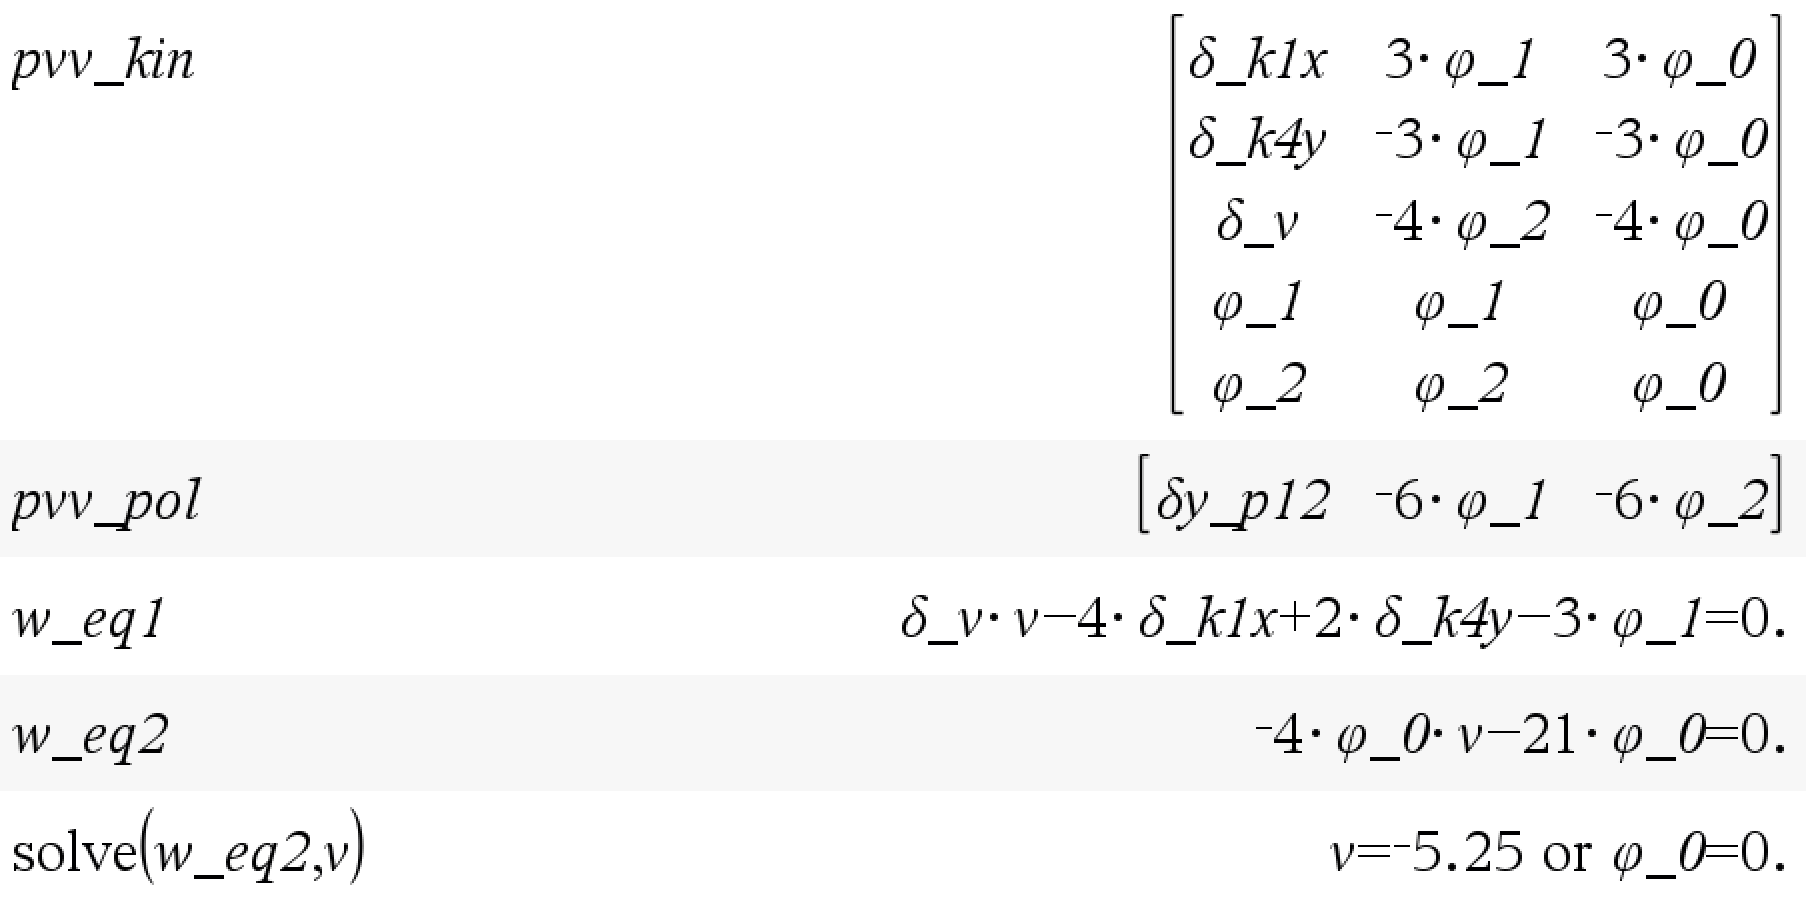
\includegraphics[width=\linewidth]{./fig/TM1/WiSe2122nr3_7.png}
        \caption{Rechnung für $B_V$}
    \end{subfigure}
    \caption{WiSe~21/22, Nr.~3: Ergebnis}
    \label{fig:TM1WiSe2122Nr3_4}
\end{figure}

\subsection{Schnittkräfte Bögen (Nr.~5)}

Mit dem Programm lassen sich die Funktionen für Schnittkraftverläufe von normalen Stäben als auch von Bögen 
ausgeben. Bei bögen ist die Laufvraibale nur nicht mehr die Länge entlang des Stabes sondern der Winkel.
also für diese Aufgabe zweilmal $\varphi \in [0,\frac{\pi}{4}]$ bzw. $\varphi \in [0,90\text{°}]$. Hier ist die Winkel-Einstellung
des Taschenrechenrs wichtig.\\
Hier gilt aber auch wieder, dass das Programm das nicht wirklich so ausrechnet wie man das von Hand machen würde, sondern
es sucht eine schöne Darstellung der Anfangswerte und kombiniert diese dann zur Funktion.

\begin{figure}[htbp]
    \centering
    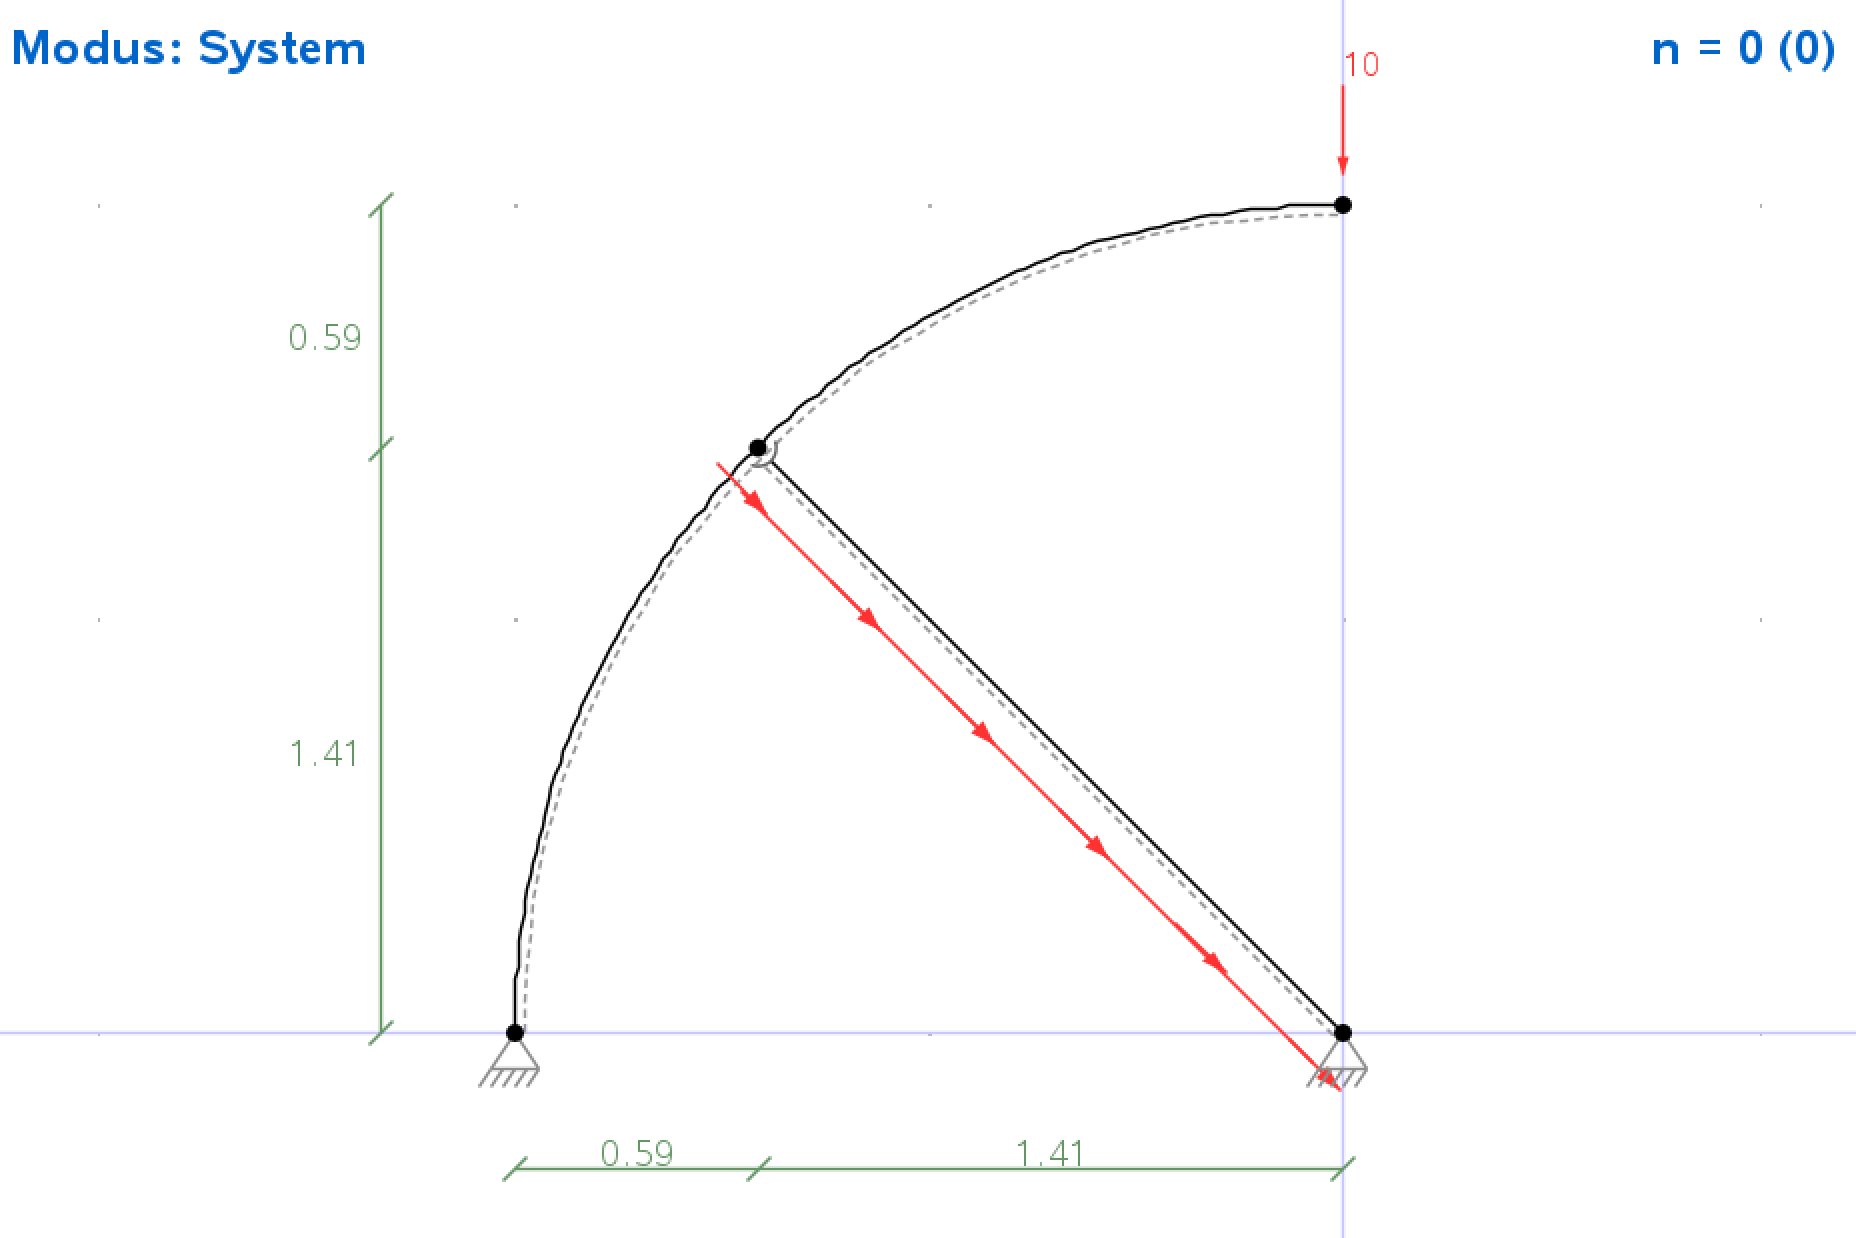
\includegraphics[width=0.5\linewidth]{./fig/TM1/WiSe2122nr5_1.png}
    \caption{TM1 WiSe~21/22, Nr.~5 im Programm}
    \label{fig:TM1WiSe2122Nr5_1}
\end{figure}


\subsection{Fachwerk (Nr.6)}

Vom Prinzip werden Fachwerke genau gleich eingegeben wie normale Systeme, nur das hier die orientierung der gestrichelten Faser
keine Rolle spielt. Es ist jedoch sinnvoll den Fachwerk Modus anzumachen, dann wird die statische Bestimmtheit beim hovern über $n=$ 
auch die Formel für Fachwerke verwendet und alle Knoten werden zu vollgelenken gemacht, auch wenn der Modus erst nach dem 
zeichnen des Systems angemacht wird.  


\begin{figure}[htbp]
    \centering
    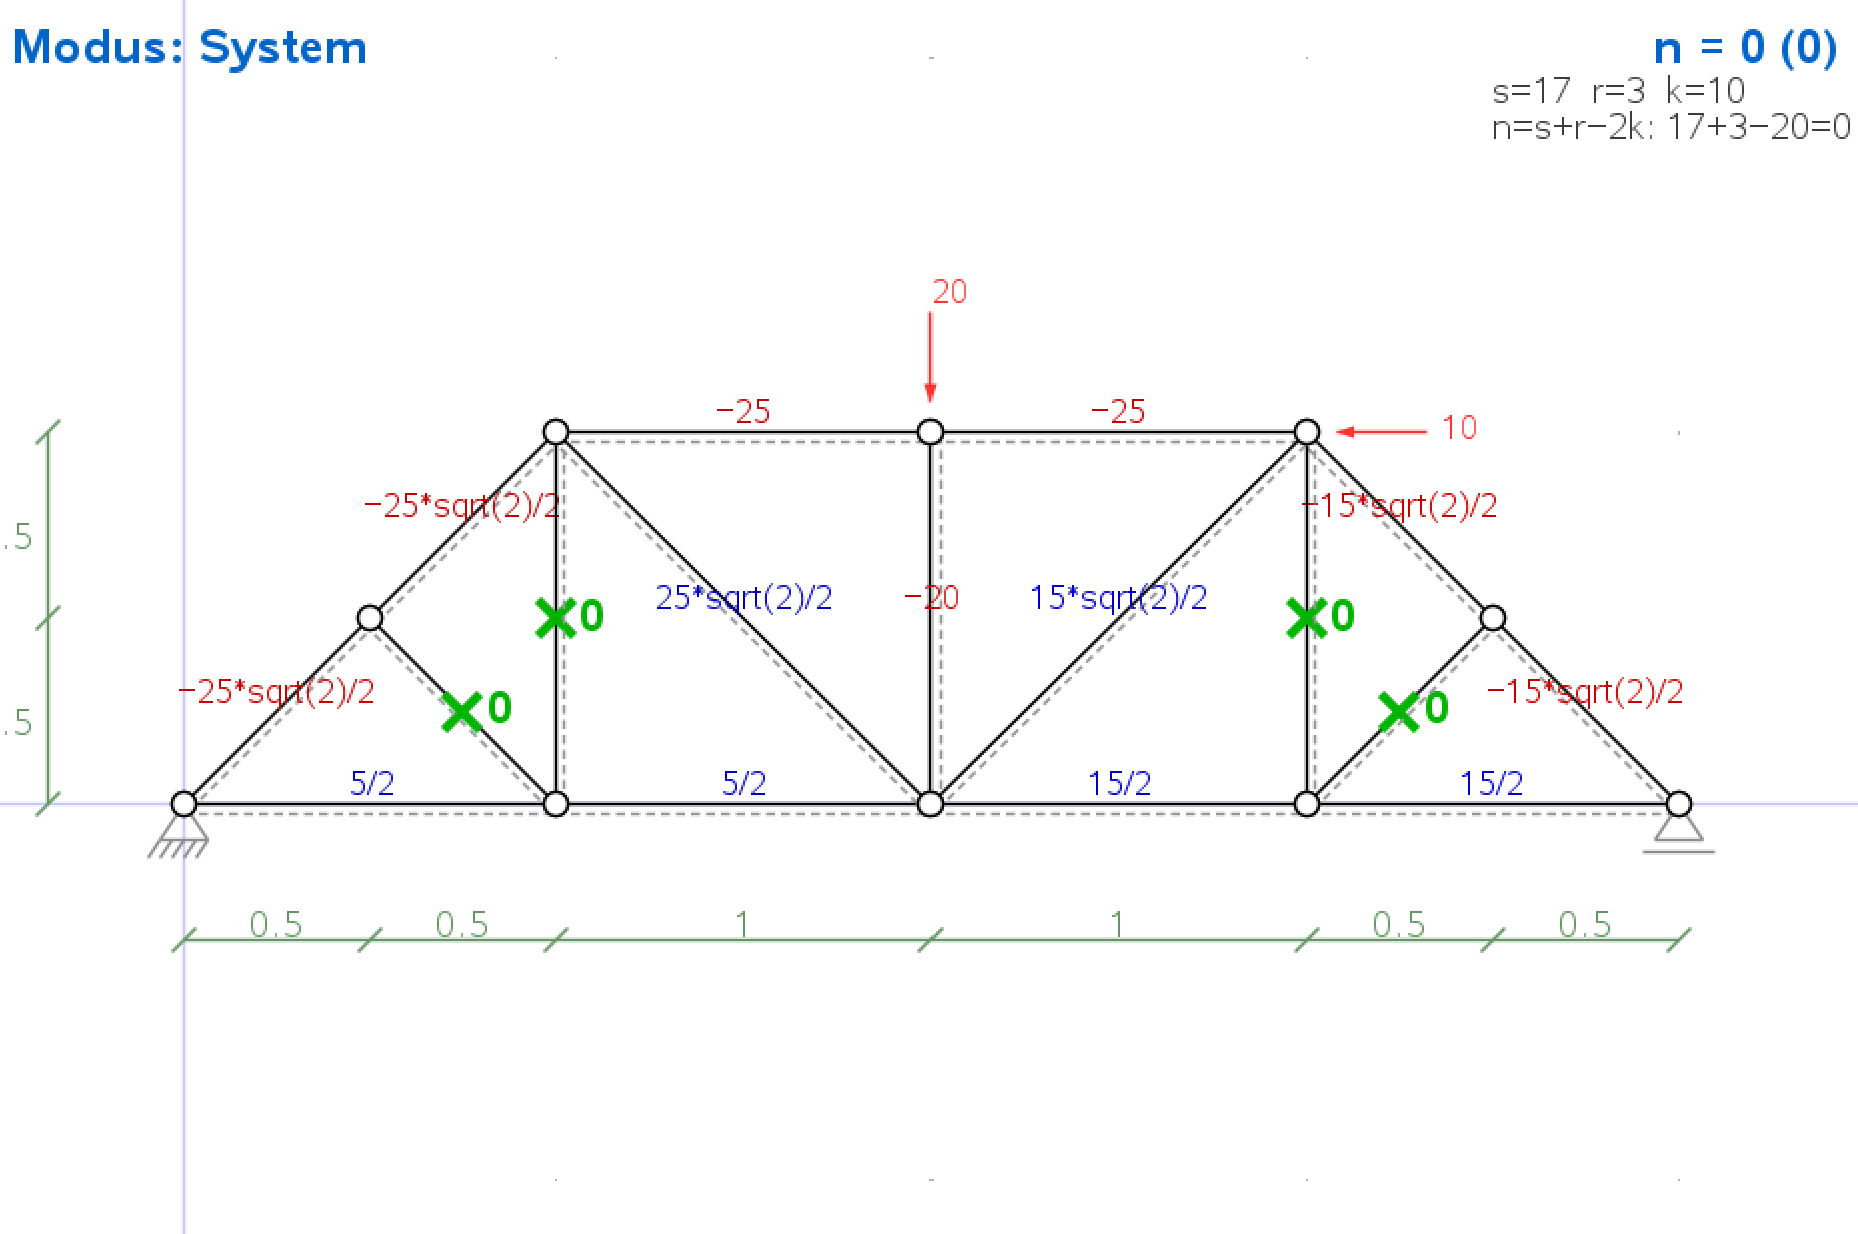
\includegraphics[width=0.5\linewidth]{./fig/TM1/WiSe2122nr6_1.png}
    \caption{TM1 WiSe~21/22, Nr.~6 im Programm}
    \label{fig:TM1WiSe2122Nr6_1}
\end{figure}

Die Stabe in Abb.~\ref{fig:TM1WiSe2122Nr6_1} die ein grünes Kreuz haben sind die ohne Rechnung erkennbaren Nullstäbe
Falls nach der Berechnung stäbkkräfte mit einer grünen Null beschriftet werdsen, aber dort kein Kreuz ist, ist das zwar ein 
Nullstab der aber nicht direkt aus den Regeln erkennbar ist. Für Afgaben bei denen nach Nullstäben gefragt wird, also nur 
die durchgekreuzten Stäbe angeben

\begin{figure}[htbp]
    \centering
    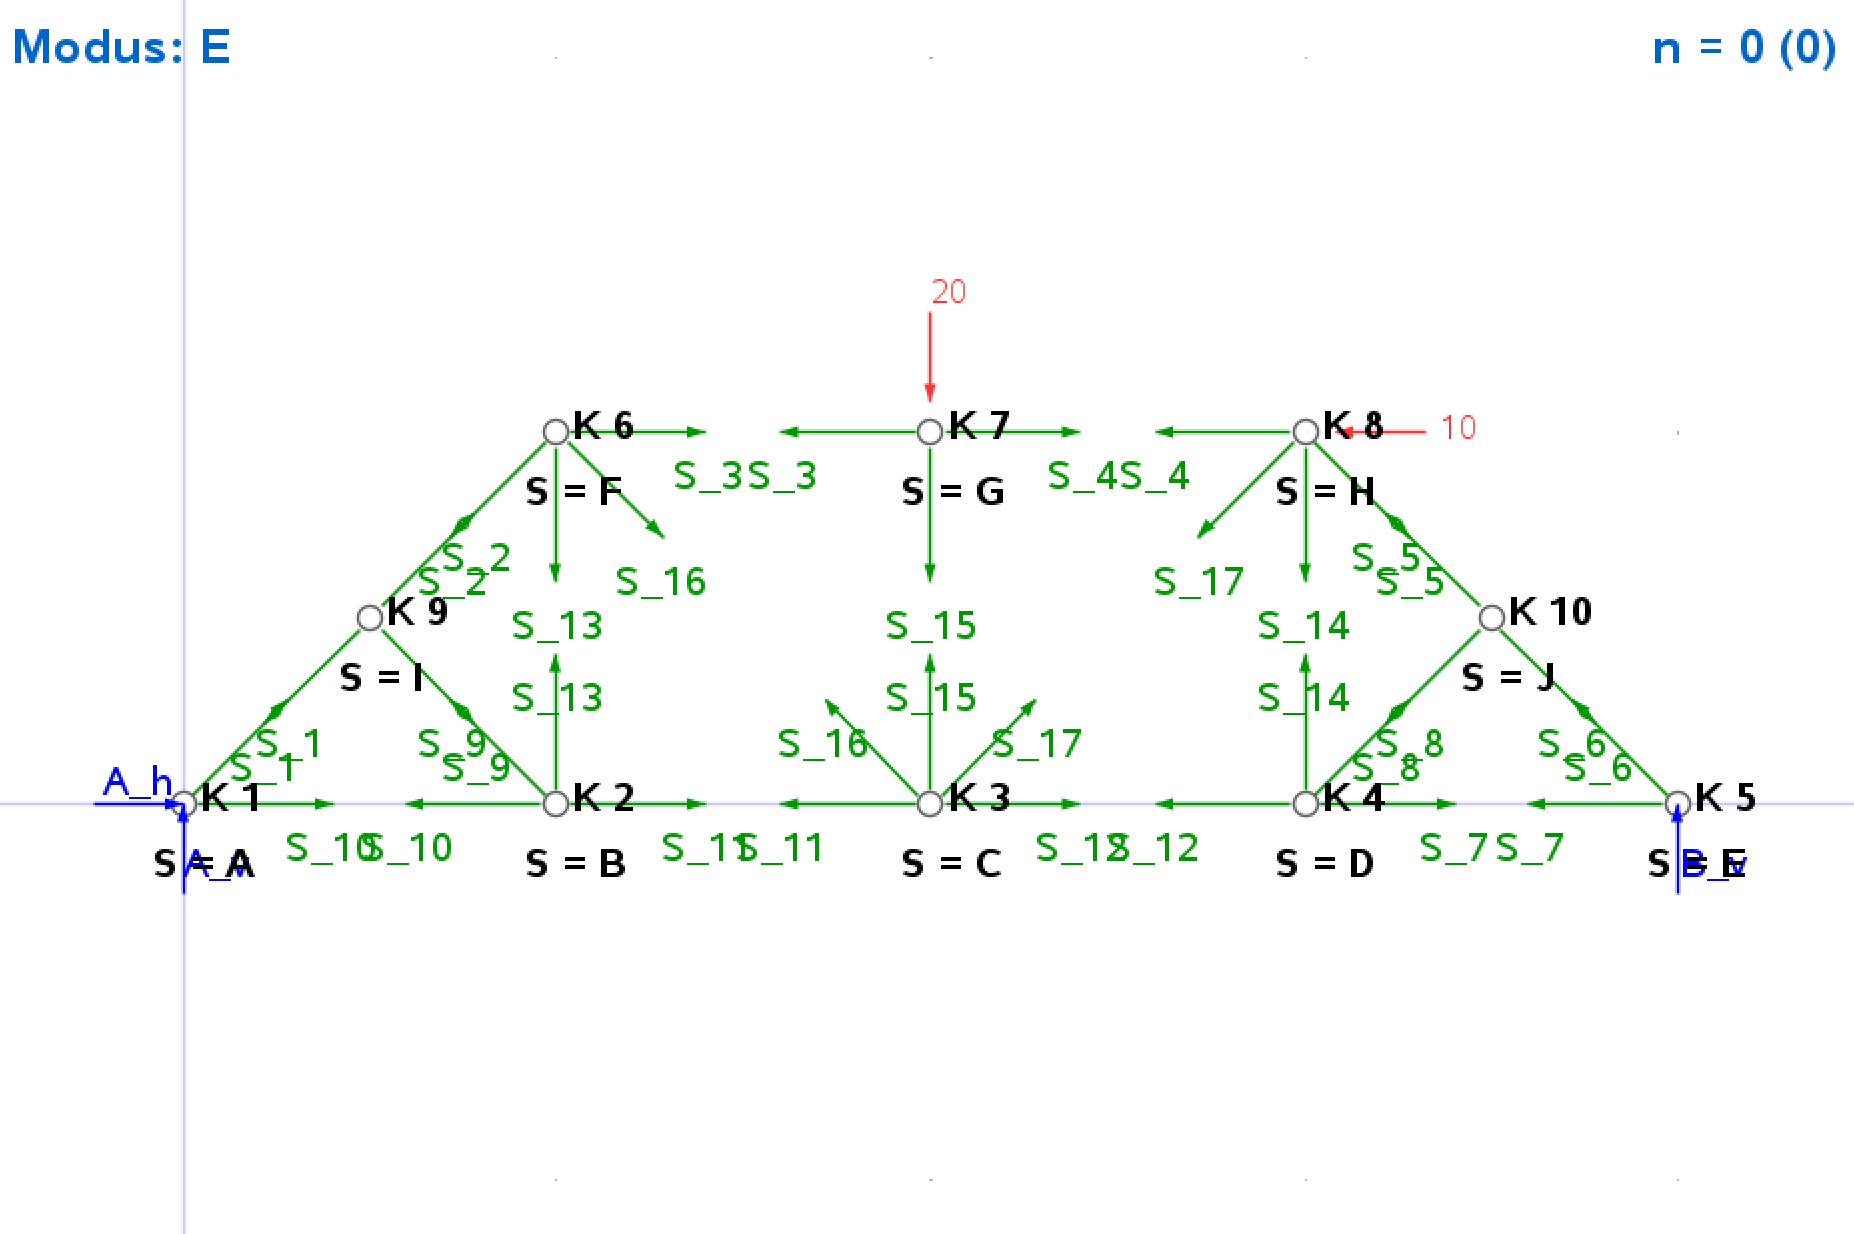
\includegraphics[width=0.5\linewidth]{./fig/TM1/WiSe2122nr6_2.png}
    \caption{TM1 WiSe~21/22 Freischnitt}
    \label{fig:TM1WiSe2122Nr6_2}
\end{figure}

Für die Verwendung der beiden Seiten des E-Modus muss darauf geachtet werden, dass entweder die Stäbe in der
gleichen Reihenfolge wie in der Aufgabe gezeichnet werden oder die Bennenung hinterher angepasst wird. Macht ihr das nicht
ist z.B. Stab 13 aus eurer Rechnung nicht Stab 13 aus der Aufgabe\\
Gleiches gilt natürlich auch für die Verwendung des LGS-Exports. Hier wird (Falls der Fachwerk Modus an ist) 
das Knotenschnittverfahren verwendet. Die Benennung im LGS ist die gleiche wie auf der zweiten Seite des E-Modus.





\section{TM2}

\subsection{Biegelinie (TM2 WiSe~21/22, Nr.~7)} \label{ex:Biegelinienaufgabe}

In dieser Aufgabe ist ein \emph{interessantes} KOS vorgegeben: Soll es ein Rechtssystem sein,
zeigt die $y$-Achse hier in die Zeichenebene hinein und nicht, wie sonst üblich, aus ihr heraus.

Rechnet ihr von Hand über die DGL $EI\,w'''' = q$ mit allen Rand- und Übergangsbedingungen (so
geht man bei statisch unbestimmten Systemen meist vor, und so rechnet auch \code{wneu}), gibt es
hier nichts weiter zu beachten. Bei einem statisch bestimmten System lohnt es sich dagegen, zuerst
die Momentenlinie zu berechnen und dann $EI\,w'' = -M$ zu integrieren. Dafür braucht ihr die
gestrichelte Faser. Die Regel aus Abschnitt~\ref{sec:Eingabe_Stäbe}, dass sie immer auf der Seite
liegt, in die die $z$- bzw.\ $w$-Achse zeigt, gilt auch hier. Alternativ könnt ihr euch überlegen,
auf welcher Seite ein positives Schnittmoment $M_y$ (Drehsinn nach der Rechte-Hand-Regel um die
$y$-Achse) Zug erzeugt, dort liegt die gestrichelte Faser. Das finde ich aber umständlicher.

Im Programm müsst ihr solche Systeme etwas anders eingeben, denn dort zeigt die $y$-Achse immer
aus der Zeichenebene heraus. Zeichnet ihr das System genau wie in der Aufgabe und setzt die
gestrichelte Faser nach der Regel oben, läuft die $x$-Koordinate im Programm in die andere Richtung
als in der Aufgabe. Um das zu umgehen, zeichnet ihr Systeme, bei denen die $y$-Achse in die
Zeichenebene hineinzeigt, spiegelverkehrt (Abb.~\ref{fig:Biegelinienaufgabe}). Ich habe die
Aufgabe im symbolischen Modus gerechnet, deshalb stehen in den Ergebnissen $q$ und $l$.

\begin{figure}[htbp]
    \centering
    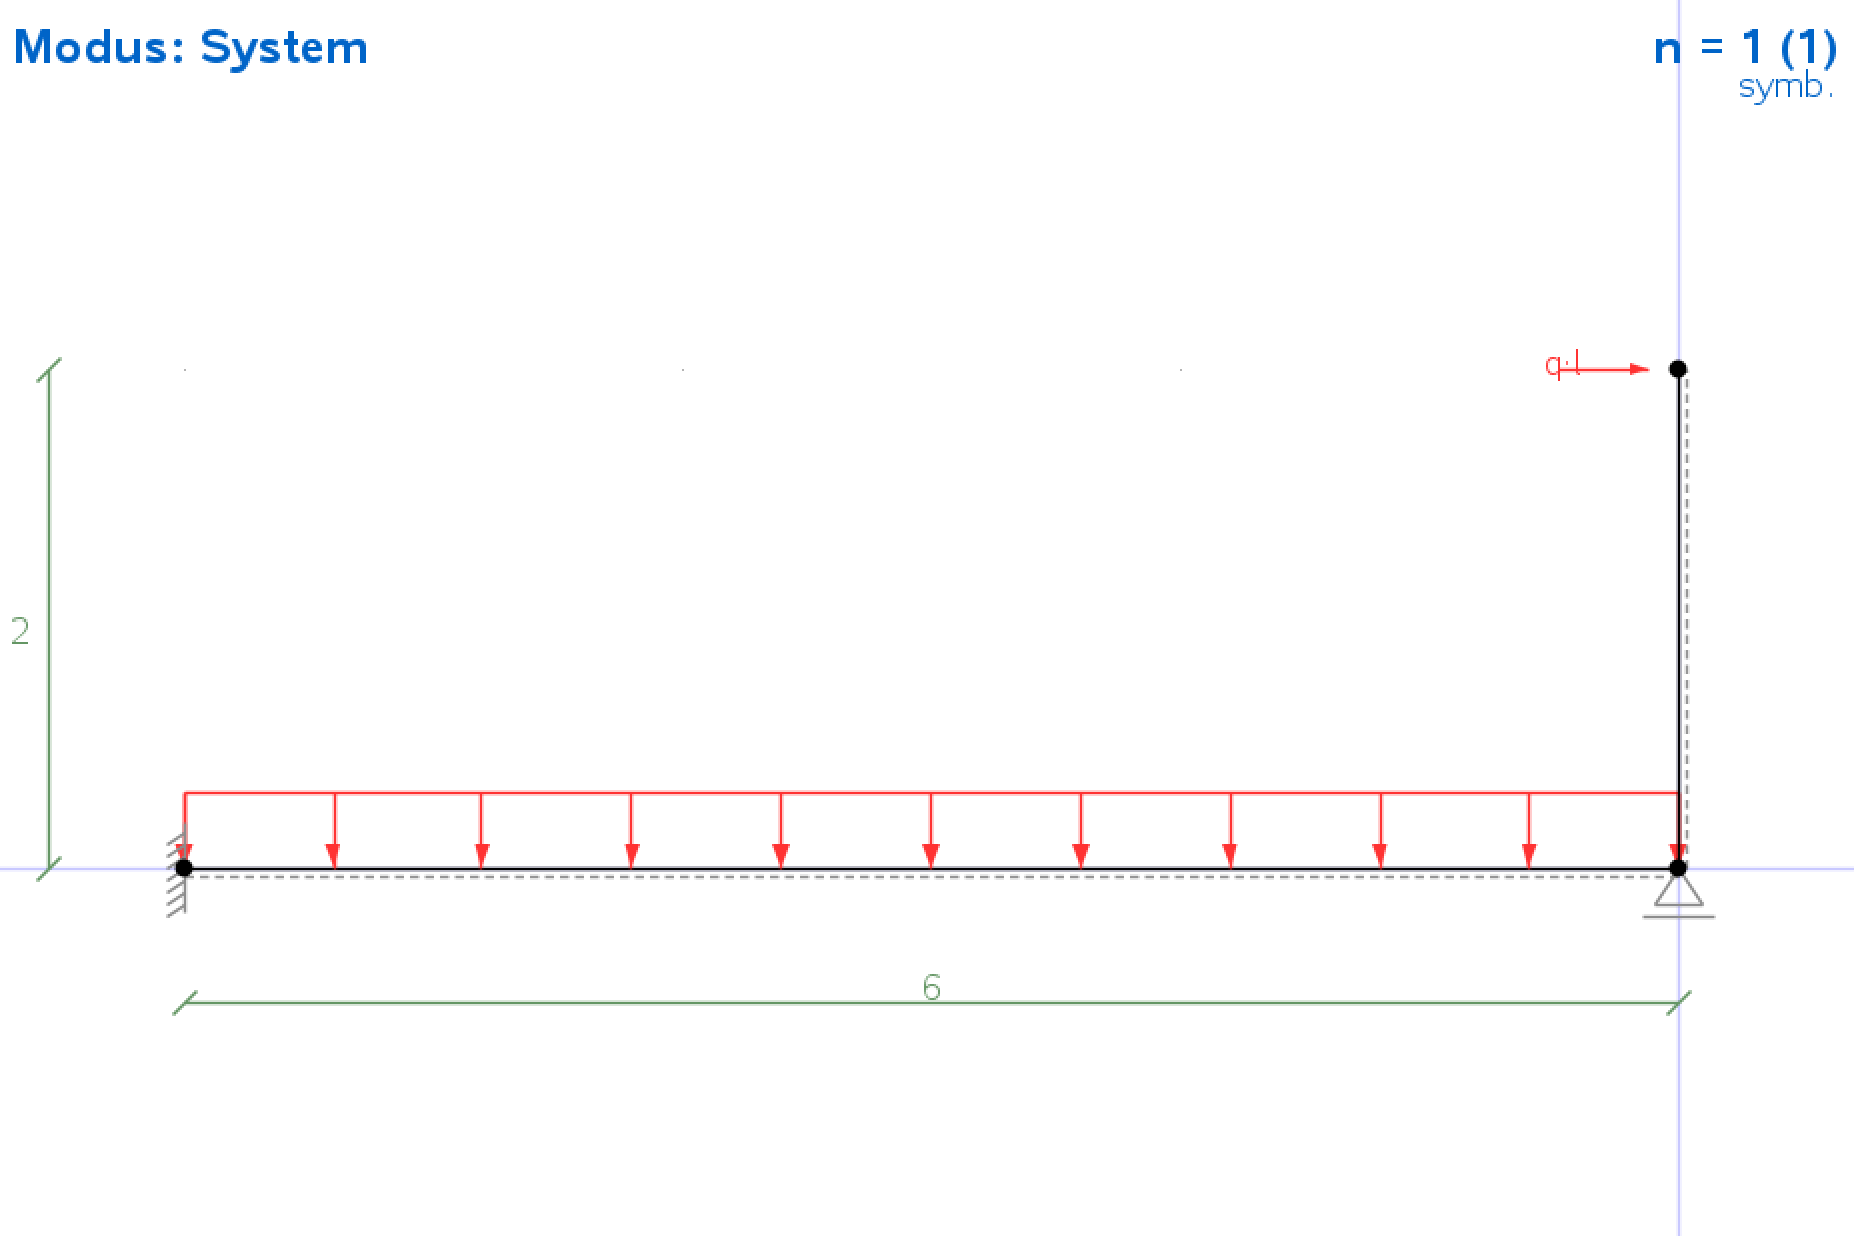
\includegraphics[width=0.5\linewidth]{./fig/TM2/WiSe2122nr7_1.png}
    \caption{TM2 WiSe~21/22, Nr.~7 im Programm, spiegelverkehrt gezeichnet}
    \label{fig:Biegelinienaufgabe}
\end{figure}

Das liefert die Ergebnisse in Abb.~\ref{fig:BiegelinienaufgabeBiegelinie}. Hier geben beide
Methoden dasselbe Ergebnis. Das sollte natürlich so sein, ist aber nicht immer so: Manchmal weicht
die WGV/FEM-Lösung \code{v\_EI\_stab1(x)} (im Rechner klein geschrieben) minimal von der exakten
Lösung \code{wneu1(x)} ab. Weil das Programm die Brüche aus den Zahlen der FEM-Lösung
\emph{errät} (Abschnitt~\ref{sec:mathe-symbolisch}), kann daraus eine ganz anders aussehende
Biegelinie werden. Die Methode über die WGV/FEM-Lösung gibt es trotzdem, vor allem weil ich sie
zuerst programmiert habe (daher wohl auch der Name \code{wneu} der anderen Funktion), und weil sie
bei sehr großen Systemen deutlich schneller sein kann.

\begin{figure}[htbp]
    \centering
    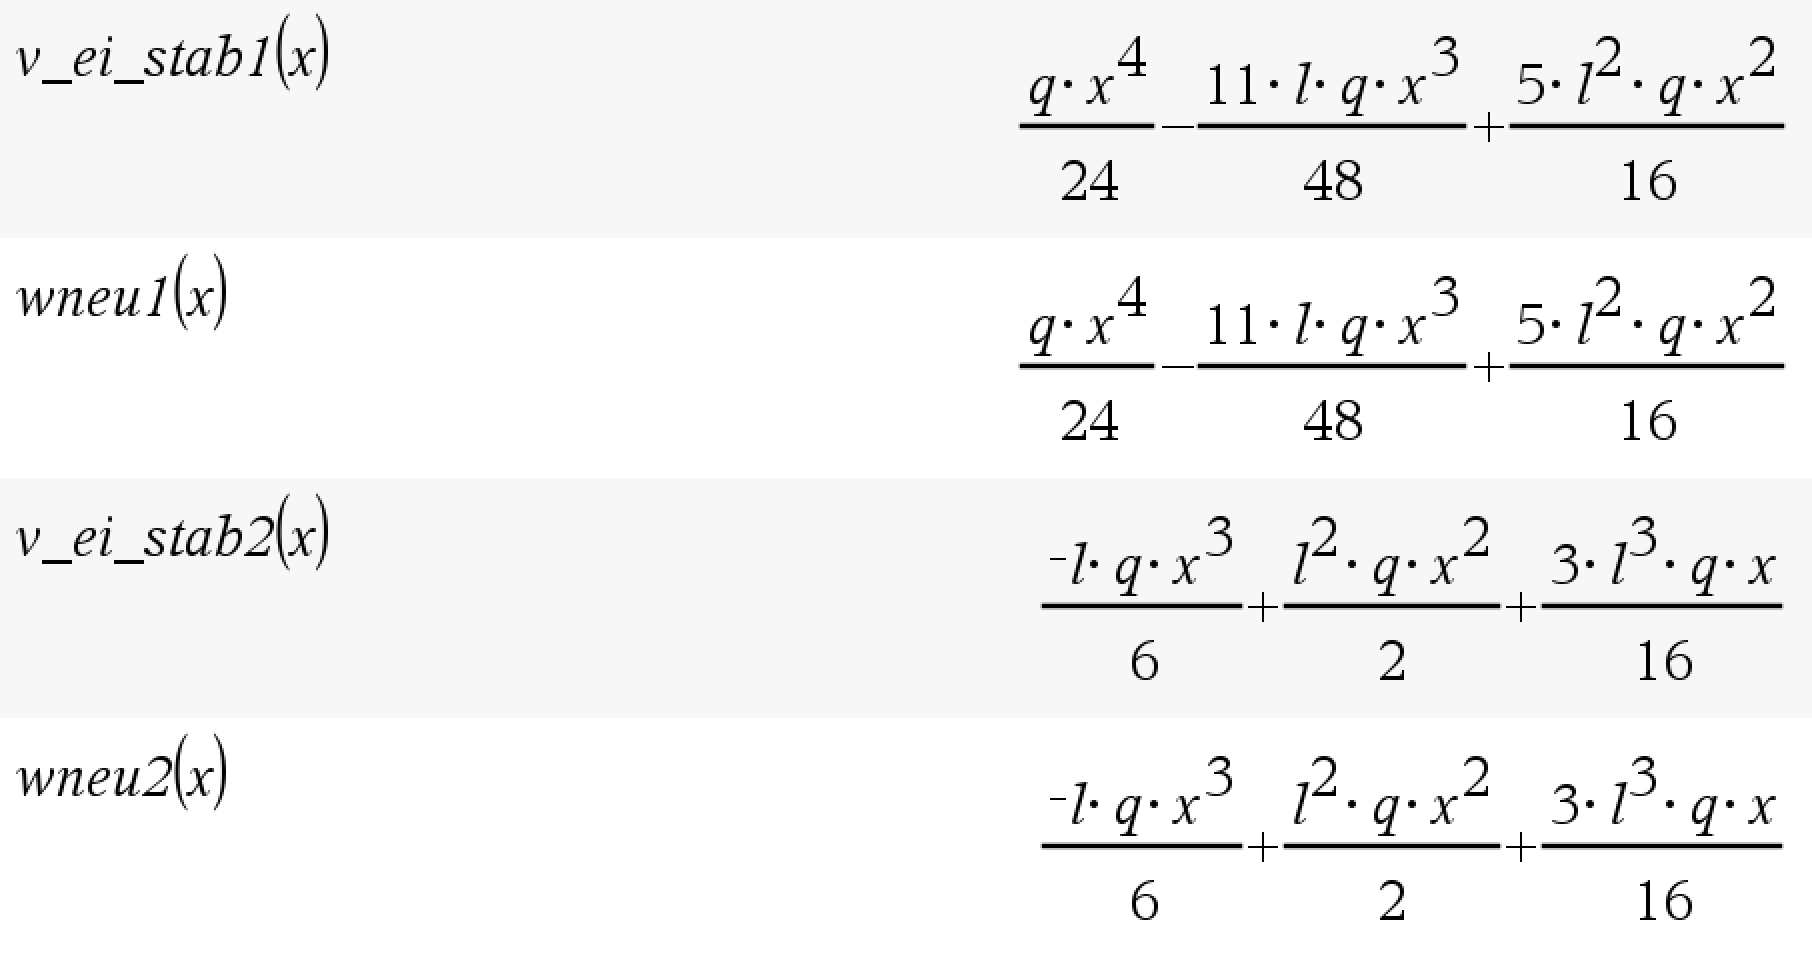
\includegraphics[width=0.5\linewidth]{./fig/TM2/WiSe2122nr7_2.png}
    \caption{TM2 WiSe~21/22, Nr.~7: \code{v\_EI\_stab} und \code{wneu} im Vergleich}
    \label{fig:BiegelinienaufgabeBiegelinie}
\end{figure}

Weil die Stäbe dehnsteif sind, kann das Programm hier sogar die Randbedingungen für Biegelinie und
Längslinie getrennt angeben (Abb.~\ref{fig:BiegelinienaufgabeRandbed}): Die Bedingungen im oberen
Block reichen für die Biegelinie allein, die im unteren kommen nur für die Längslinie dazu. Das geht
nicht immer. Sind die Stäbe dehnbar, hängt die Biegelinie über die Rahmenecken auch von den
Längsverformungen ab, und das Programm gibt alle Bedingungen zusammen aus
(Abschnitt~\ref{sec:randlgs}).

\begin{figure}[htbp]
    \centering
    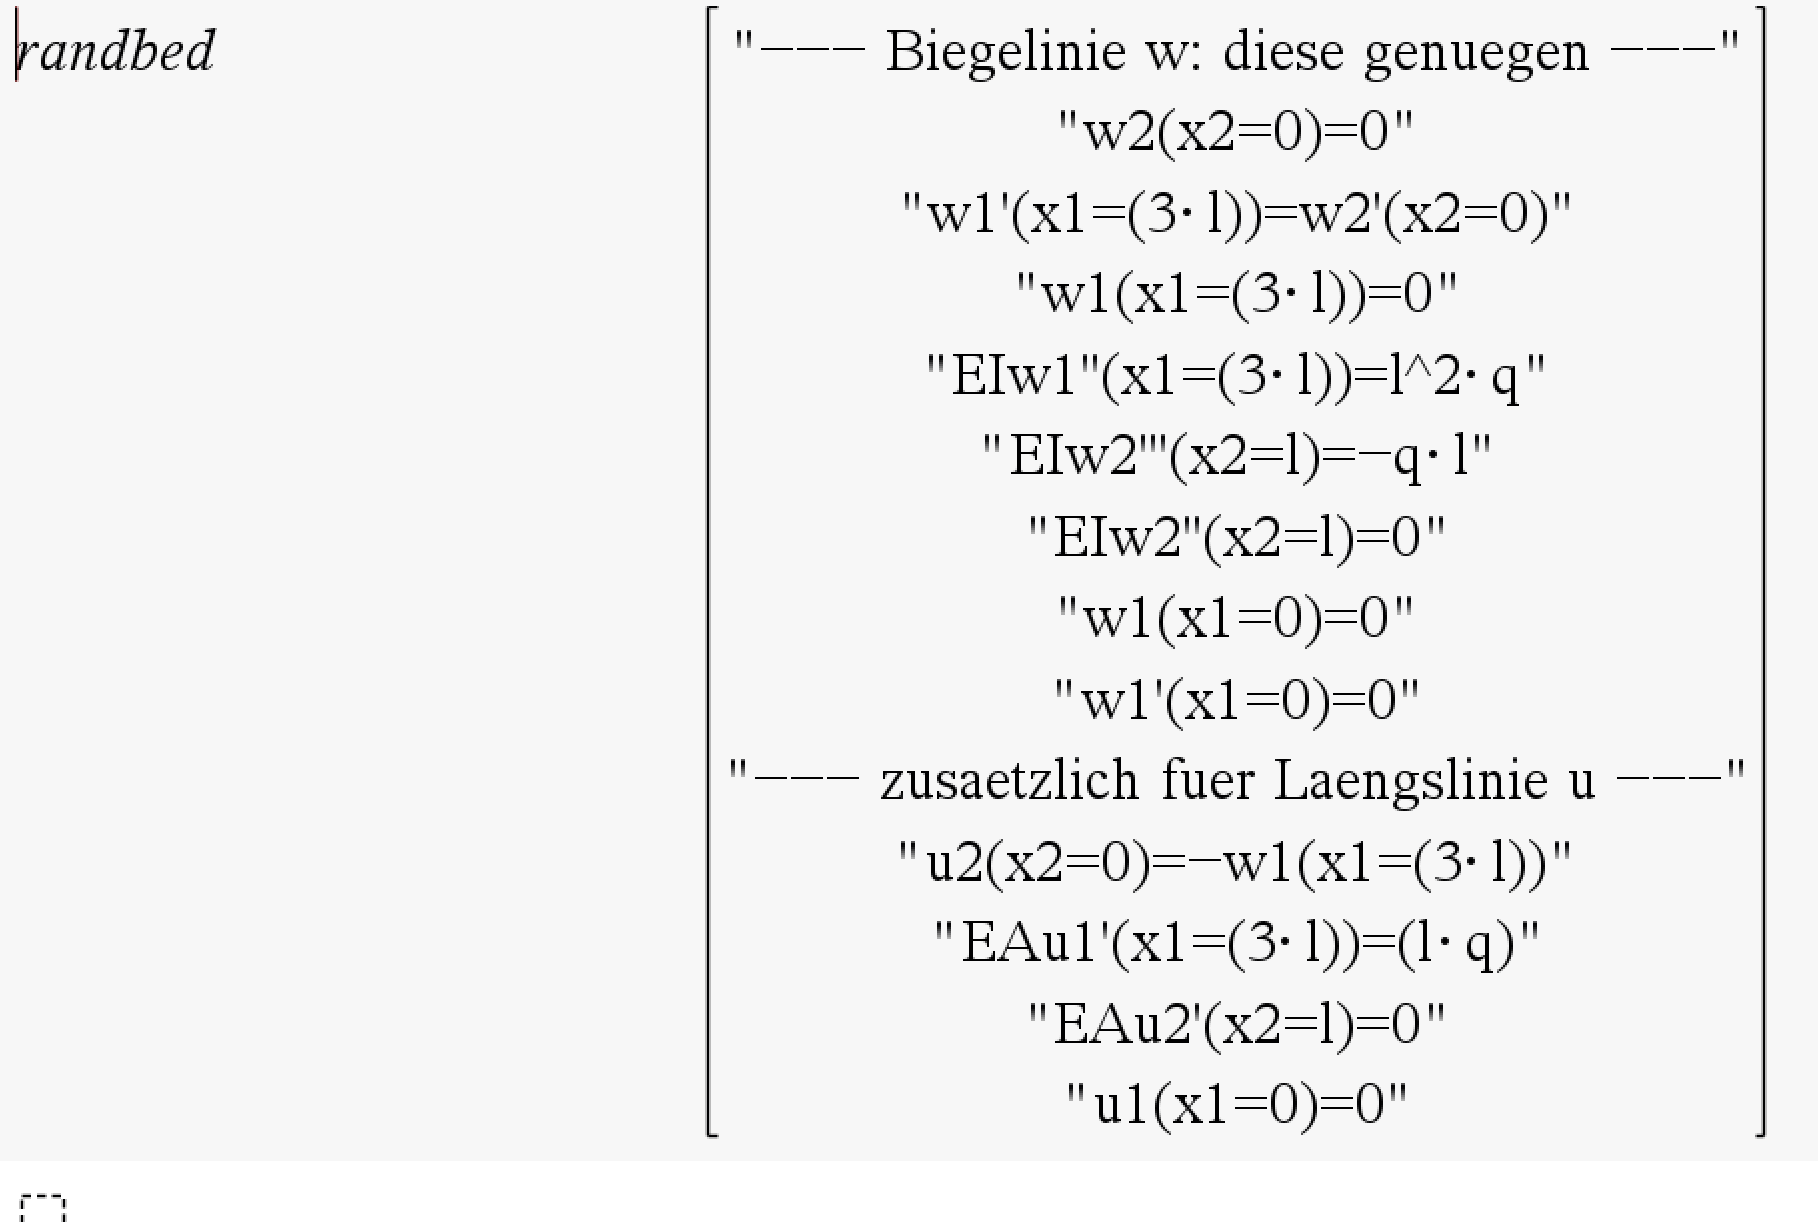
\includegraphics[width=0.5\linewidth]{./fig/TM2/WiSe2122nr7_3.png}
    \caption{Randbedingungen \code{randbed} für TM2 WiSe~21/22, Nr.~7}
    \label{fig:BiegelinienaufgabeRandbed}
\end{figure}



\subsection{Verschiebungsaufgaben (TM2 WiSe~20/21 Nr.~4)} \label{ex:Temperaturaufgabe}

Aufgaben wie diese lassen sich mit der richtigen Eingabe auch direkt im Programm lösen. Wie diese Aufagbe im
Programm aussieht ist in Abb.~\ref{fig:verschiebungSystem} dargestellt. Hierbei muss natürlich auf die Einheiten geachtet werden.
In der Aufgabe sind die relevanten Dehnsteifigkeiten nicht direkt gegeben, genauso wie manche Angaben nicht in der
für das Programm geforderten Einheit sind.\\
Für Kräfte immer kN, genauso wie für die Dehnsteifigkeit $EA$ und die Biegesteifigkeit $EI$ in kNm.  

\begin{figure}[htbp]
    \centering
    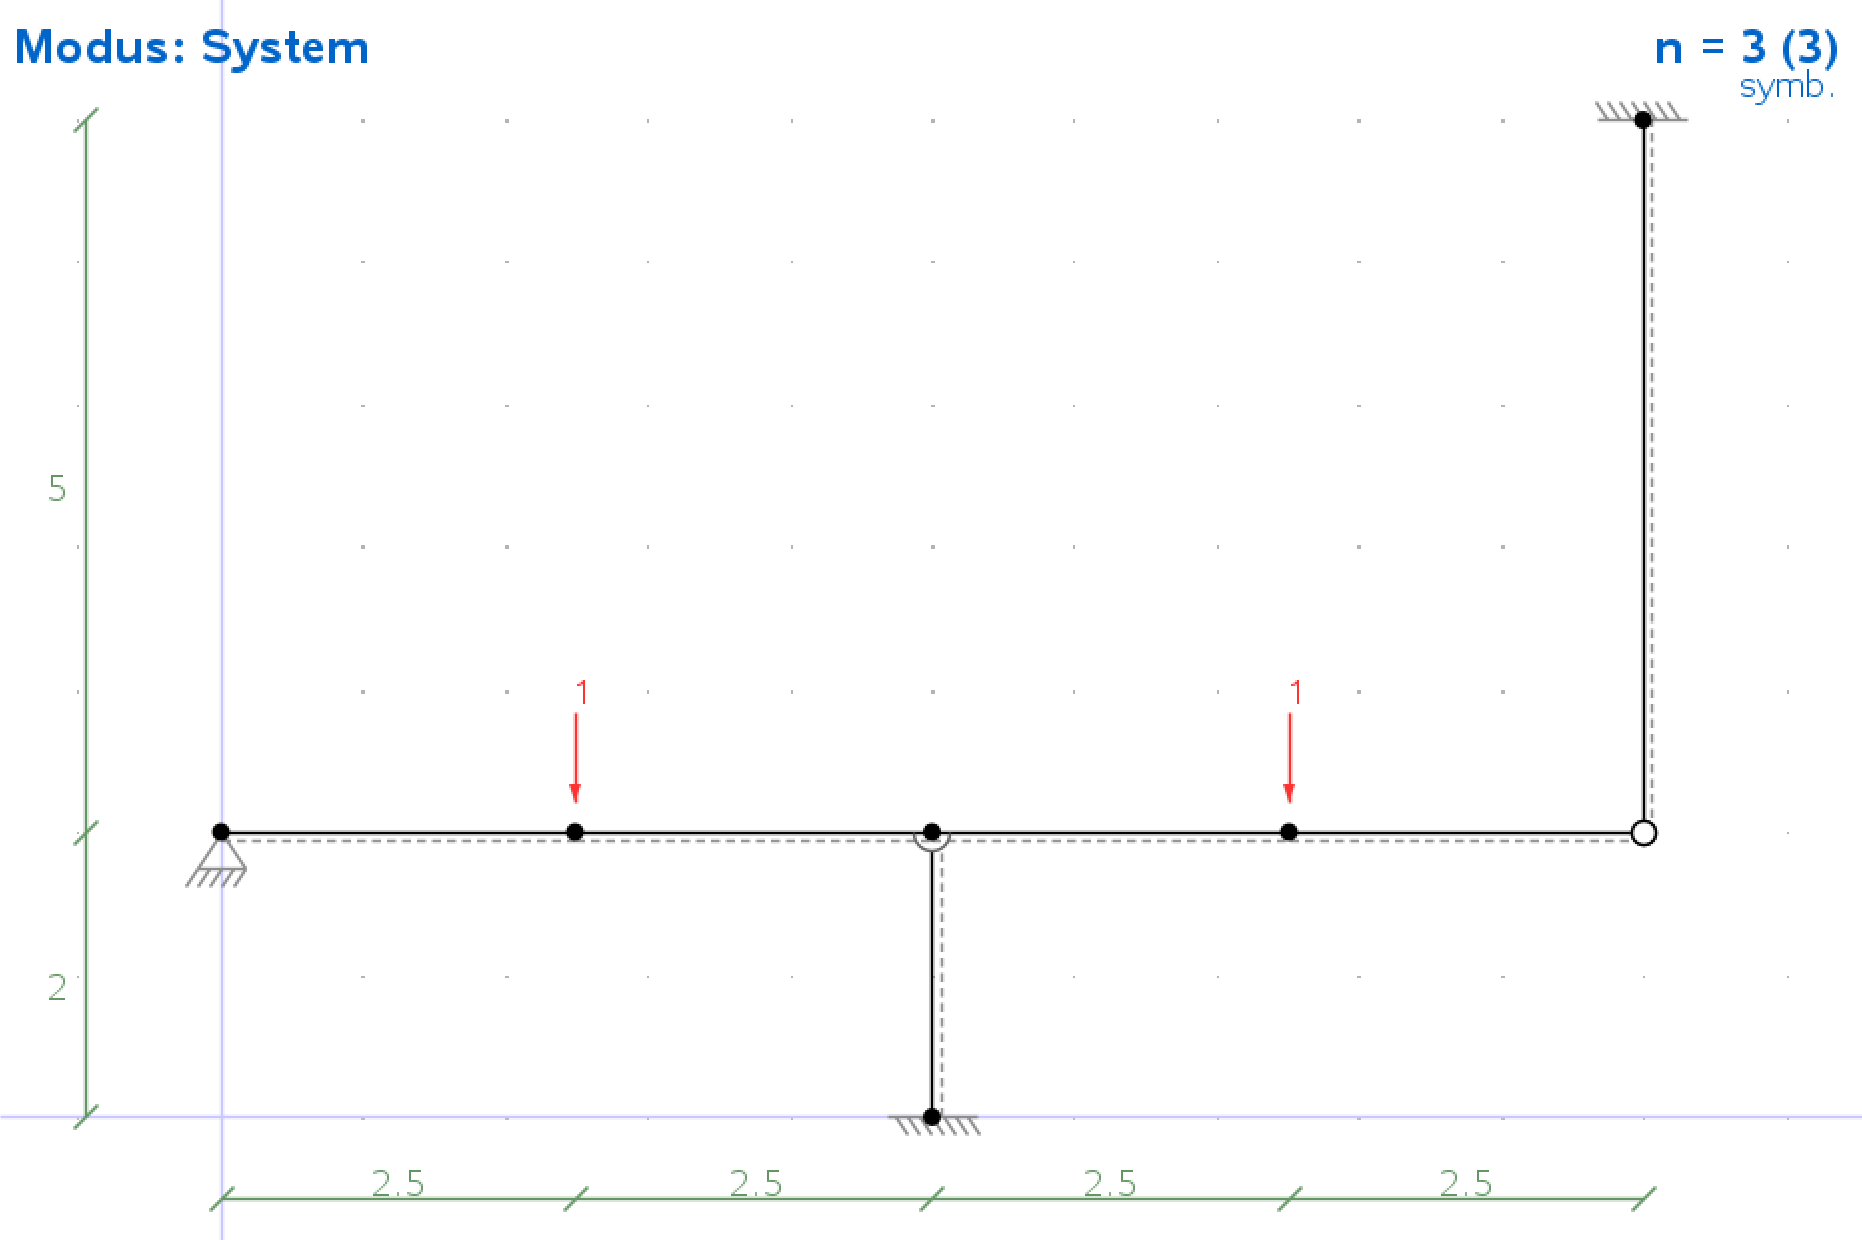
\includegraphics[width=0.5\linewidth]{./fig/TM2/WiSe2021nr4_1.png}
    \caption{TM2 WiSe~20/21, Nr.~4a im Programm}
    \label{fig:verschiebungSystem}
\end{figure}

In den \emph{neuen} Exportfunktionen wird die Temperatur auch symbolisch miteinberechnet.
Um also ann die Verschiebung des rechten unteren Knoten zu kommen lässt sich das entweder über die obere
Knotenexportfunktion machen, über die Biegelinie des rechten horizontalen Stabes oder über die Längsverschiebungsfunktion
des rechten vertikalen Stabes. Über den CAS Befehl \code{solve()} lässt sich die Temperatur direkt ausrechnen 
(vgl. Abb.~\ref{fig:verschiebungErgebniss}). Ich habe hier die Tempertur $dt$ genant (nur $T$ ist wie bereits erwähnt nicht erlaubt),
die Variable nach der aufgelöst werden soll muss der \code{solve()} Funktion als zweites Argument mit gegeben werden.

\begin{figure}[htbp]
    \centering
    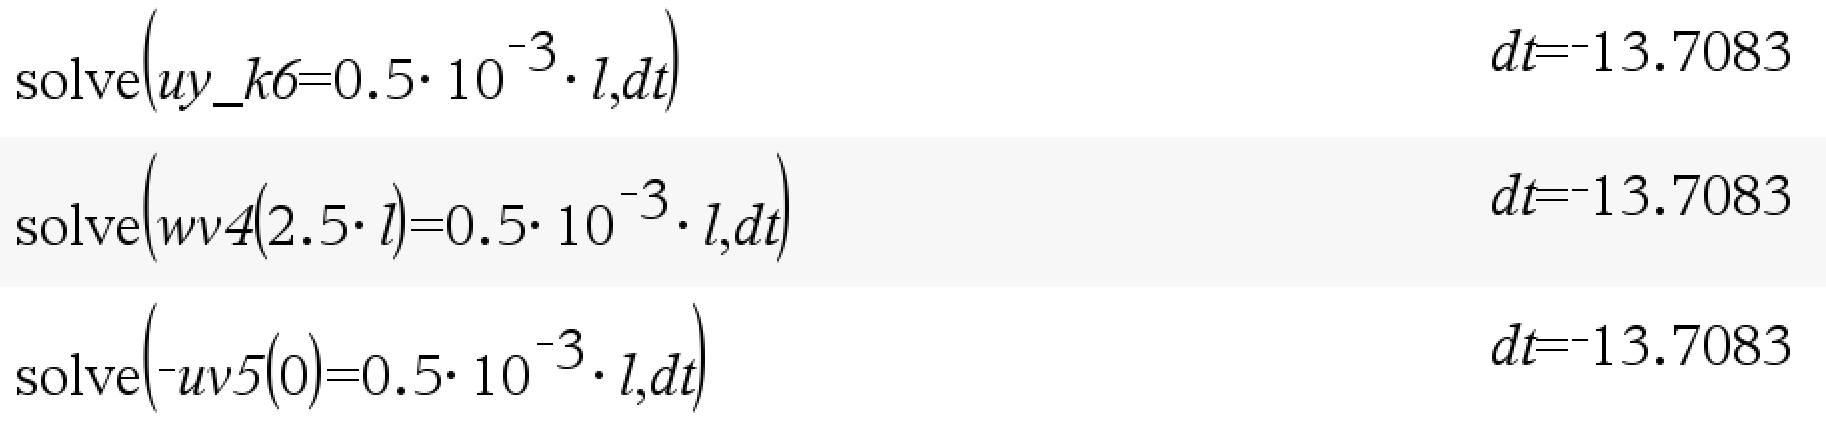
\includegraphics[width=0.5\linewidth]{./fig/TM2/WiSe2021nr4_2.png}
    \caption{Lösung von TM2 WiSe~20/21, Nr.~4a}
    \label{fig:verschiebungErgebniss}
\end{figure}

Der Zweite Teil der Aufgabe lässt sich auch im Programm lösen (Abb.~\ref{fig:VerschiebungTemp}), jedoch gibt es auch hier
ein paar Feinheiten. Ein deratiges System zu speichern kann sich lohnen. Auch hier gelten natürlich die gleichen Hinweise zu den Einheiten.

\begin{figure}[htbp]
    \centering
    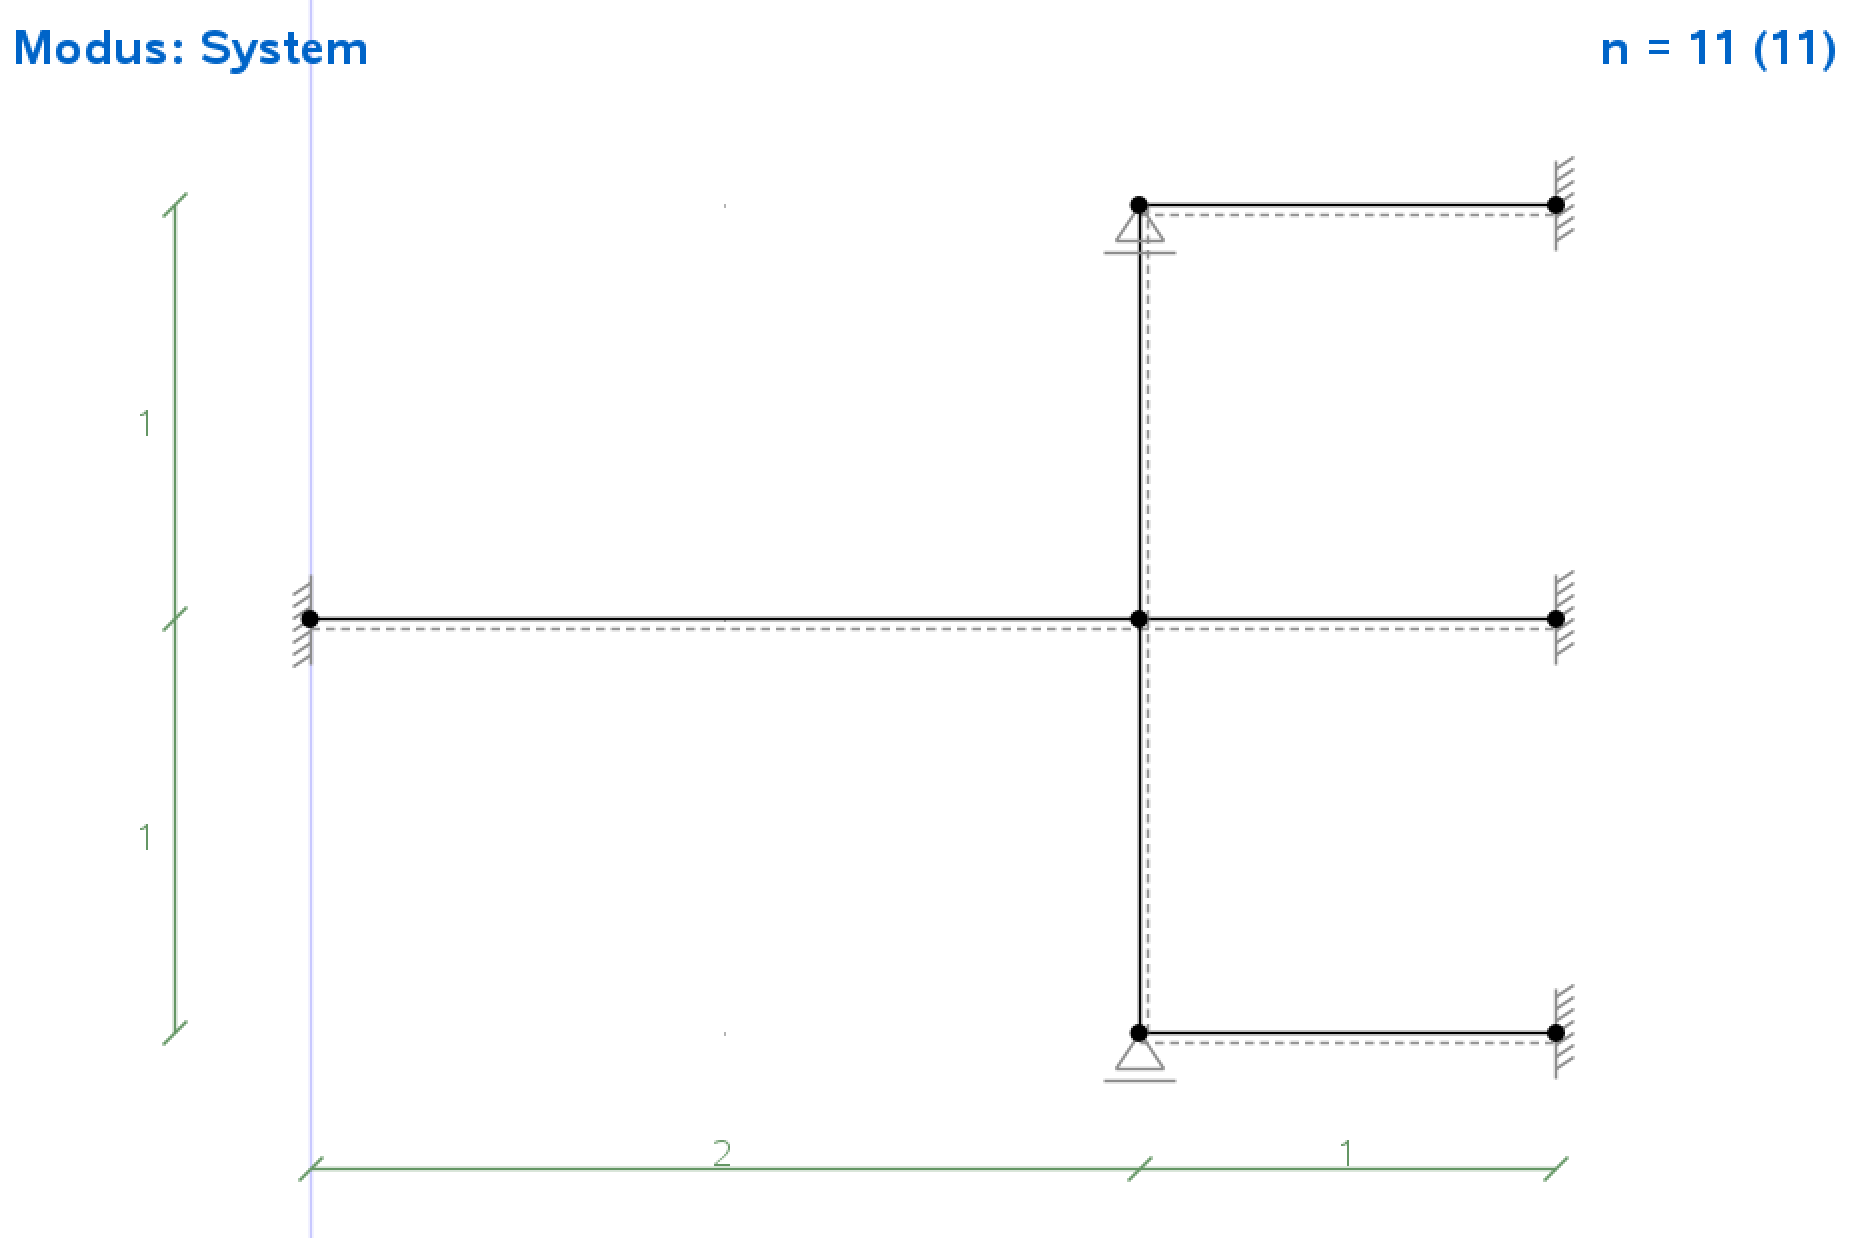
\includegraphics[width=0.5\linewidth]{./fig/TM2/WiSe2021nr4_3.png}
    \caption{TM2 WiSe~20/21, Nr.~4b im Programm}
    \label{fig:VerschiebungTemp}
\end{figure}

Da das Programm nur schnittgrößen direkt berechnet müssen diese noch in Spannungen umgerechnet werden, dafür gibt es in diesem Fall
zwei Möglichkeiten (vgl. Abb.\ref{fig:TM2WiSe2021Nr4b}). Entweder man rechnet die Spannunge direkt über die Schnittkraftverläufe aus,
oder über die Ableitung der Verschiebungsfunktion. Für die zweite Methode muss jedoch darauf geachtet werden den Temperatur Anteil
korrekt zu verrechnen.\\
Erstere Methode ist für Aufgaben mit Zahlenwerten auf jeden Fall die Einfachere, für Aufgaben mit symbolischen Temperatur Werten muss jedoch
die zweite Methode gewählt werden, da die Schnittkraftverläufe diese nicht auf die gewünschte Art berücksichtigen.

\begin{figure}[htbp]
    \centering
    \begin{subfigure}[t]{0.48\textwidth}
        \centering
        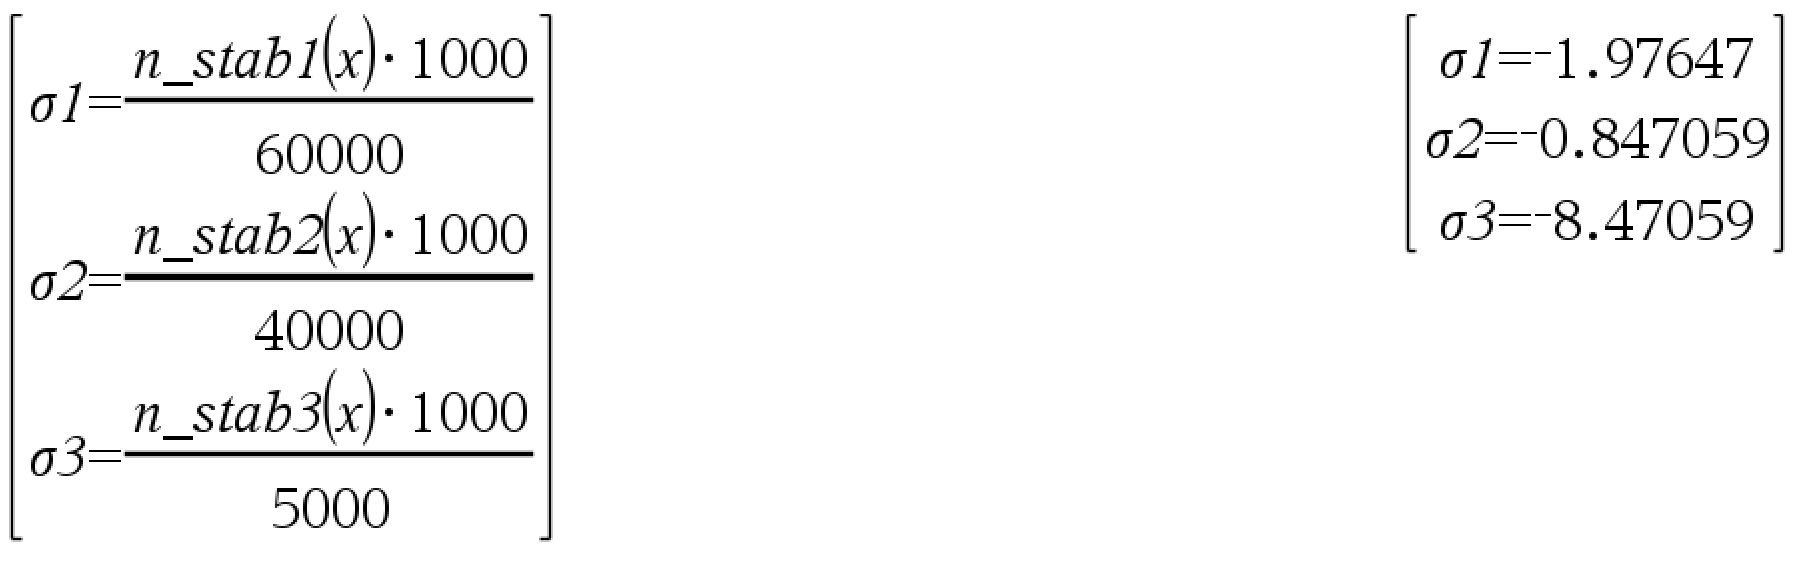
\includegraphics[width=\linewidth]{./fig/TM2/WiSe2021nr4_4.png}
        \caption{Über Schnittgrößen}
    \end{subfigure}
    \hfill
    \begin{subfigure}[t]{0.48\textwidth}
        \centering
        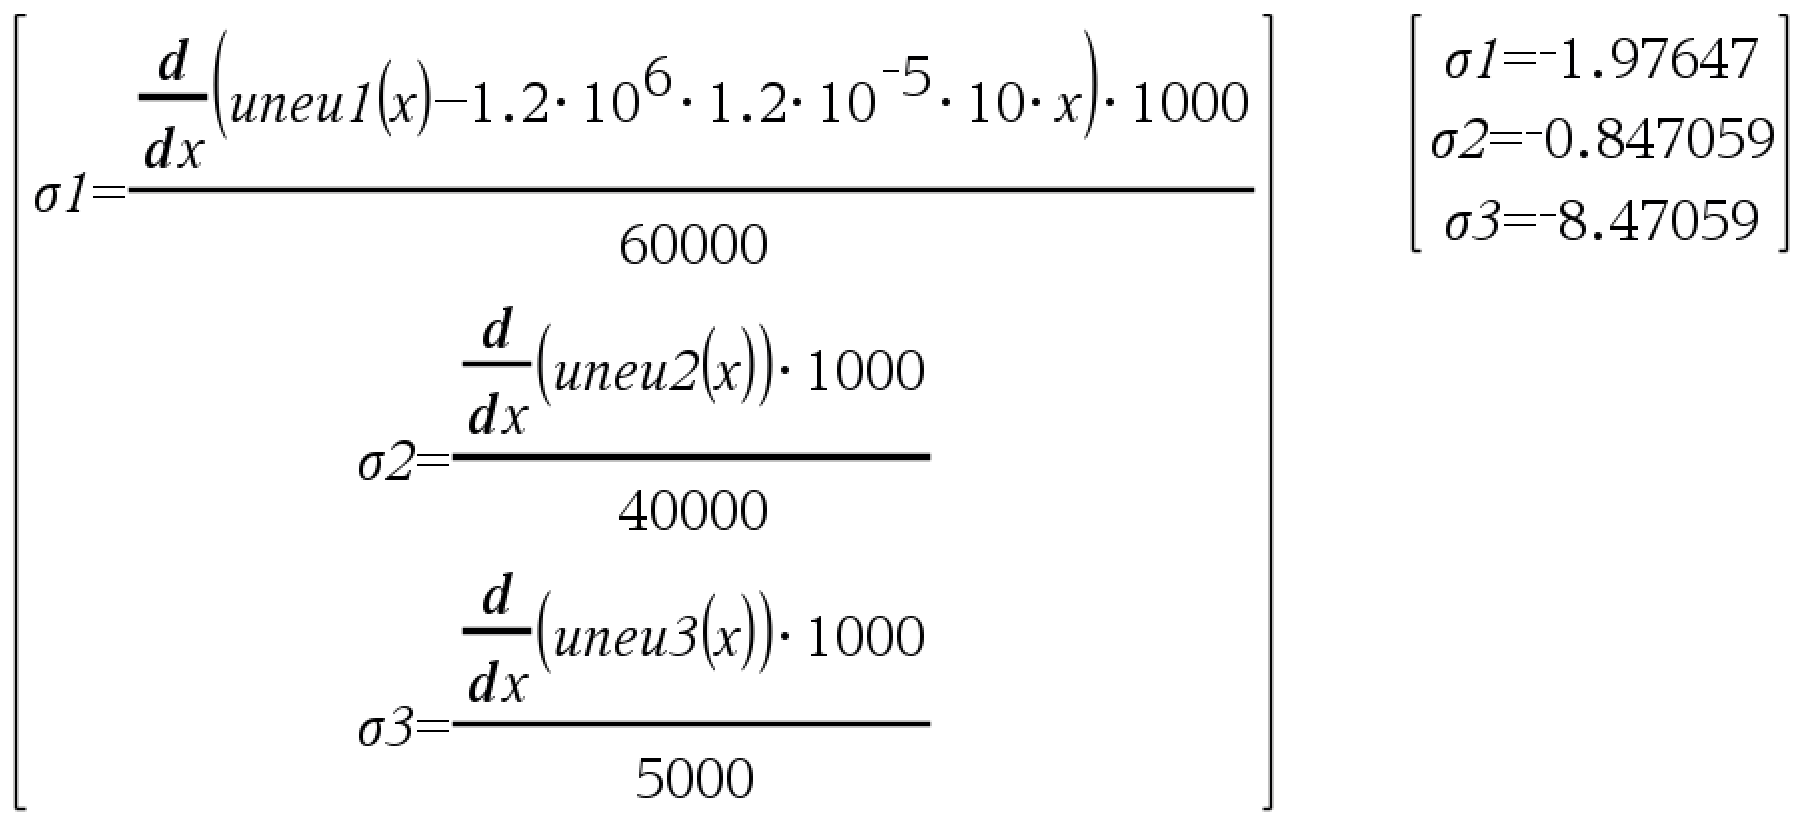
\includegraphics[width=\linewidth]{./fig/TM2/WiSe2021nr4_5.png}
        \caption{Über Verschiebungsfunktion}
    \end{subfigure}
    \caption{Lösung von TM2 WiSe~20/21, Nr.~4b}
    \label{fig:TM2WiSe2021Nr4b}
\end{figure}

Ich will hier anmerken das bei dieser Aufgabenart häufig Hinweise und Warnungen angezeigt werden. Wie z.B. hier auch bei Teilaufgabe a) eine Warnung
zur symbolischen Temperatur. Diese Warnungen sind zwar so konzipiert, dass sie nur angezeigt werden wenn das Programm bzw. ich denke
das etwas falsch eingegeben wurde, jedoch ist es schwer dabei zu vermeiden das auch bei richtiger Eingabe nie eine Warnung oder Hinweis kommt.
Aus diesem Grund empfehele ich, wenn nicht direkt ersichlich ist warum eine Warnung kommt die komplette Eingabe nochmal zu prüfen,
falls diese aber wirklicht korrekt ist sollten auch die Ergebnisse stimmen.


\subsection{Pendelstabannahme (TM2 WiSe 22/23 Nr.~4)} \label{ex:Pendelstabannahme}

\begin{figure}[htbp]
    \centering
    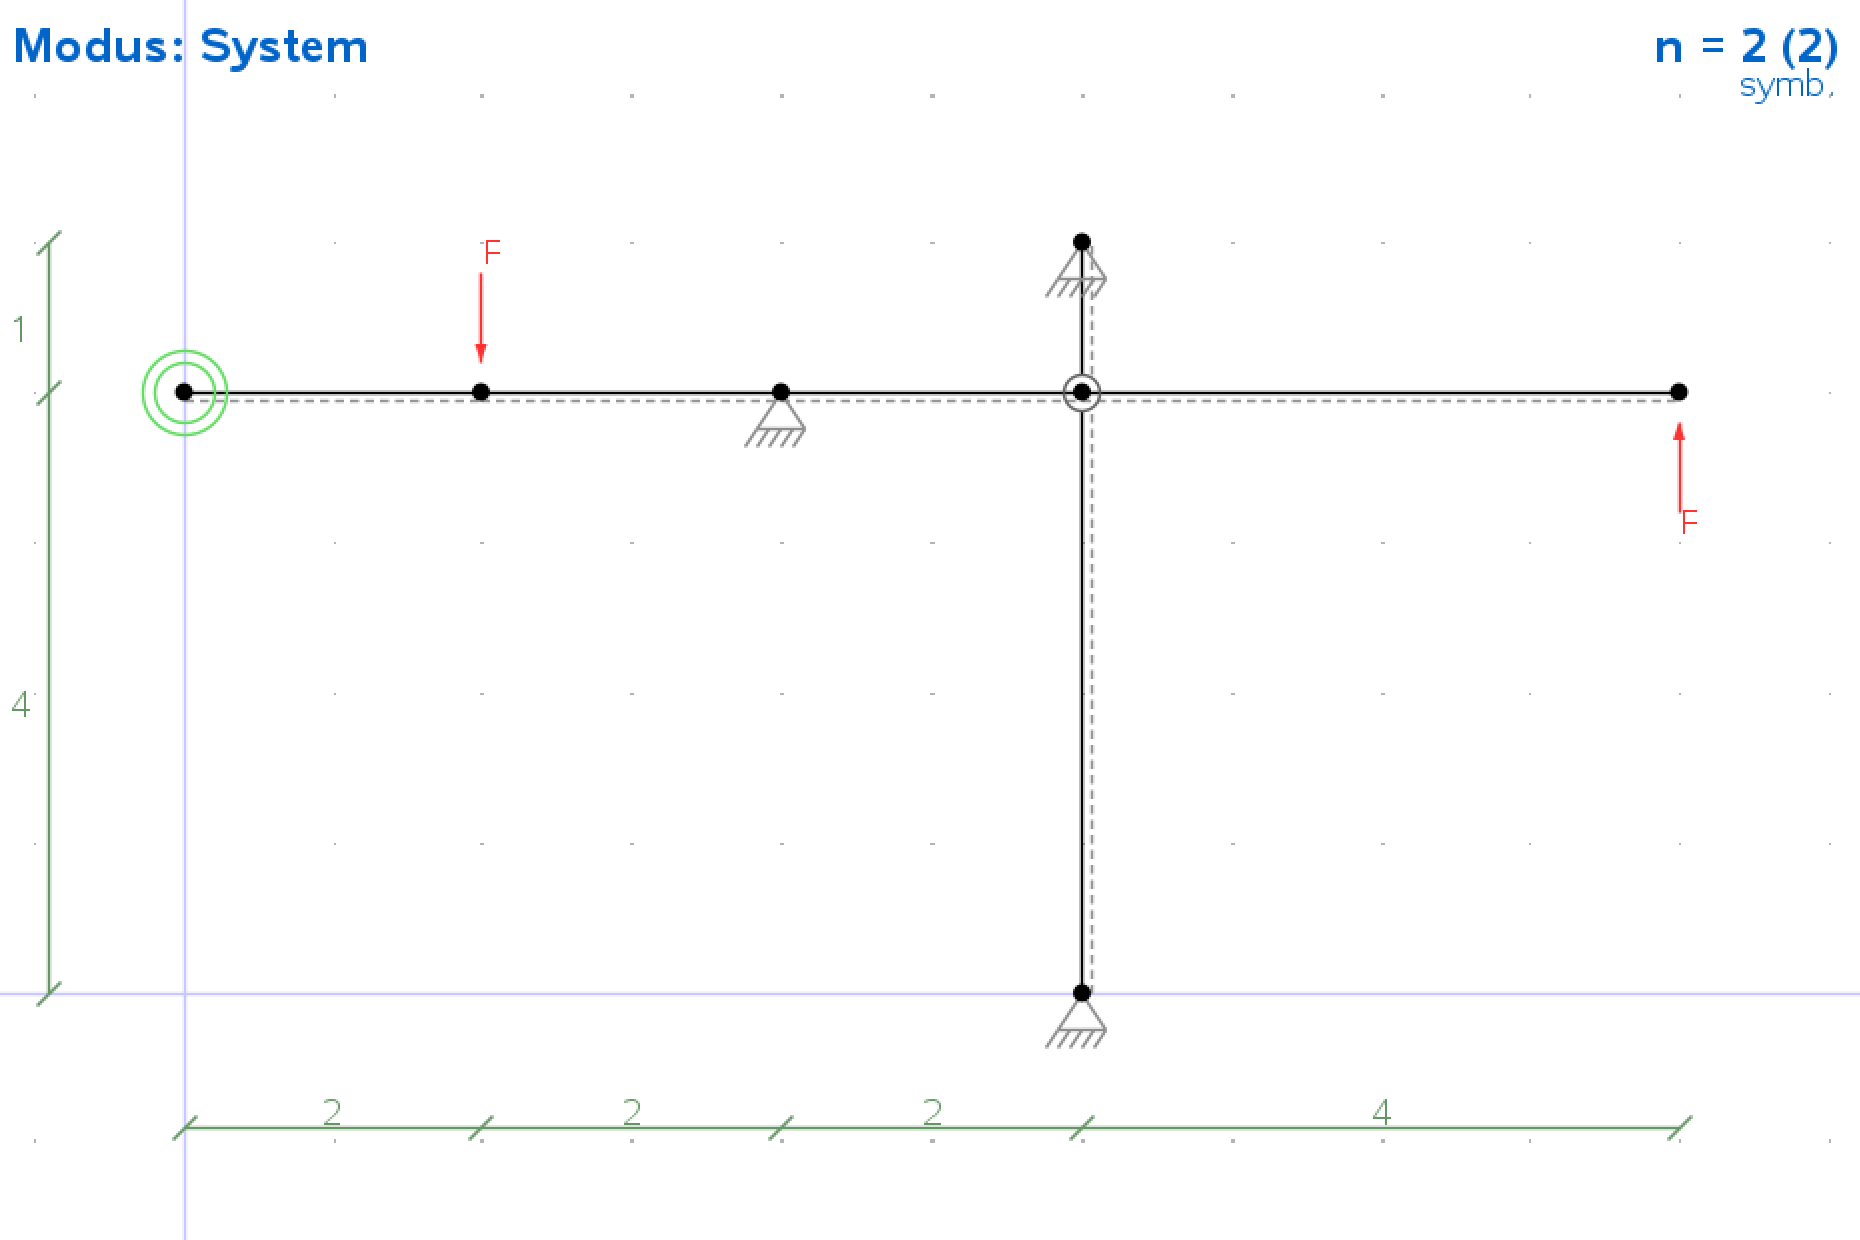
\includegraphics[width=0.7\linewidth]{./fig/TM2/WiSe2223nr4_1.png}
    \caption{TM2 WiSe~22/23, Nr.~4 im Programm}
    \label{fig:Pendelstabsnnahme}
\end{figure}

Wie die Überschrifft vielleicht bereits vermuten lässt muss bei dieser Aufgabe eine Annahme getroffen werden,
die der Zeichnung strenggenommen wiederspricht. Die beiden vertikalen stäbe sollten eigentlich mit einem Angelenk
an den starren Stab angeschlossen werden.\\
Bei einer Handrechnung wird diese Annahme quasi automatisch getroffen, das Programm macht sowas natürlich nicht automatisch.
Um diese Aufgabe mit dem Programm also korrekt zu rechnen müsseb bei den beiden vertikalen stäbe jeweils Angelenke eingebaut werden.
Falls man das nicht macht wirft das Programm eine Warnung bzw. einen Hinweis.

Bei dieser Aufgabe lassen sich die Ergebnisse entweder aus der Ansicht zur Normalkraft 
oder aus dem E-Modus holen (Abb.~\ref{fig:TM2WiSe2223Nr4}).

\begin{figure}[htbp]
    \centering
    \begin{subfigure}[t]{0.48\textwidth}
        \centering
        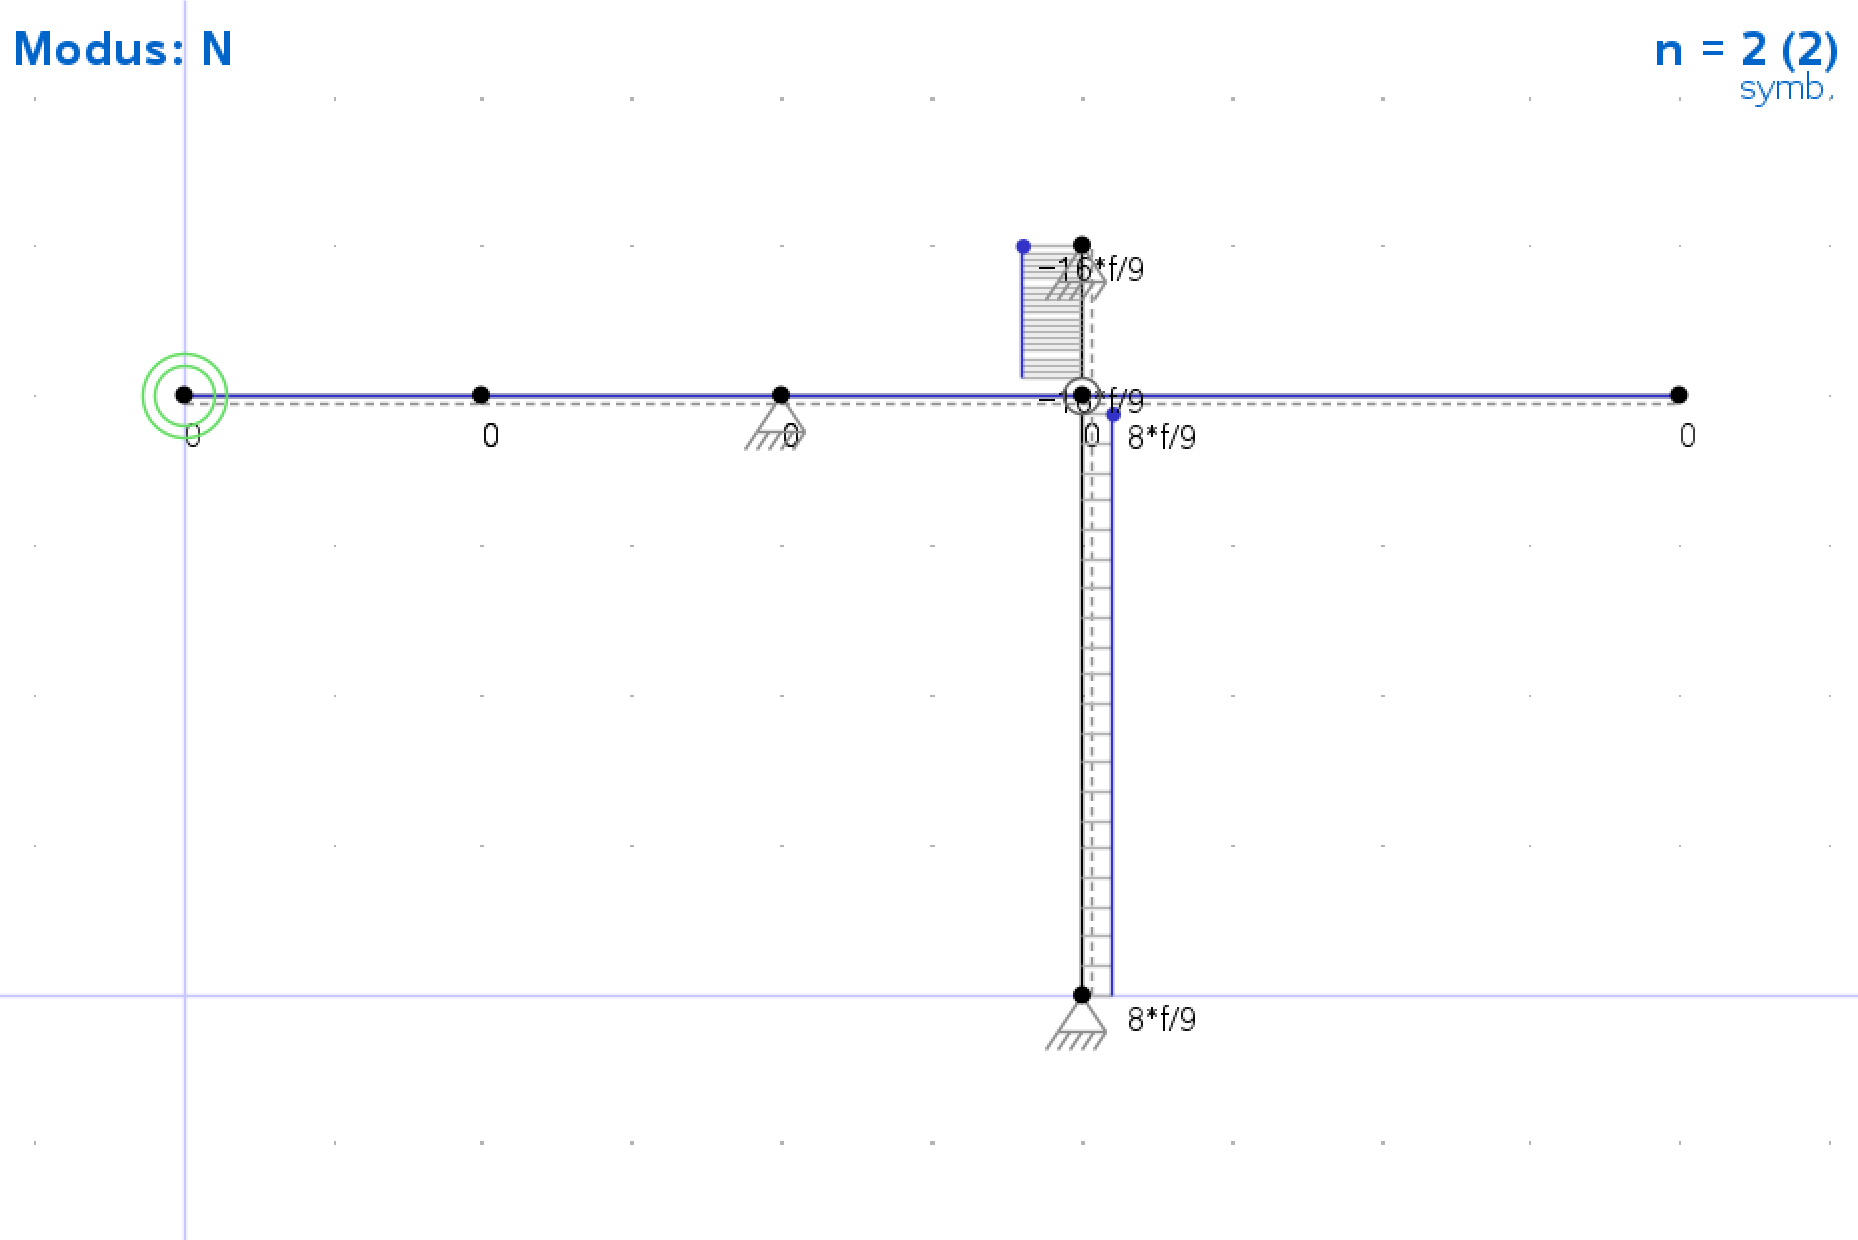
\includegraphics[width=\linewidth]{./fig/TM2/WiSe2223nr4_2.png}
        \caption{Normalkraft}
    \end{subfigure}
    \hfill
    \begin{subfigure}[t]{0.48\textwidth}
        \centering
        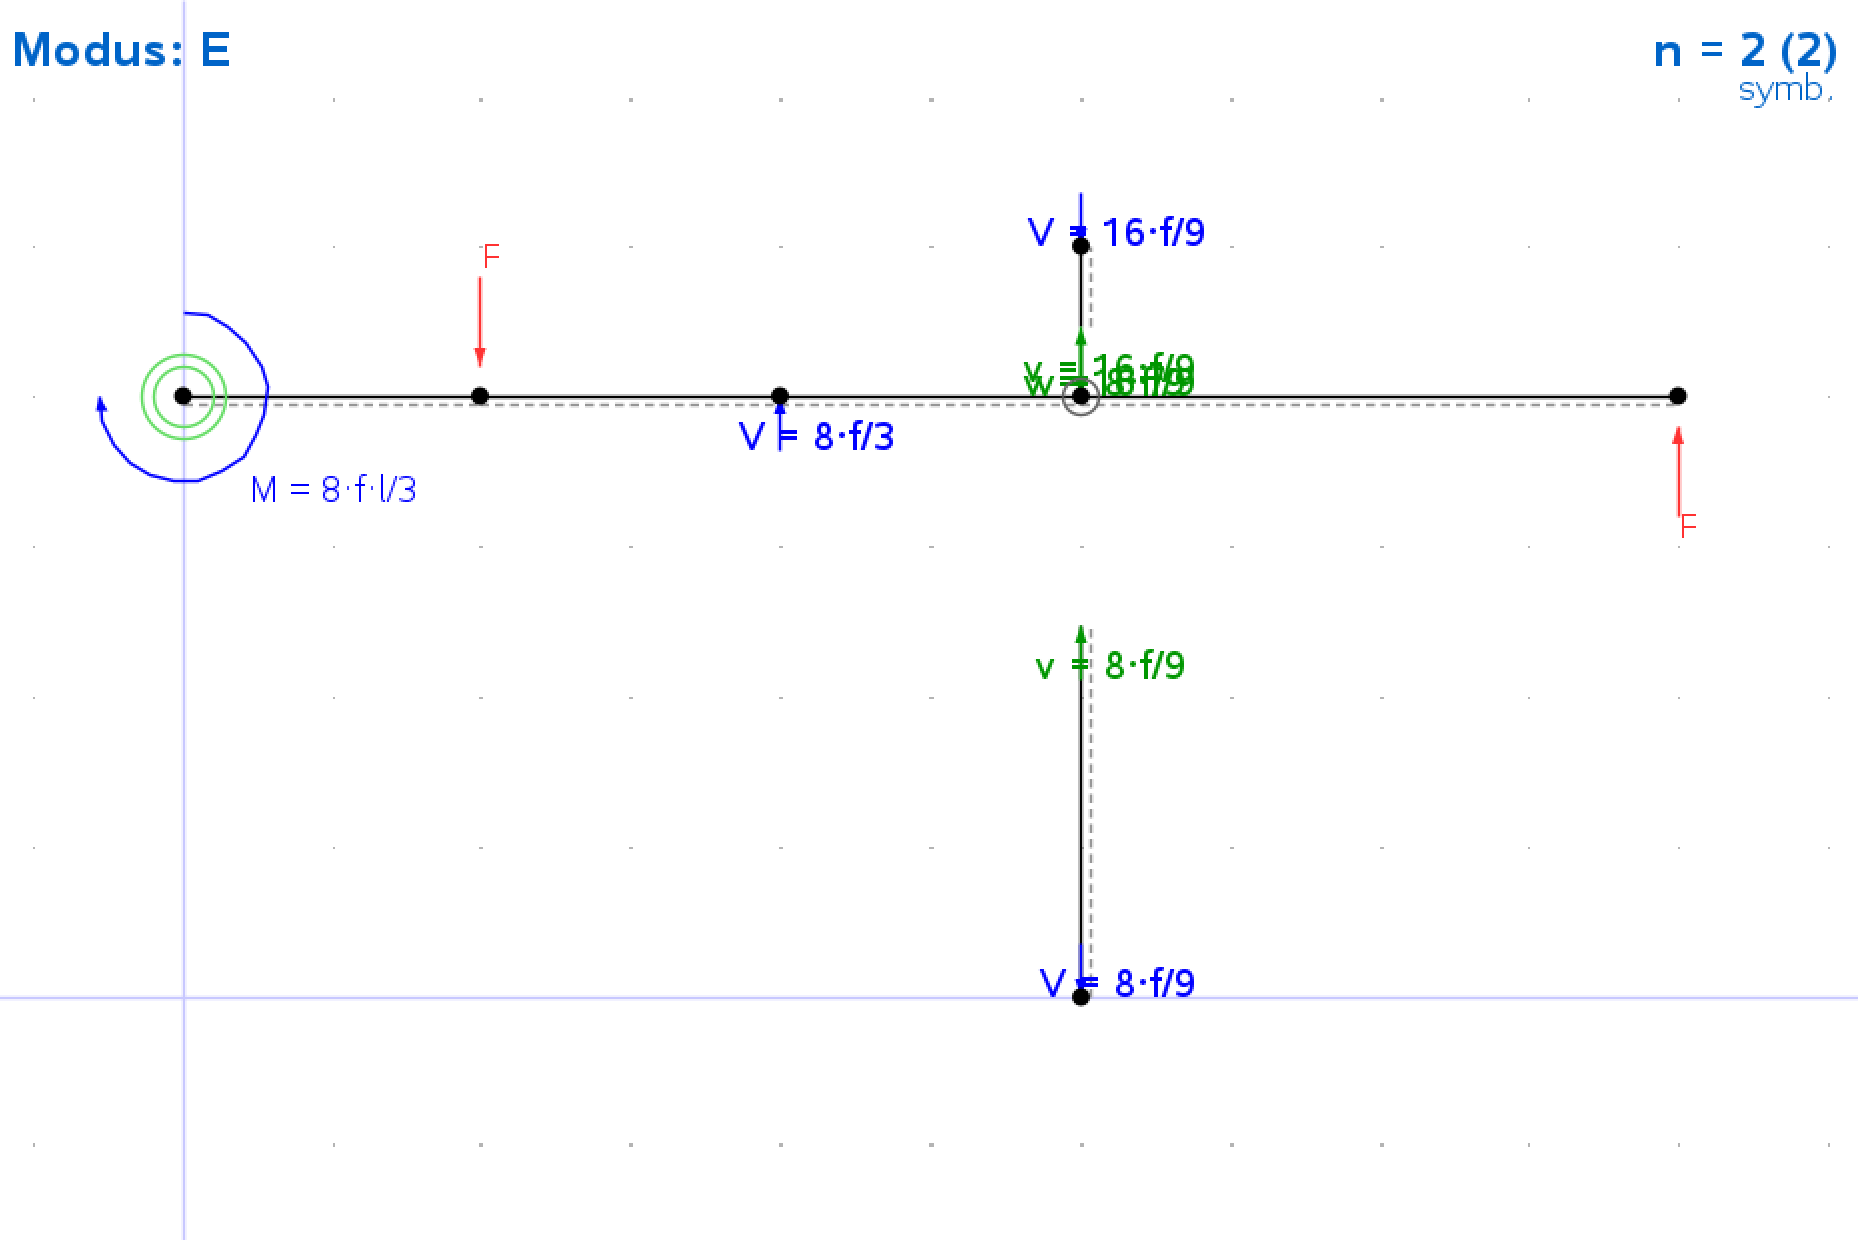
\includegraphics[width=\linewidth]{./fig/TM2/WiSe2223nr4_3.png}
        \caption{E-Modus}
    \end{subfigure}
    \caption{Lösung von TM2 WiSe~22/23, Nr.~4}
    \label{fig:TM2WiSe2223Nr4}
\end{figure}

\textbf{Wichtig} ist, dass das Programm, für symbolische Federn in den Verläufen in seltenen Fällen nicht die richtigen 
Werte ausgibt (Bei symbolischen Temperaturen sowieso nicht).
Zur Sicherheit würde ich deswegen die Schnittgrößen über die \emph{neuen} Verschiebungsfunktionen ermitteln. 
Das dauert zwar gerade für große Systeme länger, ist aber zuverlässiger weil dort wirklich alles symbolisch gerechnet wird 
und eben nicht gepfuscht wird.



\subsection{Schiefe Biegung (TM2 WiSe 25/26 Nr.~8)}

In dieser Aufgbabe sind die Dicken der dünnwandigen Elemente nicht gegeben, da diese abber sowohl für das
FTM als auch für die Lange des Schwerpunkts wichtig sind, müssen diese Werte manuell mit den Werten aus der 
Aufgabenstellung überschrieben werden. Das geht im Obermenue (Taste \taste{o}) auf Seite 3.\\
Für das Zeichnen so eines schiefen Querschnitts empfielt sich ein Rastermaß von z.B. $\frac{1}{\sqrt{2}}$.

\begin{figure}[htbp]
    \centering
    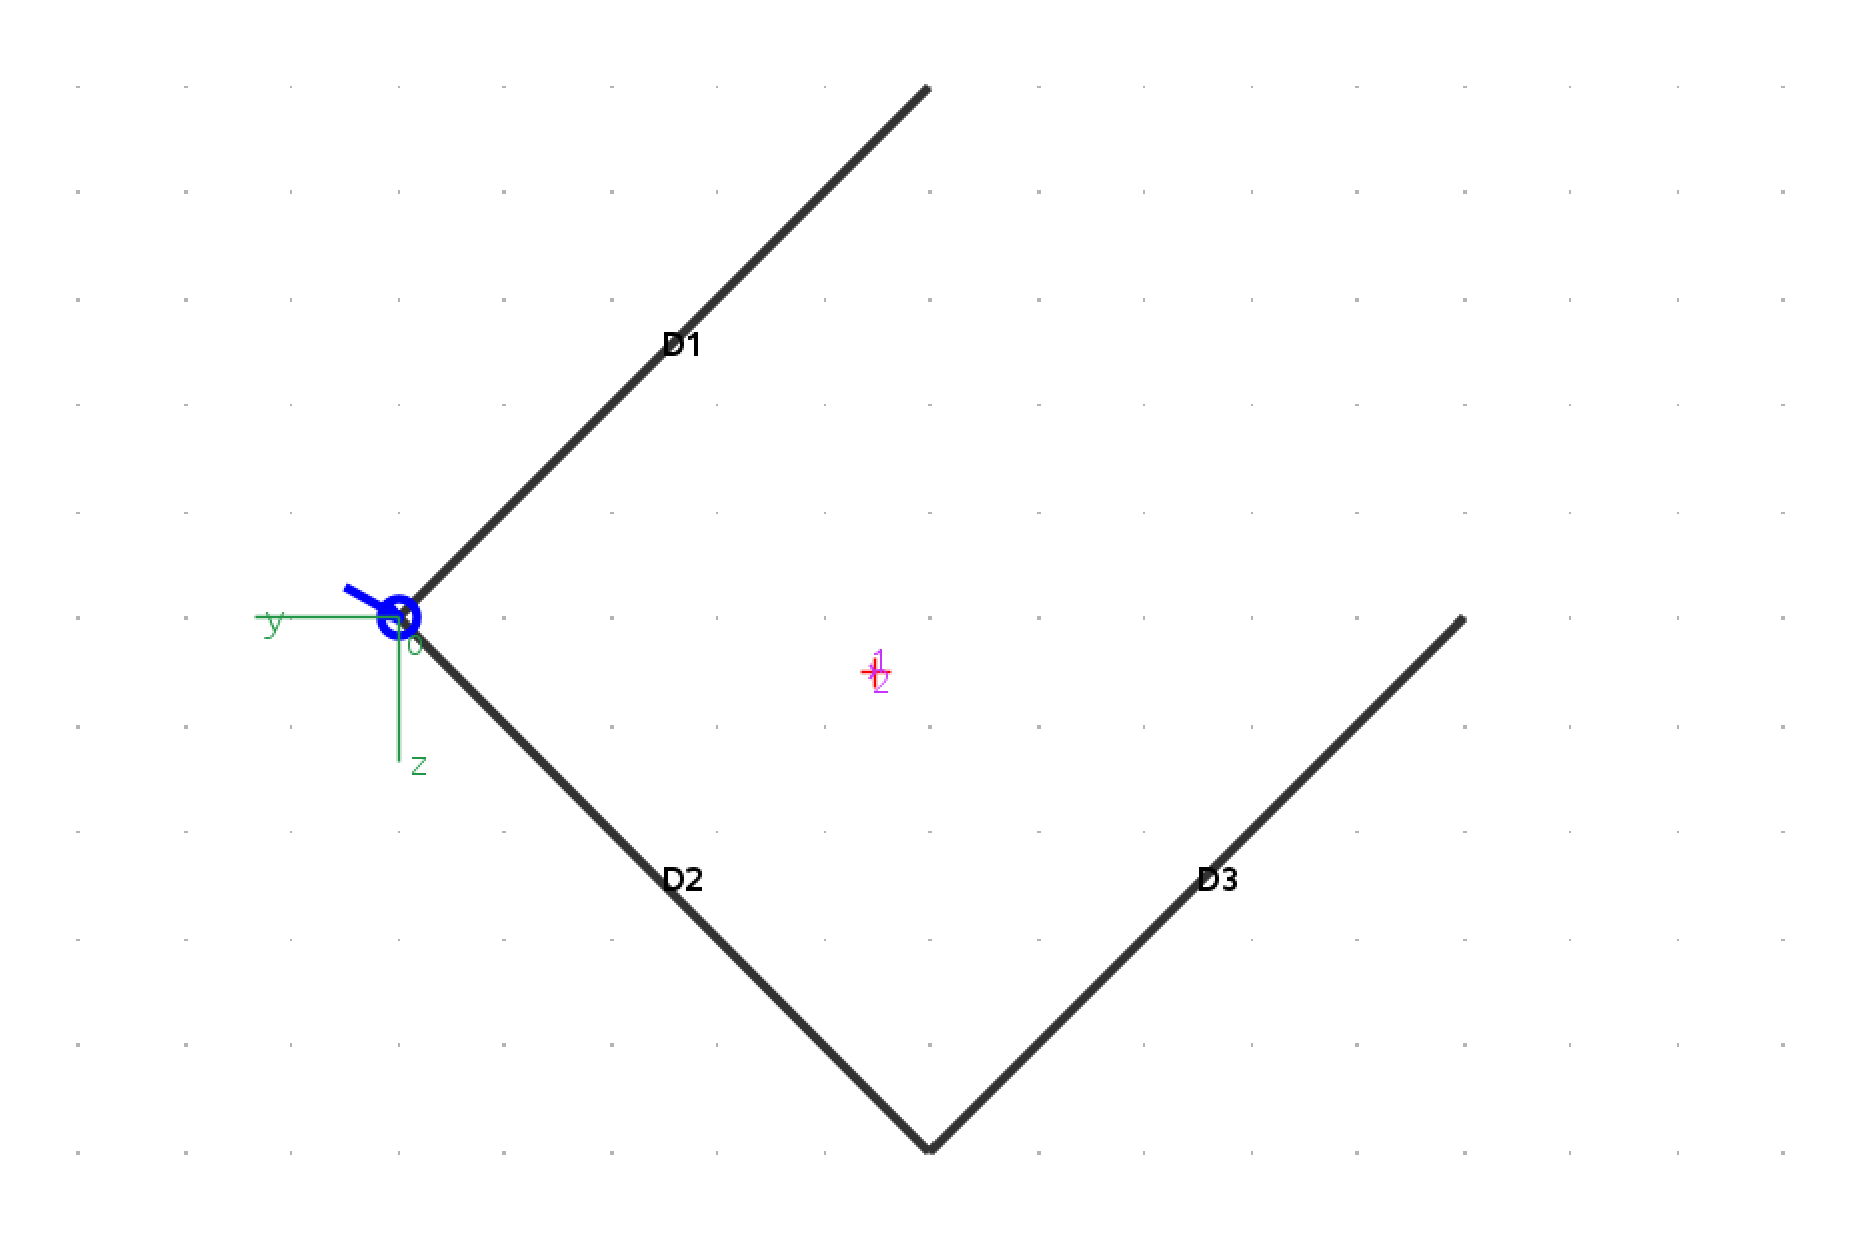
\includegraphics[width=0.7\linewidth]{./fig/TM2/WiSe2526nr8_1.png}
    \caption{TM2 WiSe~25/26, Nr.~8 im Programm}
    \label{fig:TM2WiSe2526Nr8_1}
\end{figure}

Bei dieser Aufgabe braucht man die $\sigma_x$-Berechnung. Um die Normalkraft hier richtig einzuberechnen
muss die Resultierende der Streckenlast über die halbe Länge berechnet werden, also: 
$R=0,1~\frac{\text{kN}}{cm}\cdot100~\text{cm}$.
Für die Kraft muss also $F_y=-500~\text{N}$, $F_z=300~\text{N}$ und $F_x=10000~\text{N}$ eingegeben werden.

Nach dem Aufruf der Berechnung werden noch ein paar Werte abgefragt. Für die ersten Drei muss Null eingetragen werden.
Man hätte auch keine Kraft platzieren können, die Normalkraft und Momente handisch ausrechnen können und diese dann in diese Felder eintragen können.
Das Ergebniss ist das gleiche.\\
Für $\Delta x$ muss $100~\text{cm}$ eingetragen werden, das ist der Abstand zwischen dem gezeichneten Schnitt und dem betrachteten Schnitt.
Das Programm rechnet dann also automatisch die Momente aus der Querkraft aus. Dieses Feature funktioniert natürlich nur, wenn zwischen dem gezeichneten und berechneten Schnitt
keine Weiteren Einflüsse wie Lager oder Kräfte Angreiffen, dann kommt man nicht darum herum $N$, $M_y$ und $M_z$ händisch auszurechnen und einzutragen.

Die Ergebnisse sind in Abbildung \ref{fig:TM2WiSe2526Nr8_2} dargestellt.

\begin{figure}[htbp]
    \centering
    \begin{subfigure}[t]{0.48\textwidth}
        \centering
        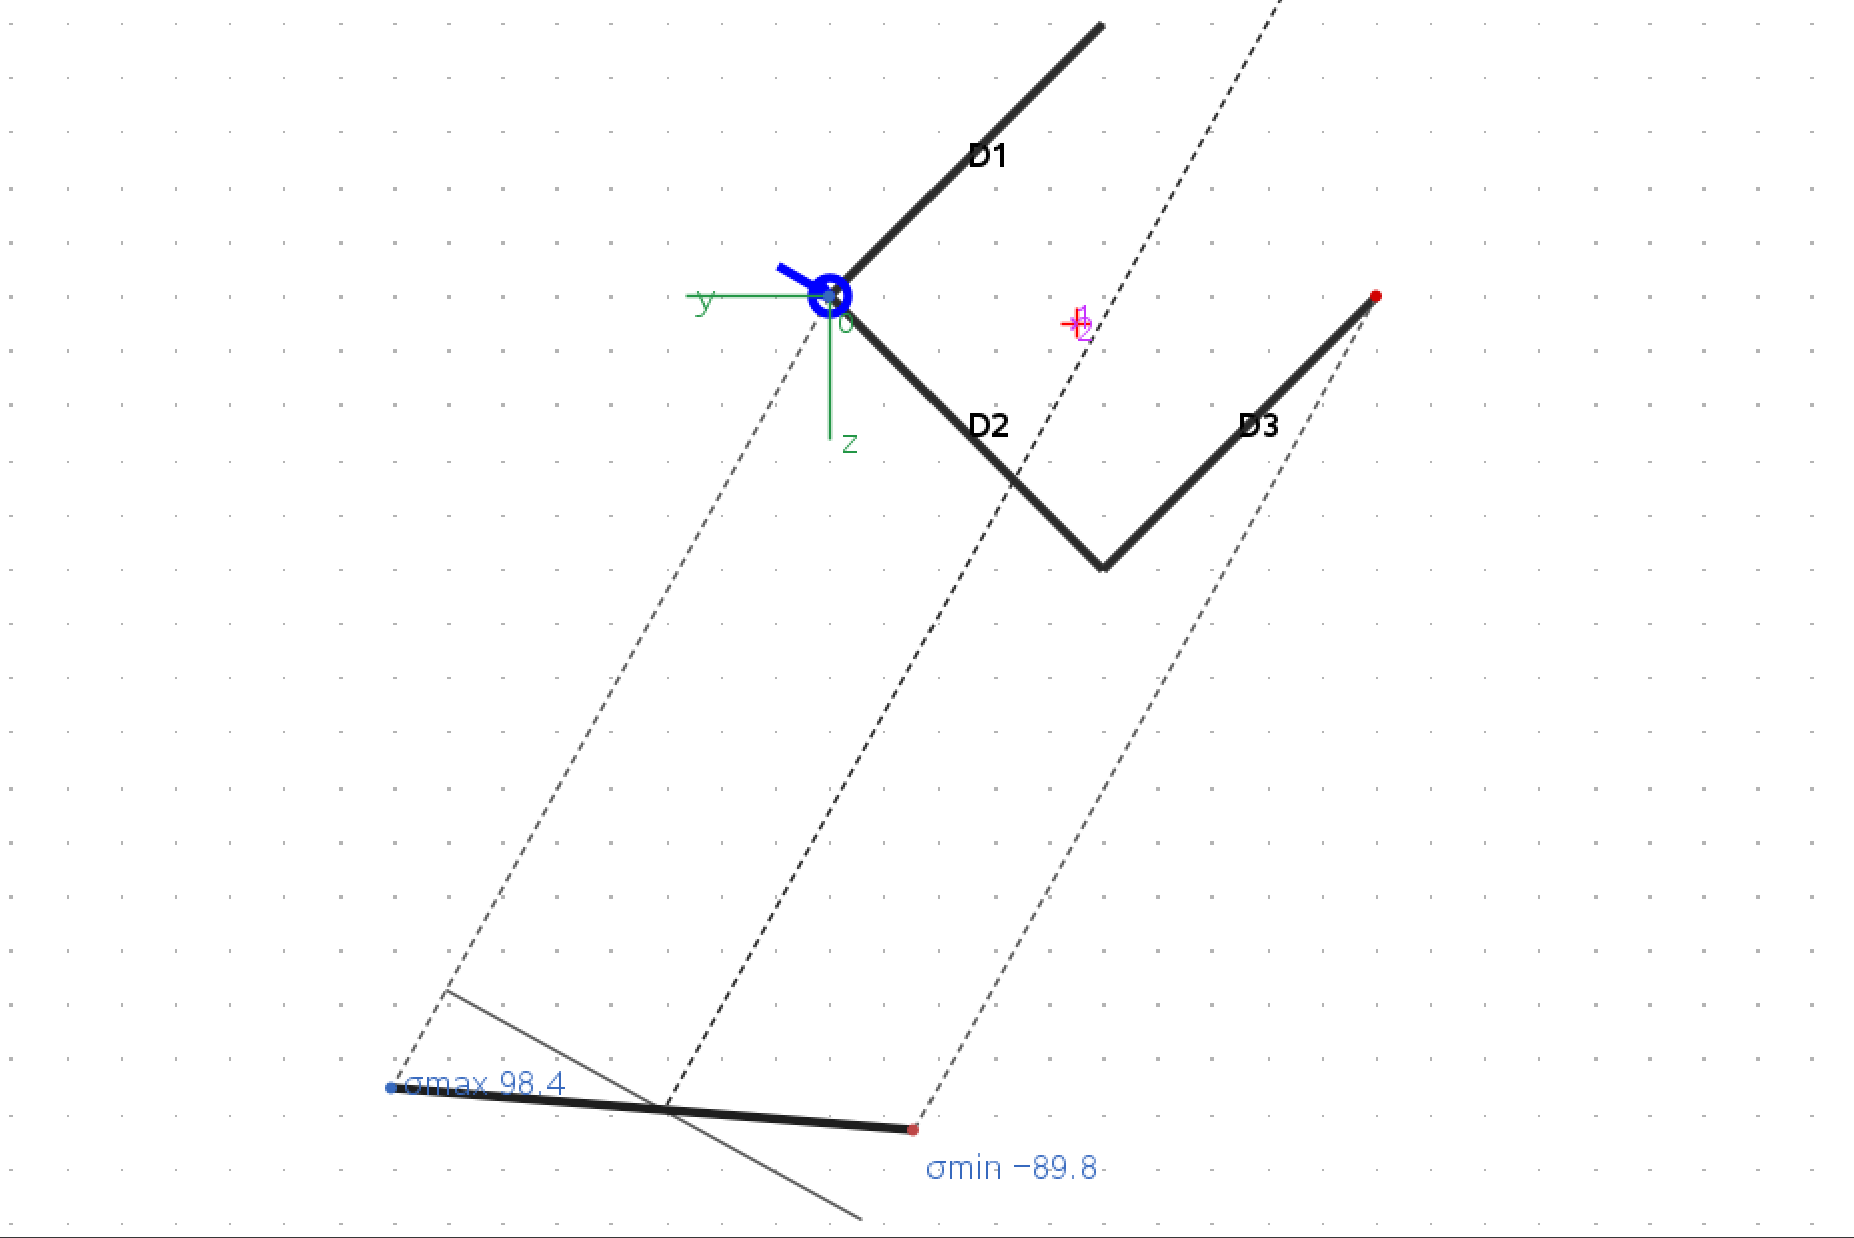
\includegraphics[width=\linewidth]{./fig/TM2/WiSe2526nr8_2.png}
        \caption{Spannungsverlauf}
    \end{subfigure}
    \hfill
    \begin{subfigure}[t]{0.48\textwidth}
        \centering
        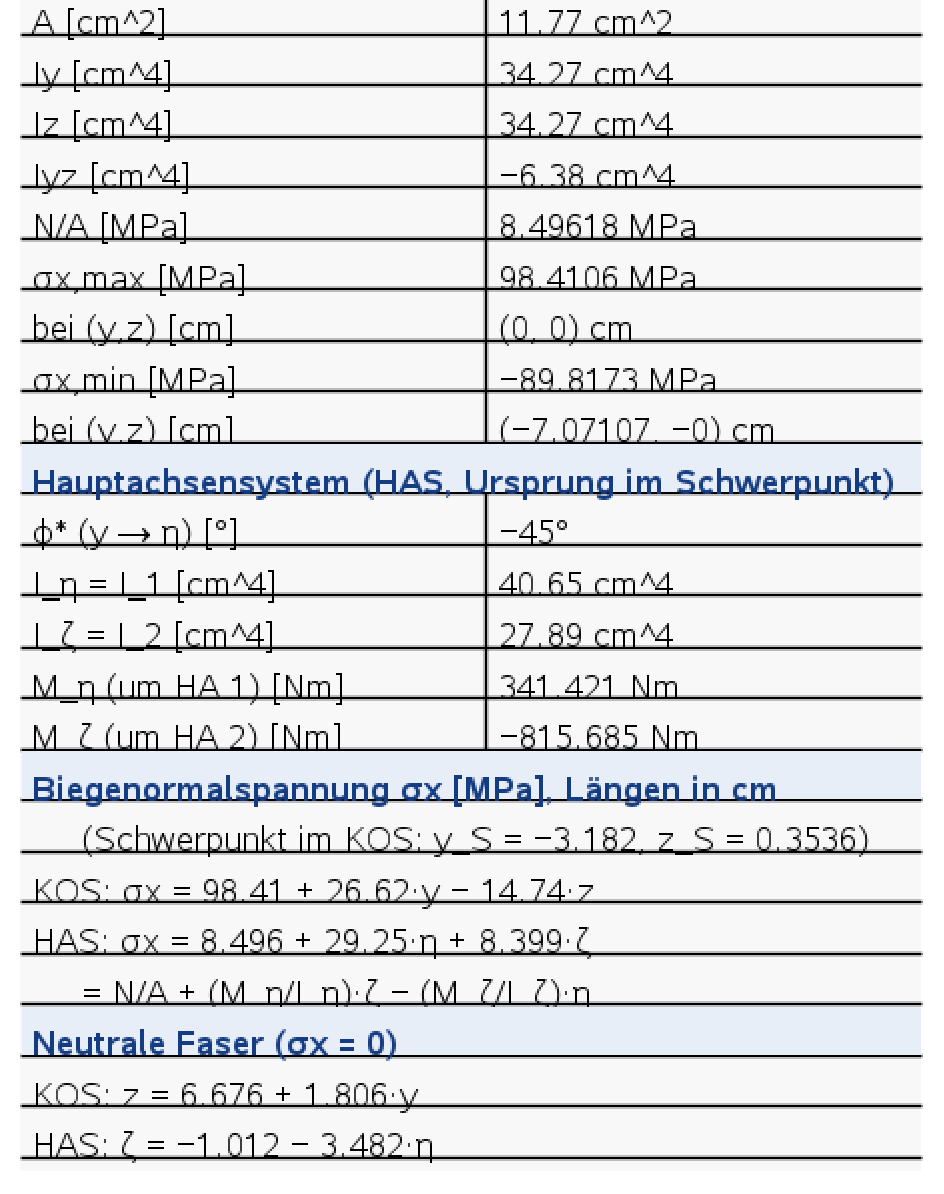
\includegraphics[width=\linewidth]{./fig/TM2/WiSe2526nr8_3.png}
        \caption{Tabellen übersicht}
    \end{subfigure}
    \caption{Lösung von TM2 WiSe~25/26, Nr.~8}
    \label{fig:TM2WiSe2526Nr8_2}
\end{figure}

Ich will anmereken, dass des öfteren bei Aufgaben Querschnittswerte gegeben sind, die nicht zur Bemaßung in der Zeichnung passen,
ob das absichtlich so ist konnte mir leider keiner sagen. Es ist also immer sinnvoll das einmal gegen zu prüfen und die Werte evtl. zu überschreiben.
Was die ISD-Musterlösung bei dieser Aufgabe gerechnet hat, ist mir nicht ganz klar. Meines Verständnisses nach wurde hier mit einem
Schwerpunkt für die Momente aus Normalkraft gerechnet, der genau in der Mitte des U profiels liegt, sodass die Normalkraft um die $y$-Achse kein Moment erzeugt.

\subsection{Schiefe Biegung/Kernfäche (TM2 WiSe21/22 Nr.~8)}



\subsection{MSK (TM2 WiSe 21/22 Nr.~3)}

Zu dieser Aufgabe gibt es eigentlich nicht besonders viel zu sagen, man gibt die gegebenen Werte ein und das Programm
füllt in grün die restlichen Werte auf (Abb.~\ref{fig:TM2WiSe2122Nr3_1}).

\begin{figure}[htbp]
    \centering
    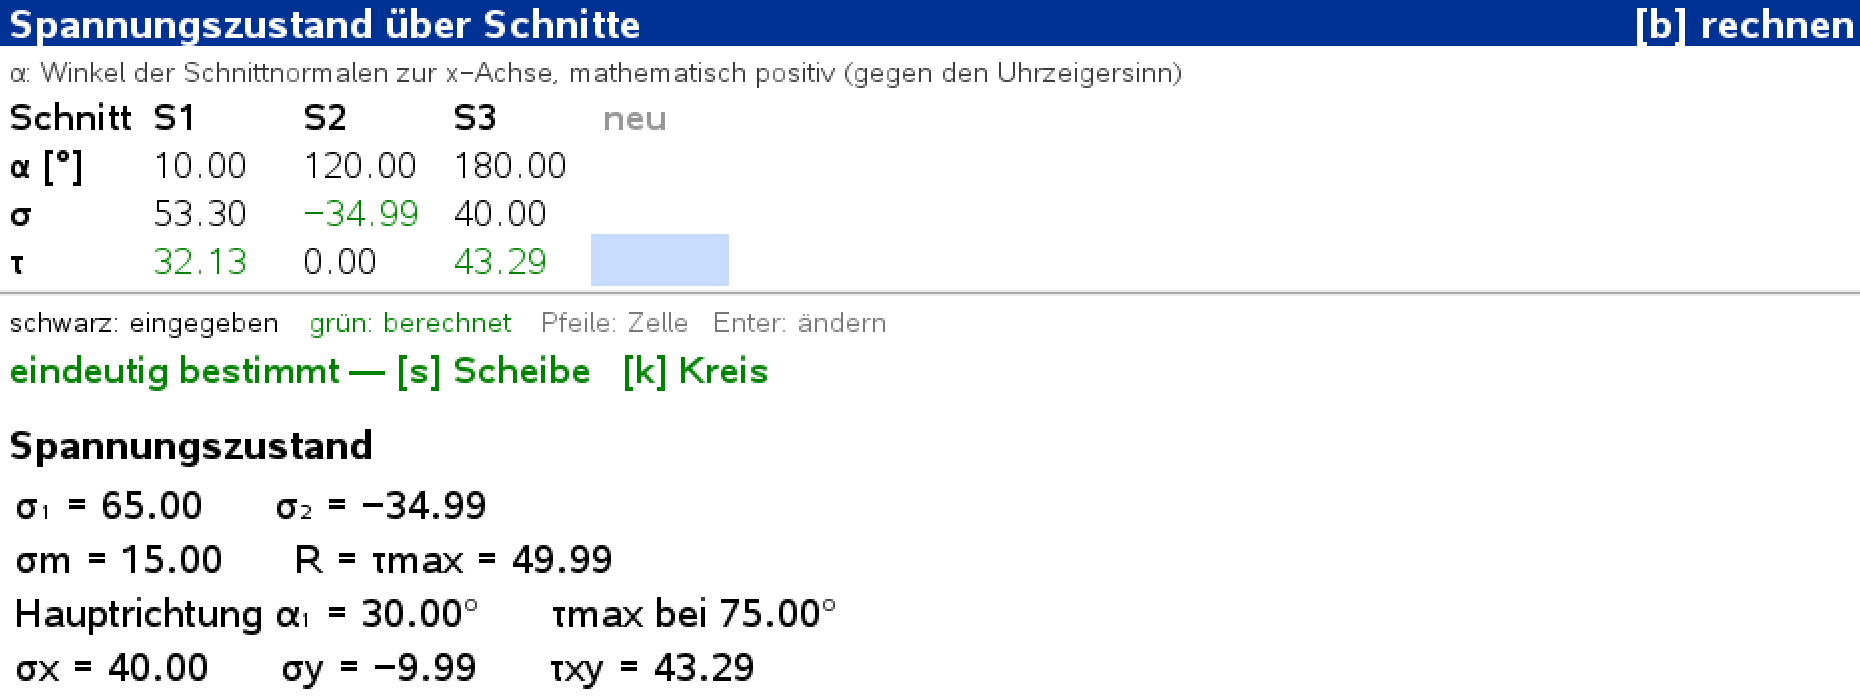
\includegraphics[width=0.7\linewidth]{./fig/TM2/WiSe2122nr3_1.png}
    \caption{TM2 WiSe~21/22, Nr.~3 im Programm}
    \label{fig:TM2WiSe2122Nr3_1}
\end{figure}

Danach bekommt man mit den Tasten \taste{s} und \taste{k} die beiden wichtigen Ansichten (Abb.~\ref{fig:TM2WiSe2122Nr3_2}).


\begin{figure}[htbp]
    \centering
    \begin{subfigure}[t]{0.48\textwidth}
        \centering
        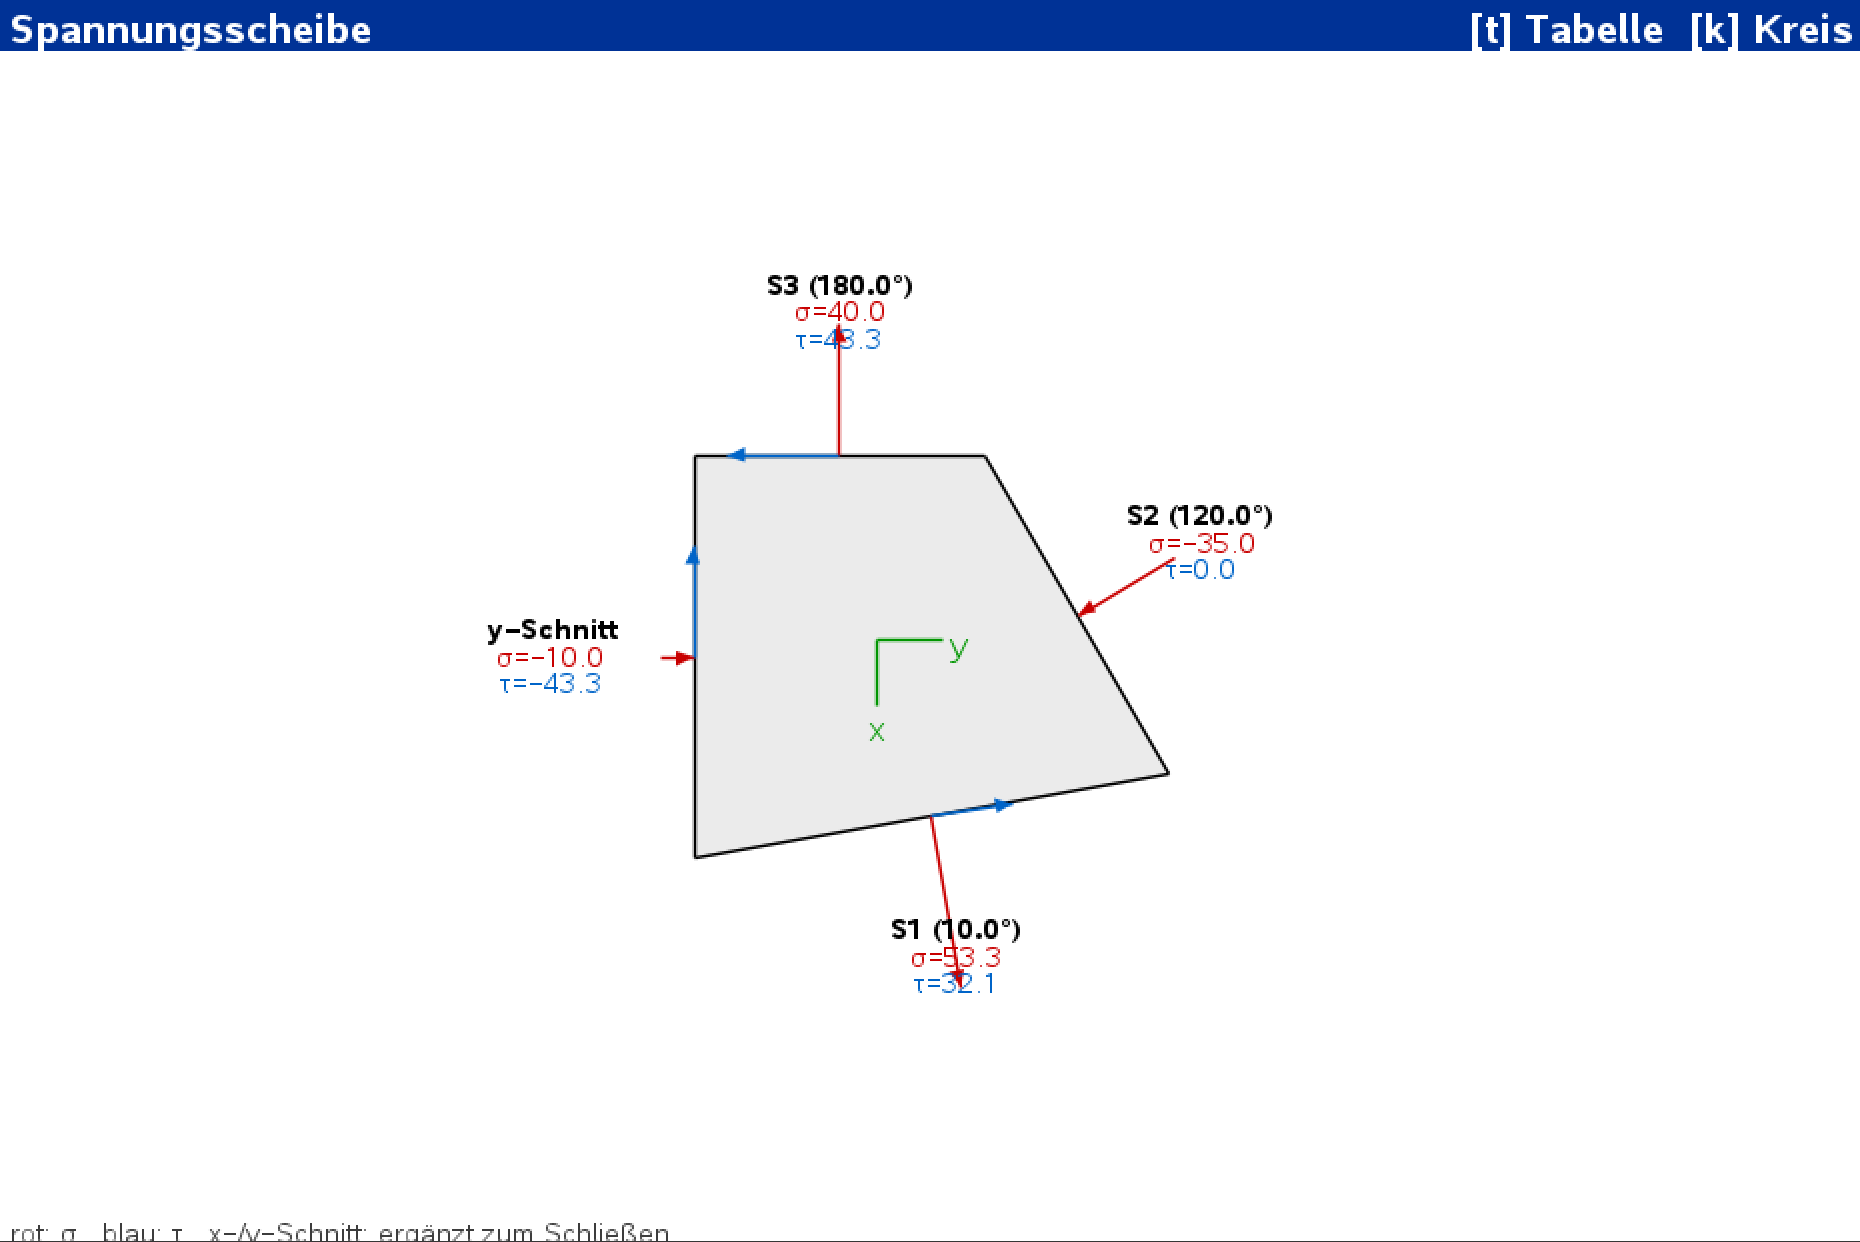
\includegraphics[width=\linewidth]{./fig/TM2/WiSe2122nr3_2.png}
        \caption{Spannungs-Scheibe}
    \end{subfigure}
    \hfill
    \begin{subfigure}[t]{0.48\textwidth}
        \centering
        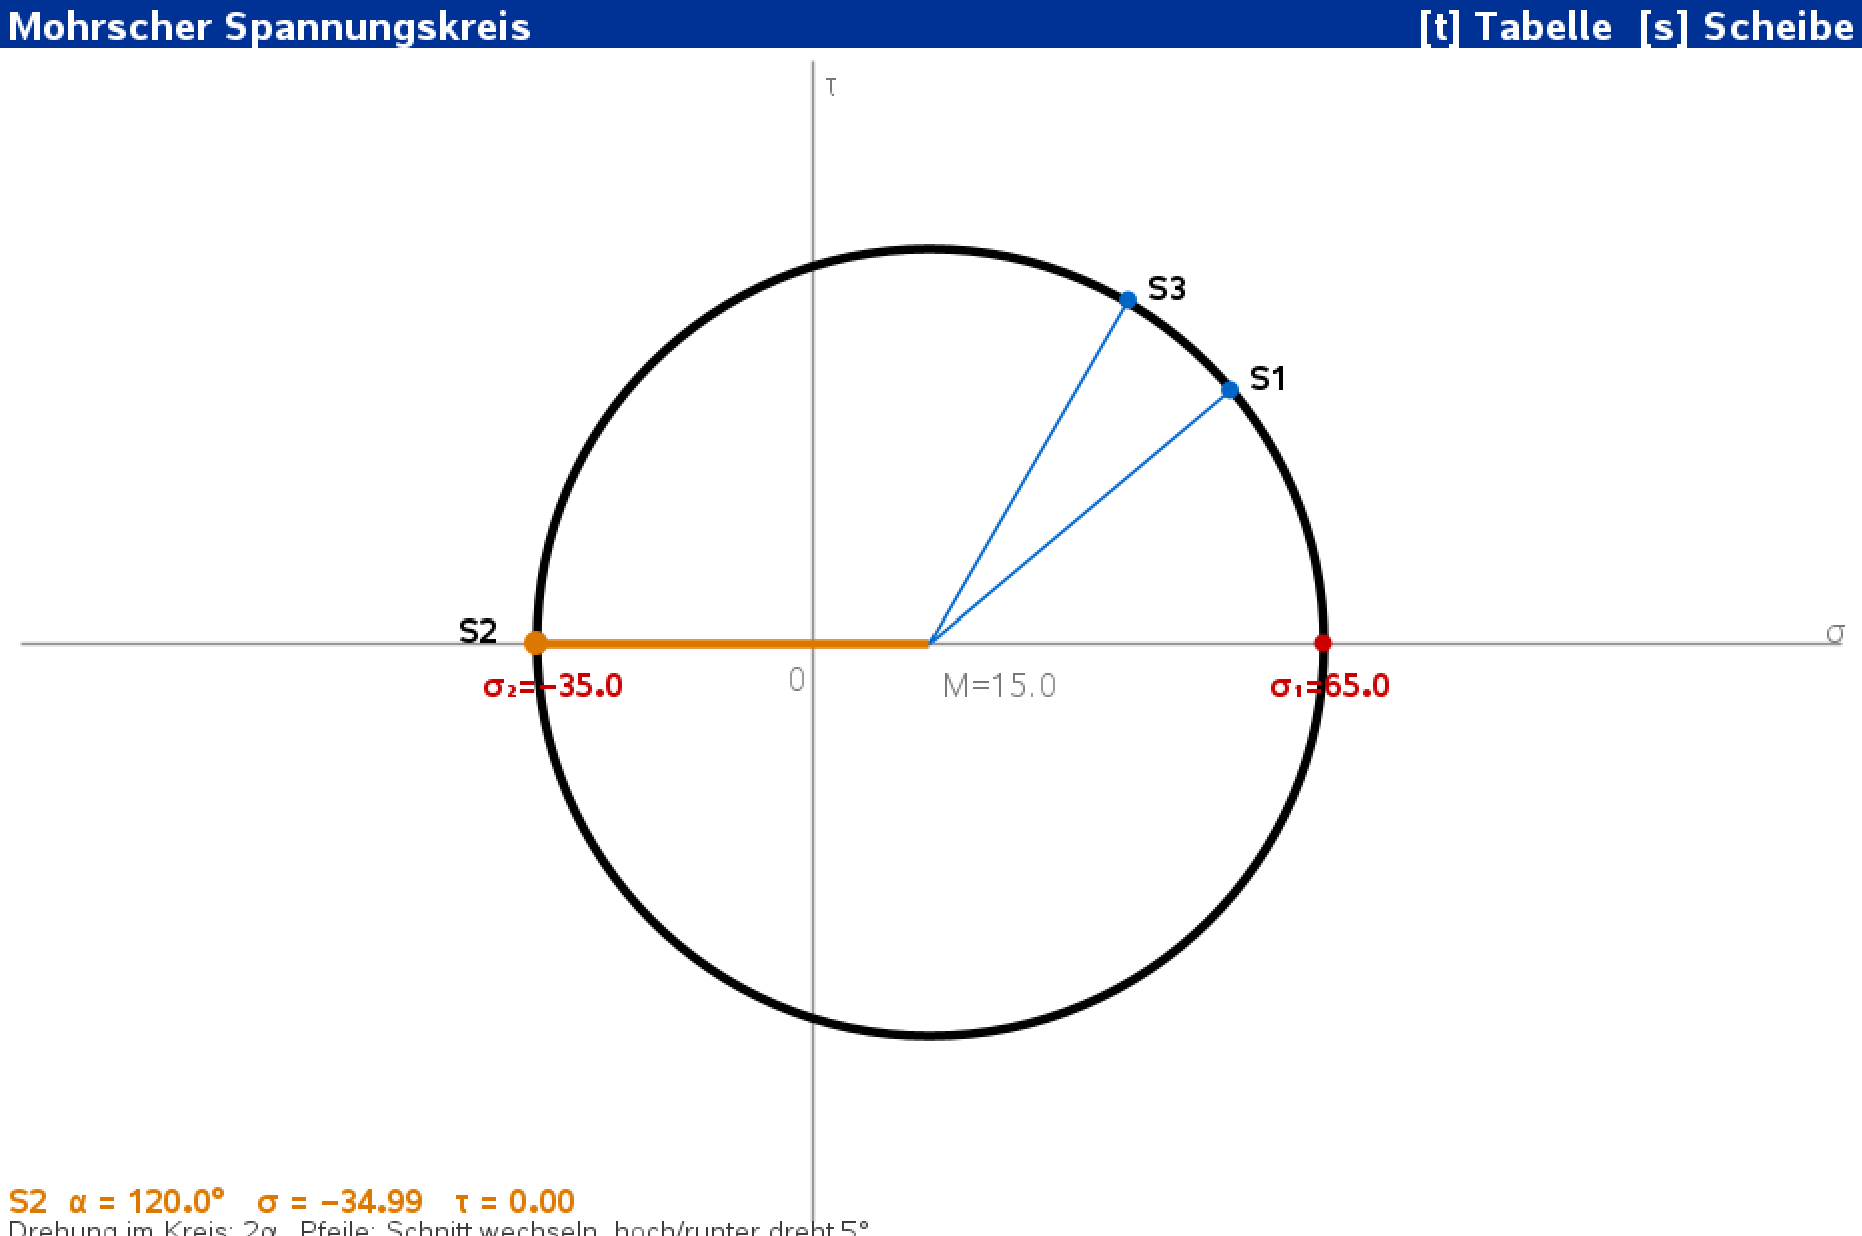
\includegraphics[width=\linewidth]{./fig/TM2/WiSe2122nr3_3.png}
        \caption{Spannungs-Kreis}
    \end{subfigure}
    \caption{Lösung von TM2 WiSe~21/22, Nr.~3}
    \label{fig:TM2WiSe2122Nr3_2}
\end{figure}

Falls bei einer Aufgabe nach dem Winkel eines Schnitts gefragt wird und das Programm zwei Winkel ausgibt, muss natürlich
geprüft werden, welcher Winkel eher zur Skizze passt.

\subsection{Schubspannung und SMP (TM2 SoSe 24 Nr.~8)}

\subsection{Verwölbung (TM2 SoSe 20 Nr.~9)} eingebunden.
% Hier keine \usepackage-Zeilen: Pakete stehen in der Praeambel von Anleitung.tex.
% Abbildungen mit [htbp]: LaTeX setzt sie dann dorthin, wo Platz ist. Im Text deshalb immer
% mit Abb.~\ref{...} auf sie verweisen, nicht mit "unten" oder "folgendermaßen".


\part{Beispiele}

In diesem Teil will ich anhand typischer Klausuraufgaben etwas genauer beschreiben, wie man das
Programm am besten verwendet, zumindest so, wie ich es für sinnvoll halte.

Die Screenshots habe ich in der PC-Ansicht gemacht, weil dort viele Dinge besser erkennbar sind.
Auf dem Taschenrechner selbst sollte mit Zoom aber auch alles erkennbar sein.

\section{TM1}
\subsection{WiSe~21/22}
\subsubsection{Geschlossenes System (Nr.~2)}
Bei dieser Aufgabe gibt es ein paar Besonderheiten bei der Eingabe, deshalb stelle ich sie hier vor.
Im Programm sieht das Tragwerk aus wie in Abb.~\ref{fig:WiSe2122nr2_1}.

\begin{figure}[htbp]
    \centering
    \begin{subfigure}[t]{0.48\textwidth}
        \centering
        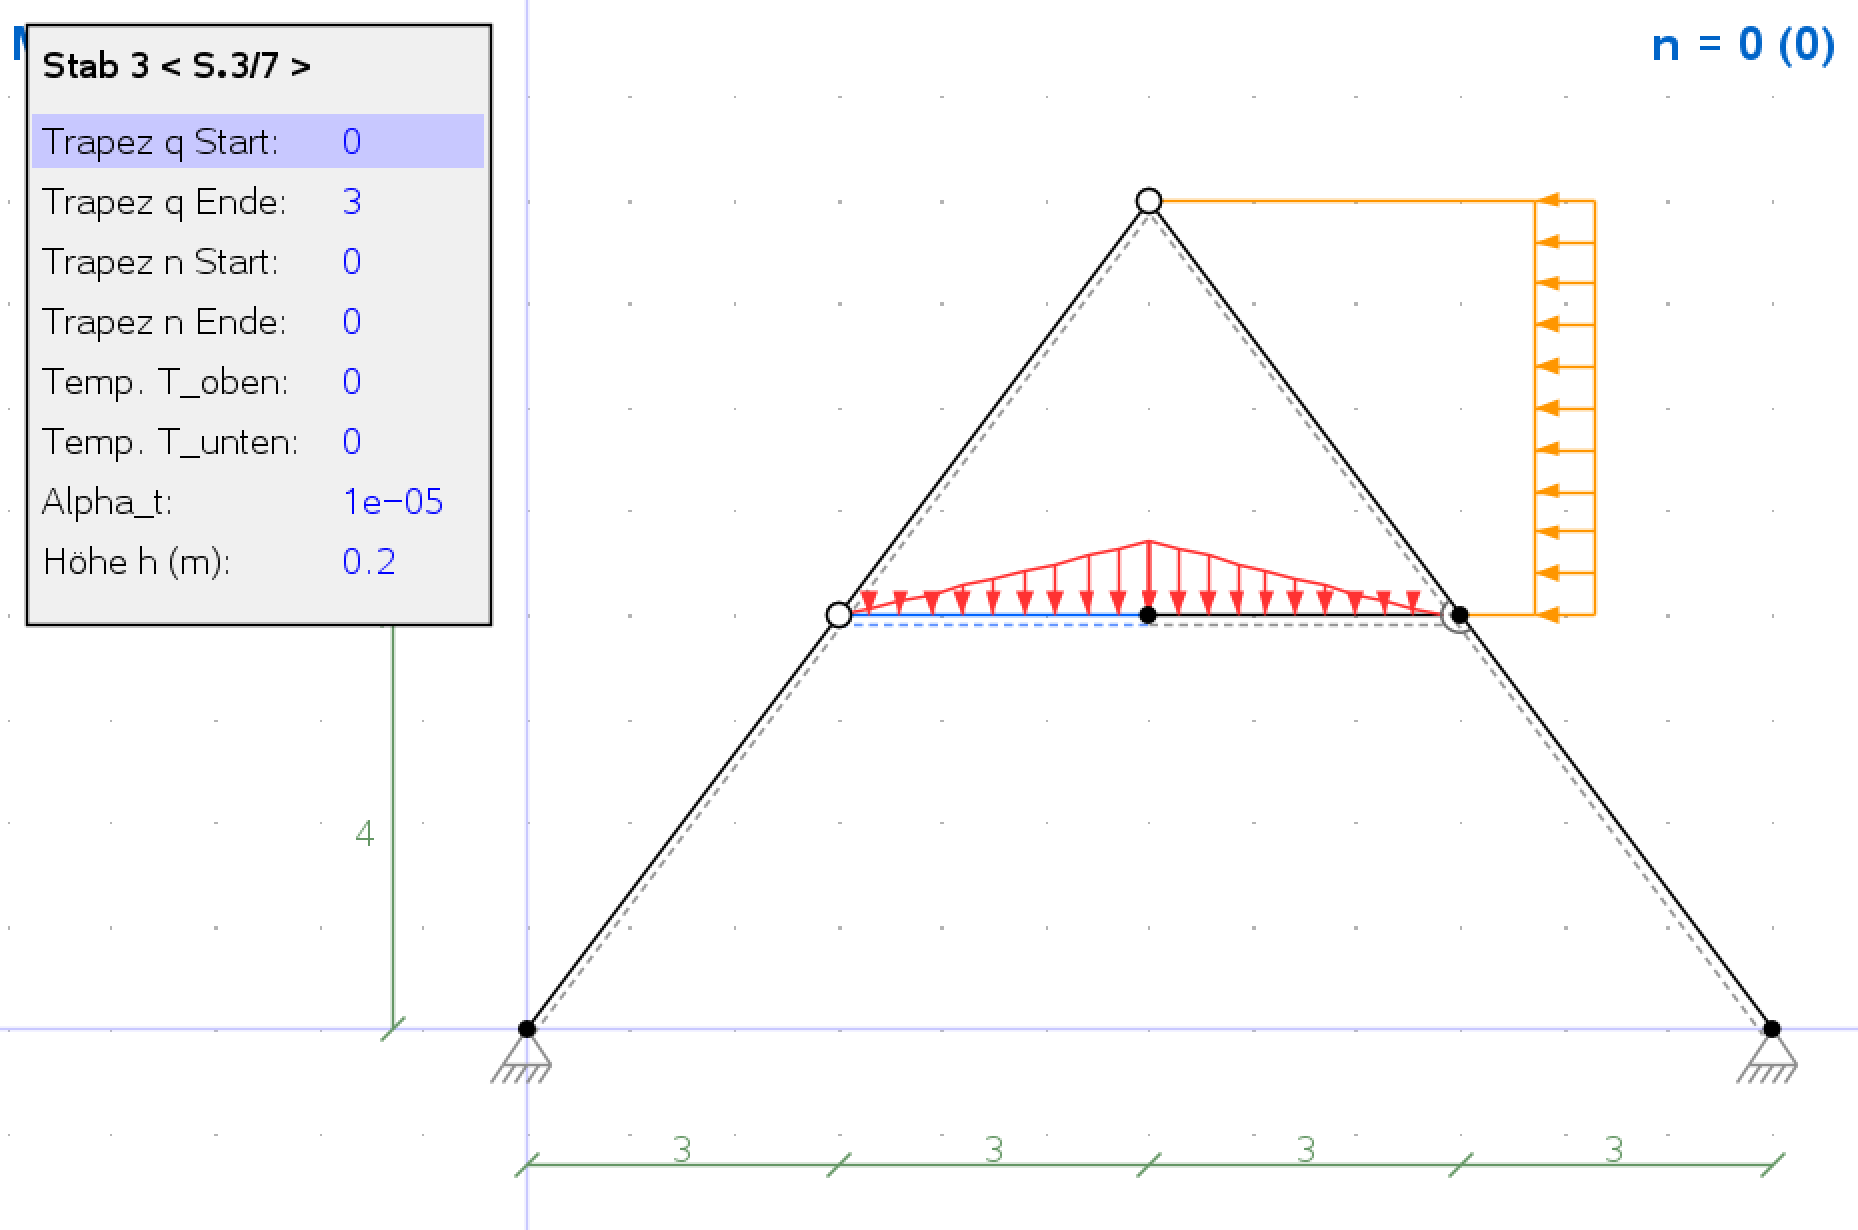
\includegraphics[width=\linewidth]{./fig/TM1/WiSe2122nr2_1.png}
        \caption{Trapezlast auf der linken Hälfte des Mittelstabs}
    \end{subfigure}
    \hfill
    \begin{subfigure}[t]{0.48\textwidth}
        \centering
        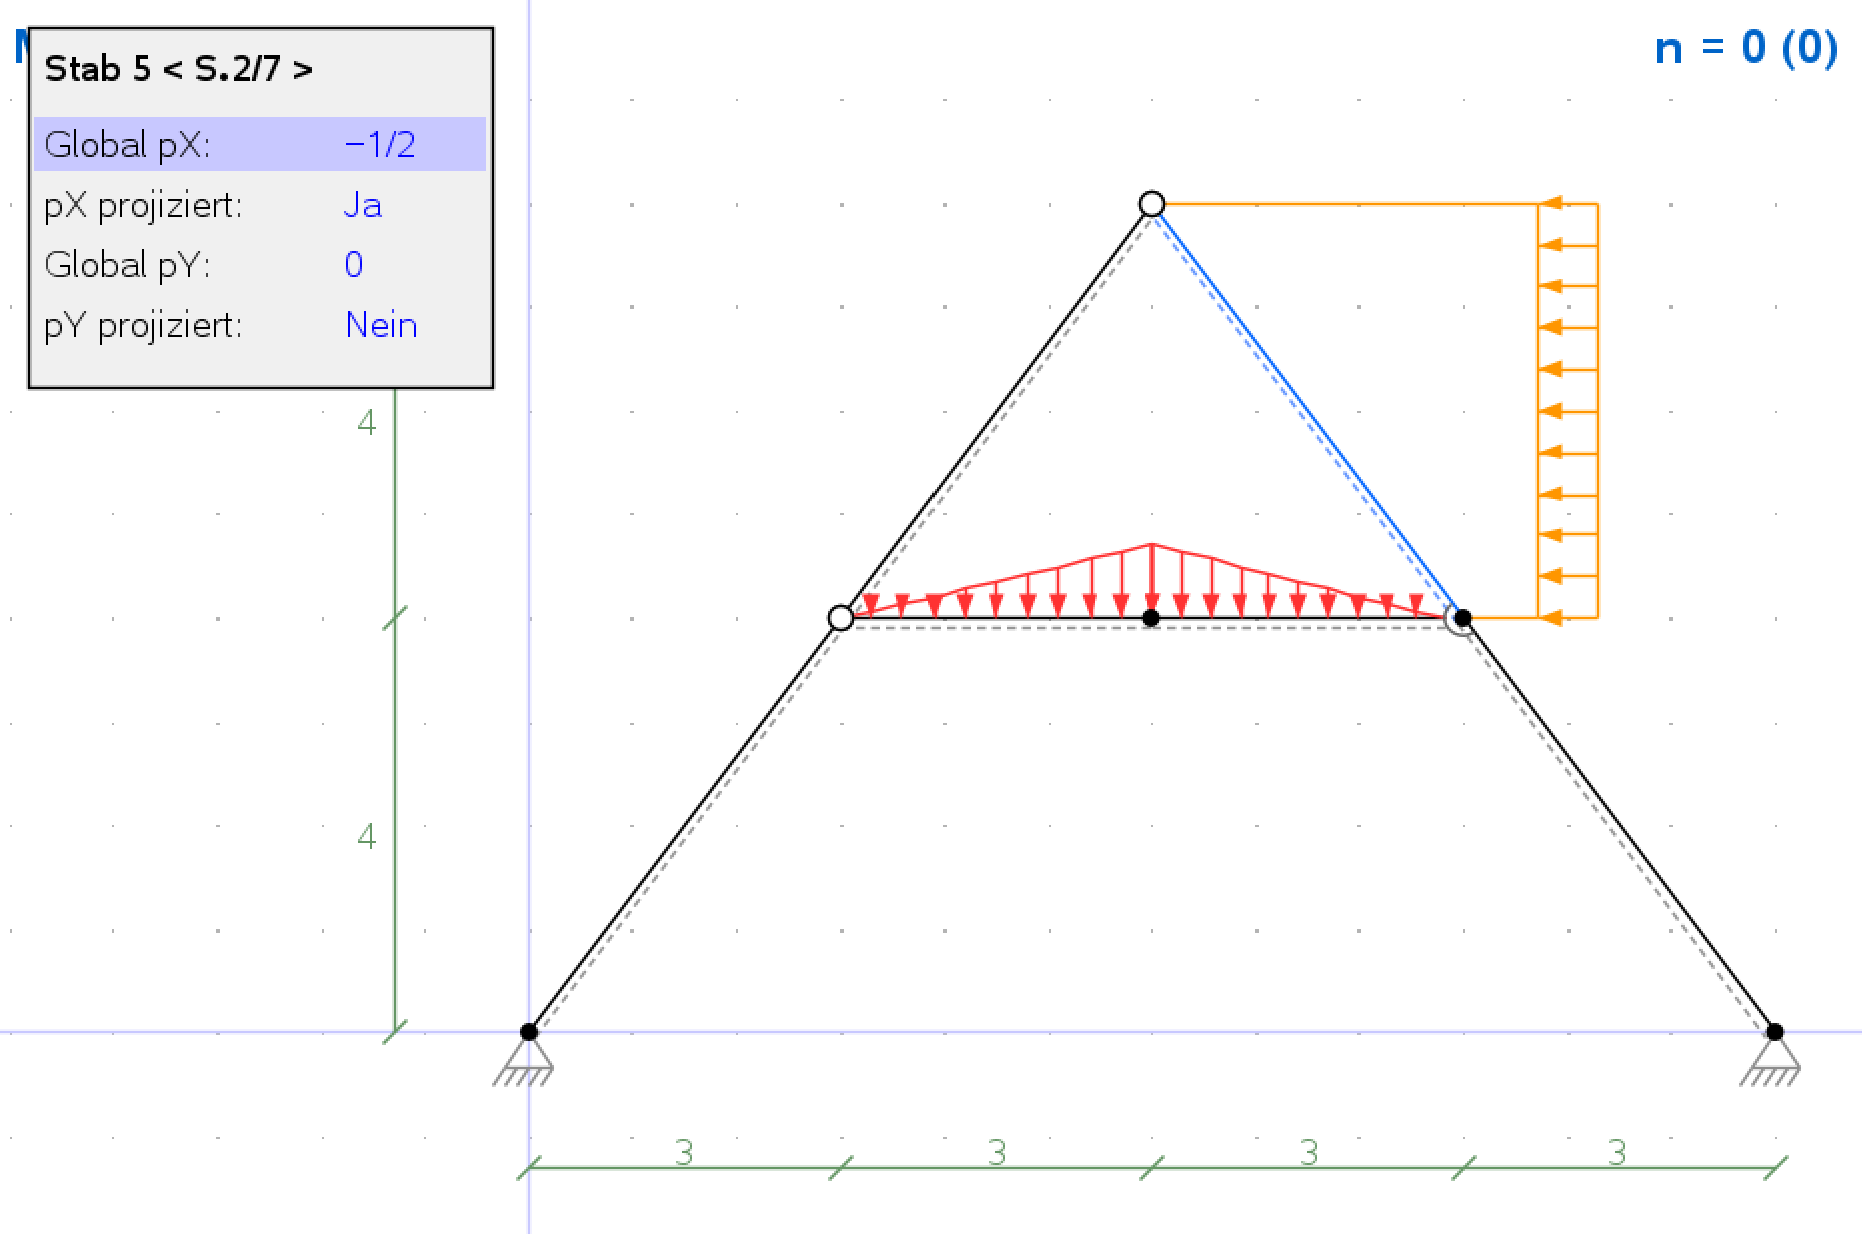
\includegraphics[width=\linewidth]{./fig/TM1/WiSe2122nr2_2.png}
        \caption{globale Streckenlast am oberen rechten Stab}
    \end{subfigure}
    \caption{WiSe~21/22, Nr.~2 im Programm}
    \label{fig:WiSe2122nr2_1}
\end{figure}

Den Stab in der Mitte müsst ihr im Programm teilen. Die Last auf ihm ist dreieckförmig mit der
Spitze in der Mitte, eine Trapezlast geht aber immer über einen ganzen Stab. Jede Hälfte bekommt
deshalb ihre eigene Trapezlast, die linke von $0$ auf $3$, die rechte von $3$ auf $0$
(Abb.~\ref{fig:WiSe2122nr2_1}a). Der neue Knoten in der Mitte bleibt biegesteif.

Die Streckenlast am schrägen Stab gebt ihr am einfachsten als globale Last ein
(Abb.~\ref{fig:WiSe2122nr2_1}b). In der Aufgabe ist sie auf die senkrechte Projektion des Stabes
bezogen, deshalb muss \emph{pX projiziert} auf \emph{Ja} stehen. Negativ ist sie, weil sie global
gesehen entgegen der $x$-Achse wirkt, also nach links.

Nach dem Berechnen könnt ihr das LGS, das zur Explosionsansicht (Abb.~\ref{fig:WiSe2122nr2_2})
gehört, über die zweite Seite des Obermenüs (\emph{LGS-Matrix}) in den Taschenrechner exportieren
(Abb.~\ref{fig:WiSe2122nr2_3}). Die Gleichungen stehen dann lesbar in \code{lgs}, die Lösung
bekommt ihr zum Beispiel mit \code{ggw\_x = ggw\_a$^{-1}$*ggw\_b}
(Abschnitt~\ref{sec:lgs-matrix}).

\begin{figure}[htbp]
    \centering
    \begin{subfigure}[t]{0.48\textwidth}
        \centering
        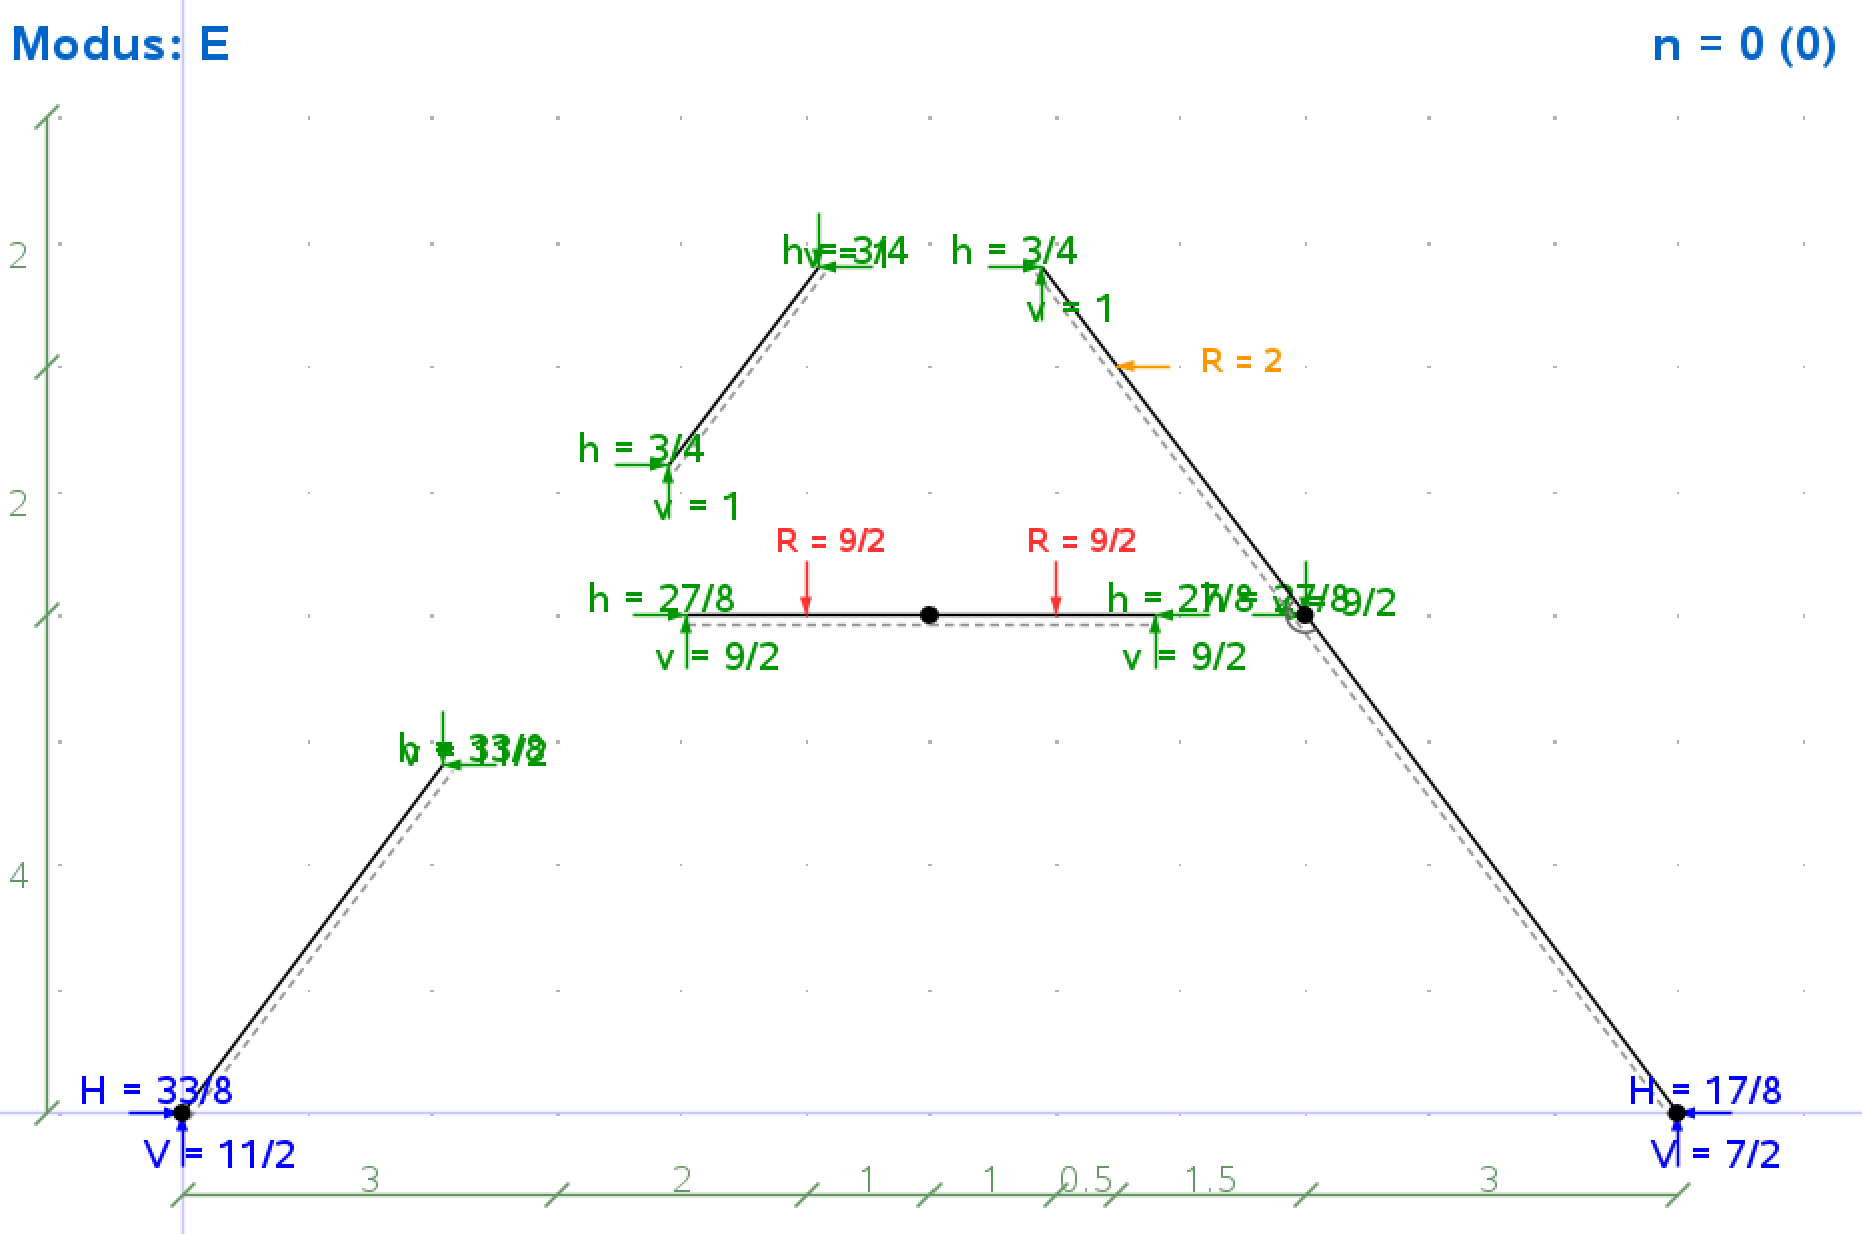
\includegraphics[width=\linewidth]{./fig/TM1/WiSe2122nr2_5.png}
        \caption{Seite~1: Ergebnisse in ihrer wirklichen Richtung}
    \end{subfigure}
    \hfill
    \begin{subfigure}[t]{0.48\textwidth}
        \centering
        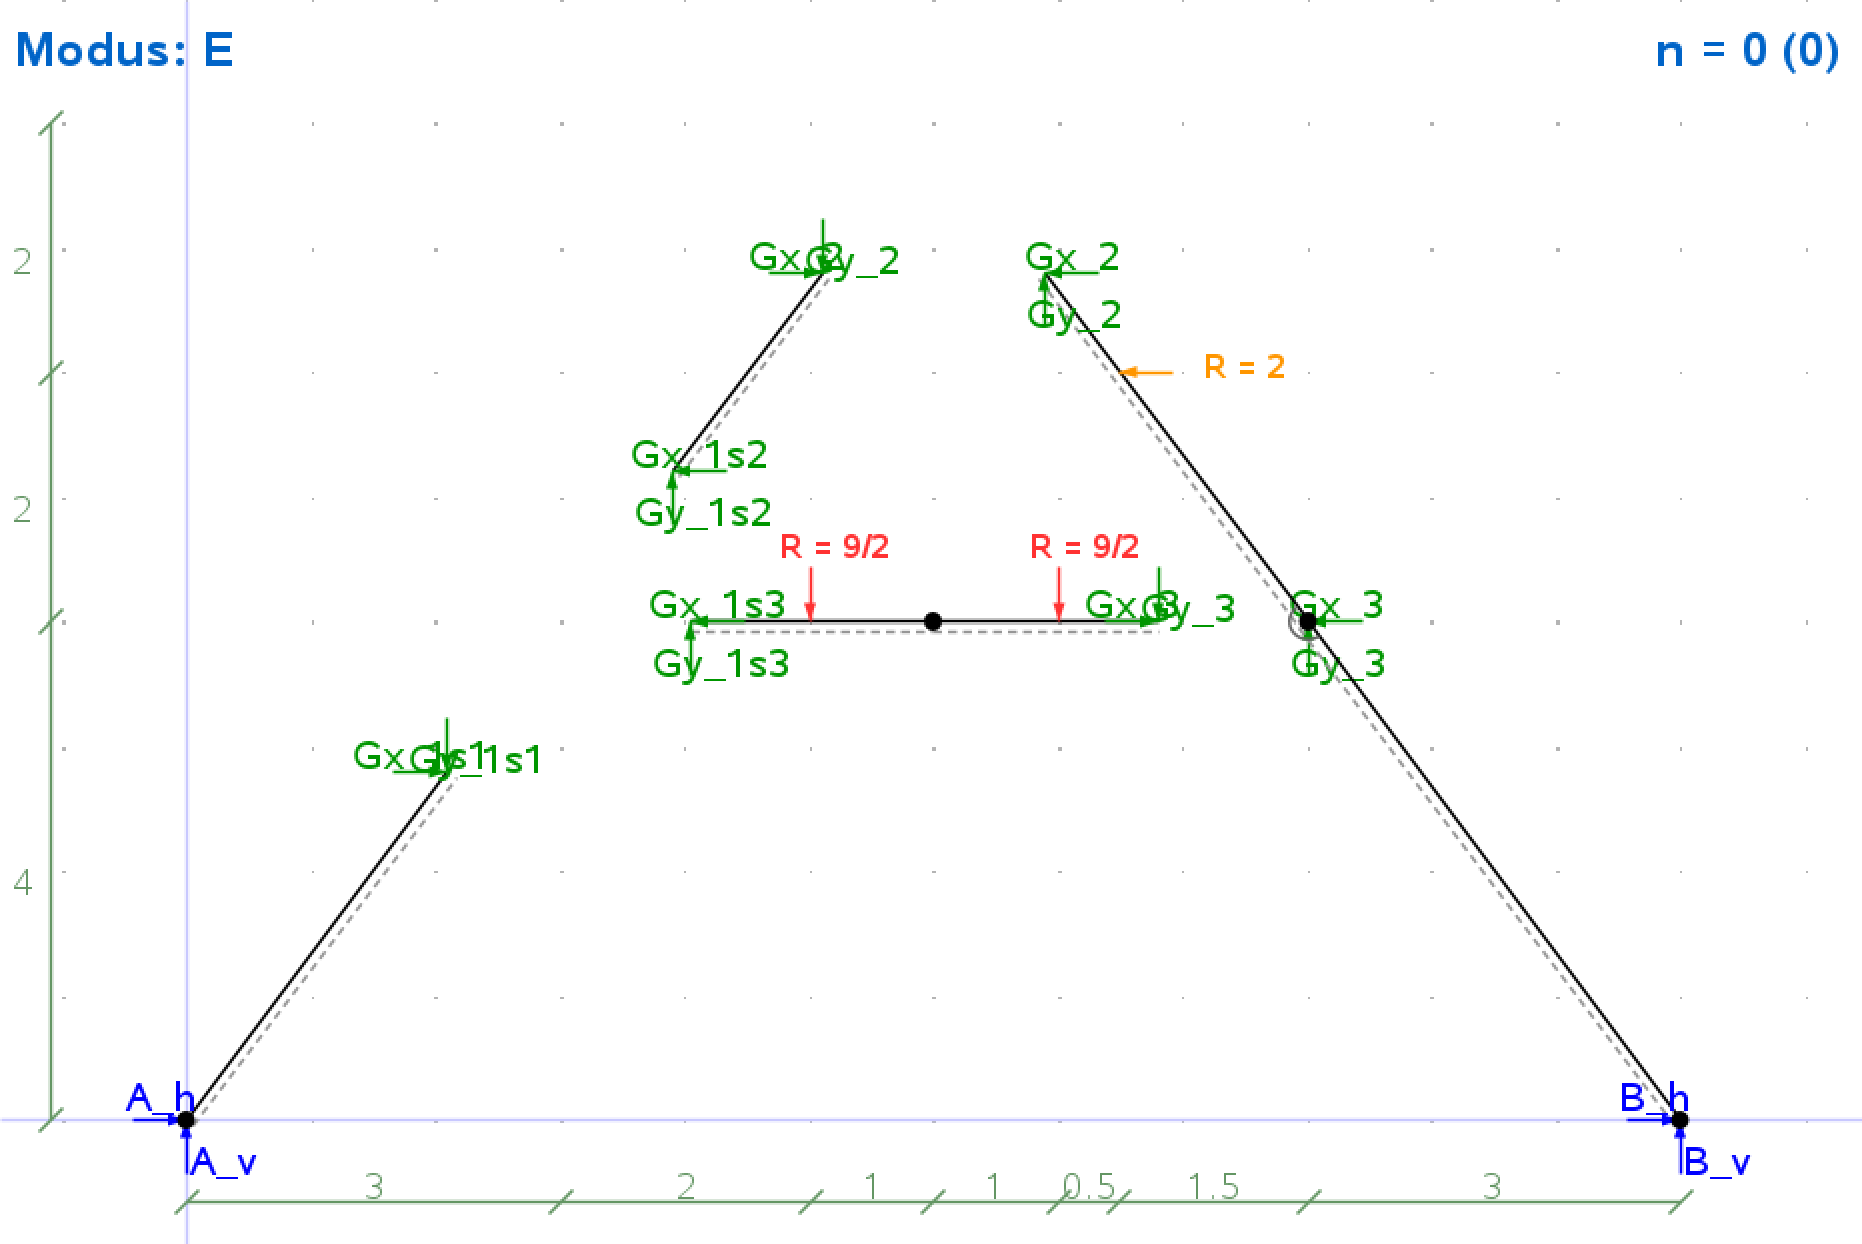
\includegraphics[width=\linewidth]{./fig/TM1/WiSe2122nr2_6.png}
        \caption{Seite~2: Unbekannte in positiver Richtung}
    \end{subfigure}
    \caption{WiSe~21/22, Nr.~2: Explosionsansicht (E-Modus)}
    \label{fig:WiSe2122nr2_2}
\end{figure}

\begin{figure}[htbp]
    \centering
    \begin{subfigure}[t]{0.48\textwidth}
        \centering
        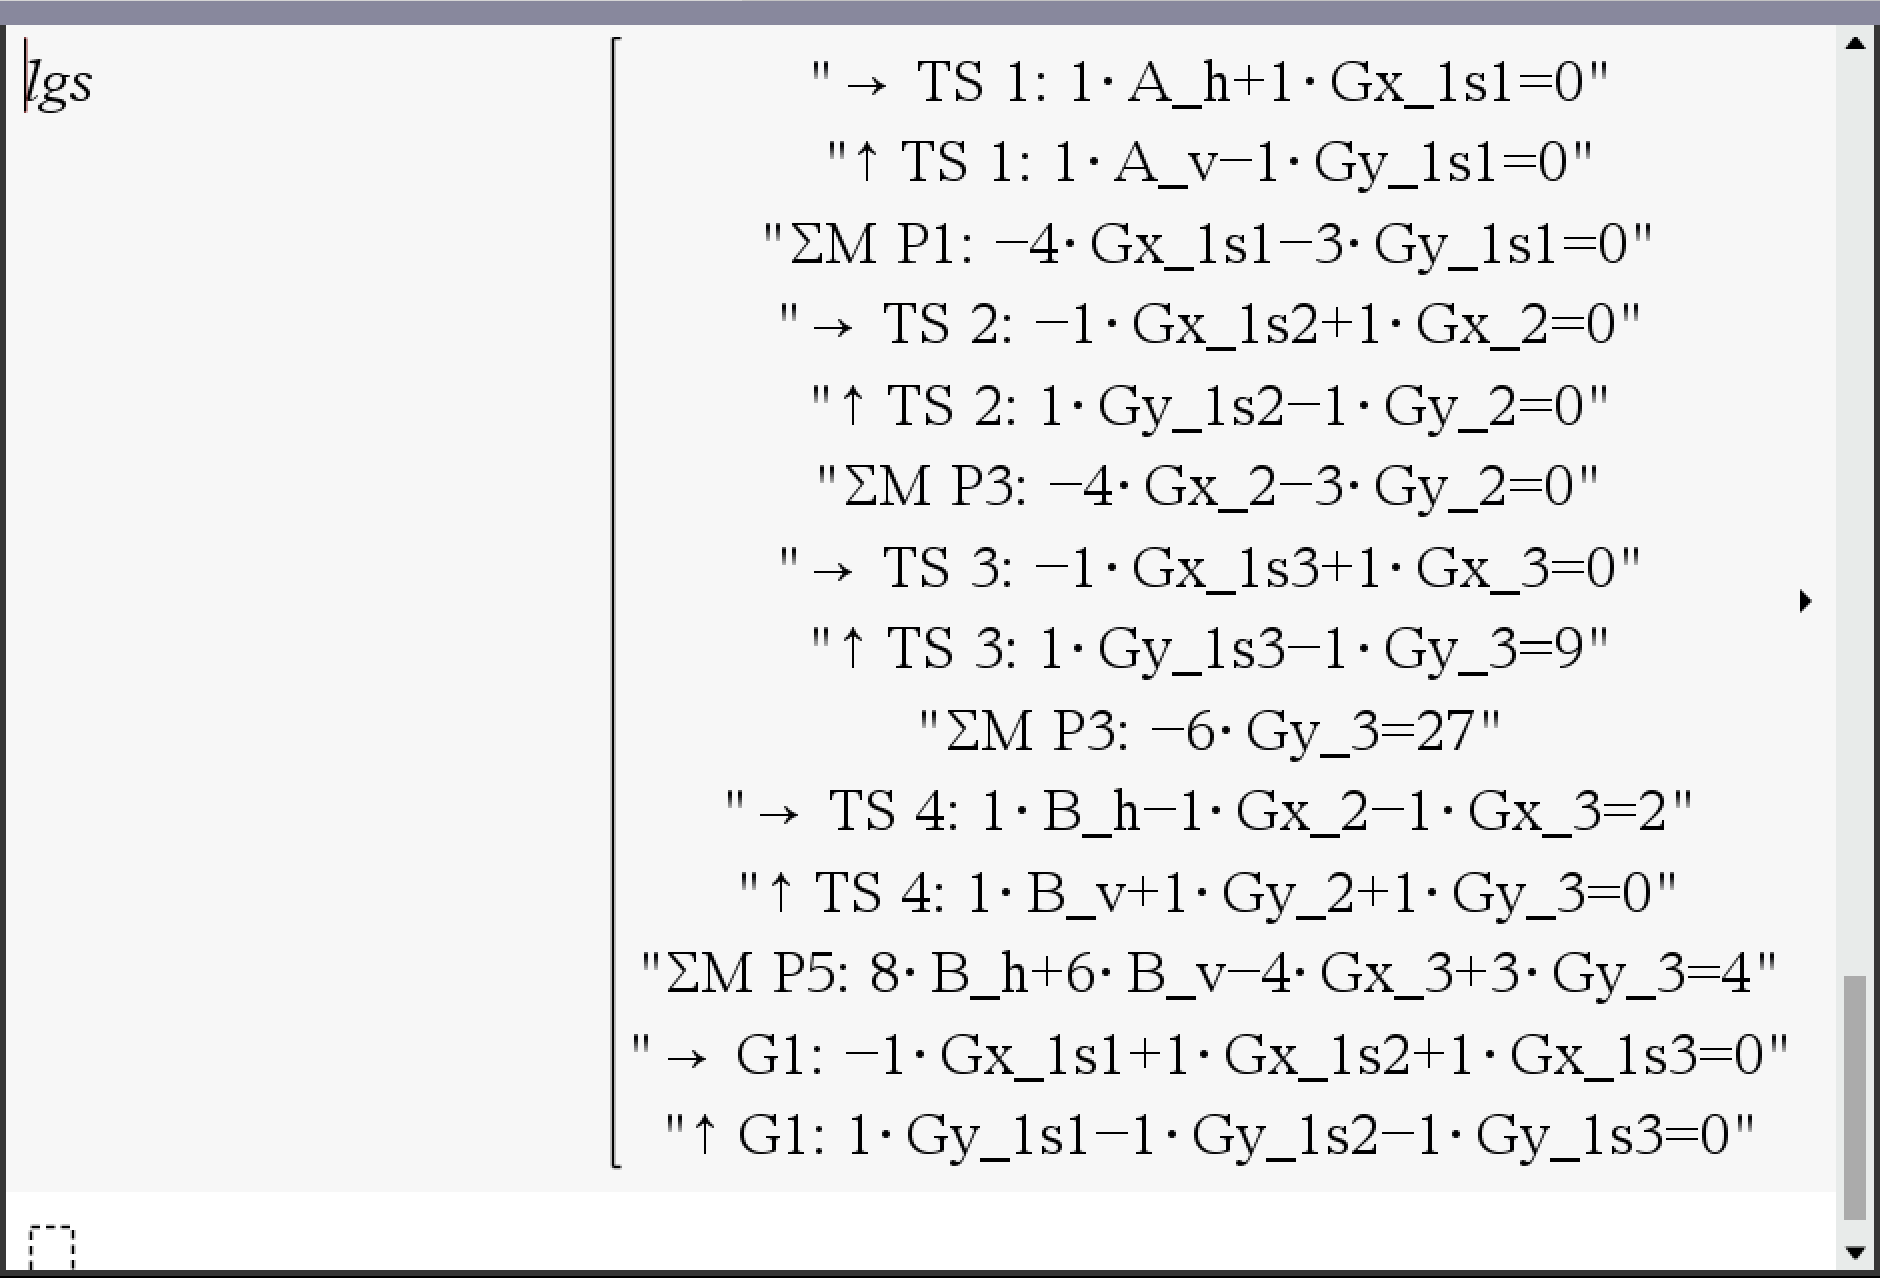
\includegraphics[width=\linewidth]{./fig/TM1/WiSe2122nr2_3.png}
        \caption{exportierte Gleichungen \code{lgs}}
    \end{subfigure}
    \hfill
    \begin{subfigure}[t]{0.48\textwidth}
        \centering
        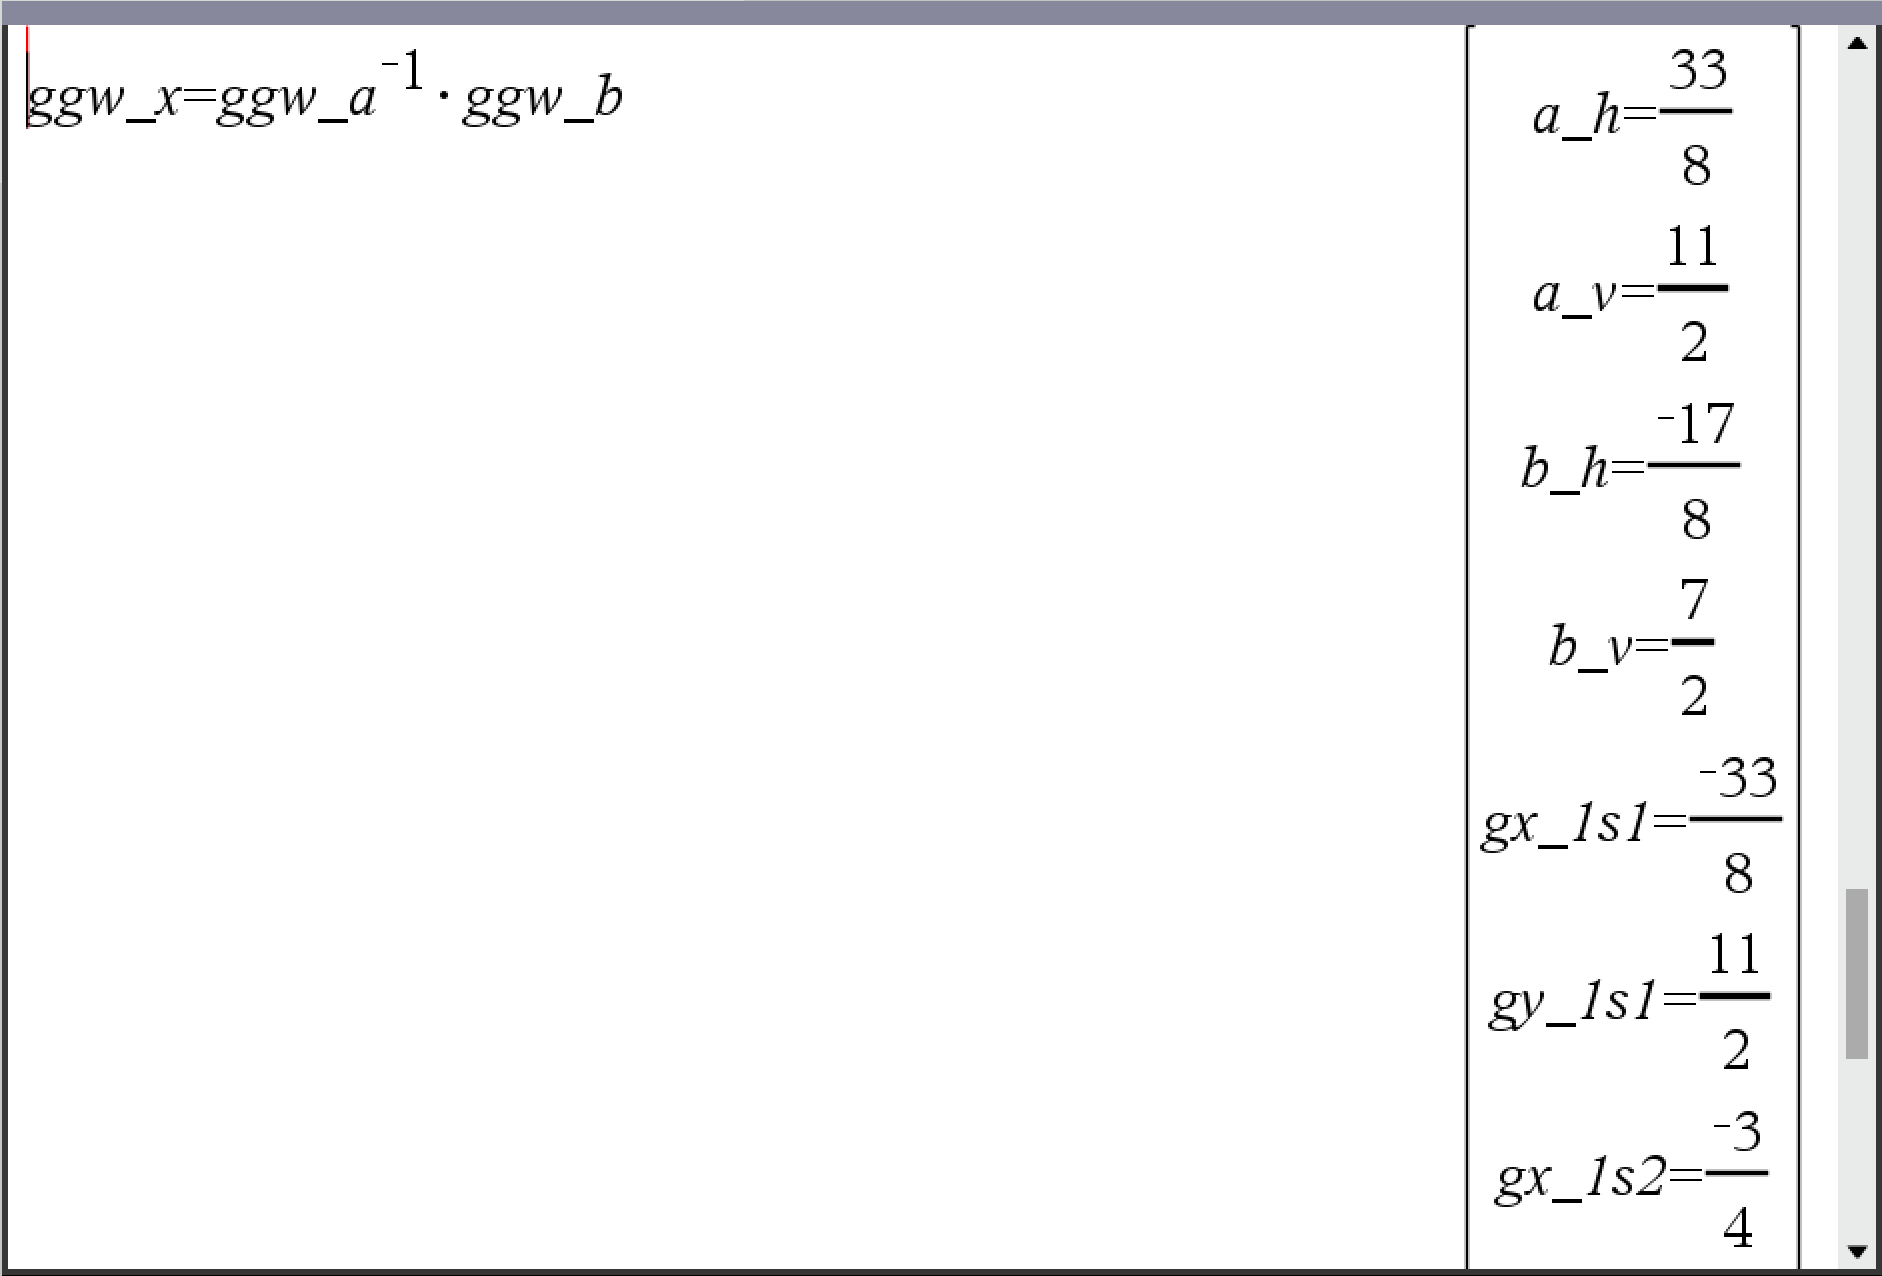
\includegraphics[width=\linewidth]{./fig/TM1/WiSe2122mr2_4.png}
        \caption{Lösung mit \code{ggw\_x}}
    \end{subfigure}
    \caption{WiSe~21/22, Nr.~2: exportiertes LGS}
    \label{fig:WiSe2122nr2_3}
\end{figure}

Die Explosionsansicht kann manchmal etwas unübersichtlich sein. Wenn ihr nah genug heranzoomt,
sollte aber trotzdem alles erkennbar sein. Die Ergebnisse müsst ihr natürlich nicht in dieser
Vektorform aufschreiben, nur ihr Inhalt zählt.

An dieser Stelle will ich anmerken, dass meist nur bei Systemen mit einem geschlossenen Ring wie
diesem nach allen Gelenk- und Auflagerkräften gefragt wird. Bei offenen Systemen ohne Ring wird oft
nur nach den Auflagerkräften gefragt. Das exportierte LGS liefert dann zwar auch die richtige Lösung, ist aber
meist mehr, als ihr braucht. Den Punkt, um den das Programm die Momentensumme eines Teilsystems
bildet, seht ihr, wenn ihr in der Explosionsansicht mit der Maus über das Teilsystem fahrt
(\emph{Hover}).

Die Zustandslinien, also die Verläufe der Schnittgrößen, zeichnet euch das Programm mit den Tasten
\taste{n}, \taste{q} und \taste{m}, die könnt ihr einfach abzeichnen. Falls ihr Randwerte schlecht
erkennt, fahrt mit der Maus über den jeweiligen Stab, dann zeigt das Programm nur noch diesen Stab
mit seinen Randwerten an.

\subsubsection{Qualitavtive Verläufe im symbolischen Modus (Nr.~4)}

Um meinen den oben genannten Punkt zum symbolischen Modus zu verdeutlichen will ich hier kurz auf Teilaufgabe b) eingehen.
Das System und der Querkraftverlauf sind in Abbildung~\ref{fig:TM1WiSe2122Nr4} dargestellt.

\begin{figure}[htbp]
    \centering
    \begin{subfigure}[t]{0.48\textwidth}
        \centering
        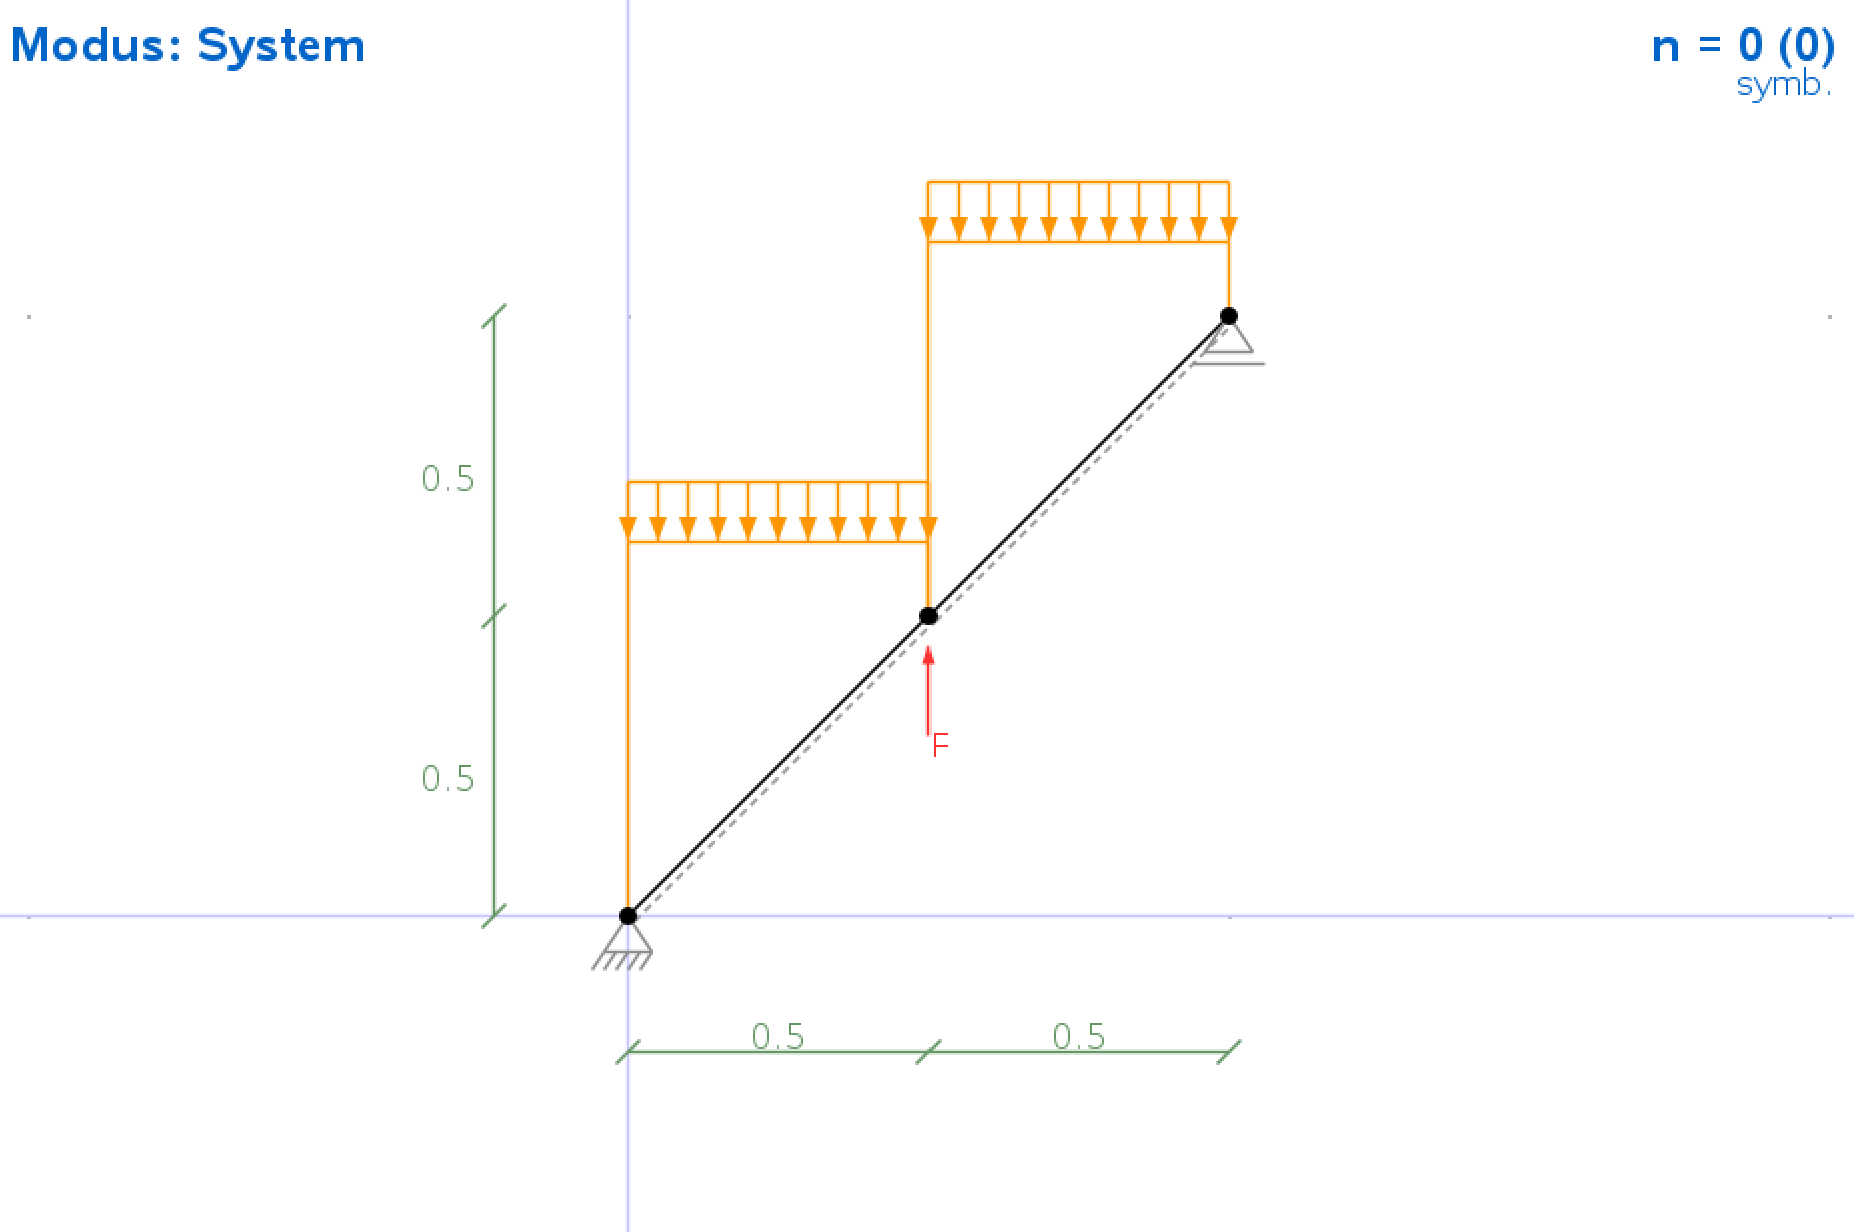
\includegraphics[width=\linewidth]{./fig/TM1/WiSe2122nr4_1.png}
        \caption{System}
    \end{subfigure}
    \hfill
    \begin{subfigure}[t]{0.48\textwidth}
        \centering
        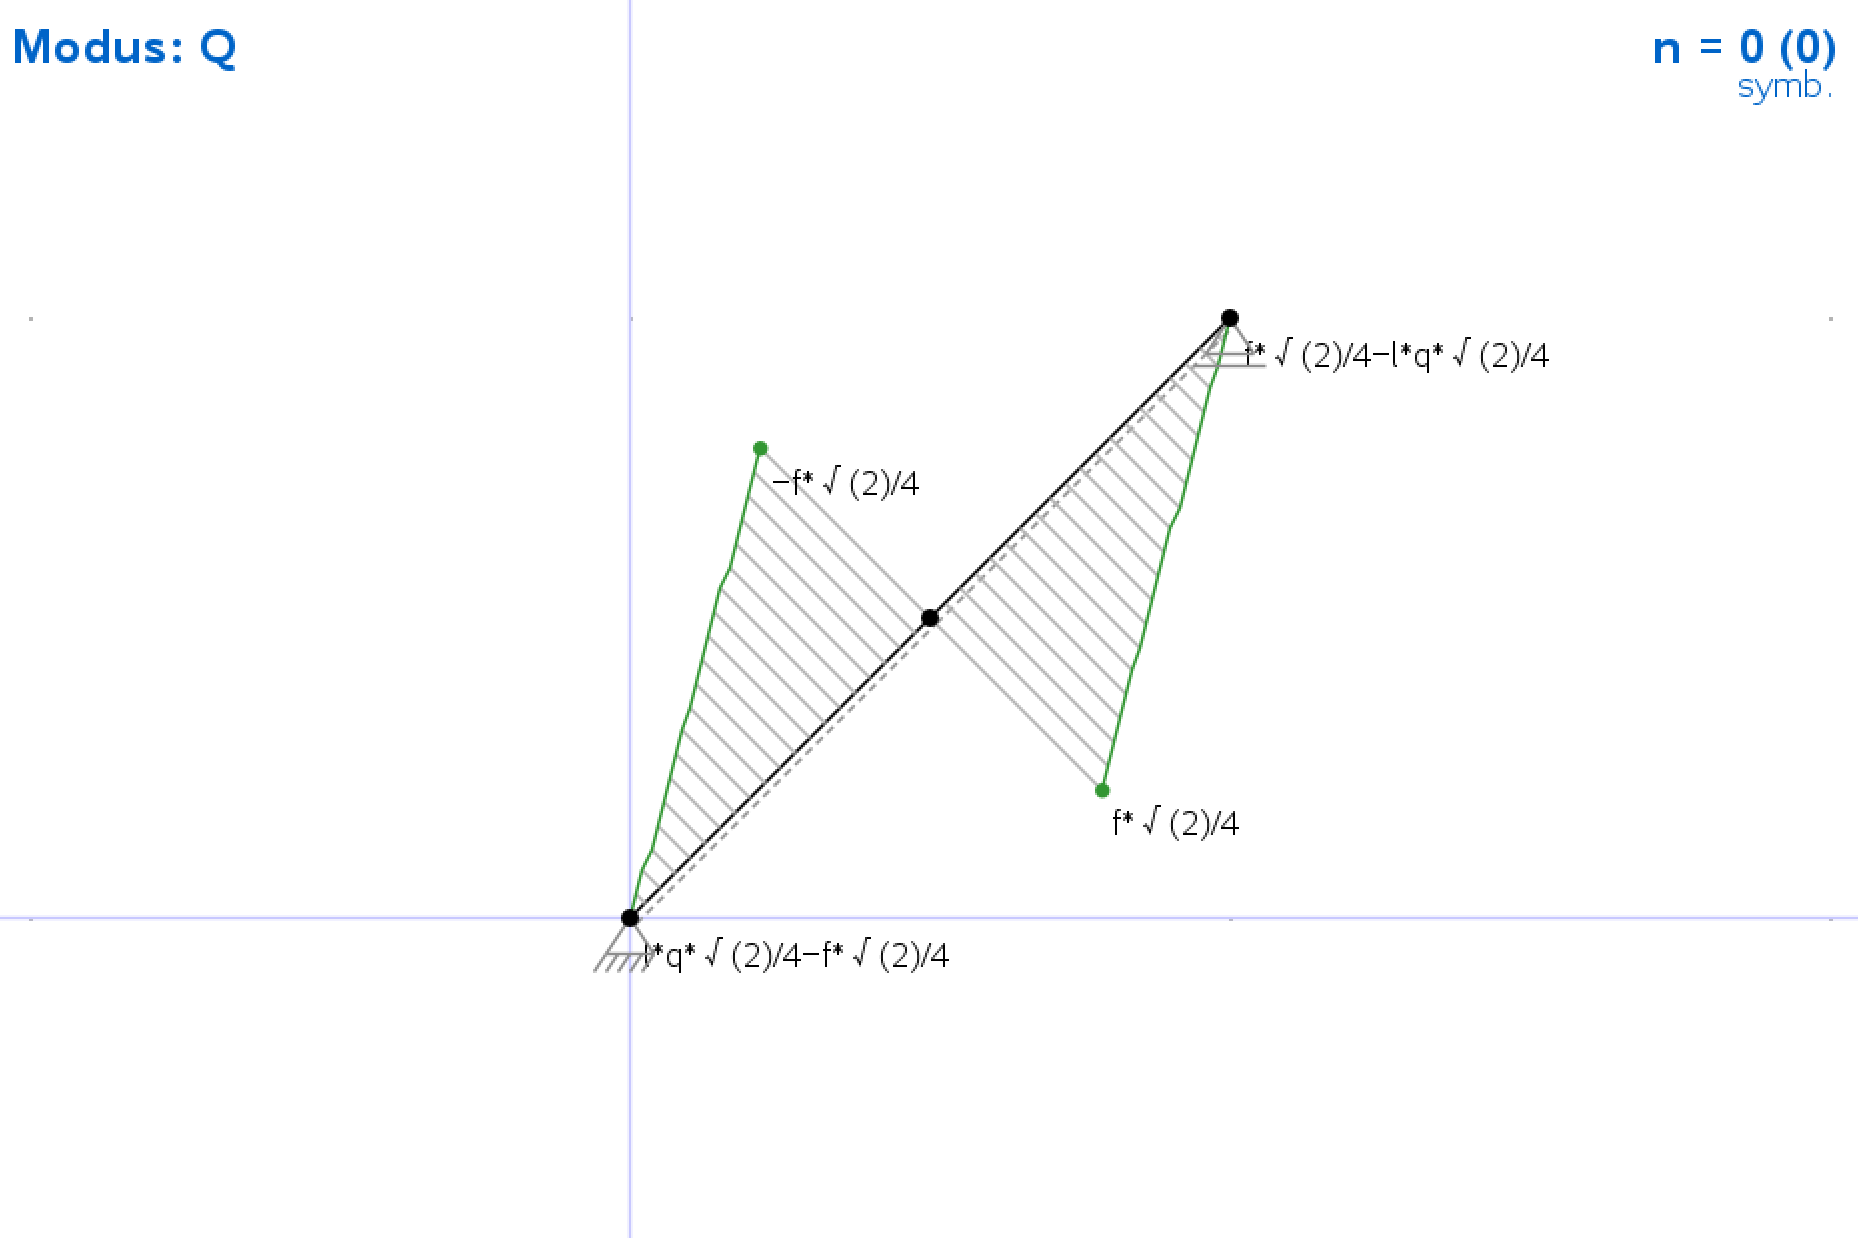
\includegraphics[width=\linewidth]{./fig/TM1/WiSe2122nr4_2.png}
        \caption{Querkraftverlauf}
    \end{subfigure}
    \caption{WiSe~21/22, Nr.~4}
    \label{fig:TM1WiSe2122Nr4}
\end{figure}

Im Querkraft verlauf sieht es so aus, als ob diese an den Auflagern null wird. Wenn man sich die Beschriftung der Randwerte 
anschaut wird jedoch klar, dass ist nur der Fall, wenn $q\cdot l=F$ bzw. $q\cdot a=F$ gilt. Das ist eben genau die Annhame des Programms,
um überhaupt irgendeinen Verlauf zeichnen zu können.
Die Aufgabe gibt aber unten vor: $F>q\cdot a$. Damit wird die Qerkraft am linekn Ende negativ und am rechten Ende positiv.
Die Verläufe von symbolische Berechnungen solltet ihr also \textbf{nie} einfach blind abzeichnen.

\subsection{PvV (Nr.~3)}

Zum PvV gibt es eigentlich nicht viel zu sagen. System zeichnen, \taste{v} drücken, Bindung wählen, abzeichnen,
dann exportieren und aufschreiben. 


\begin{figure}[htbp]
    \centering
    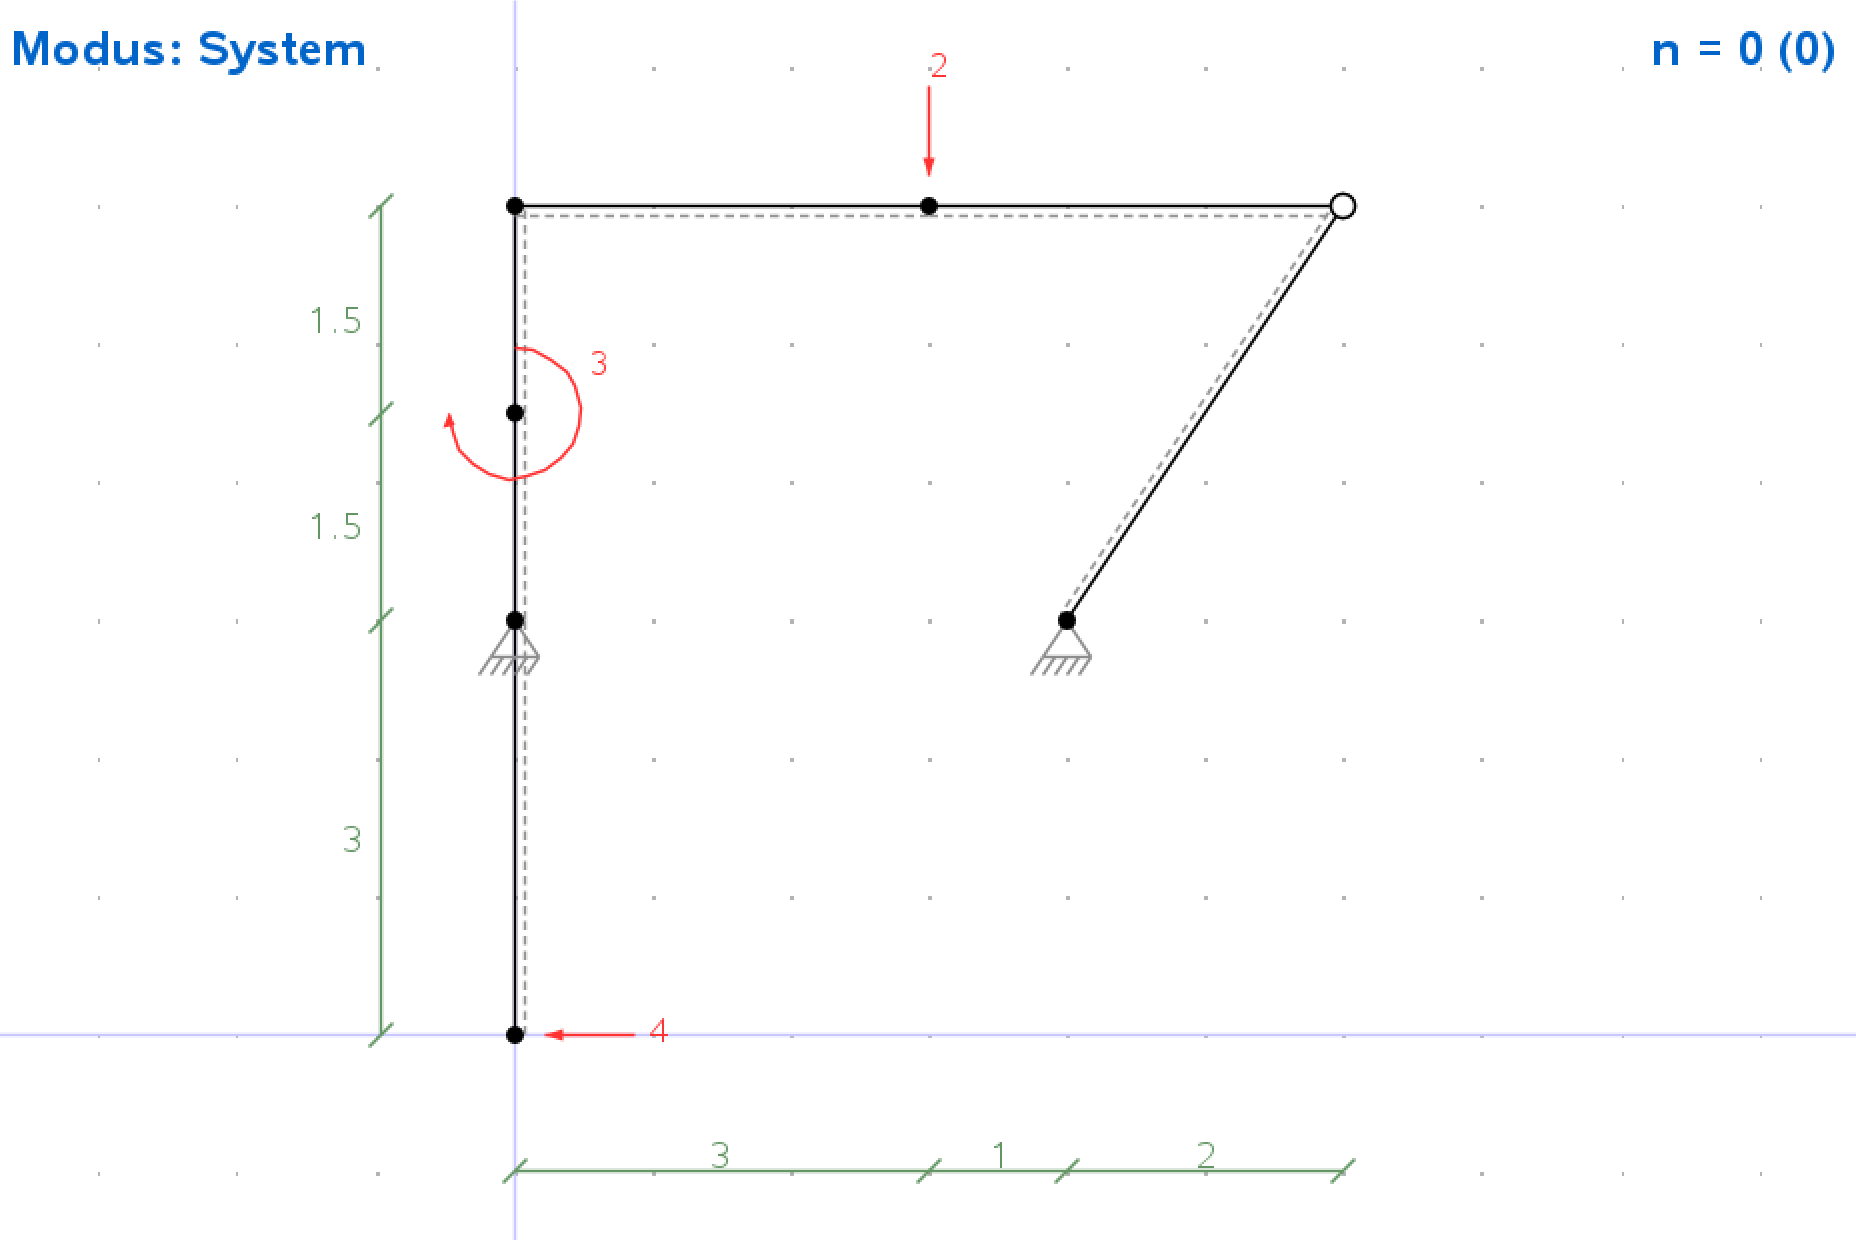
\includegraphics[width=0.5\linewidth]{./fig/TM1/WiSe2122nr3_1.png}
    \caption{TM1 WiSe~21/22, Nr.~3 im Programm}
    \label{fig:TM1WiSe2122Nr3_1}
\end{figure}

\begin{figure}[htbp]
    \centering
    \begin{subfigure}[t]{0.48\textwidth}
        \centering
        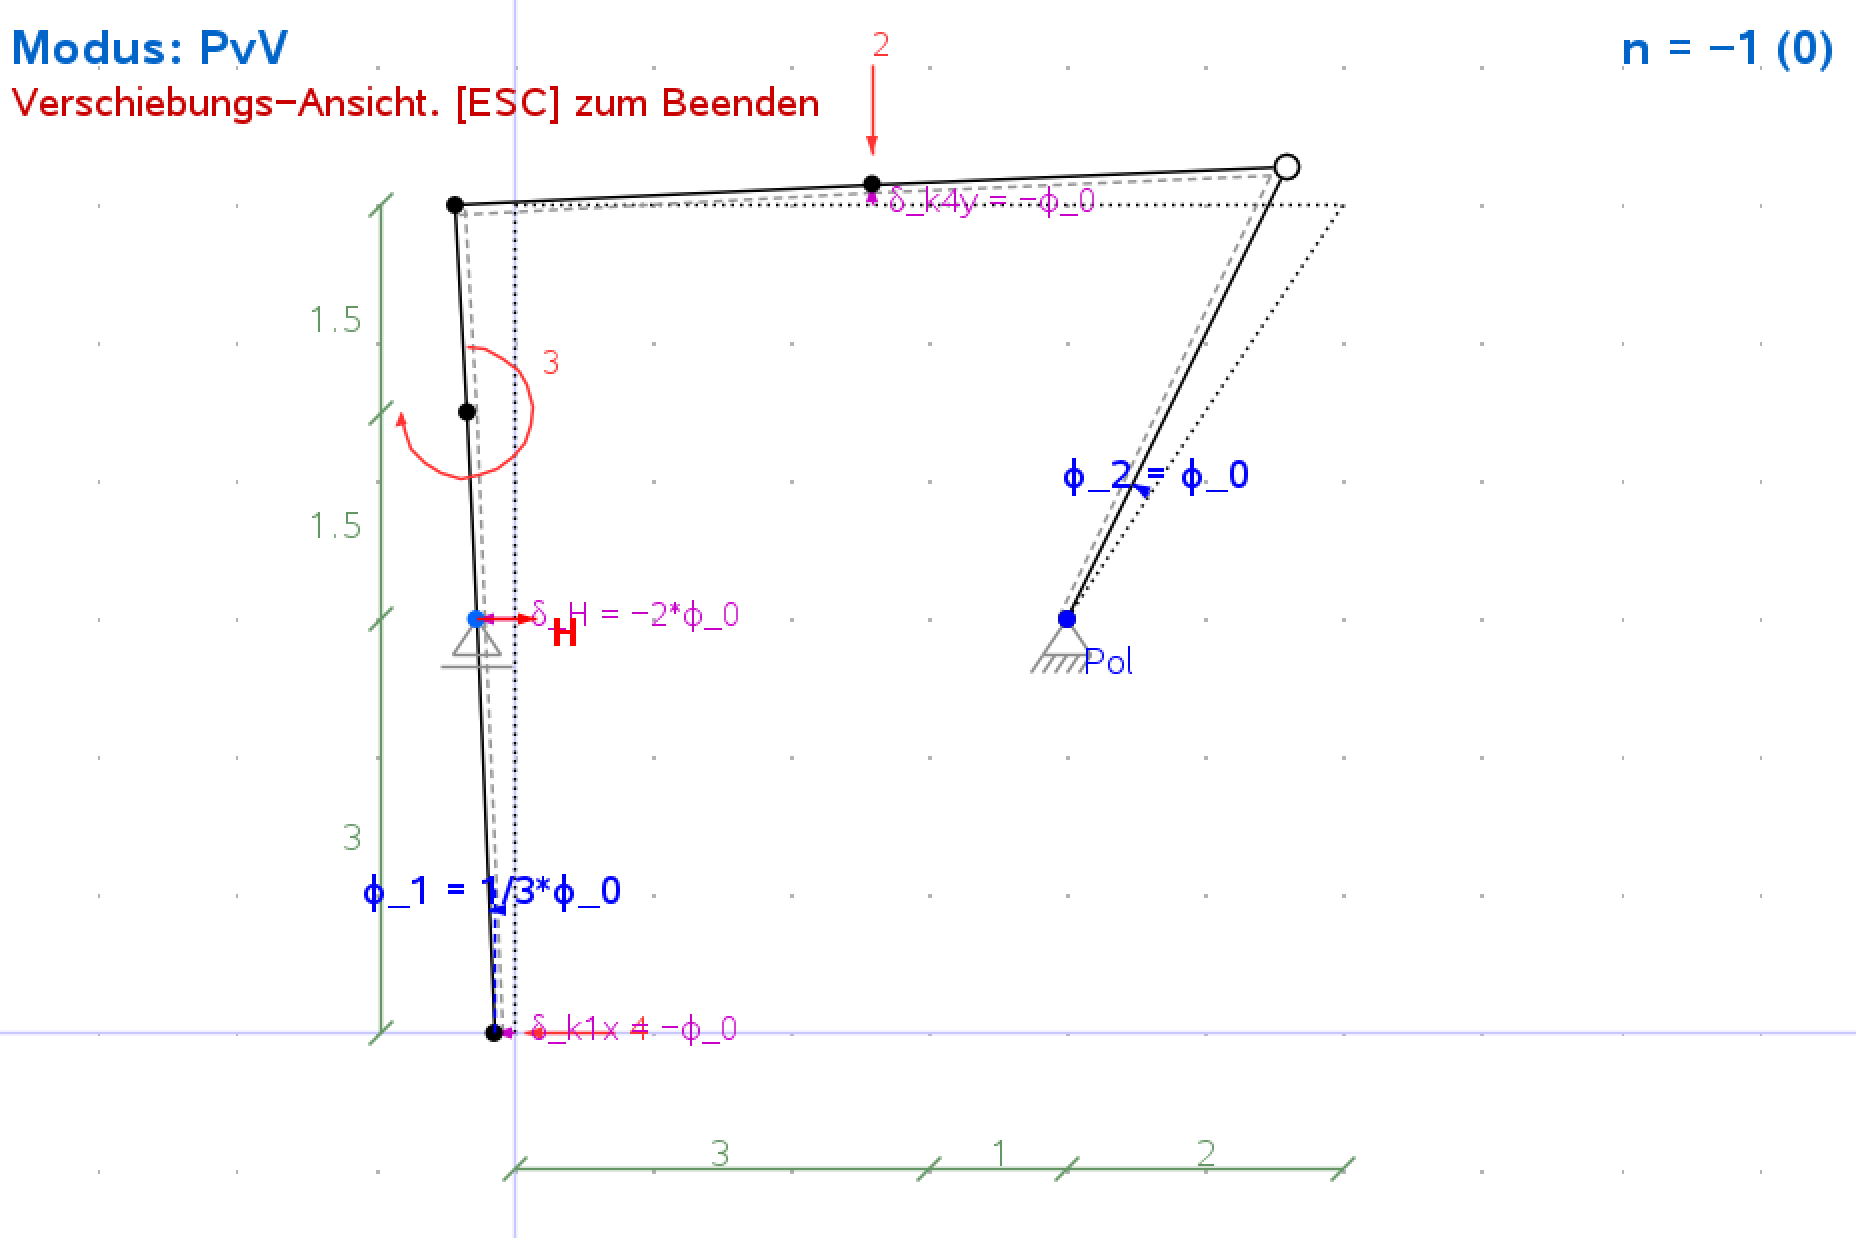
\includegraphics[width=\linewidth]{./fig/TM1/WiSe2122nr3_2.png}
        \caption{Verschiebungsfigur für $A_H$}
    \end{subfigure}
    \hfill
    \begin{subfigure}[t]{0.48\textwidth}
        \centering
        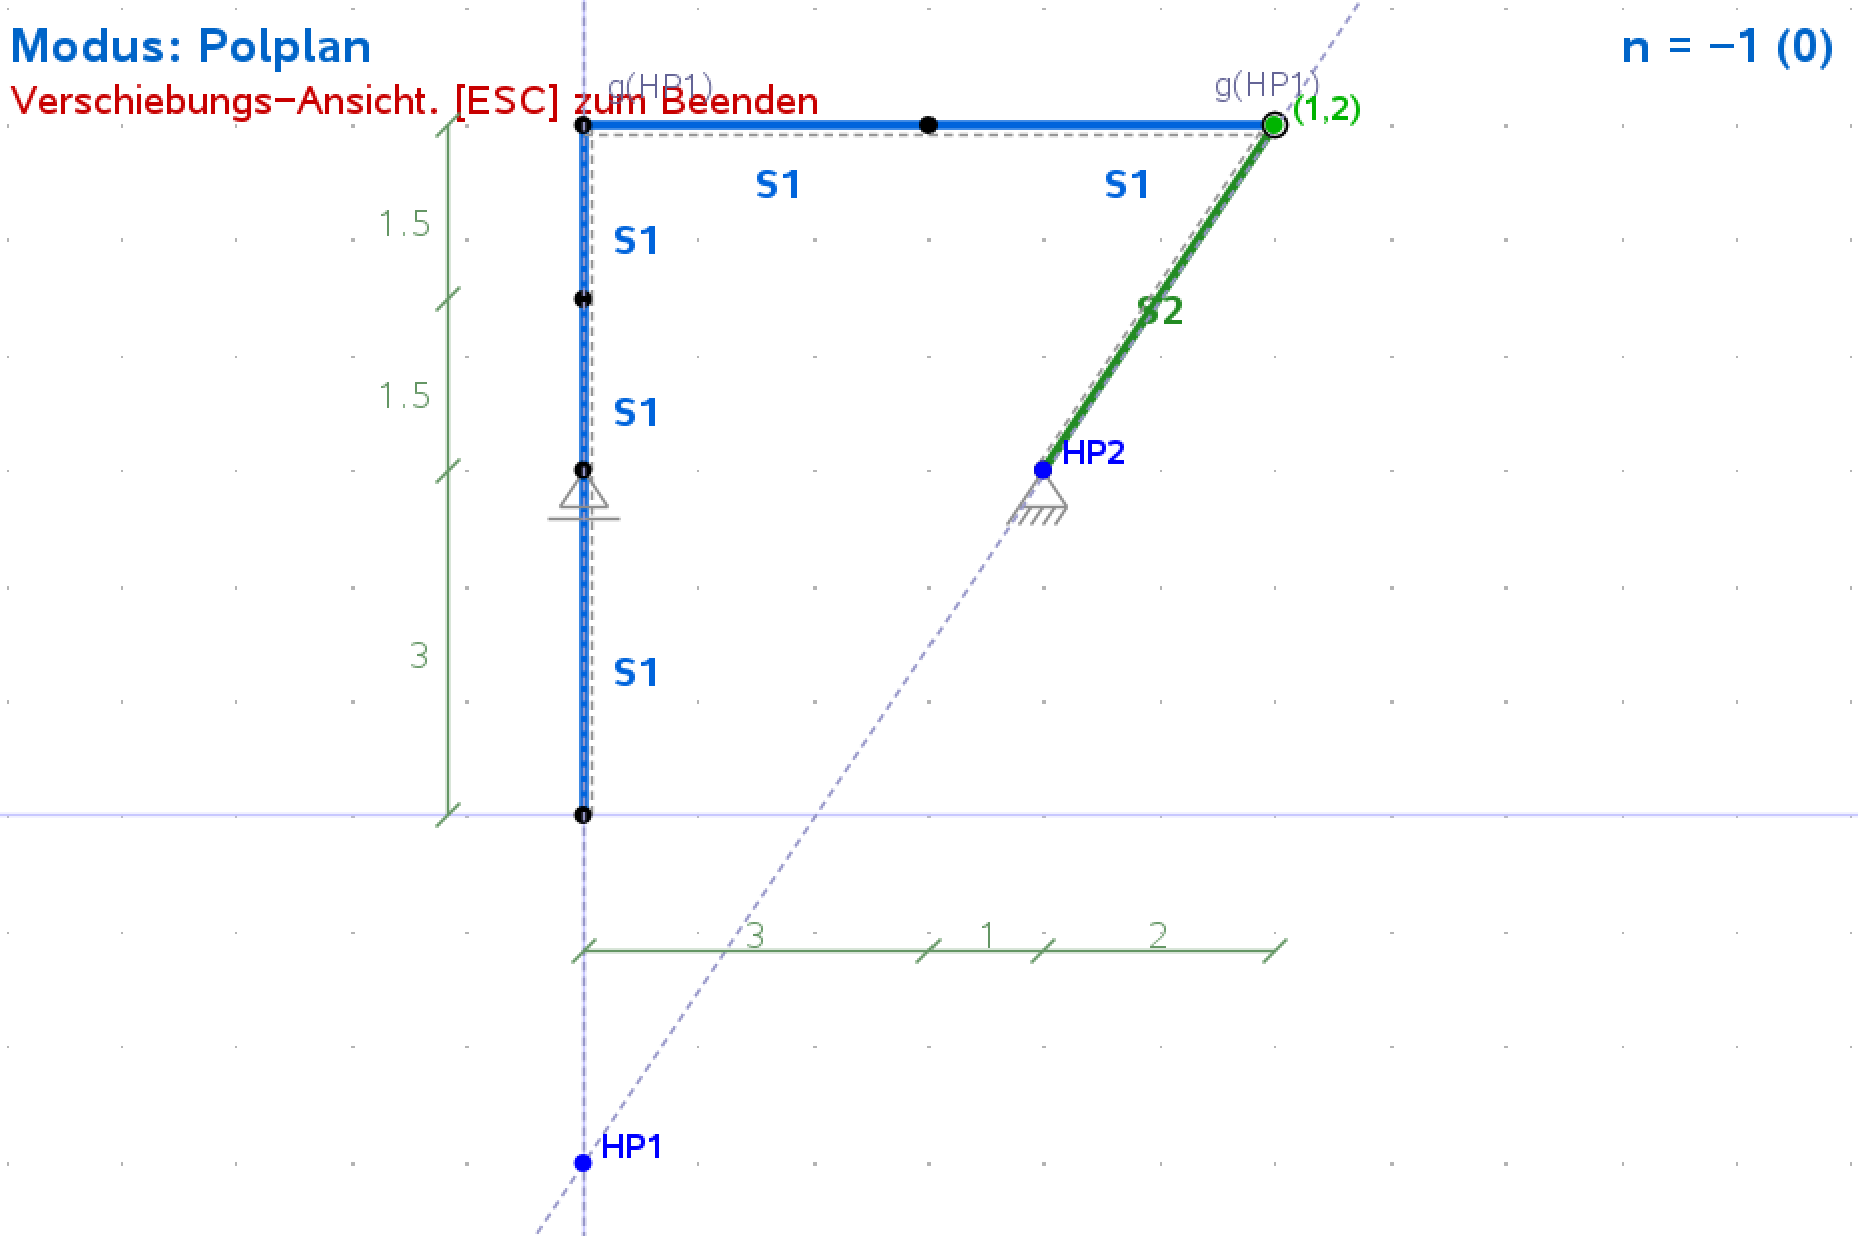
\includegraphics[width=\linewidth]{./fig/TM1/WiSe2122nr3_3.png}
        \caption{Polplan für $A_H$}
    \end{subfigure}
    \caption{WiSe~21/22, Nr.~3: $A_H$}
    \label{fig:TM1WiSe2122Nr3_2}
\end{figure}

\begin{figure}[htbp]
    \centering
    \begin{subfigure}[t]{0.48\textwidth}
        \centering
        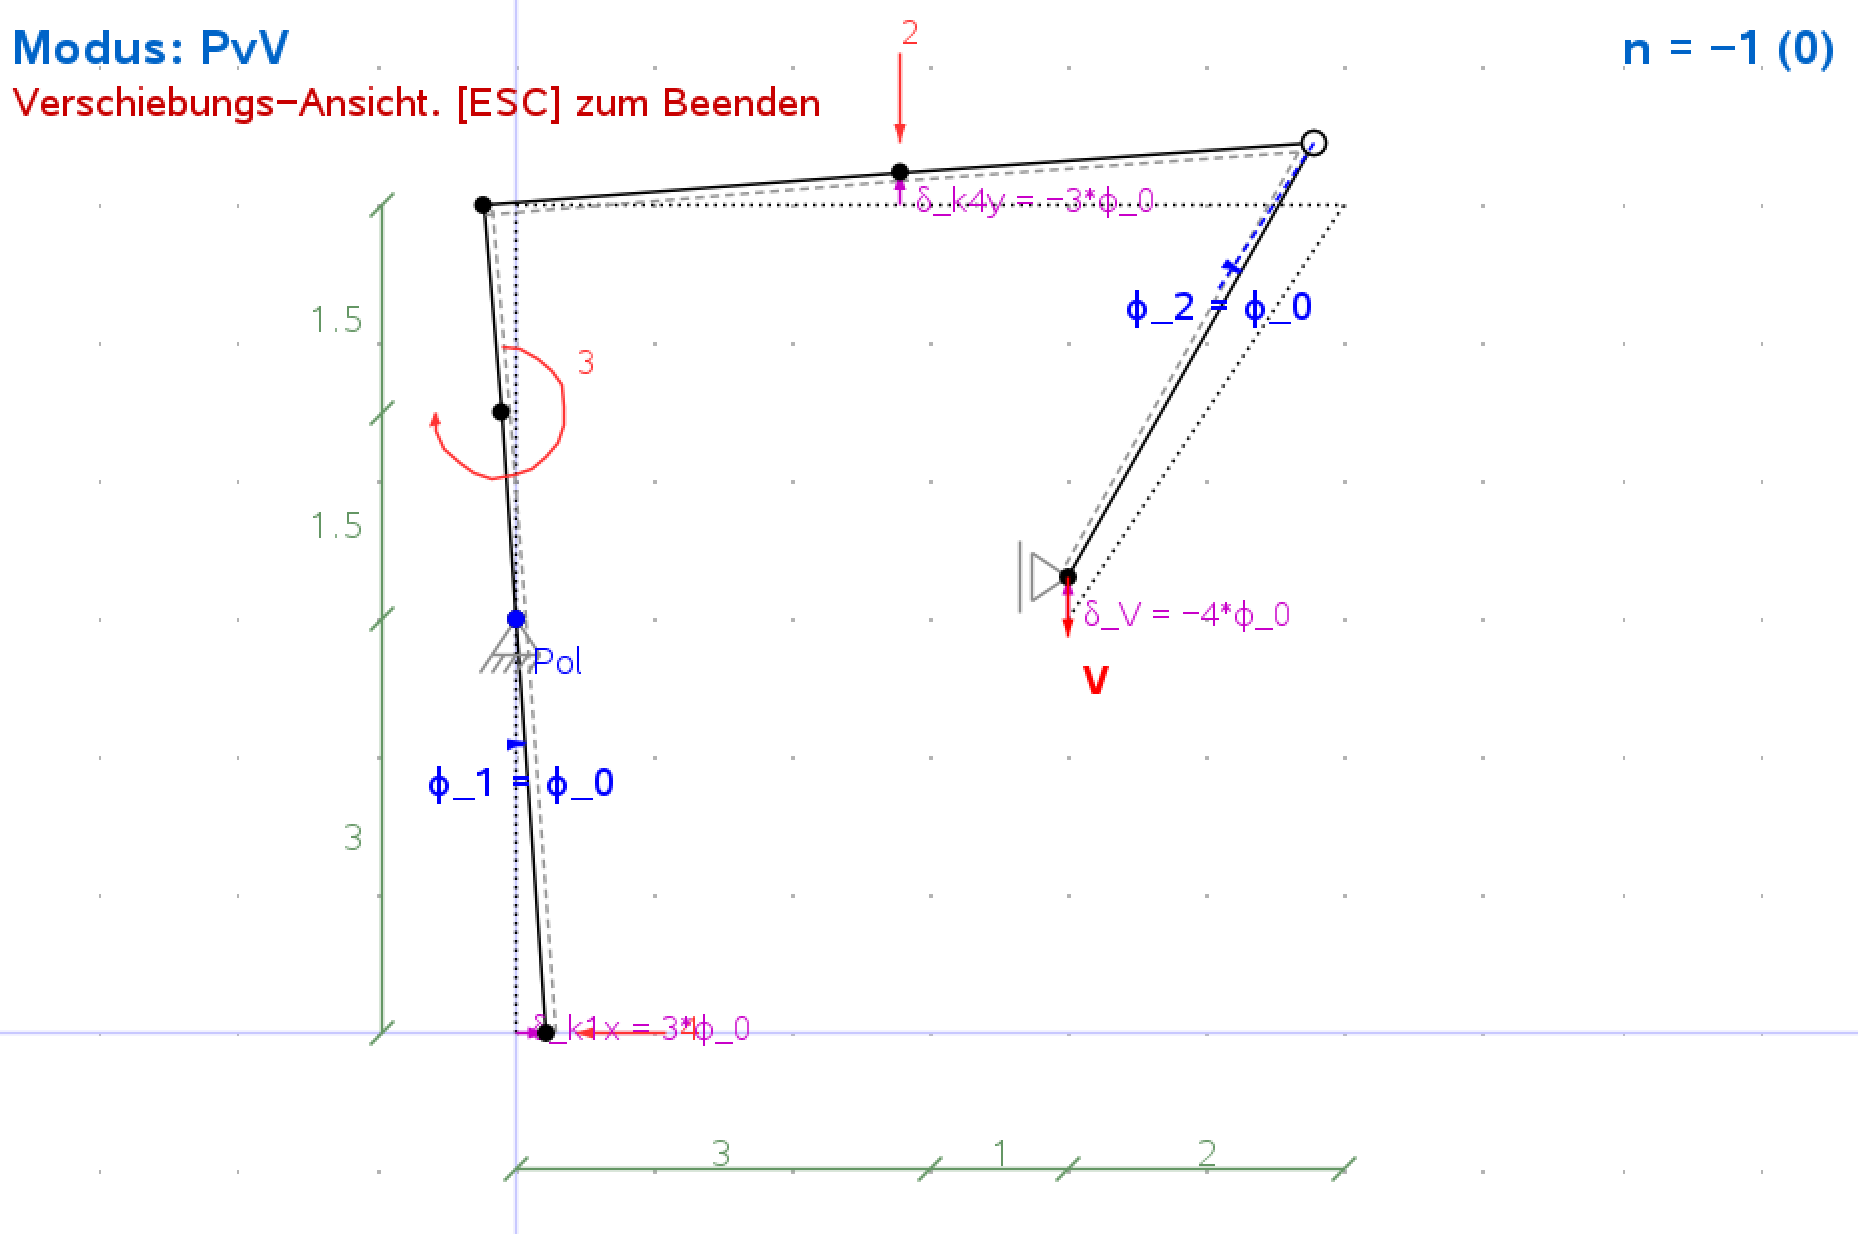
\includegraphics[width=\linewidth]{./fig/TM1/WiSe2122nr3_4.png}
        \caption{Verschiebungsfigur für $B_V$}
    \end{subfigure}
    \hfill
    \begin{subfigure}[t]{0.48\textwidth}
        \centering
        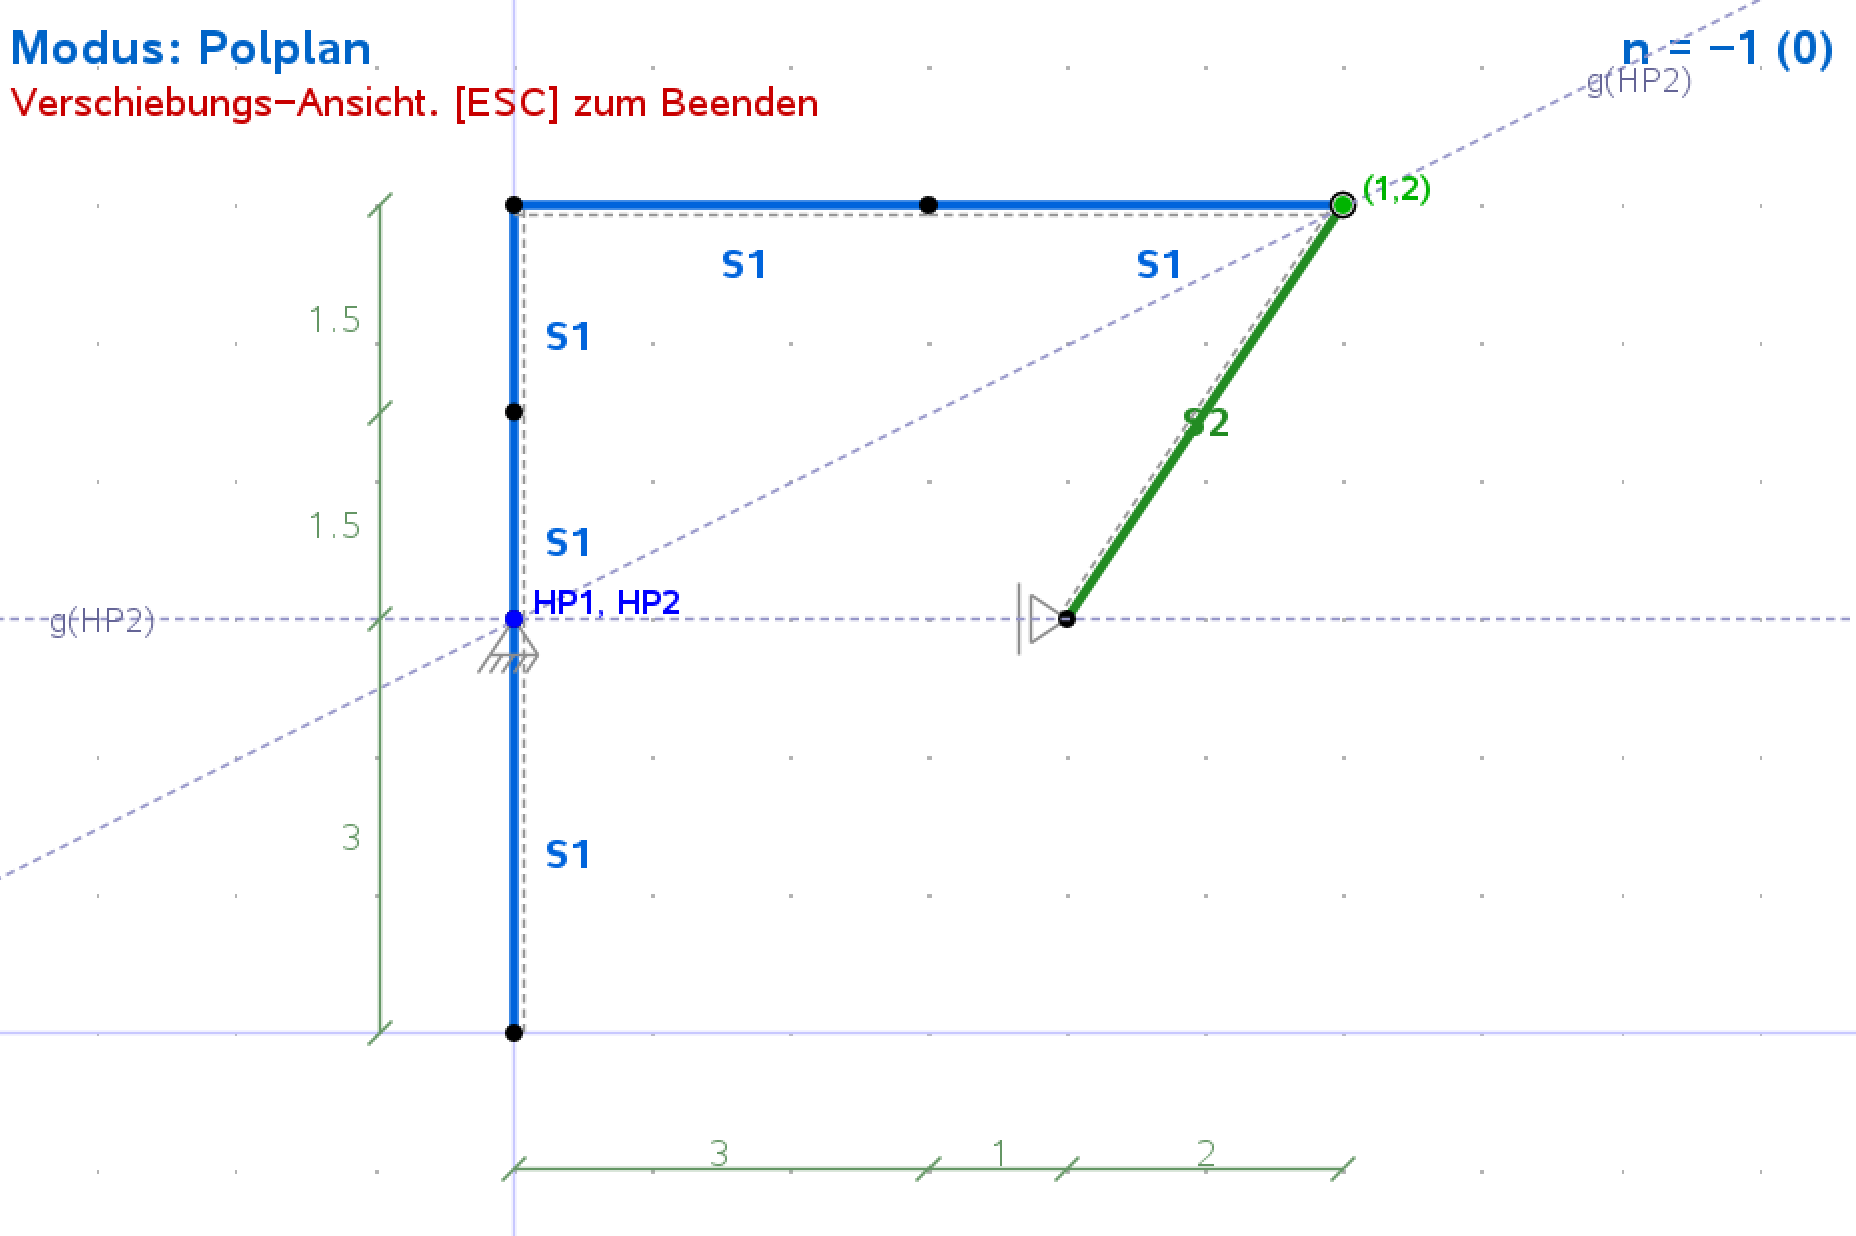
\includegraphics[width=\linewidth]{./fig/TM1/WiSe2122nr3_5.png}
        \caption{Polplan für $B_V$}
    \end{subfigure}
    \caption{WiSe~21/22, Nr.~3: $B_V$}
    \label{fig:TM1WiSe2122Nr3_3}
\end{figure}

Die Zeilen der Matrizen \code{pvv\_kin} und \code{pvv\_pol} (Abb.~\ref{fig:TM1WiSe2122Nr3_4})
sind als Gleichungskette zu lesen. Hier gilt also z.B. $\delta_{k1x}= -3\cdot\varphi_1=-\varphi_0$, oder 
$\delta x_{p12}= -9\cdot\varphi_1=-3\varphi_2$. Mit diesen Gleichungen lässt sich aus \code{w\_eq1} \code{w\_eq2} bauen.
Diese gleichung lässt sich dann entweder von hand oder mit dem Taschenrechner nach der gesuchten Größe auflösen.

\begin{figure}[htbp]
    \centering
    \begin{subfigure}[t]{0.48\textwidth}
        \centering
        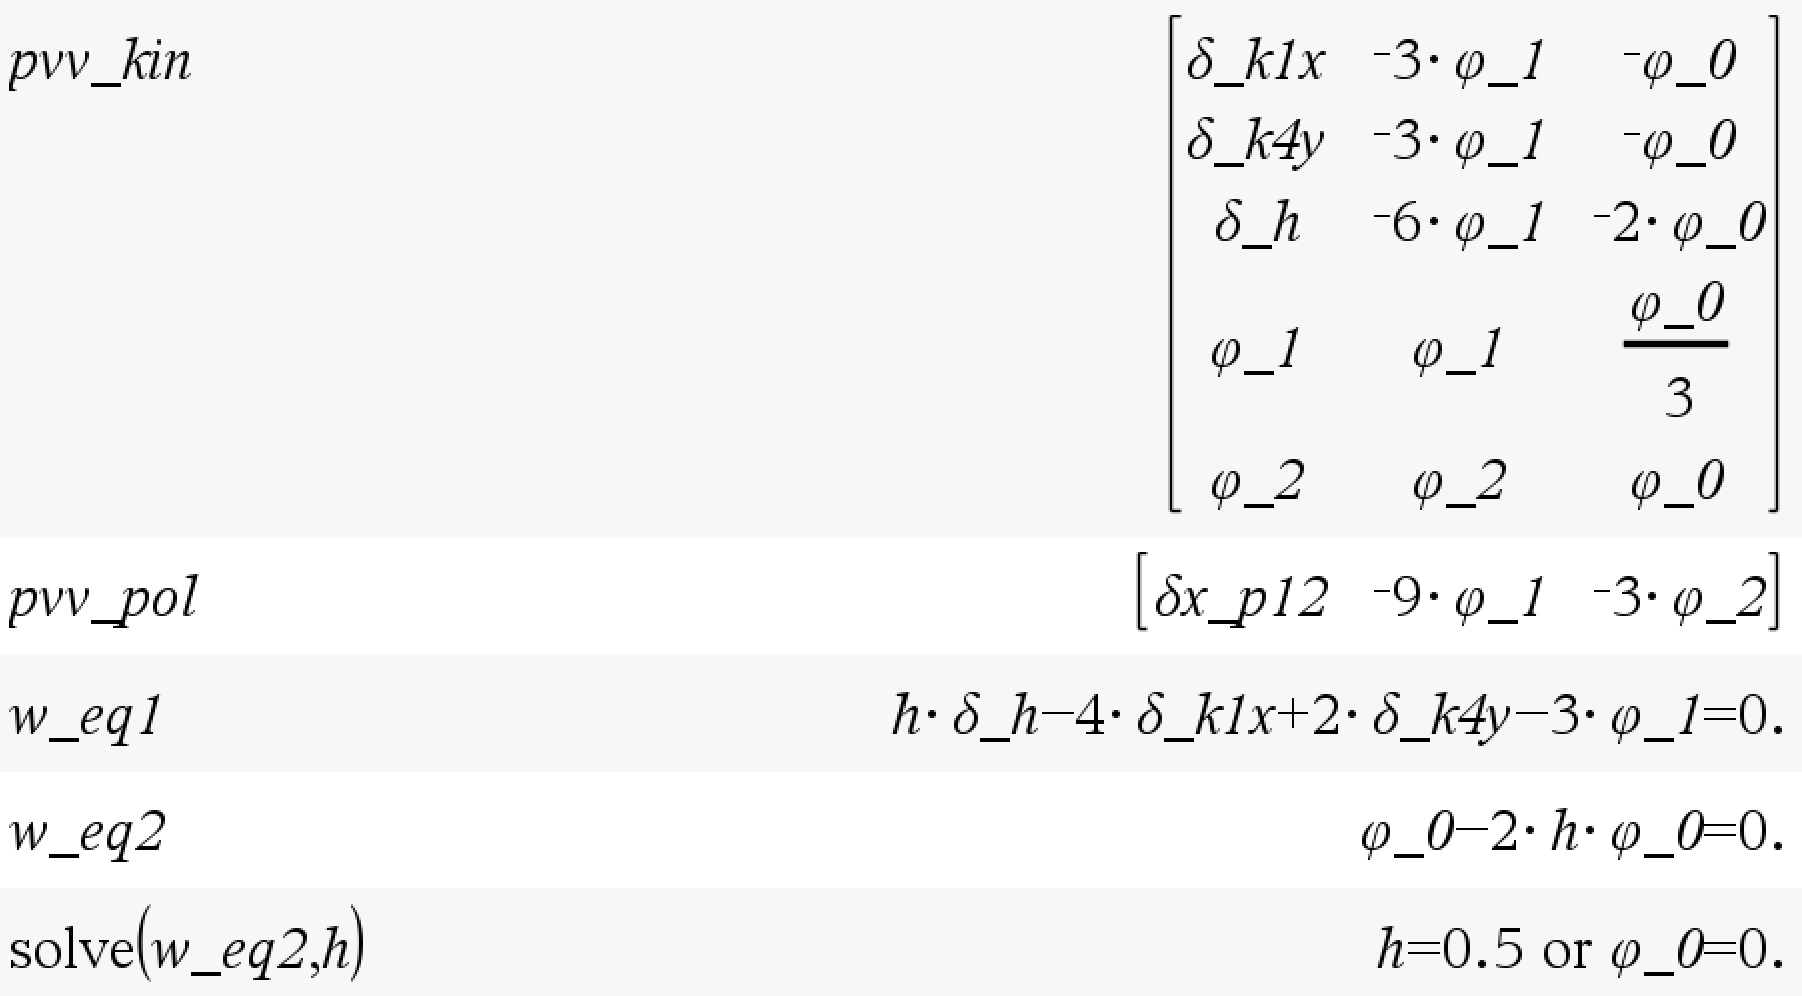
\includegraphics[width=\linewidth]{./fig/TM1/WiSe2122nr3_6.png}
        \caption{Rechnung für $A_H$}
    \end{subfigure}
    \hfill
    \begin{subfigure}[t]{0.48\textwidth}
        \centering
        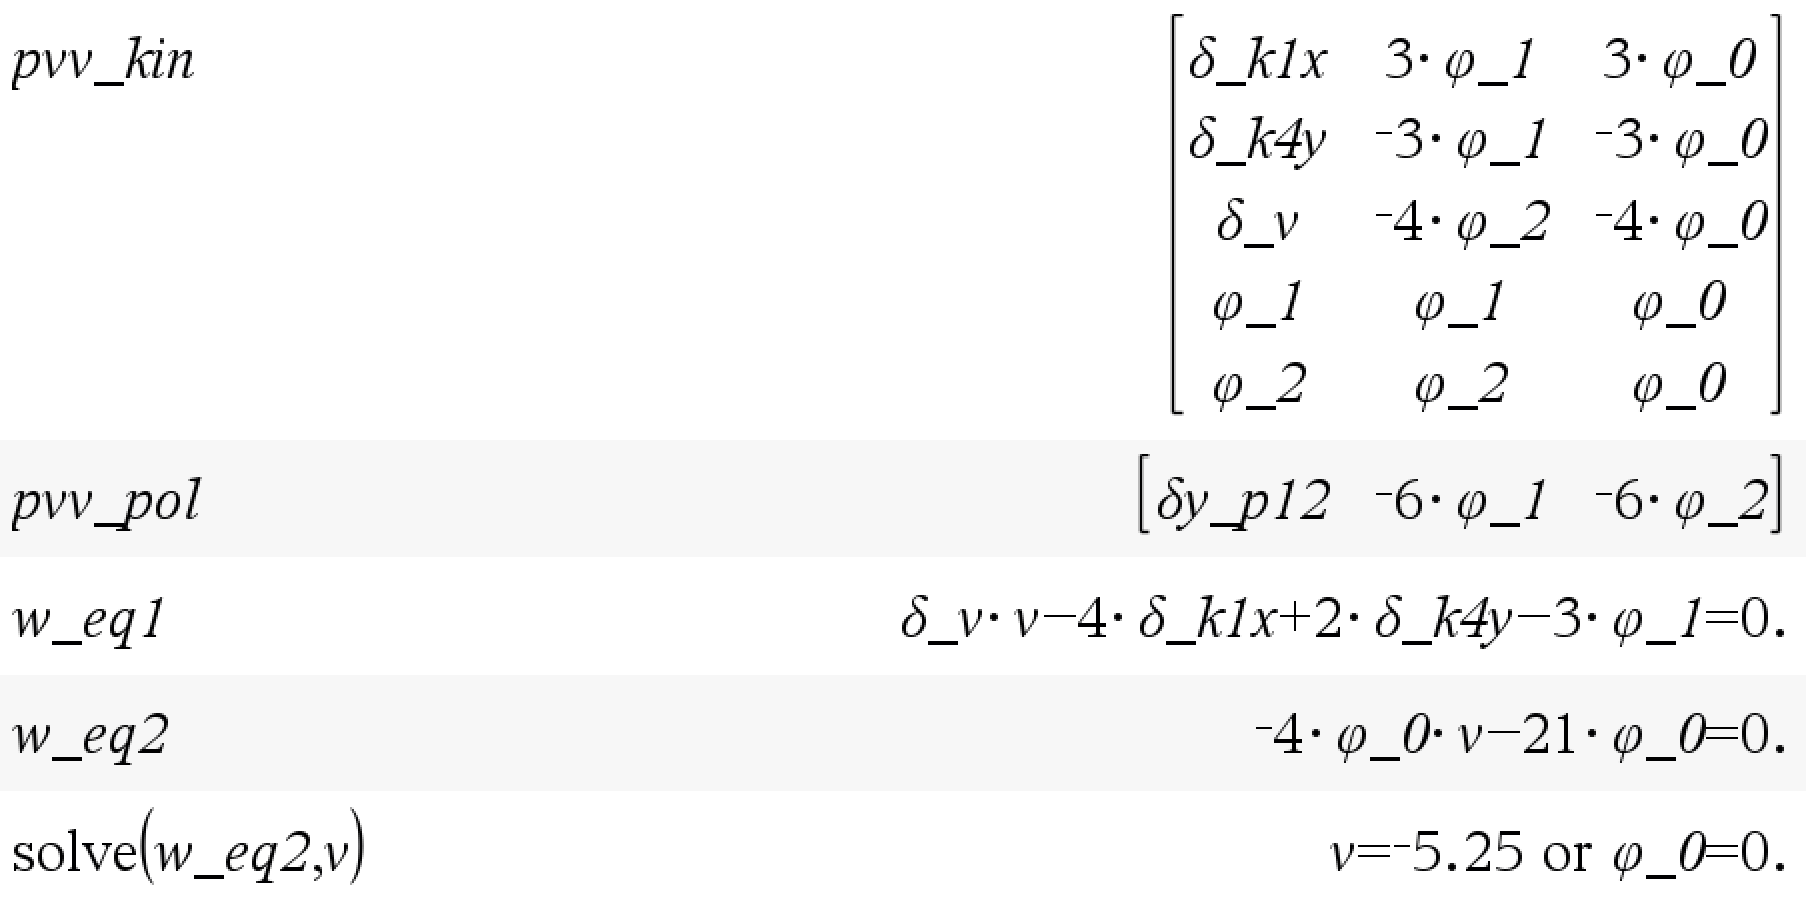
\includegraphics[width=\linewidth]{./fig/TM1/WiSe2122nr3_7.png}
        \caption{Rechnung für $B_V$}
    \end{subfigure}
    \caption{WiSe~21/22, Nr.~3: Ergebnis}
    \label{fig:TM1WiSe2122Nr3_4}
\end{figure}

\subsection{Schnittkräfte Bögen (Nr.~5)}

Mit dem Programm lassen sich die Funktionen für Schnittkraftverläufe von normalen Stäben als auch von Bögen 
ausgeben. Bei bögen ist die Laufvraibale nur nicht mehr die Länge entlang des Stabes sondern der Winkel.
also für diese Aufgabe zweilmal $\varphi \in [0,\frac{\pi}{4}]$ bzw. $\varphi \in [0,90\text{°}]$. Hier ist die Winkel-Einstellung
des Taschenrechenrs wichtig.\\
Hier gilt aber auch wieder, dass das Programm das nicht wirklich so ausrechnet wie man das von Hand machen würde, sondern
es sucht eine schöne Darstellung der Anfangswerte und kombiniert diese dann zur Funktion.

\begin{figure}[htbp]
    \centering
    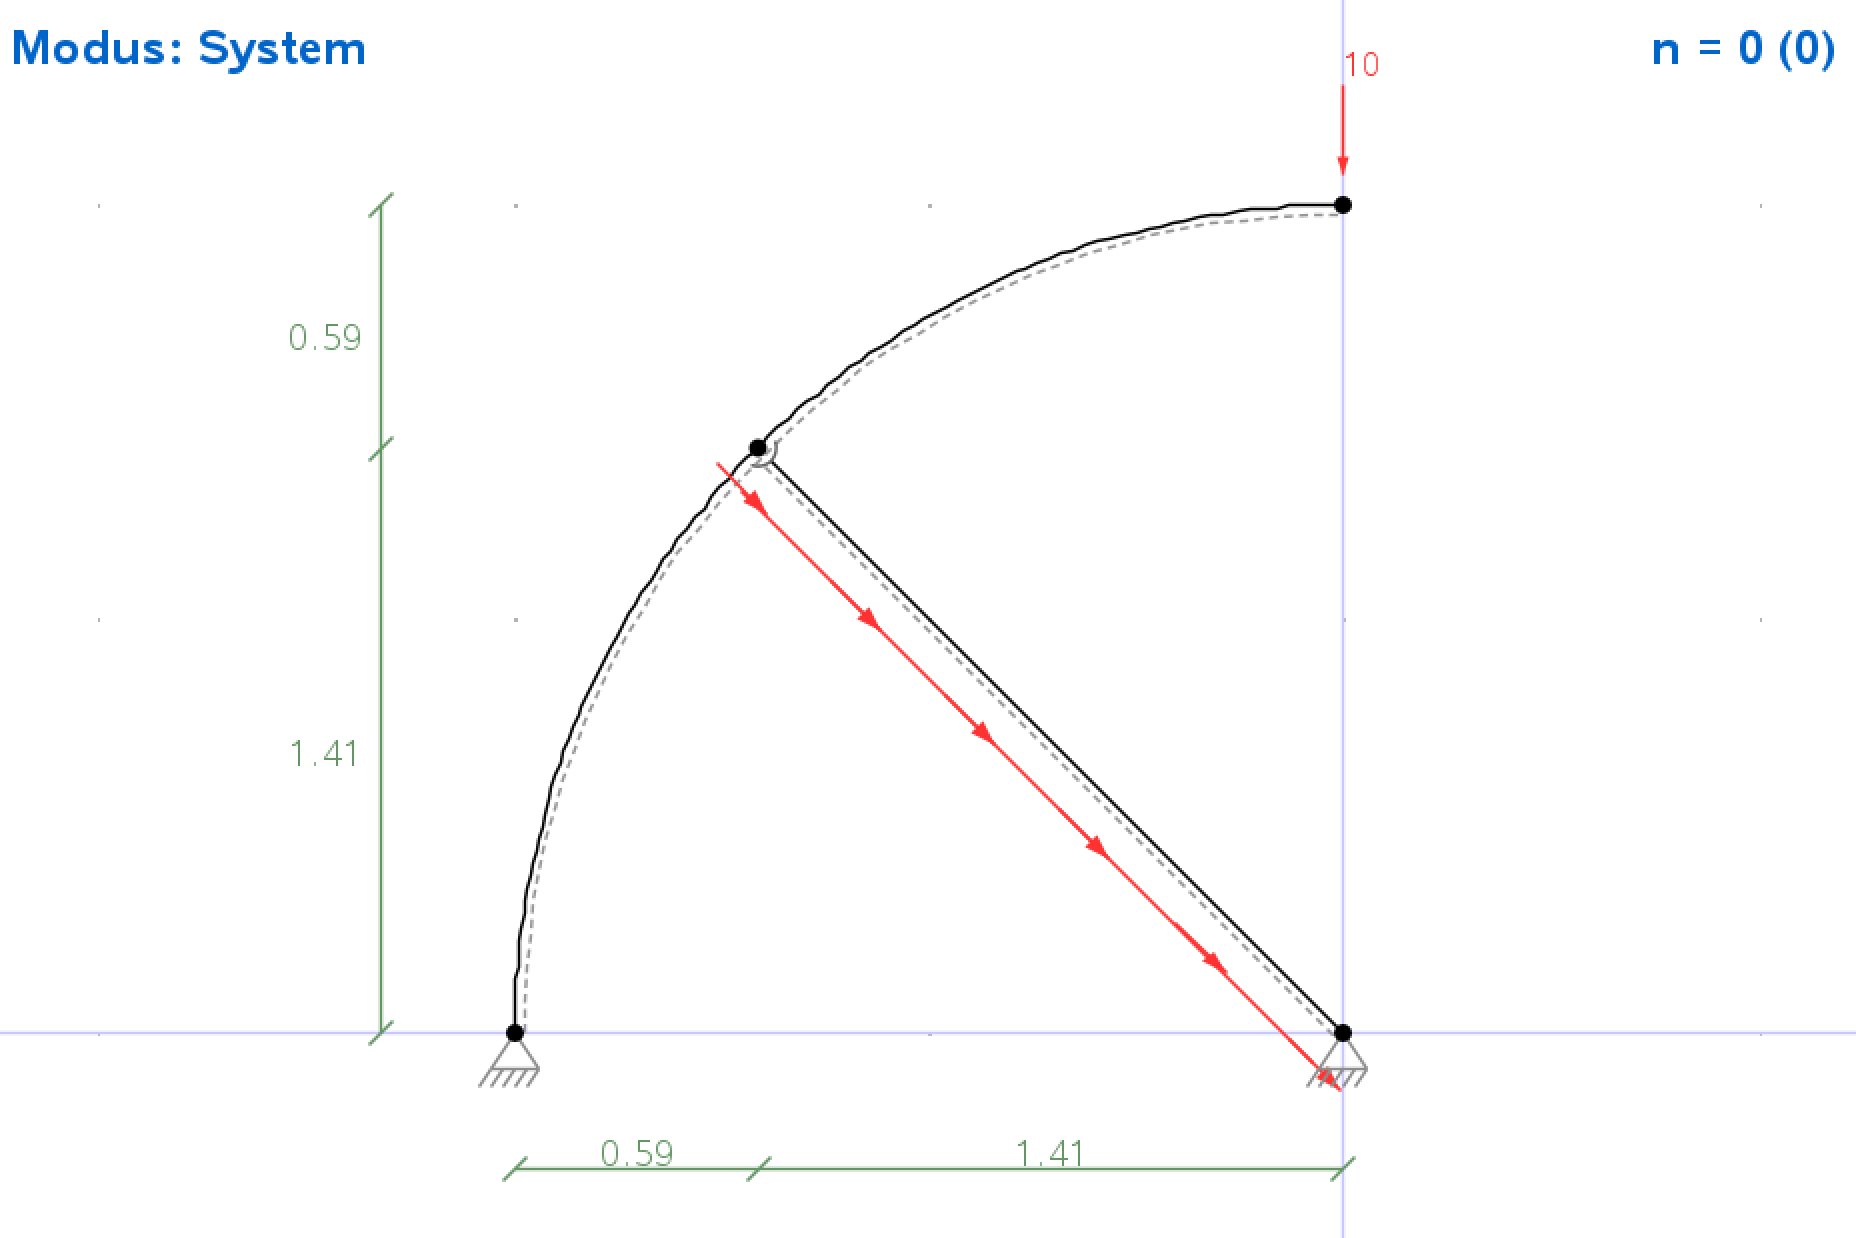
\includegraphics[width=0.5\linewidth]{./fig/TM1/WiSe2122nr5_1.png}
    \caption{TM1 WiSe~21/22, Nr.~5 im Programm}
    \label{fig:TM1WiSe2122Nr5_1}
\end{figure}


\subsection{Fachwerk (Nr.6)}

Vom Prinzip werden Fachwerke genau gleich eingegeben wie normale Systeme, nur das hier die orientierung der gestrichelten Faser
keine Rolle spielt. Es ist jedoch sinnvoll den Fachwerk Modus anzumachen, dann wird die statische Bestimmtheit beim hovern über $n=$ 
auch die Formel für Fachwerke verwendet und alle Knoten werden zu vollgelenken gemacht, auch wenn der Modus erst nach dem 
zeichnen des Systems angemacht wird.  


\begin{figure}[htbp]
    \centering
    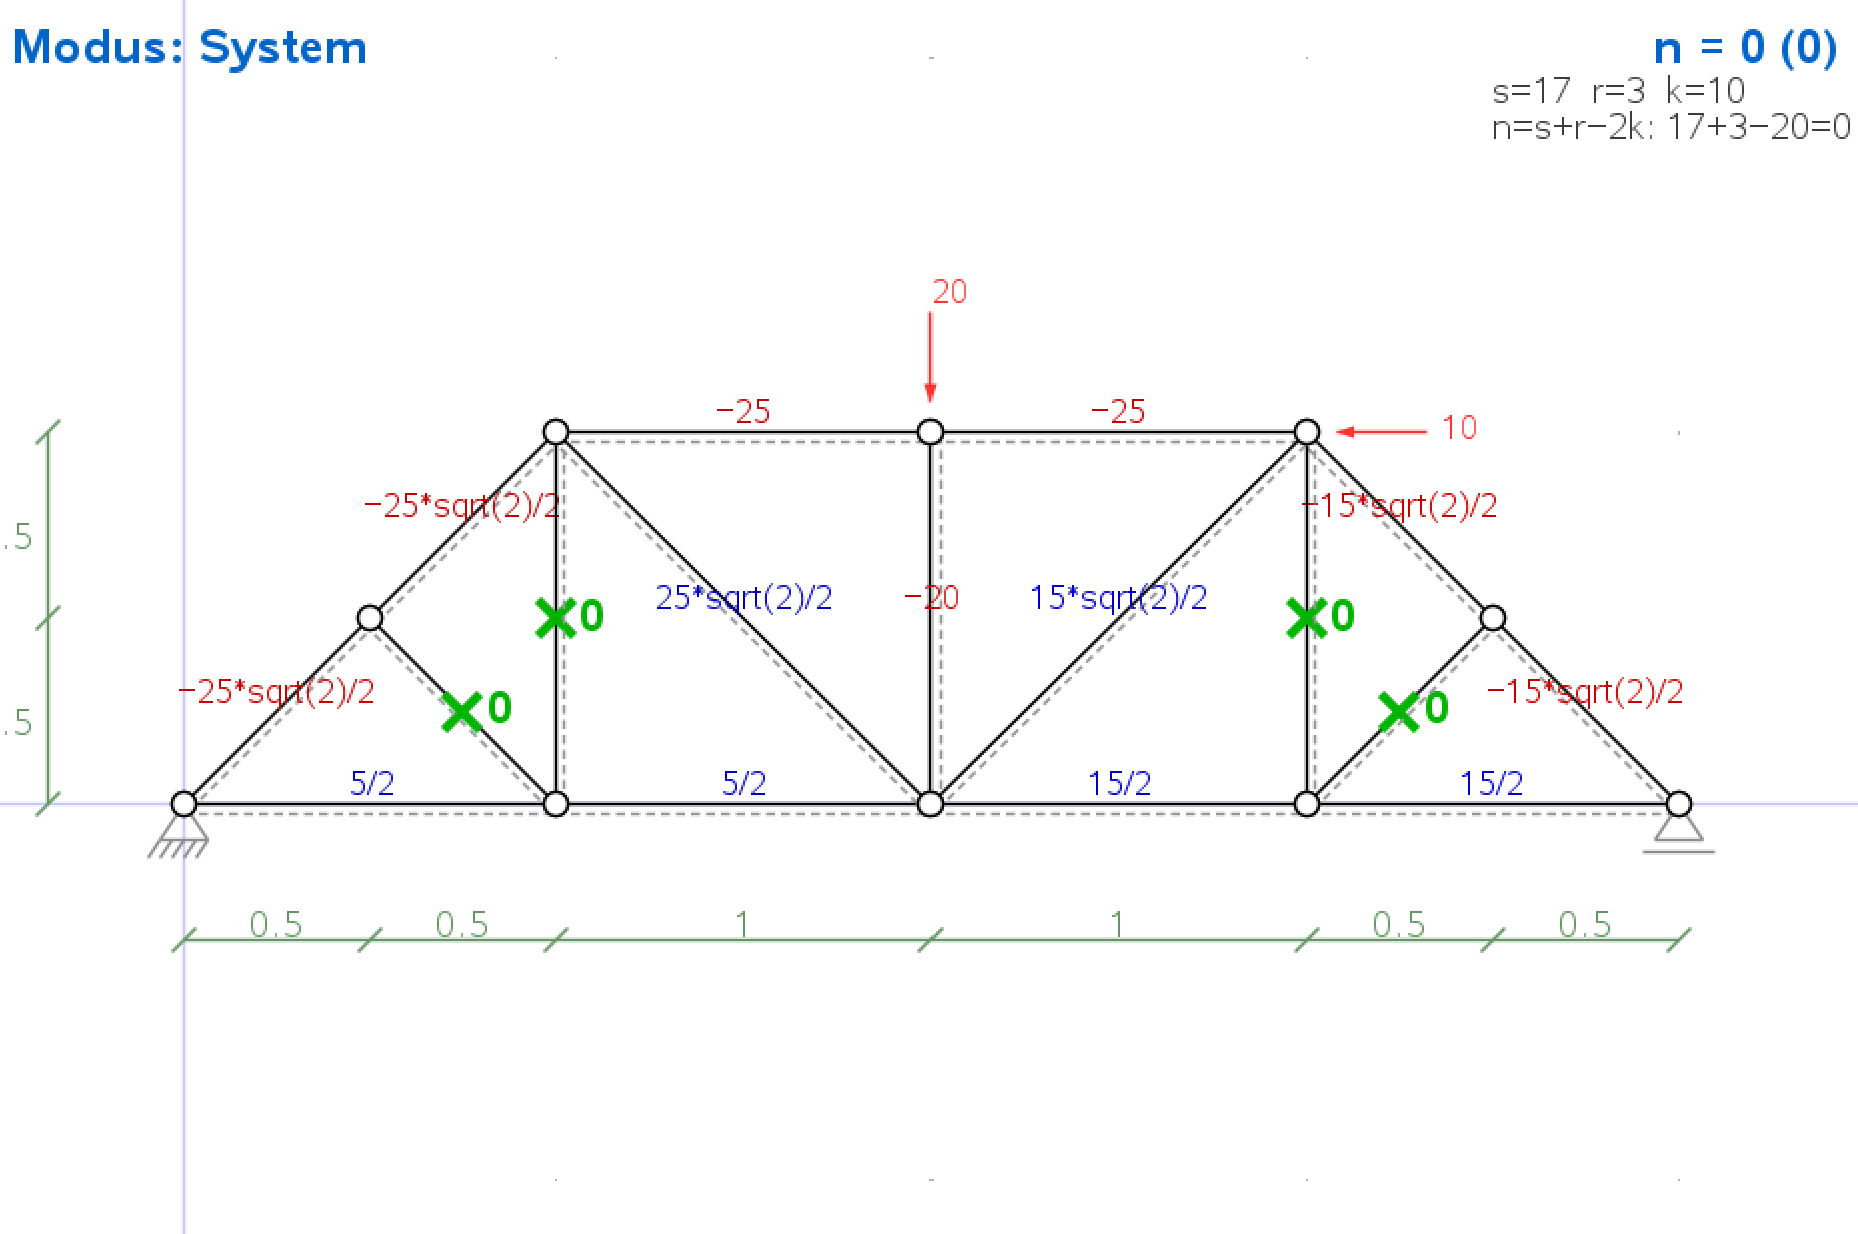
\includegraphics[width=0.5\linewidth]{./fig/TM1/WiSe2122nr6_1.png}
    \caption{TM1 WiSe~21/22, Nr.~6 im Programm}
    \label{fig:TM1WiSe2122Nr6_1}
\end{figure}

Die Stabe in Abb.~\ref{fig:TM1WiSe2122Nr6_1} die ein grünes Kreuz haben sind die ohne Rechnung erkennbaren Nullstäbe
Falls nach der Berechnung stäbkkräfte mit einer grünen Null beschriftet werdsen, aber dort kein Kreuz ist, ist das zwar ein 
Nullstab der aber nicht direkt aus den Regeln erkennbar ist. Für Afgaben bei denen nach Nullstäben gefragt wird, also nur 
die durchgekreuzten Stäbe angeben

\begin{figure}[htbp]
    \centering
    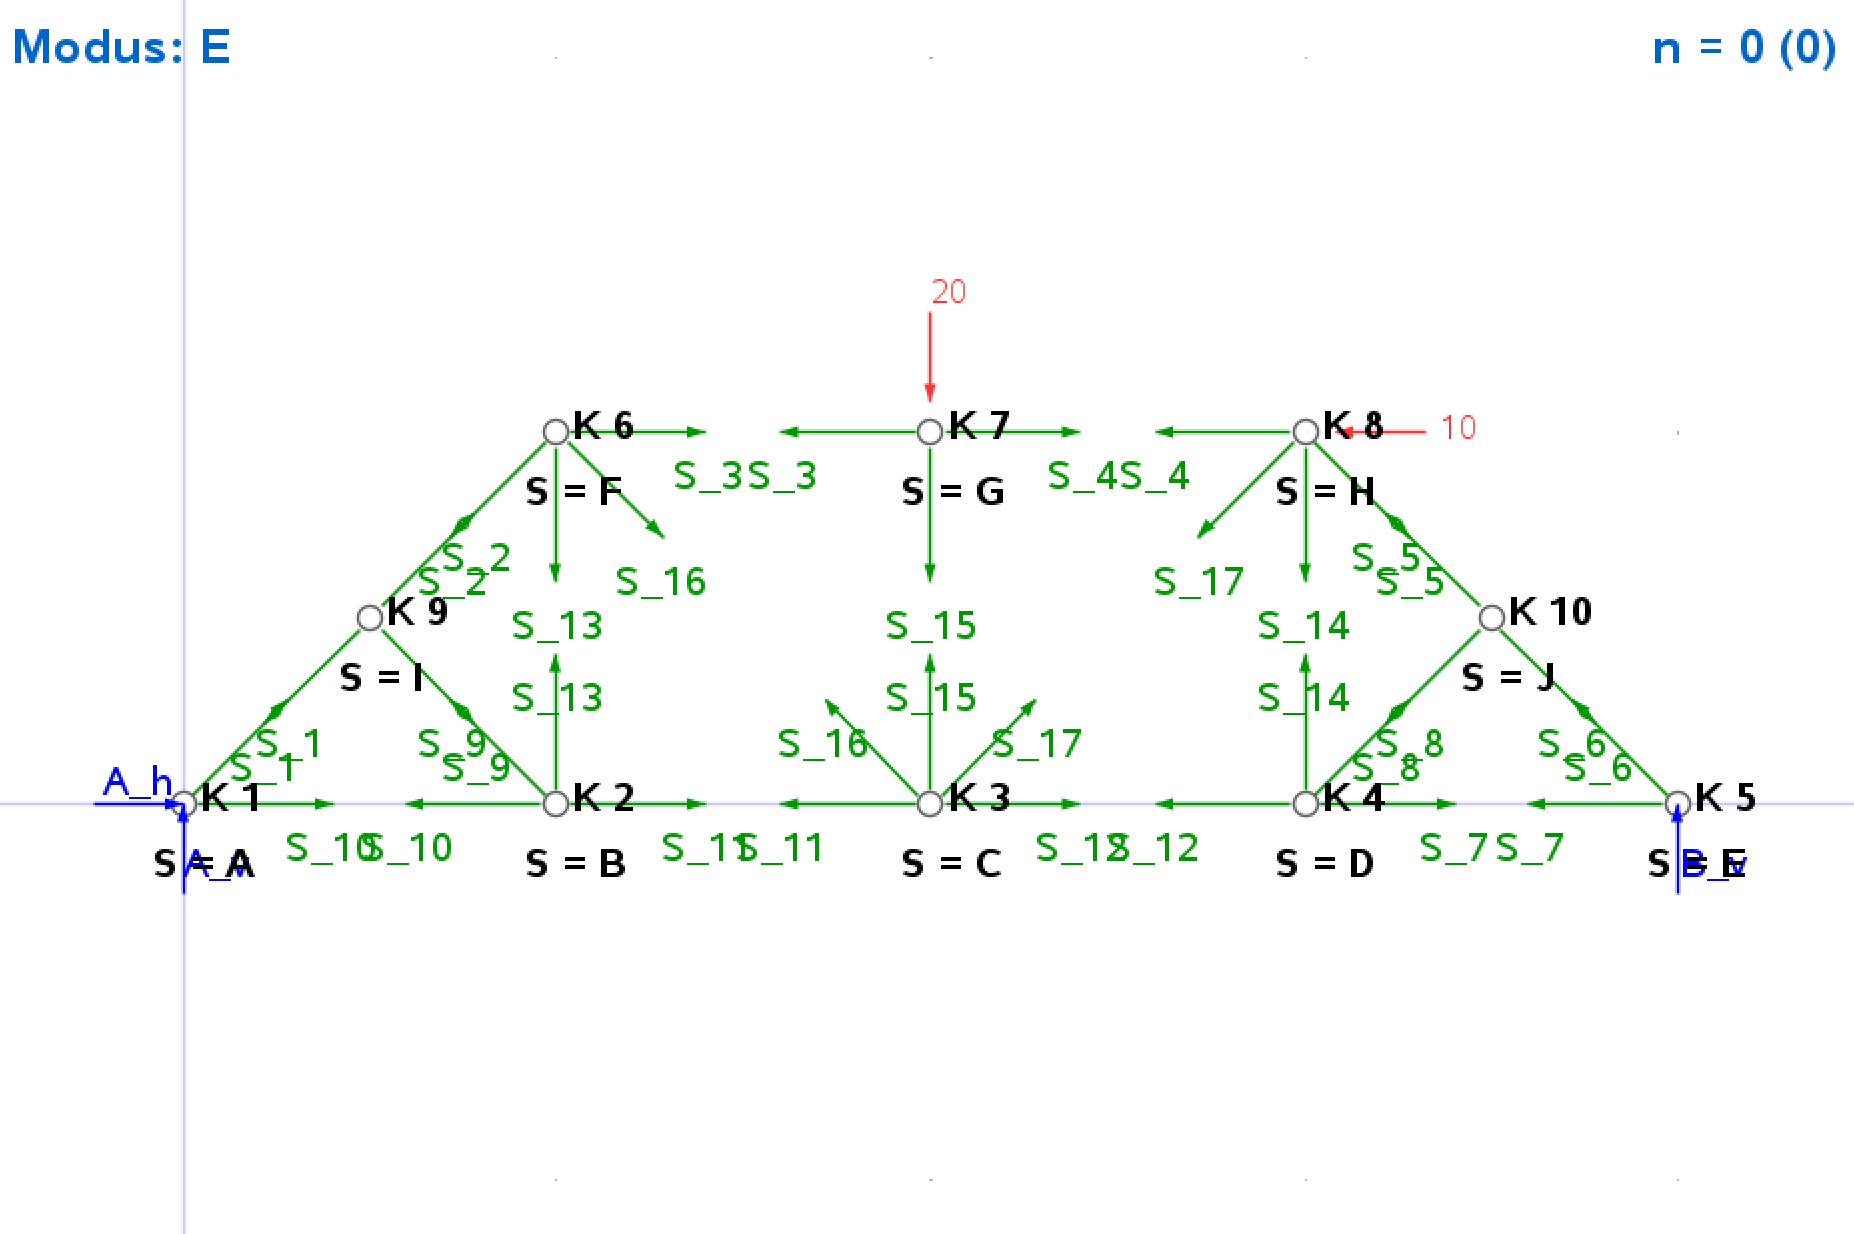
\includegraphics[width=0.5\linewidth]{./fig/TM1/WiSe2122nr6_2.png}
    \caption{TM1 WiSe~21/22 Freischnitt}
    \label{fig:TM1WiSe2122Nr6_2}
\end{figure}

Für die Verwendung der beiden Seiten des E-Modus muss darauf geachtet werden, dass entweder die Stäbe in der
gleichen Reihenfolge wie in der Aufgabe gezeichnet werden oder die Bennenung hinterher angepasst wird. Macht ihr das nicht
ist z.B. Stab 13 aus eurer Rechnung nicht Stab 13 aus der Aufgabe\\
Gleiches gilt natürlich auch für die Verwendung des LGS-Exports. Hier wird (Falls der Fachwerk Modus an ist) 
das Knotenschnittverfahren verwendet. Die Benennung im LGS ist die gleiche wie auf der zweiten Seite des E-Modus.





\section{TM2}

\subsection{Biegelinie (TM2 WiSe~21/22, Nr.~7)} \label{ex:Biegelinienaufgabe}

In dieser Aufgabe ist ein \emph{interessantes} KOS vorgegeben: Soll es ein Rechtssystem sein,
zeigt die $y$-Achse hier in die Zeichenebene hinein und nicht, wie sonst üblich, aus ihr heraus.

Rechnet ihr von Hand über die DGL $EI\,w'''' = q$ mit allen Rand- und Übergangsbedingungen (so
geht man bei statisch unbestimmten Systemen meist vor, und so rechnet auch \code{wneu}), gibt es
hier nichts weiter zu beachten. Bei einem statisch bestimmten System lohnt es sich dagegen, zuerst
die Momentenlinie zu berechnen und dann $EI\,w'' = -M$ zu integrieren. Dafür braucht ihr die
gestrichelte Faser. Die Regel aus Abschnitt~\ref{sec:Eingabe_Stäbe}, dass sie immer auf der Seite
liegt, in die die $z$- bzw.\ $w$-Achse zeigt, gilt auch hier. Alternativ könnt ihr euch überlegen,
auf welcher Seite ein positives Schnittmoment $M_y$ (Drehsinn nach der Rechte-Hand-Regel um die
$y$-Achse) Zug erzeugt, dort liegt die gestrichelte Faser. Das finde ich aber umständlicher.

Im Programm müsst ihr solche Systeme etwas anders eingeben, denn dort zeigt die $y$-Achse immer
aus der Zeichenebene heraus. Zeichnet ihr das System genau wie in der Aufgabe und setzt die
gestrichelte Faser nach der Regel oben, läuft die $x$-Koordinate im Programm in die andere Richtung
als in der Aufgabe. Um das zu umgehen, zeichnet ihr Systeme, bei denen die $y$-Achse in die
Zeichenebene hineinzeigt, spiegelverkehrt (Abb.~\ref{fig:Biegelinienaufgabe}). Ich habe die
Aufgabe im symbolischen Modus gerechnet, deshalb stehen in den Ergebnissen $q$ und $l$.

\begin{figure}[htbp]
    \centering
    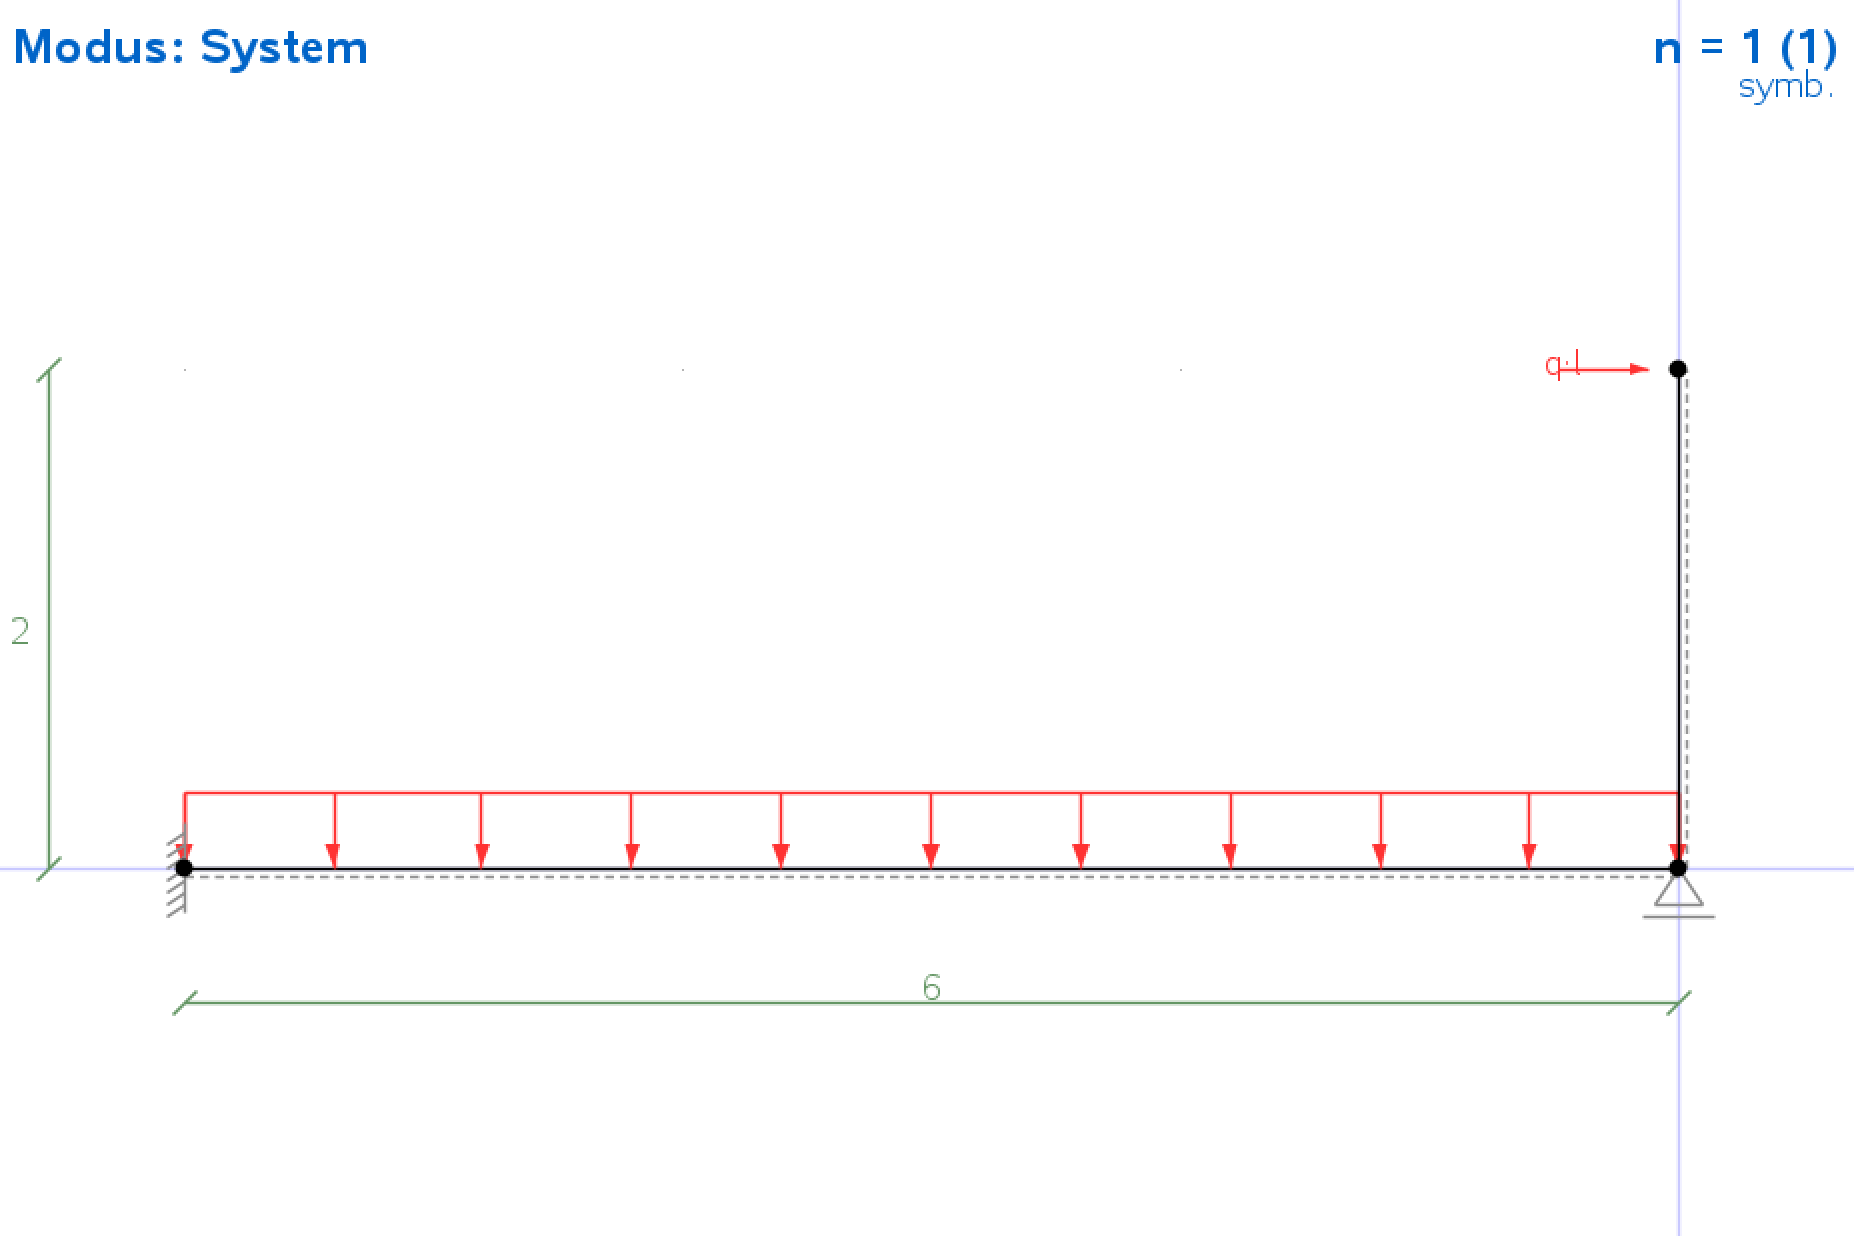
\includegraphics[width=0.5\linewidth]{./fig/TM2/WiSe2122nr7_1.png}
    \caption{TM2 WiSe~21/22, Nr.~7 im Programm, spiegelverkehrt gezeichnet}
    \label{fig:Biegelinienaufgabe}
\end{figure}

Das liefert die Ergebnisse in Abb.~\ref{fig:BiegelinienaufgabeBiegelinie}. Hier geben beide
Methoden dasselbe Ergebnis. Das sollte natürlich so sein, ist aber nicht immer so: Manchmal weicht
die WGV/FEM-Lösung \code{v\_EI\_stab1(x)} (im Rechner klein geschrieben) minimal von der exakten
Lösung \code{wneu1(x)} ab. Weil das Programm die Brüche aus den Zahlen der FEM-Lösung
\emph{errät} (Abschnitt~\ref{sec:mathe-symbolisch}), kann daraus eine ganz anders aussehende
Biegelinie werden. Die Methode über die WGV/FEM-Lösung gibt es trotzdem, vor allem weil ich sie
zuerst programmiert habe (daher wohl auch der Name \code{wneu} der anderen Funktion), und weil sie
bei sehr großen Systemen deutlich schneller sein kann.

\begin{figure}[htbp]
    \centering
    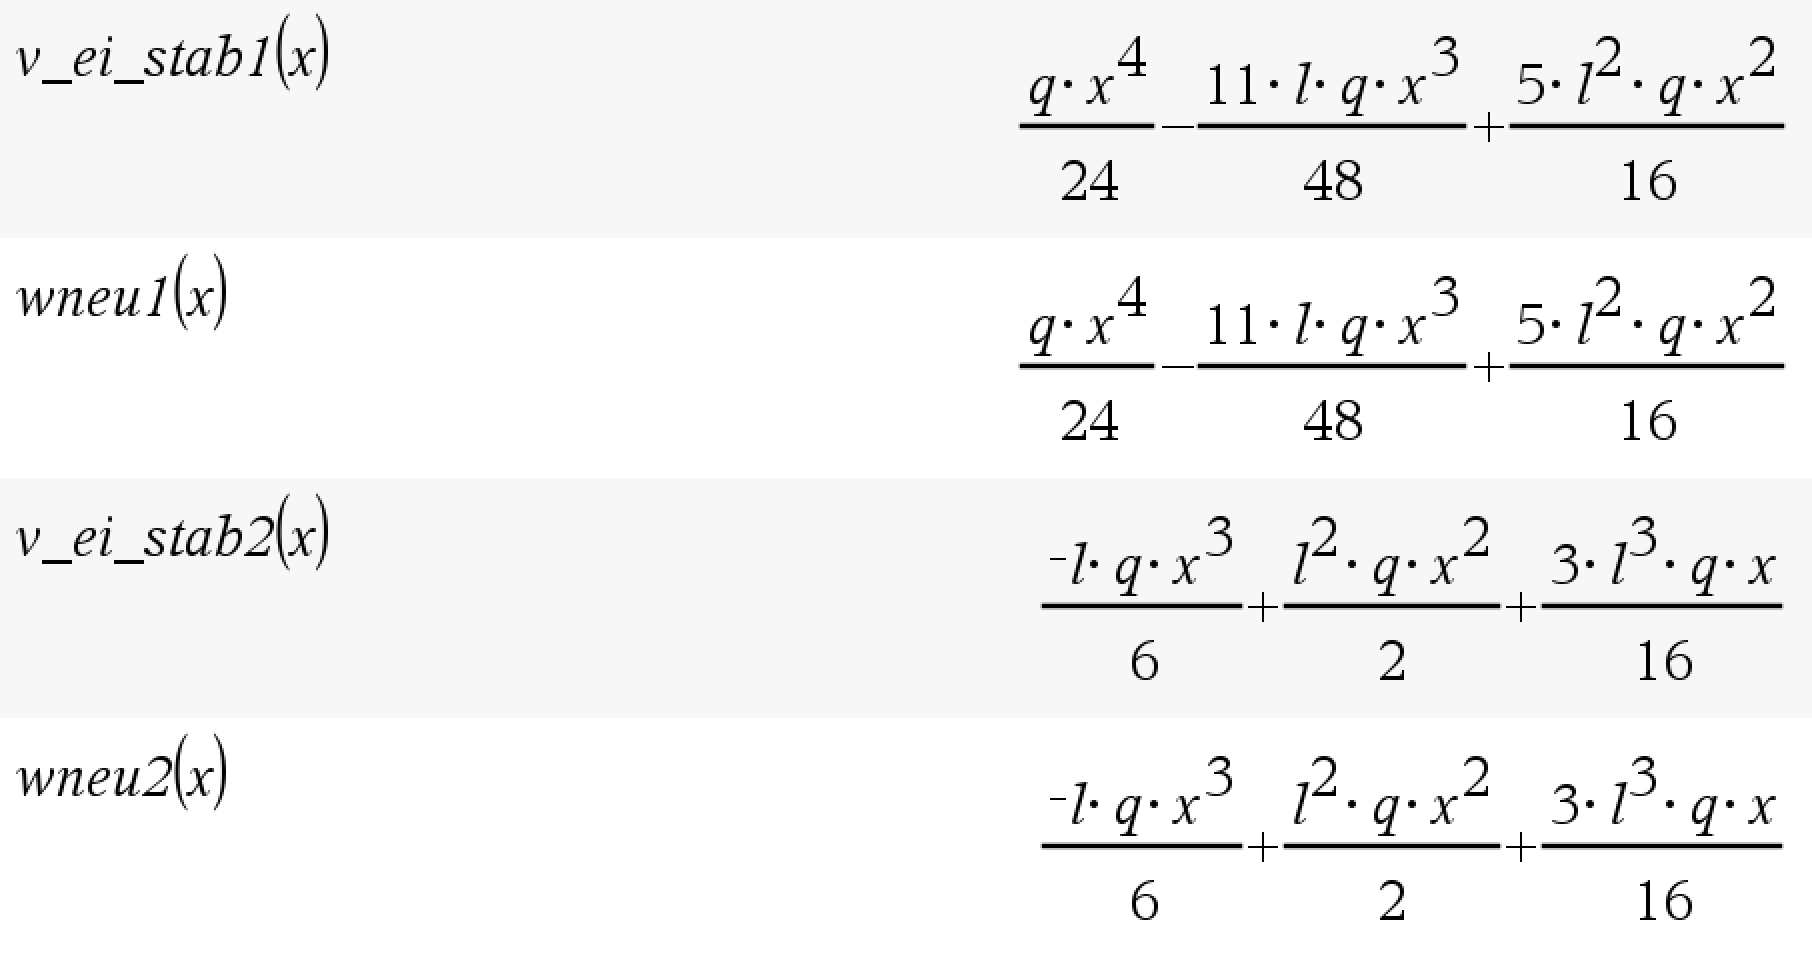
\includegraphics[width=0.5\linewidth]{./fig/TM2/WiSe2122nr7_2.png}
    \caption{TM2 WiSe~21/22, Nr.~7: \code{v\_EI\_stab} und \code{wneu} im Vergleich}
    \label{fig:BiegelinienaufgabeBiegelinie}
\end{figure}

Weil die Stäbe dehnsteif sind, kann das Programm hier sogar die Randbedingungen für Biegelinie und
Längslinie getrennt angeben (Abb.~\ref{fig:BiegelinienaufgabeRandbed}): Die Bedingungen im oberen
Block reichen für die Biegelinie allein, die im unteren kommen nur für die Längslinie dazu. Das geht
nicht immer. Sind die Stäbe dehnbar, hängt die Biegelinie über die Rahmenecken auch von den
Längsverformungen ab, und das Programm gibt alle Bedingungen zusammen aus
(Abschnitt~\ref{sec:randlgs}).

\begin{figure}[htbp]
    \centering
    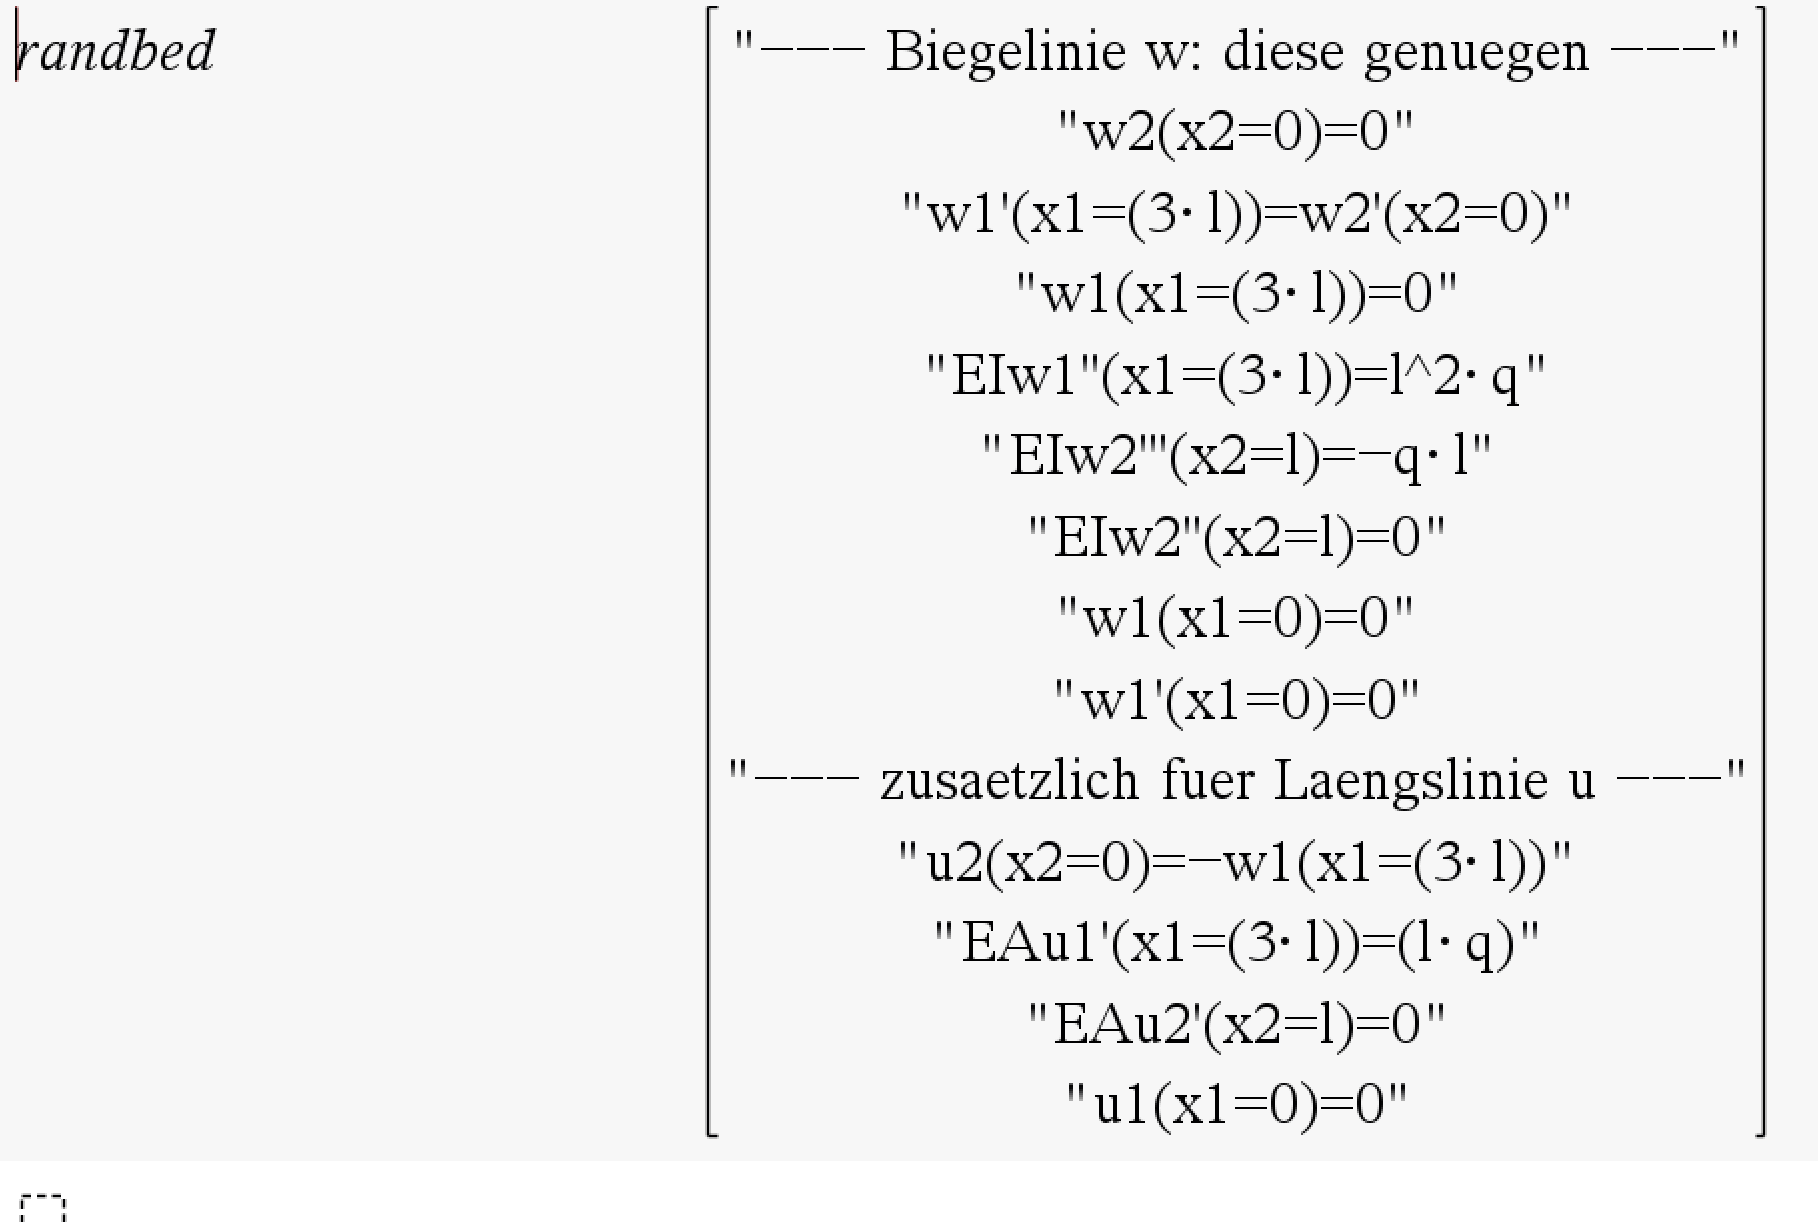
\includegraphics[width=0.5\linewidth]{./fig/TM2/WiSe2122nr7_3.png}
    \caption{Randbedingungen \code{randbed} für TM2 WiSe~21/22, Nr.~7}
    \label{fig:BiegelinienaufgabeRandbed}
\end{figure}



\subsection{Verschiebungsaufgaben (TM2 WiSe~20/21 Nr.~4)} \label{ex:Temperaturaufgabe}

Aufgaben wie diese lassen sich mit der richtigen Eingabe auch direkt im Programm lösen. Wie diese Aufagbe im
Programm aussieht ist in Abb.~\ref{fig:verschiebungSystem} dargestellt. Hierbei muss natürlich auf die Einheiten geachtet werden.
In der Aufgabe sind die relevanten Dehnsteifigkeiten nicht direkt gegeben, genauso wie manche Angaben nicht in der
für das Programm geforderten Einheit sind.\\
Für Kräfte immer kN, genauso wie für die Dehnsteifigkeit $EA$ und die Biegesteifigkeit $EI$ in kNm.  

\begin{figure}[htbp]
    \centering
    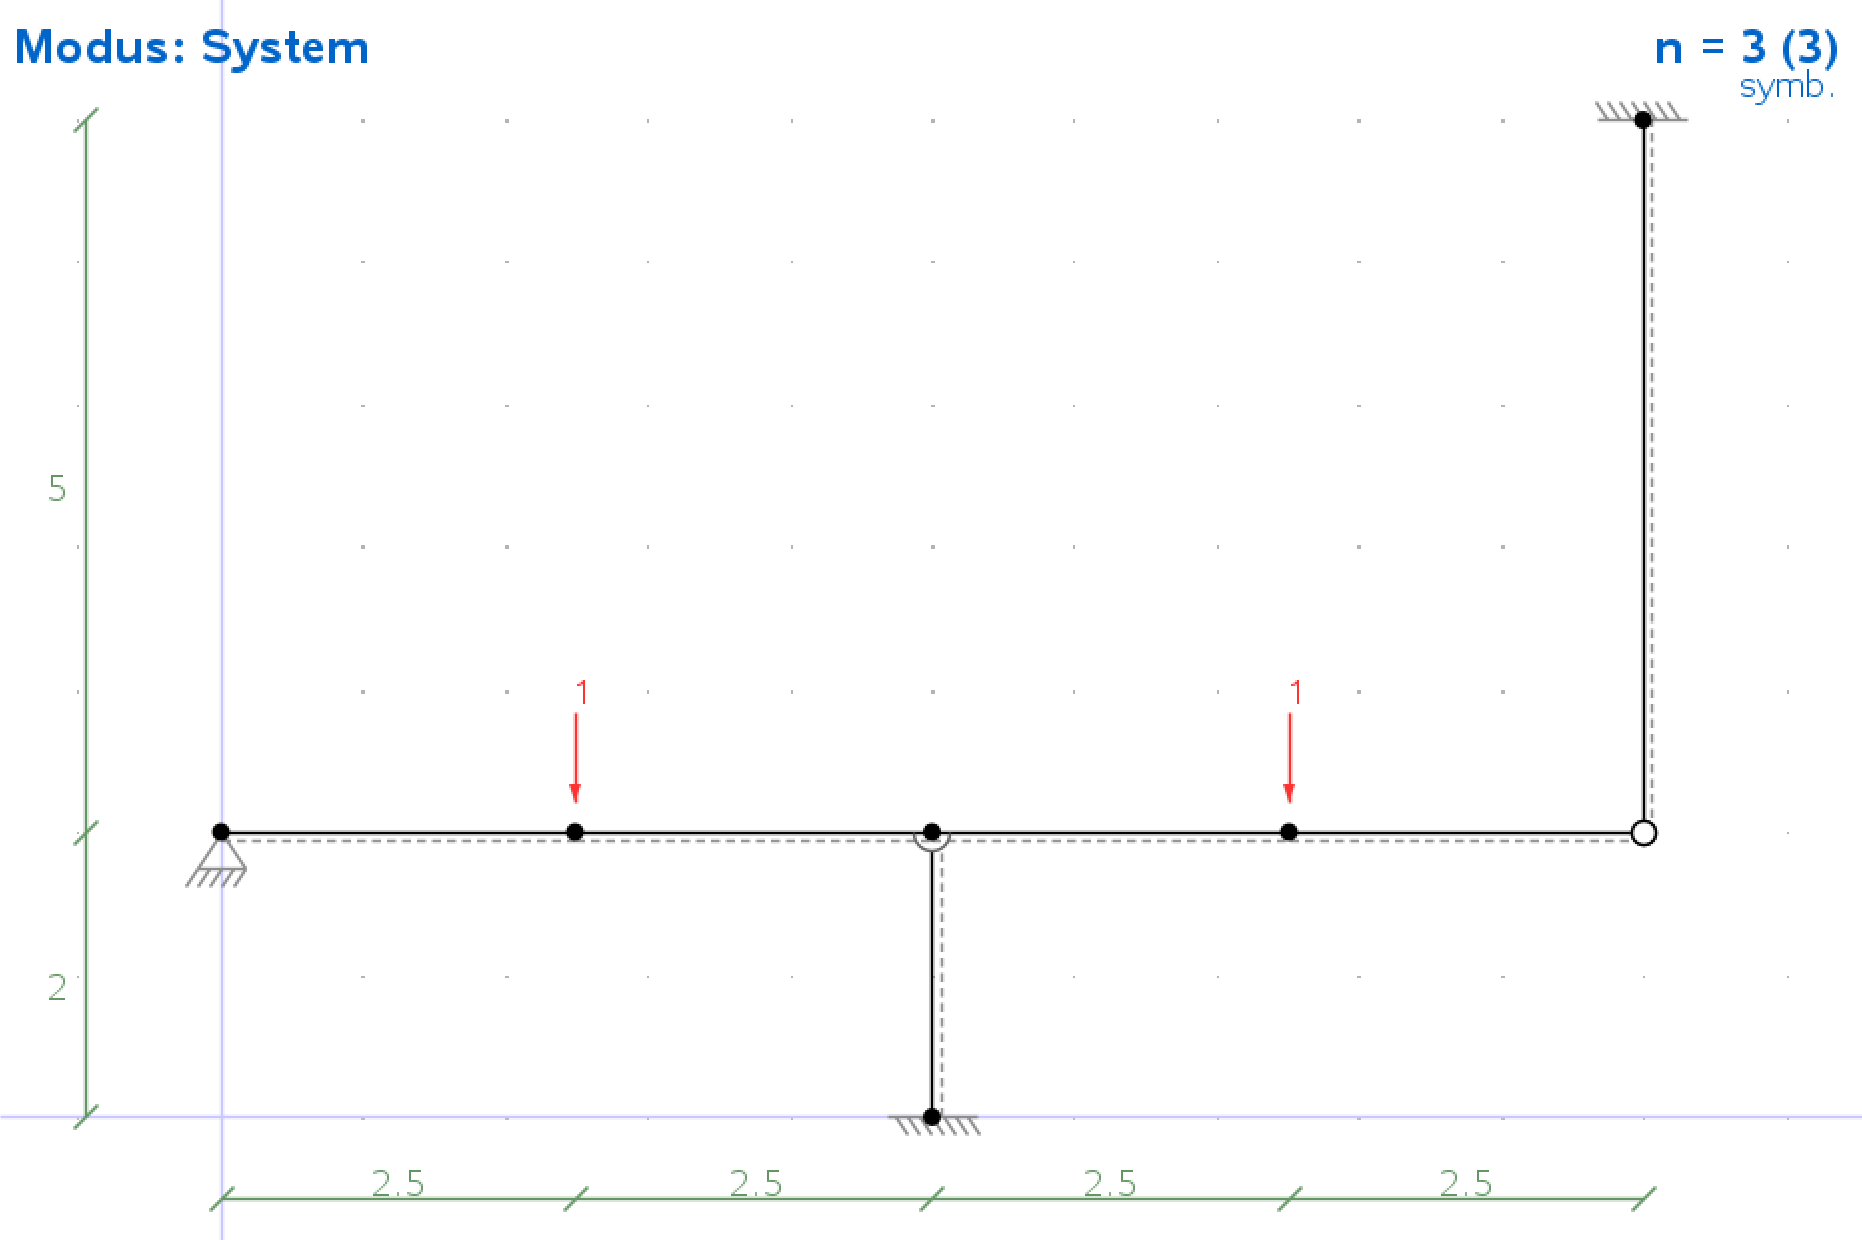
\includegraphics[width=0.5\linewidth]{./fig/TM2/WiSe2021nr4_1.png}
    \caption{TM2 WiSe~20/21, Nr.~4a im Programm}
    \label{fig:verschiebungSystem}
\end{figure}

In den \emph{neuen} Exportfunktionen wird die Temperatur auch symbolisch miteinberechnet.
Um also ann die Verschiebung des rechten unteren Knoten zu kommen lässt sich das entweder über die obere
Knotenexportfunktion machen, über die Biegelinie des rechten horizontalen Stabes oder über die Längsverschiebungsfunktion
des rechten vertikalen Stabes. Über den CAS Befehl \code{solve()} lässt sich die Temperatur direkt ausrechnen 
(vgl. Abb.~\ref{fig:verschiebungErgebniss}). Ich habe hier die Tempertur $dt$ genant (nur $T$ ist wie bereits erwähnt nicht erlaubt),
die Variable nach der aufgelöst werden soll muss der \code{solve()} Funktion als zweites Argument mit gegeben werden.

\begin{figure}[htbp]
    \centering
    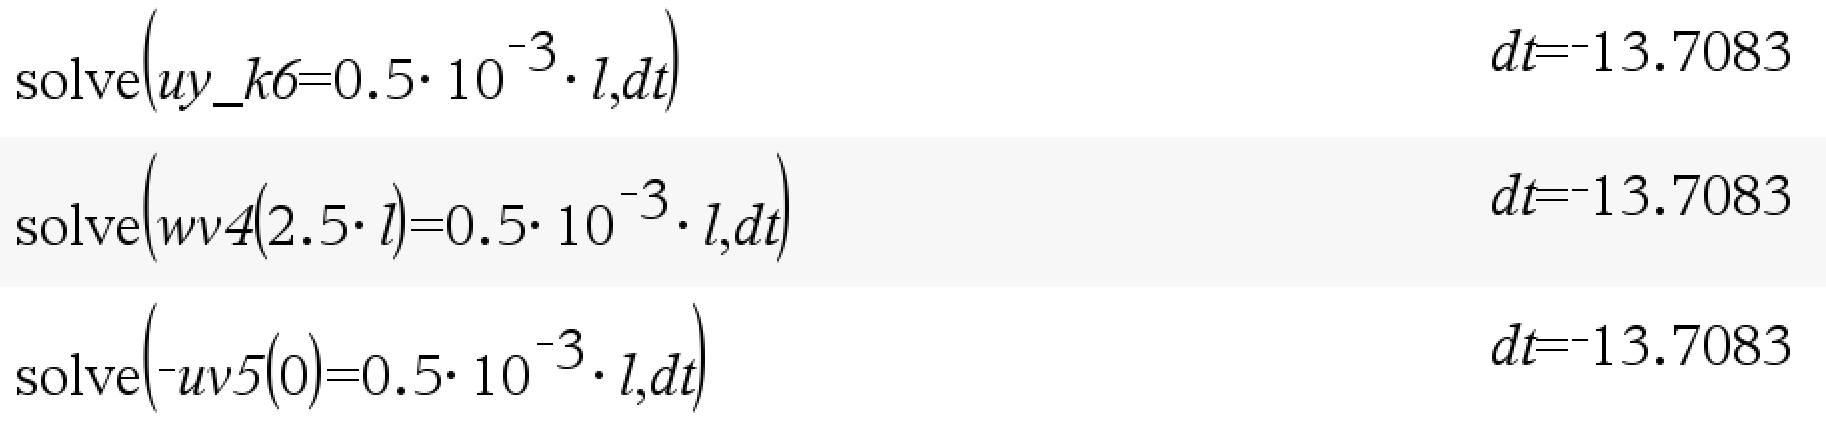
\includegraphics[width=0.5\linewidth]{./fig/TM2/WiSe2021nr4_2.png}
    \caption{Lösung von TM2 WiSe~20/21, Nr.~4a}
    \label{fig:verschiebungErgebniss}
\end{figure}

Der Zweite Teil der Aufgabe lässt sich auch im Programm lösen (Abb.~\ref{fig:VerschiebungTemp}), jedoch gibt es auch hier
ein paar Feinheiten. Ein deratiges System zu speichern kann sich lohnen. Auch hier gelten natürlich die gleichen Hinweise zu den Einheiten.

\begin{figure}[htbp]
    \centering
    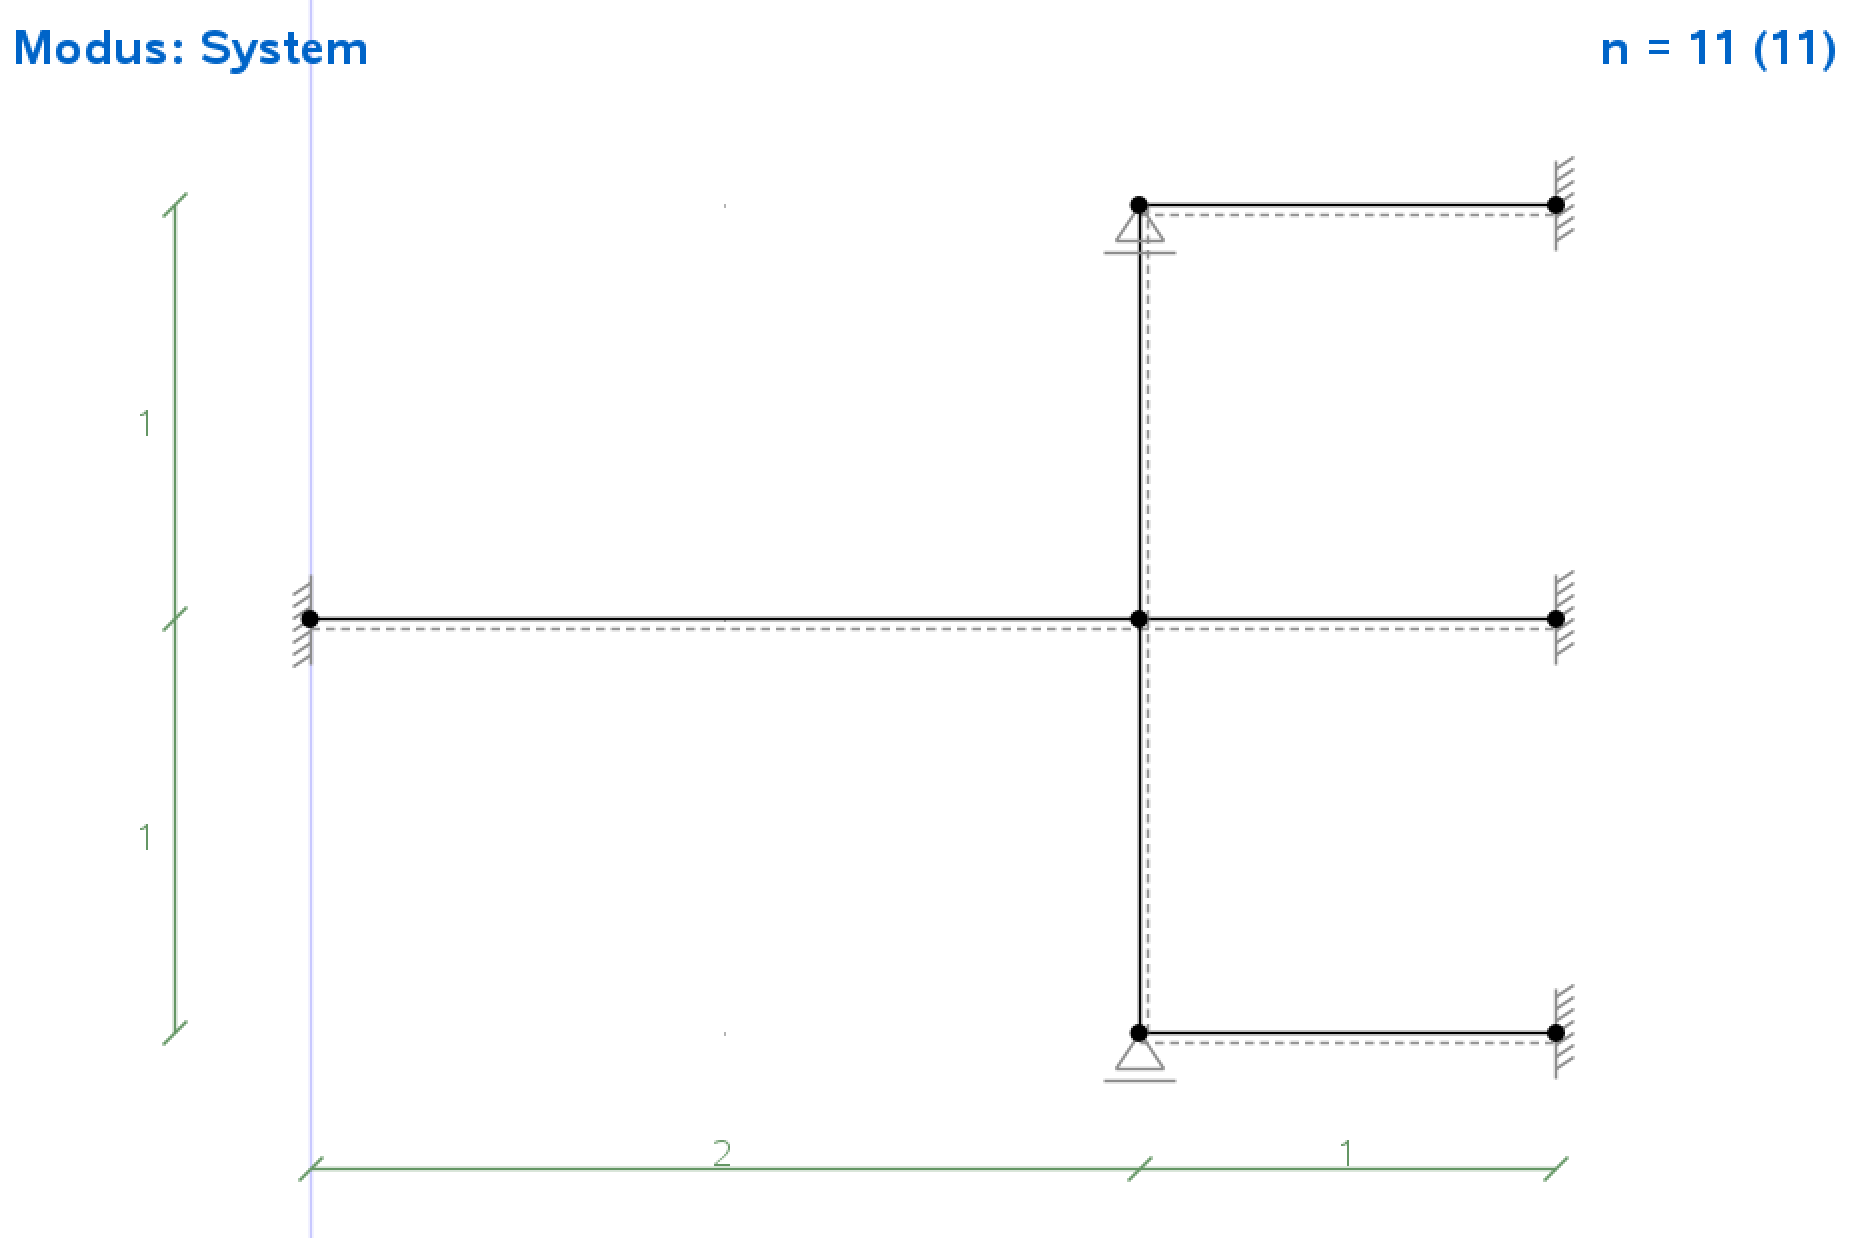
\includegraphics[width=0.5\linewidth]{./fig/TM2/WiSe2021nr4_3.png}
    \caption{TM2 WiSe~20/21, Nr.~4b im Programm}
    \label{fig:VerschiebungTemp}
\end{figure}

Da das Programm nur schnittgrößen direkt berechnet müssen diese noch in Spannungen umgerechnet werden, dafür gibt es in diesem Fall
zwei Möglichkeiten (vgl. Abb.\ref{fig:TM2WiSe2021Nr4b}). Entweder man rechnet die Spannunge direkt über die Schnittkraftverläufe aus,
oder über die Ableitung der Verschiebungsfunktion. Für die zweite Methode muss jedoch darauf geachtet werden den Temperatur Anteil
korrekt zu verrechnen.\\
Erstere Methode ist für Aufgaben mit Zahlenwerten auf jeden Fall die Einfachere, für Aufgaben mit symbolischen Temperatur Werten muss jedoch
die zweite Methode gewählt werden, da die Schnittkraftverläufe diese nicht auf die gewünschte Art berücksichtigen.

\begin{figure}[htbp]
    \centering
    \begin{subfigure}[t]{0.48\textwidth}
        \centering
        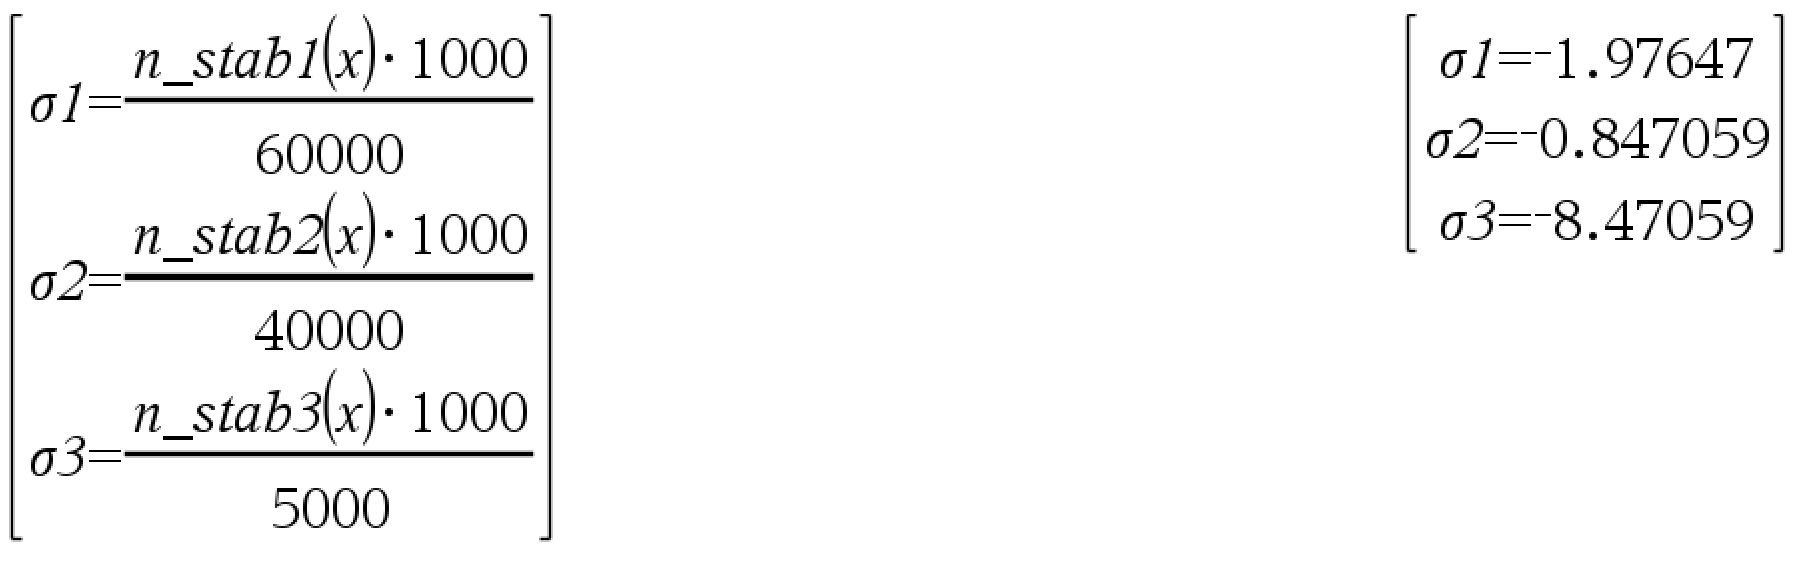
\includegraphics[width=\linewidth]{./fig/TM2/WiSe2021nr4_4.png}
        \caption{Über Schnittgrößen}
    \end{subfigure}
    \hfill
    \begin{subfigure}[t]{0.48\textwidth}
        \centering
        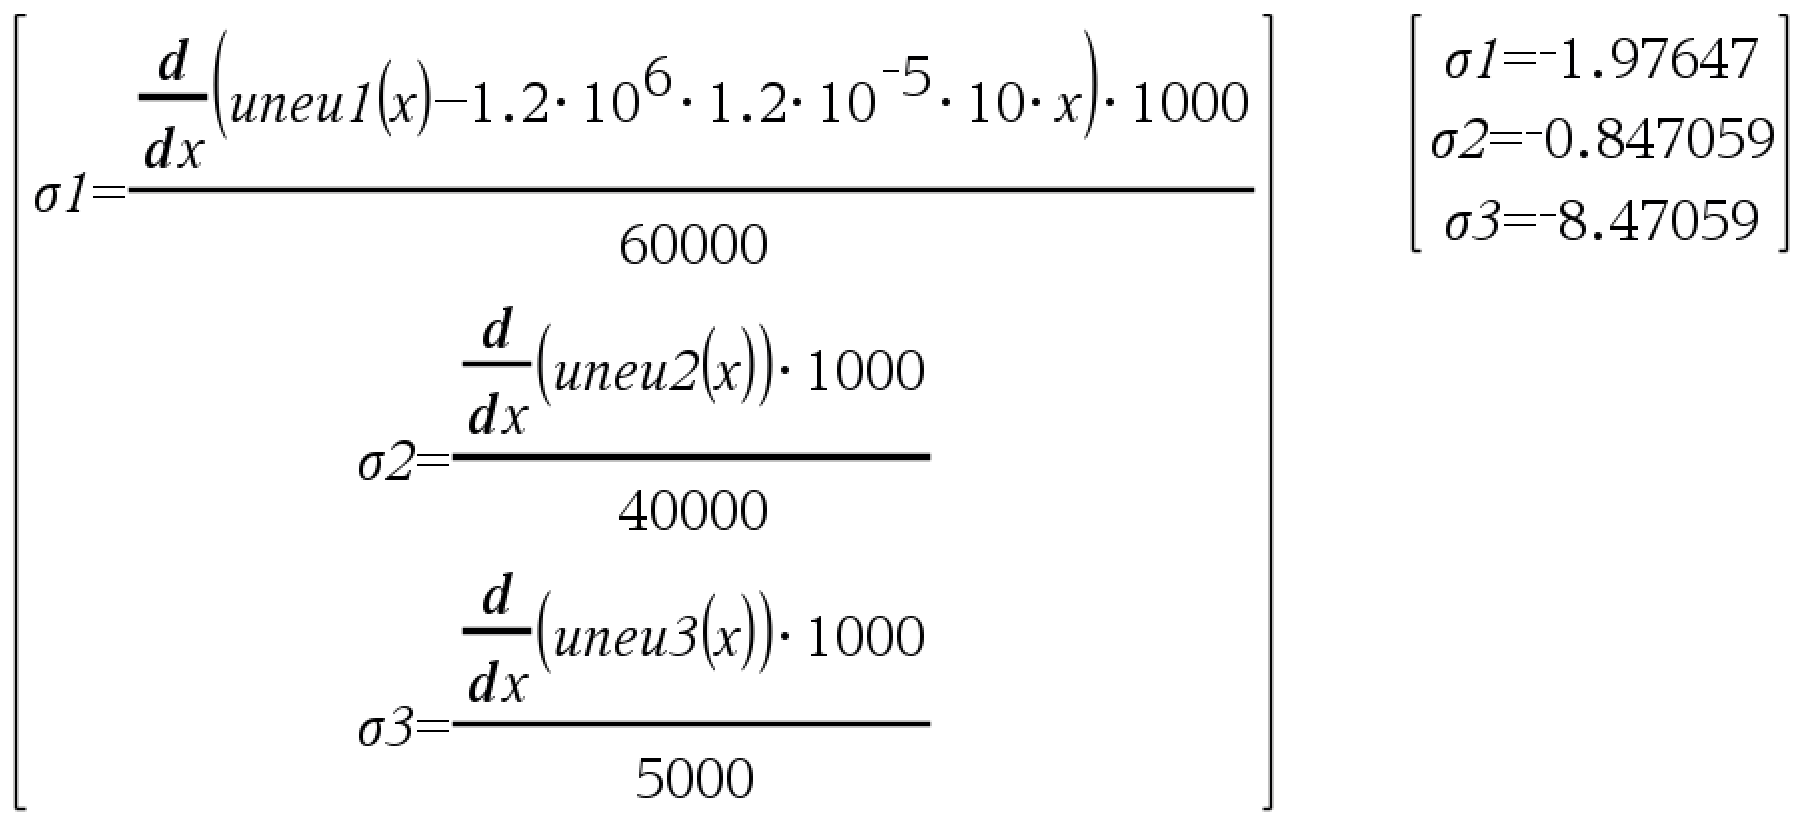
\includegraphics[width=\linewidth]{./fig/TM2/WiSe2021nr4_5.png}
        \caption{Über Verschiebungsfunktion}
    \end{subfigure}
    \caption{Lösung von TM2 WiSe~20/21, Nr.~4b}
    \label{fig:TM2WiSe2021Nr4b}
\end{figure}

Ich will hier anmerken das bei dieser Aufgabenart häufig Hinweise und Warnungen angezeigt werden. Wie z.B. hier auch bei Teilaufgabe a) eine Warnung
zur symbolischen Temperatur. Diese Warnungen sind zwar so konzipiert, dass sie nur angezeigt werden wenn das Programm bzw. ich denke
das etwas falsch eingegeben wurde, jedoch ist es schwer dabei zu vermeiden das auch bei richtiger Eingabe nie eine Warnung oder Hinweis kommt.
Aus diesem Grund empfehele ich, wenn nicht direkt ersichlich ist warum eine Warnung kommt die komplette Eingabe nochmal zu prüfen,
falls diese aber wirklicht korrekt ist sollten auch die Ergebnisse stimmen.


\subsection{Pendelstabannahme (TM2 WiSe 22/23 Nr.~4)} \label{ex:Pendelstabannahme}

\begin{figure}[htbp]
    \centering
    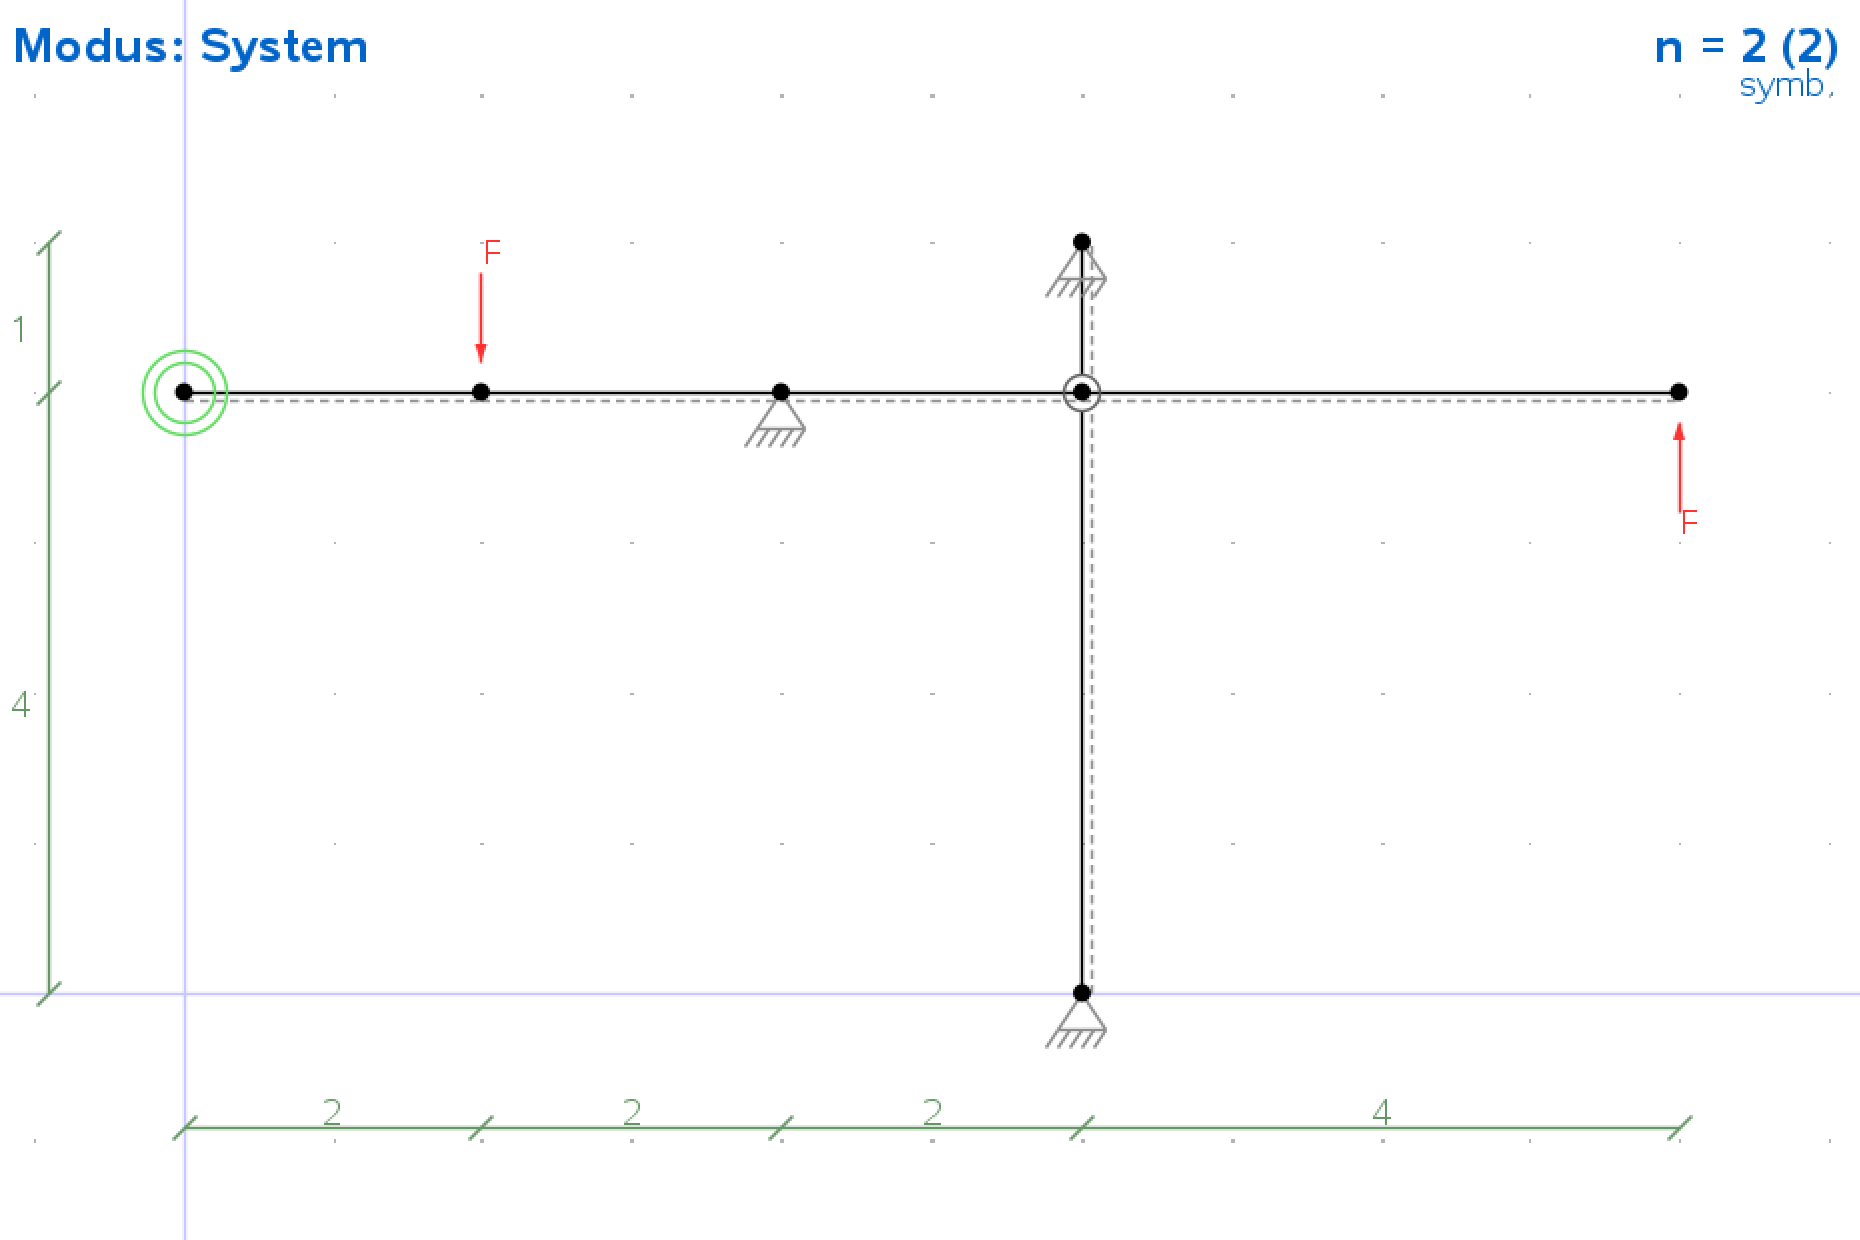
\includegraphics[width=0.7\linewidth]{./fig/TM2/WiSe2223nr4_1.png}
    \caption{TM2 WiSe~22/23, Nr.~4 im Programm}
    \label{fig:Pendelstabsnnahme}
\end{figure}

Wie die Überschrifft vielleicht bereits vermuten lässt muss bei dieser Aufgabe eine Annahme getroffen werden,
die der Zeichnung strenggenommen wiederspricht. Die beiden vertikalen stäbe sollten eigentlich mit einem Angelenk
an den starren Stab angeschlossen werden.\\
Bei einer Handrechnung wird diese Annahme quasi automatisch getroffen, das Programm macht sowas natürlich nicht automatisch.
Um diese Aufgabe mit dem Programm also korrekt zu rechnen müsseb bei den beiden vertikalen stäbe jeweils Angelenke eingebaut werden.
Falls man das nicht macht wirft das Programm eine Warnung bzw. einen Hinweis.

Bei dieser Aufgabe lassen sich die Ergebnisse entweder aus der Ansicht zur Normalkraft 
oder aus dem E-Modus holen (Abb.~\ref{fig:TM2WiSe2223Nr4}).

\begin{figure}[htbp]
    \centering
    \begin{subfigure}[t]{0.48\textwidth}
        \centering
        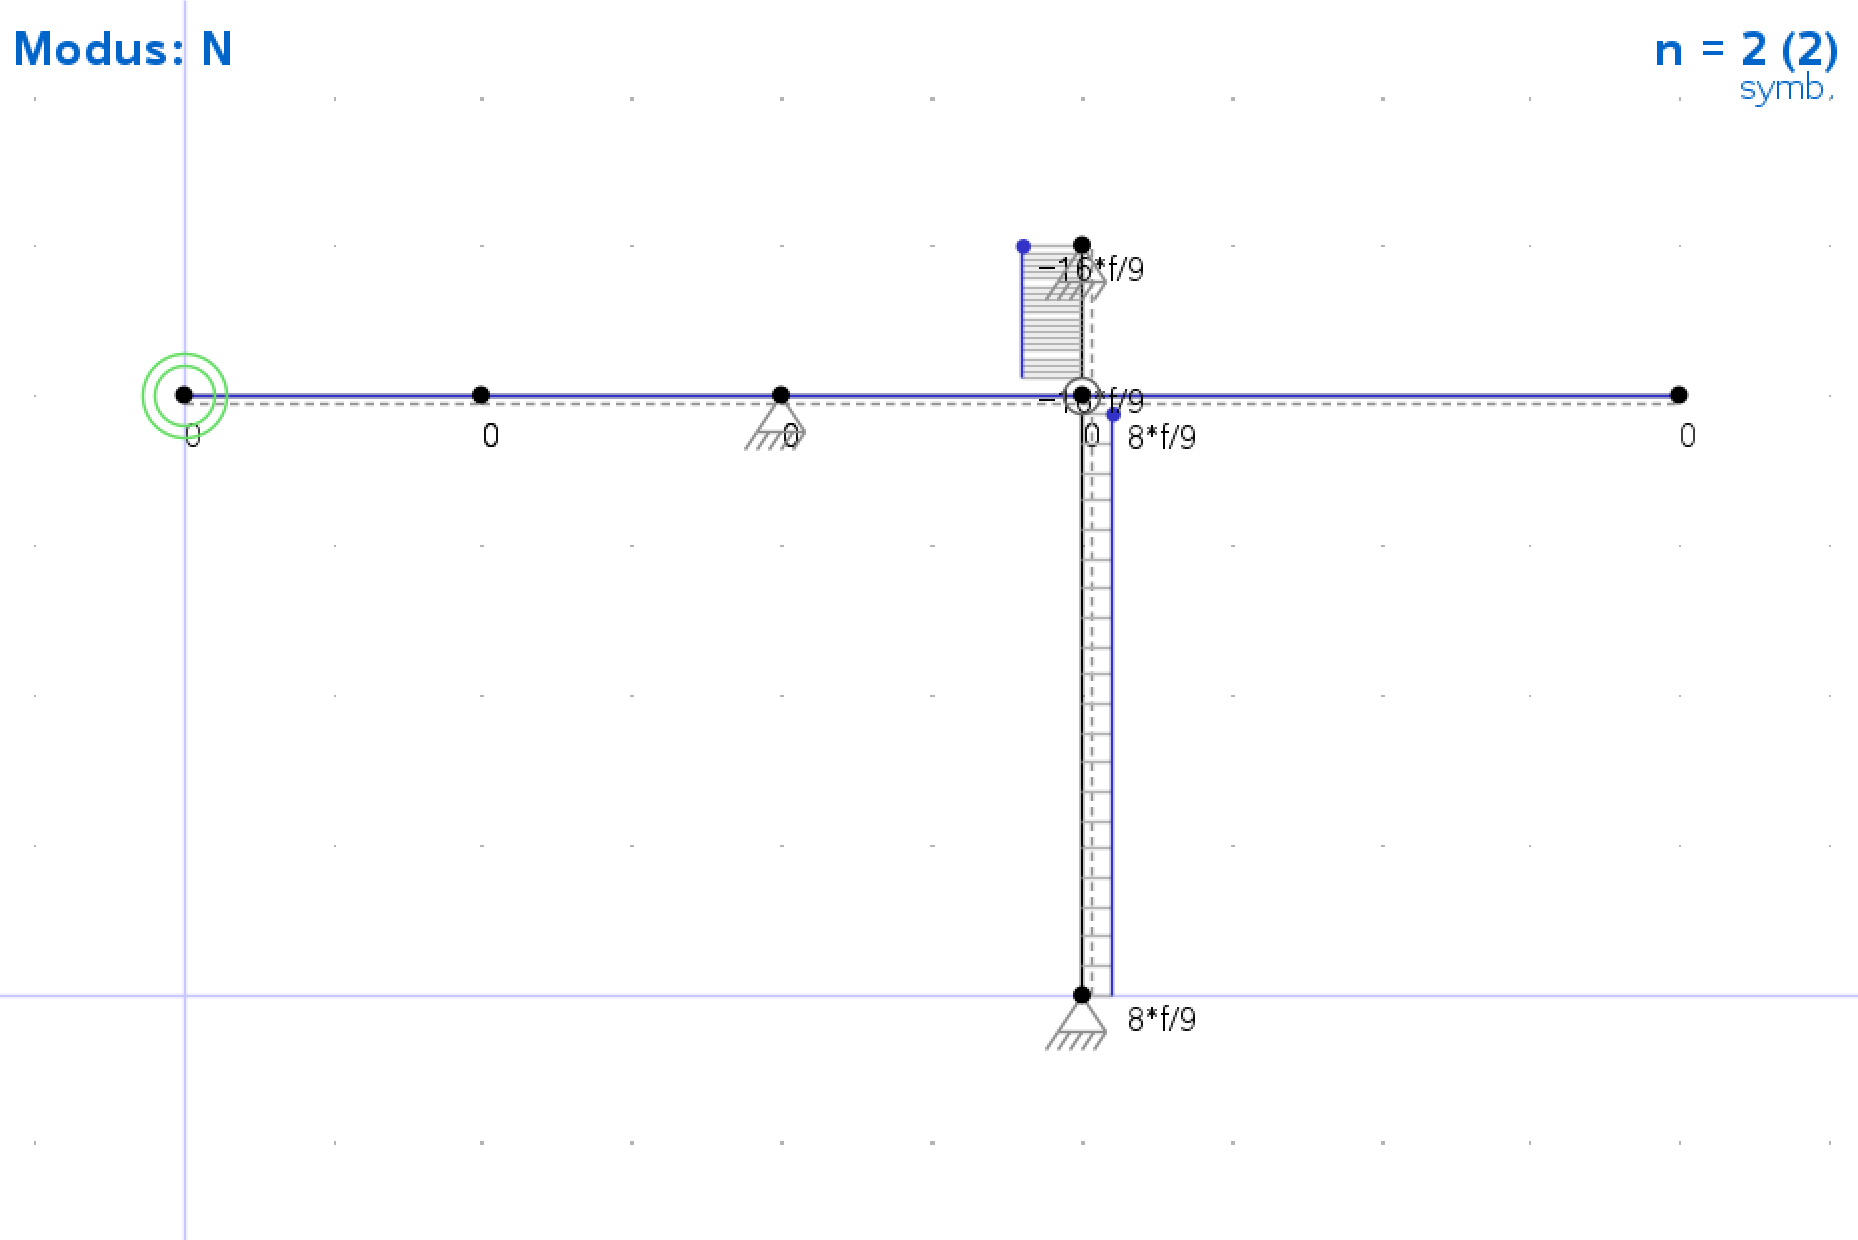
\includegraphics[width=\linewidth]{./fig/TM2/WiSe2223nr4_2.png}
        \caption{Normalkraft}
    \end{subfigure}
    \hfill
    \begin{subfigure}[t]{0.48\textwidth}
        \centering
        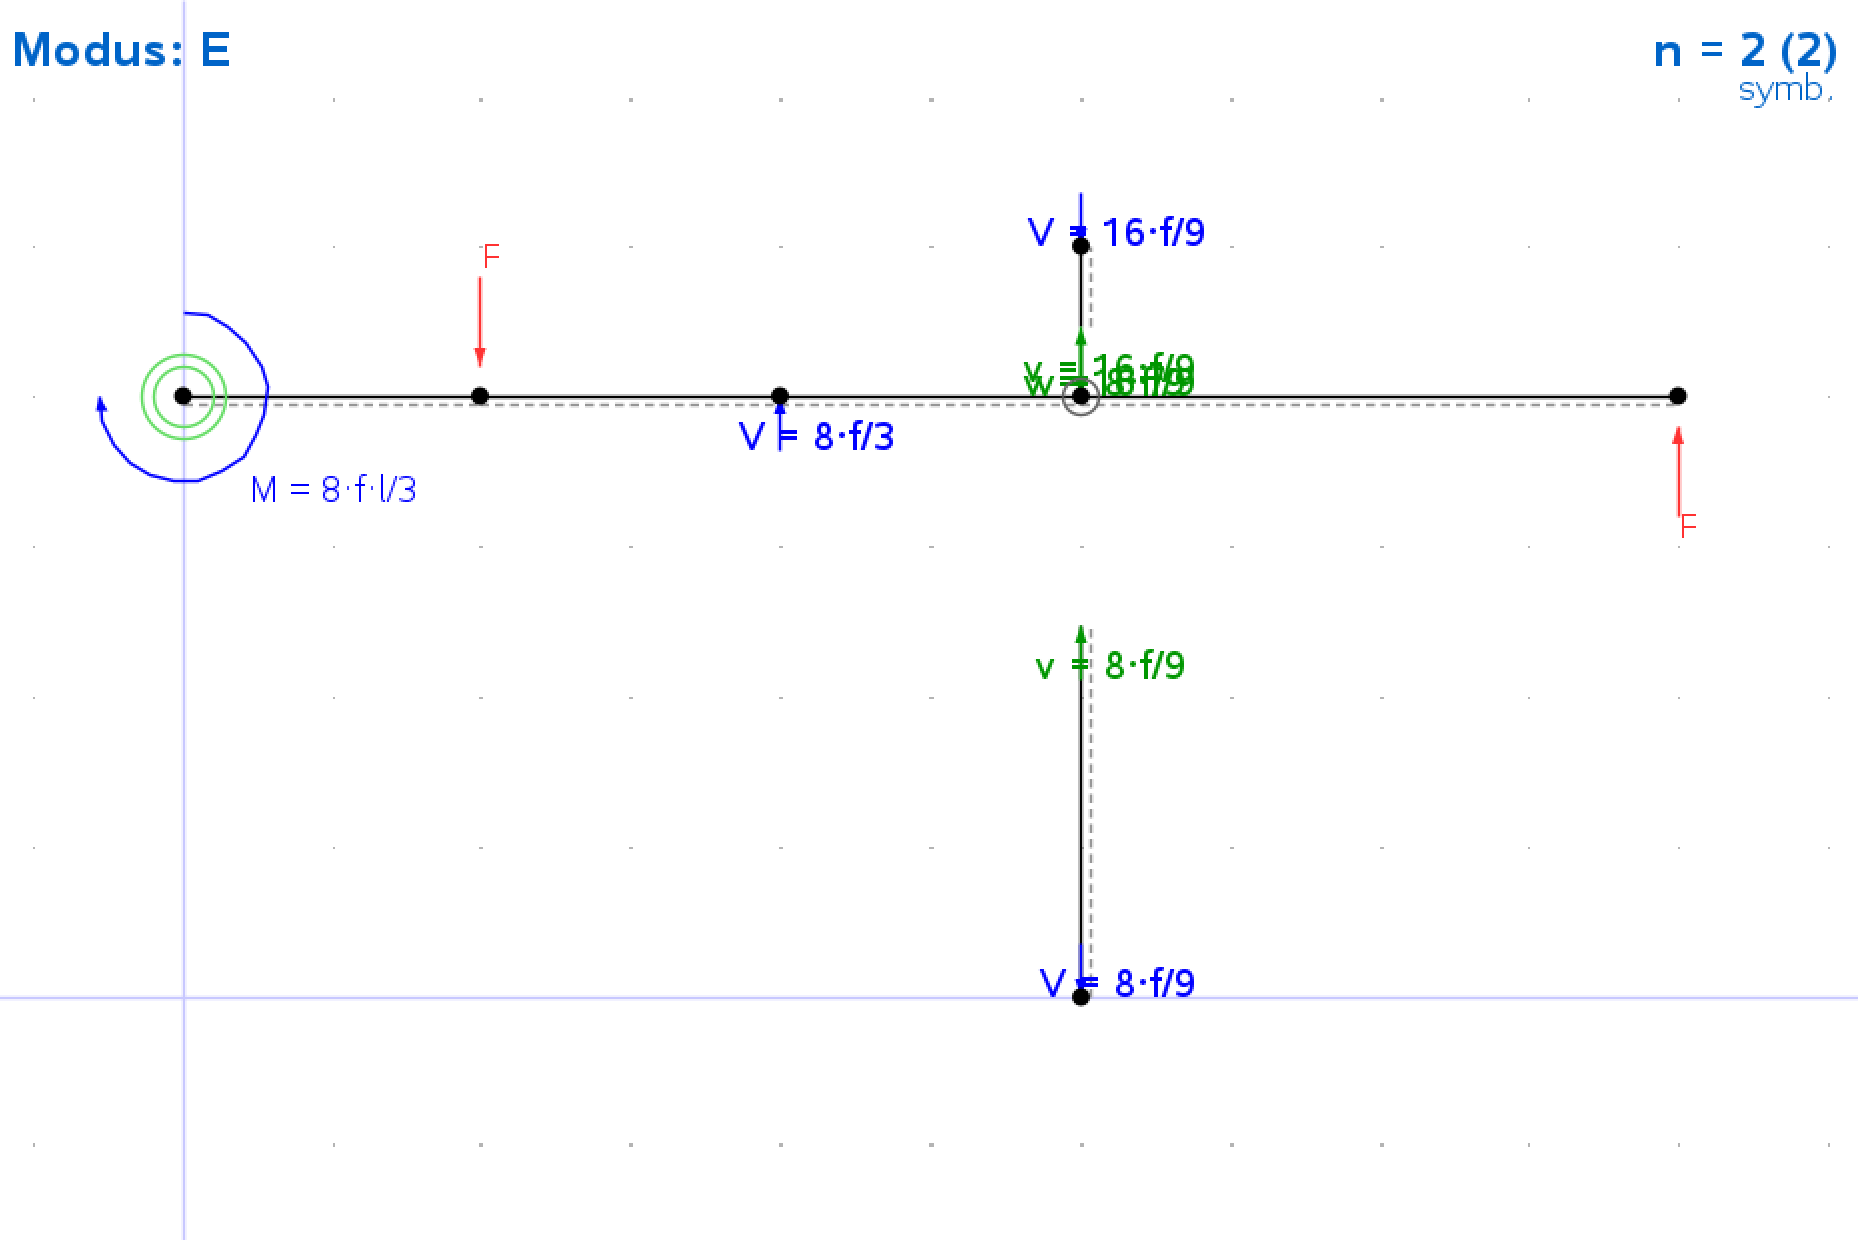
\includegraphics[width=\linewidth]{./fig/TM2/WiSe2223nr4_3.png}
        \caption{E-Modus}
    \end{subfigure}
    \caption{Lösung von TM2 WiSe~22/23, Nr.~4}
    \label{fig:TM2WiSe2223Nr4}
\end{figure}

\textbf{Wichtig} ist, dass das Programm, für symbolische Federn in den Verläufen in seltenen Fällen nicht die richtigen 
Werte ausgibt (Bei symbolischen Temperaturen sowieso nicht).
Zur Sicherheit würde ich deswegen die Schnittgrößen über die \emph{neuen} Verschiebungsfunktionen ermitteln. 
Das dauert zwar gerade für große Systeme länger, ist aber zuverlässiger weil dort wirklich alles symbolisch gerechnet wird 
und eben nicht gepfuscht wird.



\subsection{Schiefe Biegung (TM2 WiSe 25/26 Nr.~8)}

In dieser Aufgbabe sind die Dicken der dünnwandigen Elemente nicht gegeben, da diese abber sowohl für das
FTM als auch für die Lange des Schwerpunkts wichtig sind, müssen diese Werte manuell mit den Werten aus der 
Aufgabenstellung überschrieben werden. Das geht im Obermenue (Taste \taste{o}) auf Seite 3.\\
Für das Zeichnen so eines schiefen Querschnitts empfielt sich ein Rastermaß von z.B. $\frac{1}{\sqrt{2}}$.

\begin{figure}[htbp]
    \centering
    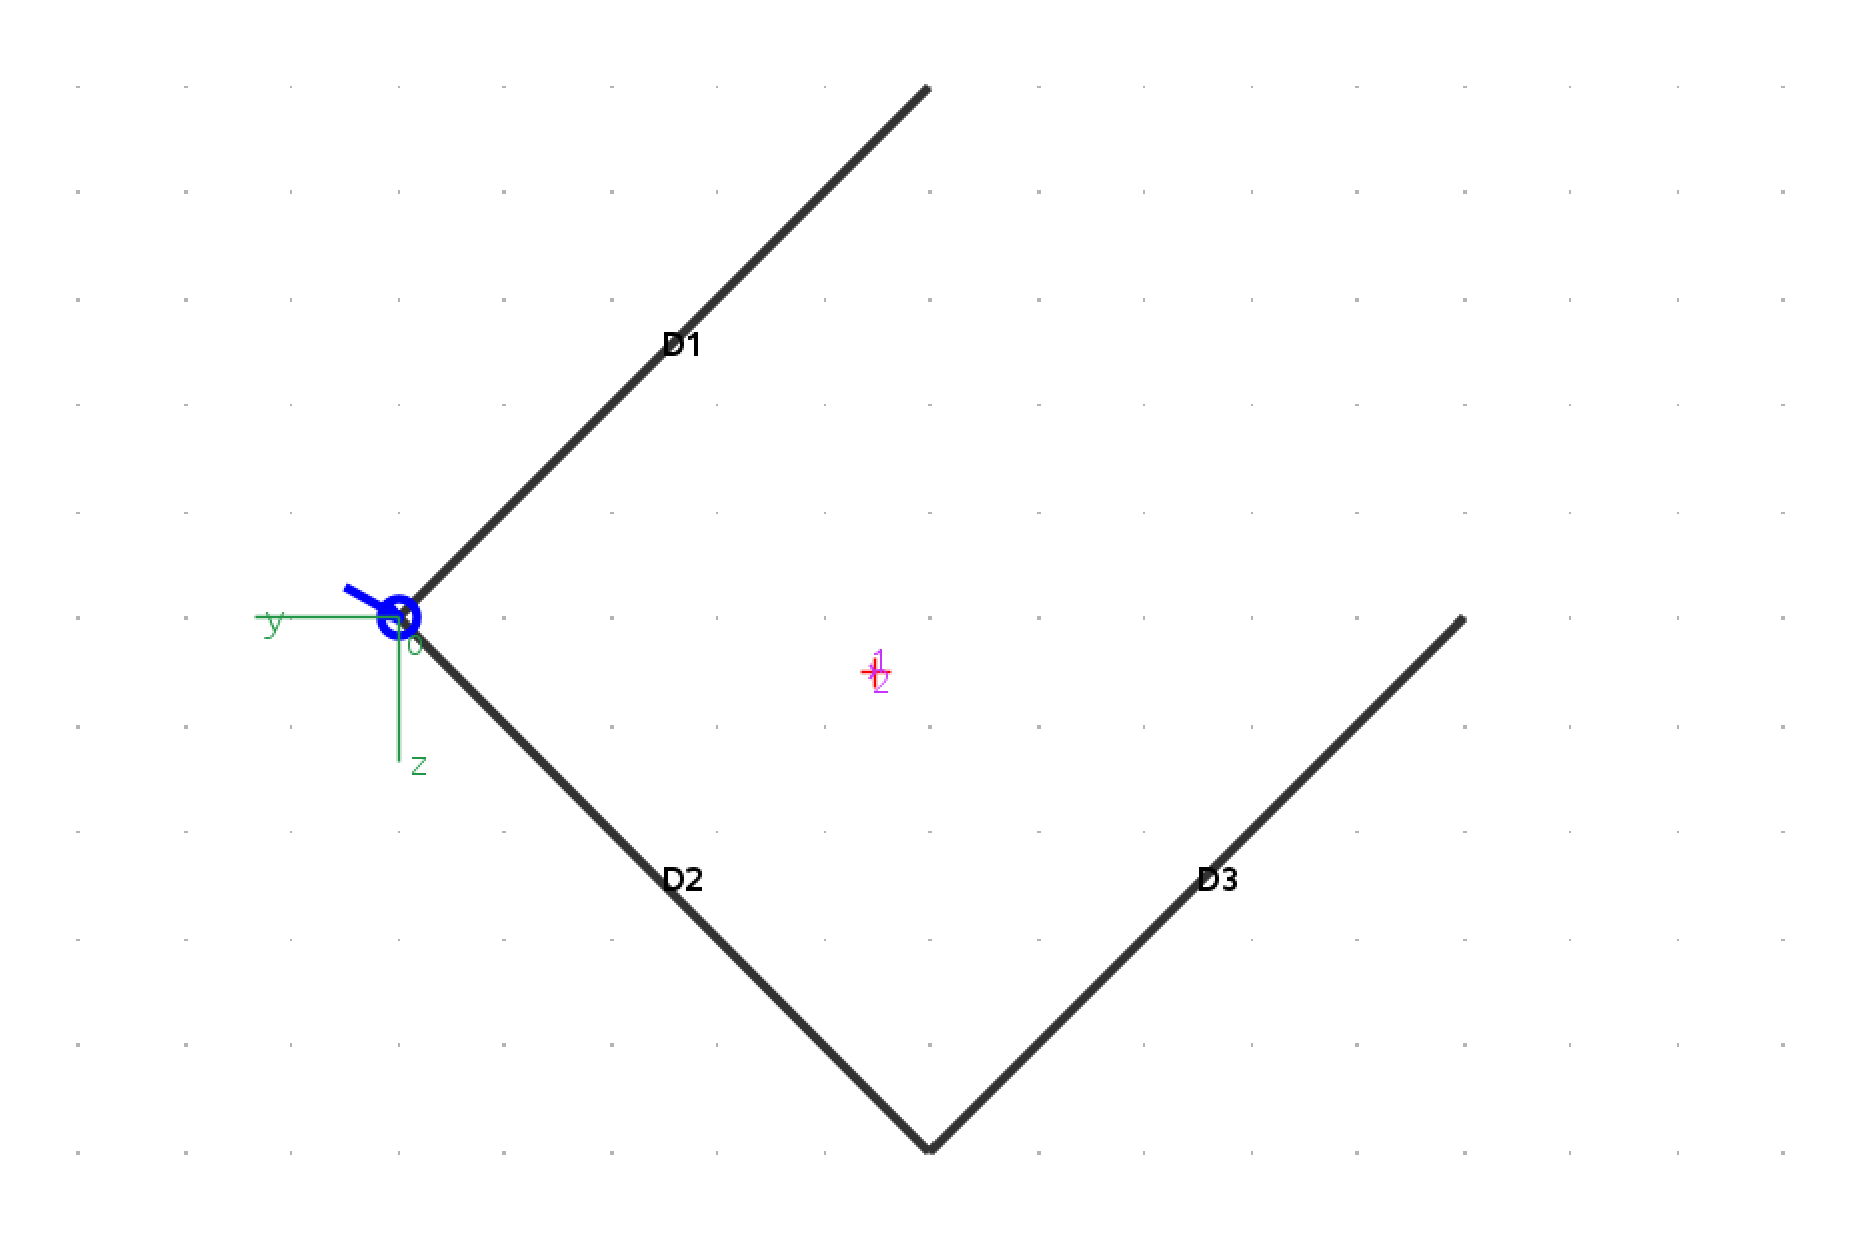
\includegraphics[width=0.7\linewidth]{./fig/TM2/WiSe2526nr8_1.png}
    \caption{TM2 WiSe~25/26, Nr.~8 im Programm}
    \label{fig:TM2WiSe2526Nr8_1}
\end{figure}

Bei dieser Aufgabe braucht man die $\sigma_x$-Berechnung. Um die Normalkraft hier richtig einzuberechnen
muss die Resultierende der Streckenlast über die halbe Länge berechnet werden, also: 
$R=0,1~\frac{\text{kN}}{cm}\cdot100~\text{cm}$.
Für die Kraft muss also $F_y=-500~\text{N}$, $F_z=300~\text{N}$ und $F_x=10000~\text{N}$ eingegeben werden.

Nach dem Aufruf der Berechnung werden noch ein paar Werte abgefragt. Für die ersten Drei muss Null eingetragen werden.
Man hätte auch keine Kraft platzieren können, die Normalkraft und Momente handisch ausrechnen können und diese dann in diese Felder eintragen können.
Das Ergebniss ist das gleiche.\\
Für $\Delta x$ muss $100~\text{cm}$ eingetragen werden, das ist der Abstand zwischen dem gezeichneten Schnitt und dem betrachteten Schnitt.
Das Programm rechnet dann also automatisch die Momente aus der Querkraft aus. Dieses Feature funktioniert natürlich nur, wenn zwischen dem gezeichneten und berechneten Schnitt
keine Weiteren Einflüsse wie Lager oder Kräfte Angreiffen, dann kommt man nicht darum herum $N$, $M_y$ und $M_z$ händisch auszurechnen und einzutragen.

Die Ergebnisse sind in Abbildung \ref{fig:TM2WiSe2526Nr8_2} dargestellt.

\begin{figure}[htbp]
    \centering
    \begin{subfigure}[t]{0.48\textwidth}
        \centering
        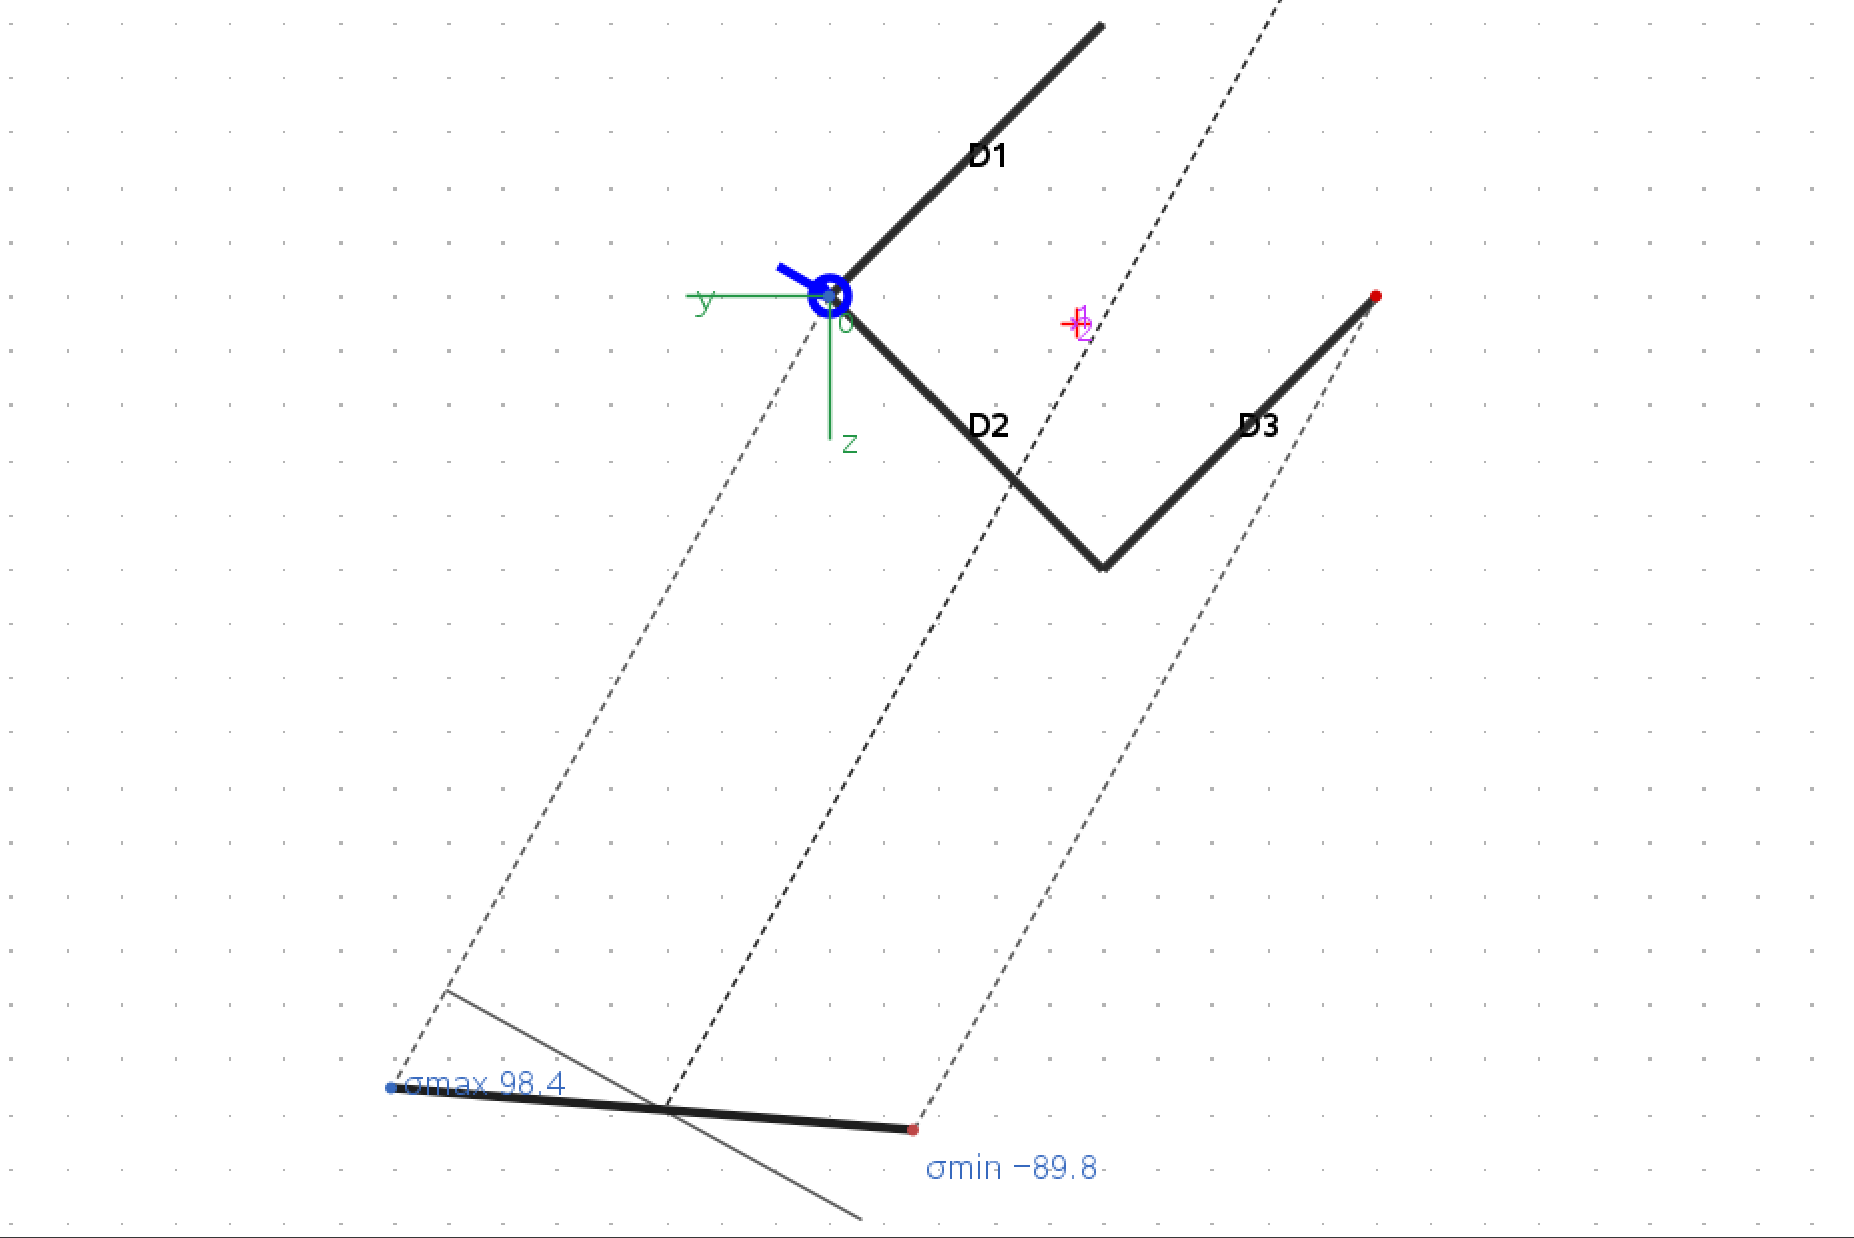
\includegraphics[width=\linewidth]{./fig/TM2/WiSe2526nr8_2.png}
        \caption{Spannungsverlauf}
    \end{subfigure}
    \hfill
    \begin{subfigure}[t]{0.48\textwidth}
        \centering
        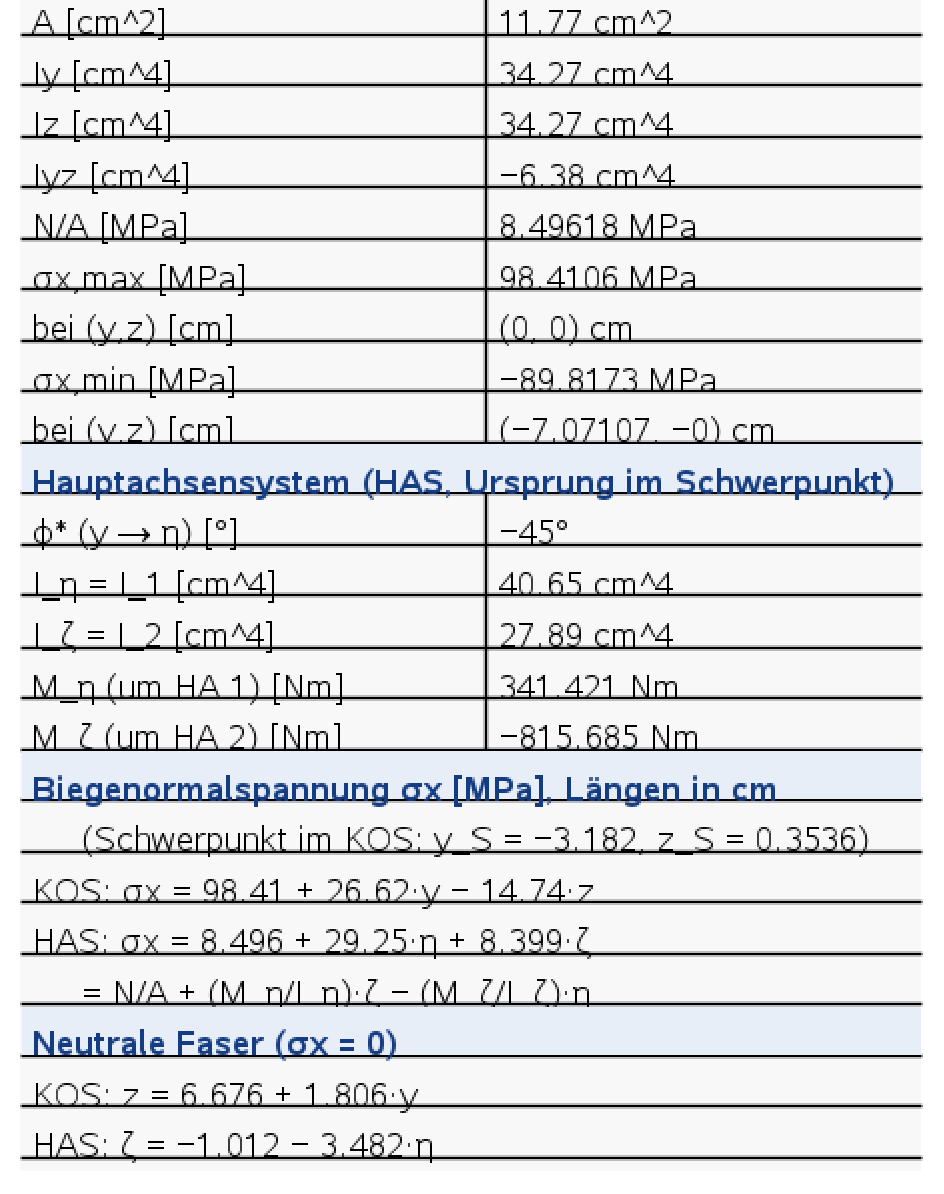
\includegraphics[width=\linewidth]{./fig/TM2/WiSe2526nr8_3.png}
        \caption{Tabellen übersicht}
    \end{subfigure}
    \caption{Lösung von TM2 WiSe~25/26, Nr.~8}
    \label{fig:TM2WiSe2526Nr8_2}
\end{figure}

Ich will anmereken, dass des öfteren bei Aufgaben Querschnittswerte gegeben sind, die nicht zur Bemaßung in der Zeichnung passen,
ob das absichtlich so ist konnte mir leider keiner sagen. Es ist also immer sinnvoll das einmal gegen zu prüfen und die Werte evtl. zu überschreiben.
Was die ISD-Musterlösung bei dieser Aufgabe gerechnet hat, ist mir nicht ganz klar. Meines Verständnisses nach wurde hier mit einem
Schwerpunkt für die Momente aus Normalkraft gerechnet, der genau in der Mitte des U profiels liegt, sodass die Normalkraft um die $y$-Achse kein Moment erzeugt.

\subsection{Schiefe Biegung/Kernfäche (TM2 WiSe21/22 Nr.~8)}



\subsection{MSK (TM2 WiSe 21/22 Nr.~3)}

Zu dieser Aufgabe gibt es eigentlich nicht besonders viel zu sagen, man gibt die gegebenen Werte ein und das Programm
füllt in grün die restlichen Werte auf (Abb.~\ref{fig:TM2WiSe2122Nr3_1}).

\begin{figure}[htbp]
    \centering
    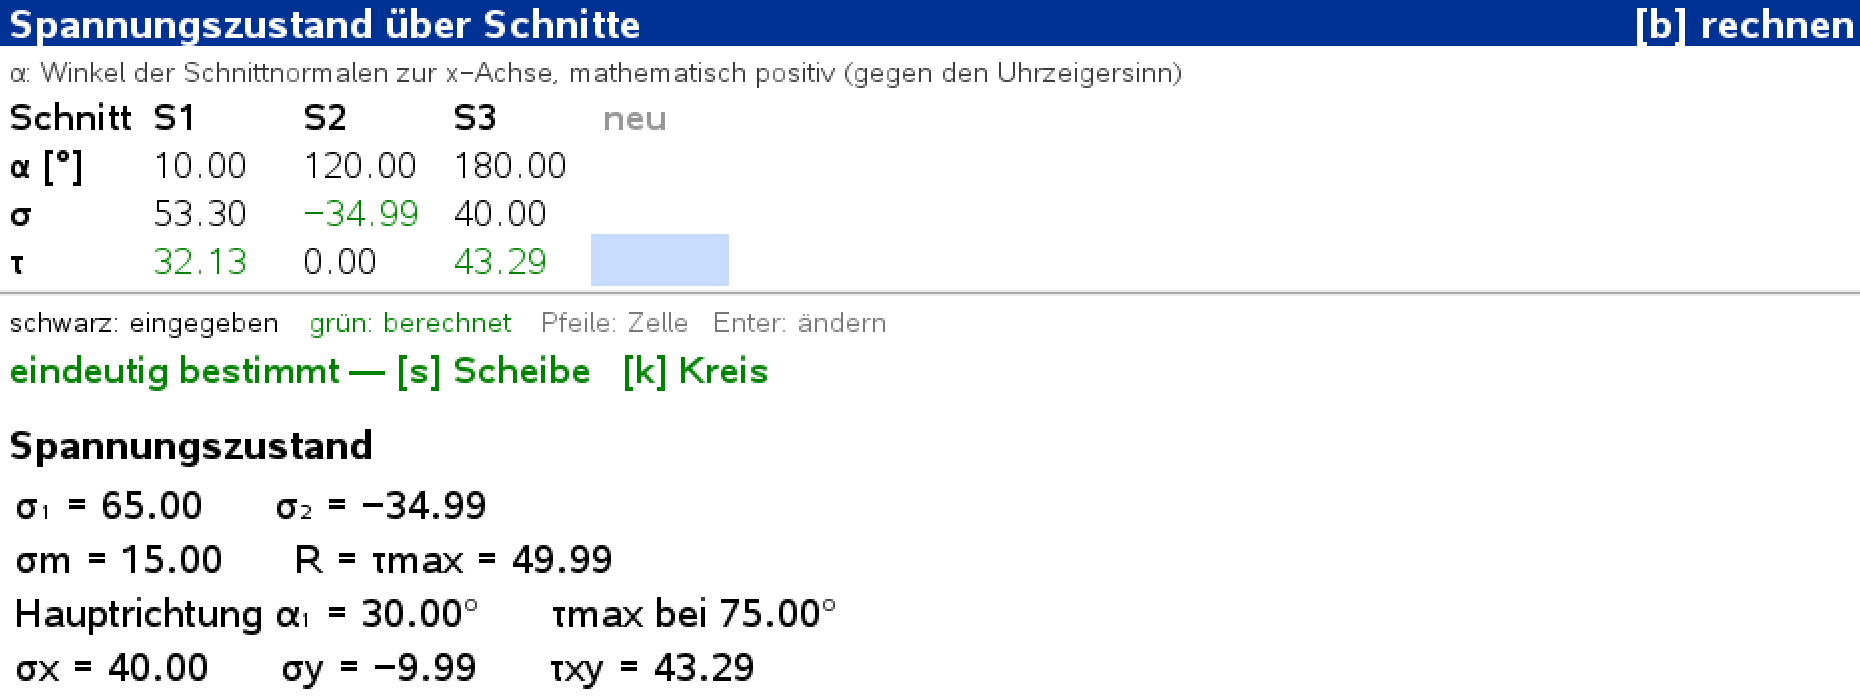
\includegraphics[width=0.7\linewidth]{./fig/TM2/WiSe2122nr3_1.png}
    \caption{TM2 WiSe~21/22, Nr.~3 im Programm}
    \label{fig:TM2WiSe2122Nr3_1}
\end{figure}

Danach bekommt man mit den Tasten \taste{s} und \taste{k} die beiden wichtigen Ansichten (Abb.~\ref{fig:TM2WiSe2122Nr3_2}).


\begin{figure}[htbp]
    \centering
    \begin{subfigure}[t]{0.48\textwidth}
        \centering
        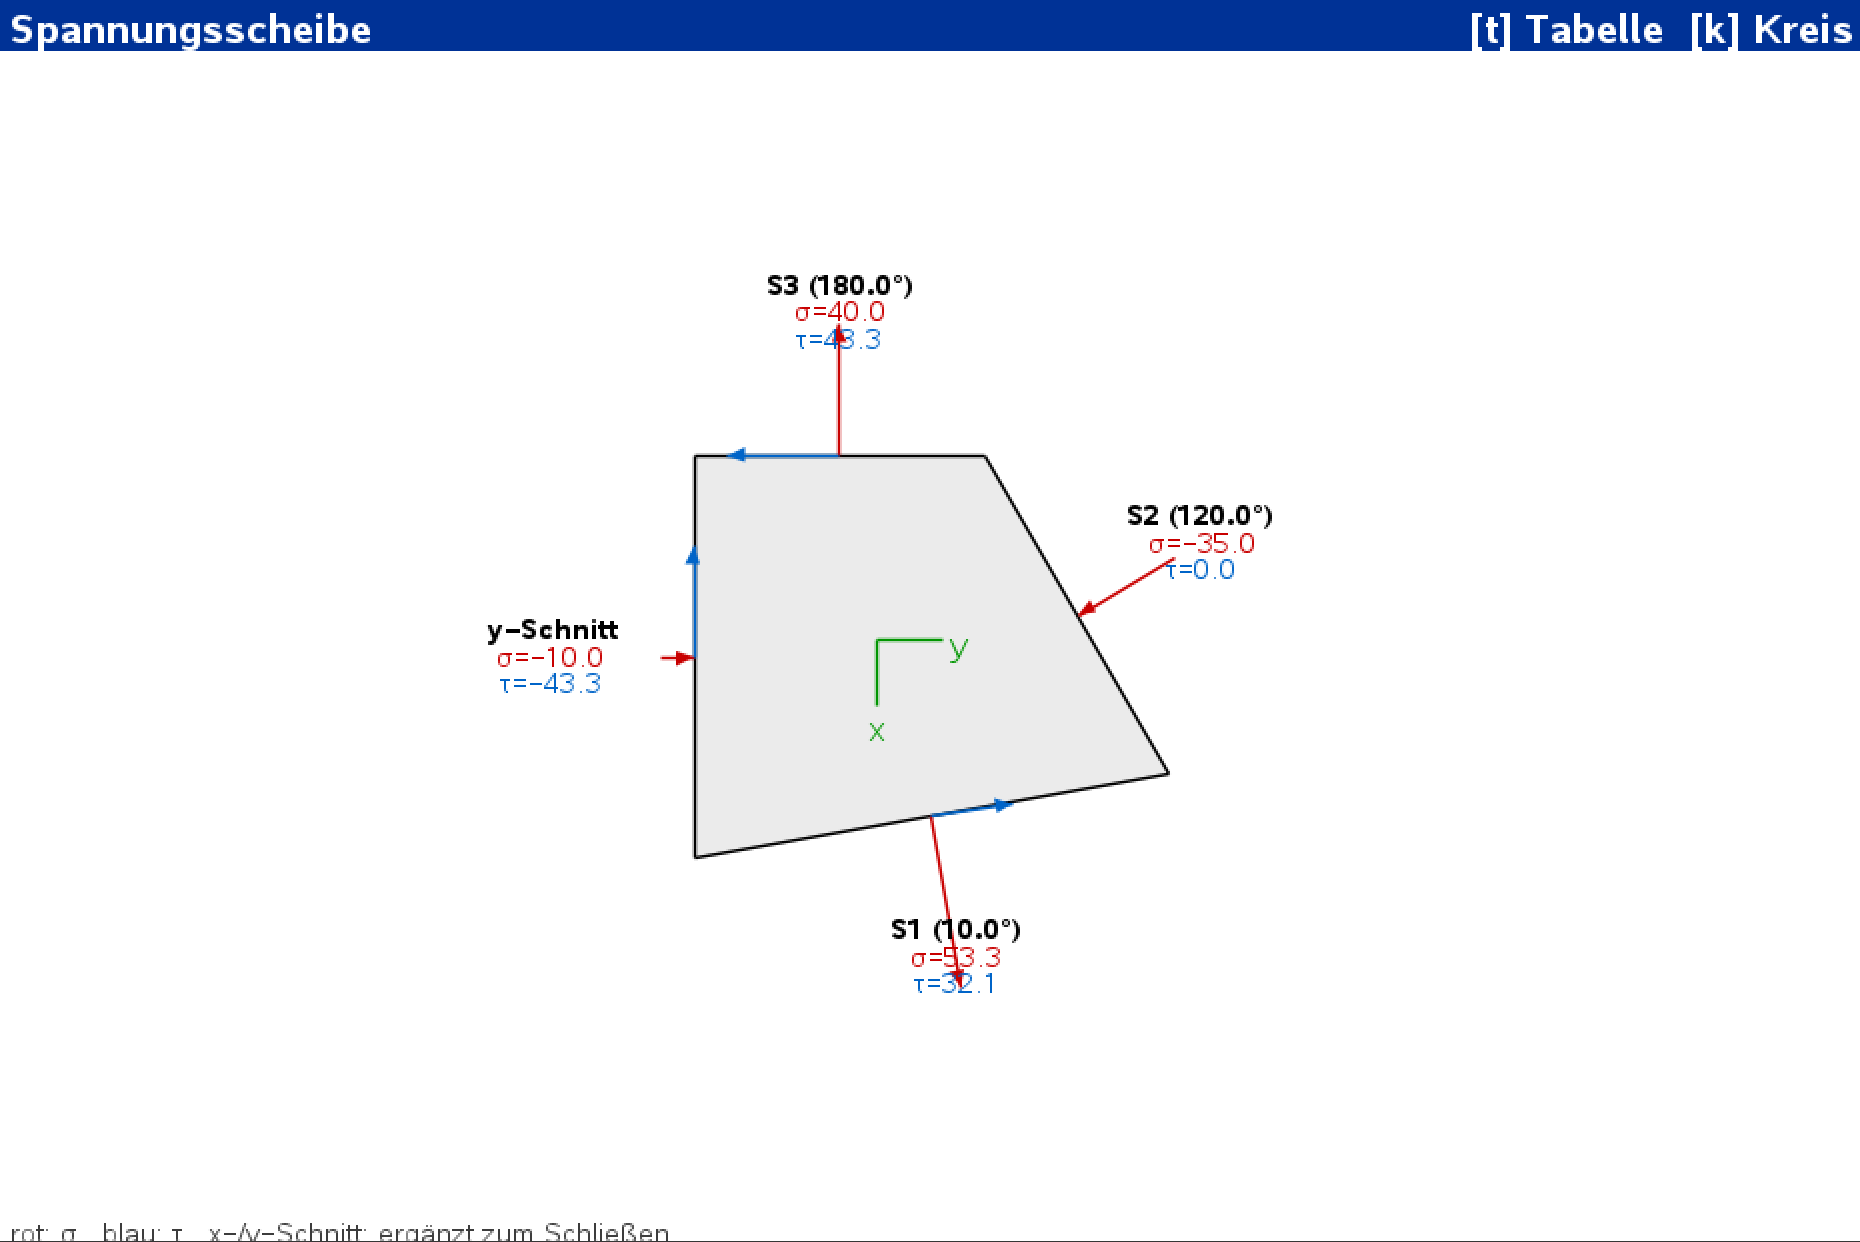
\includegraphics[width=\linewidth]{./fig/TM2/WiSe2122nr3_2.png}
        \caption{Spannungs-Scheibe}
    \end{subfigure}
    \hfill
    \begin{subfigure}[t]{0.48\textwidth}
        \centering
        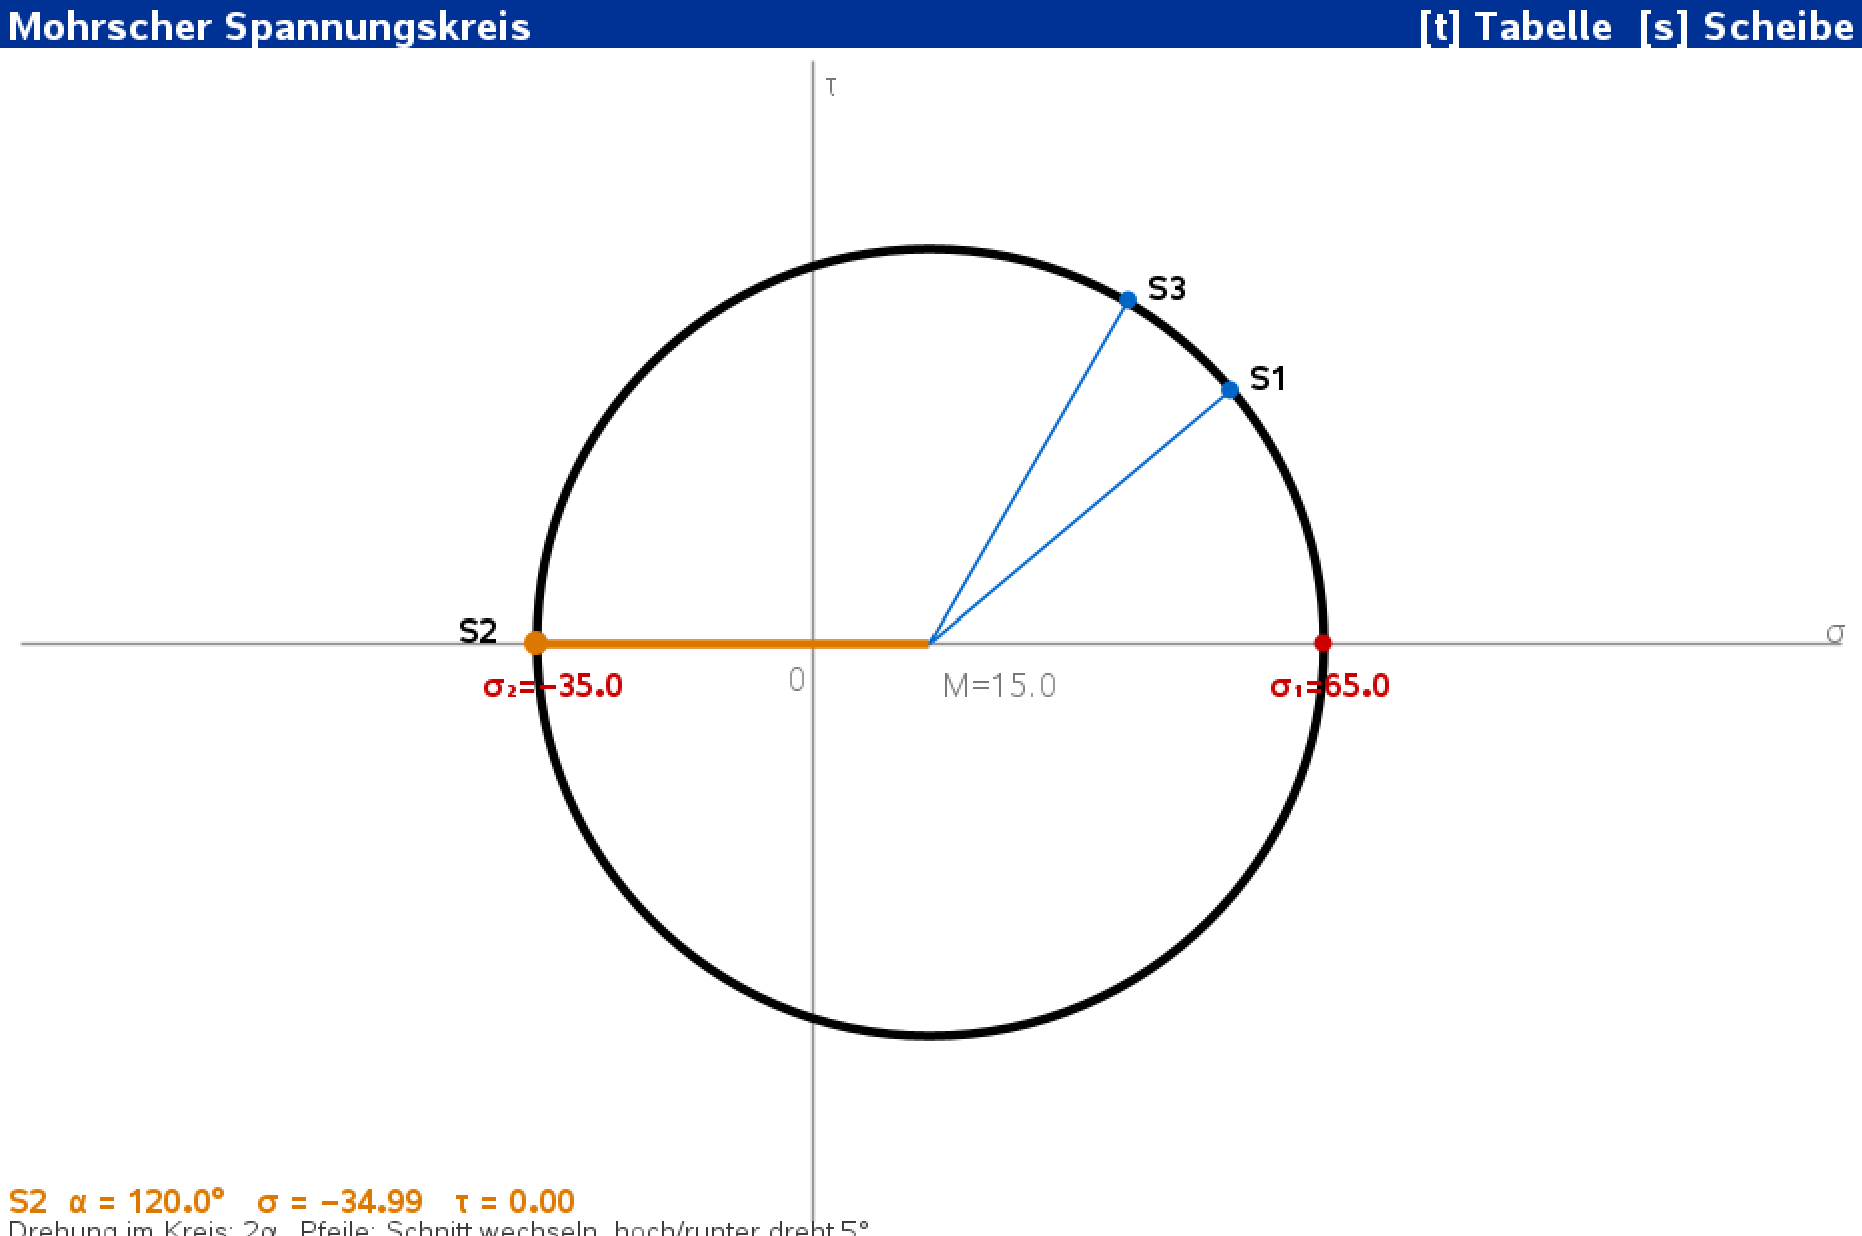
\includegraphics[width=\linewidth]{./fig/TM2/WiSe2122nr3_3.png}
        \caption{Spannungs-Kreis}
    \end{subfigure}
    \caption{Lösung von TM2 WiSe~21/22, Nr.~3}
    \label{fig:TM2WiSe2122Nr3_2}
\end{figure}

Falls bei einer Aufgabe nach dem Winkel eines Schnitts gefragt wird und das Programm zwei Winkel ausgibt, muss natürlich
geprüft werden, welcher Winkel eher zur Skizze passt.

\subsection{Schubspannung und SMP (TM2 SoSe 24 Nr.~8)}

\subsection{Verwölbung (TM2 SoSe 20 Nr.~9)}

%=====================================================================
\appendix
\part{Anhang}

\section{Tastenkürzel Tragwerksskript}

\begin{longtable}{p{0.14\linewidth}p{0.82\linewidth}}
  \toprule
  \textbf{Taste} & \textbf{Funktion} \\
  \midrule \endhead
  \taste{b} & Tragwerk berechnen \\
  \taste{s} & Systemansicht \\
  \taste{n}, \taste{q}, \taste{m} & Normalkraft, Querkraft, Moment \\
  \taste{w}, \taste{u} & Biegelinie, Längsverformung \\
  \taste{e}, \taste{t} & Explosionsansicht, Beschriftungen dort \\
  \taste{v}, \taste{p} & Verschiebungszustand (PvV), Polplan \\
  \taste{l} & Gleichgewichtsbedingungen der Teilsysteme \\
  \taste{o} & Obermenü (Einstellungen und Exporte) \\
  \taste{h} & System einpassen \\
  \taste{f} & Stabrichtung umdrehen \\
  \taste{c}, \taste{ctrl}+\taste{Del} & alles löschen (Rückfrage: \taste{Enter} löscht, \taste{Esc} bricht ab) \\
  \taste{+}, \taste{-} & Zoom \\
  \taste{0}\dots\taste{9} & KGV: Lastzustand (\taste{0}) bzw.\ Einheitszustand wählen (bei Auto-KGV) \\
  \taste{Enter} & Menü öffnen, Wert umschalten, Eingabe übernehmen \\
  \taste{Esc} & Box, Eingabe, Menü oder Modus schließen \\
  \taste{Del} & Zeichen in der Eingabe bzw.\ Element unter dem Zeiger löschen \\
  Pfeiltasten & Ansicht verschieben; im Menü Zeile (hoch/runter) und Seite (links/rechts) wählen \\
  \bottomrule
\end{longtable}

\section{Tastenkürzel Querschnittsskript}

\begin{longtable}{p{0.14\linewidth}p{0.82\linewidth}}
  \toprule
  \textbf{Taste} & \textbf{Funktion} \\
  \midrule \endhead
  \taste{m}, \taste{d} & Massiv- bzw.\ Dünnwandmenü \\
  \taste{b} & Berechnungsmenü \\
  \taste{e}, \taste{t} & Querschnittswerte, Einzelwerte-Tabelle \\
  \taste{v} & Schubverlauf wählen (danach Ziffern \taste{0}\dots\taste{9}) \\
  \taste{k} & Kernflächenmodus weiterschalten \\
  \taste{o} & Optionen (Raster, Dicke, KOS, Einheiten, $\xi$, FTM-Bezug) \\
  \taste{h} & Geometrie einpassen \\
  \taste{c}, \taste{ctrl}+\taste{Del} & alles löschen (Rückfrage: \taste{Enter} löscht, \taste{Esc} bricht ab) \\
  \taste{+}, \taste{-} & Zoom \\
  \taste{Enter} & Menüpunkt wählen, Element bearbeiten, Eingabe übernehmen \\
  \taste{Esc} & Box, Eingabe oder Ansicht schließen; ist nichts mehr offen, verwirft
    \taste{Esc} alle Ergebnisse (Spannungen, Schub, Torsion, Kernfläche) \\
  \taste{Del} & letzten Punkt bzw.\ letztes Element löschen; in Eingabemasken ein Zeichen \\
  \bottomrule
\end{longtable}

\section{Tastenkürzel Spannungskreis}

\begin{longtable}{p{0.14\linewidth}p{0.82\linewidth}}
  \toprule
  \textbf{Taste} & \textbf{Funktion} \\
  \midrule \endhead
  Pfeiltasten & Zelle wählen; im Kreis die Marke bewegen \\
  Ziffer, \code{.}, \code{-} & Eingabe in der Zelle beginnen \\
  \taste{b} & rechnen \\
  \taste{s}, \taste{k} & Spannungsscheibe, Mohrscher Kreis (nur bei eindeutigem Zustand) \\
  \taste{t}, \taste{e} & zurück zur Tabelle \\
  \taste{ctrl}+\taste{Del} & alles löschen (Rückfrage: \taste{Enter} löscht, \taste{Esc} bricht ab) \\
  \taste{Enter} & Zelle öffnen bzw.\ übernehmen \\
  \taste{Del} & Zeichen löschen bzw.\ Zelle leeren \\
  \taste{Tab} & andere Winkellösung (bei zwei Lösungen) \\
  \taste{Esc} & Eingabe abbrechen, sonst zurück zur Tabelle \\
  \bottomrule
\end{longtable}


\section{Häufige Stolpersteine}

\begin{itemize}
  \item \textbf{Gestrichelte Faser:} Sie muss zur Aufgabe passen (bzw.\ auf der Seite liegen, in die
        die $z$-Achse des gegebenen KOS zeigt), sonst stimmen die Vorzeichen nicht. Umdrehen mit
        \taste{f} (Abschnitt~\ref{sec:Eingabe_Stäbe}).
  \item \textbf{TM1: Steifigkeiten nicht anfassen.} Mit den Werten ab Werk warnt euch das Programm,
        wenn ein System statisch unbestimmt ist, und dann stimmt in der \textbf{TM1} meist die
        Eingabe nicht.
  \item \textbf{\code{t} und \code{T} gehen nicht als Symbol}, das ist die Integrationsvariable.
        Nehmt \code{dt} oder \code{t1}.
  \item \textbf{Griechische Buchstaben} werden nicht als Symbol erkannt; \code{a} statt $\alpha$.
  \item \textbf{Zahl und Symbol nicht mischen:} Wenn $EA$ symbolisch ist, sollten alle Stäbe ein
        symbolisches $EA$ haben; sonst kommen Terme wie \code{3*l\^{}2*ea + 125000000} heraus.
  \item \textbf{Pendelstäbe brauchen Gelenke} an beiden Enden, sonst sind es Biegestäbe mit dem
        voreingestellten $EI$.
  \item \textbf{Lager, an denen nur Stäbe mit Endgelenk hängen}, brauchen ein Knotengelenk; sonst
        ist die Knotenverdrehung unbestimmt und das System gilt als kinematisch.
  \item \textbf{Gleichmäßige Erwärmung:} $T_{oben} = T_{unten} = \Delta T$ eingeben.
  \item \textbf{Ein Bereich, ein Stab:} Überall, wo ihr von Hand eine neue Biegelinie ansetzen
        würdet (Lager, Gelenk, Lastsprung), braucht das Programm einen eigenen Stab.
  \item \textbf{Nach dem Export} lohnt ein Blick in \code{randinfo}: Dort steht, welche Funktionen
        Verschiebungen sind und welche $EI\,w$ bzw.\ $EA\,u$.
\end{itemize}


\end{document}
